% If you intend to adapt the material in this textbook
% in any way, then you must set the \adaptername and
% \adapteremail commands on lines 13 and 14 of this file
% to your full name and email address, respectively.
%
% Example usage:
% \newcommand{\adaptername}{Exampleface McLastname}
% \newcommand{\adapteremail}{exampleface-mclastname@example.web}
%
% Any duplications, derivations or adaptations of this work
% must be released under the Creative Commons BY-SA 4.0 licence.

\newcommand{\adaptername}{} % Your full name
\newcommand{\adapteremail}{} % Your email address

% Page layout
% 0:6"x9", 1:a4, 2:usletter, 3:tablet, 4:phone
\newcounter{bookformat}\setcounter{bookformat}{0}

% Book version - if you are adapting the book, please leave
% these unchanged so that the original version can be traced.
\newcounter{versionmajor}\setcounter{versionmajor}{1}
\newcounter{versionminor}\setcounter{versionminor}{0}
\newcounter{versionpatch}\setcounter{versionpatch}{-1}
\newcounter{versionstable}\setcounter{versionstable}{0}

\documentclass[10pt]{book}

% Includes
% !TeX root = ../../infdesc.tex
% !TeX root = ../../infdesc.tex

%
% Packages to be included
%
\usepackage{gensymb}
\usepackage{amsmath}
\usepackage{amsfonts}
\usepackage{amssymb}
\usepackage{amsthm}
\usepackage{afterpage}
\usepackage{appendix}
\usepackage{array}
\usepackage[british]{babel}
\usepackage{bbm}
\usepackage{bussproofs}
\usepackage{calc}
\usepackage{datetime}
    \newdateformat{customdate}{\dayofweekname{\THEDAY}{\THEMONTH}{\THEYEAR} \ordinaldate{\THEDAY} \monthname[\THEMONTH] \THEYEAR}
\usepackage{enumerate}
\usepackage[shortlabels]{enumitem}
\usepackage{environ}
\usepackage{fancyhdr}
\usepackage{float}
\usepackage[T1]{fontenc}
\usepackage[showcrop]{geometry}
\usepackage{graphicx}
\usepackage[hang,flushmargin]{footmisc}
\usepackage[utf8]{inputenc}
\usepackage{lastpage}
\usepackage{listings} % TeX code in TeX
    \lstset
    {
        language=[LaTeX]TeX,
        breaklines=true,
        basicstyle=\tt\color[HTML]{003388},
        keywordstyle=\color[HTML]{003388},
        emphstyle=\color[HTML]{003388},
        identifierstyle=\color[HTML]{003388},
        commentstyle=\color[HTML]{883300},
        escapeinside={(*@}{@*)},
        escapebegin={@*)},
        emph={includegraphics,maketitle,setlength,text,theoremstyle},
    }
\usepackage{mathptmx}
\usepackage[framemethod=TikZ]{mdframed}
\usepackage{multicol}
\usepackage{pdfpages}
\usepackage{pifont}
\usepackage{refcount}
\usepackage[absolute]{textpos}
    \setlength{\TPHorizModule}{1in}
    \setlength{\TPVertModule}{1in}
\usepackage[artemisia]{textgreek}
\usepackage{thmtools}
\usepackage{thm-restate}
\usepackage{tikz}
    \tikzset{node distance=3cm and 5cm, auto}
    \usetikzlibrary{arrows,shapes}
\usepackage{tikz-cd}
\usepackage{titlesec}
\usepackage{type1cm}
\usepackage[normalem]{ulem}
\usepackage{xcolor}
\usepackage{xpatch}

% Packages that are fussy about what order they're put in
\usepackage[makeindex]{imakeidx}
\usepackage{hyperref}
\usepackage[numbered]{bookmark}
    \hypersetup{
        pdftitle={An Infinite Descent into Pure Mathematics},
        pdfsubject={Introductory pure mathematics textbook with an emphasis on proof},
        pdfauthor={Clive Newstead},
        pdfkeywords={math,maths,mathematics,pure mathematics,undergraduate,textbook},
        pdfproducer={Clive Newstead},
        pdfcreator={LaTeX}
    }
\usepackage[nameinlink,capitalise]{cleveref}
    \crefrangelabelformat{section}{#3#1#4--#5#2#6}
% !TeX root = ../../infdesc.tex

%
% Custom symbols and commands
%

% Text mode

% Contact and website information
\newcommand{\authoremail}{clive@infinitedescent.xyz}
\newcommand{\bookurl}{https://infinitedescent.xyz}

% Symbols for optional content
\newcommand{\optmarksymbol}{$\star$}
\newcommand{\optmark}[1]{\optmarksymbol~#1}

% Indicators of where AC is used
\newcommand{\assumesAC}[1]{\textsuperscript{\hyperref[axChoice]{\color{#1}\textbf{AC}}}}

% QED symbols
\newcommand{\nonproofqedsymbol}{$\vartriangleleft$}
\newcommand{\defqedsymbol}{\color{defqedcol} $\vartriangleleft$}
\newcommand{\exqedsymbol}{\color{exqedcol} $\vartriangleleft$}
\newcommand{\prqedsymbol}{\color{prqedcol} $\vartriangleleft$}
\newcommand{\tipqedsymbol}{\color{tipqedcol} $\vartriangleleft$}
\newcommand{\quoteqedsymbol}{\color{excol} \ding{126}}

% Symbols for theorem environments
\newcommand{\defintrosymbol}{\ding{70}\hspace{4pt}} % Star
\newlength{\defsymbolwidth}
\setlength{\defsymbolwidth}{\widthof{\defintrosymbol}}
% \addtolength{\defsymbolwidth}{1pt}

\newcommand{\thmintrosymbol}{\ding{67}\hspace{4pt}} % Plus
\newlength{\thmsymbolwidth}
\setlength{\thmsymbolwidth}{\widthof{\thmintrosymbol}}
% \addtolength{\thmsymbolwidth}{1pt}

\newcommand{\exintrosymbol}{\ding{48}\hspace{4pt}} % Pen up
\newlength{\exsymbolwidth}
\setlength{\exsymbolwidth}{\widthof{\exintrosymbol}}
% \addtolength{\exsymbolwidth}{1pt}

\newcommand{\printrosymbol}{\ding{46}\hspace{4pt}} % Pen down
\newlength{\prsymbolwidth}
\setlength{\prsymbolwidth}{\widthof{\printrosymbol}}
% \addtolength{\prsymbolwidth}{1pt}

\newcommand{\tipintrosymbol}{\ding{118}\hspace{4pt}} % Four diamonds
\newlength{\tipsymbolwidth}
\setlength{\tipsymbolwidth}{\widthof{\tipintrosymbol}}
% \addtolength{\tipsymbolwidth}{1pt}

\newcommand{\quoteintrosymbol}{\ding{125}\hspace{4pt}} % Open quotation mark
\newlength{\quotesymbolwidth}
\setlength{\quotesymbolwidth}{\widthof{\quoteintrosymbol}}
% \addtolength{\quotesymbolwidth}{1pt}

% For scaling figures that might overflow with small page sizes
\newcommand{\fitwidth}[1]{\resizebox{\textwidth}{!}{#1}}
\newcommand{\fitwidthc}[2]{\resizebox{#1\textwidth}{!}{#2}}
\newcommand{\fitheight}[1]{\resizebox{\textheight}{!}{#1}}
\newcommand{\fitheightc}[2]{\resizebox{#1\textheight}{!}{#2}}

% To-do remarks and hints
\newcommand{\todo}[1]{{\color{magenta} \textbf{To do:} #1}}

% Custom table alignments
% Source: http://tex.stackexchange.com/questions/12703/
\newcolumntype{L}[1]{>{\raggedright\let\newline\\\arraybackslash\hspace{0pt}}m{#1}}
\newcolumntype{C}[1]{>{\centering\let\newline\\\arraybackslash\hspace{0pt}}m{#1}}
\newcolumntype{R}[1]{>{\raggedleft\let\newline\\\arraybackslash\hspace{0pt}}m{#1}}

% Truth table shortcuts
\newcommand{\TT}{{\color{truecol}\checkmark}}
\newcommand{\FF}{${\color{falsecol}\times}$}

% Emphasis in extracts
% \newcommand{\xtremph}[1]{\!\fcolorbox{black}{indbasecol}{\!#1\!}}
\newcommand{\xtremph}[1]{\!\colorbox{indbasecol}{\!#1\!}}

% Source for extracts
\newcommand{\xtrsource}[1]{taken from #1}

% Commands for proof-writing section
\newcommand{\vtinstructions}[1]{${\color{defcol} \langle \text{#1} \rangle}$}
\newcommand{\propproof}[1]{\vtinstructions{insert proof of #1 here}}
\newcommand{\propstate}[1]{\vtinstructions{state #1 here}}
\newcommand{\propcite}[1]{\vtinstructions{cite #1 here}}
\newcommand{\vardefine}[1]{\vtinstructions{define #1 here}}
\newcommand{\vtor}{\hspace{7pt}--- \textit{or} ---}

\newenvironment{vocabtemplate}{\begin{minipage}{0.05\linewidth}~\end{minipage}\vline\hspace{7pt}\begin{minipage}{0.9\linewidth}}{\end{minipage}}

\newenvironment{snippet}{\begin{minipage}[b]{7pt}~\end{minipage}\vline\hspace{7pt}\begin{minipage}[b]{0.88\linewidth}}{\end{minipage}}

% Warning messages for incomplete sections
\newcommand{\chexwarning}{%
    \begin{figure}[H]\centering {\Large \color{red} \textbf{Under construction!}} \\
    The end-of-chapter exercise sections are new and in an incomplete state.\end{figure}%
}
\newcommand{\incomplete}{%
    \begin{figure}[H]\centering {\Large \color{red} \textbf{Warning!}} \\
    This section is not yet finished---do not rely on its correctness or completeness.\end{figure}%
}
\newcommand{\incompletefromhere}{%
    \begin{figure}[H]\centering {\Large \color{red} \textbf{Warning!}} \\
    The section beyond this point is not yet finished---do not rely on its correctness or completeness.\end{figure}%
}

% Instructions for true-false and always-sometimes-never questions
\newcommand{\tfquestiontext}[2]{%
In \Crefrange{#1}{#2}, determine (with proof) whether the statement is true or false.
}
\newcommand{\asnquestiontext}[2]{%
In \Crefrange{#1}{#2}, determine (with proof) whether the conclusion is always, sometimes or never true under the given hypotheses.
}



% Math mode

% Custom quantifiers
\newcommand{\forQ}{\mathbin{\text{\raisebox{1.1pt}{\rotatebox[origin=c]{180}{$\mathsf{Q}$}}}}} % Rotated Q

% Introduction and elimination rule labels
\newcommand{\introrule}[1]{($#1$\textsc{i})}
\newcommand{\introrulesub}[2]{($#1$\textsc{i}$_{#2}$)}
\newcommand{\elimrule}[1]{($#1$\textsc{e})}
\newcommand{\elimrulesub}[2]{($#1$\textsc{e}$_{#2}$)}

% Rotated 'leads to' arrow for proof trees
\newcommand{\downleadsto}{\mathbin{\text{\rotatebox{-90}{$\leadsto$}}}}
\newcommand{\upleadsto}{\mathbin{\text{\rotatebox{90}{$\leadsto$}}}}
\newcommand{\leftleadsto}{\mathbin{\text{\rotatebox{180}{$\leadsto$}}}}

% String diagrams for inductively defined sets
\newcommand{\sdconstructor}[2]{node[circle, draw, text width=10, text centered, fill=indbasecol](#1) {#2}}

% Diagrams for homogeneous relations
\newcommand{\relnode}[2]{node[circle, draw, text width=10, text centered](#1) {#2}}

% Tagged step in proof tree
\newcommand{\TagC}[1]{\RightLabel{\scriptsize #1}}

% Custom binary operations
\newcommand{\symmdiff}{\mathbin{\triangle}}

% Vertical bar for use with \left ... \right (e.g. for set-builder notation)
\newcommand{\middlemid}{~\middle|~}

% Symbol for binary operations
\newcommand{\binop}{\star}
\newcommand{\binopalt}{\diamond}

% Modifications to default symbols
\renewcommand{\labelitemii}{$\diamond$}
\renewcommand{\le}{\leqslant}
\renewcommand{\leq}{\leqslant}
\renewcommand{\preceq}{\preccurlyeq}
\renewcommand{\ge}{\geqslant}
\renewcommand{\geq}{\geqslant}
\renewcommand*{\thefootnote}{\color{fncol} [\alph{footnote}]}

% Force \displaystyle for indexed operations
\let\nsum\sum
\let\nprod\prod
\let\nbigcap\bigcap
\let\nbigcup\bigcup
\let\nbigsqcup\bigsqcup
\let\nbigwedge\bigwedge
\let\nbigvee\bigvee

\renewcommand{\sum}{\displaystyle\nsum}
\renewcommand{\prod}{\displaystyle\nprod}
\renewcommand{\bigcap}{\displaystyle\nbigcap}
\renewcommand{\bigcup}{\displaystyle\nbigcup}
\renewcommand{\bigsqcup}{\displaystyle\nbigsqcup}
\renewcommand{\bigwedge}{\displaystyle\nbigwedge}
\renewcommand{\bigvee}{\displaystyle\nbigvee}

\newcommand{\ssum}{\nsum\limits}
\newcommand{\sprod}{\prod\limits}
\newcommand{\sbigcap}{\nbigcap\limits}
\newcommand{\sbigcup}{\nbigcup\limits}
\newcommand{\sbigsqcup}{\nbigsqcup\limits}



% Text and math mode

% Superscripts for ordinal numbers (1st, 2nd, 3rd, 4th, ...)
\newcommand{\supst}{\textsuperscript{st}}
\newcommand{\supnd}{\textsuperscript{nd}}
\newcommand{\suprd}{\textsuperscript{rd}}
\newcommand{\supth}{\textsuperscript{th}}




%
% Modifications for derivations
%

\newcommand{\ifadaptedelse}[2]{\ifdefempty{\adaptername}{#2}{#1}}
\newcommand{\ifadapted}[1]{\ifadaptedelse{#1}{}}
\newcommand{\iforiginal}[1]{\ifadaptedelse{}{#1}}
% !TeX root = ../../infdesc.tex

%
% Contents and indices
%

% Contents
\setcounter{tocdepth}{1}

% Indices
\indexsetup{%
    othercode={
        \fancyhead[RE]{{\color{hdcol}\fontfamily{bch}\itshape \indexname}}
        \fancyhead[LO]{{\color{hdcol}\fontfamily{bch}\itshape \indexname}}
        \fancyhead[RO,LE]{\thepage}\fancyfoot[C]{\thepage}
    }
}
\makeindex[title={Index of topics}]
\makeindex[name=notation, title={Index of notation}]
\makeindex[name=vocabulary, title={Index of vocabulary}]
\makeindex[name=latex, columns=1, title={Index of \LaTeX{} commands}]



%
% Transitions
%

% Counter to make updating filenames easier
\newcommand{\currentchapter}{}

% Commands to be executed at the beginning of each section
\newcommand{\secbegin}[1]{%
    \label[section]{#1}
    \hintsection{\Cref*{#1}}
}

% Commands to be executed at the beginning/end of each chapter exercises section
\newcommand{\chexbegin}[1]{%
    \newpage%
    \hintsection{\Cref*{#1} exercises}
    \setcounter{section}{4}%
    \setcounter{chapex}{0}%
    \renewcommand{\thesection}{\thechapter.E}%
    \section{Chapter \thechapter{} exercises}%
    %\chexwarning
}

\newcommand{\chexend}{%
    \renewcommand{\thesection}{\thechapter.\arabic{section}}%
}

% End-of-section summaries
\newenvironment{tldr}[1]{%
\newpage
\subsection*{TL;DR --- summary of \Cref{#1}}
}{%
}

\newenvironment{tldrlist}{%
\begin{itemize}[labelwidth=50pt,labelsep=30pt,align=parleft]
}{%
\end{itemize}
}

\newcommand{\tldrtag}[1]{\ref{#1}}

\newcommand{\tldritem}[1]{\item[\tldrtag{#1}]}
% !TeX root = ../../infdesc.tex

%
% Paper size configuration
%

% Default values for watermark location
\newcommand{\watermarkh}{0in}
\newcommand{\watermarkv}{0in}

% Print version (6x9, no crops)
\ifnumequal{\value{bookformat}}{0}{%
    \geometry{
        paperwidth={6in},
        paperheight={9in},
        margin={0.5in},
        bindingoffset={0.2in},
        includehead,
        includefoot,
        centering
    }
    \setlength{\leftmargini}{0.25in}
    \setlength{\leftmarginii}{0.25in}
    \setlength{\leftmarginiii}{0.25in}
    \renewcommand{\watermarkh}{5in}
    \renewcommand{\watermarkv}{8in}
    \hypersetup{pdfpagelayout={TwoPageRight}}
}

% Print version (6x9 on letter paper, with crops)
\ifnumequal{\value{bookformat}}{100}{%
    \geometry{
        paper={letterpaper},
        layoutwidth={6in},
        layoutheight={9in},
        layouthoffset={1.25in},
        layoutvoffset={1in},
        margin={0.5in},
        bindingoffset={0.2in},
        includehead,
        includefoot,
        centering
    }
    \setlength{\leftmargini}{0.25in}
    \setlength{\leftmarginii}{0.25in}
    \setlength{\leftmarginiii}{0.25in}
    \renewcommand{\watermarkh}{6.25in}
    \renewcommand{\watermarkv}{9in}
    \hypersetup{pdfpagelayout={TwoPageRight}}
}

% A4 paper
\ifnumequal{\value{bookformat}}{1}{%
    \geometry{
        paper={a4paper},
        margin={25mm},
        marginratio={1:1},
        includehead,
        includefoot
    }
    \renewcommand{\watermarkh}{185mm}
    \renewcommand{\watermarkv}{272mm}
    \hypersetup{pdfpagelayout={OneColumn}}
}

% US letter
\ifnumequal{\value{bookformat}}{2}{%
    \geometry{
        paper={letterpaper},
        margin={1in},
        marginratio={1:1},
        includehead,
        includefoot
    }
    \renewcommand{\watermarkh}{7.5in}
    \renewcommand{\watermarkv}{10in}
    \hypersetup{pdfpagelayout={OneColumn}}
}

% Tablet version
\ifnumequal{\value{bookformat}}{3}{%
    \geometry{
        paperwidth={150mm},
        paperheight={240mm},
        margin={0.5cm},
        marginratio={1:1},
        includehead,
        includefoot
    }
    \renewcommand{\watermarkh}{125mm}
    \renewcommand{\watermarkv}{215mm}
    \hypersetup{pdfpagelayout={SinglePage}}
}

% Phone version
\ifnumequal{\value{bookformat}}{4}{%
    \geometry{
        paperwidth={130mm},
        paperheight={230mm},
        margin={5mm},
        marginratio={1:1},
        includehead,
        includefoot
    }
    \renewcommand{\watermarkh}{105mm}
    \renewcommand{\watermarkv}{205mm}
    \setlength{\leftmargini}{0.5cm}
    \setlength{\leftmarginii}{0.5cm}
    \setlength{\leftmarginiii}{0.5cm}
    \hypersetup{pdfpagelayout={SinglePage}}
}

% Watermark for preview versions

\iforiginal{%
\ifnumgreater{0}{\value{versionpatch}}{%
    \usepackage{draftwatermark}
        \SetWatermarkHorCenter{\watermarkh}
        \SetWatermarkVerCenter{\watermarkv}
        \SetWatermarkLightness{0.9}
        \SetWatermarkText{\texttt{preview}}
}}





%
% Document formatting
%

% Lengths and spacing

\setlength{\parindent}{0pt}
\setlength{\parskip}{10pt}
\setlist{topsep=0pt,leftmargin=*}

% Source: http://tex.stackexchange.com/questions/22119/
\makeatletter
\def\thm@space@setup{%
  \thm@preskip=\parskip
  \thm@postskip=0pt
}
\makeatother

% Better paragraph and list spacing inside theorem environments
\newcommand{\fixthmbox}{\setlist[itemize,enumerate]{topsep={5pt},leftmargin=*}\setlength{\parskip}{7pt}\vspace{-7pt}}

% Better spacing when a theorem environment begins or ends with a list
\newcommand{\fixlistskip}{~ \vspace{-20pt}}

% Avoid breaking mid-formula
\relpenalty=9999
\binoppenalty=9999

% Reduce hyphenation.
% Source: https://ctan.org/tex-archive/info/l2tabu/english/
\tolerance 1414
\hbadness 1414
\emergencystretch 1.5em
\hfuzz 0.3pt
\widowpenalty=10000
\vfuzz \hfuzz
\raggedbottom



% Header and footer styles

\pagestyle{fancy}
\fancyhf{}
\setlength{\headheight}{14pt}

\renewcommand{\sectionmark}[1]{\markboth{\leftmark}{Section \thesection.\ #1}}
\renewcommand{\chaptermark}[1]{\markboth{Chapter \thechapter.\ #1}{\rightmark}}
\renewcommand{\headrulewidth}{0pt}
\renewcommand{\footrulewidth}{0pt}

\fancyhead[RE]{{\color{hdcol}\fontfamily{bch}\itshape \nouppercase{\leftmark}}}
\fancyhead[LO]{{\color{hdcol}\fontfamily{bch}\itshape \nouppercase{\rightmark}}}
\fancyhead[RO,LE]{\thepage}
\fancyfoot[C]{\thepage}



% Chapter and section title styles styles

\makeatletter
\titleformat{\chapter}[display]{\LARGE}{\color{midgray} \@chapapp\ \thechapter}{0pt}{\fontfamily{bch}\Huge\bfseries}
\titleformat{\section}[display]{\Large}{\color{midgray} Section \thesection}{-10pt}{\fontfamily{bch}\LARGE\bfseries}
\makeatother





%
% Colours
%

% For theorem environments

% Results
\definecolor{thmcol}{HTML}{002882}
\definecolor{thmcolac}{HTML}{6699CC}
\definecolor{thmbdcol}{HTML}{77AADD}
\definecolor{thmbgcol}{HTML}{F7FCFF}

% Definitions
\definecolor{defcol}{HTML}{820028}
\definecolor{defcolac}{HTML}{CC6699}
\definecolor{defbdcol}{HTML}{DD77AA}
\definecolor{defbgcol}{HTML}{FFF7FC}
\definecolor{defqedcol}{HTML}{820028}

% Examples
\definecolor{excol}{HTML}{006644}
\definecolor{excolac}{HTML}{66CCCC}
\definecolor{exbdcol}{HTML}{888888}
\definecolor{exbgcol}{HTML}{FCFCFC}
\definecolor{exqedcol}{HTML}{666666}

% Exercises
\definecolor{prcol}{HTML}{884400}
\definecolor{prbdcol}{HTML}{CCCC66}
\definecolor{prbgcol}{HTML}{FCFCFC}
\definecolor{prqedcol}{HTML}{666666}

% Proofs
\definecolor{pfcol}{HTML}{555555}

% Tips
\definecolor{tipcol}{HTML}{550055}
\definecolor{tipcolac}{HTML}{CC66CC}
\definecolor{tipbdcol}{HTML}{AA77DD}
\definecolor{tipbgcol}{HTML}{FCF7FF}
\definecolor{tipqedcol}{HTML}{990099}

% Optional content 
\definecolor{optmarkcol}{HTML}{770077}

% Other colours

\definecolor{notecol}{HTML}{2266AA}
\definecolor{citecol}{HTML}{883388}
\definecolor{refcol}{HTML}{115588}
\definecolor{urlcol}{HTML}{115588}
\definecolor{truecol}{HTML}{3300DD}
\definecolor{falsecol}{HTML}{AA2200}

% Colours for links and so on
\hypersetup{
    colorlinks=true,
    linkcolor={refcol},
    citecolor={citecol},
    urlcolor={urlcol}
}

% For proof by induction diagrams
\definecolor{indstepcol}{HTML}{FFF0F8}
\definecolor{indbasecol}{HTML}{DDEEFF}

% New colours for the infinity symbols on the title page
\definecolor{infty1}{HTML}{880088}
\definecolor{infty2}{HTML}{000088}
\definecolor{infty3}{HTML}{008888}
\definecolor{infty4}{HTML}{008800}
\definecolor{infty5}{HTML}{888800}
\definecolor{infty6}{HTML}{880000}
\definecolor{infty7}{HTML}{880088}
\definecolor{infty8}{HTML}{888888}

% Miscellaneous colours
\definecolor{lccol1}{HTML}{3333CC}    % Light blue
\definecolor{lccol2}{HTML}{003388}    % Dark blue
\definecolor{gridlines}{HTML}{DDDDDD} % Light grey
\definecolor{midgray}{HTML}{777777}   % Mid grey
\definecolor{fncol}{HTML}{664466}     % Footnote labels
\definecolor{hdcol}{HTML}{444444}     % Headers
% !TeX root = ../../infdesc.tex

%
% Custom theorem environments
%

% Styles

\declaretheoremstyle[
    spaceabove=6pt,
    spacebelow=6pt,
    headfont={\color{thmcol}\fontfamily{bch}\bfseries\hspace{-\thmsymbolwidth}\thmintrosymbol},
    headpunct={{\par\nobreak}\\},
    notefont={\mdseries},
    notebraces={(}{)},
    bodyfont=\normalfont
]{infdescthm}

\declaretheoremstyle[
    spaceabove=6pt,
    spacebelow=6pt,
    headfont={\color{thmcol}\fontfamily{bch}\bfseries\hspace{-\thmsymbolwidth}\thmintrosymbol},
    headpunct={{\par\nobreak}\\},
    notefont={\mdseries},
    notebraces={(}{)},
    bodyfont={\fixthmbox\normalfont},
    shaded={bgcolor=thmbgcol, rulecolor=thmbdcol, rulewidth=0.25pt}
]{infdescimptthm}

\declaretheoremstyle[
    spaceabove=6pt,
    spacebelow=6pt,
    headfont={\color{defcol}\fontfamily{bch}\bfseries\hspace{-\defsymbolwidth}\defintrosymbol},
    headpunct={{\par\nobreak}\\},
    notefont={\mdseries},
    notebraces={(}{)},
    bodyfont=\normalfont
]{infdescdef}

\declaretheoremstyle[
    spaceabove=6pt,
    spacebelow=6pt,
    headfont={\color{defcol}\fontfamily{bch}\bfseries\hspace{-\defsymbolwidth}\defintrosymbol},
    headpunct={{\par\nobreak}\\},
    notefont={\mdseries},
    notebraces={(}{)},
    bodyfont={\fixthmbox\normalfont},
    shaded={bgcolor=defbgcol, rulecolor=defbdcol, rulewidth=0.25pt}
]{infdescimptdef}

\declaretheoremstyle[
    spaceabove=6pt,
    spacebelow=6pt,
    headfont={\color{excol}\fontfamily{bch}\bfseries\hspace{-\exsymbolwidth}\exintrosymbol},
    headpunct={{\par\nobreak}\\},
    notefont={\mdseries},
    notebraces={(}{)},
    bodyfont=\normalfont,
    qed={\exqedsymbol}
]{infdescex}

\declaretheoremstyle[
    spaceabove=6pt,
    spacebelow=6pt,
    headfont={\color{excol}\fontfamily{bch}\bfseries\hspace{-\exsymbolwidth}\exintrosymbol},
    headpunct={{\par\nobreak}\\},
    notefont={\mdseries},
    notebraces={(}{)},
    bodyfont={\fixthmbox\normalfont},
    shaded={bgcolor=exbgcol, rulecolor=exbdcol, rulewidth=0.25pt}
]{infdescimptex}

\declaretheoremstyle[
    spaceabove=6pt,
    spacebelow=6pt,
    headfont={\color{excol}\fontfamily{bch}\bfseries\hspace{-\quotesymbolwidth}\quoteintrosymbol},
    headpunct={{\par\nobreak}\\},
    notefont={\mdseries},
    notebraces={(}{)},
    bodyfont=\normalfont,
    qed={\quoteqedsymbol}
]{infdescquote}

\declaretheoremstyle[
    spaceabove=6pt,
    spacebelow=6pt,
    headfont={\color{prcol}\fontfamily{bch}\bfseries\hspace{-\prsymbolwidth}\printrosymbol},
    headpunct={{\par\nobreak}\\},
    notefont={\mdseries},
    notebraces={(}{)},
    bodyfont=\normalfont,
    qed={\exqedsymbol}
]{infdescpr}

\declaretheoremstyle[
    spaceabove=6pt,
    spacebelow=6pt,
    headfont={\color{prcol}\fontfamily{bch}\bfseries\hspace{-\prsymbolwidth}\printrosymbol},
    headpunct={{\par\nobreak}\\},
    notefont={\mdseries},
    notebraces={(}{)},
    bodyfont={\fixthmbox\normalfont},
    shaded={bgcolor=prbgcol, rulecolor=prbdcol, rulewidth=0.25pt}
]{infdescimptpr}

\declaretheoremstyle[
    spaceabove=6pt,
    spacebelow=6pt,
    headfont={\color{midgray}\fontfamily{bch}\bfseries},
    headpunct={.},
    notefont={\mdseries},
    notebraces={(}{)},
    bodyfont=\normalfont
]{infdescchapex}

\declaretheoremstyle[
    spaceabove=6pt,
    spacebelow=6pt,
    headfont={\color{tipcol}\fontfamily{bch}\bfseries\hspace{-\tipsymbolwidth}\tipintrosymbol},
    headpunct={\par\nobreak\\},
    notefont={\mdseries},
    notebraces={(}{)},
    bodyfont=\normalfont,
    qed={\tipqedsymbol}
]{infdesctip}

\declaretheoremstyle[
    spaceabove=6pt,
    spacebelow=6pt,
    headfont={\color{tipcol}\fontfamily{bch}\bfseries\hspace{-\tipsymbolwidth}\tipintrosymbol},
    headpunct={\par\nobreak\\},
    notefont={\mdseries},
    notebraces={(}{)},
    bodyfont={\fixthmbox\normalfont},
    shaded={bgcolor=tipbgcol, rulecolor=tipbdcol, rulewidth=0.25pt}
]{infdescimpttip}

\declaretheoremstyle[
    spaceabove=6pt,
    spacebelow=6pt,
    headfont={\color{pfcol}\fontfamily{bch}\bfseries\itshape},
    headpunct={\par\nobreak\\},
    notefont={\mdseries},
    notebraces={}{},
    bodyfont=\normalfont,
    qed={\color{pfcol}$\Box$}
]{infdescpf}

\declaretheoremstyle[
    spaceabove=6pt,
    spacebelow=6pt,
    headfont={\color{pfcol}\fontfamily{bch}\bfseries\itshape},
    headpunct={\par\nobreak\\},
    notefont={\mdseries},
    notebraces={}{},
    bodyfont=\normalfont
]{infdescpfnoqed}



% Results

\declaretheorem[style=infdescimptthm, numberwithin=section, Refname={Theorem,Theorems}, name=Theorem]{theorem}
\declaretheorem[style=infdescimptthm, sibling=theorem, Refname={Theorem,Theorems}, name={Theorem\assumesAC{thmcolac}}]{theoremac}
\declaretheorem[style=infdescimptthm, numberwithin=chapter, Refname={Theorem,Theorems}, name=Theorem]{chtheorem}
\declaretheorem[style=infdescimptthm, sibling=theorem, refname={theorem,theorems}, Refname={Theorem,Theorems}, name=Theorem]{itheorem}
\declaretheorem[style=infdescimptthm, numbered=no, refname={theorem,theorems}, Refname={Theorem,Theorems}, name=Theorem]{theorem*}
\declaretheorem[style=infdescimptthm, sibling=theorem, refname={theorem,theorems}, Refname={Theorem,Theorems}, name={\optmark{Theorem}}]{otheorem}

\declaretheorem[style=infdescthm, sibling=theorem, refname={lemma,lemmas}, Refname={Lemma,Lemmas}, name=Lemma]{lemma}
\declaretheorem[style=infdescthm, sibling=theorem, refname={lemma,lemmas}, Refname={Lemma,Lemmas}, name={Lemma\assumesAC{thmcolac}}]{lemmaac}
\declaretheorem[style=infdescthm, sibling=chtheorem, refname={lemma,lemmas}, Refname={Lemma,Lemmas}, name=Lemma]{chlemma}
\declaretheorem[style=infdescimptthm, sibling=theorem, refname={lemma,lemmas}, Refname={Lemma,Lemmas}, name=Lemma]{ilemma}
\declaretheorem[style=infdescthm, numbered=no, refname={lemma,lemmas}, Refname={Lemma,Lemmas}, name=Lemma]{lemma*}
\declaretheorem[style=infdescthm, sibling=theorem, refname={lemma,lemmas}, Refname={Lemma,Lemmas}, name={\optmark{Lemma}}]{olemma}

\declaretheorem[style=infdescthm, sibling=theorem, refname={proposition,propositions}, Refname={Proposition,Propositions}, name=Proposition]{proposition}
\declaretheorem[style=infdescthm, sibling=theorem, refname={proposition,propositions}, Refname={Proposition,Propositions}, name={Proposition\assumesAC{thmcolac}}]{propositionac}
\declaretheorem[style=infdescthm, sibling=chtheorem, refname={proposition,propositions}, Refname={Proposition,Propositions}, name=Proposition]{chproposition}
\declaretheorem[style=infdescimptthm, sibling=theorem, refname={proposition,propositions}, Refname={Proposition,Propositions}, name=Proposition]{iproposition}
\declaretheorem[style=infdescthm, numbered=no, refname={proposition,propositions}, Refname={Proposition,Propositions}, name=Proposition]{proposition*}
\declaretheorem[style=infdescthm, sibling=theorem, refname={proposition,propositions}, Refname={Proposition,Propositions}, name={\optmark{Proposition}}]{oproposition}

\declaretheorem[style=infdescthm, sibling=theorem, refname={corollary,corollaries}, Refname={Corollary,Corollaries}, name=Corollary]{corollary}
\declaretheorem[style=infdescthm, sibling=theorem, refname={corollary,corollaries}, Refname={Corollary,Corollaries}, name={Corollary\assumesAC{thmcolac}}]{corollaryac}
\declaretheorem[style=infdescthm, sibling=chtheorem, refname={corollary,corollaries}, Refname={Corollary,Corollaries}, name=Corollary]{chcorollary}
\declaretheorem[style=infdescimptthm, sibling=theorem, refname={corollary,corollaries}, Refname={Corollary,Corollaries}, name=Corollary]{icorollary}
\declaretheorem[style=infdescthm, numbered=no, refname={corollary,corollaries}, Refname={Corollary,Corollaries}, name=Corollary]{corollary*}
\declaretheorem[style=infdescthm, sibling=theorem, refname={corollary,corollaries}, Refname={Corollary,Corollaries}, name={\optmark{Corollary}}]{ocorollary}

\declaretheorem[style=infdescimptthm, sibling=theorem, refname={axiom,axioms}, Refname={Axiom,Axioms}, name=Axiom]{axiom}
\declaretheorem[style=infdescimptthm, sibling=chtheorem, refname={axiom,axioms}, Refname={Axiom,Axioms}, name=Axiom]{chaxiom}
\declaretheorem[style=infdescimptthm, sibling=theorem, refname={axiom,axioms}, Refname={Axiom,Axioms}, name=Axiom]{iaxiom}
\declaretheorem[style=infdescimptthm, numbered=no, refname={axiom,axioms}, Refname={Axiom,Axioms}, name=Axiom]{axiom*}
\declaretheorem[style=infdescimptthm, sibling=theorem, refname={axiom,axioms}, Refname={Axiom,Axioms}, name={\optmark{Axiom}}]{oaxiom}

\declaretheorem[style=infdescimptthm, sibling=theorem, refname={axioms,axioms}, Refname={Axioms,Axioms}, name=Axioms]{axioms}
\declaretheorem[style=infdescimptthm, sibling=chtheorem, refname={axioms,axioms}, Refname={Axioms,Axioms}, name=Axioms]{chaxioms}
\declaretheorem[style=infdescimptthm, sibling=theorem, refname={axioms,axioms}, Refname={Axioms,Axioms}, name=Axioms]{iaxioms}
\declaretheorem[style=infdescimptthm, numbered=no, refname={axioms,axioms}, Refname={Axioms,Axioms}, name=Axioms]{axioms*}
\declaretheorem[style=infdescimptthm, sibling=theorem, refname={axioms,axioms}, Refname={Axioms,Axioms}, name={\optmark{Axioms}}]{oaxioms}



% Definitions

\declaretheorem[style=infdescimptdef, sibling=theorem, refname={definition,definitions}, Refname={Definition,Definitions}, name={Definition}]{definition}
\declaretheorem[style=infdescimptdef, sibling=theorem, refname={definition,definitions}, Refname={Definition,Definitions}, name={Definition\assumesAC{defcolac}}]{definitionac}
\declaretheorem[style=infdescimptdef, sibling=chtheorem, refname={definition,definitions}, Refname={Definition,Definitions}, name={Definition}]{chdefinition}
\declaretheorem[style=infdescimptdef, sibling=theorem, refname={definition,definitions}, Refname={Definition,Definitions}, name=Definition]{idefinition}
\declaretheorem[style=infdescimptdef, numbered=no, refname={definition,definitions}, Refname={Definition,Definitions}, name=Definition]{definition*}
\declaretheorem[style=infdescimptdef, sibling=theorem, refname={definition,definitions}, Refname={Definition,Definitions}, name={\optmark{Definition}}]{odefinition}

\declaretheorem[style=infdescimptdef, sibling=theorem, refname={construction,constructions}, Refname={Construction,Constructions}, name=Construction]{construction}
\declaretheorem[style=infdescimptdef, sibling=theorem, refname={construction,constructions}, Refname={Construction,Constructions}, name={Construction\assumesAC{defcolac}}]{constructionac}
\declaretheorem[style=infdescimptdef, sibling=chtheorem, refname={construction,constructions}, Refname={Construction,Constructions}, name=Construction]{chconstruction}
\declaretheorem[style=infdescimptdef, sibling=theorem, refname={construction,constructions}, Refname={Construction,Constructions}, name=Construction]{iconstruction}
\declaretheorem[style=infdescimptdef, numbered=no, refname={construction,constructions}, Refname={Construction,Constructions}, name=Construction]{construction*}
\declaretheorem[style=infdescimptdef, sibling=theorem, refname={construction,constructions}, Refname={Construction,Constructions}, name={\optmark{Construction}}]{oconstruction}

\declaretheorem[style=infdescimptdef, sibling=theorem, refname={definition,definitions}, Refname={Definition,Definitions}, name=Definition]{predefinition}
\declaretheorem[style=infdescimptdef, sibling=chtheorem, refname={definition,definitions}, Refname={Definition,Definitions}, name=Definition]{chpredefinition}
\declaretheorem[style=infdescimptdef, sibling=theorem, refname={definition,definitions}, Refname={Definition,Definitions}, name=Definition]{ipredefinition}
\declaretheorem[style=infdescimptdef, numbered=no, refname={definition,definitions}, Refname={Definition,Definitions}, name=Definition]{predefinition*}
\declaretheorem[style=infdescimptdef, sibling=theorem, refname={definition,definitions}, Refname={Definition,Definitions}, name={\optmark{Definition}}]{opredefinition}

\declaretheorem[style=infdescdef, sibling=theorem, refname={notation,notations}, Refname={Notation,Notations}, name=Notation]{notation}
\declaretheorem[style=infdescdef, sibling=chtheorem, refname={notation,notations}, Refname={Notation,Notations}, name=Notation]{chnotation}
\declaretheorem[style=infdescimptdef, sibling=theorem, refname={notation,notations}, Refname={Notation,Notations}, name=Notation]{inotation}
\declaretheorem[style=infdescdef, numbered=no, refname={notation,notations}, Refname={Notation,Notations}, name=Notation]{notation*}
\declaretheorem[style=infdescdef, sibling=theorem, refname={notation,notations}, Refname={Notation,Notations}, name={\optmark{Notation}}]{onotation}

\declaretheorem[style=infdescimptdef, sibling=theorem, refname={vocabulary,vocabulary}, Refname={Vocabulary,Vocabulary}, name={Vocabulary}]{vocabulary}
\declaretheorem[style=infdescimptdef, sibling=chtheorem, refname={vocabulary,vocabulary}, Refname={Vocabulary,Vocabulary}, name={Vocabulary}]{chvocabulary}
\declaretheorem[style=infdescimptdef, sibling=theorem, refname={vocabulary,vocabulary}, Refname={Vocabulary,Vocabulary}, name=Vocabulary]{ivocabulary}
\declaretheorem[style=infdescimptdef, numbered=no, refname={vocabulary,vocabulary}, Refname={Vocabulary,Vocabulary}, name=Vocabulary]{vocabulary*}
\declaretheorem[style=infdescimptdef, sibling=theorem, refname={vocabulary,vocabulary}, Refname={Vocabulary,Vocabulary}, name={\optmark{Vocabulary}}]{ovocabulary}

\declaretheorem[style=infdescdef, sibling=theorem, refname={assumption,assumptions}, Refname={Assumption,Assumptions}, name=Assumption]{assumption}
\declaretheorem[style=infdescdef, sibling=chtheorem, refname={assumption,assumptions}, Refname={Assumption,Assumptions}, name=Assumption]{chassumption}
\declaretheorem[style=infdescimptdef, sibling=theorem, refname={assumption,assumptions}, Refname={Assumption,Assumptions}, name=Assumption]{iassumption}
\declaretheorem[style=infdescdef, numbered=no, refname={assumption,assumptions}, Refname={Assumption,Assumptions}, name=Assumption]{assumption*}
\declaretheorem[style=infdescdef, sibling=theorem, refname={assumption,assumptions}, Refname={Assumption,Assumptions}, name={\optmark{Assumption}}]{oassumption}



% Exercises and examples

\declaretheorem[style=infdescex, sibling=theorem, refname={example,examples}, Refname={Example,Examples}, name=Example]{example}
\declaretheorem[style=infdescex, sibling=theorem, refname={example,examples}, Refname={Example,Examples}, name={Example\assumesAC{excolac}}]{exampleac}
\declaretheorem[style=infdescex, sibling=chtheorem, refname={example,examples}, Refname={Example,Examples}, name=Example]{chexample}
\declaretheorem[style=infdescimptex, sibling=theorem, refname={example,examples}, Refname={Example,Examples}, name=Example]{iexample}
\declaretheorem[style=infdescex, numbered=no, refname={example,examples}, Refname={Example,Examples}, name=Example]{example*}
\declaretheorem[style=infdescex, sibling=theorem, refname={example,examples}, Refname={Example,Examples}, name={\optmark{Example}}]{oexample}

\declaretheorem[style=infdescpr, sibling=theorem, refname={exercise,exercises}, Refname={Exercise,Exercises}, name={Exercise}]{exercise}
\declaretheorem[style=infdescpr, sibling=theorem, refname={exercise,exercises}, Refname={Exercise,Exercises}, name={Exercise\assumesAC{excolac}}]{exerciseac}
\declaretheorem[style=infdescpr, sibling=chtheorem, refname={exercise,exercises}, Refname={Exercise,Exercises}, name={Exercise}]{chexercise}
\declaretheorem[style=infdescimptpr, sibling=theorem, refname={exercise,exercises}, Refname={Exercise,Exercises}, name=Exercise]{iexercise}
\declaretheorem[style=infdescpr, numbered=no, refname={exercise,exercises}, Refname={Exercise,Exercises}, name=Exercise]{exercise*}
\declaretheorem[style=infdescpr, sibling=theorem, refname={exercise,exercises}, Refname={Exercise,Exercises}, name={\optmark{Exercise}}]{oexercise}

\declaretheorem[style=infdescpr, sibling=theorem, refname={discussion,discussions}, Refname={Discussion,Discussions}, name=Discussion]{discussion}
\declaretheorem[style=infdescpr, sibling=chtheorem, refname={discussion,discussions}, Refname={Discussion,Discussions}, name=Discussion]{chdiscussion}
\declaretheorem[style=infdescimptpr, sibling=theorem, refname={discussion,discussions}, Refname={Discussion,Discussions}, name=Discussion]{idiscussion}
\declaretheorem[style=infdescpr, numbered=no, refname={discussion,discussions}, Refname={Discussion,Discussions}, name=Discussion]{discussion*}
\declaretheorem[style=infdescpr, sibling=theorem, refname={discussion,discussions}, Refname={Discussion,Discussions}, name={\optmark{Discussion}}]{odiscussion}

\declaretheorem[style=infdescpr, sibling=theorem, refname={problem,problems}, Refname={Problem,Problems}, name=Problem]{problem}
\declaretheorem[style=infdescpr, sibling=chtheorem, refname={problem,problems}, Refname={Problem,Problems}, name=Problem]{chproblem}
\declaretheorem[style=infdescimptpr, sibling=theorem, refname={problem,problems}, Refname={Problem,Problems}, name=Problem]{iproblem}
\declaretheorem[style=infdescpr, numbered=no, refname={problem,problems}, Refname={Problem,Problems}, name=Problem]{problem*}
\declaretheorem[style=infdescpr, sibling=theorem, refname={problem,problems}, Refname={Problem,Problems}, name={\optmark{Problem}}]{oproblem}

\declaretheorem[style=infdescquote, sibling=theorem, refname={extract,extracts}, Refname={Extract,Extracts}, name=Extract]{extract}
\declaretheorem[style=infdescquote, sibling=theorem, refname={extract,extracts}, Refname={Extract,Extracts}, name={Extract\assumesAC{excolac}}]{extractac}
\declaretheorem[style=infdescquote, sibling=chtheorem, refname={extract,extracts}, Refname={Extract,Extracts}, name=Extract]{chextract}
\declaretheorem[style=infdescquote, numbered=no, refname={extract,extracts}, Refname={Extract,Extracts}, name=Extract]{extract*}
\declaretheorem[style=infdescquote, sibling=theorem, refname={extract,extracts}, Refname={Extract,Extracts}, name={\optmark{Extract}}]{oextract}

% End-of-chapter exercises

\declaretheorem[style=infdescchapex, numberwithin=chapter, refname={question, questions}, Refname={Question, Questions}, name={}]{chapex}

% Command for referring to exercises in other chapters
\newcommand{\CrefCQ}[2]{%
    \Cref*{#1} \Cref{#2}%
}

% Tips and special remarks

\declaretheorem[style=infdesctip, numbered=no, name=Problem-solving tip]{problemtip}
\declaretheorem[style=infdesctip, numbered=no, name={Proof tip}]{prooftip}
\declaretheorem[style=infdesctip, numbered=no, name={Writing tip}]{writingtip}
\declaretheorem[style=infdesctip, numbered=no, name={\LaTeX{} tip}]{latextip}
\declaretheorem[style=infdesctip, numbered=no, name=Formatting tip]{formattip}
\declaretheorem[style=infdesctip, numbered=no, name=Goal]{goal}
\declaretheorem[style=infdesctip, numbered=no, name=Aside]{aside}
\declaretheorem[style=infdesctip, numbered=no, name=Common error]{commonerror}

\declaretheorem[style=infdesctip, sibling=theorem, refname={convention,conventions}, Refname={Convention,Conventions}, name=Convention]{convention}
\declaretheorem[style=infdesctip, sibling=chtheorem, refname={convention,conventions}, Refname={Convention,Conventions}, name=Convention]{chconvention}

\declaretheorem[style=infdesctip, sibling=theorem, refname={remark,remarks}, Refname={Remark,Remarks}, name=Remark]{remark}
\declaretheorem[style=infdesctip, sibling=chtheorem, refname={remark,remarks}, Refname={Remark,Remarks}, name=Remark]{chremark}

% Proofs and strategies

\declaretheorem[style=infdescpf, numbered=no, name=Proof]{cproof}
\declaretheorem[style=infdescpf, numbered=no, name=Sketch of proof]{csketch}
\declaretheorem[style=infdescpfnoqed, numbered=no, name=Idea of proof]{cidea}

\declaretheorem[style=infdescimpttip, sibling=theorem, refname={strategy,strategies}, Refname={Strategy,Strategies}, name={Strategy}]{strategy}
\declaretheorem[style=infdescimpttip, sibling=theorem, refname={strategy,strategies}, Refname={Strategy,Strategies}, name={Strategy\assumesAC{tipcolac}}]{strategyac}
\declaretheorem[style=infdescimpttip, sibling=chtheorem, refname={strategy,strategies}, Refname={Strategy,Strategies}, name={Strategy}]{chstrategy}
\declaretheorem[style=infdesctip, numbered=no, refname={strategy,strategies}, Refname={Strategy,Strategies}, name={Strategy}]{strategy*}

\declaretheorem[style=infdescimpttip, refname={deadly sin,deadly sins}, Refname={Deadly Sin, Deadly Sins}, name={Deadly Sin}]{deadlysin}
\renewcommand*{\thedeadlysin}{the \Ordinalstring{deadlysin}}

\declaretheorem[style=infdescimpttip, sibling=theorem, refname={writing principle, writing principles}, Refname={Writing Principle, Writing Principles}, name={Writing Principle}]{writingprinciple}

% Uniformly change numbering depth
\newcommand{\numberitemswithin}[1]{%
\numberwithin{theorem}{#1}%
\numberwithin{proposition}{#1}%
\numberwithin{lemma}{#1}%
\numberwithin{corollary}{#1}%
\numberwithin{definition}{#1}%
\numberwithin{notation}{#1}%
\numberwithin{axiom}{#1}%
\numberwithin{example}{#1}%
\numberwithin{exercise}{#1}%
\numberwithin{discussion}{#1}%
\numberwithin{problem}{#1}%
\numberwithin{strategy}{#1}%
}



% Hints and solutions to exercises
% Source: LaTeX Stack Exchange
% https://tex.stackexchange.com/q/415984 (Clive Newstead)
% https://tex.stackexchange.com/a/415986 (user31729)

\newcommand{\hintref}[1]{{\color{excol}\fontfamily{bch}\bfseries Hint for \Cref{#1}}\\}

\newwrite\collectedcontentfile
\AtBeginDocument{%
  % Automatically open the file at the beginning of the document
  \immediate\openout\collectedcontentfile=\jobname.cll
}

\NewEnviron{backhint}{
  \immediate\write\collectedcontentfile{%
    \expandafter\unexpanded\expandafter{\BODY}^^J
  }%
}

\newcommand{\printhints}{%
  % Closing the file
  \immediate\closeout\collectedcontentfile% 
  \InputIfFileExists{\jobname.cll}{}{}
}

\newcommand{\hintlabel}[2]{\label{#1}
\begin{backhint}
\hintref{#1}
#2
\end{backhint}%
}

\newcommand{\hintsection}[1]{%
\begin{backhint}
\subsection*{#1}
\end{backhint}%
}
% !TeX root = ../../infdesc.tex

%
% LaTeX support
%

% Display LaTeX code in text
\newcommand{\inlatexnb}[1]{({\color{lccol1}\LaTeX{} code: {\tt \color{lccol2} #1}})}
\newcommand{\inlatex}[1]{\inlatexnb{\textbackslash{}#1}}
\newcommand{\texcode}[1]{{\color{lccol2} \tt #1}}
\newcommand{\texcodebs}[1]{\texcode{\textbackslash{}#1}}

% Enter into notation or latex index
\newcommand{\nindex}[3]{\index[notation]{A#1@#2 --- \textit{#3}}}
\newcommand{\lindexmmc}[2]{\index[latex]{A@Math mode commands!#1@\texcodebs{#1}, #2}}
\newcommand{\lindexmme}[2]{\index[latex]{B@Math mode environments!#1@\texcode{#1}, #2}}
\newcommand{\lindextmc}[2]{\index[latex]{C@Text mode commands!#1@\texcodebs{#1}, #2}}
\newcommand{\lindextme}[2]{\index[latex]{D@Text mode environments!#1@\texcode{#1}, #2}}
\newcommand{\lindexdsc}[2]{\index[latex]{C@Text mode commands!#1@\texcodebs{#1}, #2}}
\newcommand{\lindexdse}[2]{\index[latex]{D@Text mode environments!#1@\texcode{#1}, #2}}

% TeX code and output side-by-side
\lstnewenvironment{texcodeleft}[1][0.5]{%
    \minipage[t]{\dimexpr#1\textwidth\relax}%
    \begin{center}\textit{\TeX{} code}\end{center} \vspace{-15pt}%
    \lstset{basicstyle=\tt\footnotesize,breakindent=0pt,breakatwhitespace=true}%
}
{%
    \endminipage\lstset{basicstyle=\tt,breakindent=20pt,breakatwhitespace=false}\hfill%
}
\newenvironment{texcoderightinnerbox}{%
    \minipage[t]{\dimexpr\textwidth\relax}
}{%
    \endminipage%
}
\newsavebox{\texbox}
\newenvironment{texcoderight}[1][0.45]{%
    \minipage[t]{\dimexpr#1\textwidth\relax}%
    \begin{center}\textit{Output}\end{center} \vspace{-5pt}%
    \begin{lrbox}{\texbox}\begin{texcoderightinnerbox}%
}
{%
    \end{texcoderightinnerbox}\end{lrbox}\begin{minipage}{\textwidth}\fbox{\usebox{\texbox}}\end{minipage}\endminipage%
}
\newenvironment{texcoderightnobox}[1][0.45]{%
    \minipage[t]{\dimexpr#1\textwidth\relax}%
    \begin{center}\textit{Output}\end{center} \vspace{-5pt}%
    \begin{lrbox}{\texbox}\begin{texcoderightinnerbox}%
}
{%
    \end{texcoderightinnerbox}\end{lrbox}\begin{minipage}{\textwidth}\usebox{\texbox}\end{minipage}\endminipage%
}

% Uncomment to remove hyperlinks (useful for print versions)
% \hypersetup{draft}

\begin{document}

% Uncomment to display cover spread
% 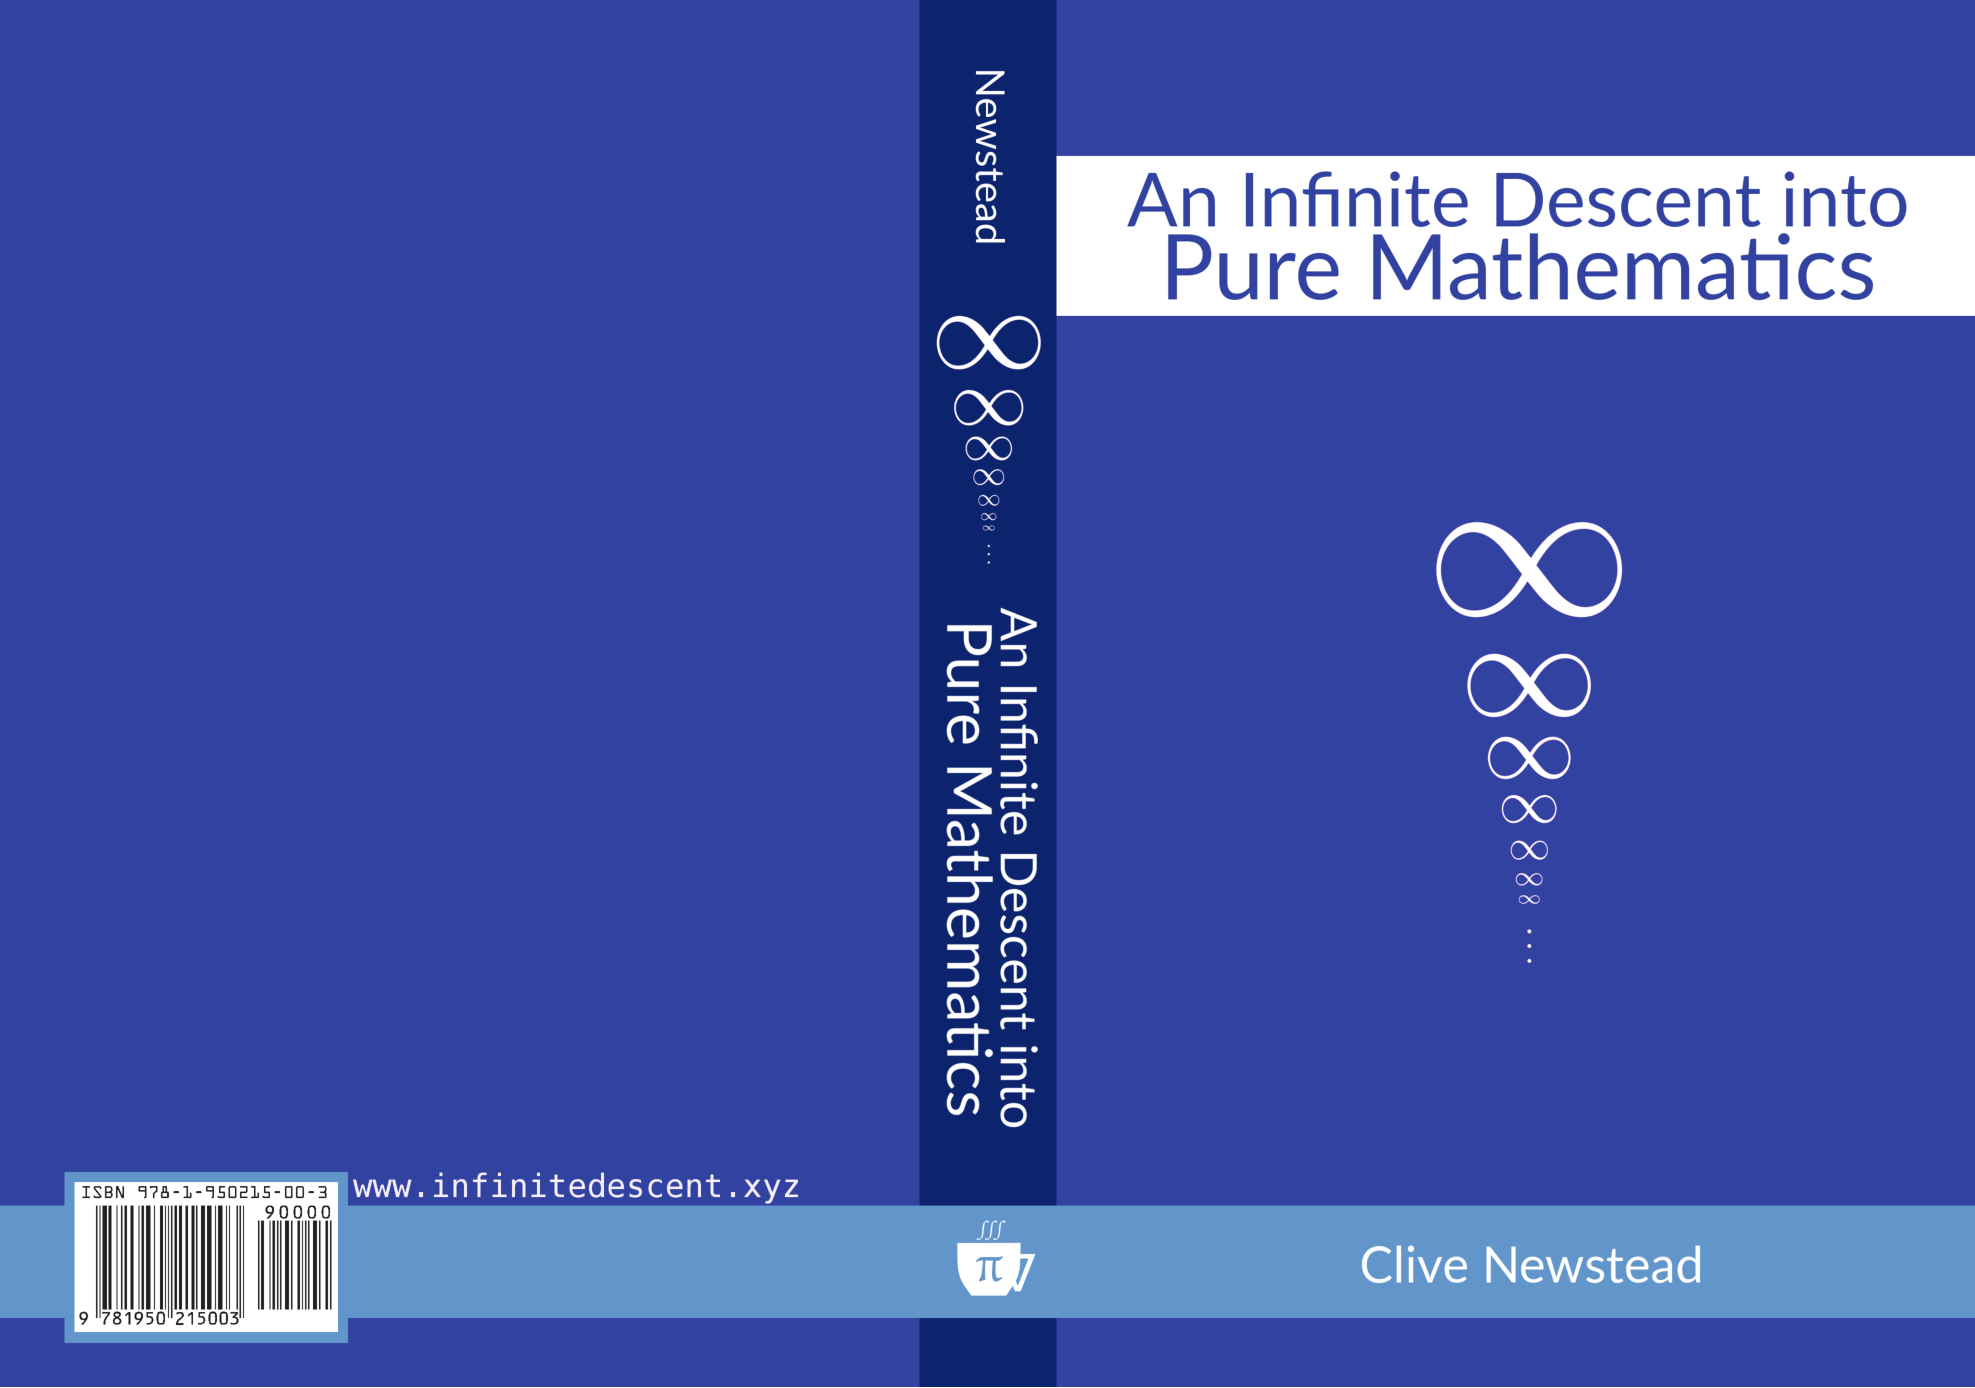
\includepdf[pages=-,fitpaper=true,noautoscale=false]{book/media/spread.pdf}

\frontmatter

% Title page
\newgeometry{centering,bindingoffset={0in}}
% !TeX root = ../../infdesc.tex

$ $

\vfill

\begin{center}
\thispagestyle{empty}

{\Huge \mdseries \fontfamily{bch}\selectfont
An Infinite Descent into\\
Pure Mathematics}

{\Large \mdseries \fontfamily{bch}\selectfont
Exercise Answers
}

\vfill
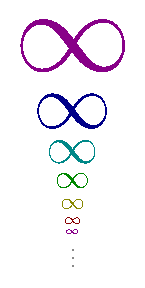
\includegraphics{book/media/logo.pdf}

\vfill


\textsc{by Fisher Yv}\\
\ifadapted{\textit{with adaptations by \adaptername}}

\vfill


\end{center}
\restoregeometry

\clearpage
% !TeX root = ../../infdesc.tex
{\small
~

\vfill

\thispagestyle{empty}
{%
This book is a collection of exercises and solutions to the book \textit{An Infinite Descent into Pure Mathematics}\\
\textcopyright{} 2023 Fisher Yv, All Rights Reserved.\\
\\
Original work of \textit{An Infinite Descent into Pure Mathematics}\\
\textcopyright{} 2023 Clive Newstead, All Rights Reserved.%
}{%

}


\begin{minipage}{0.75\textwidth}
\small
This book, its figures and its \TeX{} source are released under a Creative Commons Attribution--ShareAlike 4.0 International Licence. The full text of the licence is replicated at the end of the book, and can be found on the Creative Commons website:\\
\url{https://creativecommons.org/licenses/by/4.0/legalcode}
\end{minipage}

}

% Table of contents
\bookmark[page=3,level=0]{Contents}
\tableofcontents

\mainmatter

\setcounter{chapter}{-1}

% !TeX root = ../../infdesc.tex
\chapter{Getting started}
\markboth{Chapter \thechapter.\ Getting started}{Chapter \thechapter.\ Getting started}
\label{chGettingStarted}

\numberitemswithin{chapter}

% !TeX root = ../../infdesc.tex
\hintsection{\Cref*{chGettingStarted}}

Before we can start proving things, we need to eliminate certain kinds of statements that we might try to prove. Consider the following statement:

\begin{center}
\textit{This sentence is false.}
\end{center}

Is it true or false? If you think about this for a couple of seconds then you'll get into a bit of a pickle.

Now consider the following statement:

\begin{center}
\textit{The happiest donkey in the world.}
\end{center}

Is it true or false? Well it's not even a sentence; it doesn't make sense to even \textit{ask} if it's true or false!

Clearly we'll be wasting our time trying to write proofs of statements like the two listed above---we need to narrow our scope to statements that we might actually have a chance of proving (or perhaps refuting)! This motivates the following (informal) definition.

\begin{definition}
\label{defProposition}
\label{defProof}
\index{proposition}
\index{proof}
A \textbf{proposition} \index{proposition} is a statement to which it is possible to assign a \textbf{truth value} (`true' or `false'). If a proposition is true, a \textbf{proof} of the proposition is a logically valid argument demonstrating that it is true, which is pitched at such a level that a member of the intended audience can verify its correctness.
\end{definition}

Thus the statements given above are not propositions because there is no possible way of assigning them a truth value. Note that, in \Cref{defProposition}, all that matters is that it \textit{makes sense} to say that it is true or false, regardless of whether it actually \textit{is} true or false---the truth value of many propositions is unknown, even very simple ones.

\begin{exercise}
Think of an example of a true proposition, a false proposition, a proposition whose truth value you don't know, and a statement that is not a proposition.
\end{exercise}

Results in mathematical papers and textbooks may be referred to as \textit{propositions}, but they may also be referred to as \textit{theorems}, \textit{lemmas} or \textit{corollaries} depending on their intended usage.
\begin{itemize} 
\item A \textbf{proposition} is an umbrella term which can be used for any result.
\item A \textbf{theorem} is a key result which is particularly important.
\item A \textbf{lemma} is a result which is proved for the purposes of being used in the proof of a theorem. 
\item A \textbf{corollary} is a result which follows from a theorem without much additional effort.
\end{itemize}
These are not precise definitions, and they are not meant to be---you could call every result a \textit{proposition} if you wanted to---but using these words appropriately helps readers work out how to read a paper. For example, if you just want to skim a paper and find its key results, you'd look for results labelled as \textit{theorems}.

It is not much good trying to prove results if we don't have anything to prove results about. With this in mind, we will now introduce the \textit{number sets} and prove some results about them in the context of four topics, namely: division of integers, number bases, rational and irrational numbers, and polynomials. These topics will provide context for the material in \Cref{ptCoreConcepts}, and serve as an introduction to the topics covered in \Cref{ptTopics}.

We will not go into very much depth in this chapter. Rather, think of this as a warm-up exercise---a quick, light introduction, with more proofs to be provided in the rest of the book.

\subsection*{Sets}

Fundamental to mathematics is the notion of a \textit{set}. We will study sets in great detail in \Cref{chSets}, but you will find them in every chapter of the textbook, so we will take some time to think about them now. We will not treat sets formally at this stage---for now, the following definition will suffice.

\begin{definition}[to be revised in \Cref{defSet}]
\label{defSetsPreliminary}
\lindexmmc{in}{$\in$}
A \textbf{set} is a collection of objects. The objects in the set are called \textbf{elements} of the set. If $X$ is a set and $x$ is an object, then we write $x \in X$ \inlatexnb{x \textbackslash{}in X} to denote the assertion that $x$ is an element of $X$.
\end{definition}

The sets of concern to us first and foremost are the \textit{number sets}---that is, sets whose elements are particular types of \textit{number}. At this introductory level, many details will be temporarily swept under the rug; we will work at a level of precision which is appropriate for our current stage, but still allows us to develop a reasonable amount of intuition.

In order to define the number sets, we will need three things: an infinite line, a fixed point on this line, and a fixed unit of length.

So here we go. Here is an infinite line:
\begin{center}
\begin{tikzpicture}
\draw[latex-latex] (-5.5, 0) -- (5.5, 0) ;
\end{tikzpicture}
\end{center}
The arrows indicate that it is supposed to extend in both directions without end. The points on the line will represent numbers (specifically, \textit{real numbers}, a misleading term that will be defined in \Cref{defRealsInformal}).

Now let's fix a point on this line, and label it `$0$':
\begin{center}
\begin{tikzpicture}
\draw[latex-latex] (-5.5, 0) -- (5.5, 0) ; 
\draw (0, 0) -- (0, 0.1) node[above] {$0$} ;
\end{tikzpicture}
\end{center}
This point can be thought of as representing the number zero; it is the point against which all other numbers will be measured. Numbers to the left of $0$ on the number line are said to be \textit{negative}, and those to the right are \textit{positive}; $0$ itself is neither positive nor negative.

Finally, let's fix a unit of length:
\begin{center}
\begin{tikzpicture}
\draw (0, 0) -- (1, 0) ; 
\foreach \x in {0,1} \draw (\x, -0.1) -- (\x, 0.1)  ;
\end{tikzpicture}
\end{center}
This unit of length will be used, amongst other things, to compare the extent to which the other numbers differ from zero.

\begin{definition}
\label{defNumberLine}
The above infinite line, together with its fixed zero point and fixed unit length, constitute the (\textbf{real}) \textbf{number line}.
\end{definition}

We will use the number line to construct five sets of numbers of interest to us: the set $\mathbb{N}$ of \textit{natural numbers} (\Cref{defNaturalNumbersInformal}), the set $\mathbb{Z}$ of \textit{integers} (\Cref{defIntegersInformal}), the set $\mathbb{Q}$ of \textit{rational numbers} (\Cref{defRationalsInformal}), the $\mathbb{R}$ of \textit{real numbers} (\Cref{defRealsInformal}), and
the set $\mathbb{C}$ of \textit{complex numbers} (\Cref{defComplexNumbersInformal}).

Each of these sets has a different character and is used for different purposes, as we will seeu later in this chapter and throughout this book.

\subsection*{Natural numbers ($\mathbb{N}$)}

The \textit{natural numbers} are the numbers used for counting---they are the answers to questions of the form `how many'---for example, I have \textit{three} uncles, \textit{three} guinea pigs and \textit{zero} cats.

Counting is a skill humans have had for a very long time; we know this because there is evidence of people using tally marks tens of thousands of years ago. Tally marks provide one method of counting small numbers: starting with nothing, proceed through the objects you want to count one by one, and make a mark for every object. When you are finished, there will be as many marks as there are objects. We are taught from a young age to count with our fingers; this is another instance of making tally marks, where now instead of making a mark we raise a finger.

Making a tally mark represents an \textit{increment} in quantity---that is, adding one. On our number line, we can represent an increment in quantity by moving to the right by the unit length. Then the distance from zero we have moved, which is equal to the number of times we moved right by the unit length, is therefore equal to the number of objects being counted.

\begin{definition}
\label{defNaturalNumbersInformal}
The \textbf{natural numbers} are represented by the points on the number line which can be obtained by starting at $0$ and moving right by the unit length any number of times:
\begin{center}
\begin{tikzpicture}
\draw[latex-latex] (-5.5, 0) -- (5.5, 0) ; 
\foreach \x in {0,1,2,3,4,5} \draw (\x, 0) -- (\x, 0.1) node[above] {$\x$} ;
\end{tikzpicture}
\end{center}
In more familiar terms, they are the \textit{non-negative whole numbers}. We write $\mathbb{N}$ \inlatex{mathbb\{N\}}\lindexmmc{mathbb}{$\mathbb{A}, \mathbb{B}, \dots$} for the set of all natural numbers; thus, the notation `$n \in \mathbb{N}$' means that $n$ is a natural number.
\end{definition}

The natural numbers have very important and interesting mathematical structure, and are central to the material in \Cref{chCombinatorics}. A more precise characterisation of the natural numbers will be provided in \Cref{secPeanosAxioms}, and a mathematical construction of the set of natural numbers can be found in \Cref{secZFC} (see \Cref{cnsNaturalNumbersVonNeumann}). Central to these more precise characterisations will be the notions of `zero' and of `adding one'---just like making tally marks.

\begin{aside}
Some authors define the natural numbers to be the \textit{positive} whole numbers, thus excluding zero. We take $0$ to be a natural number since our main use of the natural numbers will be for counting finite sets, and a set with nothing in it is certainly finite! That said, as with any mathematical definition, the choice about whether $0 \in \mathbb{N}$ or $0 \not \in \mathbb{N}$ is a matter of taste or convenience, and is merely a convention---it is not something that can be proved or refuted.
\end{aside}

\subsection*{Number bases}

Writing numbers down is something that may seem easy to you now, but it likely took you several years as a child to truly understand what was going on. Historically, there have been many different systems for representing numbers symbolically, called \textit{numeral systems}.\index{numeral system} First came the most primitive of all, tally marks, appearing in the Stone Age and still being used for some purposes today. Thousands of years and hundreds of numeral systems later, there is one dominant numeral system, understood throughout the world: the \textbf{Hindu--Arabic numeral system}.\index{numeral system!Hindu--Arabic} This numeral system consists of ten symbols, called \textit{digits}. It is a \textit{positional} numeral system, meaning that the position of a symbol in a string determines its numerical value.

In English, the \textit{Arabic numerals} are used as the ten digits:
\[ 0 \quad 1 \quad 2 \quad 3 \quad 4 \quad 5 \quad 6 \quad 7 \quad 8 \quad 9 \]
The right-most digit in a string is in the units place, and the value of each digit increases by a factor of ten moving to the left. For example, when we write `$2812$', the left-most `$2$' represents the number two thousand, whereas the last `$2$' represents the number two.

The fact that there are ten digits, and that the numeral system is based on powers of ten, is a biological accident corresponding with the fact that most humans have ten fingers. For many purposes, this is inconvenient. For example, ten does not have many positive divisors (only four: $1$, $2$, $5$ and $10$)---this has implications for the ease of performing arithmetic; a system based on the number twelve, which has six positive divisors ($1$, $2$, $3$, $4$, $6$ and $12$), might be more convenient. Another example is in computing and digital electronics, where it is more convenient to work in a \textit{binary} system, with just two digits---$0$ and $1$---which represent `off' and `on' (or `low voltage' and `high voltage'), respectively; arithmetic can then be performed directly using sequences of \textit{logic gates} in an electrical circuit.

It is therefore worthwhile to have some understanding of positional numeral systems based on numbers other than ten. The mathematical abstraction we make leads to the definition of \textit{base-$b$ expansion}.

\begin{definition}
\label{defBaseBExpansionPreliminary}
\index{base-$b$ expansion}
\index{number base}
Let $b$ be a natural number greater than $1$. The \textbf{base-$b$ expansion} of a natural number $n$ is the\footnote{The use of the word `the' is troublesome here, since it assumes that every natural number has only one base-$b$ expansion. This fact actually requires proof---see \Cref{thmBaseBExpansion}.} string $d_r d_{r-1} \dots d_0$ such that:
\begin{enumerate}[(i)]
\item $n = d_r \cdot b^r + d_{r-1} \cdot b^{r-1} + \cdots + d_0 \cdot b^0$;
\item $0 \le d_i < b$ for each $i$; and
\item If $n>0$ then $d_r \ne 0$---the base-$b$ expansion of zero is $0$ in all bases $b$.
\end{enumerate}
Certain number bases have names; for instance, the base-$2$, $3$, $8$, $10$ and $16$ expansions are respectively called \textit{binary}, \textit{ternary}, \textit{octal}, \textit{decimal} and \textit{hexadecimal}.
\end{definition}

Before we look at an example of \Cref{defBaseBExpansionPreliminary} in action, let's examine the definition, which is a little terse on first sight.
\begin{itemize}
\item Condition (i) tells us that the digits in the string tell us how many of each power of $b$ are added up to obtain $n$. For example, when $b=10$, the digits from right to left tell us the units, tens, hundreds, thousands, and so on.
\item Condition (ii) tells us that the digits in a base-$b$ expansion must be less than $b$---for example, the base-$4$ digits are $0$, $1$, $2$ and $3$. If we allowed more digits then silly things would happen---for example, if `$\mathrm{X}$' were a new base-$10$ digit representing the number ten, then `$\mathrm{X}2$' and `$102$' would be different strings both representing the number one hundred and two.
\item Condition (iii) ensures that the string representing a positive number doesn't have any leading `$0$'s---otherwise, for example, `$01423$' and `$1423$' would be different strings representing the same natural number.
\end{itemize}

\begin{example}
Consider the number $1023$. Its decimal (base-$10$) expansion is $1023$, since
\[ 1023 = 1 \cdot 10^3 + 0 \cdot 10^2 + 2 \cdot 10^1 + 3 \cdot 10^0 \]
Its binary (base-$2$) expansion is $1111111111$, since
\[ 1023 = 1 \cdot 2^9 + 1 \cdot 2^8 + 1 \cdot 2^7 + 1 \cdot 2^6 + 1 \cdot 2^5 + 1 \cdot 2^4 + 1 \cdot 2^3 + 1 \cdot 2^2 + 1 \cdot 2^1 + 1 \cdot 2^0 \]
We can express numbers in base-$36$ by using the ten usual digits $0$ through $9$ and the twenty-six letters $\mathrm{A}$ through $\mathrm{Z}$; for instance, $\mathrm{A}$ represents $10$, $\mathrm{M}$ represents $22$ and $\mathrm{Z}$ represents $35$. The base-$36$ expansion of $1023$ is $\mathrm{SF}$, since
\[ 1023 = 28 \cdot 36^1 + 15 \cdot 36^0 = \mathrm{S} \cdot 36^1 + \mathrm{F} \cdot 36^0 \]
\end{example}

\begin{exercise}
Find the binary, ternary, octal, decimal, hexadecimal and base-$36$ expansions of the number $21127$, using the letters $\mathrm{A}$--$\mathrm{F}$ as additional digits for the hexadecimal expansion (representing the numbers $10$--$15$, respectively), and the letters $\mathrm{A}$--$\mathrm{Z}$ as additional digits for the base-$36$ expansion.
\end{exercise}

We sometimes wish to specify a natural number in terms of its base-$b$ expansion; we have some notation for this.

\begin{notation}
Let $b>1$. If the numbers $d_0,d_1,\dots,d_r$ are base-$b$ digits (in the sense of \Cref{defBaseBExpansionPreliminary}), then we write
\[ {d_rd_{r-1} \dots d_0}_{(b)} = d_r \cdot b^r + d_{r-1} \cdot b^{r-1} + \cdots + d_0 \cdot b^0 \]
for the natural number whose base-$b$ expansion is $d_rd_{r-1} \dots d_0$. If there is no subscript $(b)$ and a base is not specified explicitly, the expansion will be assumed to be in base-$10$.
\end{notation}

\begin{example}
Using our new notation, we have
\[ 1023 = 1111111111_{(2)} = 1101220_{(3)} = 1777_{(8)} = 1023_{(10)} = 3\mathrm{FF}_{(16)} = \mathrm{SF}_{(36)} \]
\end{example}

\subsection*{Integers ($\mathbb{Z}$)}

The \textit{integers} can be used for measuring the difference between two natural numbers. For example, suppose I have five apples and five bananas. Another person, also holding apples and bananas, wishes to trade. After our exchange, I have seven apples and only one banana. Thus I have two more apples and four fewer bananas.

Since an increment in quantity can be represented by moving to the right on the number line by the unit length, a \textit{decrement} in quantity can therefore be represented by moving to the \textit{left} by the unit length. Doing so gives rise to the integers.

\begin{definition}
\label{defIntegersInformal}
The \textbf{integers} are represented by the points on the number line which can be obtained by starting at $0$ and moving in either direction by the unit length any number of times:
\begin{center}
\begin{tikzpicture}
\draw[latex-latex] (-5.5, 0) -- (5.5, 0) ; 
\foreach \x in {-5,-4,-3,-2,-1,0,1,2,3,4,5} \draw (\x, 0) -- (\x, 0.1) node[above] {$\x$} ;
\end{tikzpicture}
\end{center}
We write $\mathbb{Z}$ \inlatex{mathbb\{Z\}}\lindexmmc{mathbb}{$\mathbb{A}, \mathbb{B}, \dots$} for the set of all integers; thus, the notation `$n \in \mathbb{Z}$' means that $n$ is an integer.
\end{definition}

The integers have such a fascinating structure that a whole chapter of this book is devoted to them---see \Cref{chNumberTheory}. This is to do with the fact that, although you can add, subtract and multiply two integers and obtain another integer, the same is not true of division. This `bad behaviour' of division is what makes the integers interesting. We will now see some basic results about division.

\subsection*{Division of integers}
\label{pGettingStartedDivision}

The motivation we will soon give for the definition of the rational numbers (\Cref{defRationalsInformal}) is that the result of dividing one integer by another integer is not necessarily another integer. However, the result is \textit{sometimes} another integer; for example, I can divide six apples between three people, and each person will receive an integral number of apples. This makes division interesting: how can we measure the failure of one integer's divisibility by another? How can we deduce when one integer is divisible by another? What is the structure of the set of integers when viewed through the lens of division? This motivates \Cref{defDivisionPreliminary}.

\begin{definition}[to be repeated in \Cref{defDivision}]
\label{defDivisionPreliminary}
\index{division}
\index{divisor}
\index{factor}
\index{multiple}
Let $a,b \in \mathbb{Z}$. We say $b$ \textbf{divides} $a$ if $a=qb$ for some integer $q$. There are many other ways of saying that $b$ divides $a$, such as: $a$ is \textit{divisible by} $b$, $b$ is a \textit{divisor} of $a$, $b$ is a \textit{factor} of $a$, or $a$ is a \textit{multiple} of $b$.
\end{definition}

Note that, perhaps counterintuitively, the definition if divisibility does not involve the arithmetic operation of division: it is defined in terms of multiplication.

\begin{example}
The integer $12$ is divisible by $1$, $2$, $3$, $4$, $6$ and $12$, since
\[ 12 = 12 \cdot 1 = 6 \cdot 2 = 4 \cdot 3 = 3 \cdot 4 = 2 \cdot 6 = 1 \cdot 12 \]
It is also divisible by the negatives of all of those numbers; for example, $12$ is divisible by $-3$ since $12 = (-4) \cdot (-3)$.
\end{example}

\begin{exercise}
\label{exOneDividesEveryIntegerDividesZero}
Prove that $1$ divides every integer, and that every integer divides $0$.
\end{exercise}

A consequence of \Cref{exOneDividesEveryIntegerDividesZero} is that $0$ is divisible by $0$. This is surprising: we've been told our whole lives that we can't divide by zero, but now we discover that we can divide zero by zero\dots{} how can that be? This highlights why it was so important for the definition of divisibility (\Cref{defDivisionPreliminary}) to be given in terms of multiplication, without using the division operation: saying that $0$ divides $0$ simply means that $0$ can be multiplied by an integer to obtain $0$ (which is true)---but this does not imply that the expression `$\frac{0}{0}$' can (or should) be meaningfully defined.

Using \Cref{defDivisionPreliminary}, we can prove some general basic facts about divisibility.

\begin{proposition}
\label{propDivisibilityIsTransitive}
Let $a,b,c \in \mathbb{Z}$. If $c$ divides $b$ and $b$ divides $a$, then $c$ divides $a$.
\end{proposition}

\begin{cproof}
Suppose that $c$ divides $b$ and $b$ divides $a$. By \Cref{defDivisionPreliminary}, it follows that
\[ b=qc \quad \text{and} \quad a=rb \]
for some integers $q$ and $r$. Using the first equation, we may substitute $qc$ for $b$ in the second equation, to obtain
\[ a=r(qc) \]
But $r(qc) = (rq)c$, and $rq$ is an integer, so it follows from \Cref{defDivisionPreliminary} that $c$ divides $a$.
\end{cproof}

% To do: draw attention to the wording of the proof, and the 'unpack definition - do something - apply definition' style of the proof.

\begin{exercise}
\label{exDivisibilityIsLinear}
Let $a,b,d \in \mathbb{Z}$. Suppose that $d$ divides $a$ and $d$ divides $b$. Given integers $u$ and $v$, prove that $d$ divides $au+bv$.
\end{exercise}

Some familiar concepts, such as evenness and oddness, can be characterised in terms of divisibility.

\begin{definition}
\label{defEvenOdd}
\index{even!integer}
\index{odd!integer}
An integer $n$ is \textbf{even} if it is divisible by $2$; otherwise, $n$ is \textbf{odd}.
\end{definition}

It is not just interesting to know when one integer \textit{does} divide another; however, proving that one integer \textit{doesn't} divide another is much harder. Indeed, to prove that an integer $b$ does not divide an integer $a$, we must prove that $a \ne qb$ for \textit{any} integer $q$ at all. We will look at methods for doing this in \Cref{chLogicalStructure}; these methods use the following extremely important result, which will underlie all of \Cref{chNumberTheory}.

\begin{theorem}[Division theorem, to be repeated in \Cref{thmDivisionTheorem}]
\label{thmDivisionPreliminary}
\index{division theorem}
Let $a,b \in \mathbb{Z}$ with $b \ne 0$. There is exactly one way to write
\[ a = qb + r \]
such that $q$ and $r$ are integers, and $0 \le r < b$ (if $b > 0$) or $0 \le r < -b$ (if $b < 0$).
\end{theorem}

The number $q$ in \Cref{thmDivisionPreliminary} is called the \textbf{quotient}\index{quotient} of $a$ when divided by $b$, and the number $r$ is called the \textbf{remainder}\index{remainder}.

\begin{example}
The number $12$ leaves a remainder of $2$ when divided by $5$, since $12 = 2 \cdot 5 + 2$.
\end{example}

Here's a slightly more involved example.

\begin{proposition}
Suppose an integer $a$ leaves a remainder of $r$ when divided by an integer $b$, and that $r>0$. Then $-a$ leaves a remainder of $b-r$ when divided by $b$.
\end{proposition}

\begin{cproof}
Suppose $a$ leaves a remainder of $r$ when divided by $b$. Then
\[ a=qb+r \]
for some integer $q$. A bit of algebra yields
\[ -a = -qb-r = -qb-r+(b-b) = -(q+1)b + (b-r) \]
Since $0<r<b$, we have $0<b-r<b$. Hence $-(q+1)$ is the quotient of $-a$ when divided by $b$, and $b-r$ is the remainder.
\end{cproof}

\begin{exercise}
Prove that if an integer $a$ leaves a remainder of $r$ when divided by an integer $b$, then $a$ leaves a remainder of $r$ when divided by $-b$.
\end{exercise}

We will finish this part on division of integers by connecting it with the material on number bases---we can use the division theorem (\Cref{thmDivisionPreliminary}) to find the base-$b$ expansion of a given natural number. It is based on the following observation: the natural number $n$ whose base-$b$ expansion is $d_rd_{r-1} \cdots d_1 d_0$ is equal to
\[ d_0 + b(d_1 + b(d_2 + \cdots + b(d_{r-1} + bd_r) \cdots)) \]
Moreover, $0 \le d_i < b$ for all $i$. In particular $n$ leaves a remainder of $d_0$ when divided by $b$. Hence
\[ \frac{n-d_0}{b} = d_1 + d_2b + \cdots + d_rb^{r-1} \]
The base-$b$ expansion of $\frac{n-d_0}{b}$ is therefore
\[ d_rd_{r-1} \cdots d_1 \]
In other words, the remainder of $n$ when divided by $b$ is the last base-$b$ digit of $n$, and then subtracting this number from $n$ and dividing the result by $b$ truncates the final digit. Repeating this process gives us $d_1$, and then $d_2$, and so on, until we end up with $0$.

This suggests the following algorithm for computing the base-$b$ expansion of a number $n$:
\begin{itemize}
\item \textbf{Step 1.} Let $d_0$ be the remainder when $n$ is divided by $b$, and let $n_0=\frac{n-d_0}{b}$ be the quotient. Fix $i=0$.
\item \textbf{Step 2.} Suppose $n_i$ and $d_i$ have been defined. If $n_i=0$, then proceed to Step 3. Otherwise, define $d_{i+1}$ to be the remainder when $n_i$ is divided by $b$, and define $n_{i+1} = \frac{n_i-d_{i+1}}{b}$. Increment $i$, and repeat Step 2.
\item \textbf{Step 3.} The base-$b$ expansion of $n$ is
\[ d_id_{i-1} \cdots d_0 \]
\end{itemize}

\begin{example}
We compute the base-$17$ expansion of $15213$, using the letters $\mathrm{A}$--$\mathrm{G}$ to represent the numbers $10$ through $16$.
\begin{itemize}
\item $15213 = 894 \cdot 17 + 15$, so $d_0=15=\mathrm{F}$ and $n_0=894$.
\item $894 = 52 \cdot 17 + 10$, so $d_1=10 = \mathrm{A}$ and $n_1=52$.
\item $52 = 3 \cdot 17 + 1$, so $d_2 = 1$ and $n_2=3$.
\item $3 = 0 \cdot 17 + 3$, so $d_3 = 3$ and $n_3=0$.
\item The base-$17$ expansion of $15213$ is therefore $31\mathrm{AF}$.
\end{itemize}
A quick verification gives
\[ 31\mathrm{AF}_{(17)} = 3 \cdot 17^3 + 1 \cdot 17^2 + 10 \cdot 17 + 15 = 15213 \]
as desired.
\end{example}

\begin{exercise}
Find the base-$17$ expansion of $408\,735\,787$ and the base-$36$ expansion of $1\,442\,151\,747$.
\end{exercise}

\subsection*{Rational numbers ($\mathbb{Q}$)}

Bored of eating apples and bananas, I buy a pizza which is divided into eight slices. A friend and I decide to share the pizza. I don't have much of an appetite, so I eat three slices and my friend eats five. Unfortunately, we cannot represent the proportion of the pizza each of us has eaten using natural numbers or integers. However, we're not far off: we can count the number of equal parts the pizza was split into, and of those parts, we can count how many we had. On the number line, this could be represented by splitting the unit line segment from $0$ to $1$ into eight equal pieces, and proceeding from there. This kind of procedure gives rise to the \textit{rational numbers}.

\begin{definition}
\label{defRationalsInformal}
The \textbf{rational numbers} are represented by the points at the number line which can be obtained by dividing any of the unit line segments between integers into an equal number of parts.
\begin{center}
\begin{tikzpicture}
\draw[latex-latex] (-5.5, 0) -- (5.5, 0) ; 
\foreach \x in {-5,-4,-3,-2,-1,0,1,2,3,4,5} \draw (\x, 0) -- (\x, 0.25) node[above] {$\x$} ;
\foreach \x in {-5,-4,-3,-2,-1,0,1,2,3,4,5} {
  \foreach \i in {-0.33,0.33} {
    \draw (\x+\i, 0) -- (\x+\i, 0.15) ;
  }
}
\end{tikzpicture}
\end{center}
The rational numbers are those of the form $\frac{a}{b}$, where $a,b \in \mathbb{Z}$ and $b \ne 0$. We write $\mathbb{Q}$ \inlatex{mathbb\{Q\}}\lindexmmc{mathbb}{$\mathbb{A}, \mathbb{B}, \dots$} for the set of all rational numbers; thus, the notation `$q \in \mathbb{Q}$' means that $q$ is a rational number.
\end{definition}

The rational numbers are a very important example of a type of algebraic structure known as a \textit{field}---they are particularly central to algebraic number theory and algebraic geometry.

\subsection*{Real numbers ($\mathbb{R}$)}

Quantity and change can be measured in the abstract using \textit{real numbers}.

\begin{definition}
\label{defRealsInformal}
The \textbf{real numbers} are the points on the number line. We write $\mathbb{R}$ \inlatex{mathbb\{R\}}\lindexmmc{mathbb}{$\mathbb{A}, \mathbb{B}, \dots$} for the set of all real numbers; thus, the notation `$a \in \mathbb{R}$' means that $a$ is a real number.
\end{definition}

The real numbers are central to real analysis, a branch of mathematics introduced in \Cref{chRealNumbers}. They turn the rationals into a \textit{continuum} by `filling in the gaps'---specifically, they have the property of \textit{completeness}, meaning that if a quantity can be approximated with arbitrary precision by real numbers, then that quantity is itself a real number.

We can define the basic arithmetic operations (addition, subtraction, multiplication and division) on the real numbers, and a notion of ordering of the real numbers, in terms of the infinite number line.

\begin{itemize}
\item \textbf{Ordering.} A real number $a$ is less than a real number $b$, written $a<b$, if $a$ lies to the left of $b$ on the number line. The usual conventions for the symbols $\le$ \inlatex{le}\lindexmmc{le}{$\le$}, $>$ and $\ge$ \inlatex{ge}\lindexmmc{ge}{$\ge$} apply, for instance `$a \le b$' means that either $a < b$ or $a = b$.

\item \textbf{Addition.} Suppose we want to add a real number $a$ to a real number $b$. To do this, we \textit{translate} $a$ by $b$ units to the right---if $b<0$ then this amounts to translating $a$ by an equivalent number of units to the left. Concretely, take two copies of the number line, one above the other, with the same choice of unit length; move the $0$ of the lower number line beneath the point $a$ of the upper number line. Then $a+b$ is the point on the upper number line lying above the point $b$ of the lower number line.

Here is an illustration of the fact that $(-3) + 5 = 2$:

\begin{center}
\fitwidthc{0.9}{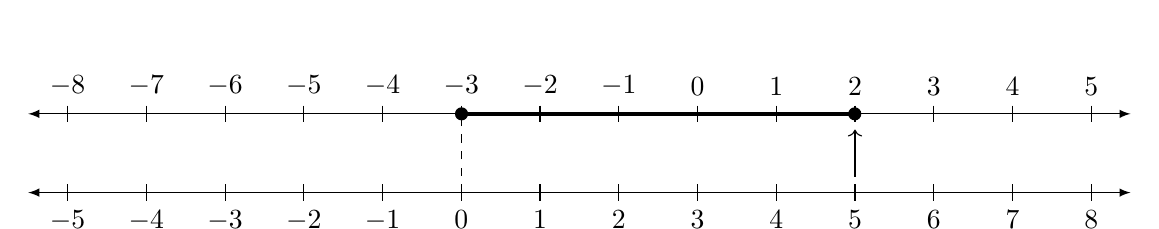
\begin{tikzpicture}
% Adapted from http://tex.stackexchange.com/questions/148252/
\draw[latex-latex] (-8.5,0) -- (5.5,0) ; 
\foreach \x in  {-8,-7,-6,-5,-4,-3,-2,-1,0,1,2,3,4,5}
\draw[shift={(\x,0)}] (0pt,3pt) -- (0pt,-3pt);
\foreach \x in {-8,-7,-6,-5,-4,-3,-2,-1,0,1,2,3,4,5}
\draw[shift={(\x,0)}] (0pt,0pt) -- (0pt,3pt) node[above] {$\x$};
\draw[*-*] (-3.08,0) -- (2.08,0);
\draw[very thick] (-3,0) -- (2,0);

\draw[latex-latex] (-8.5,-1) -- (5.5,-1) ; 
\foreach \x in  {-5,-4,-3,-2,-1,0,1,2,3,4,5,6,7,8}
\draw[shift={(\x-3,-1)},color=black] (0pt,3pt) -- (0pt,-3pt);
\foreach \x in {-5,-4,-3,-2,-1,0,1,2,3,4,5,6,7,8}
\draw[shift={(\x-3,-1)},color=black] (0pt,0pt) -- (0pt,-3pt) node[below] {$\x$};
\draw[dashed] (-3,-1) -- (-3,0) ;
\draw[->] (2,-0.8) -- (2,-0.2) ;
\end{tikzpicture}}
\end{center}

\item \textbf{Multiplication.} This one is fun. Suppose we want to multiply a real number $a$ by a real number $b$. To do this, we \textit{scale} the number line, and perhaps \textit{reflect} it. Concretely, take two copies of the number line, one above the other; align the $0$ points on both number lines, and stretch the lower number line evenly until the point $1$ on the lower number line is below the point $a$ on the upper number line---note that if $a<0$ then the number line must be reflected in order for this to happen. Then $a \cdot b$ is the point on the upper number line lying above $b$ on the lower number line.

Here is an illustration of the fact that $5 \cdot 4 = 20$.

\begin{center}
\fitwidthc{0.9}{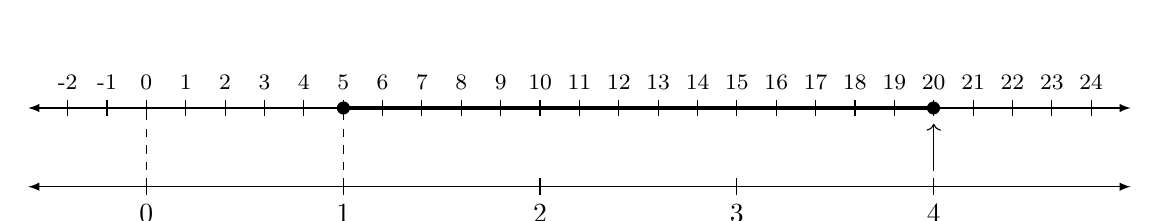
\begin{tikzpicture}
% Adapted from http://tex.stackexchange.com/questions/148252/
\draw[latex-latex] (-5.5,0) -- (8.5,0) ; 
\foreach \x in  {-2,-1,0,1,2,3,4,5,6,7,8,9,10,11,12,13,14,15,16,17,18,19,20,21,22,23,24}
\draw[shift={(0.5*\x-4,0)}] (0pt,3pt) -- (0pt,-3pt);
\foreach \x in {-2,-1,0,1,2,3,4,5,6,7,8,9,10,11,12,13,14,15,16,17,18,19,20,21,22,23,24}
\draw[shift={(0.5*\x-4,0)}] (0pt,0pt) -- (0pt,3pt) node[above] {$\text{\footnotesize\x}$};
\draw[*-*] (-1.58,0) -- (6.08,0);
\draw[very thick] (-1.5,0) -- (6,0);

\draw[latex-latex] (-5.5,-1) -- (8.5,-1) ; 
\foreach \x in  {0,1,2,3,4}
\draw[shift={(2.5*\x-4,-1)},color=black] (0pt,3pt) -- (0pt,-3pt);
\foreach \x in {0,1,2,3,4}
\draw[shift={(2.5*\x-4,-1)},color=black] (0pt,0pt) -- (0pt,-3pt) node[below] {$\x$};
\draw[dashed] (-4,-1) -- (-4,0) ;
\draw[dashed] (-1.5,-1) -- (-1.5,0) ;
\draw[->] (6,-0.8) -- (6,-0.2) ;
\end{tikzpicture}}
\end{center}

and here is an illustration of the fact that $(-5) \cdot 4 = -20$:
\begin{center}
\fitwidthc{0.9}{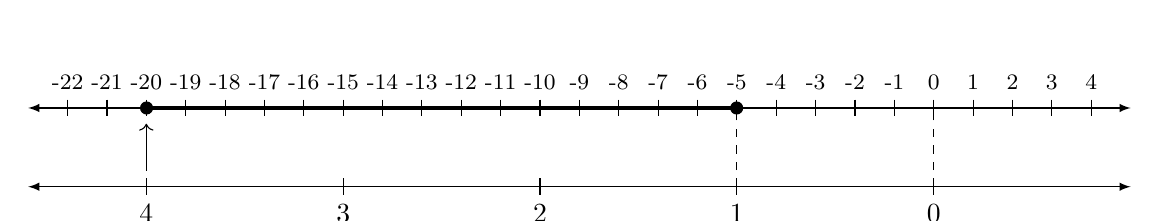
\begin{tikzpicture}
% Adapted from http://tex.stackexchange.com/questions/148252/
\draw[latex-latex] (-5.5,0) -- (8.5,0) ; 
\foreach \x in  {-22,-21,...,4}
\draw[shift={(0.5*\x+6,0)}] (0pt,3pt) -- (0pt,-3pt);
\foreach \x in {-22,-21,...,4}
\draw[shift={(0.5*\x+6,0)}] (0pt,0pt) -- (0pt,3pt) node[above] {$\text{\footnotesize\x}$};
\draw[*-*] (-4.08,0) -- (3.58,0);
\draw[very thick] (-4,0) -- (3.5,0);

\draw[latex-latex] (-5.5,-1) -- (8.5,-1) ; 
\foreach \x in  {0,1,2,3,4}
\draw[shift={(6-2.5*\x,-1)},color=black] (0pt,3pt) -- (0pt,-3pt);
\foreach \x in {0,1,2,3,4}
\draw[shift={(6-2.5*\x,-1)},color=black] (0pt,0pt) -- (0pt,-3pt) node[below] {$\x$};
\draw[dashed] (6,-1) -- (6,0) ;
\draw[dashed] (3.5,-1) -- (3.5,0) ;
\draw[->] (-4,-0.8) -- (-4,-0.2) ;
\end{tikzpicture}}
\end{center}
\end{itemize}

\begin{exercise}
Interpret the operations of subtraction and division as geometric transformations of the real number line.
\end{exercise}

We will take for granted the arithmetic properties of the real numbers in this chapter, waiting until \Cref{secInequalitiesMeans} to sink our teeth into the details. For example, we will take for granted the basic properties of rational numbers, for instance
\[ \frac{a}{b}+\frac{c}{d} = \frac{ad+bc}{bd} \quad \text{and} \quad \frac{a}{b} \cdot \frac{c}{d} = \frac{ac}{bd} \]

\subsection*{Rational and irrational numbers}
\label{pGettingStartedRationalNumbers}

Before we can talk about irrational numbers, we should say what they are.

\begin{definition}
\label{defIrrationalNumber}
\index{irrational number}
An \textbf{irrational number} is a real number that is not rational.
\end{definition}

Unlike $\mathbb{N},\mathbb{Z},\mathbb{Q},\mathbb{R},\mathbb{C}$, there is no standard single letter expressing the irrational numbers. However, by the end of \Cref{secSetOperations}, we will be able to write the set of irrational numbers as `$\mathbb{R} \setminus \mathbb{Q}$'.

Proving that a real number is \textit{irrational} is not particularly easy, in general. We will get our foot in the door by allowing ourselves to assume the following result, which is restated and proved in \Cref{propSqrt2Irrational}.

\begin{proposition}
\label{propSqrt2IrrationalPreliminary}
The real number $\sqrt{2}$ is irrational. \qed
\end{proposition}

% To do: include proof, note that we will prove that fractions can be cancelled to lowest terms later.

We can use the fact that $\sqrt{2}$ is irrational to prove some facts about the relationship between rational numbers and irrational numbers.

\begin{proposition}
Let $a$ and $b$ be irrational numbers. It is possible that $ab$ be rational.
\end{proposition}

\begin{cproof}
Let $a=b=\sqrt{2}$. Then $a$ and $b$ are irrational, and $ab=2=\frac{2}{1}$, which is rational.
\end{cproof}

\begin{exercise}
Let $r$ be a rational number and let $a$ be an irrational number. Prove that it is possible that $ra$ be rational, and it is possible that $ra$ be irrational.
\end{exercise}

% To do: set-builder notation and intervals

\subsection*{Complex numbers ($\mathbb{C}$)}

We have seen that multiplication by real numbers corresponds with scaling and reflection of the number line---scaling alone when the multiplicand is positive, and scaling with reflection when it is negative. We could alternatively interpret this reflection as a \textit{rotation} by half a turn, since the effect on the number line is the same. You might then wonder what happens if we rotate by arbitrary angles, rather than only half turns.

What we end up with is a \textit{plane} of numbers, not merely a line---see \Cref{figComplexNumbers}. Moreover, it happens that the rules that we expect arithmetic operations to satisfy still hold---addition corresponds with translation, and multiplication corresponds with scaling and rotation. This resulting number set is that of the \textit{complex numbers}.

\begin{definition}
\label{defComplexNumbersInformal}
The \textbf{complex numbers} are those obtained by the non-negative real numbers upon rotation by any angle about the point $0$. We write $\mathbb{C}$ \inlatex{mathbb\{C\}}\lindexmmc{mathbb}{$\mathbb{A}, \mathbb{B}, \dots$} for the set of all complex numbers; thus, the notation `$z \in \mathbb{C}$' means that $z$ is a complex number.
\end{definition}

\begin{figure}[p!]
\centering
\resizebox{\textwidth}{!}{
\begin{tikzpicture}
\draw[latex-latex] (-5.5,0) -- (5.5,0) ;
\draw[latex-latex, dotted] (-4.76, 2.75) -- (4.76, -2.75) ;
\draw[latex-latex, dotted] (-2.75, 4.76) -- (2.75, -4.76) ;
\draw[latex-latex, dotted] (0, -5.5) -- (0, 5.5) ;
\draw[latex-latex, dotted] (2.75, 4.76) -- (-2.75, -4.76) ;
\draw[latex-latex, dotted] (4.76, 2.75) -- (-4.76, -2.75) ;
\draw[dotted] (0,0) circle [radius=1] ;
\draw[dotted] (0,0) circle [radius=2] ;
\draw[dotted] (0,0) circle [radius=3] ;
\draw[dotted] (0,0) circle [radius=4] ;
\draw[dotted] (0,0) circle [radius=5] ;
\foreach \x in  {-5,-4,-3,-2,-1,0,1,2,3,4,5}
  \draw[shift={(\x,0)}] (0pt,3pt) -- (0pt,-3pt);
\foreach \x in {-5,-4,-3,-2,-1,0,1,2,3,4,5}
  \draw[shift={(\x,0)}] (0,0) node[below right] {$\text{\small\x}$};
\draw (0,1) node[above right] {$i$};
\draw (-3pt,1) -- (3pt,1);
\foreach \x in {2,3,4,5}
  \draw[shift={(0,\x)}] (0,0) node[above right] {$\x i$};
\foreach \x in {2,3,4,5}
  \draw[shift={(0,\x)}] (-3pt,0pt) -- (3pt, 0pt);
\foreach \x in {2,3,4,5}
  \draw[shift={(0,-\x)}] (0,0) node[below right] {$\text{\small-}\x i$};
\foreach \x in {2,3,4,5}
  \draw[shift={(0,-\x)}] (-3pt,0pt) -- (3pt, 0pt);
\draw (0,-1) node[below right] {$\text{\small-}i$};
\draw (-3pt,-1) -- (3pt,-1);
\end{tikzpicture}
}
\caption{Illustration of the complex plane, with some points labelled.}
\label{figComplexNumbers}
\end{figure}

There is a particularly important complex number, $i$, which is the point in the complex plane exactly one unit above $0$---this is illustrated in \Cref{figComplexNumbers}. Multiplication by $i$ has the effect of rotating the plane by a quarter turn anticlockwise. In particular, we have $i^2 = i \cdot i = -1$; the complex numbers have the astonishing property that square roots of \textit{all} complex numbers exist (including all the real numbers).

In fact, every complex number can be written in the form $a+bi$, where $a,b \in \mathbb{R}$; this number corresponds with the point on the complex plane obtained by moving $a$ units to the right and $b$ units up, reversing directions as usual if $a$ or $b$ is negative. Arithmetic on the complex numbers works just as with the real numbers; in particular, using the fact that $i^2=-1$, we obtain
\[ (a+bi)+(c+di) = (a+c)+(b+d)i \quad \text{and} \quad (a+bi) \cdot (c+di) = (ac-bd) + (ad+bc)i \]

We will discuss complex numbers further in the portion of this chapter on polynomials below.

\subsection*{Polynomials}
\label{pGettingStartedPolynomials}

The natural numbers, integers, rational numbers, real numbers and complex numbers are all examples of \textit{semirings}, which means that they come equipped with nicely behaving notions of addition and multiplication.

\begin{definition}
\label{defPolynomialPreliminary}
\index{polynomial}
Let $\mathbb{S} = \mathbb{N}$, $\mathbb{Z}$, $\mathbb{Q}$, $\mathbb{R}$ or $\mathbb{C}$. A (\textbf{univariate}) \textbf{polynomial over $\mathbb{S}$} in the \textbf{indeterminate} $x$ is an expression of the form
\[ a_0 + a_1x + \cdots + a_nx^n \]
where $n \in \mathbb{N}$ and each $a_k \in \mathbb{S}$. The numbers $a_k$ are called the \textbf{coefficients} of the polynomial. If not all coefficients are zero, the largest value of $k$ for which $a_k \ne 0$ is called the \textbf{degree} of the polynomial. By convention, the degree of the polynomial $0$ is $-\infty$.
\end{definition}

Polynomials of degree $1$, $2$, $3$, $4$ and $5$ are respectively called \textit{linear}, \textit{quadratic}, \textit{cubic}, \textit{quartic} and \textit{quintic} polynomials.

\begin{example}
The following expressions are all polynomials:
\[ 3 \qquad 2x-1 \qquad (3+i)x^2-x \]
Their degrees are $0$, $1$ and $2$, respectively. The first two are polynomials over $\mathbb{Z}$, and the third is a polynomial over $\mathbb{C}$.
\end{example}

\begin{exercise}
Write down a polynomial of degree $4$ over $\mathbb{R}$ which is not a polynomial over $\mathbb{Q}$.
\end{exercise}

\begin{notation}
Instead of writing out the coefficients of a polynomial each time, we may write something like $p(x)$ or $q(x)$. The `$(x)$' indicates that $x$ is the indeterminate of the polynomial. If $\alpha$ is a number\footnote{When dealing with polynomials, we will typically reserve the letter $x$ for the indeterminate variable, and use the Greek letters $\alpha,\beta,\gamma$ \inlatex{alpha, \textbackslash{}beta, \textbackslash{}gamma} for numbers to be substituted into a polynomial.} and $p(x)$ is a polynomial in indeterminate $x$, we write $p(\alpha)$ for the result of \textbf{substituting} $\alpha$ for $x$ in the expression $p(x)$.
\end{notation}

Note that, if $A$ is any of the sets $\mathbb{N}$, $\mathbb{Z}$, $\mathbb{Q}$, $\mathbb{R}$ or $\mathbb{C}$, and $p(x)$ is a polynomial over $A$, then $p(\alpha) \in A$ for all $\alpha \in A$.

\begin{example}
Let $p(x)=x^3-3x^2+3x-1$. Then $p(x)$ is a polynomial over $\mathbb{Z}$ with indeterminate $x$. For any integer $\alpha$, the value $p(\alpha)$ will also be an integer. For example
\[ p(0) = 0^3-3 \cdot 0^2 + 3 \cdot 0 - 1 = -1 \quad \text{and} \quad p(3) = 3^3 - 3 \cdot 3^2 + 3 \cdot 3 - 1 = 8 \]
\end{example}

\begin{definition}
\label{defRootOfPolynomial}
\index{root}
Let $p(x)$ be a polynomial. A \textbf{root} of $p(x)$ is a complex number $\alpha$ such that $p(\alpha)=0$.
\end{definition}

The \textit{quadratic formula} (\Cref{thmQuadraticFormula}) tells us that the roots of the polynomial $x^2+ax+b$, where $a,b \in \mathbb{C}$, are precisely the complex numbers
\[ \frac{-a+\sqrt{a^2-4b}}{2} \quad \text{and} \quad \frac{-a-\sqrt{a^2-4b}}{2} \]

Note our avoidance of the symbol `$\pm$', which is commonly found in discussions of quadratic polynomials. The symbol `$\pm$' is dangerous because it may suppress the word `and' or the word `or', depending on context---this kind of ambiguity is not something that we will want to deal with when discussing the logical structure of a proposition in \Cref{chLogicalStructure}!

\begin{example}
\label{exApplicationOfQuadraticFormula}
Let $p(x)=x^2-2x+5$. The quadratic formula tells us that the roots of $p$ are
\begin{center}
$\dfrac{2 + \sqrt{4 - 4 \cdot 5}}{2} = 1 + \sqrt{-4} = 1+2i$
\quad and \quad
$\dfrac{2 - \sqrt{4 - 4 \cdot 5}}{2} = 1-\sqrt{-4} = 1-2i$
\end{center}
The numbers $1+2i$ and $1-2i$ are related in that their real parts are equal and their imaginary parts differ only by a sign. \Cref{exComplexNumberAsRootOfQuadraticOverR} generalises this observation.
\end{example}

\begin{exercise}
\label{exComplexNumberAsRootOfQuadraticOverR}
Let $\alpha = a+bi$ be a complex number, where $a,b \in \mathbb{R}$. Prove that $\alpha$ is the root of a quadratic polynomial over $\mathbb{R}$, and find the other root of this polynomial.
\end{exercise}

The following exercise proves the well-known result which classifies the number of real roots of a polynomial over $\mathbb{R}$ in terms of its coefficients.

\begin{exercise}
\label{exDiscriminantRealRoots}
\index{discriminant}
Let $a,b \in \mathbb{C}$ and let $p(x)=x^2+ax+b$. The value $\Delta=a^2-4b$ is called the \textbf{discriminant} of $p$. Prove that $p$ has two roots if $\Delta \ne 0$ and one root if $\Delta = 0$. Moreover, if $a,b \in \mathbb{R}$, prove that $p$ has no real roots if $\Delta < 0$, one real root if $\Delta = 0$, and two real roots if $\Delta > 0$.
\end{exercise}

\begin{example}
Consider the polynomial $x^2-2x+5$. Its discriminant is equal to $(-2)^2-4 \cdot 5 = -16$, which is negative. \Cref{exDiscriminantRealRoots} tells us that it has two roots, neither of which are real. This was verified by \Cref{exApplicationOfQuadraticFormula}, where we found that the roots of $x^2-2x+5$ are $1+2i$ and $1-2i$.

Now consider the polynomial $x^2-2x-3$. Its discriminant is equal to $(-2)^2-4\cdot(-3) = 16$, which is positive. \Cref{exDiscriminantRealRoots} tells us that it has two roots, both of which are real; and indeed
\[ x^2-2x-3 = (x+1)(x-3) \]
so the roots of $x^2-2x-3$ are $-1$ and $3$.
\end{example}

% Chapter exercises
\chexbegin{chGettingStarted}
\numberitemswithin{section}
% !TeX root = ../../infdesc.tex
\begin{chapex}
The video-sharing website \textit{YouTube} assigns to each video a unique identifier, which is a string of 11 characters from the set
\[ \{ \mathtt{A}, \mathtt{B}, \dots, \mathtt{Z}, \mathtt{a}, \mathtt{b}, \dots, \mathtt{z}, \mathtt{0}, \mathtt{1}, \mathtt{2}, \mathtt{3}, \mathtt{4}, \mathtt{5}, \mathtt{6}, \mathtt{7}, \mathtt{8}, \mathtt{9}, \text{\texttt{-}}, \text{\texttt{\_}} \} \]
This string is actually a natural number expressed in base-64, where the characters in the above set represent the numbers $0$ through $63$, in the same order---thus $\mathtt{C}$ represents $2$, $\mathtt{c}$ represents $28$, $\mathtt{3}$ represents $55$, and \texttt{\_} represents $63$. According to this schema, find the natural number whose base-64 expansion is $\mathtt{dQw4w9WgXcQ}$, and find the base-64 expansion of the natural number $7\,159\,047\,702\,620\,056\,984$.
\end{chapex}

\begin{chapex}
Let $a, b, c, d \in \mathbb{Z}$. Under what conditions is $(a+b\sqrt{2})(c+d\sqrt{2})$ an integer?
\end{chapex}

\begin{chapex}
Suppose an integer $m$ leaves a remainder of $i$ when divided by $3$, and an integer $n$ leaves a remainder of $j$ when divided by $3$, where $0 \le i,j < 3$. Prove that $m+n$ and $i+j$ leave the same remainder when divided by $3$.
\end{chapex}

\begin{chapex}
What are the possible remainders of $n^2$ when divided by $3$, where $n \in \mathbb{Z}$?
\end{chapex}

\begin{definition}
A set $X$ is \textbf{closed} under an operation $\odot$ if, whenever $a$ and $b$ are elements of $X$, $a \odot b$ is also an element of $X$.
\end{definition}

In \Crefrange{cqClosureOfNumberSetsBegin}{cqClosureOfNumberSetsEnd}, determine which of the number sets $\mathbb{N}$, $\mathbb{Z}$, $\mathbb{Q}$ and $\mathbb{R}$ are closed under the operation $\odot$ defined in the question.

\begin{multicols}{2}
\begin{chapex}
\label{cqClosureOfNumberSetsBegin}
$a \odot b = a + b$
\end{chapex}

\begin{chapex}
$a \odot b = a - b$
\end{chapex}

\begin{chapex}
$a \odot b = (a-b)(a+b)$
\end{chapex}

\begin{chapex}
$a \odot b = (a-1)(b-1) + 2(a+b)$
\end{chapex}

\begin{chapex}
$a \odot b = \dfrac{a}{b^2+1}$
\end{chapex}

\begin{chapex}
$a \odot b = \dfrac{a}{\sqrt{b^2+1}}$
\end{chapex}

\begin{chapex}
\label{cqClosureOfNumberSetsEnd}
$a \odot b = \begin{cases} a^{b} & \text{if $b > 0$} \\ 0 & \text{if $b \not\in \mathbb{Q}$} \end{cases}$
% To do: change this - it doesn't make sense
\end{chapex}
\end{multicols}

\begin{definition}
A complex number $\alpha$ is \textbf{algebraic} if $p(\alpha) = 0$ for some nonzero polynomial $p(x)$ over $\mathbb{Q}$.
\end{definition}

\begin{chapex}
Let $x$ be a rational number. Prove that $x$ is an algebraic number.
\end{chapex}

\begin{chapex}
Prove that $\sqrt{2}$ is an algebraic number.
\end{chapex}

\begin{chapex}
Prove that $\sqrt{2} + \sqrt{3}$ is an algebraic number.
\end{chapex}

\begin{chapex}
Prove that $x+yi$ is an algebraic number, where $x$ and $y$ are any two rational numbers.
\end{chapex}

\subsection*{True--False questions}

\tfquestiontext{cqGettingStartedTFBegin}{cqGettingStartedTFEnd}

\begin{chapex} % False
\label{cqGettingStartedTFBegin}
Every integer is a natural number.
\end{chapex}

\begin{chapex} % True
Every integer is a rational number.
\end{chapex}

\begin{chapex} % True
Every integer divides zero.
\end{chapex}

\begin{chapex} % True
Every integer divides its square.
\end{chapex}

\begin{chapex} % True
The square of every rational number is a rational number.
\end{chapex}

\begin{chapex} % False
The square root of every positive rational number is a rational number.
\end{chapex}

\begin{chapex} % False
When an integer $a$ is divided by a positive integer $b$, the remainder is always less than $a$.
\end{chapex}

\begin{chapex} % False
\label{cqGettingStartedTFEnd}
Every quadratic polynomial has two distinct complex roots.
\end{chapex}

\subsection*{Always--Sometimes--Never questions}

\asnquestiontext{cqGettingStartedASNBegin}{cqGettingStartedASNEnd}

\begin{chapex} % Always
\label{cqGettingStartedASNBegin}
Let $n,b_1,b_2 \in \mathbb{N}$ with $1 < n < b_1 < b_2$. Then the base-$b_1$ expansion of $n$ is equal to the base-$b_2$ expansion of $n$.
\end{chapex}

\begin{chapex} % Never
Let $n,b_1,b_2 \in \mathbb{N}$ with $1 < b_1 < b_2 < n$. Then the base-$b_1$ expansion of $n$ is equal to the base-$b_2$ expansion of $n$.
\end{chapex}

\begin{chapex} % Sometimes
Let $a,b,c \in \mathbb{Z}$ and suppose that $a$ divides $c$ and $b$ divides $c$. Then $ab$ divides $c$.
\end{chapex}

\begin{chapex} % Always
Let $a,b,c \in \mathbb{Z}$ and suppose that $a$ divides $c$ and $b$ divides $c$. Then $ab$ divides $c^2$.
\end{chapex}

\begin{chapex} % Always
Let $x,y \in \mathbb{Q}$ and let $a,b,c,d \in \mathbb{Z}$ with $cy+d \ne 0$. Then $\dfrac{ax+b}{cy+d} \in \mathbb{Q}$.
\end{chapex}

\begin{chapex} % Sometimes
Let $\dfrac{a}{b}$ be a rational number. Then $a \in \mathbb{Z}$ and $b \in \mathbb{Z}$.
\end{chapex}

\begin{chapex} % Sometimes
Let $x \in \mathbb{R}$ and assume that $x^2 \in \mathbb{Q}$. Then $x \in \mathbb{Q}$.
\end{chapex}

\begin{chapex} % Always
Let $x \in \mathbb{R}$ and assume that $x^2+1 \in \mathbb{Q}$ and $x^5+1 \in \mathbb{Q}$. Then $x \in \mathbb{Q}$.
\end{chapex}

\begin{chapex} % Always
\label{cqGettingStartedASNEnd}
Let $p(x) = ax^2+bx+c$ be a polynomial with $a,b,c \in \mathbb{R}$ and $a \ne 0$, and suppose that $u+vi$ be a complex root of $p(x)$ with $v \ne 0$. Then $u-vi$ is a root of $p(x)$.
\end{chapex}
\chexend

\part{Core concepts}
\label{ptCoreConcepts}

% !TeX root = ../../infdesc.tex
\chapter{Logical structure}
\label{chLogicalStructure}

% !TeX root = ../../infdesc.tex
The goal of this chapter is to develop a methodical way of breaking up a proposition into smaller components and seeing how these components fit together---this is called the \textit{logical structure} of a proposition. The logical structure of a proposition is very informative: it tells us what we need to do in order to prove it, what we need to write in order to communicate our proof, and how to explore the consequences of the proposition after it has been proved.

\begin{center} \vspace{-15pt}
\fitwidth{%
\begin{tikzcd}[row sep={30pt}, column sep={20pt}, ampersand replacement=\&]
\&
\text{\begin{minipage}{90pt}\centering logical structure of a proposition\end{minipage}}
\arrow[dl]
\arrow[d]
\arrow[dr]
\&
\\
\text{\begin{minipage}{120pt}\centering strategies for proving\\ the proposition\end{minipage}}
\&
\text{\begin{minipage}{100pt}\centering structure and wording of the proof \end{minipage}}
\&
\text{\begin{minipage}{100pt}\centering consequences of\\ the proposition\end{minipage}}
\end{tikzcd}%
}
\end{center}

\Cref{secPropositionalLogic,secVariablesQuantifiers} are dedicated to developing a system of \textit{symbolic logic} for reasoning about propositions. We will be able to represent a proposition using a string of variables and symbols, and this expression will guide how we can prove the proposition and explore its consequences. In \Cref{secLogicalEquivalence} we will develop techniques for manipulating these logical expressions algebraically---this, in turn, will yield new proof techniques (some have fancy names like `proof by contraposition', but some do not).

Exploring how the logical structure of a proposition informs the structure and wording of its proof is the content of \Cref{secVocabulary}.

\newpage
% !TeX root = ../../infdesc.tex
\section{Propositional logic}
\secbegin{secPropositionalLogic}



\begin{exercise}
\label{exJohnMathematicianPittsburgh}
Express the proposition `John is a mathematician who lives in Pittsburgh' in the form $p \wedge q$, for propositions $p$ and $q$.
\end{exercise}


\begin{exercise}
Write a proof tree whose conclusion is the propositional formula $(p \wedge q) \wedge (r \wedge s)$, where $p,q,r,s$ are propositional variables. Express `$2$ is an even prime number and $3$ is an odd prime number' in the form $(p \wedge q) \wedge (r \wedge s)$, for appropriate propositions $p$, $q$, $r$ and $s$, and describe how your proof tree suggests what a proof might look like.
\end{exercise}


\begin{exercise}
Let $n$ be an integer. Prove that $n^2$ leaves a remainder of $0$, $1$ or $4$ when divided by $5$.
\hintlabel{exSquareRemainderModuloFive}{f
Mimic the proof of \Cref{propRemainderOfSquaresModulo3}.
}
\end{exercise}

\begin{exercise}
Let $a,b \in \mathbb{R}$ and suppose $a^2-4b \ne 0$. Let $\alpha$ and $\beta$ be the (distinct) roots of the polynomial $x^2+ax+b$. Prove that there is a real number $c$ such that either $\alpha-\beta = c$ or $\alpha - \beta = ci$.
\end{exercise}


\begin{exercise}
Let $p(x)$ be a polynomial over $\mathbb{C}$. Prove that if $\alpha$ is a root of $p(x)$, and $a \in \mathbb{C}$, then $\alpha$ is a root of $(x-a)p(x)$.
\end{exercise}


\begin{exercise}
\label{exQuadraticFormulaConverse}
Complete the proof of the quadratic formula. That is, for fixed $a,b \in \mathbb{C}$, prove that if
\[
\alpha = \frac{-a+\sqrt{a^2-4b}}{2} \quad \text{or} \quad \alpha =\frac{-a-\sqrt{a^2-4b}}{2}
\]
then $\alpha$ is a root of the polynomial $x^2+ax+b$.
\end{exercise}


\begin{exercise}
Prove that a natural number $n$ is divisible by $3$ if and only if the sum of its base-$10$ digits is divisible by $3$.
\hintlabel{exSumOfDigitsDivisibleByThree}{%
Suppose $n = d_r \cdot 10^r + \cdots + d_1 \cdot 10 + d_0$ and let $s = d_r + \cdots + d_1 + d_0$. Start by proving that $3 \mid n-s$.
}
\end{exercise}


\begin{exercise}
\label{exNegationAndReciprocalOfIrrationalNumbers}
Let $x \in \mathbb{R}$. Prove by contradiction that if $x$ is irrational then $-x$ and $\frac{1}{x}$ are irrational.
\end{exercise}

\begin{exercise}
\label{exNoLeastPositiveReal}
Prove by contradiction that there is no least positive real number. That is, prove that there is not a positive real number $a$ such that $a \le b$ for all positive real numbers $b$.
\end{exercise}


\begin{exercise}
Reflect on the proof of \Cref{propIfProductEvenThenSomeFactorEven}. Where in the proof did we use the law of excluded middle? Where in the proof did we use proof by contradiction? What was the contradiction in this case? Prove \Cref{propIfProductEvenThenSomeFactorEven} twice more, once using contradiction and not using the law of excluded middle, and once using the law of excluded middle and not using contradiction.
\end{exercise}

\begin{exercise}
Let $a$ and $b$ be irrational numbers. By considering the number $\sqrt{2}^{\sqrt{2}}$, prove that it is possible that $a^b$ be rational.
\hintlabel{exIrrationalExpIrrationalCanBeRational}{%
Use the law of excluded middle according to whether the proposition `$\sqrt{2}^{\sqrt{2}}$ is rational' is true or false.}
\end{exercise}




\newpage
% !TeX root = ../../infdesc.tex
\section{Variables and quantifiers}
\secbegin{secVariablesQuantifiers}

\subsection*{Free and bound variables}

Everything we did in \Cref{secPropositionalLogic} concerned \textit{propositions} and the logical rules concerning their proofs. Unfortunately if all we have to work with is propositions then our ability to do mathematical reasoning will be halted pretty quickly. For example, consider the following statement:
\begin{center}
$x$ is divisible by $7$
\end{center}
This statement seems like the kind of thing we should probably be able to work with if we're doing mathematics. It makes sense if $x$ is a integer, such as $28$ or $41$; but it doesn't make sense at all if $x$ is a parrot called Alex.\footnote{Alex the parrot is the only non-human animal to have ever been observed to ask an existential question; he died in September 2007 so we may never know if he was divisible by $7$, but it is unlikely. According to \textit{Time}, his last words were `you be good, see you tomorrow, I love you'. The reader is advised to finish crying before they continue reading about variables and quantifiers.} In any case, even when it does make sense, its truth value depends on $x$; indeed, `$28$ is divisible by $7$' is a true proposition, but `$41$ is divisible by $7$' is a false proposition.

This means that the statement `$x$ is divisible by $7$' isn't a proposition---\textit{quel horreur}! But it \textit{almost} is a proposition: if we know that $x$ refers somehow to an integer, then it becomes a proposition as soon as a particular numerical value of $x$ is specified. The symbol $x$ is called a \textit{free variable}.

\begin{definition}
\label{defFreeVariable}
\index{free variable}
\index{bound variable}
\index{variable!free}
\index{variable!bound}
Let $x$ be a variable that is understood to refer to an element of a set $X$. In a statement involving $x$, we say $x$ is \textbf{free} if it makes sense to substitute particular elements of $X$ in the statement; otherwise, we say $x$ is \textbf{bound}.
\end{definition}

To represent statements that have free variables in them abstractly, we generalise the notion of a propositional variable (\Cref{defPropositionalVariable}) to that of a \textit{predicate}.

\begin{definition}
\label{defPredicate}
\index{predicate}
\index{domain of discourse}
\index{range!of a variable}
A \textbf{predicate} is a symbol $p$ together with a specified list of free variables $x_1, x_2, \dots, x_n$ (where $n \in \mathbb{N}$) and, for each free variable $x_i$, a specification of a set $X_i$ called the \textbf{domain of discourse} (or \textbf{range}) of $x_i$. We will typically write $p(x_1,x_2,\dots,x_n)$ in order to make the variables explicit.
\end{definition}

The statements represented by predicates are those that become propositions when specific values are substituted for their free variables from their respective domains of discourse. For example, `$x$ is divisible by $7$' is not a proposition, but it becomes a proposition when specific integers (such as $28$ or $41$) are substituted for $x$.

This is a lot to take in, so let's look at some examples.

\begin{example}
\label{exFirstExamplesOfPredicates}
\fixlistskip
\begin{enumerate}[(i)]
\item We can represent the statement `$x$ is divisible by $7$' discussed above by a predicate $p(x)$ whose only free variable $x$ has $\mathbb{Z}$ as its domain of discourse. Then $p(28)$ is the true proposition `$28$ is divisible by $7$' and $p(41)$ is the false proposition `$41$ is divisible by $7$'.
\item A predicate with no free variables is precisely a propositional variable. This means that the notion of a predicate generalises that of a propositional variable.
\item The expression `$2^n-1$ is prime' can be represented by a predicate $p(n)$ with one free variable $n$, whose domain of discourse is the set $\mathbb{N}$ of natural numbers. Then $p(3)$ is the true proposition `$2^3-1$ is prime' and $p(4)$ is the false proposition `$2^4-1$ is prime'.
\item The expression `$x-y$ is rational' can be represented by a predicate $q(x,y)$ with free variables $x$ and $y$, whose domain of discourse is the set $\mathbb{R}$ of real numbers.
\item The expression `there exist integers $a$ and $b$ such that $x = a^2+b^2$' has free variable $x$ and bound variables $a,b$. It can be represented by a predicate $r(x)$ with one free variable $x$, whose domain of discourse is $\mathbb{Z}$.
\item The expression `every even natural number $n \ge 2$ is divisible by $k$' has free variable $k$ and bound variable $n$. It can be represented by a predicate $s(k)$ with one free variable $k$, whose domain of discourse is $\mathbb{N}$.
\end{enumerate}
\end{example}



\subsection*{Quantifiers}

Look again at the statements in parts (v) and (vi) of \Cref{exFirstExamplesOfPredicates}. Both contained bound variables, which were so because we used words like `there exists' and `every'---had we not used these words, those variables would be free, as in `$x=a^2+b^2$' and `$n$ is divisible by $k$'.

Expressions that refer to \textit{how many} elements of a set make a statement true, such as `there exists' and `every', turn free variables into bound variables. We represent such expressions using symbols called \textit{quantifiers}, which are the central objects of study of this section.

The two main quantifiers used throughout mathematics are the \textit{universal} quantifier $\forall$ and the \textit{existential} quantifier $\exists$. We will define these quantifiers formally later in this section, but for now, the following informal definitions suffice:

\begin{itemize}
\item The expression `$\forall x \in X,\, \dots{}$' denotes `for all $x \in X$, \dots{}' and will be defined formally in \Cref{defUniversalQuantifier};
\item The expression `$\exists x \in X,\, \dots{}$' denotes `there exists $x \in X$ such that \dots{}' and will be defined formally in \Cref{defExistentialQuantifier}.
\end{itemize}

Note that we always place the quantifier \textit{before} the statement, so even though we might write or say things like `$n=2k$ for some integer $k$' or `$x^2 \ge 0$ for all $x \in \mathbb{R}$', we would express these statements symbolically as `$\exists k \in \mathbb{Z},\, n=2k$' and `$\forall x \in \mathbb{R},\, x^2 \ge 0$', respectively.

We will define a third quantifier $\exists !$ in terms of $\forall$ and $\exists$ to say that there is \textit{exactly one} element of a set making a statement true. There are plenty of other quantifiers out there, but they tend to be specific to particular fields---examples include `almost everywhere' in measure theory, `almost surely' in probability theory, `for all but finitely many' in set theory and related disciplines, and `for fresh' in the theory of nominal sets.

Using predicates, logical formulae and quantifiers, we are able to build up more complicated expressions, called \textit{logical formulae}. Logical formulae generalise propositional formulae (\Cref{defPropositionalFormula}) in by allowing (free and bound) variables and quantification to occur.

\begin{definition}
\label{defLogicalFormula}
\index{logical formula}
A \textbf{logical formula} is an expression that is built from predicates using logical operators and quantifiers; it may have both free and bound variables. The truth value of a logical formula depends on its free variables according to the rules for logical operators and quantifiers.
\end{definition}

Translating between plain English statements and purely symbolic logical formulae is an important skill to obtain:
\begin{itemize}
\item The plain English statements are easier to understand and are the kinds of things you would speak aloud or write down when discussing the mathematical ideas involved.
\item The symbolic logical formulae are what provide the precision needed to guide a proof of the statement being discussed---we will see strategies for proving statements involving quantifiers soon.
\end{itemize}

The following examples and exercise concern translating between plain English statements and purely symbolic logical formulae.

\begin{example}
Recall that an integer $n$ is even if and only if it is divisible by $2$. According to \Cref{defDivisionPreliminary}, that is to say that `$n$ is even' means `$n=2k$ for some integer $k$'. Using quantifiers, we can express `$n$ is even' as `$\exists k \in \mathbb{Z},\, n=2k$'.

The (false) proposition `every integer is even' can then be written symbolically as follows. First introduce a variable $n$ to refer to an integer; to say `every integer is even' is to say `$\forall n \in \mathbb{Z},\, n \text{ is even}$', and so using the symbolic representation of `$n$ is even', we can express `every integer is even' as `$\forall n \in \mathbb{Z},\, \exists k \in \mathbb{Z},\, n=2k$'.
\end{example}

\begin{exercise}
\label{exEnglishToLogicalFormulae}
Find logical formulae that represent each of the following English statements.
\begin{enumerate}[(a)]
\item There is an integer that is divisible by every integer.
\item There is no greatest odd integer.
\item Between any two distinct rational numbers is a third distinct rational number.
\item If an integer has a rational square root, then that root is an integer.
\end{enumerate}
\end{exercise}

\begin{example}
Consider the following logical formula.

\[\forall a \in \mathbb{R},\, (a \ge 0 \Rightarrow \exists b \in \mathbb{R},\, a = b^2)\]

If we translate this expression symbol-for-symbol, what it says is:
\begin{center}
For every real number $a$, if $a$ is non-negative,\\
then there exists a real number $b$ such that $a=b^2$.
\end{center}

Read in this way, it is not a particularly enlightening statement. However, we can distill the robotic nature of the symbol-for-symbol reading by thinking more carefully about what the statement \textit{really} means.

Indeed, to say `$a = b^2$ for some real number $b$' is exactly to say that $a$ has a real square root---after all, what is a square root of $a$ if not a real number whose square is equal to $a$? This translation eliminates explicit reference to the bound variable $b$, so that the statement now reads:

\begin{center}
For every real number $a$, if $a$ is non-negative, then $a$ has a real square root.
\end{center}

We're getting closer. Next note that instead of the clunky expression `for every real number $a$, if $a$ is non-negative, then \dots{}', we could just say `for every non-negative real number $a$, \dots{}'.

\begin{center}
For every non-negative real number $a$, $a$ has a real square root.
\end{center}

Finally, we can eliminate the bound variable $a$ by simply saying:

\begin{center}
Every non-negative real number has a real square root.
\end{center}

This is now a meaningful expression that is much easier to understand than the logical formula we started with.
\end{example}

\begin{exercise}
\label{exLogicalFormulaeToEnglish}
Find statements in plain English, involving as few variables as possible, that are represented by each of the following logical formulae. (The domains of discourse of the free variables are indicated in each case.)
\begin{enumerate}[(a)]
\item $\exists q \in \mathbb{Z},\, a = qb$ --- free variables $a, b \in \mathbb{Z}$
\item $\exists a \in \mathbb{Z},\, \exists b \in \mathbb{Z},\, (b \ne 0 \wedge bx = a)$ --- free variable $x \in \mathbb{R}$
\item $\forall d \in \mathbb{N},\, [(\exists q \in \mathbb{Z},\, n=qd) \Rightarrow (d = 1 \vee d = n)]$ --- free variable $n \in \mathbb{N}$
\item $\forall a \in \mathbb{R},\, [a > 0 \Rightarrow \exists b \in \mathbb{R},\, (b > 0 \wedge a < b)]$ --- no free variables
\end{enumerate}
\end{exercise}

Now that we have a better understanding of how to translate between plain English statements and logical formulae, we are ready to give a precise mathematical treatment of quantifiers. Just like with logical operators in \Cref{secPropositionalLogic}, quantifiers will be defined according to \textit{introduction rules}, which tell us how to prove a quantified formula, and \textit{elimination rules}, which tell us how to use an assumption that involves a quantifier.

\subsubsection*{Universal quantification (`for all', $\forall$)}

The universal quantifier makes precise what we mean when we say `for all', or `$p(x)$ is always true no matter what value $x$ takes'.

\begin{definition}
\label{defUniversalQuantifier}
\index{universal quantifier}
\index{quantifier!universal}
The \textbf{universal quantifier} is the quantifier $\forall$ \inlatex{forall}\lindexmmc{forall}{$\forall$}; if $p(x)$ is a logical formula with free variable $x$ with range $X$, then $\forall x \in X,\, p(x)$ is the logical formula defined according to the following rules:
\begin{itemize}
\item \introrule{\forall} If $p(x)$ can be derived from the assumption that $x$ is an arbitrary element of $X$, then $\forall x \in X,\, p(x)$;
\item \elimrule{\forall} If $a \in X$ and $\forall x \in X,\, p(x)$ is true, then $p(a)$ is true.
\end{itemize}
The expression $\forall x \in X,\, p(x)$ represents `for all $x \in X$, $p(x)$'.
\end{definition}

\begin{center}
\begin{minipage}[b]{0.2\textwidth}
\centering
\begin{prooftree}
      \AxiomC{$[x \in X]$}
    \noLine
    \UnaryInfC{$\downleadsto$}
  \noLine
  \UnaryInfC{$p(x)$}
\UnaryInfC{$\forall x \in X,\, p(x)$}
\end{prooftree}
\end{minipage}
%
\hspace{20pt}
%
\begin{minipage}[b]{0.2\textwidth}
\centering
\begin{prooftree}
  \AxiomC{$\forall x \in X,\, p(x)$}
  \AxiomC{$a \in X$}
\BinaryInfC{$p(a)$}
\end{prooftree}
\end{minipage}
\end{center}

\begin{strategy}[Proving universally quantified statements]
\label{strProvingUniversal}
To prove a proposition of the form $\forall x \in X,\, p(x)$, it suffices to prove $p(x)$ for an arbitrary element $x \in X$---in other words, prove $p(x)$ whilst assuming nothing about the variable $x$ other than that it is an element of $X$.
\end{strategy}

Useful phrases for introducing an arbitrary variable of a set $X$ in a proof include `fix $x \in X$' or `let $x \in X$' or `take $x \in X$'---more on this is discussed in \Cref{secVocabulary}.

The proofs of the following propositions illustrate how a proof of a universally quantified statement might look.

\begin{proposition}
\label{exSquareOfOddIntegerIsOdd}
The square of every odd integer is odd.
\end{proposition}

\begin{cproof}
Let $n$ be an odd integer. Then $n=2k+1$ for some $k \in \mathbb{Z}$ by the division theorem (\Cref{thmDivisionPreliminary}), and so
\[n^2 = (2k+1)^2 = 4k^2+4k+1 = 2(2k^2+2k) + 1\]
Since $2k^2+2k \in \mathbb{Z}$, we have that $n^2$ is odd, as required.
\end{cproof}

Note that in the proof of \Cref{exSquareOfOddIntegerIsOdd}, we did not assume anything about $n$ other than that it is an odd integer.

\begin{proposition}
The base-$10$ expansion of the square of every natural number ends in one of the digits $0$, $1$, $4$, $5$, $6$ or $9$.
\end{proposition}

\begin{cproof}
Fix $n \in \mathbb{N}$, and let
\[n=d_rd_{r-1} \dots d_0\]
be its base-$10$ expansion. Write
\[n=10m+d_0\]
where $m \in \mathbb{N}$---that is, $m$ is the natural number obtained by removing the final digit from $n$. Then
\[n^2=100m^2+20md_0+d_0^2 = 10m(10m+2d_0)+d_0^2\]
Hence the final digit of $n^2$ is equal to the final digit of $d_0^2$. But the possible values of $d_0^2$ are
\[0 \quad 1 \quad 4 \quad 9 \quad 16 \quad 25 \quad 36 \quad 49 \quad 64 \quad 81\]
all of which end in one of the digits $0$, $1$, $4$, $5$, $6$ or $9$.
\end{cproof}

\begin{exercise}
\label{exEveryIntegerIsRational}
Prove that every integer is rational.
\end{exercise}

\begin{exercise}
Prove that every linear polynomial over $\mathbb{Q}$ has a rational root.
\end{exercise}

\begin{exercise}
Prove that, for all real numbers $x$ and $y$, if $x$ is irrational, then $x+y$ and $x-y$ are not both rational.
\hintlabel{exIrrationalPlusMinusRealNotBothRational}{%
Consider the sum of $x+y$ and $x-y$.
}
\end{exercise}

Before advancing too much further, beware of the following common error that arises when dealing with universal quantifiers.

\begin{commonerror}
Consider the following (non-)proof of the proposition $\forall n \in \mathbb{Z},\, n^2 \ge 0$.

\begin{quote}
Let $n$ be an arbitrary integer, say $n=17$. Then $17^2 = 289 \ge 0$, so the statement is true.
\end{quote}

The error made here is that the \textit{writer} has picked an arbitrary value of $n$, not the \textit{reader}. (In fact, the above argument actually proves $\exists n \in \mathbb{Z},\, n^2 \ge 0$.)

The proof should make no assumptions about the value of $n$ other than that it is an integer. Here is a correct proof:

\begin{quote}
Let $n$ be an arbitrary integer. Either $n \ge 0$ or $n < 0$. If $n \ge 0$ then $n^2 \ge 0$, since the product of two nonnegative numbers is nonnegative; if $n<0$ then $n^2 \ge 0$, since the product of two negative numbers is positive.
\end{quote}
\end{commonerror}

The strategy suggested by the elimination rule for the universal quantifier is one that we use almost without thinking about it.

\begin{strategy}[Assuming universally quantified statements]
\label{strAssumingUniversal}
If an assumption in a proof has the form $\forall x \in X,\, p(x)$, then we may assume that $p(a)$ is true whenever $a$ is an element of $X$.
\end{strategy}

\subsubsection*{Existential quantification (`there exists', $\exists$)}

\begin{definition}
\label{defExistentialQuantifier}
\index{existential quantifier}
\index{quantifier!existential}
The \textbf{existential quantifier} is the quantifier $\exists$ \inlatex{exists}\nindex{exists}{$\exists$}; if $p(x)$ is a logical formula with free variable $x$ with range $X$, then $\exists x \in X,\, p(x)$ is the logical formula defined according to the following rules:
\begin{itemize}
\item \introrule{\exists} If $a \in X$ and $p(a)$ is true, then $\exists x \in X,\, p(x)$;
\item \elimrule{\exists} If $\exists x \in X,\, p(x)$ is true, and $q$ can be derived from the assumption that $p(a)$ is true for some fixed $a \in X$, then $q$ is true.
\end{itemize}
The expression $\exists x \in X,\, p(x)$ represents `there exists $x \in X$ such that $p(x)$'.
\end{definition}

\begin{center}
\begin{minipage}[b]{0.25\textwidth}
\centering
\begin{prooftree}
  \AxiomC{$a \in X$}
  \AxiomC{$p(a)$}
\TagC{\introrule{\exists}}
\BinaryInfC{$\exists x \in X,\, p(x)$}
\end{prooftree}
\end{minipage}
%
\hspace{20pt}
%
\begin{minipage}[b]{0.4\textwidth}
\centering
\begin{prooftree}
  \AxiomC{$\exists x \in X,\, p(x)$}
      \AxiomC{$[a \in X], [p(a)]$}
    \noLine
  \UnaryInfC{$\downleadsto$}
  \noLine
\UnaryInfC{$q$}
\TagC{\elimrule{\exists}}
\BinaryInfC{$q$}
\end{prooftree}
\end{minipage}
\end{center}

\begin{strategy}[Proving existentially quantified statements]
\label{strProvingExistential}
To prove a proposition of the form $\exists x \in X,\, p(x)$, it suffices to prove $p(a)$ for some specific element $a \in X$, which should be explicitly defined.
\end{strategy}

\begin{example}
We prove that there is a natural number that is a perfect square and is one more than a perfect cube. That is, we prove
\[\exists n \in \mathbb{N},\, ([\exists k \in \mathbb{Z},\, n=k^2] \wedge [\exists \ell \in \mathbb{Z},\, n=\ell^3 + 1])\]
So define $n=9$. Then $n=3^2$ and $n=2^3+1$, so that $n$ is a perfect square and is one more than a perfect cube, as required.
\end{example}

The following proposition involves an existentially quantified statement---indeed, to say that a polynomial $f(x)$ has a real root is to say $\exists x \in \mathbb{R},\, f(x) = 0$.

\begin{proposition}
Fix $a \in \mathbb{R}$. The cubic polynomial $x^3 + (1-a^2)x - a$ has a real root.
\end{proposition}
\begin{cproof}
Let $f(x)=x^3+(1-a^2)x-a$. Define $x=a$; then
\[f(x) = f(a) = a^3 + (1-a^2)a - a = a^3 + a - a^3 - a = 0\]
Hence $a$ is a root of $f(x)$. Since $a$ is real, $f(x)$ has a real root.
\end{cproof}

The following exercises require you to prove existentially quantified statements.

\begin{exercise}
Prove that there is a real number which is irrational but whose square is rational.
\end{exercise}

\begin{exercise}
Prove that there is an integer which is divisible by zero.
\hintlabel{exZeroDividesSomeInteger}{%
Look carefully at the definition of divisibility (\Cref{defDivisionPreliminary}).
}
\end{exercise}

\begin{example}
Prove that, for all $x,y \in \mathbb{Q}$, if $x < y$ then there is some $z \in \mathbb{Q}$ with $x<z<y$.
\end{example}

The elimination rule for the existential quantifier gives rise to the following proof strategy.

\begin{strategy}[Assuming existentially quantified statements]
\label{strAssumingExistential}
If an assumption in the proof has the form $\exists x \in X,\, p(x)$, then we may introduce a new variable $a \in X$ and assume that $p(a)$ is true.
\end{strategy}

It ought to be said that when using existential elimination in a proof, the variable $a$ used to denote a particular element of $X$ for which $p(a)$ is true should not already be in use earlier in the proof.

\Cref{strAssumingExistential} is very useful in proofs of divisibility, since the expression `$a$ divides $b$' is an existentially quantified statement---this was \Cref{exLogicalFormulaeToEnglish}(a).

\begin{proposition}
Let $n \in \mathbb{Z}$. If $n^3$ is divisible by $3$, then $(n+1)^3 - 1$ is divisible by $3$.
\end{proposition}

\begin{cproof}
Suppose $n^3$ is divisible by $3$. Take $q \in \mathbb{Z}$ such that $n^3 = 3q$. Then
\begin{align*}
& (n+1)^3 - 1 && \\
&= (n^3 + 3n^2 + 3n + 1) - 1 && \text{expanding} \\
&= n^3 + 3n^2 + 3n && \text{simplifying} \\
&= 3q + 3n^2 + 3n && \text{since $n^3 = 3q$} \\
&= 3(q+n^2+n) && \text{factorising}
\end{align*}
Since $q+n^2+n \in \mathbb{Z}$, we have proved that $(n+1)^3 - 1$ is divisible by $3$, as required.
\end{cproof}

\subsubsection*{Uniqueness}

The concept of uniqueness arises whenever we want to use the word `the'. For example, in \Cref{defBaseBExpansionPreliminary} we defined the base-$b$ expansion of a natural number $n$ to be \textit{the} string $d_r d_{r-1} \dots d_1 d_0$ satisfying some properties. The issue with the word `the' here is that we don't know ahead of time whether a natural number $n$ may have base-$b$ expansions other than $d_r d_{r-1} \dots d_1 d_0$---this fact actually requires proof. To prove this fact, we would need to assume that $e_s e_{s-1} \dots e_1 e_0$ were another base-$b$ expansion of $n$, and prove that the strings $d_r d_{r-1} \dots d_1 d_0$ and $e_s e_{s-1} \dots e_1 e_0$ are the same---this is done in \Cref{thmBaseBExpansion}.

Uniqueness is typically coupled with \textit{existence}, since we usually want to know if there is \textit{exactly one} object satisfying a property. This motivates the definition of the \textit{unique existential} quantifier, which encodes what we mean when we say `there is exactly one $x \in X$ such that $p(x)$ is true'. The `existence' part ensures that at least one $x \in X$ makes $p(x)$ true; the `uniqueness' part ensures that $x$ is the only element of $X$ making $p(x)$ true.

\begin{definition}
\label{defUniqueExistentialQuantifier}
\index{quantifier!unique existential}
The \textbf{unique existential quantifier} is the quantifier $\exists !$ (\inlatex{exists!}\lindexmmc{\exists!}{$\exists!$}) defined such that $\exists ! x \in X,\, p(x)$ is shorthand for
\[(\underbrace{\exists x \in X,\, p(x)}_{\text{existence}}) ~ \wedge ~ (\underbrace{\forall a \in X,\, \forall b \in X,\, [(p(a) \wedge p(b)) \Rightarrow a=b]}_{\text{uniqueness}})\]
\end{definition}

\begin{example}
\label{exEveryPositiveRealHasUniqueSquareRoot}
Every positive real number has a unique positive square root. We can write this symbolically as
\[\forall a \in \mathbb{R},\, (a > 0 \Rightarrow \exists ! b \in \mathbb{R},\, (b > 0 \wedge b^2=a))\]
Reading this from left to right, this says: for every real number $a$, if $a$ is positive, then there exists a unique real number $b$, which is positive and whose square is $a$. 
\end{example}

\begin{discussion}
Explain why \Cref{defUniqueExistentialQuantifier} captures the notion of there being `exactly one' element $x \in X$ making $p(x)$ true. Can you think of any other ways that $\exists ! x \in X,\, p(x)$ could be defined?
\end{discussion}

\begin{strategy}[Proving unique-existentially quantified statements]
A proof of a statement of the form $\exists ! x \in X,\, p(x)$, consists of two parts:
\begin{itemize}
\item \textbf{Existence} --- prove that $\exists x \in X,\, p(x)$ is true (e.g.\ using \Cref{strProvingExistential});
\item \textbf{Uniqueness} --- let $a,b \in X$, assume that $p(a)$ and $p(b)$ are true, and derive $a=b$.
\end{itemize}

Alternatively, prove existence to obtain a fixed $a \in X$ such that $p(a)$ is true, and then prove $\forall x \in X,\, [p(x) \Rightarrow x=a]$.
\end{strategy}

\begin{example}
\label{exEveryPositiveRealHasUniqueSquareRootProof}
We prove \Cref{exEveryPositiveRealHasUniqueSquareRoot}, namely that for each real $a>0$ there is a unique $b>0$ such that $b^2=a$. So first fix $a > 0$.
\begin{itemize}
\item (\textbf{Existence}) The real number $\sqrt{a}$ is positive and satisfies $(\sqrt{a})^2=a$ by definition. Its existence will be deferred to a later time, but an informal argument for its existence could be provided using `number line' arguments as in \Cref{chGettingStarted}.
\item (\textbf{Uniqueness}) Let $y,z > 0$ be real numbers such that $y^2=a$ and $z^2=a$. Then $y^2=z^2$. Rearranging and factorising yields
\[(y-z)(y+z)=0\]
so either $y-z=0$ or $y+z=0$. If $y+z=0$ then $z=-y$, and since $y>0$, this means that $z<0$. But this contradicts the assumption that $z>0$. As such, it must be the case that $y-z=0$, and hence $y=z$, as required.
\end{itemize}
\end{example}

\begin{exercise}
\label{exExamplesOfUniqueExistentialQuantifier}
For each of the propositions, write it out as a logical formula involving the $\exists !$ quantifier and then prove it, using the structure of the logical formula as a guide.
\begin{enumerate}[(a)]
\item For each real number $a$, the equation $x^2+2ax+a^2=0$ has exactly one real solution $x$.
\item There is a unique real number $a$ for which the equation $x^2+a^2=0$ has a real solution $x$.
\item There is a unique natural number with exactly one positive divisor.
\end{enumerate}
\end{exercise}

The unique existential quantifier will play a large role when we study functions in \Cref{secFunctions}.

\subsection*{Quantifier alternation}
\index{quantifier alternation}
Compare the following two statements:
\begin{enumerate}[(i)] 
\item For every door, there is a key that can unlock it.
\item There is a key that can unlock every door.
\end{enumerate}

Letting the variables $x$ and $y$ refer to doors and keys, respectively, and letting $p(x,y)$ be the statement `door $x$ can be unlocked by key $y$', we can formulate these statements as:
\begin{enumerate}[(i)] 
\item $\forall x,\, \exists y,\, p(x,y)$
\item $\exists y,\, \forall x,\, p(x,y)$
\end{enumerate}

This is a typical `real-world' example of what is known as \textit{quantifier alternation}---the two statements differ only by the order of the front-loaded quantifiers, and yet they say very different things. Statement (i) requires every door to be unlockable, but the keys might be different for different doors; statement (ii), however, implies the existence of some kind of `master key' that can unlock all the doors.

Here's another example with a more mathematical nature:

\begin{exercise}
Let $p(x,y)$ be the statement `$x + y$ is even'.
\begin{itemize}
\item Prove that $\forall x \in \mathbb{Z},\, \exists y \in \mathbb{Z},\, p(x,y)$ is true.
\item Prove that $\exists y \in \mathbb{Z},\, \forall x \in \mathbb{Z},\, p(x,y)$ is false.
\end{itemize}
\end{exercise}

In both of the foregoing examples, you might have noticed that the `$\forall\exists$' statement says something \textit{weaker} than the `$\exists\forall$' statement---in some sense, it is easier to make a $\forall\exists$ statement true than it is to make an $\exists\forall$ statement true.

This idea is formalised in \Cref{thmQuantifierAlternation} below, which despite its abstract nature, has an extremely simple proof.

\begin{theorem}
\label{thmQuantifierAlternation}
Let $p(x,y)$ be a logical formula with free variables $x \in X$ and $y \in Y$. Then
\[\exists y \in Y,\, \forall x \in X,\, p(x,y) \Rightarrow \forall x \in X,\, \exists y \in Y,\, p(x,y)\]
\end{theorem}

\begin{cproof}
Suppose $\exists y \in Y,\, \forall x \in X,\, p(x,y)$ is true. We need to prove $\forall x \in X,\, \exists y \in Y,\, p(x,y)$, so fix $a \in X$---our goal is now to prove $\exists y \in Y,\, p(a,y)$.

Using our assumption $\exists y \in Y,\, \forall x \in X,\, p(x,y)$, we may choose $b \in Y$ such that $\forall x,\, p(x,b)$ is true. But then $p(a, b)$ is true, so we have proved $\exists y \in Y,\, p(a,y)$, as required.
\end{cproof}

Statements of the form $\exists y \in Y,\, \forall x \in X,\, p(x,y)$ imply some kind of \textit{uniformity}: a value of $y$ making $\forall x \in X,\, p(x,y)$ true can be thought of as a `one size fits all' solution to the problem of proving $p(x,y)$ for a given $x \in X$. Later in your studies, it is likely that you will encounter the word `uniform' many times---it is precisely this notion of quantifier alternation that the word `uniform' refers to.

\begin{tldr}{secVariablesQuantifiers}

\subsubsection*{Variables and logical formulae}

\begin{tldrlist}
\tldritem{defFreeVariable}
A variable is \textit{free} if a value can be substituted for it; otherwise it is \textit{bound}.

\tldritem{defPredicate}
A \textit{predicate} $p(x,y,z,\dots)$ represents a statement involving some free variables $x,y,z,\dots{}$ that becomes a proposition when values for the variables are substituted.

\tldritem{defLogicalFormula}
A \textit{logical formula} is an expression built using predicates, logical operators and quantifiers.
\end{tldrlist}

\subsubsection*{Quantifiers}

\begin{tldrlist}
\tldritem{defUniversalQuantifier}
The \textit{universal quantifier} ($\forall$) represents `for all'. We prove $\forall x \in X,\, p(x)$ by introducing a variable $x \in X$ and, assuming nothing about $x$ other than that it is an element of $X$, deriving $p(x)$; we can use an assumption of the form $\forall x \in X,\, p(x)$ by deducing $p(a)$ whenever we know that $a \in X$.

\tldritem{defExistentialQuantifier}
The \textit{existential quantifier} ($\exists$) represents `there exists\dots{} such that\dots{}'. We prove $\exists x \in X,\, p(x)$ by finding (with proof) an element $a \in X$ for which $p(a)$ is true; we can use an assumption of the form $\exists x \in X,\, p(x)$ by introducing a variable $a \in X$ and assuming that $p(a)$ is true.

\tldritem{defUniqueExistentialQuantifier}
The \textit{unique existential quantifier} ($\exists !)$ represents `there exists a unique\dots{} such that\dots{}'. We prove $\exists ! x \in X,\, p(x)$ in two parts: (1) Prove $\exists x \in X,\, p(x)$; and (2) Let $a,b \in X$, assume that $p(a)$ and $p(b)$ are true, and derive $a=b$.
\end{tldrlist}

\subsubsection*{Quantifier alternation}

\begin{tldrlist}
\tldritem{thmQuantifierAlternation}
For any logical formula $p(x,y)$, we have that $\exists y \in Y,\, \forall x \in X,\, p(x,y)$ implies $\forall x \in X,\, \exists y \in Y,\, p(x,y)$, but not necessarily vice versa.
\end{tldrlist}

\end{tldr}

\newpage
% !TeX root = ../../infdesc.tex
\section{Logical equivalence}
\secbegin{secLogicalEquivalence}


\begin{exercise}
\label{exPAndQImpliesRIffPImpliesRAndQImpliesR}
Let $p$, $q$ and $r$ be propositional variables. Prove that the propositional formula $(p \vee q) \Rightarrow r$ is logically equivalent to $(p \Rightarrow r) \wedge (q \Rightarrow r)$.
\end{exercise}


\begin{exercise}
Use the definitions of $\wedge$, $\vee$ and $\Rightarrow$ to justify the truth tables in \Cref{exNegationConjunctionDisjunctionImplicationTruthTable}.
\hintlabel{exJustifyBasicTruthTables}{Note that you may need to use the law of excluded middle (\Cref{axLEM}) and the principle of explosion (\Cref{axPrincipleOfExplosion}).}
\end{exercise}

\begin{exercise}
\label{exImplicationInTermsOfDisjunctionWithTruthTables}
Use a truth table to prove that $p \Rightarrow q \equiv (\neg p) \vee q$.
\end{exercise}

\begin{exercise}
\label{exPAndQImpliesRIffPImpliesRAndQImpliesRWithTruthTables}
Let $p$, $q$ and $r$ be propositional variables. Use a truth table to prove that the propositional formula $(p \vee q) \Rightarrow r$ is logically equivalent to $(p \Rightarrow r) \wedge (q \Rightarrow r)$.
\end{exercise}


\begin{exercise}
Use the law of contraposition to prove that $p \Leftrightarrow q \equiv (p \Rightarrow q) \wedge ((\neg p) \Rightarrow (\neg q))$, and use the proof technique that this equivalence suggests to prove that an integer is even if and only if its square is even.
\hintlabel{exIntegerEvenIffSquareEven}{%
Express this statement as $\forall n \in \mathbb{Z},\, (n \text{ is even}) \Leftrightarrow (n^2 \text{ is even})$, and note that the negation of `$x$ is even' is `$x$ is odd'.
}
\end{exercise}


\begin{exercise}
Prove that $p \vee q \equiv (\neg p) \Rightarrow q$. Use this logical equivalence to suggest a new strategy for proving propositions of the form $p \vee q$, and use this strategy to prove that if two integers sum to an even number, then either both integers are even or both are odd.
\end{exercise}


\begin{exercise}
Prove \Cref{thmDeMorganLogicalOperators}(b) thrice: once using the definition of logical equivalence directly (like we did in \Cref{exConjunctionDistributesOverDisjunction,exImplicationInTermsOfDisjunction} and \Cref{exPAndQImpliesRIffPImpliesRAndQImpliesR}), once using a truth table, and once using part (a) together with the law of double negation.
\end{exercise}


\begin{exercise}
\label{exNegationOfImplication}
Prove that $\neg (p \Rightarrow q) \equiv p \wedge (\neg q)$ twice, once using a truth table, and once using \Cref{exImplicationInTermsOfDisjunctionWithTruthTables} together with de Morgan's laws and the law of double negation.
\end{exercise}



\begin{exercise}
Prove by counterexample that not every rational number can be expressed as $\dfrac{a}{b}$ where $a \in \mathbb{Z}$ is even and $b \in \mathbb{Z}$ is odd.
\hintlabel{exNotEveryRationalIsEvenDividedByOdd}{%
Find a rational number all of whose representations as a ratio of two integers have an even denominator.
}
\end{exercise}


\begin{exercise}
Determine which of the following logical formulae are maximally negated.
\begin{enumerate}[(a)]
\item $\forall x \in X,\, (\neg p(x)) \Rightarrow \forall y \in X, \neg (r(x,y) \wedge s(x,y))$;
\item $\forall x \in X,\, (\neg p(x)) \Rightarrow \forall y \in X, (\neg r(x,y)) \vee (\neg s(x,y))$;
\item $\forall x \in \mathbb{R},\, [x > 1 \Rightarrow (\exists y \in \mathbb{R},\, [x < y \wedge \neg (x^2 \le y)])]$;
\item $\neg \exists x \in \mathbb{R},\, [x > 1 \wedge (\forall y \in \mathbb{R},\, [x < y \Rightarrow x^2 \le y])]$.
\end{enumerate}
\end{exercise}


\begin{exercise}
Find a maximally negated propositional formula that is logically equivalent to $\neg (p \Leftrightarrow q)$.
\hintlabel{exMaximallyNegateBiconditional}{%
Start by expressing $\Leftrightarrow$ in terms of $\Rightarrow$ and $\wedge$, as in \Cref{defBiconditional}.
}
\end{exercise}

\begin{exercise}
Maximally negate the following logical formula, then prove that it is true or prove that it is false.
\[ \exists x \in \mathbb{R},\, [x > 1 \wedge (\forall y \in \mathbb{R},\, [x < y \Rightarrow x^2 \le y])]\]
\end{exercise}


\begin{exercise}
\label{exTautologies}
Prove that each of the following is a tautology:
\begin{enumerate}[(a)]
\item $[(p \Rightarrow q) \wedge (q \Rightarrow r)] \Rightarrow (p \Rightarrow r)$;
\item $[p \Rightarrow (q \Rightarrow r)] \Rightarrow [(p \Rightarrow q) \Rightarrow (p \Rightarrow r)]$;
\item $\exists y \in Y,\, \forall x \in X,\, p(x,y) \Rightarrow \forall x \in X,\, \exists y \in Y,\, p(x,y)$;
\item $[\neg (p \wedge q)] \Leftrightarrow [(\neg p) \vee (\neg q)]$;
\item $(\neg \forall x \in X,\, p(x)) \Leftrightarrow (\exists x \in X,\, \neg p(x))$.
\end{enumerate}
For each, try to interpret what it means, and how it might be useful in a proof.
\end{exercise}



% Chapter exercises
\chexbegin{chLogicalStructure}
% !TeX root = ../../infdesc.tex
\begin{chapex}
\label{cqTranslatePropositionalFormulaeToEnglish}
For fixed $n \in \mathbb{N}$, let $p$ represent the proposition `$n$ is even', let $q$ represent the proposition `$n$ is prime' and let $r$ represent the proposition `$n = 2$'. For each of the following propositional formulae, translate it into plain English and determine whether it is true for all $n \in \mathbb{N}$, true for some values of $n$ and false for some values of $n$, or false for all $n \in \mathbb{N}$.

\begin{enumerate}[(a)]
\item $(p \wedge q) \Rightarrow r$
\item $q \wedge (\neg r) \Rightarrow (\neg p)$
\item $((\neg p) \vee (\neg q)) \vee (\neg r)$
\item $(p \wedge q) \wedge (\neg r)$
\end{enumerate}
\end{chapex}

\begin{chapex}
For each of the following plain English statements, translate it into a symbolic propositional formula. The propositional variables in your formulae should represent the simplest propositions that they can.
\begin{enumerate}[(a)]
\item Guinea pigs are quiet, but they're loud when they're hungry.
\item It doesn't matter that $2$ is even, it's still a prime number.
\item $\sqrt{2}$ can't be an integer because it is an irrational number.
\end{enumerate}
\end{chapex}

\begin{chapex}
Let $p$ and $q$ be propositions, and assume that $p \Rightarrow (\neg q)$ is true and that $(\neg q) \Rightarrow p$ is false. Which of the following are true, and which are false?
\begin{enumerate}[(a)]
\item $q$ being false is necessary for $p$ to be true.
\item $q$ being false is sufficient for $p$ to be true.
\item $p$ being true is necessary for $q$ to be false.
\item $p$ being true is sufficient for $p$ to be false.
\end{enumerate}
\end{chapex}

In \Crefrange{cqStructureProofBegin}{cqStructureProofEnd}, use the definitions of the logical operators in \Cref{secPropositionalLogic} to describe what steps should be followed in order to prove the propositional formula in the question; the letters $p$, $q$, $r$ and $s$ are propositional variables.

\begin{chapex}
\label{cqStructureProofBegin}
$(p \wedge q) \Rightarrow (\neg r)$
\end{chapex}

\begin{chapex}
$(p \vee q) \Rightarrow (r \Rightarrow s)$
\end{chapex}

\begin{chapex}
$(p \Rightarrow q) \Leftrightarrow (\neg p \Rightarrow \neg q)$
\end{chapex}

\begin{chapex}
\label{cqStructureProofEnd}
$(p \wedge (\neg q)) \vee (q \wedge (\neg p))$
\end{chapex}

% Variables and quantifiers %

\begin{chapex}
Find a statement in plain English, involving no variables at all, that is equivalent to the logical formula $\forall a \in \mathbb{Q},\, \forall b \in \mathbb{Q},\, (a < b \Rightarrow \exists c \in \mathbb{R},\, [a < c < b ~\wedge~ \neg (c \in \mathbb{Q})])$. Then prove this statement, using the structure of the logical formula as a guide.
\end{chapex}

\begin{chapex}
Find a purely symbolic logical formula that is equivalent to the following statement, and then prove it: ``\textit{No matter which integer you may choose, there will be an integer greater than it.}''
\end{chapex}

\begin{chapex}
Let $X$ be a set and let $p(x)$ be a predicate. Find a logical formula representing the statement `there are exactly two elements $x \in X$ such that $p(x)$ is true'. Use the structure of this logical formula to describe how a proof should be structured, and use this structure to prove that there are exactly two real numbers $x$ such that $x^2=1$.
\end{chapex}

% Logical equivalence %

\begin{chapex}
Prove that
\[
p \Leftrightarrow q \equiv (p \Rightarrow q) \wedge ((\neg p) \Rightarrow (\neg q))
\]
How might this logical equivalence help you to prove statements of the form `$p$ if and only if $q$'?
\end{chapex}

\begin{chapex}
Prove using truth tables that $p \Rightarrow q \not\equiv q \Rightarrow p$. Give an example of propositions $p$ and $q$ such that $p \Rightarrow q$ is true but $q \Rightarrow p$ is false.
\end{chapex}

In \Crefrange{cqTruthTablesBegin}{cqTruthTablesEnd}, find a logical formula whose column in a truth table is as shown.

\begin{chapex}
\label{cqTruthTablesBegin}
\begin{tabular}{cc|c}
$p$ & $q$ & \hspace{50pt} \\ \hline
\TT & \TT & \FF \\
\TT & \FF & \TT \\
\FF & \TT & \TT \\
\FF & \FF & \FF \\
\end{tabular}
\end{chapex}

\begin{chapex}
\begin{tabular}{cc|c}
$p$ & $q$ & \hspace{50pt} \\ \hline
\TT & \TT & \TT \\
\TT & \FF & \FF \\
\FF & \TT & \TT \\
\FF & \FF & \FF \\
\end{tabular}
\end{chapex}

\begin{chapex}
\begin{tabular}{ccc|c}
$p$ & $q$ & $r$ & \hspace{50pt} \\ \hline
\TT & \TT & \TT & \TT \\
\TT & \TT & \FF & \TT \\
\TT & \FF & \TT & \FF \\
\TT & \FF & \FF & \FF \\
\FF & \TT & \TT & \FF \\
\FF & \TT & \FF & \FF \\
\FF & \FF & \TT & \TT \\
\FF & \FF & \FF & \TT \\
\end{tabular}
\end{chapex}

\begin{chapex}
\label{cqTruthTablesEnd}
\begin{tabular}{ccc|c}
$p$ & $q$ & $r$ & \hspace{50pt} \\ \hline
\TT & \TT & \TT & \TT \\
\TT & \TT & \FF & \FF \\
\TT & \FF & \TT & \FF \\
\TT & \FF & \FF & \FF \\
\FF & \TT & \TT & \TT \\
\FF & \TT & \FF & \FF \\
\FF & \FF & \TT & \TT \\
\FF & \FF & \FF & \FF \\
\end{tabular}
\end{chapex}

\begin{chapex}
A new logical operator $\uparrow$ is defined by the following rules:
\begin{enumerate}[(i)]
\item If a contradiction can be derived from the assumption that $p$ is true, then $p \uparrow q$ is true;
\item If a contradiction can be derived from the assumption that $q$ is true, then $p \uparrow q$ is true;
\item If $r$ is any proposition, and if $p \uparrow q$, $p$ and $q$ are all true, then $r$ is true.
\end{enumerate}

This question explores this curious new logical operator.
\begin{enumerate}[(a)]
\item Prove that $p \uparrow p \equiv \neg p$, and deduce that $((p \uparrow p) \uparrow (p \uparrow p)) \equiv p$.
\item Prove that $p \vee q \equiv (p \uparrow p) \uparrow (q \uparrow q)$ and $p \wedge q \equiv (p \uparrow q) \uparrow (p \uparrow q)$.
\item Find a propositional formula using only the logical operator $\uparrow$ that is equivalent to $p \Rightarrow q$.
\end{enumerate}
\end{chapex}

\begin{chapex}
Let $X$ be $\mathbb{Z}$ or $\mathbb{Q}$, and define a logical formula $p$ by:
$$\forall x \in X,\, \exists y \in X,\, (x<y \wedge [\forall z \in X,\, \neg (x<z \wedge z<y)])$$
Write out $\neg p$ as a maximally negated logical formula. Prove that $p$ is true when $X = \mathbb{Z}$, and $p$ is false when $X = \mathbb{Q}$.
\end{chapex}

\begin{chapex}
Use \Cref{defUniqueExistentialQuantifier} to write out a maximally negated logical formula that is equivalent to $\neg \exists! x \in X,\, p(x)$. Describe the strategy that this equivalence suggests for proving that there is not a unique $x \in X$ such that $p(x)$ is true, and use this strategy to prove that, for all $a \in \mathbb{R}$, if $a \ne -1$ then there is not a unique $x \in \mathbb{R}$ such that $x^4-2ax^2+a^2-1=0$.
\end{chapex}

\begin{chapex}
Define a new quantifier $\forall !$ such that de Morgan's laws for quantifiers (\Cref{thmDeMorganQuantifiers}) hold with $\forall$ and $\exists$ replaced by $\forall !$ and $\exists !$, respectively.
\end{chapex}

\subsection*{True--False questions}

\tfquestiontext{cqLogicTFBegin}{cqLogicTFEnd}

\begin{chapex} % True
\label{cqLogicTFBegin}
Every implication is logically equivalent to its contrapositive.
\end{chapex}

\begin{chapex} % False
Every implication is logically equivalent to its converse.
\end{chapex}

\begin{chapex} % True
Every propositional formula whose only logical operators are conjunctions and negations is logically equivalent to a propositional formula whose only logical operators are disjunctions and negations.
\end{chapex}

\begin{chapex} % False
Every propositional formula whose only logical operators are conjunctions is logically equivalent to a propositional formula whose only logical operators are disjunctions.
\end{chapex}

\begin{chapex} % False
The formulae $p \wedge (q \vee r)$ and $(p \wedge q) \vee r$ are logically equivalent.
\end{chapex}

\begin{chapex} % True
The formulae $p \vee (q \vee r)$ and $(p \vee q) \wedge (p \vee r)$ are logically equivalent.
\end{chapex}

\begin{chapex} % False
The logical formulae $\neg \forall x \in X,\, \forall y \in Y,\, p(x,y)$ and $\exists x \in X,\, \forall y \in Y,\, p(x,y)$ are logically equivalent.
\end{chapex}

\begin{chapex} % False
$\neg \forall x \ge 0,\, \exists y \in \mathbb{R},\, y^2=x$ is logically equivalent to $\forall x < 0,\, \exists y \not\in \mathbb{R},\, y^2 \ne x$.
\end{chapex}

\begin{chapex} % True
$\neg \forall x \ge 0,\, \exists y \in \mathbb{R},\, y^2=x$ is logically equivalent to $\exists x \ge 0,\, \forall y \in \mathbb{R},\, y^2 \ne x$.
\end{chapex}

\begin{chapex} % False
\label{cqLogicTFEnd}
$\neg \forall x \ge 0,\, \exists y \in \mathbb{R},\, y^2=x$ is logically equivalent to $\exists x < 0,\, \forall y \in \mathbb{R},\, y^2 = x$.
\end{chapex}

\subsection*{Always--Sometimes--Never questions}

\asnquestiontext{cqLogicASNBegin}{cqLogicASNEnd}

\begin{chapex} % Sometimes
\label{cqLogicASNBegin}
Let $p$ and $q$ be propositions and assume that $p$ is true. Then $p \Rightarrow q$ is true.
\end{chapex}

\begin{chapex} % Always
Let $p$ and $q$ be propositions and assume that $p$ is false. Then $p \Rightarrow q$ is true.
\end{chapex}

\begin{chapex} % Always
Let $X$ and $Y$ be sets and let $p(x,y)$ be a predicate with free variables $x \in X$ and $y \in Y$. Then the logical formulae $\forall x \in X,\, \forall y \in Y,\, p(x,y)$ and $\forall y \in Y,\, \forall x \in X,\, p(x,y)$ are logically equivalent.
\end{chapex}

\begin{chapex} % Sometimes
Let $X$ and $Y$ be sets and let $p(x,y)$ be a predicate with free variables $x \in X$ and $y \in Y$. Then the logical formulae $\forall x \in X,\, \exists y \in Y,\, p(x,y)$ and $\exists y \in Y,\, \forall x \in X,\, p(x,y)$ are logically equivalent.
\end{chapex}

\begin{chapex} % Never
\label{cqLogicASNEnd}
Let $X$ and $Y$ be sets and let $p(x,y)$ be a predicate with free variables $x \in X$ and $y \in Y$. Then the logical formulae $\forall x \in X,\, \forall y \in Y,\, p(x,y)$ and $\exists x \in X,\, \exists y \in Y,\, \neg p(x,y)$ are logically equivalent.
\end{chapex}
\chexend
% !TeX root = ../../infdesc.tex
\chapter{Sets}
\label{chSets}

% !TeX root = ../../infdesc.tex
\section{Sets}
\secbegin{secSets}


\begin{exercise}
Which of the following propositions are true, and which are false?
\[ \frac{1}{2} \in \mathbb{Z} \qquad \frac{1}{2} \in \mathbb{Q} \qquad \mathbb{Z} \in \mathbb{Q} \qquad \mathbb{Z} \in \mathcal{U} \qquad \frac{1}{2} \in \mathcal{U} \]
\hintlabel{exElementsOfSets}{%
Think about what `$a \in X$' \textit{really means}---don't let your intuition fool you.
}
\end{exercise}


\begin{exercise}
\label{exDyadicRatioal}
\index{rational number!dyadic}
A \textbf{dyadic rational} is a rational number that can be expressed as an integer divided by a power of $2$. Express the set of all dyadic rationals using set-builder notation.
\end{exercise}


\begin{exercise}
Express the set of dyadic rationals (defined in \Cref{exDyadicRatioal}) in this alternate form of set-builder notation.
\end{exercise}

\begin{exercise}
For each of the following illustrations, find the interval that it depicts. A filled circle $\bullet$ indicates that an end-point is included in the interval, whereas a hollow circle $\circ$ indicates that an end-point is not included in the interval.

\begin{enumerate}[(a)]
\item
\begin{tikzpicture}
\draw[latex-latex] (-5.5,0) -- (5.5,0);
\draw[line width=1.5pt, color=blue] (-3,0) -- (3,0);
\filldraw[blue](-3,0)circle[radius=2.5pt];
\filldraw[white](3,0)circle[radius=2.5pt];
\draw[blue](3,0)circle[radius=2.5pt];
\node[at={(-3,3pt)},above]{$-2$};
\node[at={(3,3pt)},above]{$5$};
\end{tikzpicture}

\item
\begin{tikzpicture}
\draw[latex-latex] (-5.5,0) -- (5.5,0);
\draw[line width=1.5pt, color=blue] (-3,0) -- (3,0);
\filldraw[blue](-3,0)circle[radius=2.5pt];
\filldraw[blue](3,0)circle[radius=2.5pt];
\node[at={(-3,3pt)},above]{$-2$};
\node[at={(3,3pt)},above]{$5$};
\end{tikzpicture}


\item
\begin{tikzpicture}
\draw[latex-latex] (-5.5,0) -- (5.5,0);
\draw[latex-, line width=1.5pt, color=blue] (-5.5,0) -- (3,0);
\filldraw[white](3,0)circle[radius=2.5pt];
\draw[blue](3,0)circle[radius=2.5pt];
\node[at={(3,3pt)},above]{$5$};
\end{tikzpicture}

\item 
\begin{tikzpicture}
\draw[latex-latex] (-5.5,0) -- (5.5,0);
\draw[-latex, line width=1.5pt, color=blue] (-3,0) -- (5.5,0);
\filldraw[blue](-3,0)circle[radius=2.5pt];
\node[at={(-3,3pt)},above]{$-2$};
\end{tikzpicture}
\end{enumerate}
\end{exercise}


\begin{exercise}
Let $a,b,c,d \in \mathbb{R}$ with $a<b$ and $c<d$. Prove that $[a,b) \subseteq (c,d]$ if and only if $a > c$ and $b \le d$.
\end{exercise}


\begin{exercise}
Prove that $\{ x \in \mathbb{R} \mid x^2 < x \} = (0,1)$.
\end{exercise}


\begin{exercise}
Prove by double containment that $\{ 0, 1 \} = \{ 1, 0 \}$ and $\{ 0, 0 \} = \{ 0 \}$.
\end{exercise}


\begin{exercise}
Let $a,b \in \mathbb{R}$. Prove that $[a,b]$ is empty if and only if $a > b$, and that $(a,b)$ is empty if and only if $a \ge b$.
\end{exercise}


\begin{exercise}
Let $E$ be an empty set and let $p(x)$ be a predicate with one free variable $x$ with domain of discourse $E$. Show that the proposition $\forall x \in E,\, p(x)$ is true, and that the proposition $\exists x \in E,\, p(x)$ is false. What does the proposition $\forall x \in E,\, x \ne x$ mean in English? Is it true?
\hintlabel{exEverythingIsTrueOfElementsOfEmptySet}{%
Recall from the beginning of \Cref{secSets} that $\forall x \in X,\, p(x)$ is equivalent to $\forall x,\, (x \in X \Rightarrow p(x))$ and $\exists x \in X,\, p(x)$ is equivalent to $\exists x,\, (x \in X \wedge p(x))$. What can be said about the truth value of $x \in E$ when $E$ is empty?
}
\end{exercise}


\begin{exercise}
\label{exEmptySetSubsetOfEverySet}
Let $X$ be a set. Prove that $\varnothing \subseteq X$.
\end{exercise}


\begin{exercise}
Write out the elements of $\mathcal{P}(\{1, 2, 3\})$.
\end{exercise}

\begin{exercise}
Let $X$ be a set. Show that $\varnothing \in \mathcal{P}(X)$ and $X \in \mathcal{P}(X)$.
\end{exercise}

\begin{exercise}
Write out the elements of $\mathcal{P}(\varnothing)$, $\mathcal{P}(\mathcal{P}(\varnothing))$ and $\mathcal{P}(\mathcal{P}(\mathcal{P}(\varnothing)))$.
\end{exercise}


\begin{exercise}
Determine, with proof, whether or not each of the following statements is true.
\begin{enumerate}[(a)]
\item $\mathcal{P}(\varnothing) \in \mathcal{P}(\mathcal{P}(\varnothing))$;
\item $\varnothing \in \{ \{ \varnothing \} \}$;
\item $\{ \varnothing \} \in \{ \{ \varnothing \} \}$;
\item $\mathcal{P}(\mathcal{P}(\varnothing)) \in \{ \varnothing, \{ \varnothing, \{ \varnothing \} \} \}$.
\end{enumerate}
Repeat the exercise with all instances of `$\in$' replaced by `$\subseteq$'.
\end{exercise}


\newpage
% !TeX root = ../../infdesc.tex
\section{Set operations}
\secbegin{secSetOperations}

In \Cref{exPositiveNegativeSetBuilderNotation} we noted that $[0,\infty)$ is the set of all non-negative real numbers. What if we wanted to talk about the set of all non-negative rational numbers instead? It would be nice if there was some expression in terms of $[0,\infty)$ and $\mathbb{Q}$ to denote this set.

This is where \textit{set operations} come in---they allow us to use previously defined sets to introduce new sets.

\subsubsection*{Intersection ($\cap$)}
The \textit{intersection} of two sets is the set of things which are elements of both sets.

\begin{definition}
\label{defIntersection}
\index{intersection!pairwise}
\nindex{intersection}{$\cap$}{intersection}
Let $X$ and $Y$ be sets. The (\textbf{pairwise}) \textbf{intersection} of $X$ and $Y$, denoted $X \cap Y$ \inlatex{cap}\lindexmmc{cap}{$\cap$}, is defined by
\[ X \cap Y = \{ a \mid a \in X \wedge a \in Y \} \]
\end{definition}

\begin{example}
By definition of intersection, we have $x \in [0,\infty) \cap \mathbb{Q}$ if and only if $x \in [0,\infty)$ and $x \in \mathbb{Q}$. Since $x \in [0,\infty)$ if and only if $x$ is a non-negative real number (see \Cref{exPositiveNegativeSetBuilderNotation}), it follows that $[0,\infty) \cap \mathbb{Q}$ is the set of all non-negative rational numbers.
\end{example}

\begin{exercise}
Prove that $[0,\infty) \cap \mathbb{Z} = \mathbb{N}$.
\end{exercise}

\begin{exercise}
Write down the elements of the set
\[ \{ 0, 1, 4, 7 \} \cap \{ 1, 2, 3, 4, 5 \} \]
\end{exercise}

\begin{exercise}
Express $[-2,5) \cap [4,7)$ as a single interval.
\end{exercise}

\begin{proposition}
\label{propSubsetFromIntersection}
Let $X$ and $Y$ be sets. Prove that $X \subseteq Y$ if and only if $X \cap Y = X$.
\end{proposition}

\begin{cproof}
%% BEGIN QUOTATION (xtrSoExample) %%
Suppose that $X \subseteq Y$. We prove $X \cap Y = X$ by double containment.
\begin{itemize}
\item ($\subseteq$) Suppose $a \in X \cap Y$. Then $a \in X$ and $a \in Y$ by definition of intersection, so in particular we have $a \in X$.
\item ($\supseteq$) Suppose $a \in X$. Then $a \in Y$ since $X \subseteq Y$, so that $a \in X \cap Y$ by definition of intersection.
\end{itemize}
%% END QUOTATION %%

Conversely, suppose that $X \cap Y = X$. To prove that $X \subseteq Y$, let $a \in X$. Then $a \in X \cap Y$ since $X = X \cap Y$, so that $a \in Y$ by definition of intersection, as required.
\end{cproof}

\begin{exercise}
Let $X$ be a set. Prove that $X \cap \varnothing = \varnothing$.
\end{exercise}

\begin{definition}
\label{defDisjoint}
Let $X$ and $Y$ be sets. We say $X$ and $Y$ are \textbf{disjoint} if $X \cap Y$ is empty.
\end{definition}

\begin{example}
The sets $\{ 0,2,4 \}$ and $\{ 1,3,5 \}$ are disjoint, since they have no elements in common.
\end{example}

\begin{exercise}
Let $a,b,c,d \in \mathbb{R}$ with $a<b$ and $c<d$. Prove that the open intervals $(a,b)$ and $(c,d)$ are disjoint if and only if $b<c$ or $d<a$.
\end{exercise}

\subsubsection*{Union ($\cup$)}
The \textit{union} of two sets is the set of things which are elements of at least one of the sets.

\begin{definition}
\label{defUnion}
\index{union!pairwise}
Let $X$ and $Y$ be sets. The (\textbf{pairwise}) \textbf{union} of $X$ and $Y$, denoted $X \cup Y$\nindex{union}{$\cup$}{union} \inlatex{cup}\lindexmmc{cup}{$\cup$}, is defined by
\[ X \cup Y = \{ a \mid a \in X \vee a \in Y \} \]
\end{definition}

\begin{example}
Let $E$ be the set of even integers and $O$ be the set of odd integers. Since every integer is either even or odd, $E \cup O = \mathbb{Z}$. Note that $E \cap O = \varnothing$, thus $\{E,O\}$ is an example of a \textit{partition} of $\mathbb{Z}$---see \Cref{defPartition}.
\end{example}

\begin{exercise}
Write down the elements of the set
\[ \{ 0, 1, 4, 7 \} \cup \{ 1, 2, 3, 4, 5 \} \]
\end{exercise}

\begin{exercise}
Express $[-2,5) \cup [4,7)$ as a single interval.
\end{exercise}

The union operation allows us to define the following class of sets that will be particularly useful for us when studying counting principles in \Cref{secCountingPrinciples}.

\begin{exercise}
Let $X$ and $Y$ be sets. Prove that $X \subseteq Y$ if and only if $X \cup Y = Y$.
\end{exercise}

\begin{example}
\label{exIntersectionDistributesOverUnion}
Let $X,Y,Z$ be sets. We prove that $X \cap (Y \cup Z) = (X \cap Y) \cup (X \cap Z)$.
\begin{itemize}
\item ($\subseteq$) Let $x \in X \cap (Y \cup Z)$. Then $x \in X$, and either $x \in Y$ or $x \in Z$. If $x \in Y$ then $x \in X \cap Y$, and if $x \in Z$ then $x \in X \cap Z$. In either case, we have $x \in (X \cap Y) \cup (X \cap Z)$.
\item ($\supseteq$) Let $x \in (X \cap Y) \cup (X \cap Z)$. Then either $x \in X \cap Y$ or $x \in X \cap Z$. In both cases we have $x \in X$ by definition of intersection 
In the first case we have $x \in Y$, and in the second case we have $x \in Z$; in either case, we have $x \in Y \cup Z$, so that $x \in X \cap (Y \cup Z)$.
\end{itemize}
\end{example}

\begin{exercise}
\label{exUnionDistributesOverIntersection}
Let $X,Y,Z$ be sets. Prove that $X \cup (Y \cap Z) = (X \cup Y) \cap (X \cup Z)$.
\end{exercise}

\subsubsection*{Indexed families of sets}

We will often have occasion to take the intersection or union not of just two sets, but of an arbitrary collection of sets (even of infinitely many sets). For example, we might want to know which real numbers are elements of $[0, 1+\frac{1}{n})$ for each $n \ge 1$, and which real numbers are elements of at least one of such sets.

Our task now is therefore to generalise our pairwise notions of intersection and union to arbitrary collections of sets, called \textit{indexed families} of sets.

\begin{definition}
\label{defIndexedFamily}
\index{set!indexed family of}
\index{indexed family}
\index{family of sets}
An (\textbf{indexed}) \textbf{family of sets} is a specification of a set $X_i$ for each element $i$ of some \textbf{indexing set} $I$. We write $\{ X_i \mid i \in I \}$ for the indexed family of sets.
\end{definition}

\begin{example}
\label{exIndexedFamilyOfHalfOpenIntervals}
The sets $[0,1+\frac{1}{n})$ mentioned above assemble into an indexed family of sets, whose indexing set is $\{ n \in \mathbb{N} \mid n \ge 1 \}$. We can abbreviate this family of sets by
\[ \{ [0,1+\textstyle\frac{1}{n}) \mid n \ge 1 \} \]
Observe that we have left implicit the fact that the variable $n$ is ranging over the natural numbers and just written `$n \ge 1$' on the right of the vertical bar, rather than separately defining $I = \{ n \in \mathbb{N} \mid n \ge 1 \}$ and writing $\{ [0,1+\frac{1}{n}) \mid n \in I \}$.
\end{example}

\begin{definition}
\label{defIndexedIntersectionUnion}
\index{intersection}
\index{union}
\index{intersection!indexed}
\index{union!indexed}
\nindex{intersectionindexed}{$\bigcap_{i \in I}$}{indexed intersection}
\nindex{unionindexed}{$\bigcup_{i \in I}$}{indexed union}
The (\textbf{indexed}) \textbf{intersection} of an indexed family $\{ X_i \mid i \in I \}$ is defined by
\[ \bigcap_{i \in I} X_i = \{ a \mid \forall i \in I,\, a \in X_i \} \quad \text{\inlatex{bigcap\_\{i \textbackslash{}in I\}}} \]
The (\textbf{indexed}) \textbf{union} of $\{ X_i \mid i \in I \}$ is defined by
\[ \bigcup_{i \in I} X_i = \{ a \mid \exists i \in I,\, a \in X_i \} \quad \text{\inlatex{bigcup\_\{i \textbackslash{}in I\}}} \]
\end{definition}

\begin{example}
\label{exIndexedIntersectionOfHalfOpenIntervals}
We prove that the intersection of the half-open intervals $[0,1+\frac{1}{n})$ for $n \ge 1$ is $[0,1]$. We will use the notation $\displaystyle \bigcap_{n \ge 1}$ as shorthand for $\displaystyle \bigcap_{n \in \{ x \in \mathbb{N} ~\mid~ x \ge 1 \}}$.

\begin{itemize}
\item $(\subseteq)$ Let $x \in \displaystyle\bigcap_{n \ge 1} [0,1+\frac{1}{n})$.

Then $x \in [0,1+\frac{1}{n})$ for all $n \ge 1$. In particular, $x \ge 0$.

To see that $x \le 1$, assume that $x>1$---we will derive a contradiction. Since $x>1$, we have $x-1 > 0$. Let $N \ge 1$ be some natural number greater or equal to $\frac{1}{x-1}$, so that $\frac{1}{N} \le x-1$. Then $x \ge 1 + \frac{1}{N}$, and hence $x \not\in [0,1+\frac{1}{N})$, contradicting the assumption that $x \in [0,1+\frac{1}{n})$ for all $n \ge 1$.

So we must have $x \le 1$ after all, and hence $x \in [0,1]$.

\item ($\supseteq$) Let $x \in [0,1]$.

To prove that $x \in \displaystyle \bigcap_{n \ge 1} [0,1+\frac{1}{n})$, we need to show that $x \in [0,1+\frac{1}{n})$ for all $n \ge 1$. So fix $n \ge 1$. Since $x \in [0,1]$, we have $x \ge 0$ and $x \le 1 < 1+\frac{1}{n}$, so that $x \in [0,1+\frac{1}{n})$, as required.
\end{itemize}

Hence $\displaystyle\bigcap_{n \ge 1} [0,1+\frac{1}{n}) = [0,1]$ by double containment.
\end{example}

\begin{exercise}
Express $\displaystyle\bigcup_{n \ge 1} [0,1-\frac{1}{n}]$ as an interval.
\end{exercise}

\begin{exercise}
Prove that $\displaystyle\bigcap_{n \in \mathbb{N}} [n] = \varnothing$ and $\displaystyle\bigcup_{n \in \mathbb{N}} [n] = \{ k \in \mathbb{N} \mid k \ge 1 \}$.
\end{exercise}

Indexed intersections and unions generalise their pairwise counterparts, as the following exercise proves.

\begin{exercise}
\label{exIndexedIntersectionUnionGeneralisePairwise}
Let $X_1$ and $X_2$ be sets. Prove that
\[ X_1 \cap X_2 = \bigcap_{k \in [2]} X_k \quad \text{and} \quad X_1 \cup X_2 = \bigcup_{k \in [2]} X_k \]
\end{exercise}

\begin{exercise}
\label{exSubsetsFiniteIntersectionInhabitedInfiniteIntersectionEmpty}
Find a family of sets $\{ X_n \mid n \in \mathbb{N} \}$ such that:
\begin{enumerate}[(i)]
\item $\displaystyle\bigcup_{n \in \mathbb{N}} X_n = \mathbb{N}$;
\item $\displaystyle\bigcap_{n \in \mathbb{N}} X_n = \varnothing$; and
\item $X_i \cap X_j \ne \varnothing$ for all $i,j \in \mathbb{N}$.
\end{enumerate}
\begin{backhint}
\hintref{exSubsetsFiniteIntersectionInhabitedInfiniteIntersectionEmpty}
You need to find a family of subsets of $\mathbb{N}$ such that (i) any two of the subsets have infinitely many elements in common, but (ii) given any natural number, you can find one of the subsets that it is \textit{not} an element of.
\end{backhint}
\end{exercise}

\subsubsection*{Relative complement ($\setminus$)}

\begin{definition}
\label{defRelativeComplement}
\index{relative complement}
\index{complement!relative}
\nindex{complement}{$\setminus$}{relative complement}
Let $X$ and $Y$ be sets. The \textbf{relative complement} of $Y$ in $X$, denoted $X \setminus Y$ \inlatex{setminus}\lindexmmc{setminus}{$\setminus$}, is defined by
\[ X \setminus Y = \{ x \in X \mid x \not \in Y \} \]
The operation $\setminus$ is also known as the \textbf{set difference} operation. Some authors write $Y - X$ instead of $Y \setminus X$.
\end{definition}

\begin{example}
Let $E$ be the set of all even integers. Then $n \in \mathbb{Z} \setminus E$ if and only if $n$ is an integer and $n$ is not an even integer; that is, if and only if $n$ is odd. Thus $\mathbb{Z} \setminus E$ is the set of all odd integers.

Moreover, $n \in \mathbb{N} \setminus E$ if and only if $n$ is a natural number and $n$ is not an even integer. Since the even integers which are natural numbers are precisely the even natural numbers, $\mathbb{N} \setminus E$ is precisely the set of all odd natural numbers.
\end{example}

\begin{exercise}
Write down the elements of the set
\[ \{ 0, 1, 4, 7 \} \setminus \{ 1, 2, 3, 4, 5 \} \]
\end{exercise}

\begin{exercise}
Express $[-2,5) \setminus [4,7)$ and $[4,7) \setminus [-2,5)$ as intervals.
\end{exercise}

\begin{exercise}
\label{exSetMinusSetMinus}
Let $X$ and $Y$ be sets. Prove that $Y \setminus (Y \setminus X)= X \cap Y$, and deduce that $X \subseteq Y$ if and only if $Y \setminus (Y \setminus X) = X$.
\end{exercise}

\subsubsection*{Comparison with logical operators and quantifiers}

The astute reader will have noticed some similarities between set operations and the logical operators and quantifiers that we saw in \Cref{chLogicalStructure}.

Indeed, this can be summarised in the following table. In each row, the expressions in both columns are equivalent, where $p$ denotes `$a \in X$', $q$ denotes `$a \in Y$', and $r(i)$ denotes `$a \in X_i$'.

\begin{center}\begin{tabular}{c|c}
sets & logic \\ \hline
$a \not\in X$ & $\neg p$ \\
$a \in X \cap Y$ & $p \wedge q$ \\
$a \in X \cup Y$ & $p \vee q$ \\
$a \in \bigcap_{i \in I} X_i$ & $\forall i \in I,\, r(i)$ \\
$a \in \bigcup_{i \in I} X_i$ & $\exists i \in I,\, r(i)$ \\
$a \in X \setminus Y$ & $p \wedge (\neg q)$
\end{tabular}\end{center}

This translation between logic and set theory does not stop there; in fact, as the following theorem shows, De Morgan's laws for the logical operators (\Cref{thmDeMorganLogicalOperators}) and for quantifiers (\Cref{thmDeMorganQuantifiers}) also carry over to the set operations of union and intersection.

\begin{theorem}[De Morgan's laws for sets]
\label{thmDeMorganForSets}
\index{de Morgan's laws!for sets}
Given sets $A,X,Y$ and a family $\{ X_i \mid i \in I \}$, we have
\begin{enumerate}[(a)] 
\item $A \setminus (X \cup Y) = (A \setminus X) \cap (A \setminus Y)$;
\item $A \setminus (X \cap Y) = (A \setminus X) \cup (A \setminus Y)$;
\item $\displaystyle A \setminus \bigcup_{i \in I} X_i = \bigcap_{i \in I} (A \setminus X_i)$;
\item $\displaystyle A \setminus \bigcap_{i \in I} X_i = \bigcup_{i \in I} (A \setminus X_i)$.
\end{enumerate}
\end{theorem}

\begin{cproof}[of (a)]
Let $a$ be arbitrary. By definition of union and relative complement, the assertion that $a \in A \setminus (X \cup Y)$ is equivalent to the logical formula
\[ a \in A \wedge \neg (a \in X \vee a \in Y) \]
By de Morgan's laws for logical operators, this is equivalent to
\[ a \in A \wedge (a \not\in X \wedge a \not\in Y) \]
which, in turn, is equivalent to
\[ a \in A \wedge a \not\in X) \wedge (a \in A \wedge a \not\in Y \]
But then by definition of intersection and relative complement, this is equivalent to
\[ a \in (A \setminus X) \cap (A \setminus Y) \]
Hence $A \setminus (X \cup Y) = (A \setminus X) \cap (A \setminus Y)$, as required.
\end{cproof}

\begin{exercise}
Complete the proof of de Morgan's laws for sets.
\end{exercise}

\subsubsection*{Product ($\times$)}

\begin{definition}
\label{defCartesianProductPairwise}
\index{product of sets!pairwise}
\index{ordered pair}
Let $X$ and $Y$ be sets. The (\textbf{pairwise}) \textbf{cartesian product} of $X$ and $Y$ is the set $X \times Y$\nindex{cartesian product}{$\times$}{cartesian product} \inlatex{times}\lindexmmc{times}{$\times$} defined by
\[ X \times Y = \{ (a,b) \mid a \in X \wedge b \in Y \} \]
The elements $(a,b) \in X \times Y$ are called \textbf{ordered pairs}, whose defining property is that, for all $a,x \in X$ and all $b,y \in Y$, we have $(a,b) = (x,y)$ if and only if $a=x$ and $b=y$.
\end{definition}

\begin{example}
If you have ever taken calculus, you will probably be familiar with the set $\mathbb{R} \times \mathbb{R}$.
\[ \mathbb{R} \times \mathbb{R} = \{ (x,y) \mid x,y \in \mathbb{R} \} \]
Formally, this is the set of ordered pairs of real numbers. Geometrically, if we interpret $\mathbb{R}$ as an infinite line, the set $\mathbb{R} \times \mathbb{R}$ is the (real) plane: an element $(x,y) \in \mathbb{R} \times \mathbb{R}$ describes the point in the plane with coordinates $(x,y)$.

We can investigate this further. For example, the following set:
\[ \mathbb{R} \times \{ 0 \} = \{ (x,0) \mid x \in \mathbb{R} \} \]
is precisely the $x$-axis. We can describe graphs as subsets of $\mathbb{R} \times \mathbb{R}$. Indeed, the graph of $y=x^2$ is given by
\[ G = \{ (x,y) \in \mathbb{R} \times \mathbb{R} \mid y = x^2 \} = \{ (x,x^2) \mid x \in \mathbb{R} \} \subseteq \mathbb{R} \times \mathbb{R} \]
\end{example}

\begin{exercise}
Write down the elements of the set $\{ 1, 2 \} \times \{ 3, 4, 5 \}$.
\end{exercise}

\begin{exercise}
Let $X$ be a set. Prove that $X \times \varnothing = \varnothing$.
\end{exercise}

\begin{exercise}
\label{exCartesianProductNotAssociative}
Let $X$, $Y$ and $Z$ be sets. Under what conditions is it true that $X \times Y = Y \times X$? Under what conditions is it true that $(X \times Y) \times Z = X \times (Y \times Z)$?
\end{exercise}

We might have occasion to take cartesian products of more than two sets. For example, whatever the set $\mathbb{R} \times \mathbb{R} \times \mathbb{R}$ is, its elements \textit{should} be ordered triples $(a,b,c)$ consisting of elements $a,b,c \in \mathbb{R}$. This is where the following definition comes in handy.

\begin{definition}
\label{defCartesianProductNFold}
\index{product of sets!nfold@$n$-fold}
\index{ordered $n$-tuple}
Let $n \in \mathbb{N}$ and let $X_1, X_2, \dots, X_n$ be sets. The (\textbf{$n$-fold}) \textbf{cartesian product} of $X_1, X_2, \dots, X_n$ is the set $\prod_{k=1}^n X_k$\nindex{cartesian product nfold}{$\Pi_{k=1}^n$}{cartesian product ($n$-fold)} \inlatex{prod\_\{k=1\}\^{}\{n\}}\lindexmmc{prod}{$\Pi_{k=1}^{n}$} defined by
\[ \prod_{k=1}^n X_k = \{ (a_1, a_2, \dots, a_n) \mid a_k \in X_k \text{ for all } 1 \le k \le n \} \]
The elements $(a_1, a_2, \dots, a_n) \in \prod_{k=1}^n X_k$ are called \textbf{ordered $k$-tuples}, whose defining property is that, for all $1 \le k \le n$ and all $a_k,b_k \in X_k$, we have $(a_1, a_2, \dots, a_n) = (b_1, b_2, \dots, b_n)$ if and only if $a_k = b_k$ for all $1 \le k \le n$.

Given a set $X$, write $X^n$\nindex{cartesian product nfold}{$X^n$}{cartesian product ($n$-fold)} to denote the set $\prod_{k=1}^n X$. We might on occasion also write
\[ X_1 \times X_2 \times \cdots \times X_n = \prod_{k=1}^n X_k \]
\end{definition}

\begin{example}
In \Cref{exCartesianProductNotAssociative} you might have noticed that the sets $(X \times Y) \times Z$ and $X \times (Y \times Z)$ are not always equal---\Cref{defCartesianProductNFold} introduces a \textit{third} potentially non-equal cartesian product of $X$, $Y$ and $Z$. For example, consider when $X=Y=Z=\mathbb{R}$. Then
\begin{itemize}
\item The elements of $(\mathbb{R} \times \mathbb{R}) \times \mathbb{R}$ are ordered pairs $((a,b),c)$, where $(a,b)$ is itself an ordered pair of real numbers and $c$ is a real number.
\item The elements of $\mathbb{R} \times (\mathbb{R} \times \mathbb{R})$ are ordered pairs $(a,(b,c))$, where $a$ is a real number and $(b,c)$ is an ordered pair of real numbers.
\item The elements of $\mathbb{R} \times \mathbb{R} \times \mathbb{R}$ ($=\mathbb{R}^3$) are ordered triples $(a,b,c)$, where $a$, $b$ and $c$ are real numbers.
\end{itemize}
So, although these three sets \textit{appear} to be the same, zooming in closely on the definitions reveals that there are subtle differences between them. A sense in which they are the same is that there are \textit{bijections} between them---the notion of a bijection will be introduced in \Cref{secInjectionsSurjections}.
\end{example}

\begin{tldr}{secSetOperations}

\subsubsection*{Binary set operations}

\begin{tldrlist}
\tldritem{defIntersection} The \textit{intersection} of sets $X$ and $Y$ is $X \cap Y = \{ a \mid a \in X \wedge a \in Y \}$.
\tldritem{defUnion} The \textit{union} of sets $X$ and $Y$ is $X \cup Y = \{ a \mid a \in X \vee a \in Y \}$.
\tldritem{defRelativeComplement} The \textit{relative complement} of a set $X$ in a set $Y$ is $Y \setminus X = \{ a \mid a \in X \wedge a \not\in Y \}$.
\tldritem{defCartesianProductPairwise} The \textit{cartesian product} of sets $X$ and $Y$ is $X \times Y = \{ (a,b) \mid a \in X \wedge b \in Y \}$, where $(a,b)$ is an \textit{ordered pair}.
\end{tldrlist}

\subsubsection*{Indexed set operations}

\begin{tldrlist}
\tldritem{defIndexedFamily} An \textit{indexed family of sets} $\{ X_i \mid i \in I \}$ is a specification of a set $X_i$ for each element $i$ of some \textit{indexing set} $I$.
\tldritem{defIndexedIntersectionUnion} The \textit{indexed intersection} of a family $\{ X_i \mid i \in I \}$ is $\bigcap_{i \in I} X_i = \{ a \mid \forall i \in I,\, a \in X_i \}$; the \textit{indexed union} of the family is $\bigcup_{i \in I} X_i = \{ a \mid \exists i \in I,\, a \in X_i \}$.
\tldritem{defCartesianProductNFold} The \textit{$n$-fold cartesian product} of an $[n]$-indexed family $\{ X_i \mid i \in [n] \}$ is the set $\prod_{k=1}^n X_k = \{ (a_1, \dots, a_n) \mid a_k \in X_k \textbf{ for all } k \in [n] \}$, where $(a_1, \dots, a_n)$ is an \textit{ordered $n$-tuple}.
\end{tldrlist}

\end{tldr}

\index{set|)}

% Chapter exercises
\chexbegin{chSets}
% !TeX root = ../../infdesc.tex
\subsection*{Sets}

\begin{chapex}
Express the following sets in the indicated form of notation.
\begin{enumerate}[(a)]
\item $\{ n \in \mathbb{Z} \mid n^2 < 20 \}$ in list notation;
\item $\{ 4k+3 \mid k \in \mathbb{N} \}$ in implied list notation;
\item The set of all odd multiples of six in set-builder notation;
\item The set $\{ 1, 2, 5, 10, 17, \dots, n^2+1, \dots \}$ in set-builder notation.
\end{enumerate}
\end{chapex}

\begin{chapex}
Find sets $X_n$ for each $n \in \mathbb{N}$ such that $X_{n+1} \subsetneqq X_n$ for all $n \in \mathbb{N}$. Can any of the sets $X_n$ be empty?
\end{chapex}

\begin{chapex}
Express the set $\mathcal{P}(\{ \varnothing, \{ \varnothing, \{ \varnothing \} \} \})$ in list notation.
\end{chapex}

\begin{chapex}
Let $X$ be a set and let $U, V \subseteq X$. Prove that $U$ and $V$ are disjoint if and only if $U \subseteq X \setminus V$.
\end{chapex}

\begin{chapex}
For each of the following statements, determine whether or not it is true for all sets $A$ and $X$, and prove your claim.
\begin{multicols}{2}
\begin{enumerate}[(a)]
\item If $X \setminus A = \varnothing$, then $X = A$.
\item If $X \setminus A = X$, then $A = \varnothing$.
\item If $X \setminus A = A$, then $A = \varnothing$.
\item $X \setminus (X \setminus A) = A$.
\end{enumerate}
\end{multicols}
\end{chapex}

\begin{chapex}
\label{cqPowerSetRespectSetOperations}
For each of the following statements, determine whether it is true for all sets $X,Y$, false for all sets $X,Y$, or true for some choices of $X$ and $Y$ and false for others.
\begin{multicols}{2}
\begin{enumerate}[(a)]
\item $\mathcal{P}(X \cup Y) = \mathcal{P}(X) \cup \mathcal{P}(Y)$
\item $\mathcal{P}(X \cap Y) = \mathcal{P}(X) \cap \mathcal{P}(Y)$
\item $\mathcal{P}(X \times Y) = \mathcal{P}(X) \times \mathcal{P}(Y)$
\item $\mathcal{P}(X \setminus Y) = \mathcal{P}(X) \setminus \mathcal{P}(Y)$
\end{enumerate}
\end{multicols}
\end{chapex}

\begin{chapex}
Let $F$ be a set whose elements are all sets. Prove that if $\forall A \in F,~ \forall x \in A,~ x \in F$, then $F \subseteq \mathcal{P}(F)$.
\end{chapex}

\Crefrange{cqSymmetricDifferenceBegin}{cqSymmetricDifferenceEnd} concern the \textit{symmetric difference} of sets, defined below.

\begin{definition}
\label{defSymmetricDifference}
\index{symmetric difference}
\nindex{symmdiff}{$\triangle$}{symmetric difference}
The \textbf{symmetric difference} of sets $X$ and $Y$ is the set $X \symmdiff Y$ \inlatex{triangle}\lindexmmc{triangle}{$\triangle$} defined by
\[ X \symmdiff Y = \{ a \mid a \in X \text{ or } a \in Y \text{ but not both} \} \]
\end{definition}

\begin{chapex}
\label{cqSymmetricDifferenceBegin}
Prove that $X \symmdiff Y = (X \setminus Y) \cup (Y \setminus X) = (X \cup Y) \setminus (X \cap Y)$ for all sets $X$ and $Y$.
\end{chapex}

\begin{chapex}
Let $X$ be a set. Prove that $X \symmdiff X = \varnothing$ and $X \symmdiff \varnothing = X$.
\end{chapex}

\begin{chapex}
Let $X$ and $Y$ be sets. Prove that $X = Y$ if and only if $X \symmdiff Y = \varnothing$.
\end{chapex}

\begin{chapex}
Prove that sets $X$ and $Y$ are disjoint if and only if $X \symmdiff Y = X \cup Y$.
\end{chapex}

\begin{chapex}
Prove that $X \symmdiff (Y \symmdiff Z) = (X \symmdiff Y) \symmdiff Z$ for all sets $X$, $Y$ and $Z$.
\hintlabel{cqSymmetricDifferenceAssociative}{%
The temptation is to write a long string of equations, but it is far less painful to prove this by double containment, splitting into cases where needed. An even less painful approach is to make a cunning use of truth tables.
}
\end{chapex}

\begin{chapex}
\label{cqSymmetricDifferenceEnd}
Prove that $X \cap (Y \symmdiff Z) = (X \cap Y) \symmdiff (X \cap Z)$ for all sets $X$, $Y$ and $Z$.
\hintlabel{cqIntersectionDistributesOverSymmetricDifference}{%
The hint for \Cref{cqSymmetricDifferenceAssociative} applies here too.
}
\end{chapex}

\begin{definition}
\label{defOpenSubsetOfR}
\index{open!subset of $\mathbb{R}$}
A subset $U \subseteq \mathbb{R}$ is \textbf{open} if, for all $a \in U$, there exists $\delta > 0$ such that $(a-\delta, a+\delta) \subseteq U$.
\end{definition}

In Questions \Crefrange{cqOpenSubsetsOfRBegin}{cqOpenSubsetsOfREnd} you will prove some elementary facts about open subsets of $\mathbb{R}$.

\begin{chapex}
\label{cqOpenSubsetsOfRBegin}
For each of the following subsets of $\mathbb{R}$, determine (with proof) whether it is open:
\begin{multicols}{3}
\begin{enumerate}[(a)]
\item $\varnothing$;
\item $(0,1)$;
\item $(0,1]$;
\item $\mathbb{Z}$;
\item $\mathbb{R} \setminus \mathbb{Z}$;
\item $\mathbb{Q}$.
\end{enumerate}
\end{multicols}
\end{chapex}

\begin{chapex}
Prove that a subset $U \subseteq \mathbb{R}$ is open if and only if, for all $a \in U$, there exist $u,v \in \mathbb{R}$ such that $u<a<v$ and $(u,v) \subseteq U$.
\end{chapex}

\begin{chapex}
In this question you will prove that the intersection of finitely many open sets is open, but the intersection of infinitely many open sets might not be open.
\begin{enumerate}[(a)]
\item Let $n \ge 1$ and suppose $U_1, U_2, \dots, U_n$ are open subsets of $\mathbb{R}$. Prove that the intersection $U_1 \cap U_2 \cap \cdots \cap U_n$ is open.
\item Prove that $(0,1+\frac{1}{n})$ is open for all $n \ge 1$, but that $\bigcap_{n \ge 1} (0,1+\textstyle\frac{1}{n})$ is not open.
\end{enumerate}
\end{chapex}

\begin{chapex}
\label{cqOpenSubsetsOfREnd}
Prove that a subset $U \subseteq \mathbb{R}$ is open if and only if it can be expressed as a union of open intervals---more precisely, $U \subseteq \mathbb{R}$ is open if and only if, for some indexing set $I$, there exist real numbers $a_i, b_i$ for each $i \in I$, such that $U = \bigcup_{i \in I} (a_i, b_i)$.
\end{chapex}

\begin{chapex}
Let $\{ A_n \mid n \in \mathbb{N} \}$ and $\{ B_n \mid n \in \mathbb{N} \}$ be families of sets such that, for all $i \in \mathbb{N}$, there exists some $j \ge i$ such that $B_j \subseteq A_i$. Prove that $\bigcap_{n \in \mathbb{N}} A_n = \bigcap_{n \in \mathbb{N}} B_n$.
\end{chapex}

\subsection*{True--False questions}

\tfquestiontext{cqSetsTFBegin}{cqSetsTFEnd}

\begin{chapex}
\label{cqSetsTFBegin}
If $E$ is a set and $\neg \forall x,\, x \in E$, then $E = \varnothing$.
\end{chapex}

\begin{chapex}
If $E$ is a set and $\forall x,\, \neg x \in E$, then $E = \varnothing$.
\end{chapex}

\begin{chapex}
$\{ 1, 2, 3 \} = \{ 1, 2, 1, 3, 2, 1 \}$
\end{chapex}

\begin{chapex}
$\varnothing \in \varnothing$
\end{chapex}

\begin{chapex}
$\varnothing \in \{ \varnothing \}$
\end{chapex}

\begin{chapex}
\label{cqSetsTFEnd}
$\varnothing \in \{ \{ \varnothing \} \}$.
\end{chapex}

\subsection*{Always--Sometimes--Never questions}

\asnquestiontext{cqSetsASNBegin}{cqSetsASNEnd}

\begin{chapex} % Always
\label{cqSetsASNBegin}
Let $a$ and $b$ be arbitrary objects. Then $\{ a, b \} = \{ b, a \}$.
\end{chapex}

\begin{chapex} % Sometimes
Let $a$, $b$ and $c$ be arbitrary objects. Then $\{ a, b \} = \{ a, c \}$.
\end{chapex}

\begin{chapex} % Sometimes
Let $X$ and $Y$ be sets and suppose there is some $a$ such that $a \in X \Leftrightarrow a \in Y$. Then $X = Y$.
\end{chapex}

\begin{chapex} % Never
Let $X$ and $Y$ be sets and suppose there is some $a$ such that $a \in X$ but $a \not\in Y$. Then $X = Y$.
\end{chapex}

\begin{chapex} % Sometimes
Let $X$ and $Y$ be sets with $X \ne Y$. Then $\forall a,\, a \in X \Rightarrow a \not\in Y$.
\end{chapex}

\begin{chapex} % Always
Let $X$ and $Y$ be sets with $X \cap Y = \varnothing$. Then $\forall a,\, a \in X \Rightarrow a \not\in Y$.
\end{chapex}

\begin{chapex} % Always
Let $X$ and $Y$ be sets with $X \ne Y$. Then $\exists a,\, a \in X \wedge a \not\in Y$.
\end{chapex}

\begin{chapex} % Sometimes
Let $X$ and $Y$ be sets of sets and suppose that $X \in Y$. Then $X \subseteq Y$.
\end{chapex}

\begin{chapex} % Always
Let $X$ be a set. Then $\varnothing \in \mathcal{P}(X)$.
\end{chapex}

\begin{chapex} % Sometimes
Let $X$ be a set. Then $\{ \varnothing \} \in \mathcal{P}(X)$.
\end{chapex}

\begin{chapex} % Always
Let $X$ be a set. Then $\{ \varnothing, X \} \subseteq \mathcal{P}(X)$.
\end{chapex}

\begin{chapex} % Always
Let $X$ and $Y$ be sets such that $\mathcal{P}(X) = \mathcal{P}(Y)$. Then $X = Y$.
\end{chapex}

\begin{chapex} % Sometimes
Let $X$ and $Y$ be sets such that $X \setminus Y = \varnothing$. Then $X = Y$.
\end{chapex}

\begin{chapex} % Always
Let $X$, $Y$ and $Z$ be sets such that $X \setminus Y = Z$ and $Y \subseteq Z$. Then $X = Y \cup Z$.
\end{chapex}

\begin{chapex} % Sometimes
Let $X$ and $Y$ be sets. Then $X \cup Y = X \cap Y$.
\end{chapex}

\begin{chapex} % Sometimes
\label{cqSetsASNEnd}
Let $X$ be a set and let $A \subseteq X$. Then $A \in X$.
\end{chapex}
\chexend
% !TeX root = ../../infdesc.tex
\chapter{Functions}
\label{chFunctions}


% !TeX root = ../../infdesc.tex
\section{Functions}
\secbegin{secFunctions}


\begin{exercise}
Recall \Cref{exExamplesOfUniqueExistentialQuantifier}. Which of the statements (a), (b) or (c) is of the form $\forall x \in X,\, \exists ! y \in Y,\, p(x,y)$? For each statement of this form, determine the domain and codomain of the corresponding function, and write an expression defining this function.
\end{exercise}

\begin{exercise}
Find a function $f : \mathbb{Z} \to \mathbb{Z}$ whose graph is equal to the set
\[ \{ \dots, ({-2}, {-5}), ({-1}, {-2}), (0, 1), (1, 4), (2, 7), (3, 10), \dots \} \]
\end{exercise}


\begin{exercise}
For each of the following specifications of sets $X$, $Y$, $G$, determine whether or not $G$ is the graph of a function from $X$ to $Y$.
\begin{enumerate}[(a)]
\item $X = \mathbb{R}$, $Y = \mathbb{R}$, $G = \{ (a, a^2) \mid a \in \mathbb{R} \}$;
\item $X = \mathbb{R}$, $Y = \mathbb{R}$, $G = \{ (a^2, a) \mid a \in \mathbb{R} \}$;
\item $X = \mathbb{R}^{\ge 0}$, $Y = \mathbb{R}^{\ge 0}$, $G = \{ (a^2, a) \mid a \in \mathbb{R}^{\ge 0} \}$, where $\mathbb{R}^{\ge 0} = \{ x \in \mathbb{R} \mid x \ge 0 \}$;
\item $X = \mathbb{Q}$, $Y = \mathbb{Q}$, $G = \{ (x, y) \in \mathbb{Q} \times \mathbb{Q} \mid xy = 1 \}$.
\item $X = \mathbb{Q}$, $Y = \mathbb{Q}$, $G = \{ (a, a) \mid a \in \mathbb{Z} \}$;
\end{enumerate}
\end{exercise}

\begin{exercise}
Which of the following specifications of functions are well-defined?
\begin{enumerate}[(a)]
\item $g : \mathbb{Q} \to \mathbb{Q}$ defined by the equation $(x+1)g(x)=1$ for all $x \in \mathbb{Q}$;
\item $h : \mathbb{N} \to \mathbb{Q}$ defined by $(x+1)h(x)=1$ for all $x \in \mathbb{N}$;
\item $k : \mathbb{N} \to \mathbb{N}$ defined by $(x+1)k(x)=1$ for all $x \in \mathbb{N}$;
\item $\ell : \mathbb{N} \to \mathbb{N}$ defined by $\ell(x)=\ell(x)$ for all $x \in \mathbb{N}$.
\end{enumerate}
\end{exercise}

\begin{exercise}
\label{exWellDefinednessOfFunctionOnUnion}
Find a condition on sets $X$ and $Y$ such that the specification of a function $i : X \cup Y \to \{ 0, 1 \}$ given by
\[ i(z) = \begin{cases} 0 & \text{if } z \in X \\ 1 & \text{if } z \in Y \end{cases} \]
to be well-defined.
\begin{backhint}
\hintref{exWellDefinednessOfFunctionOnUnion}
What is the value of $i(z)$ if $z \in X \cap Y$?
\end{backhint}
\end{exercise}


\begin{exercise}
Let $f,g,h,k : \mathbb{Q} \to \mathbb{Q}$ be as in \Cref{exDecompositionOfFunctionQToQ}. Compute equations defining the following composites:
\begin{enumerate}[(a)]
\item $f \circ g$;
\item $g \circ f$;
\item $((f \circ g) \circ h) \circ k$;
\item $f \circ (g \circ (h \circ k))$;
\item $(g \circ g) \circ (g \circ g)$.
\end{enumerate}
\end{exercise}



\begin{exercise}
\label{exCompositionIsAssociative}
Prove that composition of functions is \textit{associative}, that is, if $f : X \to Y$, $g : Y \to Z$ and $h : Z \to W$ are functions, then
\[ h \circ (g \circ f) = (h \circ g) \circ f : X \to W \]
As a consequence of associativity, when we want to compose more than two functions, it doesn't matter what order we compose the functions in. As such, we can just write $h \circ g \circ f$.
\end{exercise}

\begin{exercise}
\label{exCompositionWithoutMatchingCodomains}
Let $f : X \to Y$ and $g : Z \to W$ be functions, and suppose that $Y \subsetneqq Z$. Note that there is a function $h : X \to W$ defined by $h(x)=g(f(x))$ for all $x \in X$. Write $h$ as a composite of functions involving $f$ and $g$.
\begin{backhint}
\hintref{exCompositionWithoutMatchingCodomains}
Look closely at \Cref{defComposition}.
\end{backhint}
\end{exercise}


\begin{exercise}
Prove parts (b) and (c) of \Cref{thmSetIdentitiesFromCharacteristicFunctions}.
\end{exercise}

\begin{exercise}
Use characteristic functions to prove de Morgan's laws for pairwise unions and intersections (\Cref{thmDeMorganForSets}).
\end{exercise}

\begin{exercise}
For each of the following functions $f$ and subsets $U$ of their domain, describe the image $f[U]$.
\begin{enumerate}[(a)]
\item $f : \mathbb{Z} \to \mathbb{Z}$ defined by $f(n)=3n$, with $U = \mathbb{N}$;
\item $f : X \to X \times X$ (where $X$ is any set) defined by $f(x)=(x,x)$ with $U=X$;
\item $f : \{ a, b, c \} \to \{ 1, 2, 3 \}$ defined by $f(a)=1$, $f(b)=3$ and $f(c)=1$, with $U=\{a,b,c\}$.
\end{enumerate}
\end{exercise}

\begin{exercise}
Prove that $f[\varnothing] = \varnothing$ for all functions $f$.
\end{exercise}


\begin{exercise}
Let $f : X \to Y$ be a function and let $U, V \subseteq X$. We saw in \Cref{exImageOfIntersectionSubsetIntersectionOfImage} that $f[U \cap V] \subseteq f[U] \cap f[V]$. Determine which of the following is true, and for each, provide a proof of its truth or falsity:
\begin{enumerate}[(a)]
\item $f[U] \cap f[V] \subseteq f[U \cap V]$;
\item $f[U \cup V] \subseteq f[U] \cup f[V]$;
\item $f[U] \cup f[V] \subseteq f[U \cup V]$.
\end{enumerate}
\end{exercise}


\begin{exercise}
Let $f : X \to Y$ be a function. Prove that $f^{-1}[\varnothing] = \varnothing$ and $f^{-1}[Y]=X$.
\end{exercise}

\begin{exercise}
\label{exCharacteristicFunctionsCorrespondWithSubsets}
Let $X$ be a set. Prove that every function $f : X \to \{0,1\}$ is the characteristic function of the subset $f^{-1}[\{1\}] \subseteq X$.
\end{exercise}


\newpage
% !TeX root = ../../infdesc.tex
\section{Injections and surjections}
\secbegin{secInjectionsSurjections}
\index{injection|(}
\index{surjection|(}
\index{bijection|(}

To motivate some of the definitions to come, look at the dots ($\bullet$) and stars ($\star$) below. Are there more dots or more stars?
\begin{center}
\fitwidth{\begin{tikzpicture}
\foreach \x in {1,2,3,4,5,6,7,8,9,10,11,12,13,14,15,16,17,18,19}
  \node at (0.75*\x, 0.75) {$\bullet$};

\foreach \x in {1,2,3,4,5,6,7,8,9,10,11,12,13,14,15}
  \node at (0.75*\x, 0) {$\star$};
\end{tikzpicture}}
\end{center}

Pause for a second and think about how you knew the answer to this question.

Indeed, there are more dots than stars. There are a couple of ways to arrive at this conclusion:
\begin{enumerate}[(i)] 
\item You could count the number of dots, count the number of stars, and then compare the two numbers; or
\item You could notice that the dots and the stars are evenly spaced, but that the line of dots is longer than the line of stars.
\end{enumerate}
It is likely that you chose method (ii). In fact, it is likely that you haven't even counted the number of dots or the number of stars yet---and you don't need to! We can conclude that there are more dots than stars by simply pairing up dots with stars---we eventually run out of stars, and there are still dots left over, so there must have been more dots than stars.

\subsection*{Injectivity}

One way of formalising this act of pairing up stars with dots mathematically is to define a function $f : S \to D$ from the set $S$ of stars to the set $D$ of dots, where the value of $f$ at each star is the dot that it is paired with. We of course must do this in such a way that each dot is paired with at most one star:

\begin{center}
\fitwidth{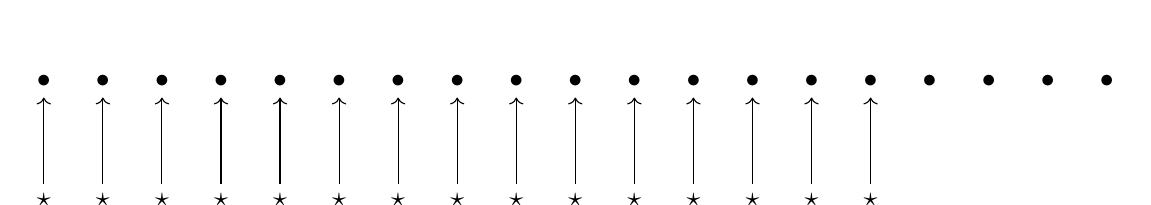
\begin{tikzpicture}
\foreach \x in {1,2,3,4,5,6,7,8,9,10,11,12,13,14,15,16,17,18,19}
  \node at (0.75*\x, 1.5) {$\bullet$};

\foreach \x in {1,2,3,4,5,6,7,8,9,10,11,12,13,14,15}
  \node at (0.75*\x, 0) {$\star$};

\foreach \x in {1,2,3,4,5,6,7,8,9,10,11,12,13,14,15}
  \draw [->] (0.75*\x, 0.2) -- (0.75*\x, 1.3);
\end{tikzpicture}}
\end{center}

It is a property of this function---called \textit{injectivity}---that allows us to deduce that there are more dots than stars.

Intuitively, a function $f : X \to Y$ is injective if it puts the elements of $X$ in one-to-one correspondence with the elements of a subset of $Y$---just like how the stars are in one-to-one correspondence with a subset of the dots in the example above.

\begin{definition}
\label{defInjective}\label{defInjection}
\index{function!injective (one-to-one)}
\index{injection}
A function $f : X \to Y$ is \textbf{injective} (or \textbf{one-to-one}) if
\[ \forall a,b \in X,\, f(a) = f(b) \Rightarrow a=b \]
An injective function is said to be an \textbf{injection}.
\end{definition}

\begin{strategy}[Proving a function is injective]
In order to prove that a function $f : X \to Y$ is injective, it suffices to fix $a,b \in X$, assume that $f(a)=f(b)$, and then derive $a=b$.
\end{strategy}

By contraposition, $f : X \to Y$ being injective is equivalent to saying, for all $a,b \in X$, if $a \ne b$, then $f(a) \ne f(b)$. This is usually less useful for \textit{proving} that a function is injective, but it does provide a good intuition---it says that $f$ sends distinct inputs to distinct outputs.

The following is a very simple example from elementary arithmetic:
\begin{example}
Define $f : \mathbb{Z} \to \mathbb{Z}$ by letting $f(x) = 2n+1$ for all $n \in \mathbb{Z}$. We'll prove that $f$ is injective. Fix $m, n \in \mathbb{Z}$, and assume that $f(m)=f(n)$. By definition of $f$, we have $2m+1=2n+1$. Subtracting $1$ yields $2m=2n$, and dividing by $2$ yields $m=n$. Hence $f$ is injective.
\end{example}

The following example is slightly more sophisticated.

\begin{proposition}
\label{propCompositeOfInjectionsIsInjection}
Let $f : X \to Y$ and $g : Y \to Z$ be functions. If $f$ and $g$ are injective, then $g \circ f$ is injective.
\end{proposition}
\begin{cproof}
Suppose that $f$ and $g$ are injective and
%% BEGIN EXTRACT (xtrVariableIntroductionExample) %%
let $a,b \in X$.
We need to prove that
\[ (g \circ f)(a) = (g \circ f)(b) \quad \Rightarrow \quad a=b \]
%% END EXTRACT %%
So assume $(g \circ f)(a) = (g \circ f)(b)$. By definition of function composition, this implies that $g(f(a))=g(f(b))$. By injectivity of $g$, we have $f(a)=f(b)$; and by injectivity of $f$, we have $a=b$.
\end{cproof}

\begin{exercise}
Let $f : X \to Y$ and $g : Y \to Z$ be functions. Prove that if $g \circ f$ is injective, then $f$ is injective.
\end{exercise}

\begin{exercise}
Write out what it means to say a function $f : X \to Y$ is \textit{not} injective, and say how you would prove that a given function is not injective. Give an example of a function which is not injective, and use your proof technique to write a proof that it is not injective.
\end{exercise}

\begin{exercise}
For each of the following functions, determine whether it is injective or not injective.
\begin{itemize} 
\item $f : \mathbb{N} \to \mathbb{Z}$, defined by $f(n)=n^2$ for all $n \in \mathbb{N}$.
\item $g : \mathbb{Z} \to \mathbb{N}$, defined by $g(n)=n^2$ for all $n \in \mathbb{Z}$.
\item $h : \mathbb{N} \times \mathbb{N} \times \mathbb{N} \to \mathbb{N}$, defined by $h(x,y,z) = 2^x \cdot 3^y \cdot 5^z$ for all $x,y,z \in \mathbb{N}$.
\end{itemize}
\end{exercise}

\begin{exercise}
\label{exLinearPolynomialIsInjective}
Let $a,b \in \mathbb{R}$ with $b \ne 0$, and define $f : \mathbb{R} \to \mathbb{R}$ by $f(t) = a+bt$ for all $t \in \mathbb{R}$. Prove that $f$ is injective.
\end{exercise}

\subsection*{Surjectivity}

Let's revisit the rows of dots and stars that we saw earlier.  Beforehand, we made our idea that there are more dots than stars formal by proving the existence of an injection $f : S \to D$ from the set $S$ of stars to the set $D$ of dots.

However, we could have drawn the same conclusion instead from defining a function $D \to S$, which in some sense \textit{covers} the stars with dots---that is, every star is paired up with at least one dot.

\begin{center}
\fitwidth{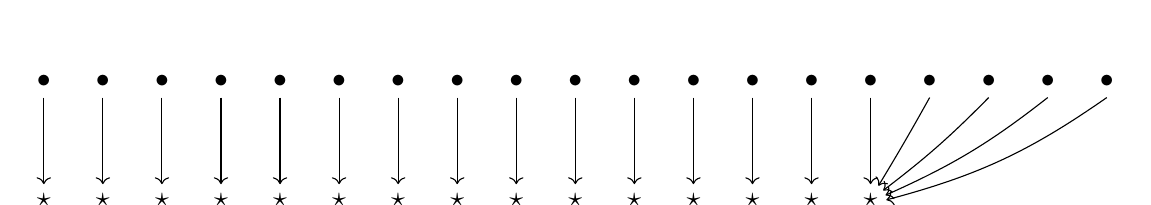
\begin{tikzpicture}
\foreach \x in {1,2,3,4,5,6,7,8,9,10,11,12,13,14,15,16,17,18,19}
  \node at (0.75*\x, 1.5) {$\bullet$};

\foreach \x in {1,2,3,4,5,6,7,8,9,10,11,12,13,14,15}
  \draw [->] (0.75*\x, 1.3) -- (0.75*\x, 0.2);

  \draw [->] (12, 1.3) to [bend left=1] (11.35, 0.18);
  \draw [->] (12.75, 1.3) to [bend left=4] (11.41, 0.12);
  \draw [->] (13.5, 1.3) to [bend left=7] (11.44, 0.06);
  \draw [->] (14.25, 1.3) to [bend left=10] (11.45, 0);

\foreach \x in {1,2,3,4,5,6,7,8,9,10,11,12,13,14,15}
  \node at (0.75*\x, 0) {$\star$};
\end{tikzpicture}}
\end{center}

This property is called \textit{surjectivity}---a function $f : X \to Y$ is surjective if every element of $Y$ is a value of $f$. This is made precise in \Cref{defSurjective}.

\begin{definition}
\label{defSurjective}\label{defSurjection}
A function $f : X \to Y$ is \textbf{surjective}\index{function!surjective}\index{surjection} (or \textbf{onto}) if
\[ \forall y \in Y,\ \exists x \in X,\ f(x) = y \]
A surjective function is said to be a \textbf{surjection}.
\end{definition}

\begin{strategy}
To prove that a function $f : X \to Y$ is surjective, it suffices to take an arbitrary element $y \in Y$ and, in terms of $y$, find an element $x \in X$ such that $f(x)=y$.

In order to find $x$, it is often useful to start from the equation $f(x)=y$ and derive some possible values of $x$. But be careful---in order to complete the proof, it is necessary to verify that the equation $f(x)=y$ is true for the chosen value of $x$.
\end{strategy}

\begin{example}
Fix $n \in \mathbb{N}$ with $n > 0$, and define a function $r : \mathbb{Z} \to \{ 0, 1, \dots, n-1 \}$ by letting $r(a)$ be the remainder of $a$ when divided by $n$ (see \Cref{thmDivisionPreliminary}). This function is surjective, since for each $k \in \{ 0, 1, \dots, n-1 \}$ we have $r(k)=k$.
\end{example}

\begin{exercise}
For each of the following pairs of sets $(X,Y)$, determine whether the function $f : X \to Y$ defined by $f(x)=2x+1$ is surjective.
\begin{enumerate}[(a)]
\item $X = \mathbb{Z}$ and $Y = \{ x \in \mathbb{Z} \mid x \text{ is odd} \}$;
\item $X = \mathbb{Z}$ and $Y = \mathbb{Z}$;
\item $X = \mathbb{Q}$ and $Y = \mathbb{Q}$;
\item $X = \mathbb{R}$ and $Y = \mathbb{R}$.
\end{enumerate}
\end{exercise}

\begin{exercise}
Let $f : X \to Y$ be a function. Find a subset $V \subseteq Y$ and a surjection $g : X \to V$ agreeing with $f$ (that is, such that $g(x)=f(x)$ for all $x \in X$).
\hintlabel{exSurjectiveCorestriction}{%
Recall \Cref{defImage}.
}
\end{exercise}

\begin{exercise}
Let $f : X \to Y$ be a function. Prove that $f$ is surjective if and only if $Y=f[X]$
\end{exercise}

\begin{exercise}
\label{exEpiMonoFactorisation}
Let $f : X \to Y$ be a function. Prove that there is a set $Z$ and functions
\[ p : X \to Z \quad \text{and} \quad i : Z \to Y \]
such that $p$ is surjective, $i$ is injective, and $f = i \circ p$.
\begin{backhint}
\hintref{exEpiMonoFactorisation}
If $Z$ were a subset of $Y$, then we could easily define an injection $i : Z \to Y$ by $i(z)=z$ for all $z \in Z$. Are there any subsets of $Y$ that are associated with a function whose codomain is $Y$?
\end{backhint}
\end{exercise}

\begin{exercise}
Let $f : X \to \mathcal{P}(X)$ be a function. By considering the set $B = \{ x \in X \mid x \not\in f(x) \}$, prove that $f$ is not surjective.
\hintlabel{exRussellSubset}{%
Note that $B \in \mathcal{P}(X)$. Prove that there does not exist $a \in X$ such that $B = f(a)$.
}
\end{exercise}

\subsection*{Bijectivity}

Bijective functions formalise the idea of putting sets into one-to-one correspondence---each element of one set is paired with exactly one element of another.

\begin{definition}
\label{defBijective}\label{defBijection}
A function $f : X \to Y$ is \textbf{bijective}\index{function!bijective} if it is injective and surjective. A bijective function is said to be a \textbf{bijection}\index{bijection}.
\end{definition}

\begin{prooftip}
To prove that a function $f$ is bijective, prove that it is injective and surjective.
\end{prooftip}

\begin{example}
\label{exDyadicRationalsBijection}
Let $D \subseteq \mathbb{Q}$ be the set of \textit{dyadic rational numbers}, that is
\[ D = \left\{ x \in \mathbb{Q} \ \bigg|\  x = \frac{a}{2^n} \text{ for some } a \in \mathbb{Z} \text{ and } n \in \mathbb{N} \right\} \]
Let $k \in \mathbb{N}$, and define $f : D \to D$ by $f(x)=\frac{x}{2^k}$. We will prove that $f$ is a bijection.
\begin{itemize}
\item (\textbf{Injectivity}) Fix $x,y \in D$ and suppose that $f(x)=f(y)$. Then $\frac{x}{2^k}=\frac{y}{2^k}$, so that $x=y$, as required.
\item (\textbf{Surjectivity}) Fix $y \in D$. We need to find $x \in D$ such that $f(x)=y$. Well certainly if $2^ky \in D$ then we have \[ f(2^ky)=\frac{2^ky}{2^k}=y \]
so it suffices to prove that $2^ky \in D$.
%% BEGIN EXTRACT (xtrCasesExample)
Since $y \in D$, we must have $y=\frac{a}{2^n}$ for some $n \in \mathbb{N}$.
\begin{itemize}
\item If $k \le n$ then $n-k \in \mathbb{N}$ and so $2^ky=\frac{a}{2^{n-k}} \in D$.
\item If $k > n$ then $k-n>0$ and $2^ky = 2^{k-n}a \in \mathbb{Z}$; but $\mathbb{Z} \subseteq D$ since if $a \in \mathbb{Z}$ then $a=\frac{a}{2^0}$. So again we have $2^ky \in D$.
\end{itemize}
In both cases we have $2^ky \in D$; and $f(2^ky)=y$, so that $f$ is surjective.
%% END EXTRACT
\end{itemize}
Since $f$ is both injective and surjective, it is bijective.
\end{example}

\begin{exercise}
\label{exIdentityBijection}
Let $X$ be a set. Prove that the identity function $\mathrm{id}_X : X \to X$ is a bijection.
\end{exercise}

\begin{exercise}
\label{exCompositeOfBijectionsIsBijection}
Let $f : X \to Y$ and $g : Y \to Z$ be bijections. Prove that $g \circ f$ is a bijection.
\end{exercise}

\subsection*{Inverses}

Our next goal is to characterise injections, surjections and bijections in terms of other functions, called \textit{inverses}.

Recall \Cref{defInjection}, which says that a function $f : X \to Y$ is injective if, for all $a,b \in X$, if $f(a)=f(b)$ then $a=b$.

\begin{exercise}
Let $f : X \to Y$ be a function. Prove that $f$ is injective if and only if
\[ \forall y \in f[X],\, \exists ! x \in X,\, y=f(x) \]
\end{exercise}

Thinking back to \Cref{secFunctions}, you might notice that this means that the logical formula `$y=f(x)$' defines a function $f[X] \to X$---specifically, if $f$ is injective then there is a function $g : f[X] \to X$ which is (well-)defined by specifying $x=g(f(x))$ for all $x \in X$. Thinking of $f$ as an \textit{encoding} function, we then have that $g$ is the corresponding \textit{decoding} function---decoding is possible by injectivity of $f$. (If $f$ were not injective then distinct elements of $X$ might have the same encoding, in which case we're stuck if we try to decode them!)

\begin{exercise}
\label{exEncodingPairs}
Define a function $e : \mathbb{N} \times \mathbb{N} \to \mathbb{N}$ by $e(m,n) = 2^m \cdot 3^n$. Prove that $e$ is injective. We can think of $e$ as encoding \textit{pairs} of natural numbers as single natural numbers---for example, the pair $(4,1)$ is encoded as $2^4 \cdot 3^1 = 48$. For each of the following natural numbers $k$, find the pairs of natural numbers encoded by $e$ as $k$:
\[ 1 \qquad 24 \qquad 7776 \qquad 59049 \qquad 396718580736 \]
\end{exercise}

In \Cref{exEncodingPairs}, we were able to decode any natural number of the form $2^m \cdot 3^n$ for $m,n \in \mathbb{N}$. This process of decoding yields a function
\[ d : \{ k \in \mathbb{N} \mid k=2^m \cdot 3^n \text{ for some } m,n \in \mathbb{N} \} \to \mathbb{N} \times \mathbb{N} \]
What would happen if we tried to decode a natural number not of the form $2^m \cdot 3^n$ for $m,n \in \mathbb{N}$, say $5$ or $100$? Well\dots{} it doesn't really matter! All we need to be true is that $d(e(m,n))=(m,n)$ for all $(m,n) \in \mathbb{N} \times \mathbb{N}$; the value of $d$ on other natural numbers is irrelevant.

\begin{definition}
\label{defLeftInverse}
\index{inverse!left inverse}
\index{left inverse}
Let $f : X \to Y$ be a function. A \textbf{left inverse} (or \textbf{post-inverse}) for $f$ is a function $g : Y \to X$ such that $g \circ f = \mathrm{id}_X$.
\end{definition}

\begin{example}
Let $e : \mathbb{N} \times \mathbb{N} \to \mathbb{N}$ be as in \Cref{exEncodingPairs}. Define a function $d : \mathbb{N} \to \mathbb{N} \times \mathbb{N}$ by
\[ d(k) = \begin{cases}
(m,n) & \text{if } k=2^m \cdot 3^n \text{ for some } m,n \in \mathbb{N} \\
(0,0) & \text{otherwise}
\end{cases} \]
Note that $d$ is well-defined by the fundamental theorem of arithmetic (\Cref{thmFTA}). Moreover, given $m,n \in \mathbb{N}$, we have
\[ d(e(m,n)) = d(2^m \cdot 3^n) = (m,n) \]
and so $d$ is a left inverse for $e$.
\end{example}

\begin{exercise}
\label{exIfHasLeftInverseThenInjective}
Let $f : X \to Y$ be a function. Prove that if $f$ has a left inverse, then $f$ is injective.
\end{exercise}

\Cref{exIfHasLeftInverseThenInjective} gives us a new strategy for proving that a function is injective.

\begin{strategy}[Proving a function is injective by finding a left inverse]
In order to prove that a function $f : X \to Y$ is injective, it suffices to find a function $g : Y \to X$ such that $g(f(x)) = x$ for all $x \in X$.
\end{strategy}

It would be convenient if the converse to \Cref{exIfHasLeftInverseThenInjective} were true---and it is, provided that we impose the condition that the domain of the function be inhabited.

\begin{proposition}
\label{propIfInjectiveThenHasLeftInverse}
Let $f : X \to Y$ be a function. If $f$ is injective and $X$ is inhabited, then $f$ has a left inverse.
\end{proposition}

\begin{cproof}
Suppose that $f$ is injective and $X$ is inhabited. Fix $x_0 \in X$---note that this element exists since $X$ is inhabited---and define $g : Y \to X$ as follows.
\[ g(y) = \begin{cases} x & \text{if } y=f(x) \text{ for some } x \in X \\ x_0 & \text{otherwise} \end{cases} \]
The only part of the specification of $g$ that might cause it to fail to be well-defined is the case when $y=f(x)$ for some $x \in X$. The reason why $g$ is well-defined is precisely injectivity of $f$: if $y=f(x)$ for some $x \in X$, then the value of $x \in X$ for which $y = f(x)$ is unique. (Indeed, if $a \in X$ satisfied $y=f(a)$, then we'd have $a=x$ by injectivity of $f$.)

So $g$ is indeed well-defined. To see that $g$ is a left inverse for $f$, let $x \in X$. Letting $y = f(x)$, we see that $y$ falls into the first case in the specification of $g$, so that $g(f(x)) = g(y) = a$ for the value of $a \in X$ for which $y = f(a)$---but as noted above, we have $a=x$ by injectivity of $f$.
\end{cproof}

\begin{exercise}
Let $f : X \to Y$ be a function with left inverse $g : Y \to X$. Prove that $g$ is a surjection.
\hintlabel{exLeftInversesAreSurjective}{%
This can be proved in a single sentence; if you find yourself writing a long proof, then there is an easier way.
}
\end{exercise}

We established a relationship between injections and left inverses in \Cref{exIfHasLeftInverseThenInjective,propIfInjectiveThenHasLeftInverse}, so it might come as no surprise that there is a relationship between surjections and \textit{right} inverses.

\begin{definition}
\label{defRightInverse}
\index{inverse!right inverse}
\index{right inverse}
Let $f : X \to Y$ be a function. A \textbf{right inverse} (or \textbf{pre-inverse}) for $f$ is a function $g : Y \to X$ such that $f \circ g = \mathrm{id}_Y$.
\end{definition}

\begin{example}
Define $f : \mathbb{R} \to \mathbb{R}^{\ge 0}$ by $f(x)=x^2$. Note that $f$ is surjective, since for each $y \in \mathbb{R}^{\ge 0}$ we have $\sqrt{y} \in \mathbb{R}$ and $f(\sqrt{y}) = y$. However $f$ is not injective; for instance
\[ f(-1) = 1 = f(1) \]
Here are three right inverses for $f$:
\begin{itemize}
\item The positive square root function $g : \mathbb{R}^{\ge 0} \to \mathbb{R}$ defined by $g(y)=\sqrt{y}$ for all $y \in \mathbb{R}^{\ge 0}$. Indeed, for each $y \in \mathbb{R}^{\ge 0}$ we have
\[ f(g(y)) = f(\sqrt{y}) = (\sqrt{y})^2 = y \]
\item The negative square root function $h : \mathbb{R}^{\ge 0} \to \mathbb{R}$ defined by $h(y)=-\sqrt{y}$ for all $y \in \mathbb{R}^{\ge 0}$. Indeed, for each $y \in \mathbb{R}^{\ge 0}$ we have
\[ f(h(y)) = f(-\sqrt{y}) = (-\sqrt{y})^2 = y \]
\item The function $k : \mathbb{R}^{\ge 0} \to \mathbb{R}$ defined by
\[ k(y) = \begin{cases}
\sqrt{y} & \text{if } 2n \le y < 2n+1 \text{ for some } n \in \mathbb{N} \\
-\sqrt{y} & \text{otherwise}
\end{cases} \]
Note that $k$ is well-defined, and again $f(k(y)) = y$ for all $y \in \mathbb{R}^{\ge 0}$ since no matter what value $k(y)$ takes, it is equal to either $\sqrt{y}$ or $-\sqrt{y}$.
\end{itemize}
There are many more right inverses for $f$---in fact, there are infinitely many more!
\end{example}

\begin{exercise}
Let $f : X \to Y$ be a function. Prove that if $f$ has a right inverse, then $f$ is surjective.
\hintlabel{exIfHasRightInverseThenSurjective}{%
The proof is almost identical to \Cref{exLeftInversesAreSurjective}.
}
\end{exercise}

\begin{strategy}[Proving a function is surjective by finding a right inverse]
In order to prove that a function $f : X \to Y$ is surjective, it suffices to find a function $g : Y \to X$ such that $f(g(y)) = y$ for all $y \in Y$.
\end{strategy}

\subsection*{Interlude: the axiom of choice}

It would be convenient if the converse to \Cref{exIfHasRightInverseThenSurjective} were true---that is, if $f : X \to Y$ is surjective, then it has a right inverse. Let's examine what a proof of this fact would entail. The fact that $f : X \to Y$ is surjective can be expressed as
\[ \forall y \in Y,\, \exists x \in X,\, f(x) = y \]
A right inverse would be a function $g : Y \to X$, so by \Cref{defFunction}, it must satisfy the following condition
\[ \forall y \in Y,\, \exists ! x \in X,\, g(y) = x \]

The temptation is therefore to construct $g : Y \to X$ as follows. Let $y \in Y$. By definition of surjectivity, there exists some $x \in X$ such that $f(x) = y$---define $g(y)$ to be such an element $x$. Then we have $f(g(y)) = f(x) = y$, as required.

There is an extremely subtle---but important---issue with this construction.

By choosing $g(y)$ to be a fixed element of $X$ such that $f(x) = y$, we are assuming ahead of time that there is a mechanism for choosing, for each $y \in Y$, a unique element of $f^{-1}[\{y\}]$ to be the value of $g(y)$. In other words we are assuming that some statement $R(x,y)$ satisfies the property
\[ \forall y \in Y,\, \exists ! x \in X,\, [x \in f^{-1}[\{y\}] \wedge R(x,y)] \]
But by \Cref{defFunction}, this assumption is saying exactly that there exists a function $Y \to X$ that associates to each $y \in Y$ an element $x \in X$ such that $f(x) = y$.

To state this in plainer terms: we tried to prove that there exists a right inverse for $f$ by assuming that there exists a right inverse for $f$. Evidently, this is not a valid proof strategy.

Surprisingly, it turns out that neither the assumption that every surjection has a right inverse, nor the assumption that there exists a surjection with no right inverse, leads to a contradiction. As such, the assertion that every surjection has a right inverse is \textit{provably unprovable}, although the proof that it is unprovable is far beyond the scope of this textbook.

Nonetheless, the construction of a right inverse that we gave above didn't \textit{feel} like we were abusing the fabric of mathematics and logic.

The essence of the proof is that if a statement of the form $\forall a \in A,\, \exists b \in B,\, p(a,b)$ is true, then we should be able to define a function $h : A \to B$ such that $p(a,h(a))$ is true for all $a \in A$: the function $h$ `chooses' for each $a \in A$ a particular element $b = h(a) \in B$ such that $p(a,b)$ is true.

What makes this possible is to \textit{axiom of choice}, stated precisely below.

\begin{axiom}[Axiom of choice]
\label{axChoice}
\index{axiom of choice}
Let $\{ X_i \mid i \in I \}$ be a family of inhabited sets. Then there is a function $h : I \to \bigcup\limits_{i \in I} X_i$ such that $h(i) \in X_i$ for each $i \in I$.
\end{axiom}

There are reasons to keep track of the axiom of choice:
\begin{itemize}
\item The axiom of choice is perhaps the \textit{strangest} assumption that we make---most of the other axioms that we have stated have been `evidently true', but this is not the case for the axiom of choice;
\item There are fields of mathematics which require the translation of results about sets into results about other kinds of objects---knowing whether the axiom of choice is necessary to prove a result tells us whether this is possible;
\item The axiom of choice is highly non-constructive: if a proof of a result that does not use the axiom of choice is available, it usually provides more information than a proof of the same result that does use the axiom of choice.
\end{itemize}

With this in mind, when we need to invoke the axiom of choice to prove a result, we will mark the result with the letters {\small \textbf{AC}}. This can be freely ignored on first reading, but readers may find it useful when using this book as a reference at a later date.

\begin{propositionac}
\label{propUsingAC}
Let $X$ and $Y$ be sets and let $p(x,y)$ be a logical formula with free variables $x \in X$ and $y \in Y$. If $\forall x \in X,\, \forall y \in Y,\, p(x,y)$ is true, then there exists a function $h : X \to Y$ such that $\forall x \in X,\, p(x,h(x))$ is true.
\end{propositionac}

\begin{cproof}
For each $a \in X$, define $Y_a = \{ b \in Y \mid p(a,b) \}$. Note that $Y_a$ is inhabited for each $a \in X$ by the assumption that $\forall x \in X,\, \exists y \in Y,\, p(x,y)$ is true. Since $Y_a \subseteq Y$ for each $a \in X$, by the axiom of choice there exists a function $h : X \to Y$ such that $h(a) \in Y_a$ for all $a \in X$. But then $p(a,h(a))$ is true for each $a \in X$ by definition of the sets $Y_a$.
\end{cproof}

In light of \Cref{propUsingAC}, the axiom of choice manifests itself in proofs as the following proof strategy.

\begin{strategyac}[Making choices]
\label{strUsingAC}
If an assumption in a proof has the form $\forall x \in X,\, \exists y \in Y,\, p(x,y)$, then we may make a choice, for each $a \in A$, of a particular element $b = b_a \in B$ for which $p(a,b)$ is true.
\end{strategyac}

\subsection*{Back to inverses}

We now return to the converse of \Cref{exIfHasRightInverseThenSurjective}.

\begin{propositionac}
Every surjection has a right inverse.
\end{propositionac}

\begin{cproof}
Let $f : X \to Y$ be a surjection, and define $g : Y \to X$ as follows. Given $y \in Y$, define $g(y)$ to be a particular choice of $x \in X$ such that $f(x) = y$---note that there exists such an element $x \in X$ since $f$ is surjective, so $g$ exists by \Cref{strUsingAC}. But then by definition of $g$ we have $f(g(y)) = y$ for all $y \in Y$, so that $g$ is a surjection.
\end{cproof}

It seems logical that we might be able to classify bijections as being those functions which have a left inverse and a right inverse. We can actually say something stronger---the left and right inverse can be taken to be the same function! (In fact, \Cref{propLeftAndRightInversesAreEqual} establishes that they are necessarily the same function.)

\begin{definition}
\label{defInverse}
\index{inverse!two-sided}
\index{two-sided inverse}
Let $f : X \to Y$ be a function. A (\textbf{two-sided}) \textbf{inverse} for $f$ is a function $g : Y \to X$ which is both a left inverse and a right inverse for $f$.
\end{definition}

It is customary to simply say `inverse' rather than `two-sided inverse'.

\begin{example}
Let $D$ be the set of dyadic rational numbers, as defined in \Cref{exDyadicRationalsBijection}. There, we defined a function $f : D \to D$ defined by $f(x)=\frac{x}{2^k}$ for all $x \in D$, where $k$ is some fixed natural number. We find an inverse for $f$.

Define $g : D \to D$ by $g(x) = 2^kx$. Then
\begin{itemize}
\item $g$ is a left inverse for $f$. To see this, note that for all $x \in D$ we have
\[ g(f(x)) = g(\frac{x}{2^k}) = 2^k \cdot \frac{x}{2^k} = x \]
\item $g$ is a right inverse for $f$. To see this, note that for all $y \in D$ we have
\[ f(g(y)) = f(2^ky) = \frac{2^ky}{2^k} = y \]
\end{itemize}
Since $g$ is a left inverse for $f$ and a right inverse for $f$, it is a two-sided inverse for $f$.
\end{example}

\begin{exercise}
\label{exFindTwoSidedInverses}
The following functions have two-sided inverses. For each, find its inverse and prove that it is indeed an inverse.
\begin{enumerate}[(a)]
\item $f : \mathbb{R} \to \mathbb{R}$ defined by $f(x)=\frac{2x+1}{3}$.
\item $g : \mathcal{P}(\mathbb{N}) \to \mathcal{P}(\mathbb{N})$ defined by $g(X) = \mathbb{N} \setminus X$.
\item $h : \mathbb{N} \times \mathbb{N} \to \mathbb{N}$ defined by $h(m,n) = 2^m(2n+1)-1$ for all $m,n \in \mathbb{N}$.
\end{enumerate}
\begin{backhint}
\hintref{exFindTwoSidedInverses}
For part (c), don't try to write a formula for the inverse of $h$; instead, use the fundamental theorem of arithmetic.
\end{backhint}
\end{exercise}

In light of the correspondences between injections and left inverses, and surjections and right inverses, it may be unsurprising that there is a correspondence between \textit{bijections} and \textit{two-sided inverses}.

\begin{exercise}
\label{exBijectiveIffHasInverse}
Let $f : X \to Y$ be a function. Then $f$ is bijective if and only if $f$ has an inverse.
\end{exercise}

\begin{strategy}[Proving a function is bijective by finding an inverse]
In order to prove that a function $f : X \to Y$ is bijective, it suffices to find a function $g : Y \to X$ such that $g(f(x)) = x$ for all $x \in X$ and $f(g(y)) = y$ for all $y \in Y$.
\end{strategy}

When proving a function $f : X \to Y$ is bijective by finding an inverse $g : Y \to X$, it is important to check that $g$ is \textit{both} a left inverse \textit{and} a right inverse for $f$. If you only prove that $g$ is a left inverse for $f$, for example, then you have only proved that $f$ is injective!

It turns out that if a function has both a left and a right inverse, then they must be equal. This is the content of the following proposition.

\begin{proposition}
\label{propLeftAndRightInversesAreEqual}
Let $f : X \to Y$ be a function and suppose $\ell : Y \to X$ is a left inverse for $f$ and $r : Y \to X$ is a right inverse for $f$. Then $\ell=r$.
\end{proposition}
\begin{cproof}
The proof is deceptively simple:
\begin{align*}
\ell &= \ell \circ \mathrm{id}_Y && \text{by definition of identity functions} \\
&= \ell \circ (f \circ r) && \text{since $r$ is a right inverse for $f$} \\
&= (\ell \circ f) \circ r && \text{by \Cref{exCompositionIsAssociative}} \\
&= \mathrm{id}_X \circ r && \text{since $\ell$ is a left inverse for $f$} \\
&= r && \text{by definition of identity functions}
\end{align*}
\end{cproof}

There is some intuition behind why the left and right inverses of a function $f : X \to Y$ should be equal if they both exist.
\begin{itemize}
\item A left inverse $\ell : Y \to X$ exists only if $f$ is injective. It looks at each element $y \in Y$ and, if it is in the image of $f$, returns the (unique) value $x \in X$ for which $f(x)=y$.
\item A right inverse $r : Y \to X$ exists only if $f$ is surjective. It looks at each element $y \in Y$ and picks out one of the (possibly many) values $x \in X$ for which $f(x)=y$.
\end{itemize}
When $f$ is a bijection, every element of $Y$ is in the image of $f$ (by surjectivity), and is a value of $f$ at a unique element of $X$ (by injectivity), and so the left and right inverses are forced to return the same value on each input---hence they are equal.

It follows from \Cref{propLeftAndRightInversesAreEqual} that, for any function $f : X \to Y$, any two inverses for $f$ are equal---that is, every bijective function has a \textit{unique} inverse!

\begin{notation}
Let $f : X \to Y$ be a function. Write $f^{-1} : Y \to X$\nindex{functionInverse}{$f^{-1}$}{inverse function} to denote the (unique) inverse for $f$, if it exists.
\end{notation}

\begin{proposition}
Let $f : X \to Y$ be a bijection. A function $g : Y \to X$ is a left inverse for $f$ if and only if it is a right inverse for $f$.
\end{proposition}

\begin{cproof}
We will prove the two directions separately.
\begin{itemize}
\item ($\Rightarrow$) Suppose $g : Y \to X$ is a left inverse for $f$---that is, $g(f(x))=x$ for all $x \in X$. We prove that $f(g(y))=y$ for all $y \in Y$, thus establishing that $g$ is a right inverse for $f$. So let $y \in Y$. Since $f$ is a bijection, it is in particular a surjection, so there exists $x \in X$ such that $y=f(x)$. But then
\begin{align*}
f(g(y)) &= f(g(f(x))) && \text{since $y=f(x)$} \\
&= f(x) && \text{since $g(f(x))=x$} \\
&= y && \text{since $y=f(x)$}
\end{align*}
So indeed $g$ is a right inverse for $f$.
\item ($\Leftarrow$) Suppose $g : Y \to X$ is a right inverse for $f$---that is, $f(g(y))=y$ for all $y \in Y$. We prove that $g(f(x))=x$ for all $x \in X$, thus establishing that $g$ is a left inverse for $f$. So let $x \in X$. Letting $y = f(x)$, we have $f(g(y)) = y$ since $g$ is a right inverse for $f$. This says precisely that $f(g(f(x)) = f(x)$, since $y=f(x)$. By injectivity of $f$, we have $g(f(x))=x$, as required.
\end{itemize}
\end{cproof}

\begin{exercise}
\label{exInverseBijection}
Let $f : X \to Y$ be a bijection. Prove that $f^{-1} : Y \to X$ is a bijection.
\begin{backhint}
\hintref{exInverseBijection}
Use \Cref{exBijectiveIffHasInverse}.
\end{backhint}
\end{exercise}

\begin{exercise}
\label{exCompositeBijection}
Let $f : X \to Y$ and $g : Y \to Z$ be bijections. Prove that $g \circ f : X \to Z$ is a bijection, and write an expression for its inverse in terms of $f^{-1}$ and $g^{-1}$.
\end{exercise}

\begin{exercise}
Let $f : X \to A$ and $g : Y \to B$ be bijections. Prove that there is a bijection $X \times Y \to A \times B$, and describe its inverse.
\hintlabel{exCartesianProductOfBijections}{%
Define $h : X \times Y \to A \times B$ by $h(x,y) = (f(x), g(y))$ for all $x \in X$ and all $y \in Y$; find an inverse for $h$ in terms of the inverses of $f$ and $g$.
}
\end{exercise}

At the beginning of this section we motivated the definitions of injections, surjections and bijections by using them to compare two quantities (of dots and stars)---however, as you might have noticed, we have not yet actually proved that thais intuition aligns with reality. For example, how do we know that if there is an injection $f : X \to Y$ then $Y$ has at least as many elements as $X$?

Answering this seemingly simple question is surprisingly difficult and has different answers depending on whether the sets involved are finite or infinite. In fact, the words `finite', `infinite' and `size' are themselves defined in terms of injections, surjections and bijections! We therefore leave this task to future sections.

In \Cref{secFiniteSets}, we define what it means for a set to be finite and what the size of a finite set is (\Cref{defFiniteSet}), and then prove that the sizes of finite sets can be compared by finding an injection, surjection or bijection between them \Cref{thmJectionsAndSizeOfNaturalNumbers}.

Comparing the sizes of infinite sets, and even defining what `size' means for infinite sets, is another can of worms entirely and leads to some fascinating mathematics. For example, we can prove some counterintuitive results, such as the set $\mathbb{N}$ of natural numbers and the set $\mathbb{Q}$ of rational numbers have the same size. The journey down this rabbit hole begins in \Cref{chInfinity}.

\begin{tldr}{secInjectionsSurjections}

\subsubsection*{Injections, surjections and bijections}

\begin{tldrlist}
\tldritem{defInjection} A function $f : X \to Y$ is \textit{injective} if, for all $a,b \in X$, if $f(a)=f(b)$, then $a=b$; this is equivalent to saying that distinct elements of $X$ are mapped by $f$ to distinct elements of $Y$.
\tldritem{defSurjection} A function $f : X \to Y$ is \textit{surjective} if, for all $y \in Y$, there exists $x \in X$ such that $f(x)=y$; this is equivalent to saying that the image of $f$ is its entire codomain.
\tldritem{defBijection} A function $f : X \to Y$ is \textit{bijective} if it is both injective and surjective.
\end{tldrlist}

\subsubsection*{Inverses}

\begin{tldrlist}
\tldritem{defLeftInverse} A \textit{left inverse} for a function $f : X \to Y$ is a function $g : Y \to X$ such that $g \circ f = \mathrm{id}_X$. If $f$ has a left inverse, then it is injective; conversely, if $f$ is injected \textit{and} $X$ is inhabited, then $f$ has a left inverse.
\tldritem{defRightInverse} A \textit{right inverse} for a function $f : X \to Y$ is a function $g : Y \to X$ such that $f \circ g = \mathrm{id}_Y$. If $f$ has a right inverse, then it is surjective; conversely, assuming the axiom of choice, if $f$ is surjective, then it has a right inverse.
\tldritem{defInverse} An \textit{inverse} for a function $f : X \to Y$ is a function $g : Y \to X$ that is both a left inverse and a right inverse for $f$. A function $f$ is bijective if and only if it has an inverse.
\tldritem{propLeftAndRightInversesAreEqual} If a function $f : X \to Y$ has both a left and a right inverse, then they are equal; in particular, every bijection has a unique inverse, denoted by $f^{-1} : Y \to X$.
\end{tldrlist}

\end{tldr}

\index{injection|)}
\index{surjection|)}
\index{bijection|)}

% Chapter exercises
\chexbegin{chFunctions}
% !TeX root = ../../infdesc.tex
\begin{chapex}
For each of the following equations, determine whether there exists a function $f : \mathbb{R} \to \mathbb{R}$ such that, for all $x,y \in \mathbb{R}$, the equation holds if and only if $y=f(x)$.
\begin{multicols}{3}
\begin{enumerate}[(a)]
\item $x+y=1$
\item $x^2+y^2=1$
\item $x=0$
\item $y=0$
\item $(1+x^2)y=1$
\item $(1-x^2)y=0$
\end{enumerate}
\end{multicols}
\end{chapex}

\begin{chapex}
Let $X$ be a set. Prove that
\[ \forall a \in X,\, \exists ! U \in \mathcal{P}(X), (a \in U \wedge \exists ! x \in X,\, x \in U) \]
Give an explicit description of the function $X \to \mathcal{P}(X)$ that is suggested by this logical formula.
\hintlabel{cqSingletonSubsetFunction}{%
}
\end{chapex}

\begin{chapex}
Show that there is only one function whose codomain is empty. What is its domain?
\hintlabel{cqFunctionEmptyCodomain}{%
Given a function $f : X \to \varnothing$, we must have $f(a) \in \varnothing$ for each $a \in X$.
}
\end{chapex}

\begin{definition}
\label{defEvenOddFunction}
\index{even!function}
\index{odd!function}
A function $f : \mathbb{R} \to \mathbb{R}$ is \textbf{even} if $f(-x)=f(x)$ for all $x \in \mathbb{R}$, and it is \textbf{odd} if $f(-x)=-f(x)$ for all $x \in \mathbb{R}$.
\end{definition}

\begin{chapex}
Let $n \in \mathbb{N}$. Prove that the function $f : \mathbb{R} \to \mathbb{R}$ defined by $f(x)=x^n$ for all $x \in \mathbb{R}$ is even if and only if $n$ is even, and odd if and only if $n$ is odd.
\end{chapex}

\begin{chapex}
Prove that there is a unique function $f : \mathbb{R} \to \mathbb{R}$ that is both even and odd.
\end{chapex}

\begin{chapex}
Let $U \subseteq \mathbb{R}$, and let $\chi_U : \mathbb{R} \to \{0,1\}$ be the indicator function of $U$.
\begin{enumerate}[(a)]
\item Prove that $\chi_U$ is an even function if and only if $U = \{ -u \mid u \in U \}$;
\item Prove that $\chi_U$ is an odd function if and only if $\mathbb{R} \setminus U = \{ -u \mid u \in U \}$.
\end{enumerate}
\end{chapex}

\begin{chapex}
Prove that for every function $f : \mathbb{R} \to \mathbb{R}$, there is a unique even function $g : \mathbb{R} \to \mathbb{R}$ and a unique odd function $h : \mathbb{R} \to \mathbb{R}$ such that $f(x)=g(x)+h(x)$ for all $x \in \mathbb{R}$.
\hintlabel{cqEveryFunctionIsUniquelySumOfEvenAndOdd}{%
Consider $f(x)+f(-x)$ and $f(x)-f(-x)$ for $x \in \mathbb{R}$.
}
\end{chapex}

\begin{chapex}
Let $\{ \theta_n : [n] \to [n] \mid n \in \mathbb{N} \}$ be a family of functions such that $f \circ \theta_m = \theta_n \circ f$ for all $f : [m] \to [n]$. Prove that $\theta_n = \mathrm{id}_{[n]}$ for all $n \in \mathbb{N}$.
\hintlabel{cqNaturalTransformationFromIdToId}{%
Fix $n \in \mathbb{N}$ and consider how $\theta_n$ interacts with functions $f : [1] \to [n]$.
}
\end{chapex}

\begin{chapex}
Let $X$ be a set and let $U, V \subseteq X$. Describe the indicator function $\chi_{U \symmdiff V}$ of the symmetric difference of $U$ and $V$ (see \Cref{defSymmetricDifference}) in terms of $\chi_U$ and $\chi_V$.
\end{chapex}

\begin{chapex}
\label{cqAntiderivativeOfLogarithm}
[This question assumes some familiarity with 
integral calculus.] A lie that is commonly told to calculus students is that
\[ \int \dfrac{1}{x} \, dx = \log(|x|) + c \]
where $\log$ denotes the natural logarithm function and $c$ is an arbitrary real constant. Prove that it is actually the case that
\[ \int \dfrac{1}{x} \, dx = \log(|x|) + a \chi_U(x) + b \chi_V(x) \]
where $a$ and $b$ are arbitrary real constants, and $U$ and $V$ are particular (inhabited) subsets of $\mathbb{R} \setminus \{ 0 \}$ that you should determine.
\end{chapex}

\subsection*{Images and preimages}

In \Crefrange{cqComputeImageBegin}{cqComputeImageEnd}, find the image $f[U]$ of the subset $U$ of the domain of the function $f$ described in the question.

\begin{chapex}
\label{cqComputeImageBegin}
$f : \mathbb{R} \to \mathbb{R}$; $f(x) = \sqrt{1+x^2}$ for all $x \in \mathbb{R}$; $U = \mathbb{R}$.
\end{chapex}

\begin{chapex}
$f : \mathbb{Z} \times \mathbb{Z} \to \mathbb{Z}$; $f(a,b) = a+2b$ for all $(a,b) \in \mathbb{Z} \times \mathbb{Z}$; $U = \{ 1 \} \times \mathbb{Z}$.
\end{chapex}

\begin{chapex}
$f : \mathbb{N} \to \mathcal{P}(\mathbb{N})$; $f(0) = \varnothing$ and $f(n+1) = f(n) \cup \{ n \}$ for all $n \in \mathbb{N}$; $U = \mathbb{N}$.
\end{chapex}

\begin{chapex}
$f : \mathbb{R}^{\mathbb{R}} \to \mathbb{R}^{\mathbb{R}}$ (where $\mathbb{R}^{\mathbb{R}}$ is the set of all functions $\mathbb{R} \to \mathbb{R}$); $f(h)(x) = h(|x|)$ for all $h \in \mathbb{R}^{\mathbb{R}}$ and all $x \in \mathbb{R}$; $U = \mathbb{R}^{\mathbb{R}}$.
\hintlabel{cqComputeImageEnd}{%
Begin by observing that each $h \in f[\mathbb{R}^{\mathbb{R}}]$ is an even function, in the sense of \Cref{defEvenOddFunction}.
}
\end{chapex}

In \Crefrange{cqComputePreimageBegin}{cqComputePreimageEnd}, find the preimage $f^{-1}[V]$ of the subset $V$ of the codomain of the function $f$ described in the question.

\begin{chapex}
\label{cqComputePreimageBegin}
$f : \mathbb{R} \to \mathbb{R}$; $f(x) = \sqrt{1+x^2}$ for all $x \in \mathbb{R}$; $V = (-5,5]$.
\end{chapex}

\begin{chapex}
$f : \mathbb{Z} \times \mathbb{Z} \to \mathbb{Z}$; $f(a,b) = a+2b$ for all $(a,b) \in \mathbb{Z} \times \mathbb{Z}$; $V = \{ n \in \mathbb{Z} \mid n \text{ is odd} \}$.
\end{chapex}

\begin{chapex}
\label{cqComputePreimageEnd}
$f : \mathcal{P}(\mathbb{N}) \times \mathcal{P}(\mathbb{N}) \to \mathcal{P}(\mathbb{N})$; $f(A,B) = A \cap B$ for all $(A,B) \in \mathcal{P}(\mathbb{N}) \times \mathcal{P}(\mathbb{N})$; $V = \{ \varnothing \}$.
\end{chapex}

\begin{chapex}
Let $f : X \to Y$ be a function. For each of the following statements, either prove it is true or find a counterexample.
\begin{multicols}{2}
\begin{enumerate}[(a)]
\item $U \subseteq f^{-1}[f[U]]$ for all $U \subseteq X$;
\item $f^{-1}[f[U]] \subseteq U$ for all $U \subseteq X$;
\item $V \subseteq f[f^{-1}[V]]$ for all $V \subseteq Y$;
\item $f[f^{-1}[V]] \subseteq V$ for all $V \subseteq Y$.
\end{enumerate}
\end{multicols}
\end{chapex}

\begin{chapex}
Let $f : X \to Y$ be a function, let $A$ be a set, and let $p : X \to A$ and $i : A \to Y$ be functions such that the following conditions hold:
\begin{enumerate}[(i)]
\item $i$ is injective;
\item $i \circ p = f$; and
\item If $q : X \to B$ and $j : B \to Y$ are functions such that $j$ is injective and $j \circ q = f$, then there is a unique function $u : A \to B$ such that $j \circ u = i$.
\end{enumerate}
Prove that there is a unique bijection $v : A \to f[X]$ such that $i(a)=v(a)$ for all $a \in f[X]$.
\hintlabel{cqUniversalPropertyOfImage}{%
This problem is very fiddly. First prove that conditions (i)--(iii) are satisfied when $A = f[X]$ and $p$ and $i$ are chosen appropriately. Then condition (iii) in each case (for $A$ and for $f[X]$) defines functions $v : A \to f[X]$ and $w : f[X] \to A$, and gives uniqueness of $v$. You can prove that these functions are mutually inverse using the `uniqueness' part of condition (iii).
}
\end{chapex}

\begin{chapex}
Let $f : X \to Y$ be a function and let $U, V \subseteq Y$. Prove that:
\begin{enumerate}[(a)]
\item $f^{-1}[U \cap V] = f^{-1}[U] \cap f^{-1}[V]$;
\item $f^{-1}[U \cup V] = f^{-1}[U] \cup f^{-1}[V]$; and
\item $f^{-1}[Y \setminus U] = X \setminus f^{-1}[U]$.
\end{enumerate}
Thus preimages preserve the basic set operations.
\end{chapex}

\begin{chapex}
Let $f : X \to Y$ and $g : Y \to Z$ be functions.
\begin{enumerate}[(a)]
\item Prove that $(g \circ f)[U] = g[f[U]]$ for all $U \subseteq X$;
\item Prove that $(g \circ f)^{-1}[W] = f^{-1}[g^{-1}[W]]$ for all $W \subseteq Z$.
\end{enumerate}
\end{chapex}

\subsection*{Injections, surjections and bijections}

\begin{chapex}
\begin{enumerate}[(a)]
\item Prove that, for all functions $f : X \to Y$ and $g : Y \to Z$, if $g \circ f$ is bijective, then $f$ is injective and $g$ is surjective.
\item Find an example of a function $f : X \to Y$ and a function $g : Y \to Z$ such that $g \circ f$ is bijective, $f$ is not surjective and $g$ is not injective.
\end{enumerate}
\hintlabel{cqCompositeOfFunctionsIsBijection}{%
Avoid the temptation to prove either part of this question by contradiction. For (a), a short proof is available directly from the definitions of `injection' and `surjection'. For (b), find as simple a counterexample as you can.
}
\end{chapex}

\begin{chapex}
\label{cqInjectionSurjectionBijection}
For each of the following pairs $(U,V)$ of subsets of $\mathbb{R}$, determine whether the specification `$f(x) = x^2-4x+7$ for all $x \in U$' defines a function $f : U \to V$ and, if it does, determine whether $f$ is injective and whether $f$ is surjective.
\begin{multicols}{2}
\begin{enumerate}[(a)]
\item $U = \mathbb{R}$ and $V = \mathbb{R}$;
\item $U = (1, 4)$ and $V = [3, 7)$;
\item $U = [3, 4)$ and $V = [4, 7)$;
\item $U = (3, 4]$ and $V = [4, 7)$;
\item $U = [2, \infty)$ and $V = [3, \infty)$;
\item $U = [2,\infty)$ and $V = \mathbb{R}$.
\end{enumerate}
\end{multicols}
\end{chapex}

\begin{chapex}
For each of the following pairs of sets $X$ and $Y$, find (with proof) a bijection $f : X \to Y$.
\begin{enumerate}[(a)]
\item $X = \mathbb{Z}$ and $Y = \mathbb{N}$;
\item $X = \mathbb{R}$ and $Y = (-1,1)$;
\item $X = [0,1]$ and $Y = (0,1)$;
\item $X = [a,b]$ and $Y = (c,d)$, where $a,b,c,d \in \mathbb{R}$ with $a<b$ and $c<d$.
\end{enumerate}
\end{chapex}

\begin{chapex}
Prove that the function $f : \mathbb{N} \times \mathbb{N} \to \mathbb{N}$ defined by $f(a,b) = \dbinom{a+b+1}{2} + b$ for all $(a,b) \in \mathbb{N} \times \mathbb{N}$ is a bijection.
\hintlabel{cqElementaryBijectionNTimesNToN}{%
Start by proving that $\dbinom{m}{2} < \dbinom{m+1}{2}$ for all $m \ge 1$. Deduce that, for all $n \in \mathbb{N}$, there is a unique natural number $k$ such that $\dbinom{k+1}{2} \le n < \dbinom{k+2}{2}$. Can you see what this has to do with the function $f$?
}
\end{chapex}

\begin{chapex}
Let $e : X \to X$ be a function such that $e \circ e = e$. Prove that there exist a set $Y$ and functions $f : X \to Y$ and $g : Y \to X$ such that $g \circ f = e$ and $f \circ g = \mathrm{id}_Y$.
\hintlabel{exSplitIdempotents}{%
Consider the set of fixed points of $e$---that is, elements $x \in X$ such that $e(x)=x$.
}
\end{chapex}

\subsection*{True--False questions}

\tfquestiontext{cqFunctionsTFBegin}{cqFunctionsTFEnd}

\begin{chapex} % False
\label{cqFunctionsTFBegin}
The set $G = \{ (x,y) \in \mathbb{R} \times \mathbb{R} \mid x^2=y^2 \}$ is the graph of a function.
\end{chapex}

\begin{chapex} % True
The set $G = \{ (x,y) \in \mathbb{Z}\times \mathbb{N} \mid x^2=y^2 \}$ is the graph of a function.
\end{chapex}

\begin{chapex} % False
Every function with empty domain has an empty codomain.
\end{chapex}

\begin{chapex} % True
Every function with empty codomain has an empty domain.
\end{chapex}

\begin{chapex} % False (in general)
The image of a function is a subset of its domain.
\end{chapex}

\begin{chapex} % True
Given a function $f : X \to Y$, the assignment $V \mapsto f^{-1}[V]$ defines a function $\mathcal{P}(Y) \to \mathcal{P}(X)$.
\end{chapex}

\begin{chapex} % True
Let $f$, $g$ and $h$ be composable functions. If $h \circ g \circ f$ is injective, then $g$ is injective.
\end{chapex}

\begin{chapex} % True
\label{cqFunctionsTFEnd}
Every left inverse is surjective and every right inverse is injective.
\end{chapex}

\subsection*{Always--Sometimes--Never questions}

\asnquestiontext{cqFunctionsASNBegin}{cqFunctionsASNEnd}

\begin{chapex} % Always
\label{cqFunctionsASNBegin}
Let $f : X \to Y$ be a function and let $U \subseteq X$. Then there is a function $g : U \to Y$ defined by $g(x) = f(x)$ for all $x \in U$.
\end{chapex}

\begin{chapex} % Sometimes
Let $f : X \to Y$ be a function and let $V \subseteq Y$. Then there is a function $g : X \to V$ defined by $g(x) = f(x)$ for all $x \in X$.
\end{chapex}

\begin{chapex} % Always
Let $X$ be a set. Then there is a unique function $X \to \{ 0 \}$.
\end{chapex}

\begin{chapex} % Sometimes
Let $X$ be a set. Then there is a unique function $X \to \varnothing$.
\end{chapex}

\begin{chapex} % Sometimes
Let $X$ and $Y$ be sets and let $G \subseteq X \times Y$. Then $G$ is the graph of a function $f : X \to Y$.
\end{chapex}

\begin{chapex} % Never
Let $f : \{ 1, 2, 3 \} \to \{ 1, 2 \}$, let $G = \mathrm{Gr}(f)$ and let $G' = \{ (y,x) \mid (x,y) \in G \}$. Then $G'$ is the graph of a function $\{ 1, 2 \} \to \{ 1, 2, 3 \}$.
\end{chapex}

\begin{chapex} % Always
Let $f : X \to Y$ be a function and let $U \subseteq X$ be inhabited. Then $f[U]$ is inhabited.
\end{chapex}

\begin{chapex} % Sometimes
Let $f : X \to Y$ be a function and let $V \subseteq Y$ be inhabited. Then $f^{-1}[V]$ is inhabited.
\end{chapex}

\begin{chapex} % Sometimes
Let $f : \{ 1, 2 \} \to \{ 1, 2, 3 \}$ be a function. Then $f$ is injective.
\end{chapex}

\begin{chapex} % Never
Let $f : \{ 1, 2 \} \to \{ 1, 2, 3 \}$ be a function. Then $f$ is surjective.
\end{chapex}

\begin{chapex} % Always
Let $a,b,c,d \in \mathbb{R}$ and define $f : \mathbb{R}^2 \to \mathbb{R}^2$ by $f(x,y) = (ax+by,cx+dy)$ for all $(x,y) \in \mathbb{R}^2$. Then $f$ is injective if and only if $f$ is surjective.
\hintlabel{cqLinearMapInjectiveIffSurjective}{%
First prove that $f$ is bijective if and only if $ad \ne bc$.
}
\end{chapex}

\begin{chapex} % Sometimes
\label{cqFunctionsASNEnd}
Let $U, V \subseteq \mathbb{R}$ and suppose that $x^2 \in V$ for all $x \in U$. The function $f : U \to V$ defined by $f(x) = x^2$ is injective.
\end{chapex}
\chexend
% !TeX root = ../../infdesc.tex
\chapter{Mathematical induction}
\label{chMathematicalInduction}


% !TeX root = ../../infdesc.tex
\section{Peano's axioms}
\secbegin{secPeanosAxioms}

The purpose of this section is to forget everything we think we know about the natural numbers, and reconstruct our former knowledge (and more!)\ using the following fundamental property:

\begin{center}
\textit{Every natural number can be obtained in a unique way by\\
starting from zero and adding one some finite number of times.}
\end{center}

This is slightly imprecise---it is not clear what is meant by `adding one some finite number of times', for example. Worse still, we are going to define what `finite' means in terms of natural numbers in \Cref{secFiniteSets}, so we'd better not refer to finiteness in our definition of natural numbers!

The following definition captures precisely the properties that we need in order to characterise the idea of $\mathbb{N}$ that we have in our minds. To begin with, $\mathbb{N}$ should be a set. Whatever the elements of this set $\mathbb{N}$ actually \textit{are}, we will think about them as being natural numbers. One of the elements, in particular, should play the role of the natural number $0$---this will be the \textit{zero element} $z \in \mathbb{N}$; and there should be a notion of `adding one'---this will be the \textit{successor function} $s : \mathbb{N} \to \mathbb{N}$. Thus given an element $n \in \mathbb{N}$, though of as a natural number, we think about the element $s(n)$ as the natural number `$n+1$'. Note that this is strictly for the purposes of intuition: we will define `$+$' and `$1$' in terms of $z$ and $s$, not vice versa.

\begin{definition}
\label{defNotionOfNaturalNumbers}
\index{natural numbers!notion of}
\index{Peano's axioms}
A \textbf{notion of natural numbers} is a set $\mathbb{N}$, together with an element $z \in \mathbb{N}$, called a \textbf{zero element}, and a function $s : \mathbb{N} \to \mathbb{N}$ called a \textbf{successor function}, satisfying the following properties:
\begin{enumerate}[(i)]
\item $z \not\in s[\mathbb{N}]$; that is, $z \ne s(n)$ for any $n \in \mathbb{N}$.
\item $s$ is injective; that is, for all $m,n \in \mathbb{N}$, if $s(m) = s(n)$, then $m=n$.
\item $\mathbb{N}$ is generated by $z$ and $s$; that is, for all sets $X$, if $z \in X$ and for all $n \in \mathbb{N}$ we have $n \in X \Rightarrow s(n) \in X$, then $\mathbb{N} \subseteq X$.
\end{enumerate}
The properties (i), (ii) and (iii) are called \textbf{Peano's axioms}.
\end{definition}

Note that \Cref{defNotionOfNaturalNumbers} does not specify what $\mathbb{N}$, $z$ and $s$ actually are; it just specifies the properties that they must satisfy. It turns out that it doesn't really matter what notion of natural numbers we use, since any two notions are essentially the same. We will not worry about the specifics here---that task is left to \Cref{secConstructions}: a particular notion of natural numbers is defined in \Cref{cnsNaturalNumbersVonNeumann}, and the fact that all notions of natural numbers are `essentially the same' is made precise and proved in \Cref{thmNNNUnique}.

We can define all the concepts involving natural numbers that we are familiar with, and prove all the properties that we take for granted, just from the element $z \in \mathbb{N}$ and the successor function $s : \mathbb{N} \to \mathbb{N}$.

For instance, we define `$0$' to mean $z$, define `$1$' to mean $s(z)$, define `$2$' to mean $s(s(z))$, and so on. Thus `$12$' is defined to mean
\[ s(s(s(s(s(s(s(s(s(s(s(s(z)))))))))))) \]

From now on, then, let's write $0$ instead of $z$ for the zero element of $\mathbb{N}$. It would be nice if we could write `$n+1$' instead of $s(n)$, but we must first define what `$+$' means. In order to do this, we need a way of defining expressions involving natural numbers; this is what the \textit{recursion theorem} allows us to do.

\begin{theorem}[Recursion theorem]
\label{thmRecursion}
\index{recursion!recursion theorem}
Let $X$ be a set. For all $a \in X$ and all $h : \mathbb{N} \times X \to X$, there is a unique function $f : \mathbb{N} \to X$ such that $f(0) = a$ and $f(s(n)) = h(n, f(n))$ for all $n \in \mathbb{N}$.
\end{theorem}

\begin{cproof}
Let $a \in X$ and $h : \mathbb{N} \times X \to X$. We prove existence and uniqueness of $f$ separately.

\begin{itemize}
\item Define $f : \mathbb{N} \to X$ by specifying $f(0) = a$ and $f(s(n)) = h(n, f(n))$. Since $h$ is a function and $s$ is injective, existence and uniqueness of $x \in X$ such that $f(n) = x$ is guaranteed, provided that $f(n)$ is defined, so we need only verify totality.

So let $D = \{ n \in \mathbb{N} \mid f(n) \text{ is defined} \}$. Then:

\begin{itemize}
\item $0 \in D$, since $f(0)$ is defined to be equal to $a$.
\item Let $n \in \mathbb{N}$ and suppose $n \in D$. Then $f(n)$ is defined and $f(s(n)) = h(n, f(n))$, so that $f(s(n))$ is defined, and hence $s(n) \in D$.
\end{itemize}

%% BEGIN EXTRACT (xtrConclusionExample) %%
By condition (iii) of \Cref{defNotionOfNaturalNumbers}, we have $\mathbb{N} \subseteq D$, so that $f(n)$ is defined for all $n \in \mathbb{N}$, as required.
%% END EXTRACT %%

\item To see that $f$ is unique, suppose $g : \mathbb{N} \to X$ were another function such that $g(0) = a$ and $g(s(n)) = h(n, g(n))$ for all $n \in \mathbb{N}$.

To see that $f = g$, let $E = \{ n \in \mathbb{N} \mid f(n) = g(n) \}$. Then
\begin{itemize}
\item $0 \in E$, since $f(0) = a = g(0)$.
\item Let $n \in \mathbb{N}$ and suppose that $n \in E$. Then $f(n) = g(n)$, and so
\[ f(s(n)) = h(n,f(n)) = h(n,g(n)) = g(s(n)) \]
and so $s(n) \in E$.
\end{itemize}
Again, condition (iii) of \Cref{defNotionOfNaturalNumbers} is satisfied, so that $\mathbb{N} \subseteq E$. It follows that $f(n) = g(n)$ for all $n \in \mathbb{N}$, and so $f=g$.
\end{itemize}

Thus we have established the existence and uniqueness of a function $f : \mathbb{N} \to X$ such that $f(0) = a$ and $f(s(n)) = h(n, f(n))$ for all $n \in \mathbb{N}$.
\end{cproof}

The recursion theorem allows us to define expressions involving natural numbers \textit{by recursion}; this is \Cref{strDefinitionByRecursion}.

\begin{strategy}[Definition by recursion]
\label{strDefinitionByRecursion}
\index{recursion!definition by recursion}
In order to specify a function $f : \mathbb{N} \to X$, it suffices to define $f(0)$ and, for given $n \in \mathbb{N}$, assume that $f(n)$ has been defined, and define $f(s(n))$ in terms of $n$ and $f(n)$.
\end{strategy}

\begin{example}
We can use recursion to define addition on the natural numbers as follows.

For fixed $m \in \mathbb{N}$, we can define a function $\mathrm{add}_m : \mathbb{N} \to \mathbb{N}$ by recursion by:
\[ \mathrm{add}_m(0) = m \quad \text{and} \quad \mathrm{add}_m(s(n)) = s(\mathrm{add}_m(n)) \text{ for all } n \in \mathbb{N} \]
In more familiar notation, for $m,n \in \mathbb{N}$, define the expression `$m+n$' to mean $\mathrm{add}_m(n)$. Another way of expressing the recursive definition of $\mathrm{add}_m(n)$ is to say that, for each $m \in \mathbb{N}$, we are defining $m+n$ by recursion on $n$ as follows:
\[ m+0 = m \quad \text{and} \quad m+s(n) = s(m+n) \text{ for all } n \in \mathbb{N} \]
\end{example}

We can use the recursive definition of addition to prove familiar equations between numbers. The following proposition is a proof that $2+2=4$. This may seem silly, but notice that the expression `$2+2=4$' is actually shorthand for the following:
\[ \mathrm{add}_{s(s(0))} (s(s(0))) = s(s(s(s(0)))) \]
We must therefore be careful to apply the definitions in its proof.

\begin{proposition}
\label{propTwoPlusTwoEqualsFour}
$2+2=4$
\end{proposition}

\begin{cproof}
We use the recursive definition of addition.
\begin{align*}
2 + 2 &= 2 + s(1) && \text{since $2=s(1)$} \\
&= s(2+1) && \text{by definition of $+$} \\
&= s(2+s(0)) && \text{since $1=s(0)$} \\
&= s(s(2+0)) && \text{by definition of $+$} \\
&= s(s(2)) && \text{by definition of $+$} \\
&= s(3) && \text{since $3=s(2)$} \\
&= 4 && \text{since $4=s(3)$}
\end{align*}
as required.
\end{cproof}

The following result allows us to drop the notation `$s(n)$' and just write `$n+1$' instead.

\begin{proposition}
\label{propSuccessorIsPlusOne}
For all $n \in \mathbb{N}$, we have $s(n) = n+1$.
\end{proposition}

\begin{cproof}
Let $n \in \mathbb{N}$. Then by the recursive definition of addition we have
\[ n+1 = n+s(0) = s(n+0) = s(n) \]
as required.
\end{cproof}

In light of \Cref{propSuccessorIsPlusOne}, we will now abandon the notation $s(n)$, and write $n+1$ instead.

We can define the arithmetic operations of multiplication and exponentiation by recursion, too.

\begin{example}
Fix $m \in \mathbb{N}$. Define $m \cdot n$ for all $n \in \mathbb{N}$ by recursion on $n$ as follows:
\[ m \cdot 0 = 0 \quad \text{and} \quad m \cdot (n+1) = (m \cdot n) + m \text{ for all } n \in \mathbb{N} \]
Formally, what we have done is define a function $\mathrm{mult}_m : \mathbb{N} \to \mathbb{N}$ recursively by $\mathrm{mult}_m(z)=z$ and $\mathrm{mult}_m(s(n)) = \mathrm{add}_{\mathrm{mult}_m(n)}(m)$ for all $n \in \mathbb{N}$. But the definition we provided is easier to understand.
\end{example}

\begin{proposition}
\label{propTwoTimesTwoEqualsFour}
$2 \cdot 2 = 4$
\end{proposition}

\begin{cproof}
We use the recursive definitions of addition and recursion.
\begin{align*}
2 \cdot 2 &= 2 \cdot (1+1) && \text{since $2=1+1$} \\
&= (2 \cdot 1) + 2 && \text{by definition of $\cdot$} \\
&= (2 \cdot (0+1)) + 2 && \text{since $1 = 0 + 1$} \\
&= ((2 \cdot 0) + 2) + 2 && \text{by definition of $\cdot$} \\
&= (0+2) + 2 && \text{by definition of $\cdot$} \\
&= (0+(1+1)) + 2 && \text{since $2=1+1$} \\
&= ((0+1)+1) + 2 && \text{by definition of $+$} \\
&= (1+1) + 2 && \text{since $1=0+1$} \\
&= 2+2 && \text{since $2=1+1$} \\
&= 4 && \text{by \Cref{propTwoPlusTwoEqualsFour}}
\end{align*}
as required.
\end{cproof}

\begin{exercise}
Given $m \in \mathbb{N}$, define $m^n$ for all $n \in \mathbb{N}$ by recursion on $n$, and prove that $2^2 = 4$ using the recursive definitions of exponentiation, multiplication and addition.
\end{exercise}

We could spend the rest of our lives doing long computations involving recursively defined arithmetic operations, so at this point we will stop, and return to taking for granted the facts that we know about arithmetic operations.

There are, however, a few more notions that we need to define by recursion so that we can use them in our proofs later.

\begin{definition}
\label{defSumOfRealNumbers}
Given $n \in \mathbb{N}$, the \textbf{sum} of $n$ real numbers $a_1, a_2, \dots, a_n$ is the real number $\sum_{k=1}^n a_k$ defined by recursion on $n \in \mathbb{N}$ by
\[ \sum_{k=1}^0 a_k = 0 \quad \text{and} \quad \sum_{k=1}^{n+1} a_k = \left( \sum_{k=1}^n a_k \right) + a_{n+1} \text{ for all } n \in \mathbb{N} \]
\end{definition}

\begin{definition}
\label{defProductOfRealNumbers}
Given $n \in \mathbb{N}$, the \textbf{product} of $n$ real numbers $a_1, a_2, \dots, a_n$ is the real number $\prod_{k=1}^n a_k$ defined by recursion on $n \in \mathbb{N}$ by
\[ \prod_{k=1}^0 a_k = 1 \quad \text{and} \quad \prod_{k=1}^{n+1} a_k = \left( \prod_{k=1}^n a_k \right) \cdot a_{n+1} \text{ for all } n \in \mathbb{N} \]
\end{definition}

\begin{example}
Let $x_i=i^2$ for each $i \in \mathbb{N}$. Then
\[ \sum_{i=1}^5 x_i = 1 + 4 + 9 + 16 + 25 = 55 \]
and
\[ \prod_{i=1}^5 x_i = 1 \cdot 4 \cdot 9 \cdot 16 \cdot 25 = 14400 \]
\end{example}

\begin{exercise}
Let $x_1, x_2 \in \mathbb{R}$. Working strictly from the definitions of indexed sum and indexed product, prove that
\[ \sum_{i=1}^2 x_i = x_1 + x_2 \quad \text{and} \quad \prod_{i=1}^2 x_i = x_1 \cdot x_2 \]
\end{exercise}

\subsection*{Binomials and factorials}

\begin{definition}[to be redefined in \Cref{defFactorial}]
\label{defFactorialRecursive}
\index{factorial}
Let $n \in \mathbb{N}$. The \textbf{factorial} of $n$, written $n!$\nindex{nfactorial}{$n"!$}{factorial}, is defined recursively by
\[ 0! = 1 \quad \text{and} \quad (n+1)! = (n+1) \cdot n! \text{ for all } n \ge 0 \]
\end{definition}

Put another way, we have
\[ n! = \prod_{i=1}^n i \]
for all $n \in \mathbb{N}$---recall \Cref{defProductOfRealNumbers} to see why these definitions are really just two ways of wording the same thing.

\begin{definition}[to be redefined in \Cref{defBinomialCoefficient}]
\label{defBinomialCoefficientRecursive}
\index{binomial coefficient}
\nindex{nchoosek}{$\binom{n}{k}$}{binomial coefficient}
Let $n,k \in \mathbb{N}$. The \textbf{binomial coefficient} $\binom{n}{k}$ \inlatex{binom\{n\}\{k\}}\lindexmmc{binom}{$\binom{n}{k}$} (read `$n$ choose $k$') is defined by recursion on $n$ \textit{and} on $k$ by
\[ \binom{n}{0}=1, \quad \binom{0}{k+1} = 0, \quad \binom{n+1}{k+1} = \binom{n}{k} + \binom{n}{k+1} \]
\end{definition}

This definition gives rise to an algorithm for computing binomial coefficients: they fit into a diagram known as \textbf{Pascal's triangle}\index{Pascal's triangle}, with each binomial coefficient computed as the sum of the two lying above it (with zeroes omitted):

\begin{center}\begin{tabular}{ccc}
$\binom{0}{0}$ && $1$ \\
$\binom{1}{0}$ \quad $\binom{1}{1}$ && $1$ \quad $1$ \\
$\binom{2}{0}$ \quad $\binom{2}{1}$ \quad $\binom{2}{2}$ & = & $1$ \quad $2$ \quad $1$ \\
$\binom{3}{0}$ \quad $\binom{3}{1}$ \quad $\binom{3}{2}$ \quad $\binom{3}{3}$ && $1$ \quad $3$ \quad $3$ \quad $1$ \\
$\binom{4}{0}$ \quad $\binom{4}{1}$ \quad $\binom{4}{2}$ \quad $\binom{4}{3}$ \quad $\binom{4}{4}$ && $1$ \quad $4$ \quad $6$ \quad $4$ \quad $1$ \\
$\binom{5}{0}$ \quad $\binom{5}{1}$ \quad $\binom{5}{2}$ \quad $\binom{5}{3}$ \quad $\binom{5}{4}$ \quad $\binom{5}{5}$ && $1$ \quad $5$ \quad $10$ \quad $10$ \quad $5$ \quad $1$ \\
$\vdots$ \qquad $\vdots$ \qquad $\vdots$ \qquad $\vdots$ \qquad $\vdots$ && $\vdots$ \qquad $\vdots$ \qquad $\vdots$ \qquad $\vdots$
\end{tabular}\end{center}

\begin{exercise}
Write down the next two rows of Pascal's triangle.
\end{exercise}

\newpage
% !TeX root = ../../infdesc.tex
\section{Weak induction}
\secbegin{secWeakInduction}

\begin{exercise}
\label{exSumOfPowersOf2}
Prove by induction that $\displaystyle \sum_{k=0}^n 2^k = 2^{n+1} - 1$ for all $n \in \mathbb{N}$.
\end{exercise}


\begin{exercise}
Write down the statement $p(n)$ that \Cref{exHorseInductionFail} attempted to prove for all $n \ge 1$. Convince yourself that the proof of the base case is correct, then write down---with quantifiers---exactly the proposition that the induction step is meant to prove. Explain why the argument in the induction step failed to prove this proposition.
\end{exercise}


\begin{exercise}
\label{exFormulaForGeometricProgression}
Let $a,r \in \mathbb{R}$ with $r \ne 1$. Then
\[ \sum_{k=0}^n ar^k = \frac{a(1-r^{n+1})}{1-r} \]
for all $n \in \mathbb{N}$.
\end{exercise}


\begin{exercise}
Let $n \in \mathbb{N}$ and let $\{ X_k \mid 1 \le k \le n \}$ be a family of sets. Prove by induction on $n$ that there is a bijection $\displaystyle \prod_{k=1}^{n+1} X_k \to \left( \prod_{k=1}^n X_k \right) \times X_n$.
\hintlabel{exProductOfSuccNSets}{%
To define the bijection, think about what the elements of the two sets look like: The elements of $\prod_{k=1}^{n+1} X_k$ look like $(a_1, a_2, \dots, a_n, a_{n+1})$, where $a_k \in X_k$ for each $1 \le k \le n+1$. On the other hand, the elements of $\left( \prod_{k=1}^n X_k \right) \times X_{n+1}$ look like $((a_1, a_2, \dots, a_n), a_{n+1})$.
}
\end{exercise}


\begin{exercise}
Prove that $\dbinom{n}{k} = \dbinom{n}{n-k}$ for all $n,k \in \mathbb{N}$ with $k \le n$.
\end{exercise}


\begin{exercise}
Use the binomial theorem to prove that
\[ \sum_{i=0}^n (-1)^i \binom{n}{i} = 0 \]
\hintlabel{exAlternatingSumOfBinomialCoefficientsIsZero}{%
Note that $(-1)^i \dbinom{n}{i} = \dbinom{n}{i} \cdot (-1)^i \cdot 1^{n-i}$.
}
\end{exercise}


\newpage
% !TeX root = ../../infdesc.tex
\section{Strong induction}
\secbegin{secStrongInduction}


\begin{exercise}
Define a sequence recursively by $a_0 = 4$, $a_1 = 9$ and $a_n = 5a_{n-1} - 6a_{n-2}$ for all $n \ge 2$. Prove that $a_n = 3 \cdot 2^n + 3^n$ for all $n \in \mathbb{N}$.
\end{exercise}

\begin{exercise}
The \textit{Tribonacci sequence} is the sequence $t_0, t_1, t_2, \dots$ defined by
\[ t_0 = 0, \quad t_1 = 0, \quad t_2 = 1, \quad t_n = t_{n-1} + t_{n-2} + t_{n-3} \text{ for all } n \ge 3 \]
Prove that $t_n \le 2^{n-3}$ for all $n \ge 3$.
\end{exercise}

\begin{exercise}
The \textit{Frobenius coin problem} asks when a given amount of money can be obtained from coins of given denominations. For example, a value of $7$ dubloons cannot be obtained using only $3$ dubloon and $5$ dubloon coins, but for all $n \ge 8$, a value of $n$ dubloons \textit{can} be obtained using only $3$ dubloon and $5$ dubloon coins. Prove this.
\hintlabel{exFrobeniusCoinProblem}{%
Observe that if $n$ dubloons can be obtained using only $3$ and $5$ dubloon coins, then so can $n+3$. See how you might use this fact to exploit strong induction with multiple base cases.
}
\end{exercise}



\begin{exercise}
What goes wrong in the proof of \Cref{propSqrt2Irrational} if we try instead to prove that $\sqrt{4}$ is irrational?
\end{exercise}

\begin{exercise}
\label{exSquareRootThreeIsIrrational}
Prove that $\sqrt{3}$ is irrational.
\begin{backhint}
\hintref{exSquareRootThreeIsIrrational}
Prove first that if $a \in \mathbb{Z}$ and $a^2$ is divisible by $3$, then $a$ is divisible by $3$.
\end{backhint}
\end{exercise}



% Chapter exercises
\chexbegin{chMathematicalInduction}
% !TeX root = ../../infdesc.tex
\subsection*{Recursive definitions}

In \Crefrange{cqRecursiveDefinitionsOfArithmeticOperationsBegin}{cqRecursiveDefinitionsOfArithmeticOperationsEnd}, use the recursive definitions of addition, multiplication and exponentiation directly to prove the desired equation.

\begin{chapex}
\label{cqRecursiveDefinitionsOfArithmeticOperationsBegin}
$1+3=4$
\end{chapex}

\begin{chapex}
$0+5=5$
\end{chapex}

\begin{chapex}
$2 \cdot 3 = 6$
\end{chapex}

\begin{chapex}
$0 \cdot 5 = 0$
\end{chapex}

\begin{chapex}
\label{cqRecursiveDefinitionsOfArithmeticOperationsEnd}
$2^3=8$
\end{chapex}

\begin{chapex}
Give a recursive definition of new quantifiers $\exists^{=n}$ for $n \in \mathbb{N}$, where given a set $X$ and a predicate $p(x)$, the logical formula $\exists^{=n} x \in X,~ p(x)$ means `there are exactly $n$ elements $x \in X$ such that $p(x)$ is true'. That is, define $\exists^{=0}$, and then define $\exists^{=n+1}$ in terms of $\exists^{=n}$.
\hintlabel{cqRecursiveDefinitionOfExistsExactlyNQuantifier}{%
For example, if there are exactly $3$ elements of $X$ making $p(x)$ true, then that means that there is some $a \in X$ such that $p(a)$ is true, and there are exactly two elements $x \in X$ \textit{other than} $a$ making $p(x)$ true.
}
\end{chapex}

\begin{chapex}
Use the recursive definition of binomial coefficients (\Cref{defBinomialCoefficientRecursive}) to prove directly that $\dbinom{4}{2} = 6$.
\end{chapex}

\begin{chapex}
\begin{enumerate}[(a)]
\item Find the number of trailing $0$s in the decimal expansion of $41!$.
\item Find the number of trailing $0$s in the binary expansion of $41!$.
\end{enumerate}
\hintlabel{cqTrailingZerosInFactorial}{%
The number of trailing zeros in the base-$b$ expansion of a natural number $n$ is the greatest natural number $r$ such that $b^r$ divides $n$. How many times does $10$ go into $41!$? How many times does $2$ go into $41!$?
}
\end{chapex}

\begin{chapex}
Let $N$ be a set, let $z \in N$ and let $s : N \to N$. Prove that $(N, z, s)$ is a notion of natural numbers (in the sense of \Cref{defNotionOfNaturalNumbers}) if and only if, for every set $X$, every element $a \in X$ and every function $f : X \to X$, there is a unique function $h : N \to X$ such that $h(z)=a$ and $h \circ f = s \circ h$.
\end{chapex}

\subsection*{Proofs by induction}

\begin{chapex}
\label{cqNPowerFiveLessThanFivePowerN}
Find all natural numbers $n$ such that $n^5 < 5^n$.
\end{chapex}

\begin{chapex}
Prove that $(1+x)^{123\;456\;789} \ge 1 + 123\;456\;789\;x$ for all real $x \ge -1$.
\hintlabel{cqBernoullisInequality}{%
Proving this by induction on $x$ only demonstrates that it is true for \textit{integers} $x \ge -1$, not \textit{real numbers} $x \ge -1$. Try proving a more general fact by induction on a different variable, and deducing this as a special case. (Do you \textit{really} think there is anything special about the natural number $123\;456\;789$?)}
\end{chapex}

\begin{chapex}
Let $a \in \mathbb{N}$ and assume that the last digit in the decimal expansion of $a$ is $6$. Prove that the last digit in the decimal expansion of $a^n$ is $6$ for all $n \ge 1$.
\end{chapex}

\begin{chapex}
Let $a,b \in \mathbb{R}$, and let $a_0, a_1, a_2, \dots$ be a sequence such that $a_0 = a$, $a_1=b$ and $a_n = \dfrac{a_{n-1} + a_{n+1}}{2}$ for all $n \ge 1$. Prove that $a_n = a + (b-a) n$ for all $n \in \mathbb{N}$.
\end{chapex}

\begin{chapex}
Let $f : \mathbb{R} \to \mathbb{R}$ be a function such that $f(x+y) = f(x) + f(y)$ for all $x,y \in \mathbb{R}$.
\begin{enumerate}[(a)]
\item Prove by induction that there is a real number $a$ such that $f(n) = an$ for all $n \in \mathbb{N}$.
\item Deduce that $f(n) = an$ for all $n \in \mathbb{Z}$.
\item Deduce further that $f(x) = ax$ for all $x \in \mathbb{Q}$.
\end{enumerate}
\hintlabel{cqHomomorphismFromRPlusToRPlus}{%
To find the value of $a$ in part (a), try substituting some small values of $x$ and $y$ into the equation $f(x+y)=f(x)+f(y)$. For part (b), use the fact that $n + (-n) = 0$ for all $n \in \mathbb{N}$. For part (c), consider the number $b f(\frac{a}{b})$ when $a,b \in \mathbb{Z}$ and $b \ne 0$.
}
\end{chapex}

\begin{chapex}
Let $f : \mathbb{R} \to \mathbb{R}$ be a function such that $f(0) > 0$ and $f(x+y)=f(x)f(y)$ for all $x,y \in \mathbb{R}$. Prove that there is some positive real number $a$ such that $f(x)=a^x$ for all \textit{rational} numbers $x$..
\hintlabel{cqHomomorphismFromRPlusToRTimes}{%
Like in \Cref{cqHomomorphismFromRPlusToRPlus}, prove this first for $x \in \mathbb{N}$ (by induction), then for $x \in \mathbb{Z}$, and finally for $x \in \mathbb{Q}$.
}
\end{chapex}

\begin{chapex}
Let $a,b \in \mathbb{Z}$. Prove that $b-a$ divides $b^n-a^n$ for all $n \in \mathbb{N}$.
\end{chapex}

\begin{chapex}
Prove by induction that $7^n - 2 \cdot 4^n + 1$ is divisible by $18$ for all $n \in \mathbb{N}$.
\hintlabel{cqInductionEmbeddedInIductionStep}{%
Observe that $7^{n+1} - 2 \cdot 4^{n+1} + 1 = 4(7^n - 2 \cdot 4^n + 1) + 3(7^n - 1)$ for all $n \in \mathbb{N}$. You may need to do a separate proof by induction in your induction step.
}
\end{chapex}

\subsection*{Some examples from calculus}

\Crefrange{cqCalculusBegin}{cqCalculusEnd} assume familiarity with the basic techniques of differential and integral calculus.

\begin{chapex}
\label{cqCalculusBegin}
Prove that $\dfrac{d^n}{dx^n}(xe^x) = (n+x)e^x$ for all $n \in \mathbb{N}$.
\end{chapex}

\begin{chapex}
Find and prove an expression for $\dfrac{d^n}{dx^n}(x^2e^x)$ for all $n \in \mathbb{N}$.
\end{chapex}

\begin{chapex}
Let $f$ and $g$ be differentiable functions. Prove that
\[ \dfrac{d^n}{dx^n}(f(x)g(x)) = \sum_{k=0}^n \dbinom{n}{k} f^{(k)}(x) g^{(n-k)}(x) \]
for all $n \in \mathbb{N}$, where the notation $h^{(r)}$ denotes the $r^{\text{th}}$ derivative of $h$.
\end{chapex}

\begin{chapex}
Find and prove an expression for the $n^{\text{th}}$ derivative of $\log(x)$ for all $n \in \mathbb{N}$.
\end{chapex}

\begin{chapex}
Prove that $(\cos \theta + i \sin \theta)^n = \cos (n\theta) + i \sin (n\theta)$ for all $\theta \in \mathbb{R}$ and all $n \in \mathbb{N}$.
\hintlabel{cqDeMoivre}{%
You will need to use the angle addition formulae
\[ \sin(\alpha \pm \beta) = \sin\alpha\cos\beta \pm \cos\alpha\sin\beta ~~\text{and}~~ \cos(\alpha \pm \beta) = \cos \alpha \cos \beta \mp \sin \alpha \sin \beta \]
}
\end{chapex}

\begin{chapex}
\label{cqCalculusEnd}
\begin{enumerate}[(a)]
\item Prove that $\displaystyle \int_0^{\frac{\pi}{2}} \sin^{n+2}(x)~dx = \dfrac{n+1}{n+2} \int_0^{\frac{\pi}{2}} \sin^n(x)~dx$ for all $n \in \mathbb{N}$.
\item Use induction to prove that $\displaystyle \int_0^{\frac{\pi}{2}} \sin^{2n}(x)~dx = \dfrac{\pi}{2^{2n+1}} \dbinom{2n}{n}$ for all $n \in \mathbb{N}$.
\item Find and prove an expression for $\displaystyle \int_0^{\frac{\pi}{2}} \sin^{2n+1}(x)~dx$ for all $n \in \mathbb{N}$.
\end{enumerate}
\hintlabel{cqIntegralOfSinToTheN}{%
For (a) use integration by parts; you do not need induction. For parts (b) and (c), use part (a).
}
\end{chapex}

\subsection*{True--False questions}

\tfquestiontext{cqInductionTFBegin}{cqInductionTFEnd}

\begin{chapex} % True
\label{cqInductionTFBegin}
Every factorial is positive.
\end{chapex}

\begin{chapex} % False
Every binomial coefficient is positive.
\end{chapex}

\begin{chapex} % False
Every proof by strong induction can be turned into a proof by weak induction by changing only the induction hypothesis.
\end{chapex}

\begin{chapex} % True
Every proof by weak induction can be turned into a proof by strong induction by changing only the induction hypothesis.
\end{chapex}

\begin{chapex} % True
Given a set $X$, a surjection $f : \mathbb{N} \to X$ and a logical formula $p(x)$ with free variable $x \in X$, if $p(f(0))$ is true and $\forall n \in \mathbb{N},\, (p(f(n)) \Rightarrow p(f(n+1)))$ is true, then $\forall x \in X,\, p(x)$ is true.
\end{chapex}

\begin{chapex} % False
Given some logical formula $p(x)$ with free variable $x \in \mathbb{N}$, if for all $x \in \mathbb{N}$ there exists some $y \le x$ such that $p(x)$ is false, then $p(x)$ is false for all $x \in \mathbb{N}$.
\end{chapex}

\begin{chapex} % False
Every inhabited subset of the set $\mathbb{Q}^{\ge 0}$ of nonnegative rational numbers has a least element. 
\end{chapex}

\begin{chapex} % False
Every inhabited subset of the set $\mathbb{Z}$ of integers has a least element.
\end{chapex}

\begin{chapex} % True
\label{cqInductionTFEnd}
Every inhabited subset of the set $\mathbb{Z}^{-}$ of negative integers has a greatest element.
\end{chapex}

\subsection*{Always--Sometimes--Never questions}

\asnquestiontext{cqInductionASNBegin}{cqInductionASNEnd}

\begin{chapex} % Sometimes
\label{cqInductionASNBegin}
Let $n,k,\ell \in \mathbb{Z}$. Then $\dbinom{n}{k+\ell} = \dbinom{n}{k} + \dbinom{n}{\ell}$.
\end{chapex}

\begin{chapex} % Never
Let $m,n \ge 2$. Then $(m+n)! = m!+n!$.
\end{chapex}

\begin{chapex} % Always
\label{cqInductionASNEnd}
Let $p(x)$ be a logical formula with free variable $x \in \mathbb{Z}$, and suppose that $p(0)$ is true and, for all $n \in \mathbb{Z}$, if $p(n)$ is true, then $p(n+1)$ and $p(n-2)$ are true. Then $\forall n \in \mathbb{Z},\, p(n)$ is true.
\end{chapex}
\chexend
% !TeX root = ../../infdesc.tex
\chapter{Relations}
\label{chRelations}

% !TeX root = ../../infdesc.tex



\newpage
% !TeX root = ../../infdesc.tex
\section{Relations}
\secbegin{secRelations}


\begin{exercise}
Give three more examples of relations, not all of which are homogeneous.
\end{exercise}



\begin{exercise}
Let $R$ and $S$ be relations on $\mathbb{R}$ defined for $a,b \in \mathbb{R}$ by letting
\[ a \mathrel{R} b ~ \Leftrightarrow ~ b-a \in \mathbb{Q} \quad \text{and} \quad a \mathrel{S} b ~ \Leftrightarrow ~ \exists n \in \mathbb{Z},~ (n \ne 0) \wedge n(b-a) \in \mathbb{Z} \]
Prove that $R=S$.
\end{exercise}


\begin{exercise}
Let $R$ be the relation on $\mathbb{Z}$ defined for $x,y \in \mathbb{Z}$ by letting $x \mathrel{R} y$ if and only if $x^2=y^2$. Describe its graph $\mathrm{Gr}(R) \subseteq \mathbb{Z} \times \mathbb{Z}$.
\end{exercise}

\begin{exercise}
Let $f : X \to Y$ be a function, and define the relation $R_f$ from $X$ to $Y$ as in \Cref{exRelationExamples}. Prove that $\mathrm{Gr}(R_f) = \mathrm{Gr}(f)$---that is, the graph of the \textit{relation} $R_f$ is equal to the graph of the \textit{function} $f$.
\end{exercise}


\begin{exercise}
\label{exGraphOfEmptyAndDiscreteRelations}
Let $X$ and $Y$ be sets. Describe the graphs $\mathrm{Gr}(D_{X,Y})$ and $\mathrm{Gr}(\varnothing_{X,Y})$.
\end{exercise}


\begin{exercise}
Let $X$ be a set. Prove that $\Delta_X = \mathrm{Gr}(=)$.
\end{exercise}



\begin{exercise}
\label{exSubsetIsReflexive}
Let $X$ be a set. Prove that $\subseteq$ is a reflexive relation on $\mathcal{P}(X)$, but $\subsetneqq$ is not.
\end{exercise}

\begin{exercise}
\label{exDivisibilityIsReflexive}
Prove that the relation `$x$ divides $y$' on $\mathbb{Z}$ is reflexive.
\end{exercise}


\begin{exercise}
\label{exReflexivitySensitiveToDomainOfRelation}
Let $G = \{ (1,1), (2,2), (3,3) \}$. Let $R$ be the relation on $[3]$ whose graph is $G$, and let $S$ be the relation on $[4]$ whose graph is $G$. Prove that $R$ is reflexive, but $S$ is not.
\end{exercise}



\begin{exercise}
Find all subsets $U \subseteq \mathbb{Z}$ such that the relation `$x$ divides $y$' on $U$ is symmetric.
\end{exercise}


\begin{exercise}
\label{exSymmetryNotSensitiveToDomainOfRelation}
Let $R$ and $S$ be relations such that $\mathrm{Gr}(R) = \mathrm{Gr}(S)$. Note that the domain of $R$ might be different from the domain of $S$. Prove that $R$ is symmetric if and only if $S$ is symmetric.
\end{exercise}


\begin{exercise}
\label{exDivisibilityIsOrIsNotAntisymmetric}
Prove that the relation `$x$ divides $y$' on $\mathbb{N}$ is antisymmetric, but not on $\mathbb{Z}$.
\end{exercise}

\begin{exercise}
Let $X$ be a set. Prove that $\subseteq$ is an antisymmetric relation on $\mathcal{P}(X)$.
\end{exercise}

\begin{exercise}
Let $X$ be a set and let $R$ be a relation on $X$. Prove that $R$ is both symmetric and antisymmetric if and only if $\mathrm{Gr}(R) \subseteq \Delta_X$, where $\Delta_X$ is the diagonal subset of $X \times X$ (see \Cref{defDiagonalSubset}). Deduce that the only reflexive, symmetric and antisymmetric relation on a set $X$ is the equality relation on $X$.
\end{exercise}


\begin{exercise}
Let $X$ be a set. Prove that $\subseteq$ is a transitive relation on $\mathcal{P}(X)$.
\end{exercise}

\begin{exercise}
\label{exDivisibilityIsTransitive}
Prove that the relation `$x$ divides $y$' on $\mathbb{Z}$ is transitive.
\end{exercise}


\begin{exercise}
\label{exTransitivityNotSensitiveToDomainOfRelation}
Let $R$ and $S$ be relations such that $\mathrm{Gr}(R) = \mathrm{Gr}(S)$. Note that the domain of $R$ might be different from the domain of $S$. Prove that $R$ is transitive if and only if $S$ is transitive.
\end{exercise}


\newpage
% !TeX root = ../../infdesc.tex
\section{Equivalence relations and partitions}
\secbegin{secEquivalenceRelationsPartitions}


\begin{exercise}
\label{exEquivalenceRelationFromFunction}
Given a function $f : X \to Y$, define a relation $\sim_f$ on $X$ by
\[ a \sim_f b \quad \Leftrightarrow \quad f(a) = f(b) \]
for all $a,b \in X$. Prove that $\sim_f$ is an equivalence relation on $X$.
\end{exercise}



\begin{exercise}
\label{exBijectionIsEquivalenceRelation}
Let $\mathcal{S}$ be some set whose elements are all sets. (For example, we could take $\mathcal{S} = \mathcal{P}(X)$ for some fixed set $X$.) Define a relation $\cong$ \inlatex{cong}\lindexmmc{cong}{$\cong$} on $\mathcal{S}$ by letting $U \cong V$ if and only if there exists a bijection $f : U \to V$, for all $U,V \in \mathcal{S}$. Prove that $\cong$ is an equivalence relation on $\mathcal{S}$.
\end{exercise}



\begin{exercise}
Let $n \in \mathbb{Z}$. Prove that if $n \ne 0$, then $a \equiv b \bmod n$ if and only if $a$ and $b$ have the same remainder when divided by $n$.
\end{exercise}

\begin{exercise}
Let $a,b \in \mathbb{Z}$. When is it true that $a \equiv b \bmod 0$? When is it true that $a \equiv b \bmod 1$?
\end{exercise}


\begin{exercise}
Let $\approx$ be the relation of congruence modulo $10$ on $\mathbb{N}$. Describe the equivalence classes, and give an explicit expression of the quotient $\mathbb{N}/{\approx}$ in list notation.
\end{exercise}


\begin{exercise}
Let $f : X \to Y$ be a function. Prove that $f$ is injective if and only if each $\sim_f$-equivalence class has a unique element, where $\sim_f$ is the equivalence relation defined in \Cref{exEquivalenceRelationFromFunction}.
\end{exercise}


\begin{exercise}
\label{exCongruenceClassesCorrespondWithRemainders}
Let $n \in \mathbb{Z}$ with $n \ne 0$. Prove that the function
\[ i : \{ 0,~ 1,~ \dots,~ |n|-1 \} \to \mathbb{Z}/n\mathbb{Z} \]
defined by $i(r) = [r]_n$ for all $0 \le r < |n|$ is a bijection.
\end{exercise}


\begin{exercise}
\label{exPreimagesFormPartition}
Let $f : X \to Y$ be a surjection, and define a collection $\mathcal{F}$ of subsets of $X$ by
\[ \mathcal{F} = \{ f^{-1}[\{b\}] \mid b \in Y \} \]
That is, $\mathcal{F}$ is the set of subsets of $X$ given by the preimages of individual elements of $Y$ under $f$. Prove that $\mathcal{F}$ is a partition of $X$. Where in your proof do you use surjectivity of $f$?
\end{exercise}

\begin{exercise}
\label{exConditionsForPartition}
Let $X$ be a set and let $\mathcal{U} = \{ U_i \mid i \in I \}$ be a family of inhabited subsets of $X$. Prove that $\mathcal{U}$ is a partition of $X$ if and only if for eeach $a \in X$, there is a unique set $U_i \in \mathcal{U}$ with $a \in U_i$.
\end{exercise}

\begin{exercise}
\label{exQuotientIsPartition}
If $\sim$ be an equivalence relation on $X$, then $X/{\sim}$ is a partition $X$.
\end{exercise}


\begin{exercise}
\label{exBijectionOfQuotientsAndClassesInducesBijectionOfSets}
Let $X$ and $Y$ be sets, let $\sim$ be an equivalence relation on $X$ and let $\approx$ be an equivalence relation on $Y$. Assume that there is a bijection $p : X/{\sim} \to Y/{\approx}$, and for each equivalence class $E \in X/{\sim}$ there is a bijection $h_E : E \to p(E)$. Use \Cref{lemBijectionBetweenPartitionAndComponentsInducesBijectionOfSets} to prove that there is a bijection $h : X \to Y$.
\end{exercise}


\begin{exercise}
Let $n \in \mathbb{Z}$ with $n \ne 0$. Describe the quotient function $q_n : \mathbb{Z} \to \mathbb{Z}/n\mathbb{Z}$ in terms of remainders.
\end{exercise}

\begin{exercise}
\label{exQuotientFunctionIsSurjective}
Let $\sim$ be an equivalence relation on a set $X$. Prove that the quotient function $q_{\sim} : X \to X/{\sim}$ is surjective.
\end{exercise}


\begin{exercise}
Give an explicit description of the dashed arrow in the above diagram. That is, describe the correspondence between partitions of a set $X$ and surjections whose domain is $X$.
\hintlabel{exPartitionsSurjections}{%
Given a partition $\mathcal{U}$ of a set $X$, find a surjection $q : X \to \mathcal{U}$. Then prove that, for every surjection $p : X \to A$, there is a unique partition $\mathcal{U}_p$ of $X$ and a unique bijection $f : \mathcal{U}_p \to A$ such that, for all $U \in \mathcal{U}_p$, we have $p(x) = f(U)$ for all $x \in U$. The structure of the proof will be similar to that of \Cref{thmEquivalenceRelationsSurjections}.
}
\end{exercise}


% Chapter exercises
\chexbegin{chRelations}
% !TeX root = ../../infdesc.tex
\subsection*{Properties of relations}

\begin{chapex}
For each of the eight subsets
$$P \subseteq \{ \text{reflexive}, \text{symmetric}, \text{transitive} \}$$
find a relation satisfying (only) the properties in $P$.
\end{chapex}

\begin{chapex}
Prove that if $R$ is a symmetric, antisymmetric relation on a set $X$, then it is a subrelation of the equality relation---that is, $\mathrm{Gr}(R) \subseteq \mathrm{Gr}(=)$.
\end{chapex}

\begin{chapex}
A relation $R$ on a set $X$ is \textbf{left-total}\index{relation!left-total} if for all $x \in X$, there exists some $y \in X$ such that $x \mathbin{R} y$. Prove that every left-total, symmetric, transitive relation is reflexive.
\end{chapex}

% In \Crefrange{cqVerifyPropertiesOfRelationsBegin}{cqVerifyPropertiesOfRelationsEnd}, determine whether the relation is (a) reflexive, (b) symmetric, (c) antisymmetric, and (d) transitive.

% \begin{chapex}
% \label{cqVerifyPropertiesOfRelationsBegin}

% \end{chapex}

% \begin{chapex}

% \end{chapex}

% \begin{chapex}

% \end{chapex}

% \begin{chapex}

% \end{chapex}

% \begin{chapex}

% \end{chapex}

% \begin{chapex}
% \label{cqVerifyPropertiesOfRelationsEnd}

% \end{chapex}

\subsection*{Equivalence relations}

\begin{definition}
\label{defTransportOfRelation}
Let $R$ be a relation on a set $X$ and let $f : X \to Y$ be a function. The \textbf{transport} of $R$ along $f$ is the relation $S$ on $Y$ defined for $c,d \in Y$ by letting $c \mathrel{S} d$ if and only if there exist $a,b \in X$ such that $f(a)=c$, $f(b)=d$ and $a \mathrel{R} b$. That is
\[ \mathrm{Gr}(S) = \{ (f(a), f(b)) \mid a,b \in X,~ a \mathrel{R} b \} \]
\end{definition}

\begin{chapex}
Let $X$ and $Y$ be sets and let $f : X \to Y$. Prove that if $\sim$ is an equivalence relation on $X$, then the transport of $\sim$ along $f$ is an equivalence relation on $Y$.
\end{chapex}

\begin{definition}
\label{defEquivalenceRelationGeneratedByRelation}
\index{equivalence relation!generated by a relation}
\index{generated!equivalence relation}
\nindex{equivalence relation generated by $R$}{$\sim_R$}{equivalence relation generated by $R$}
Let $R$ be any relation on a set $X$. The \textbf{equivalence relation generated by $R$} is the relation ${\sim}_R$ on $X$ defined as follows. Given $x,y \in X$, say $x \sim_R y$ if and only if for some $k \in \mathbb{N}$ there is a sequence $(a_0, a_1, \dots, a_k)$ of elements of $X$ such that $a_0=x$, $a_k=y$ and, for all $0 \le i < k$, either $a_i\,R\,a_{i+1}$ or $a_{i+1}\,R\,a_i$.
\end{definition}

\begin{chapex}
\label{cqEquivalenceRelationGeneratedByRelationBegin}
Fix $n \in \mathbb{Z}$ and let $R$ be the relation on $\mathbb{Z}$ defined by $x\,R\,y$ if and only if $y=x+n$. Prove that ${\sim}_R$ is the relation of congruence modulo $n$.
\end{chapex}

\begin{chapex}
Let $X$ be a set and let $R$ be the subset relation on $\mathcal{P}(X)$. Prove that $U \mathrel{{\sim}_R} V$ for all $U, V \subseteq X$.
\end{chapex}

\begin{chapex}
\label{cqEquivalenceRelationGeneratedByRelationEnd}
Let $X$ be a set, fix two distinct elements $a,b \in X$, and define a relation $R$ on $X$ by declaring $a\,R\,b$ only---that is, for all $x,y \in X$, we have $x\,R\,y$ if and only if $x=a$ and $y=b$. Prove that the relation ${\sim}_R$ is defined by $x \sim_R y$ if and only if either $x=y$ or $\{x,y\} = \{a,b\}$.
\end{chapex}

In \Crefrange{cqPropertiesOfEquivalenceRelationGeneratedByRelationBegin}{cqPropertiesOfEquivalenceRelationGeneratedByRelationEnd}, let $R$ be a relation on a set $X$, and let $\sim_R$ be the equivalence relation generated by $R$ (as in \Cref{defEquivalenceRelationGeneratedByRelation}). In these questions, you will prove that $\sim_R$ is the `smallest' equivalence relation extending $R$.

\begin{chapex}
\label{cqPropertiesOfEquivalenceRelationGeneratedByRelationBegin}
Prove that ${\sim}_R$ is an equivalence relation on $X$.
\end{chapex}

\begin{chapex}
Prove that $x\,R\,y \Rightarrow x \sim_R y$ for all $x,y \in X$.
\end{chapex}

\begin{chapex}
Prove that if $\approx$ is any equivalence relation on $X$ and $x\,R\,y \Rightarrow x \approx y$ for all $x,y \in X$, then $x \sim_R y \Rightarrow x \approx y$ for all $x,y \in X$.
\end{chapex}

\begin{chapex}
\label{cqPropertiesOfEquivalenceRelationGeneratedByRelationEnd}
Prove that if $R$ is an equivalence relation, then ${\sim_R} = R$.
\end{chapex}

\begin{chapex}
\label{cqAntiderivativesIndefiniteIntegrals}
This question requires some familiarity with concepts from calculus. Let $\mathcal{C}^1(\mathbb{R})$ denote the set of all differentiable functions $F : \mathbb{R} \to \mathbb{R}$ whose derivative $F' : \mathbb{R} \to \mathbb{R}$ is continuous, and define a relation $\sim$ on $\mathcal{C}^1(\mathbb{R})$ by letting $F \sim G$ if and only if $F' = G'$.
\begin{enumerate}[(a)]
\item Prove that $\sim$ is an equivalence relation on $\mathcal{C}^1(\mathbb{R})$.
\item Let $F \in \mathcal{C}^1(\mathbb{R})$. Prove that
\[ [F]_{\sim} = \{ G \in \mathcal{C}^1(\mathbb{R}) \mid \exists c \in \mathbb{R},\, \forall x \in \mathbb{R},\, G(x) = F(x) + c \} \]
\item Interpret the notion of an indefinite integral $\displaystyle \int f(x)\, dx$ of a continuous function $f : \mathbb{R} \to \mathbb{R}$ in terms of $\sim$-equivalence classes.
\end{enumerate}
\end{chapex}

\subsection*{True--False questions}

\tfquestiontext{cqRelationsTFBegin}{cqRelationsTFEnd}

\begin{chapex} % False
\label{cqRelationsTFBegin}
Every reflexive relation is symmetric.
\end{chapex}

\begin{chapex} % True
There is a unique relation on $\mathbb{N}$ that is reflexive, symmetric and antisymmetric.
\end{chapex}

\begin{chapex} % False
Every relation that is not symmetric is antisymmetric.
\end{chapex}

\begin{chapex} % False
Every symmetric, antisymmetric relation is reflexive.
\end{chapex}

\begin{chapex} % True
The empty set is the graph of a relation on $\mathbb{N}$.
\end{chapex}

\begin{chapex} % True
For all sets $X$, the graph of a function $X \to X$ is the graph of a relation on $X$.
\end{chapex}

\begin{chapex} % False
\label{cqRelationsTFEnd}
For all sets $X$, the graph of a relation on $X$ is the graph of a function $X \to X$.
\end{chapex}

\subsection*{Always--Sometimes--Never questions}

\asnquestiontext{cqRelationsASNBegin}{cqRelationsASNEnd}

\begin{chapex} % Sometimes
\label{cqRelationsASNBegin}
Let $\sim$ be an equivalence relation on a set $X$. Then the relation $\approx$ on $\mathcal{P}(X) \setminus \{ \varnothing \}$, defined by $A \approx B$ if and only if $x \sim y$ for all $x \in A$ and $y \in B$, is an equivalence relation.
\end{chapex}

\begin{chapex} % Always
\label{cqRelationsASNEnd}
Let $\sim$ be an equivalence relation on a set $X$. Then the relation $\approx$ on $\mathcal{P}(X) \setminus \{ \varnothing \}$, defined by $A \approx B$ if and only if $x \sim y$ for some $x \in A$ and $y \in B$, is an equivalence relation.
\end{chapex}
\chexend
% !TeX root = ../../infdesc.tex
\chapter{Finite and infinite sets}
\label{chFiniteInfiniteSets}

% !TeX root = ../../infdesc.tex



\newpage
% !TeX root = ../../infdesc.tex
\section{Finite sets}
\secbegin{secFiniteSets}

\begin{exercise}
\label{exBracketNIsFinite}
Prove that $[n]$ is finite for each $n \in \mathbb{N}$.
\end{exercise}


\begin{exercise}
Prove parts (b) and (c) of \Cref{thmJectionsAndSizeOfNaturalNumbers}.
\hintlabel{exFinishProofOfJectionsAndSizeOfNaturalNumbers}{%
Part (b) has a proof by induction that looks much like the one in part (a). In the induction step, given a surjection $g : [m+1] \to [n]$, observe that we must have $n \ge 1$, and construct a surjection $g^- : [m+1] \setminus \{ a \} \to [n-1]$ for some suitable $a \in [m+1]$. Then invoke \Cref{lemRemoveElementFromSet}, now using the fact that $[m] = [m+1] \setminus \{m+1\}$.
}
\end{exercise}


\begin{exercise}
\label{exAddRemoveElementsOfFiniteSets}
Let $X$ be a finite set with $|X| = n > 1$. Let $a \in X$ and let $b \not \in X$. Prove that
\begin{enumerate}[(a)]
\item $X \setminus \{ a \}$ is finite and $|X \setminus \{ a \}| = n-1$; and
\item $X \cup \{ b \}$ is finite and $|X \cup \{ b \}| = n+1$.
\end{enumerate}
Identify where in your proofs you make use the hypotheses that $a \in X$ and $b \not \in X$.
\end{exercise}

\begin{exercise}
Prove parts (b) and (c) of \Cref{thmFiniteSetsAndJections}.
\end{exercise}


\begin{exercise}
Let $X$ be a finite set. Prove that every subset $U \subseteq X$ is finite and $|U| \le |X|$.
\hintlabel{exSubsetOfFiniteSetIsFinite}{%
Given $U \subseteq X$, find an injection $U \to X$ and apply \Cref{thmFiniteSetsAndJections}(a).
}
\end{exercise}

\begin{exercise}
Let $X$ and $Y$ be finite sets. Prove that $X \cap Y$ is finite.
\hintlabel{exIntersectionOfFiniteSetsIsFinite}{%
Recall that $X \cap Y \subseteq X$ for all sets $X$ and $Y$.
}
\end{exercise}

\begin{exercise}
\label{exSizeOfUnion}
The following steps complete the proof of \Cref{propUnionOfFiniteSetsIsFinite}:
\begin{enumerate}[(a)]
\item Given sets $A$ and $B$, prove that the sets $A \times \{ 0 \}$ and $B \times \{ 1 \}$ are disjoint, and find bijections $A \to A \times \{ 0 \}$ and $B \to B \times \{ 1 \}$. Write $A \sqcup B$\nindex{unionDisjoint}{$\sqcup$}{disjoint union} \inlatex{sqcup}\lindexmmc{sqcup}{$\sqcup$} to denote the set $(A \times \{ 0 \}) \cup (B \times \{ 1 \})$. The set $A \sqcup B$ is called the \textbf{disjoint union}\index{disjoint union} of $A$ and $B$.
\item Prove that, if $A$ and $B$ are finite then $A \sqcup B$ is finite and
\[ |A \sqcup B| = |A| + |B| \]
\item Let $X$ and $Y$ be sets. Find a bijection
\[ (X \cup Y) \sqcup (X \cap Y) \to X \sqcup Y \]
\item Complete the proof of \Cref{propUnionOfFiniteSetsIsFinite}---that is, prove that if $X$ and $Y$ are finite sets, not necessarily disjoint, then $X \cup Y$ is finite and
\[ |X \cup Y| = |X| + |Y| - |X \cap Y| \]
\end{enumerate}
\end{exercise}

\begin{exercise}
Let $X$ be a finite set and let $U \subseteq X$. Prove that $X \setminus U$ is finite, and moreover $|X \setminus U| = |X| - |U|$.
\hintlabel{exSizeOfRelativeComplement}{%
Apply \Cref{propUnionOfFiniteSetsIsFinite} with $Y=U$.
}
\end{exercise}

\begin{exercise}
\label{exSizeOfCartesianProduct}
Let $m,n \in \mathbb{N}$. Prove that $|[m] \times [n]| = mn$.
\hintlabel{exBijectionBetweenProductOfBracketSets}{%
Prove by induction on $n \in \mathbb{N}$ that, for all $m,n \in \mathbb{N}$, there is a bijection $[mn] \to [m] \times [n]$.
}
\end{exercise}


\newpage
% !TeX root = ../../infdesc.tex
\section{Countable and uncountable sets}
\secbegin{secCountableUncountableSets}

In \Cref{secFiniteSets}, we defined what it means for a set to be `finite' in order to capture the idea that its elements can be listed in such a way that the list has a start and an end. We did so by observing that a list of the elements of a finite set is essentially the same thing as a bijection $f : [n] \to X$ for some $n \in \mathbb{N}$, with the element $f(k) \in X$ playing the role of the $k^{\text{th}}$ element of the list.

We are now interested in \textit{infinite} sets. We certainly can't expect a list of all the elements of an infinite set to end, so the question now is: can its elements be listed if we allow the list to be infinite? We will call such sets \textit{countable sets}.

It is perhaps surprising that not every set is countable: some sets are `too big' for their elements to be listed! We will prove that such \textit{uncountable} sets exist later in this section.

The precise definition of what it means for a set $X$ to be countable (\Cref{defCountable}) captures the idea that we can list the elements of $X$ one-by-one such that, even if the list goes on forever, each element of $X$ appears \textit{at some finite stage} in the list. The list might or might not be finite; it has a start, but it might not have an end.

To illustrate, consider the following list of the elements of $\mathbb{N}$:
\[ 0,~ 1,~ 2,~ 3,~ 4,~ \dots,~ n,~ n+1,~ \dots \]
The list does not end, since $\mathbb{N}$ is infinite (\Cref{thmNIsInfinite}), but nevertheless every natural number appears at some finite stage along the list.

As another example, consider the set $\mathbb{Z}$ of all integers. We might wish to list the elements of $\mathbb{Z}$ in the usual way:
\[ \dots,~ -(n+1),~ -n,~ \dots,~ -3,~ -2,~ -1,~ 0,~ 1,~ 2,~ 3,~ \dots,~ n,~ n+1,~ \dots \]
This does not fulfil our criterion that the list must have a start: it is infinite in both directions. However, it is still possible to list them, by slotting the negative integers in-between the non-negative integers:
\[ 0,~ -1,~ 1,~ -2,~ 2,~ -3,~ 3,~ \dots,~ -n,~ n,~ -(n+1),~ n+1,~ \dots\]
This is not how we would usually think about listing the integers, but we have nonetheless found a way of doing it so that every integer appears at some finite stage on the list.

But specifying a list of the elements of an infinite set $X$, such that every element of $X$ appears at some finite stage on the list, is equivalent to specifying a bijection $f : \mathbb{N} \to X$, where the element $f(k) \in X$ plays the role of the $k^{\text{th}}$ element of the list---that is, the elements of $X$ can be listed as
\[  f(0),~ f(1),~ f(2),~ \dots,~ f(n),~ f(n+1),~ \]

This motivates the following definition.

\begin{definition}
\label{defCountable}
\index{countable set}
\index{enumeration!of a countably infinite set}
A set $X$ is \textbf{countably infinite} if there exists a bijection $f : \mathbb{N} \to X$. The bijection $f$ is called an \textbf{enumeration} of $X$. We say $X$ is \textbf{countable} if it is finite or countably infinite.
\end{definition}

Some authors prefer to use `countable' to mean `countably infinite', in which case they would say `finite or countable' to mean `countable'.

\begin{example}
\label{exNIsCountable}
The set $\mathbb{N}$ is countably infinite, since by \Cref{exIdentityBijection}, the identity function $\mathrm{id}_{\mathbb{N}} : \mathbb{N} \to \mathbb{N}$ is a bijection. This enumeration yields the usual list of natural numbers
\[ 0,~ 1,~ 2,~ 3,~ \dots,~ n,~ n+1,~ \dots \]
\end{example}

\begin{example}
\label{exZIsCountable}
The function $f : \mathbb{Z} \to \mathbb{N}$ defined for $x \in \mathbb{Z}$ by
\[ f(x) = \begin{cases} 2x & \text{if } x \ge 0 \\ -(2x+1) & \text{if } x < 0 \end{cases} \]
is a bijection. Indeed, it has an inverse is given by
\[ f^{-1}(x) = \begin{cases} \frac{x}{2} & \text{if } x \text{ is even} \\ -\frac{x+1}{2} & \text{if } x \text{ is odd} \end{cases} \]
Hence the set of integers $\mathbb{Z}$ is countably infinite. The corresponding list of integers is given by
\[ 0,\ {-1},\ 1,\ {-2},\ 2,\ {-3},\ 3,\ {-4},\ 4,\ \dots \]
which is exactly the list we presented earlier! The fact that $f$ is a bijection ensures that each integer appears on this list exactly once.
\end{example}

\begin{exercise}
\label{exPositiveIntegersCountablyInfinite}
Prove that the set of all positive integers is countably infinite.
\end{exercise}

\begin{exercise}
\label{exEvenOddNaturalNumbersCountablyInfinite}
Prove that the set of all even natural numbers is countably infinite, and that the set of all odd natural numbers is countably infinite.
\end{exercise}

Since the inverse of a bijection is a bijection, we may also prove that a set $X$ is countable by finding a bijection $X \to \mathbb{N}$.

\begin{exercise}
Prove that the function $p : \mathbb{N} \times \mathbb{N} \to \mathbb{N}$ defined by $p(x,y) = 2^x(2y+1)-1$ is a bijection. Deduce that $\mathbb{N} \times \mathbb{N}$ is countable.
\hintlabel{exNCrossNIsCountable}{%
The fundamental theorem of arithmetic (\Cref{thmFTA}) implies that, for all $n \in \mathbb{N}$, we can express $n+1$ uniquely as a power of $2$ multiplied by an odd number. 
}
\end{exercise}

\subsection*{Closure properties of countable sets}

Proving that a set is infinite by finding an explicit bijection with the set of natural numbers can be overly burdensome, so we will now develop some \textit{closure properties} of countable sets. This will allow us to prove that a $X$ set is countable by relating it to sets that we already know are countable, without having to find a bijection $f : \mathbb{N} \to X$ every time.

\begin{proposition}
\label{propCountablyInfiniteFromBijection}
Let $f : X \to Y$ be a bijection. Then $X$ is countably infinite if and only if $Y$ is countably infinite.
\end{proposition}

\begin{cproof}
Suppose $X$ is countably infinite. Then there is a bijection $g : \mathbb{N} \to X$. But then $f \circ g : \mathbb{N} \to X$ is a composite of bijections, so is bijective, meaning that $Y$ is countably infinite.

Conversely, suppose $Y$ is countably infinite. Then there is a bijection $h : \mathbb{N} \to Y$. But then $f^{-1} \circ h : \mathbb{N} \to X$ is a composite of bijections, so is bijective, meaning that $X$ is countably infinite.
\end{cproof}

\begin{exercise}
Prove if $X$ and $Y$ are countably infinite sets, then $X \times Y$ is countably infinite.
\hintlabel{exProductOfTwoCountableSetsIsCountable}{%
Use \Cref{exCartesianProductOfBijections}, together with the definition of countably infinite sets, to construct a bijection $\mathbb{N} \times \mathbb{N} \to X \times Y$. Then apply \Cref{exNCrossNIsCountable} and \Cref{propCountablyInfiniteFromBijection}.
}
\end{exercise}

\Cref{exProductOfTwoCountableSetsIsCountable} allows us to prove that the product of finitely many countably infinite sets are countably infinite---this is an analogue of (the independent version of) the multiplication principle (\Cref{lemMultiplicationPrincipleIndependent}) for countably infinite sets.

\begin{proposition}[The product of finitely many countable sets is countable]
\label{propFiniteProductOfCountableSetsIsCountable}
Let $n \ge 1$ and let $X_1, \dots, X_n$ be countably infinite sets. Then the product $\displaystyle \prod_{i=1}^n X_i$ is countably infinite.
\end{proposition}
\begin{cproof}
We proceed by induction on $n \ge 1$.
\begin{itemize}
\item (\textbf{Base case}) When $n=1$ the assertion is trivial: if $X_1$ is countably infinite then $X_1$ is countably infinite.
\item (\textbf{Induction step}) Fix $n \ge 1$ and suppose that for any sets $X_1, \dots, X_n$, the product $\prod_{i=1}^n X_i$ is countably infinite. Fix sets $X_1, \dots, X_{n+1}$. Then $\prod_{i=1}^n X_i$ is countably infinite by the induction hypothesis, and $X_{n+1}$ is countably infinite by assumption, so by \Cref{exProductOfTwoCountableSetsIsCountable}, the set
\[ \left( \prod_{i=1}^n X_i \right) \times X_{n+1} \]
is countably infinite. But by \Cref{exProductOfSuccNSets} there is a bijection 
\[ \prod_{i=1}^{n+1} X_i \to \left( \prod_{i=1}^n X_i \right) \times X_{n+1} \]
and so by \Cref{exProductOfTwoCountableSetsIsCountable} we have that $\prod_{i=1}^{n+1} X_i$ is countably infinite, as required.
\end{itemize}
By induction, we're done.
\end{cproof}

We often just want to know whether a set is \textit{countable}, rather than countably infinite. This might be because we only seek an upper bound on how large the set is; or it might because we already know that the set is infinite, so proving that it is countable suffices.

The following theorem allows us to prove that a set $X$ is countable---that is, finite or countably infinite---by either surjecting $\mathbb{N}$ onto $X$, or injecting $X$ into $\mathbb{N}$. Using the intuition of \Cref{secFiniteSets}, where we compared the sizes of finite sets using injections and surjections, this says that a set is countable if and only if $X$ is at most as large as $\mathbb{N}$.

%% Note for future: injection case doesn't require X inhabited.
\begin{theorem} \label{thmCountableFromInjSurj}
Let $X$ be an inhabited set. The following are equivalent:
\begin{enumerate}[(i)]
\item $X$ is countable;
\item There exists a surjection $f : \mathbb{N} \to X$;
\item There exists an injection $f : X \to \mathbb{N}$.
\end{enumerate}
\end{theorem}
\begin{cproof}
We'll prove (i)$\Leftrightarrow$(ii) and (i)$\Leftrightarrow$(iii).
\begin{itemize}
\item (i)$\Rightarrow$(ii). Suppose $X$ is countable. If $X$ is countably infinite, then there exists a bijection $f : \mathbb{N} \to X$, which is a surjection. If $X$ is finite then there exists a bijection $g : [m] \to X$, where $m = |X| \ge 1$. Define $f : \mathbb{N} \to X$ by
\[ f(n) = \begin{cases} g(n) & \text{ if } 1 \le n \le m \\ g(1) & \text{ if } n=0 \text{ or } n > m \end{cases} \]
Then $f$ is surjective: if $x \in X$ then there exists $n \in [m]$ such that $g(n)=x$, and then  $f(n)=g(n)=x$.
\item (ii)$\Rightarrow$(i). Suppose there exists a surjection $f : \mathbb{N} \to X$. To prove that $X$ is countable, it suffices to prove that if $X$ is infinite then it is countably infinite. So suppose $X$ is infinite, and define a sequence recursively by
\begin{itemize}
\item $a_0=0$;
\item Fix $n \in \mathbb{N}$ and suppose $a_0, \dots, a_n$ have been defined. Define $a_{n+1}$ to be the least natural number for which $f(a_{n+1}) \not \in \{ f(a_0), f(a_1), \dots, f(a_n) \}$.
\end{itemize}
Define $g : \mathbb{N} \to X$ by $g(n)=f(a_n)$ for all $n \in \mathbb{N}$. Then
\begin{itemize}
\item $g$ is injective, since if $m \le n$ then $f(a_m) \ne f(a_n)$ by construction of the sequence $(a_n)_{n \in \mathbb{N}}$.
\item $g$ is surjective. Indeed, given $x \in X$, by surjectivity there exists $m \in \mathbb{N}$ which is least such that $f(m)=x$, and we must have $a_n=m$ for some $n \le m$ by construction of the sequence $(a_n)_{n \in \mathbb{N}}$. So $x = f(a_n) = g(n)$, and hence $g$ is surjective.
\end{itemize}
So $g$ is a bijection, and $X$ is countable.
\item (i)$\Rightarrow$(iii). Suppose $X$ is countable. If $X$ is countably infinite, then there exists a bijection $f : \mathbb{N} \to X$, so $f^{-1} : X \to \mathbb{N}$ is bijective and hence injective. If $X$ is finite then there exists a bijection $g : [m] \to X$, where $m=|X| \ge 1$. Then $g^{-1} : X \to [m]$ is injective. Let $i : [m] \to \mathbb{N}$ be defined by $i(k)=k$ for all $k \in [m]$. Then $i \circ g^{-1}$ is injective; indeed, for $x,x' \in X$ we have
\[ i(g^{-1}(x))=i(g^{-1}(x')) \Rightarrow g^{-1}(x)=g^{-1}(x') \Rightarrow x=x' \]
The first implication is by definition of $i$, and the second is by injectivity of $g^{-1}$. So there exists an injection $X \to \mathbb{N}$.
\item (iii)$\Rightarrow$(i). Suppose there exists an injection $f : X \to \mathbb{N}$. To prove that $X$ is countable, it suffices to prove that if $X$ is infinite then it is countably infinite. Define a sequence $(a_n)_{n \in \mathbb{N}}$ recursively as follows:
\begin{itemize}
\item Let $a_0$ be the least element of $f[X]$;
\item Fix $n \in \mathbb{N}$ and suppose $a_0, \dots, a_n$ have been defined. Let $a_{n+1}$ be the least element of $f[X] \setminus \{ a_0, \dots, a_n \}$. This exists since $f$ is injective, so $f[X]$ is infinite. 
\end{itemize}
Define $g : \mathbb{N} \to X$ by, for each $n \in \mathbb{N}$, letting $g(n)$ be the unique value of $x$ for which $f(x)=a_n$. Then
\begin{itemize}
\item $g$ is injective. By construction $a_m \ne a_n$ whenever $m \ne n$. Let $x,y \in X$ be such that $f(x)=a_m$ and $f(y)=a_n$. Since $f$ is injective, we must have $x \ne y$, and so $g(m) = x \ne y = g(n)$.
\item $g$ is surjective. Fix $x \in X$. Then $f(x) \in f[X]$, so there exists $m \in \mathbb{N}$ such that $f(x)=a_m$. Hence $g(m)=x$.
\end{itemize}
So $g$ is a bijection, and $X$ is countably infinite.
\end{itemize}
Hence the equivalences have been proved.
\end{cproof}

In fact, we needn't even use $\mathbb{N}$ as the domain of the surjection or the codomain of the injection; we can in fact use any countable set $C$.

\begin{exercise}
\label{exCountabilityFromInjectionsAndSurjections}
Let $X$ be an inhabited set. The following are equivalent:
\begin{enumerate}[(i)]
\item \label{itmInjectionSurjectionCountableSets} $X$ is countable;
\item \label{itmInjectionIntoCountableSet} There exists an injection $f : X \to C$ for some countable set $C$;
\item \label{itmSurjectionFromCountableSet} There exists a surjection $f : C \to X$ for some countable set $C$.
\end{enumerate}
\hintlabel{exCountableFromInjSurjC}{%
For \ref{itmInjectionIntoCountableSet}$\Rightarrow$\ref{itmInjectionSurjectionCountableSets}, use the fact that the composite of two injections is injective. Likewise for \ref{itmSurjectionFromCountableSet}$\Rightarrow$\ref{itmInjectionSurjectionCountableSets}.
}
\end{exercise}

\Cref{exCountableFromInjSurjC} is useful for proving the countability of many other sets: as we build up our repertoire of countable sets, all we need to do in order to prove a set $X$ is countable is find a surjection from a set we already know is countable to $X$, or an injection from $X$ into a set we already know is countable.

This proof technique yields an incredibly short proof of the following counterintuitive result, which can be interpreted to mean that there are exactly as many rational numbers as there are natural numbers.

\begin{theorem}
\label{thmRationalsAreCountable}
The set $\mathbb{Q}$ of rational numbers is countable.
\end{theorem}

\begin{cproof}
Define a function $q : \mathbb{Z} \times (\mathbb{Z} \setminus \{ 0 \}) \to \mathbb{Q}$ by letting $q(a,b) = \frac{a}{b}$ for all $a,b \in \mathbb{Z}$ with $b \ne 0$.

By \Cref{exZIsCountable} and \Cref{exProductOfTwoCountableSetsIsCountable}, the set $\mathbb{Z} \times (\mathbb{Z} \setminus \{ 0 \})$ is countable.

The function $q$ is surjective by definition of $\mathbb{Q}$---indeed, to say $x \in \mathbb{Q}$ is precisely to say that $x = \dfrac{a}{b} = q(a,b)$ for some $(a,b) \in \mathbb{Z} \times (\mathbb{Z} \setminus \{ 0 \})$.

By \Cref{exCountableFromInjSurjC}, it follows that $\mathbb{Q}$ is countable.
\end{cproof}

\begin{exercise} \label{exFiniteSubsetsCountableFixedSize}
Let $X$ be a countable set. Prove that $\binom{X}{k}$ is countable for each $k \in \mathbb{N}$.
\begin{backhint}
\hintref{exFiniteSubsetsCountableFixedSize}
Suppose $X=\mathbb{N}$. By \Cref{propFiniteProductOfCountableSetsIsCountable}, the set $\mathbb{N}^k$ is countable. By \Cref{thmCountableFromInjSurj}(c), it suffices to find an injection $\binom{\mathbb{N}}{k} \to \mathbb{N}^k$.
\end{backhint}
\end{exercise}

\begin{theorem}[The union of countably many countable sets is countable]
\label{thmCountableUnionOfCountableSetIsCountable}
Let $\{ X_n \mid n \in \mathbb{N} \}$ be a family of countable sets. Then the set $X$ defined by
\[ X = \bigcup_{n \in \mathbb{N}} X_n \]
is countable.
\end{theorem}

\begin{cproof}
We may assume that the sets $X_n$ are all inhabited, since the empty set does not contribute to the union.

For each $n \in \mathbb{N}$ there is a surjection $f_n : \mathbb{N} \to X_n$. Define $f : \mathbb{N} \times \mathbb{N} \to X$ by $f(m,n)=f_m(n)$ for all $m,n \in \mathbb{N}$. Then $f$ is surjective: if $x \in X$ then $x \in X_m$ for some $m \in \mathbb{N}$. Since $f_m$ is surjective, it follows that $x=f_m(n)$ for some $n \in \mathbb{N}$. But then $x=f(m,n)$. Since $\mathbb{N} \times \mathbb{N}$ is countable, it follows from \Cref{exCountableFromInjSurjC} that $X$ is countable.
\end{cproof}

\begin{example}
\label{exCountableSubsetsOfCountableSetIsCountable}
Let $X$ be a countable set. The set of all finite subsets of $X$ is countable. Indeed, the set of all finite subsets of $X$ is equal to $\displaystyle \bigcup_{k \in \mathbb{N}} \binom{X}{k}$, which is a union of countably many countable sets by \Cref{exFiniteSubsetsCountableFixedSize}, so is countable by \Cref{thmCountableUnionOfCountableSetIsCountable}.
\end{example}

\subsection*{Uncountable sets}

We have now seen plenty of examples of countable sets. It is not immediately obvious that not every set is countable. How do we \textit{know} that there are sets out there whose elements can't be listed?

We prove in \Cref{thmCantorForN} that there exists an uncountable set, namely the power set of the natural numbers. The proof is deceptively simple, but the implications are important.

\begin{theorem}
\label{thmCantorForN}
$\mathcal{P}(\mathbb{N})$ is uncountable.
\end{theorem}

\begin{cproof}
We proved in \Cref{exRussellSubset} that no function $f : \mathbb{N} \to \mathcal{P}(\mathbb{N})$ is surjective. Specifically, given $f : \mathbb{N} \to \mathcal{P}(\mathbb{N})$, we can show that the element
\[ B = \{ k \in \mathbb{N} \mid k \not\in f(k) \} \in \mathcal{P}(\mathbb{N}) \]
is not equal to $f(n)$ for any $n \in \mathbb{N}$. It follows from \Cref{exCountabilityFromInjectionsAndSurjections}\ref{itmSurjectionFromCountableSet} that $\mathcal{P}(\mathbb{N})$ is uncountable.
\end{cproof}

The argument used in \Cref{thmCantorForN} is an example of \textit{Cantor's diagonal argument}, and is typical .

\begin{theorem}
\label{thmCantorDiagonalGeneral}
Let $X$ be a set, and assume that for every function $f : \mathbb{N} \to X$, there is:
\begin{enumerate}[(i)]
\item A family of logical formulae $p_n(x)$ with $x \in X$, one for each $n \in \mathbb{N}$; and
\item An element $b \in X$;
\end{enumerate}
such that $\forall n \in \mathbb{N},~ [p_n(b) \Leftrightarrow \neg p_n(f(n))]$. Then $X$ is uncountable.
\end{theorem}

\begin{cproof}
We prove that no function $f : \mathbb{N} \to X$ is surjective. So let $f : \mathbb{N} \to X$ be an arbitrary function and let $p_n(x)$ and $b \in X$ be as in the statement of the theorem.

To see that $f$ is not surjective, assume towards a contradiction that $b=f(k)$ for some $k \in \mathbb{N}$.
\begin{itemize}
\item If $p_k(b)$ is true, then $p_k(f(k))$ is true since $b=f(k)$, and $\neg p_k(f(k))$ is true since $p_k(b) \Rightarrow \neg p_k(f(k))$. This is a contradiction.
\item If $\neg p_k(b)$ is true, then $\neg p_k(f(k))$ is false since $b=f(k)$, and so $p_k(b)$ is true since $[\neg p_k(f(k))] \Rightarrow p_k(b)$. This is a contradiction. 
\end{itemize}
In both cases we arrive at a contradiction. So $b \ne f(k)$ for any $k \in \mathbb{N}$, and so $f$ is not surjective.

Hence $X$ is uncountable by \Cref{exCountabilityFromInjectionsAndSurjections}\ref{itmSurjectionFromCountableSet}.
\end{cproof}

\begin{strategy}[Cantor's diagonal argument]
\label{strCantorDiagonal}
\index{Cantor's diagonal argument}
In order to prove that a set $X$ is uncountable, it suffices to prove that no function $f : \mathbb{N} \to X$ is surjective using the following argument: given a function $f : \mathbb{N} \to X$, find an element $b \in X$ that `disagrees' with each value $f(n)$ about some statement involving $n$.
\end{strategy}

\begin{example}
In the proof of \Cref{thmCantorForN}, we proved that $\mathcal{P}(\mathbb{N})$ is uncountable as follows. Given $f : \mathbb{N} \to \mathcal{P}(\mathbb{N})$, we needed to find an element $B \in \mathcal{P}(\mathbb{N})$---that is, a subset $B \subseteq \mathbb{N}$---that `disagreed' with each value $f(n)$ about something involving $n$.

Keep in mind that, for each $n \in \mathbb{N}$, the element $f(n) \in \mathcal{P}(\mathbb{N})$ is a subset of $\mathbb{N}$, so it makes sense to ask whether $n$ is an element of $f(n)$ or not.

With this in mind, for each $n \in \mathbb{N}$, we forced $B$ to disagree with $f(n)$ about whether $n$ is an element. That is
\[ n \in B \quad \Leftrightarrow \quad n \not\in f(n) \]
In the language of \Cref{thmCantorDiagonalGeneral}, the statement $p_n(U)$ (for $n \in \mathbb{N}$ and $U \in \mathcal{P}(\mathbb{N})$ is the statement `$n \in U$'; for each $n \in \mathbb{N}$, this statement is true with $U=B$ if and only if it is false with $U=f(n)$.

The definition $B = \{ k \in \mathbb{N} \mid k \not\in f(k) \}$ forces $n \in B \Leftrightarrow n \not\in f(n)$ to be true for all $n \in \mathbb{N}$, and so Cantor's diagonal argument applies.
\end{example}

Cantor's diagonal argument can also be used to prove that $\mathbb{R}$ is uncountable by considering the decimal expansions of real numbers (\Cref{defBaseBExpansionOfRealNumber}).

\begin{theorem}
\label{thmRIsUncountable}
$\mathbb{R}$ is uncountable.
\end{theorem}

\begin{cproof}
Let $f : \mathbb{N} \to \mathbb{R}$ be an arbitrary function. We prove that $f$ is not surjective.

For each $n \in \mathbb{N}$, let the decimal expansion of $f(n) \in \mathbb{R}$ be $x_0^n \,.\, x_1^n x_2^n x_3^n \dots$---that is
\[ f(n) = \sum_{i \ge 0} x_i^n \cdot 10^{-i} \]
[The superscript `$n$' here is a label, not an exponent.]

We define $b \in \mathbb{R}$ by forcing the decimal expansions of $b$ and $f(n)$ to differ in the $n^{\text{th}}$ place for each $n \in \mathbb{N}$. Specifically, for each $n \in \mathbb{N}$ let
\[ b_n = \begin{cases} 0 & \text{if } x_n^n \ne 0 \\ 1 & \text{if } x_n^n = 0 \end{cases} \]
and let $b = b_0. b_1 b_2 b_3 \dots{} = \sum_{i \ge 0} b_i \cdot 10^{-i}$.

Note that $b$ does not have recurring 9s, so it is a valid decimal expansion of a real number. Moreover $b \ne f(n)$ for any $n \in \mathbb{N}$ by uniqueness of decimal expansions of real numbers (\Cref{thmBaseBExpansionsOfReals}), since $b_n \ne x_n^n$.

Hence $f$ is not surjective, so that $\mathbb{R}$ is uncountable.
\end{cproof}

\begin{exercise}
Use Cantor's diagonal argument to prove that the set $\mathbb{N}^{\mathbb{N}}$ of all functions $\mathbb{N} \to \mathbb{N}$ is uncountable.
\end{exercise}

Using Cantor's diagonal argument every time we want to prove that a set is uncountable can be cumbersome. However, just like with, \Cref{thmCountableFromInjSurj}, we can prove that sets are uncountable by relating them to other sets that we already know are uncountable.

\begin{theorem}
\label{thmUncountableFromInjSurj}
Let $X$ be a set. The following are equivalent:
\begin{enumerate}[(i)]
\item $X$ is uncountable;
\item \label{testitem} There exists a surjection $f : X \to U$ for some uncountable set $U$;
\item There exists an injection $f : U \to X$ for some uncountable set $U$.
\end{enumerate}
\end{theorem}

\begin{cproof}
For (i)$\Rightarrow$(ii) and (i)$\Rightarrow$(iii), take $U=X$ and $f=\mathrm{id}_X$.

For (ii)$\Rightarrow$(i), suppose that there is a surjection $f : X \to U$ for some uncountable set $U$. If $X$ were countable, then there would be a surjection $g : \mathbb{N} \to X$ by \Cref{thmCountableFromInjSurj}(ii); but then $f \circ g : \mathbb{N} \to U$ would be a surjection, contradicting the fact that $U$ is uncountable.

For (iii)$\Rightarrow$(i), suppose there is an injection $f : U \to X$ for some uncountable set $U$. If $X$ were countable, then there would be an injection $g : X \to \mathbb{N}$ by \Cref{thmCountableFromInjSurj}(iii); but then $g \circ f : U \to \mathbb{N}$ would be an injection, contradicting the fact that $U$ is uncountable.
\end{cproof}

\begin{proposition}
\label{propBinarySequencesAreUncountable}
The set $\{0,1\}^{\mathbb{N}}$ of all functions $\mathbb{N} \to \{0,1\}$ is uncountable.
\end{proposition}

\begin{cproof}
Define $F : \mathcal{P}(\mathbb{N}) \to \{0,1\}^{\mathbb{N}}$ for $U \subseteq \mathbb{N}$ by letting $F(U) = \chi_U : \mathbb{N} \to \{0,1\}$ be the characteristic function of $U$ (\Cref{defCharacteristicFunction}).

Given $U, V \subseteq \mathbb{N}$, we have
\[ F(U) = F(V) \quad \Rightarrow \quad \chi_U = \chi_V \quad \Rightarrow \quad U = V \]
by \Cref{thmCharacteristicFunctionsCharacteriseSubsets}. But then $F$ is injective, and $\mathcal{P}(\mathbb{N})$ is uncountable by Cantor's theorem, so that $\{0,1\}^{\mathbb{N}}$ is uncountable by \Cref{thmUncountableFromInjSurj}.
\end{cproof}

\begin{exercise}
Prove that if a set $X$ has an uncountable subset, then $X$ is uncountable.
\end{exercise}

\begin{exercise}
\label{exPowerSetFiniteOrUncountable}
Let $X$ be a set. Prove that $\mathcal{P}(X)$ is either finite or uncountable.
\begin{backhint}
\hintref{exPowerSetFiniteOrUncountable}
We have already proved this when $X$ is finite. When $X$ is countably infinite, use \Cref{thmCantorForN}. When $X$ is uncountably infinite, find an injection $X \to \mathcal{P}(X)$ and find a way to apply \Cref{exCountableFromInjSurjC}.
\end{backhint}
\end{exercise}

\subsection*{Detecting countability}

We have now seen several examples of countable and uncountable sets. But being able to prove that a set is countable, or that a set is uncountable, only gets us so far---it will be beneficial to gain some intuition for how to detect whether a set is countable or uncountable.

We now work towards proving the following heuristic:

\begin{center}
\textit{A set is countable if each of its elements has a finite description.}
\end{center}

Before we make this precise, let's see this heuristic in action. Consider some of the sets that we have already seen are countable:
\begin{itemize}
\item The set $\mathbb{N}$ is countable; every natural number can be expressed as a finite string of digits, so has a finite description---for example, $7$ or $15213$.
\item The set $\mathbb{Z}$ is countable; every integer has a finite description as a finite string of digits, possibly modified by a minus sign---for example, $7$ or $-15213$.
\item The set $\mathbb{Q}$ is countable; every rational number has a finite description as a pair of integers (which themselves have finite descriptions), one atop the other, separated by a horizontal line---for example, $\frac{7}{1}$ or $\frac{-15213}{21128}$.
\item The set of all \textit{finite} subsets of $\mathbb{N}$ is countable; every finite subset of $\mathbb{N}$ has a finite expression in list notation by writing an open curly bracket `$\{$', followed by a finite number of natural numbers (which themselves have finite expressions) separated by commas, and finally writing a closed curly bracket `$\}$'---for example $\{ 15, 0, 281 \}$ or $\{ \}$.
\end{itemize}

Now consider some of the sets that we know (or have been told) are uncountable:
\begin{itemize}
\item The set $\mathcal{P}(\mathbb{N})$ is uncountable; intuitively, the infinite subsets of $\mathbb{N}$ cannot be expressed finitely in a uniform way.
\item The set $\mathbb{R}$ is uncountable; intuitively, there is no uniform way of finitely describing real numbers---for example, decimal expansions are no good since they are infinite.
\end{itemize}

\begin{definition}
\label{defKleeneStar}
\index{Kleene star}
\index{word}
\index{empty word}
\index{length!of a word}
\index{alphabet}
\nindex{Sigmastar}{$\Sigma^*$}{Kleene star}
Let $\Sigma$ be a set. A \textbf{word} over $\Sigma$ is an expression of the form $a_1 a_2 \dots a_n$, where $n \in \mathbb{N}$ and $a_i \in \Sigma$ for all $i \in [n]$. The natural number $n$ is called the \textbf{length} of the word. The unique word of length $0$ is called the \textbf{empty word}, and is denoted by $\varepsilon$ \inlatex{varepsilon}.

The set $\Sigma$ is called the \textbf{alphabet}. The set of all words over $\Sigma$ is denoted by $\Sigma^*$ \inlatex{Sigma\^{}*}; the operation $(-)^{\star}$ is called the \textbf{Kleene star}.
\end{definition}

Formally, $\Sigma^*$ is defined to be the union $\displaystyle\bigcup_{n \in \mathbb{N}} \Sigma^n$, where the sets $\Sigma^n$ are recursively defined by
\[ \Sigma^0 = \{ \varepsilon \} \quad \text{and} \quad \Sigma^{n+1} = \{ wa \mid w \in \Sigma^n,~ a \in \Sigma \} \text{ for all } n \ge 0 \]
That is, given $n \in \mathbb{N}$, the elements of $\Sigma^n$ are precisely the words over $\Sigma$ of length $n$.

\begin{example}
\label{exSomeExamplesOfFiniteStrings}
The elements of $\{ 0,1 \}^*$ are precisely the finite binary strings:
\[ \{ 0,1 \}^* = \{ \varepsilon,~ 0,~ 1,~ 00,~ 01,~ 10,~ 11,~ 000,~ 001,~ 010,~ 011,~ \dots \} \]
Likewise, the elements of $\{ 0,1,2,3,4,5,6,7,8,9 \}^*$ are the finite strings of the base-$10$ digits. Keep in mind, though, that formally the elements of this string are \textit{words} and not \textit{numbers}, and that two words may correspond with the same natural number---for example $123$ and $00123$ are distinct elements of $\{ 0,1,2,3,4,5,6,7,8,9 \}^*$, despite the fact that they both \textit{represent} the same natural number.
\end{example}

\begin{exercise}
Let $\Sigma = \{ 0,1,2,3,4,5,6,7,8,9,{\div},{-} \}$. Describe which words over $\Sigma$ immediately represent rational numbers (in the sense of treating the digit symbols as numbers and the symbols $\div$ and $-$ as arithmetic operations). Find some examples of elements of $\Sigma^*$ that do not represent rational numbers.
\hintlabel{exWordsRepresentingRationalNumbers}{%
How many `$\div$' symbols can a string from $\Sigma^*$ have if the string is to represent a rational number? Where in a word over $\Sigma$ can a $\div$ symbol appear?
}
\end{exercise}

\begin{exercise}
Let $\Sigma$ be an alphabet. Prove that if $\Sigma$ is countable, then $\Sigma^*$ is countable.
\hintlabel{exIfAlphabetCountableThenSetOfWordsCountable}{%
Prove by induction that $\Sigma^n$ is countable for all $n \in \mathbb{N}$, and then apply \Cref{thmCountableUnionOfCountableSetIsCountable}.
}
\end{exercise}

As hinted by \Cref{exSomeExamplesOfFiniteStrings}, we can use words over sets to make precise what we mean by `finite description'.

The idea is that finitely describing the elements of a set $X$ amounts to defining a function $D : X \to \Sigma^*$ for some set $\Sigma$; given $x \in X$, the word $D(x) \in \Sigma^*$ can be thought of as a finite description of the element $x \in X$.

But $D$ cannot be any old function---if two elements of $X$ have the same description, then they should be equal. That is
\[ \forall x,y \in X,~ D(x) = D(y) \Rightarrow x=y \]
But this says exactly that $D$ must be injective!

\begin{definition}
\label{defFiniteDescription}
\index{finite description}
Let $X$ be a set and let $\Sigma$ be an alphabet. A \textbf{finite description} of the elements of $X$ over $\Sigma$ is an injection $D : X \to \Sigma^*$.
\end{definition}

\begin{example}
\label{exFiniteDescriptionOfFiniteSubsetsOfN}
Let $\mathcal{F}(\mathbb{N})$ be the set of all finite subsets of $\mathbb{N}$. We already know that this set is countable by \Cref{exCountableSubsetsOfCountableSetIsCountable}; now we exhibit a finite description of its elements.

Let $\Sigma = \left\{ 0,1,2,3,4,5,6,7,8,9,\boxed{\{},\boxed{\}},\boxed{,} \right\}$---that is, the elements of the alphabet $\Sigma$ are the digits $0$ through $9$, an open curly bracket, a closed curly bracket and a comma. (The curly brackets and comma are boxed to distinguish them from the same symbols used in the list notation describing $\Sigma$.)

Define $D : \mathcal{F}(\mathbb{N}) \to \Sigma^*$ by letting $D(U)$ be the expression of the finite set $U \subseteq \mathbb{N}$ in list notation, with its elements listed in increasing order. This ensures well-definedness of $D$---for example
\[ \{1,2,3\} = \{2,3,1\} \quad \text{but} \quad D(\{1,2,3\}) = D(\{2,3,1\}) = \{1,2,3\} \] 

But then $D$ is injective: given finite subsets $U, V \subseteq \mathbb{N}$, if $D(U) = D(V)$, then $U$ and $V$ have identical expressions in list notation---this means that they have the same elements, so they are equal!
\end{example}

\begin{example}
\label{exTrivialFiniteDescription}
Every set has a trivial finite description, taking the set itself to be the alphabet. Indeed, the function $D : X \to X^*$ defined by $D(x) = x$ for all $x \in X$ is evidently an injection!
\end{example}

\Cref{exTrivialFiniteDescription} raises the point that if we want to prove that a set is countable by showing that its elements have finite descriptions, then we must place some restrictions on the alphabets that we may use. For example, the alphabet that we used in \Cref{exFiniteDescriptionOfFiniteSubsetsOfN} is finite---it has $13$ elements.

\begin{exercise}
\label{exFiniteDescriptionOfQ}
Give an explicit finite description of the rational numbers over a finite alphabet.
\end{exercise}

\begin{exercise}
\label{exFiniteDescriptionOfCofiniteSubsetsOfN}
Let $\mathcal{C}(\mathbb{N})$ be the set of all \textit{cofinite} subsets of $\mathbb{N}$; that is
\[ \mathcal{C}(\mathbb{N}) = \{ U \subseteq \mathbb{N} \mid \mathbb{N} \setminus U \text{ is finite} \} \]
Give an explicit finite description of the elements of $\mathcal{C}(\mathbb{N})$ over a finite alphabet.
\end{exercise}

\begin{theorem}
\label{thmCountableIffFiniteDescription}
Let $X$ be a set. Then $X$ is countable if and only if there is a finite description of the elements of $X$ over a countable alphabet.
\end{theorem}

\begin{cproof}
If $X$ is countable, then we may take $X$ itself to be our alphabet! The function $D : X \to X^*$ defined by $D(x) = x$ for all $x \in X$ is evidently injective.

Conversely, if there is an injection $D : X \to \Sigma^*$ for some countable alphabet $\Sigma$, then $\Sigma^*$ is countable by \Cref{exIfAlphabetCountableThenSetOfWordsCountable}, and so $X$ is countable by \Cref{exCountabilityFromInjectionsAndSurjections}\ref{itmInjectionIntoCountableSet}.
\end{cproof}

\begin{example}
In light of \Cref{thmCountableIffFiniteDescription}, we may deduce from \Cref{exFiniteDescriptionOfFiniteSubsetsOfN} and \Cref{exFiniteDescriptionOfQ,exFiniteDescriptionOfCofiniteSubsetsOfN} that $\mathcal{F}(\mathbb{N})$, $\mathbb{Q}$ and $\mathcal{C}(\mathbb{N})$ are all countable sets.
\end{example}

\begin{exercise}
Prove that the set of all polynomials with rational coefficients is countable.
\end{exercise}

\begin{exercise}
Consider the following argument that claims to be a proof that $\mathcal{P}(\mathbb{N})$ is countable. (It isn't.)
\begin{quote}
Let $\Sigma = \left\{ \mathbb{N},x,U,V,\boxed{\mid},\boxed{\in},\boxed{\{},\boxed{\}} \right\}$---again, we have boxed some symbols to emphasise that they are elements of $\Sigma$.

Define $D : \mathcal{P}(\mathbb{N}) \to \Sigma^*$ by
\[ D(U) = \{ x \in \mathbb{N} \mid x \in U \} \quad \text{and} \quad D(V) = \{ x \in \mathbb{N} \mid x \in V \} \]
for all $U, V \subseteq \mathbb{N}$. Then $\Sigma$ is finite, and $D$ is injective since for all $U,V \subseteq \mathbb{N}$ we have
\[ D(U) = D(V) ~ \Rightarrow ~ \{ x \in \mathbb{N} \mid x \in U \} = \{ x \in \mathbb{N} \mid x \in V \} ~ \Rightarrow ~ U = V \]
Since $D$ is a finite description of the subsets of $\mathbb{N}$ over a finite alphabet, it follows from \Cref{thmCountableIffFiniteDescription} that $\mathcal{P}(\mathbb{N})$ is countable. \hfill $\Box$
\end{quote}
This proof cannot be valid, since we know that $\mathcal{P}(\mathbb{N})$ is uncountable. Where in the proof did we go wrong?
\hintlabel{exBadProofThatPowerSetOfNIsCountable}{%
Is $\Sigma$ \textit{really} finite? Is $D$ \textit{really} well-defined?
}
\end{exercise}

\begin{exercise}
Suppose we were to attempt to prove that $\mathcal{P}(\mathbb{N})$ is countable using the same argument as \Cref{exFiniteDescriptionOfFiniteSubsetsOfN}. Where does the proof fail?
\end{exercise}

\begin{exercise}
Prove that, for every countable set $X$, there is a finite description of the elements of $X$ over a \textit{finite} alphabet.
\hintlabel{exCountableIffFiniteDescriptionFiniteAlphabet}{%
Start by proving that there is a finite description of the elements of $\mathbb{N}^*$ over a finite alphabet $\Phi$. This defines an injection $\mathbb{N}^* \to \Phi^*$. Now given a countable alphabet $\Sigma$, use the injection $\Sigma \to \mathbb{N}$ given by \Cref{thmCountableFromInjSurj} to construct an injection $\Sigma^* \to \mathbb{N}^*$, and therefore an injection $\Sigma^* \to \Phi^*$. Finally, use this to turn finite descriptions over $\Sigma$ into finite descriptions over $\Phi$.
}
\end{exercise}

% Chapter exercises
\chexbegin{chCombinatorics}
% !TeX root = ../../infdesc.tex


\chexend

\part{Topics in pure mathematics}
\label{ptTopics}

% !TeX root = ../../infdesc.tex
\chapter{Number theory}
\label{chNumberTheory}

% !TeX root = ../../infdesc.tex



\newpage
% !TeX root = ../../infdesc.tex
\section{Division}
\secbegin{secDivision}


\begin{exercise}
\label{exOneDivDivZero}
Show that if $a \in \mathbb{Z}$ then $1 \mid a$, $-1 \mid a$ and $a \mid 0$. For which integers $a$ does $a \mid 1$? For which integers $a$ does $0 \mid a$?
\end{exercise}


\begin{exercise}
\label{exGCDofSixAndFifteen}
There are two greatest common divisors of $6$ and $15$; find both.
\begin{backhint}
\hintref{exGCDofSixAndFifteen}
Remember that negative integers can be greatest common divisors too.
\end{backhint}
\end{exercise}



\begin{exercise}
\label{exGCDUnique}
Let $a,b \in \mathbb{Z}$. If $d$ and $d'$ are two greatest common divisors of $a$ and $b$, then either $d=d'$ or $d=-d'$.
\begin{backhint}
\hintref{exGCDUnique}
Start by proving that $d$ and $d'$ must divide each other.
\end{backhint}
\end{exercise}



\begin{exercise}
For each $n \in \mathbb{Z}$, let $D_n \subseteq \mathbb{Z}$ be the set of divisors of $n$. Prove that $D_a \cap D_b = D_{\mathrm{gcd}(a,b)}$ for all $a,b \in \mathbb{Z}$.
\end{exercise}



\begin{exercise}
\label{exSolutionsToLDEs}
Which of the following equations have solutions?
\begin{enumerate}[(a)]
\item $12u + 9v = -18$
\item $12u + 9v = 1$
\item $100u + 35v = 125$
\item $7125u + 1300v = 0$
\item $1010u + 101010v = 1010101010101010$
\item $14u - 4v = 12$
\end{enumerate}
\begin{backhint}
\hintref{exSolutionsToLDEs}
\Cref{exGCDsofPairs} would be a good starting point.
\end{backhint}
\end{exercise}


\begin{exercise}
\label{exCoprimeTo15}
Which integers in the set $[15]$ are coprime to $15$?
\end{exercise}



\begin{exercise}
\label{exDivByGCDIsCoprime}
Let $a$ and $b$ be integers, not both zero, and let $d = \mathrm{gcd}(a,b)$. The integers $\frac{a}{d}$ and $\frac{b}{d}$ are coprime.
\end{exercise}


\begin{exercise}
Find a solution $(x,y) \in \mathbb{Z} \times \mathbb{Z}$ to the equation $630x + 385y = 4340$.
\end{exercise}



\begin{exercise}
Find all integers $x,y$ such that
\[ 630x + 385y = 4340 \]
\end{exercise}



\begin{exercise}
\label{exLCMExistsUnique}
Let $a,b \in \mathbb{Z}$. Prove that $a$ and $b$ have a least common multiple. Furthermore, prove that least common multiples are unique up to sign, in the sense that if $m,m'$ are two least common multiples of $a$ and $b$, then $m=m'$ or $m=-m'$.
\begin{backhint}
\hintref{exLCMExistsUnique}
This is essentially the same as \Cref{exGCDUnique}.
\end{backhint}
\end{exercise}


\begin{exercise}
\label{exProductOfIntegersIsProductOfGCDAndLCM}
Let $a,b \in \mathbb{Z}$. Prove that $\mathrm{gcd}(a,b) \cdot \mathrm{lcm}(a,b) = |ab|$.
\begin{backhint}
\hintref{exProductOfIntegersIsProductOfGCDAndLCM}
Define $m = \dfrac{ab}{\mathrm{gcd}(a,b)}$ and prove that $m$ satisfies the definition of being a least common multiple of $a$ and $b$ (\Cref{defLCM}). Then apply \Cref{exLCMExistsUnique}.
\end{backhint}
\end{exercise}


\newpage
% !TeX root = ../../infdesc.tex
\section{Prime numbers}
\secbegin{secPrimes}


\begin{exercise}
Using \Cref{defPrime}, prove that $3$ and $5$ are prime, and that $4$ is not prime.
\end{exercise}



\begin{exercise}
Let $p \in \mathbb{Z}$ be a positive prime and let $0 < k < p$. Show that $p \mid \binom{p}{k}$.
\hintlabel{exPrimeDivBinomCoeff}{%
Use the factorial formula for binomial coefficients (\Cref{thmBinomAsFactorialByInduction}).
}
\end{exercise}


\begin{exercise}
Let $p \in \mathbb{Z}$. Prove that if $p$ is ring theoretically prime, then $p$ is irreducible.
\hintlabel{exPrimeImpliesIrred}{%
Assume $p=mn$ for some $m,n \in \mathbb{Z}$. Prove that $m$ or $n$ is a unit.
}
\end{exercise}


\begin{exercise}
\label{exNumbersAsProductsOfPrimes}
Express the following numbers as products of primes:
\[ 16 \qquad {-240} \qquad 5050 \qquad 111111 \qquad {-123456789} \]
\end{exercise}


\begin{exercise}
Write out the canonical prime factorisations of the numbers from \Cref{exNumbersAsProductsOfPrimes}, which were:
\[ 16 \qquad {-240} \qquad 5050 \qquad 111111 \qquad {-123456789} \]
\end{exercise}


\begin{exercise}
\label{exGCDfromFTA}
Let $p_1,p_2,\dots,p_r$ be distinct primes, and let $k_i,\ell_i \in \mathbb{N}$ for all $1 \le i \le r$. Define
\[ m = p_1^{k_1} \times p_2^{k_2} \times \cdots \times p_r^{k_r} \quad \text{and} \quad n = p_1^{\ell_1} \times p_2^{\ell_2} \times \cdots \times p_r^{\ell_r} \]
Prove that
\[ \mathrm{gcd}(m,n) = p_1^{u_1} \times p_2^{u_2} \times \cdots \times p_r^{u_r} \]
where $u_i = \mathrm{min} \{ k_i, \ell_i \}$ for all $1 \le i \le r$.
\end{exercise}


\begin{exercise}
\label{exConstructPrimeNotInList}
Let $P$ be an inhabited finite set of positive prime numbers and let $m$ be the product of all the elements of $P$. That is, for some $n \ge 1$ let
\[ P = \{ p_1, \dots, p_n \} \quad \text{and} \quad m = p_1 \times \cdots \times p_n \]
where each $p_k \in P$ is a positive prime. Using the fundamental theorem of arithmetic, show that $m+1$ has a positive prime divisor which is not an element of $P$.
\end{exercise}


\begin{exercise}
\label{exPrimesUsingFactorials}
Let $n \in \mathbb{Z}$ with $n>2$. Prove that the set $\{ k \in \mathbb{Z} \mid n<k<n! \}$ contains a prime number.
\begin{backhint}
\hintref{exPrimesUsingFactorials}
What are the prime factors of $n!-1$?
\end{backhint}
\end{exercise}

\newpage
% !TeX root = ../../infdesc.tex
\section{Modular arithmetic}
\secbegin{secModularArithmetic}

Recall the definition of \textit{congruence} modulo an integer from \Cref{secEquivalenceRelationsPartitions}.

\rdefCongruence*

In \Cref{secEquivalenceRelationsPartitions}, we proved that congruence is an equivalence relation:

\rthmCongruenceIsEquivalenceRelation*

In this section, we turn our attention to addition, subtraction, multiplication and division: our goal is to find out how much arithmetic can be done with \textit{equality} replaced by \textit{congruence}. For example:
\begin{enumerate}[(i)]
\item Can we add a number to both sides of a congruence? That is, given $a,b,c,n \in \mathbb{Z}$, is it the case that $a \equiv b \bmod n$ implies $a + c \equiv b + c \bmod n$?
\item Can we multiply both sides of a congruence by a number? That is, given $a,b,c,n \in \mathbb{Z}$, is it the case that $a \equiv b \bmod n$ implies $ac \equiv bc \bmod n$?
\item Can we divide both sides of a congruence by a nonzero common factor? That is, given $a,b,c,n \in \mathbb{Z}$ with $c \not\equiv 0 \bmod n$, is it the case that if $ac \equiv bc \bmod n$ implies $a \equiv b \bmod n$?
\end{enumerate}

The answers to (i) and (ii) are `yes', as we will prove; but surprisingly, the answer to (iii) is `no' (except under certain circumstances). For example, $2 \times 3 \equiv 4 \times 3 \bmod 6$, but $2 \not\equiv 4 \bmod 6$, even though $3 \not\equiv 0 \bmod 6$.

In light of this, it is important from the outset to point out that, although congruence is written with a symbol that looks like that of equality (`$\equiv$' vs.\ `$=$'), and although it is an equivalence relation, we can only treat congruence like equality inasmuch as we prove that we can. Specifically:
\begin{itemize}
\item In \Cref{thmCongruenceIsEquivalenceRelation} we proved that congruence is an equivalence relation. This allows us to make some basic inferences about congruences---for example, transitivity means that the following implication is valid:
\[ -5 \equiv 18 \equiv 41 \equiv 64 \bmod 23 \quad \Rightarrow \quad -5 \equiv 64 \bmod 23 \]
\item \Cref{thmModularArithmetic}, which we will prove soon, tells us that we can treat congruence like equality for the purposes of addition, multiplication and subtraction. Thus it will be valid to write things like
\[ x \equiv 7 \bmod 12 \quad \Rightarrow \quad 2x+5 \equiv 19 \bmod 12 \]
and we'll be able to replace values by congruent values in congruences, provided they're only being added, subtracted or multiplied. For example, from the knowledge that $2^{60} \equiv 1 \bmod 61$ and $60! \equiv -1 \bmod 61$, we will be able to deduce
\[ 2^{60} \cdot 3 \equiv 60! \cdot x \bmod 61 \quad \Rightarrow \quad 3 \equiv -x \bmod 61 \]
\end{itemize}

After we have worked out what arithmetic properties carry over to congruence, we will be able to prove some interesting theorems involving congruences and discuss their applications.

The first result we prove gives us a few equivalent ways of talking about congruence.

\begin{proposition}
\label{propModAsDivDiff}
Fix a modulus $n$ and let $a,b \in \mathbb{Z}$. The following are equivalent:
\begin{enumerate}[(i)]
\item $a$ and $b$ leave the same remainder when divided by $n$;
\item $a=b+kn$ for some $k \in \mathbb{Z}$;
\item $a \equiv b \bmod n$.
\end{enumerate}
\end{proposition}

\begin{cproof}
We prove (i) $\Leftrightarrow$ (iii) and (ii) $\Leftrightarrow$ (iii).
\begin{itemize}
\item (i) $\Rightarrow$ (iii). Suppose $a$ and $b$ leave the same remainder when divided by $n$, and let $q_1,q_2,r \in \mathbb{Z}$ be such that
\[ a=q_1n+r, \quad b = q_2n+r \quad \text{and} \quad 0 \le r < n \]
Then $a-b = (q_1-q_2)n$, which proves that $n \mid a-b$, and so $a \equiv b \bmod n$.
\item (iii) $\Rightarrow$ (i). Suppose that $a \equiv b \bmod n$, so that $b-a = qn$ for some $q \in \mathbb{Z}$. Write
\[ a=q_1n+r_1, \quad b = q_2n+r_2 \quad \text{and} \quad 0 \le r_1,r_2 < n \]
We may further assume that $r_1 \le r_2$. (If not, swap the roles of $a$ and $b$---this is fine, since $n \mid b-a$ if and only if $n \mid a-b$.) Now we have
\begin{align*}
b-a = qn & \Rightarrow (q_2n+r_2) - (q_1n+r_1) = qn && \\
& \Rightarrow (q_2-q_1-q)n + (r_2-r_1) = 0 && \text{rearranging}
\end{align*}
since $0 \le r_1 \le r_2 < n$ we have $0 \le r_2-r_1 < n$, so that $r_2-r_1$ is the remainder of $0$ when divided by $n$. That is, $r_2-r_1=0$, so $r_1=r_2$. Hence $a$ and $b$ have the same remainder when divided by $n$.
\item (ii) $\Leftrightarrow$ (iii). We unpack the definitions of (ii) and (iii) to see that they are equivalent. Indeed
\begin{align*}
\text{(ii)} &\Leftrightarrow a=b+kn \text{ for some $k \in \mathbb{Z}$} && \\
&\Leftrightarrow a-b=kn \text{ for some $k \in \mathbb{Z}$} && \text{rearranging} \\
&\Leftrightarrow n \mid a-b && \text{by definition of divisibility} \\
&\Leftrightarrow a \equiv b \bmod n && \text{by definition of congruence} \\
&\Leftrightarrow \text{(iii)} &&
\end{align*}
\end{itemize}
\end{cproof}

\begin{discussion}
Where in the proof of \Cref{propModAsDivDiff} did we rely on the convention that the modulus $n$ is positive? Is the result still true if $n$ is negative?
\end{discussion}

We now prove that we can treat congruence like equality for the purposes of adding, subtracting and multiplying (but not dividing!) integers.

\begin{theorem}[Modular arithmetic]\label{thmModularArithmetic}\index{modular arithmetic}
Fix a modulus $n$, and let $a_1,a_2,b_1,b_2 \in \mathbb{Z}$ be such that
\[ a_1 \equiv a_2 \bmod n \qquad \text{and} \qquad b_1 \equiv b_2 \bmod n \]
Then the following congruences hold:
\begin{enumerate}[(a)]
\item $a_1+b_1 \equiv a_2+b_2 \bmod n$;
\item $a_1b_1 \equiv a_2b_2 \bmod n$;
\item $a_1-b_1 \equiv a_2-b_2 \bmod n$.
\end{enumerate}
\end{theorem}
\begin{cproof} By \Cref{defCongruence} that $n \mid a_1-a_2$ and $n \mid b_1-b_2$, so there exist $q_1,q_2 \in \mathbb{Z}$ such that
\[ a_1-a_2 = qn \qquad \text{and} \qquad b_1-b_2=rn \]
This implies that
\[ (a_1+b_1)-(a_2+b_2) = (a_1-a_2)+(b_1-b_2) = qn+rn = (q+r)n \]
so $n \mid (a_1+b_1)-(a_2+b_2)$. This proves (a).

The algebra for (b) is slightly more involved:
\begin{align*}
a_1b_1-a_2b_2 &= (qn+a_2)(rn+b_2) - a_2b_2 \\
&= qrn^2 + a_2rn + b_2qn + a_2b_2 - a_2b_2 \\
&= qrn^2 + a_2rn + b_2qn \\
&= (qrn + a_2r + b_2q)n
\end{align*}
This shows that $n \mid a_1b_1 - a_2b_2$, thus proving (b).

Now (a) and (b) together imply (c). Indeed, we know that $-1 \equiv -1 \bmod n$ and $b_1 \equiv b_2 \bmod n$, so by (b) we have $-b_1 \equiv -b_2 \bmod n$. We also know that $a_1 \equiv a_2 \bmod n$, and hence $a_1-b_1 \equiv a_2-b_2 \bmod n$ by (a).
\end{cproof}

\Cref{thmModularArithmetic} allows us to perform algebraic manipulations with congruences as if they were equations, provided all we're doing is adding, multiplying and subtracting.

\begin{example}
We will solve the congruence $3x-5 \equiv 2x+3 \bmod 7$ for $x$:
\begin{align*}
& 3x-5 \equiv 2x+3 \bmod 7 && && \\
\Leftrightarrow\quad & x-5 \equiv 3 \bmod 7 && \text{$(\Rightarrow)$ subtract $2x$} && \text{$(\Leftarrow)$ add $2x$} \\
\Leftrightarrow\quad & x \equiv 8 \bmod 7 && \text{($\Rightarrow$) add $5$} && \text{($\Leftarrow$) subtract $5$} \\
\Leftrightarrow\quad & x \equiv 1 \bmod 7 && \text{since $8 \equiv 1 \bmod 7$} &&
\end{align*}
So the integers $x$ for which $3x-5$ and $2x+3$ leave the same remainder when divided by $7$, are precisely the integers $x$ which leave a remainder of $1$ when divided by $7$:
\[ 3x-5 \equiv 2x+3 \bmod 7 \qquad \Leftrightarrow \qquad x = 7q+1 \text{ for some } q \in \mathbb{Z} \]
\end{example}

\begin{exercise}
For which integers $x$ does the congruence $5x+1 \equiv x+8 \bmod 3$ hold? Characterise such integers $x$ in terms of their remainder when divided by $3$.
\end{exercise}

So far this all feels like we haven't done very much: we've just introduced a new symbol $\equiv$ which behaves just like equality\dots but does it really? The following exercises should expose some more ways in which congruence \textit{does} behave like equality, and some in which it \textit{doesn't}.

\begin{exercise}
Fix a modulus $n$. Is it true that
\[ a \equiv b \bmod n \quad \Rightarrow \quad a^k \equiv b^k \bmod n \] for all $a,b \in \mathbb{Z}$ and $k \in \mathbb{N}$? If so, prove it; if not, provide a counterexample.
\end{exercise}

\begin{exercise}
Fix a modulus $n$. Is it true that
\[ k \equiv \ell \bmod n \quad \Rightarrow \quad a^k \equiv a^{\ell} \bmod n \]
for all $k,\ell \in \mathbb{N}$ and $a \in \mathbb{Z}$? If so, prove it; if not, provide a counterexample.
\end{exercise}

\begin{exercise}
Fix a modulus $n$. Is it true that
\[ qa \equiv qb \bmod n \quad \Rightarrow \quad a \equiv b \bmod n \]
for all $a,b,q \in \mathbb{Z}$ with $q \not \equiv 0 \bmod n$? If so, prove it; if not, provide a counterexample.
\end{exercise}

\begin{example}
Now that we have seen several things that we \textit{can} do with modular arithmetic, let's look at some things that we \textit{cannot} do:
\begin{itemize}
\item We cannot talk about fractions in modular arithmetic; for instance, it is invalid to say $2x \equiv 1 \bmod 5$ implies $x \equiv \frac{1}{2} \bmod 5$.
\item We cannot take square roots in modular arithmetic; for instance, it is invalid to say $x^2 \equiv 3 \bmod 4$ implies $x \equiv \pm \sqrt{3} \bmod 4$. In fact, it is invalid to say $x^2 \equiv 1 \bmod 8$ implies $x \equiv \pm 1 \bmod 8$, since for example $3^2 \equiv 1 \bmod 8$ but $3 \not\equiv \pm 1 \bmod 8$.
\item We cannot replace numbers in exponents by other numbers they are congruent to; for instance, it is invalid to say $x^3 \equiv 2^3 \bmod 4$ implies $x \equiv 2 \bmod 4$.
\end{itemize}
\end{example}

\subsection*{Multiplicative inverses}

We made a big deal about the fact that fractions don't make sense in modular arithmetic. That is, it is invalid to say
\[ 2x \equiv 1 \bmod 5 \quad \Rightarrow \quad x \equiv \frac{1}{2} \bmod 5 \]
Despite this, we can still make sense of `division', provided we change what we mean when we say `division'. Indeed, the congruence $2x \equiv 1 \bmod 5$ has a solution:
\begin{align*}
& 2x \equiv 1 \bmod 5 && && \\
\Leftrightarrow\quad & 6x \equiv 3 \bmod 5 && \text{($\Rightarrow$) multiply by $3$} && \text{($\Leftarrow$) subtract $3$} \\
\Leftrightarrow\quad & x \equiv 3 \bmod 5 && \text{since $6 \equiv 1 \bmod 5$}
\end{align*}
Here we didn't divide by $2$, but we still managed to cancel the $2$ by instead multiplying through by $3$. For the purposes of solving the equation this had the same effect as division by $2$ would have had if we were allowed to divide. The key here was that $2 \times 3 \equiv 1 \bmod 5$.

\begin{definition}\label{multiplicative inverse}
Fix a modulus $n$. Given $a \in \mathbb{Z}$, a \textbf{multiplicative inverse} for $a$ modulo $n$ is an integer $u$ such that $au \equiv 1 \bmod n$.
\end{definition}

\begin{example}
Some examples of multiplicative inverses are as follows:
\begin{itemize}
\item $2$ is a multiplicative inverse of itself modulo $3$, since $2 \times 2 \equiv 4 \equiv 1 \bmod 3$.
\item $2$ is a multiplicative inverse of $3$ modulo $5$, since $2 \times 3 \equiv 6 \equiv 1 \bmod 5$.
\item $7$ is also a multiplicative inverse of $3$ modulo $5$, since $3 \times 7 \equiv 21 \equiv 1 \bmod 5$.
\item $3$ has no multiplicative inverse modulo $6$. Indeed, suppose $u \in \mathbb{Z}$ with $3u \equiv 1 \bmod 6$. Then $6 \mid 3u-1$, so $3u-1 = 6q$ for some $q \in \mathbb{Z}$. But then
\[ 1 = 3u-6q = 3(u-2q) \]
which implies that $3 \mid 1$, which is nonsense.
\end{itemize}
\end{example}

Knowing when multiplicative inverses exist is very important for solving congruences: if $u$ is a multiplicative inverse for $a$ modulo $n$, then we can solve equations of the form $ax \equiv b \bmod n$ extremely easily:
\[ ax \equiv b \bmod n \quad \Rightarrow \quad x \equiv ub \bmod n \]

\begin{exercise}
For $n=7,8,9,10,11,12$, either find a multiplicative inverse for $6$ modulo $n$, or show that no multiplicative inverse exists. Can you spot a pattern?
\end{exercise}

Some authors write $a^{-1}$ to denote multiplicative inverses. We refrain from this, since it suggests that multiplicative inverses are unique---but they're not, as you'll see in the following exercise.

\begin{exercise}
Let $n$ be a modulus and let $a \in \mathbb{Z}$. Suppose that $u$ is a multiplicative inverse for $a$ modulo $n$. Prove that, for all $k \in \mathbb{Z}$, $u+kn$ is a multiplicative inverse for $a$ modulo $n$.
\end{exercise}

\begin{proposition} \label{propMultInvExistence}
Let $a \in \mathbb{Z}$ and let $n$ be a modulus. Then $a$ has a multiplicative inverse modulo $n$ if and only if $a \perp n$.
\end{proposition}
\begin{cproof}
Note that $a$ has a multiplicative inverse $u$ modulo $n$ if and only if there is a solution $(u,v)$ to the equation $au+nv=1$. Indeed, $au \equiv 1 \bmod n$ if and only if $n \mid au-1$, which occurs if and only if there is some $q \in \mathbb{Z}$ such that $au-1=nq$. Setting $q=-v$ and rearranging yields the desired equivalence.

By B\'{e}zout's lemma (\Cref{thmBezout}), such a solution $(u,v)$ exists if and only if $\mathrm{gcd}(a,n) \mid 1$. This occurs if and only if $\mathrm{gcd}(a,n) = 1$, i.e.\ if and only if $a \perp n$.
\end{cproof}

\begin{prooftip}
To solve a congruence of the form $ax \equiv b \bmod n$ when $a \perp n$, first find a multiplicative inverse $u$ for $a$ modulo $n$, and then simply multiply through by $u$ to obtain $x \equiv ub \bmod n$.
\end{prooftip}

\begin{corollary}
Let $a,p \in \mathbb{Z}$, where $p$ is a positive prime. If $p \nmid a$ then $a$ has a multiplicative inverse modulo $p$.
\end{corollary}
\begin{cproof}
Suppose $p \nmid a$, and let $d = \mathrm{gcd}(a,p)$. Since $d \mid p$ and $p$ is prime we have $d=1$ or $d=p$. Since $d \mid a$ and $p \nmid a$ we can't have $d=p$; therefore $d=1$. By \Cref{propMultInvExistence}, $a$ has a multiplicative inverse modulo $p$.
\end{cproof}

\begin{example}
$11$ is prime, so each of the integers $a$ with $1 \le a \le 10$ should have a multiplicative inverse modulo $11$. And indeed, the following are all congruent to $1$ modulo $11$:
\[ \begin{matrix}
1 \times 1 = 1 & 2 \times 6 = 12 & 3 \times 4 = 12 & 4 \times 3 = 12 & 5 \times 9 = 45 \\ 6 \times 2 = 12 & 7 \times 8 = 56 & 8 \times 7 = 56 & 9 \times 5 = 45 & 10 \times 10 = 100
\end{matrix} \]
\end{example}

\begin{exercise}
Find all integers $x$ such that $25x-4 \equiv 4x+3 \bmod 13$.
\end{exercise}

\subsection*{Orders and totients}

For any modulus $n$, there are only finitely many possible remainders modulo $n$. A nice consequence of this finiteness is that, when $a \perp n$, we can choose some power of $a$ to be its multiplicative inverse, as proved in the following exercise.

\begin{exercise}
\label{exPowerModN}
Let $n$ be a modulus and let $a \in \mathbb{Z}$ with $a \perp n$. Prove that there exists $k \ge 1$ such that $a^k \equiv 1 \bmod n$.
\begin{backhint}
\hintref{exPowerModN}
Consider the list $a^0, a^1, a^2, \dots$. Since there are only finitely many remainders modulo $n$, we must have $a^i \equiv a^j \bmod n$ for some $0 \le i < j$.
\end{backhint}
\end{exercise}

\Cref{exPowerModN}, together with the well-ordering principle, justify the following definition.

\begin{definition}
\label{defOrderModularArithmetic}
Let $n$ be a modulus and let $a \in \mathbb{Z}$ with $a \perp n$. The \textbf{order} of $a$ modulo $n$ is the least $k \ge 1$ such that $a^k \equiv 1 \bmod n$.
\end{definition}

Note that this definition makes sense by \Cref{exPowerModN} and the well-ordering principle.

\begin{example}
The powers of $7$ modulo $100$ are:
\begin{itemize}
\item $7^1 = 7$, so $7^1 \equiv 7 \bmod 100$;
\item $7^2 = 49$, so $7^2 \equiv 49 \bmod 100$;
\item $7^3 = 343$, so $7^3 \equiv 43 \bmod 100$;
\item $7^4 = 2401$, so $7^4 \equiv 1 \bmod 100$.
\end{itemize}
Hence the order of $7$ modulo $100$ is $4$, and $7^3$ and $43$ are multiplicative inverses of $7$ modulo $100$.
\end{example}

Our focus turns to computing specific values of $k$ such that $a^k \equiv 1 \bmod n$, whenever $a \in \mathbb{Z}$ and $a \perp n$. We first focus on the case when $n$ is prime; then we develop the machinery of \textit{totients} to study the case when $n$ is not prime.

\begin{lemma} \label{lemBinomPrimeExponent}
Let $a,b \in \mathbb{Z}$ and let $p \in \mathbb{Z}$ be a positive prime. Then $(a+b)^p \equiv a^p+b^p \bmod p$.
\end{lemma}
\begin{cproof}
By the binomial theorem (\Cref{thmBinomialTheorem}), we have
\[ (a+b)^p = \sum_{k=0}^p \binom{p}{k} a^kb^{p-k} \]
By \Cref{exPrimeDivBinomCoeff}, $p \mid \binom{p}{k}$ for all $0 < k < p$, and hence $\binom{p}{k} a^k b^{p-k} \equiv 0 \bmod p$ for all $0 < k < p$. Thus
\[ (a+b)^p \equiv \binom{p}{0}a^0b^{p-0} + \binom{p}{p}a^pb^{p-p} \equiv a^p+b^p \bmod p \]
as desired.
\end{cproof}

\begin{theorem}[Fermat's little theorem] \label{thmFermatLittle} \index{Fermat's little theorem}
Let $a,p \in \mathbb{Z}$ with $p$ a positive prime. Then $a^p \equiv a \bmod p$.
\end{theorem}
\begin{cproof}
We may assume that $a \ge 0$, otherwise replace $a$ by its remainder modulo $p$.

We will prove that $a^{p} \equiv a \bmod p$ by induction on $a$.
\begin{itemize}
\item (\textbf{BC}) Since $p > 0$ we have $0^p=0$, hence $0^p \equiv 0 \bmod p$.
\item (\textbf{IS}) Fix $a \ge 0$ and suppose $a^p \equiv a \bmod p$. Then $(a+1)^p \equiv a^p+1^p \bmod p$ by \Cref{lemBinomPrimeExponent}. Now $a^p \equiv a \bmod p$ by the induction hypothesis, and $1^p = 1$, so we have $(a+1)^p \equiv a+1 \bmod p$.
\end{itemize}
By induction, we're done.
\end{cproof}

The following consequence of \Cref{thmFermatLittle} is often also referred to as `Fermat's little theorem', but is slightly less general since it requires an additional hypothesis. In keeping with the wider mathematical community, we will refer to both \Cref{thmFermatLittle} and \Cref{corFermatLittleAlt} as `Fermat's little theorem'.

\begin{corollary}[Fermat's little theorem --- alternative version]
\label{corFermatLittleAlt}
Let $a,p \in \mathbb{Z}$ with $p$ a positive prime and $p \nmid a$. Then $a^{p-1} \equiv 1 \bmod p$.
\end{corollary}
\begin{cproof}
Since $p \nmid a$, it follows that $a \perp p$. \Cref{thmFermatLittle} tells us that $a^p \equiv a \bmod p$. By \Cref{propMultInvExistence}, $a$ has a multiplicative inverse $b$ modulo $p$. Hence
\[ a^{p}b \equiv ab \bmod p \]
But $a^{p}b \equiv a^{p-1}ab \bmod p$, and $ab \equiv 1 \bmod p$, so we get
\[ a^{p-1} \equiv 1 \bmod p \]
as required.
\end{cproof}

\Cref{corFermatLittleAlt} can be useful for computing remainders of humongous numbers when divided by smaller primes.

\begin{example}
We compute the remainder of $2^{1000}$ when divided by $7$. Since $7 \nmid 2$, it follows from Fermat's little theorem (\Cref{corFermatLittleAlt}) that $2^6 \equiv 1 \bmod 7$. Now $1000 = 166 \times 6 + 4$, so
\[ 2^{1000} \equiv 2^{166 \times 6 + 4} \equiv (2^6)^{166} \cdot 2^4 \equiv 2^4 \equiv 16 \equiv 2 \bmod 7 \]
so the remainder of $2^{1000}$ when divided by $7$ is $2$.
\end{example}

\begin{exercise}
\label{RemainderOfThreeExpBigRemThirteen}
Find the remainder of $3^{244886}$ when divided by $13$.
\begin{backhint}
\hintref{RemainderOfThreeExpBigRemThirteen}
First find the remainder of $244886$ when divided by $12$.
\end{backhint}
\end{exercise}

Unfortunately, the hypothesis that $p$ is prime in Fermat's little theorem cannot be disposed of. For example, $6$ is not prime, and $5^{6-1} = 5^5 = 3125 = 520 \times 6 + 5$, so $5^5 \equiv 5 \bmod 6$. Our next order of business is to generalise \Cref{corFermatLittleAlt} by removing the requirement that the modulus $p$ be prime, and replacing $p-1$ by the \textit{totient} of the modulus.

\begin{definition}
\label{defTotient}
\index{totient}
Let $n \in \mathbb{Z}$. The \textbf{totient}\index{totient} of $n$ is the natural number $\varphi(n)$\nindex{totient}{$\varphi(n)$}{totient} \inlatex{varphi(n)}\lindexmmc{varphi}{$\varphi$} defined by
\[ \varphi(n) = | \{ k \in [ |n| ] \mid k \perp n \}| \]
That is, $\varphi(n)$ is the number of integers from $1$ up to $|n|$ which are coprime to $n$. The function $\varphi : \mathbb{Z} \to \mathbb{N}$ is called \textbf{Euler's totient function}.
\end{definition}

\begin{example}
\label{exComputationsOfTotients}
Here are some examples of totients:
\begin{itemize}
\item The elements of $[6]$ which are coprime to $6$ are $1$ and $5$, so $\varphi(6)=2$.
\item If $p$ is a positive prime, then by \Cref{corCoprimeToPrimeIffNotDivisibleByPrime}, every element of $[p]$ is coprime to $p$ except for $p$ itself. Hence if $p$ is a positive prime then $\varphi(p)=p-1$. More generally, if $p$ is prime then $\varphi(p) = |p|-1$.
\end{itemize}
\end{example}

\begin{exercise}
\label{exTotientMultiplyByPrime}
Let $n \in \mathbb{Z}$ and let $p > 0$ be prime. Prove that if $p \mid n$, then $\varphi(pn) = p \cdot \varphi(n)$. Deduce that $\varphi(p^k) = p^k-p^{k-1}$ for all prime $p>0$ and all $k \ge 1$.
\begin{backhint}
\hintref{exTotientMultiplyByPrime}
Find a bijection $[p] \times C_n \to C_{pn}$, where $C_n = \{ k \in [|n|] \mid k \perp n \}$. You will need to use the techniques of \Cref{secFiniteSets} in your proof.
\end{backhint}
\end{exercise}

% \begin{exercise}
% \label{exTotientOfProductOfTwoPrimes}
% Let $p$ and $q$ be distinct positive primes. Prove that $\varphi(pq)=(p-1)(q-1)$.
% \begin{backhint}
% \hintref{exTotientOfProductOfTwoPrimes}
% Start by proving that $k \in [pq]$ is \textit{not} coprime to $pq$ if and only if $p \mid k$ or $q \mid k$. You will need to use the techniques of \Cref{secFiniteSets} in your proof.
% \end{backhint}
% \end{exercise}

\begin{exercise}
Let $n \in \mathbb{Z}$ and let $p>0$ be prime. Prove that if $p \nmid n$, then $\varphi(pn)=(p-1)\varphi(n)$.
\hintlabel{exTotientMultiplyByPrimeTwo}{%
Start by proving that $k \in [pn]$ is \textit{not} coprime to $pn$ if and only if either $p \mid k$ or $k$ is not coprime to $n$. You will need to use the techniques of \Cref{secFiniteSets} in your proof.
}
\end{exercise}

Together, \Cref{exTotientMultiplyByPrime,exTotientMultiplyByPrimeTwo} allow us to compute the totient of any integer with up to two primes in its prime factorisation.

\begin{example}
\label{exTotientOfOneHundred}
We compute $\varphi(100)$. The prime factorisation of $100$ is $2^2 \times 5^2$. Applying \Cref{exTotientMultiplyByPrime} twice
\[ \varphi(2^2 \times 5^2) = 2 \times 5 \times \varphi(2 \times 5) = 10\varphi(10) \]
Finally, \Cref{exTotientMultiplyByPrimeTwo} tells us that
\[ \varphi(10) = \varphi(2 \times 5) = 1 \times \varphi(5) = 1 \times 4 = 4 \]
Hence $\varphi(100) = 40$.
\end{example}

\begin{exercise}
Prove that $\varphi(100)=40$, this time using the inclusion--exclusion principle.
\end{exercise}

Euler's theorem uses totients to generalise Fermat's little theorem (\Cref{thmFermatLittle}) to arbitrary moduli, not just prime ones.

\begin{theorem}[Euler's theorem]
\label{thmEuler}
\index{Euler's theorem}
Let $n$ be a modulus and let $a \in \mathbb{Z}$ with $a \perp n$. Then
\[ a^{\varphi(n)} \equiv 1 \bmod n \]
\end{theorem}
\begin{cproof}
By definition of totient, the set $X$ defined by
\[ X = \left\{ k \in \left[n\right] \mid k \perp n \right\} \]
has $\varphi(n)$ elements. List the elements as
\[ X = \{ x_1, x_2, \dots, x_{\varphi(n)} \} \]
Note that $ax_i \perp n$ for all $i$, so let $y_i$ be the (unique) element of $X$ such that $ax_i \equiv y_i \bmod n$.

Note that if $i \ne j$ then $y_i \ne y_j$. We prove this by contraposition; indeed, since $a \perp n$, by \Cref{propMultInvExistence}, $a$ has a multiplicative inverse, say $b$. Then
\[ y_i \equiv y_j \bmod n\ \Rightarrow\ ax_i \equiv ax_j \bmod n\ \Rightarrow\ bax_i \equiv bax_j \bmod n\ \Rightarrow\ x_i \equiv x_j \bmod n \]
and $x_i \equiv x_j \bmod n$ if and only if $i=j$. Thus
\[ X = \{ x_1, x_2, \dots, x_{\varphi(n)} \} = \{ y_1, y_2, \dots, y_{\varphi(n)} \} \]

This means that the product of the `$x_i$'s is equal to the product of the `$y_i$'s, and hence
\begin{align*}
& x_1 \cdot {\dots} \cdot x_{\varphi(n)} &&
\\
&\equiv y_1 \cdot {\dots} \cdot y_{\varphi(n)} \bmod n && \text{since $\{ x_1, \dots \} = \{ y_1, \dots \}$} \\
&\equiv (ax_1) \cdot {\dots} \cdot (ax_{\varphi(n)}) \bmod n && \text{since $y_i \equiv ax_i \bmod n$}\\
&\equiv a^{\varphi(n)} \cdot x_1 \cdot {\dots} \cdot x_{\varphi(n)} \bmod n && \text{rearranging}
\end{align*}

Since each $x_i$ is coprime to $n$, we can cancel the $x_i$ terms (by multiplying by their multiplicative inverses) to obtain
\[ a^{\varphi(n)} \equiv 1 \bmod n \]
as required.
\end{cproof}

\begin{example}
Some examples of Euler's theorem in action are as follows:
\begin{itemize}
\item We have seen that $\varphi(6) = 2$, and we know that $5 \perp 6$. And, indeed,
\[ 5^{\varphi(6)} = 5^2 = 25 = 4 \times 6 + 1 \]
so $5^{\varphi(6)} \equiv 1 \bmod 6$.
\item By \Cref{exTotientMultiplyByPrime}, we have
\[ \varphi(121) = \varphi(11^2) = 11^2-11^1 = 121-11 = 110 \]
Moreover, given $a \in \mathbb{Z}$, $a \perp 121$ if and only if $11 \nmid a$ by \Cref{corCoprimeToPrimeIffNotDivisibleByPrime}. Hence $a^{110} \equiv 1 \bmod{121}$ whenever $11 \nmid a$.
\end{itemize}
\end{example}

\begin{exercise}
Use Euler's theorem to prove that the last two digits of $3^{79}$ are `$67$'.
\hintlabel{exLastTwoDigitsOfPower}{%
Recall that $\varphi(100) = 40$---this was \Cref{exTotientOfOneHundred}.
}
\end{exercise}

\begin{example}
Let $n$ be a modulus and let $a \in \mathbb{Z}$ with $a \perp n$. Prove that the order of $a$ modulo $n$ divides $\varphi(n)$.
\end{example}

A formula for the totient of an arbitrary nonzero integer is proved in \Cref{thmTotientFormula}---its proof is an application of the Chinese remainder theorem \Cref{thmChineseRemainder}, and uses the techniques for counting finite sets discussed in \Cref{secCountingPrinciples}.

\subsection*{Wilson's theorem}

We conclude this chapter on number theory with \textit{Wilson's theorem}, which is a nice result that completely characterises prime numbers in the sense that we can tell when a number is prime by computing the remainder of $(n-1)!$ when divided by $n$.

Let's test a few numbers first:

\begin{center}
\begin{tabular}{c|c|c}
$n$ & $(n-1)!$ & remainder \\ \hline
$2$ & $1$ & $1$ \\
$3$ & $2$ & $2$ \\
$4$ & $6$ & $2$ \\
$5$ & $24$ & $4$ \\
$6$ & $120$ & $0$ \\ 
$7$ & $720$ & $6$ \\
$8$ & $5040$ & $0$
\end{tabular}

\begin{tabular}{c|c|c}
$n$ & $(n-1)!$ & remainder \\ \hline
$9$ & $40320$ & $0$ \\
$10$ & $362880$ & $0$ \\
$11$ & $3628800$ & $10$ \\
$12$ & $39916800$ & $0$ \\
$13$ & $479001600$ & $12$ \\
$14$ & $6227020800$ & $0$ \\
$15$ & $87178291200$ & $0$
\end{tabular}
\end{center}

It's tempting to say that an integer $n>1$ is prime if and only if $n \nmid (n-1)!$, but this isn't true since it fails when $n=4$. But it's extremely close to being true.

\begin{theorem}[Wilson's theorem] \label{thmWilson}
Let $n>1$ be a modulus. Then $n$ is prime if and only if $(n-1)! \equiv -1 \bmod n$.
\end{theorem}

The following sequence of exercises will piece together into a proof of Wilson's theorem.

\begin{exercise} \label{exCompositeDividesFactorial}
Let $n \in \mathbb{Z}$ be composite. Prove that if $n>4$, then $n \mid (n-1)!$.
\end{exercise}

\begin{exercise} \label{exSquareCongruentToOneModPrimeUnit}
Let $p$ be a positive prime and let $a \in \mathbb{Z}$. Prove that, if $a^2 \equiv 1 \bmod p$, then $a \equiv 1 \bmod p$ or $a \equiv {-1} \bmod p$. 
\begin{backhint}
\hintref{exSquareCongruentToOneModPrimeUnit}
You need to use the fact that $p$ is prime at some point in your proof.
\end{backhint}
\end{exercise}

\Cref{exSquareCongruentToOneModPrimeUnit} implies that the only elements of $[p-1]$ that are their own multiplicative inverses are $1$ and $p-1$; this morsel of information allows us to deduce result in the following exercise.

\begin{exercise}
\label{exPrimeFactorialCongruentToMinusOne}
Let $p$ be a positive prime. Prove that $(p-1)! \equiv -1 \bmod p$.
\begin{backhint}
\hintref{exPrimeFactorialCongruentToMinusOne}
Pair as many elements of $[p-1]$ as you can into multiplicative inverse pairs modulo $p$.
\end{backhint}
\end{exercise}

\begin{cproof}[of Wilson's theorem (\Cref{thmWilson})]
Let $n>1$ be a modulus.
\begin{itemize} 
\item If $n$ is prime, then $(n-1)! \equiv -1 \bmod n$ by \Cref{exPrimeFactorialCongruentToMinusOne}.
\item If $n$ is composite, then either $n=4$ or $n>4$. If $n=4$ then
\[ (n-1)! = 3! = 6 \equiv 2 \bmod 4 \]
and so $(n-1)! \not\equiv -1 \bmod n$. If $n>4$, then
\[ (n-1)! \equiv 0 \bmod n \]
by \Cref{exCompositeDividesFactorial}.
\end{itemize}
Hence $(n-1)! \equiv -1 \bmod n$ if and only if $n$ is prime, as desired.
\end{cproof}

Since Wilson's theorem completely characterises the positive prime numbers, we could have defined `$n$ is prime', for $n > 1$, to mean that $(n-1)! \equiv -1 \bmod n$. We don't do this because, although this is an interesting result, it is not particularly useful in applications. We might even hope that Wilson's theorem gives us an easy way to test whether a number is prime, but unfortunately even this is a bust: computing the remainder $(n-1)!$ on division by $n$ is not particularly efficient.

However, there are some nice applications of Wilson's theorem, which we will explore now.

\begin{example}
We'll compute the remainder of $3^{45} \cdot 44!$ when divided by $47$. Note that $3^{45} \cdot 44!$ is equal to a monstrous number with $76$ digits; I don't recommend doing the long division! Anyway\dots{}
\begin{itemize} 
\item $47$ is prime, so we can apply both Fermat's little theorem (\Cref{thmFermatLittle}) and Wilson's theorem (\Cref{thmWilson}).
\item By Fermat's little theorem, we know that $3^{46} \equiv 1 \bmod 47$. Since $3 \cdot 16 = 48 \equiv 1 \bmod{47}$, we have
\[ 3^{45} \equiv 3^{45} \cdot (3 \cdot 16) \equiv 3^{46} \cdot 16 \equiv 16 \bmod{47} \]
\item By Wilson's theorem, we have $46! \equiv -1 \bmod 47$. Now
\begin{itemize}
\item $46 \equiv -1 \bmod{47}$, so $46$ is its own multiplicative inverse modulo $47$.
\item The extended Euclidean algorithm yields $45 \cdot 23 \equiv 1 \bmod 47$.
\end{itemize}
So we have
\[ 44! = 44! \cdot (45 \cdot 23) \cdot (46 \cdot 46) \equiv 46! \cdot 23 \cdot 46 \equiv (-1) \cdot 23 \cdot (-1) \equiv 23 \bmod{47} \]
\end{itemize}
Putting this information together yields
\[ 3^{45} \cdot 44! \equiv 16 \cdot 23 = 368 \equiv 39 \bmod 47 \]
So the remainder left when $3^{45} \cdot 44!$ is divided by $47$ is $39$.
\end{example}

\begin{exercise}
Let $p$ be an odd positive prime. Prove that
\[ \left[ \left( \frac{p-1}{2} \right)! \right]^2 \equiv (-1)^{\frac{p+1}{2}} \bmod p \]
\end{exercise}

\subsection*{Chinese remainder theorem}

We introduce the Chinese remainder theorem with an example.

\begin{example}
We find all integer solutions $x$ to the system of congruences
\[ x \equiv 2 \bmod 5 \quad \text{and} \quad x \equiv 4 \bmod 8 \]
Note that $x \equiv 4 \bmod 8$ if and only if $x = 4+8k$ for some $k \in \mathbb{Z}$. Now, for all $k \in \mathbb{Z}$ we have
\begin{align*}
&x \equiv 2 \bmod 5 && \\
&\Leftrightarrow 4+8k \equiv 2 \bmod 5 && \text{since } x=4+8k \\
&\Leftrightarrow 8k \equiv -2 \bmod 5 && \text{subtracting $4$} \\
&\Leftrightarrow 3k \equiv 3 \bmod 5 && \text{since $8 \equiv -2 \equiv 3 \bmod 5$} \\
&\Leftrightarrow k \equiv 1 \bmod 5 && \text{multiplying by a multiplicative inverse for $3$ modulo $5$}
\end{align*}
So $4+8k \equiv 2 \bmod 5$ if and only if $k = 1 + 5\ell$ for some $\ell \in \mathbb{Z}$.

Combining this, we see that $x$ satisfies both congruences if and only if
\[ x = 4+8(1+5\ell) = 12+40\ell \]
for some $\ell \in \mathbb{Z}$.

Hence the integers $x$ for which both congruences are satisfied are precisely those integers $x$ such that $x \equiv 12 \bmod{40}$.
\end{example}

\begin{exercise}
Find all integer solutions $x$ to the system of congruences:
\[ \begin{cases}
x \equiv {-1} \bmod 4 \\
x \equiv 1 \bmod 9 \\
x \equiv 5 \bmod{11}
\end{cases} \]
Express your solution in the form $x \equiv a \bmod n$ for suitable $n > 0$ and $0 \le a < n$.
\end{exercise}

\begin{exercise}
\label{exCRTExistence}
Let $m,n$ be coprime moduli and let $a,b \in \mathbb{Z}$. Let $u,v \in \mathbb{Z}$ be such that
\[ mu \equiv 1 \bmod n \quad \text{and} \quad nv \equiv 1 \bmod m \]
In terms of $a,b,m,n,u,v$, find an integer $x$ such that
\[ x \equiv a \bmod m \quad \text{and} \quad x \equiv b \bmod n \]
\end{exercise}

\begin{exercise}
\label{exCRTUniqueness}
Let $m,n$ be coprime moduli and let $x,y \in \mathbb{Z}$. Prove that if $x \equiv y \bmod m$ and $x \equiv y \bmod n$, then $x \equiv y \bmod{mn}$.
\end{exercise}

\begin{theorem}[Chinese remainder theorem]
\label{thmChineseRemainder}
Let $m,n$ be moduli and let $a,b \in \mathbb{Z}$. If $m$ and $n$ are coprime, then there exists an integer solution $x$ to the simultaneous congruences
\[ x \equiv a \bmod m \quad \text{and} \quad x \equiv b \bmod n \]
Moreover, if $x,y \in \mathbb{Z}$ are two such solutions, then $x \equiv y \bmod{mn}$.
\end{theorem}
\begin{cproof}
Existence of a solution $x$ is precisely the content of \Cref{exCRTExistence}.

Now let $x,y \in \mathbb{Z}$ be two solutions to the two congruences. Then
\[ \begin{cases} x \equiv a \bmod m \\ y \equiv a \bmod m \quad \Rightarrow \quad x \equiv y \bmod m \end{cases} \]
\[ \begin{cases} x \equiv b \bmod n \\ y \equiv b \bmod n \quad \Rightarrow \quad x \equiv y \bmod n \end{cases} \]
so by \Cref{exCRTUniqueness}, we have $x \equiv y \bmod{mn}$, as required.
\end{cproof}

We now generalise the Chinese remainder theorem to the case when the moduli $m,n$ are not assumed to be coprime. There are two ways we could make this generalisation: either we could reduce the more general version of the theorem to the version we proved in \Cref{thmChineseRemainder}, or we could prove the more general version from scratch. We opt for the latter approach, but you might want to consider what a `reductive' proof would look like.

\begin{theorem}
\label{thmCRTGeneral}
Let $m,n$ be moduli and let $a,b \in \mathbb{Z}$. There exists an integer solution $x$ to the system of congruences
\[ x \equiv a \bmod m \quad \text{and} \quad x \equiv b \bmod n \]
if and only if $a \equiv b \bmod \mathrm{gcd}(m,n)$.

Moreover, if $x,y \in \mathbb{Z}$ are two such solutions, then $x \equiv y \bmod{\mathrm{lcm}(m,n)}$
\end{theorem}
\begin{cproof}
Let $d=\mathrm{gcd}(m,n)$, and write $m=m'd$ and $n=n'd$ for some $m',n' \in \mathbb{Z}$.

We prove that an integer solution $x$ to the system of congruences exists if and only if $a \equiv b \bmod d$.

\begin{itemize}
\item ($\Rightarrow$) Suppose an integer solution $x$ to the system of congruences exists. Then there exist integers $k, \ell$ such that
\[ x = a+mk = b+n\ell \]
But $m=m'd$ and $n=n'd$, so we have $a+m'dk=b+n'd\ell$, and so
\[ a-b = (n'\ell - m'k)d \]
so that $a \equiv b \bmod d$, as required.

\item ($\Leftarrow$) Suppose $a \equiv b \bmod d$, and let $t \in \mathbb{Z}$ be such that $a-b=td$. Let $u,v \in \mathbb{Z}$ be such that $mu+nv=d$---these exist by B\'{e}zout's lemma (\Cref{thmBezout}). Note also that, since $m=m'd$ and $n=n'd$, dividing through by $d$ yields $m'u+n'v=1$.

Define
\[ x = an'v+bm'u \]
Now we have
\begin{align*}
x &= an'v + bm'u && \text{by definition of $x$} \\
&= an'v + (a-td)m'u && \text{since $a-b=td$} \\
&= a(m'u+n'v) - tdm'u && \text{rearranging} \\
&= a - tdm'u && \text{since $m'u+n'v=1$} \\
&= a - tum && \text{since $m=m'd$}
\end{align*}
so $x \equiv a \bmod m$. Likewise

\begin{align*}
x &= an'v+bm'u && \text{by definition of $x$} \\
&= (b+td)n'v + bm'u && \text{since $a-b=td$} \\
&= b(m'u+n'v) + tdn'v && \text{rearranging} \\
&= b + tdn'v && \text{since $m'u+n'v=1$} \\
&= b + tvn && \text{since $n=n'd$}
\end{align*}
so $x \equiv b \bmod n$.

Hence $x = an'v+bm'u$ is a solution to the system of congruences.
\end{itemize}

We now prove that if $x,y$ are two integer solutions to the system of congruences, then they are congruent modulo $\mathrm{lcm}(a,b)$. First note that we must have
\[ x \equiv y \bmod m \quad \text{and} \quad x \equiv y \bmod n \]
so that $x=y+km$ and $x=y+\ell n$ for some $k,\ell \in \mathbb{Z}$. But then
\[ x-y=km=\ell n \]
Writing $m=m'd$ and $n=n'd$, we see that $km'd = \ell n'd$, so that $km' = \ell n'$. But $m',n'$ are coprime by \Cref{exDivByGCDIsCoprime}, and hence $m' \mid \ell$ by \Cref{propADividesBC}. Write $\ell = \ell'm'$ for some $\ell' \in \mathbb{Z}$. Then we have
\[ x-y = \ell n = \ell' m' n \]
and hence $x \equiv y \bmod m'n$. But $m'n = \mathrm{lcm}(m,n)$ by \Cref{exProductOfIntegersIsProductOfGCDAndLCM}.
\end{cproof}

This theorem is in fact \textit{constructive}, in that it provides an algorithm for finding all integer solutions $x$ to a system of congruences
\[ x \equiv a \bmod m \quad \text{and} \quad x \equiv b \bmod n \]
as follows:
\begin{itemize}
\item Use the Euclidean algorithm to compute $d=\mathrm{gcd}(m,n)$.
\item If $d \nmid a-b$ then there are no solutions, so stop. If $d \mid a-b$, then proceed to the next step.
\item Use the extended Euclidean algorithm to compute $u,v \in \mathbb{Z}$ such that $mu+nv=d$.
\item The integer solutions $x$ to the system of congruences are precisely those of the form
\[ x = \frac{anv + bmu + kmn}{d} \quad \text{for some } k \in \mathbb{Z} \]
\end{itemize}

\begin{exercise}
\label{exCRTAlgorithm}
Verify that the algorithm outlined above is correct. Use it to compute the solutions to the system of congruences
\[ x \equiv 3 \bmod{12} \quad \text{and} \quad x \equiv 15 \bmod{20} \]
\end{exercise}

\begin{oexercise}
\label{exGeneralisedCRT}
Generalise the Chinese remainder theorem to systems of arbitrarily (finitely) many congruences. That is, given $r \in \mathbb{N}$, find precisely the conditions on moduli $n_1,n_2,\dots,n_r$ and integers $a_1,a_2,\dots,a_r$ such that an integer solution exists to the congruences
\[ x \equiv a_1 \bmod{n_1}, \quad x \equiv a_2 \bmod{n_2}, \qquad \cdots \qquad x_r \equiv a_r \bmod{n_r} \]
Find an explicit formula for such a value of $x$, and find a suitable modulus $n$ in terms of $n_1,n_2,\dots,n_r$ such that any two solutions to the system of congruences are congruent modulo $n$.
\begin{backhint}
\hintref{exGeneralisedCRT}
This generalisation will be tricky! You may need to generalise the definitions and results about greatest common divisors and least common multiples that we have seen so far, including B\'{e}zout's lemma. You might want to try proving this first in the case that $n_i \perp n_j$ for all $i \ne j$.
\end{backhint}
\end{oexercise}

\begin{exercise}
\label{exGapsBetweenPrimesLarge}
Prove that gaps between consecutive primes can be made arbitrarily large. That is, prove that for all $n \in \mathbb{N}$, there exists an integer $a$ such that the numbers
\[ a,\ a+1,\ a+2,\ \dots,\ a+n \]
are all composite.
\begin{backhint}
\hintref{exGapsBetweenPrimesLarge}
Observe that if $a,k \in \mathbb{Z}$ and $k \mid a$, then $k \mid a+k$.
\end{backhint}
\end{exercise}

\subsection*{Application: tests for divisibility}

The language of modular arithmetic provides a practical setting for proving tests for divisibility using number bases. Number bases were introduced in \Cref{chGettingStarted}, and we gave a preliminary definition in \Cref{defBaseBExpansionPreliminary} of what a number base is. Our first job will be to justify why this definition makes sense at all---that is, we need to prove that every natural number \textit{has} a base-$b$ expansion, and moreover, that it only has one of them. \Cref{thmBaseBExpansion} says exactly this.

\begin{theorem}
\label{thmBaseBExpansion}
Let $n \in \mathbb{N}$ and let $b \in \mathbb{N}$ with $b \ge 2$. Then there exist unique $r \in \mathbb{N}$ and $d_0, d_1, \dots, d_r \in \{ 0, 1, \dots, b-1 \}$ such that
\[ n = \sum_{i=0}^r d_i b^i \]
and such that $d_r \ne 0$, except $n=0$, in which case $r=0$ and $d_0=0$.
\end{theorem}
\begin{cproof}
We proceed by strong induction on $n$.
\begin{itemize}
\item (\textbf{BC}) We imposed the requirement that if $n=0$ then $r=0$ and $d_0=0$; and this evidently satisfies the requirement that $n=\sum_{i=0}^r d_ib^i$.
\item (\textbf{IS}) Fix $n \ge 0$ and suppose that the requirements of the theorem are satisfied for all the natural numbers up to and including $n$.

By the division theorem (\Cref{thmDivisionTheorem}), there exist unique $u,v \in \mathbb{N}$ such that
\[ n+1=ub+v \quad \text{and} \quad v \in \{ 0,1,\dots,b-1 \} \]
Since $b \ge 2$, we have $u < n+1$, and so $u \le n$. It follows from the induction hypothesis that there exist unique $r \in \mathbb{N}$ and $d_1,\dots,d_r \in \{ 0,1,\dots,b-1 \}$ such that
\[ u=\sum_{i=0}^r d_{i+1}b^i \]
and $d_r \ne 0$. Writing $d_0=v$ yields
\[ n = ub+v = \sum_{i=0}^r d_{i+1}b^{i+1} + d_0 = \sum_{i=0}^r d_ib^i \]
Since $d_r \ne 0$, this proves existence.

For uniqueness, suppose that there exists $s \in \mathbb{N}$ and $e_0,\dots,e_s \in \{ 0,1,\dots,b-1\}$ such that
\[ n+1 = \sum_{j=0}^s e_jb^j \]
and $e_s \ne 0$. Then
\[ n+1 = \left( \sum_{j=1}^s e_jb^{j-1} \right) b + e_0 \]
so by the division theorem we have $e_0=d_0=v$. Hence
\[ u = \frac{n+1-v}{b} = \sum_{j=1}^s e_jb^{j-1} = \sum_{i=1}^r d_ib^{j-1} \]
so by the induction hypothesis, it follows that $r=s$ and $d_i=e_i$ for all $1 \le i \le r$. This proves uniqueness.
\end{itemize}
By induction, we're done.
\end{cproof}

We now re-state the definition of base-$b$ expansion, confident in the knowledge that this definition makes sense.

\begin{definition}
\label{defBaseBExpansion}
\index{base-$b$ expansion}
\index{binary expansion}
\index{decimal expansion}
Let $n \in \mathbb{N}$. The \textbf{base-$b$ expansion} of $n$ is the unique string $d_r d_{r-1} \dots d_0$ such that the conditions in \Cref{thmBaseBExpansion} are satisfied. The base-$2$ expansion is also known as the \textbf{binary expansion}, and the base-$10$ expansion is called the \textbf{decimal expansion}.
\end{definition}

\begin{example}
Let $n \in \mathbb{N}$. Then $n$ is divisible by $3$ if and only if the sum of the digits in the decimal expansion of $n$ is divisible by $3$. Likewise, $n$ is divisible by $9$ if and only if the sum of the digits in the decimal expansion $n$ is divisible by $9$.

We prove this for divisibility by $3$. Let
\[ n = d_r d_{r-1} \cdots d_1 d_0 \]
be the decimal expansion of $n$, and let $s = \sum_{i=0}^r d_i$ be the sum of the digits of $n$.

Then we have
\begin{align*}
n &\equiv \sum_{i=0}^r d_i 10^i \bmod 3 && \text{since $n=\sum_i d_i 10^i$} \\
&\equiv \sum_{i=0}^r d_i 1^i \bmod 3 && \text{since $10 \equiv 1 \bmod 3$} \\
&\equiv \sum_{i=0}^r d_i && \text{since $1^i=1$ for all $i$} \\
&\equiv s && \text{by definition of $s$}
\end{align*}
Since $n \equiv s \bmod 3$, it follows that $n$ is divisible by $3$ if and only if $s$ is divisible by $3$.
\end{example}

\begin{exercise}
Let $n \in \mathbb{N}$. Prove that $n$ is divisible by $5$ if and only if the final digit in the decimal expansion of $n$ is $5$ or $0$.

More generally, fix $k \ge 1$ and let $m$ be the number whose decimal expansion is given by the last $k$ digits of that of $n$. Prove that $n$ is divisible by $5^k$ if and only if $m$ is divisible by $5^k$. For example, we have
\[ 125 \mid 9\;550\;828\;230\;495\;875 \quad \Leftrightarrow \quad 125 \mid 875 \]
\end{exercise}

\begin{exercise}
Let $n \in \mathbb{N}$. Prove that $n$ is divisible by $11$ if and only if the \textit{alternating sum} of the digits of $n$ is divisible by $11$. That is, prove that if the decimal expansion of $n$ is $d_rd_{r-2} \cdots d_0$, then
\[ 11 \mid n \quad \Leftrightarrow \quad 11 \mid d_0 - d_1 + d_2 - \cdots + (-1)^rd_r \]
\end{exercise}

\begin{exercise}
Let $n \in \mathbb{N}$. Find a method for testing if $n$ is divisible by $7$ based on the decimal expansion of $n$.
\end{exercise}

\subsection*{Application: public-key cryptography}

Public-key cryptography is a method of encryption and decryption that works according to the following principles:
\begin{itemize}
\item Encryption is done using a \textit{public key} that is available to anyone.
\item Decryption is done using a \textit{private key} that is only known to the recipient.
\item Knowledge of the private key should be extremely difficult to derive from knowledge of the public key.
\end{itemize}

Specifically, suppose that Alice wants to securely send Bob a message. As the recipient of the message, Bob has a public key and a private key. So:
\begin{itemize}
\item Bob sends the \textit{public key} to Alice.
\item Alice uses the public key to encrypt the message.
\item Alice sends the encrypted message, which is visible (but encrypted) to anyone who intercepts it.
\item Bob keeps the private key secret, and uses it upon receipt of the message to decrypt the message.
\end{itemize}
Notice that, since the public key can only be used to \textit{encrypt} messages, a hacker has no useful information upon intercepting the message or the public key.

\textbf{RSA encryption}\index{RSA encryption} is an algorithm which provides one means of doing public-key cryptography using the theory of modular arithmetic. It works as follows.
\begin{enumerate}[leftmargin={37.5pt}, label={\textbf{Step \arabic*.}}]
\item Let $p$ and $q$ be distinct positive prime numbers, and let $n = pq$. Then $\varphi(n) = (p-1)(q-1)$.
\item Choose $e \in \mathbb{Z}$ such that $1 < e < \varphi(n)$ and $e \perp \varphi(n)$. The pair $(n,e)$ is called the \textbf{public key}.
\item Choose $d \in \mathbb{Z}$ such that $de \equiv 1 \bmod \varphi(n)$. The pair $(n,d)$ is called the \textbf{private key}.
\item To encrypt a message $M$ (which is encoded as an integer), compute $K \in [n]$ such that $K \equiv M^e \bmod n$. Then $K$ is the encrypted message.
\item The original message $M$ can be recovered since $M \equiv K^d \bmod n$.
\end{enumerate}
Computing the private key $(n,d)$ from the knowledge of $(n,e)$ would allow a hacker to decrypt an encrypted message. However, doing so is typically very difficult when the prime factors of $n$ are large. So if we choose $p$ and $q$ to be very large primes---which we can do without much hassle at all---then it becomes computationally infeasible for a hacker to compute the private key.

\textbf{Example.} Suppose I want to encrypt the message $M$, which I have encoded as the integer $32$. Let $p=13$ and $q=17$. Then $n=221$ and $\varphi(n)=192$. Let $e = 7$, and note that $7 \perp 192$. Now $7 \times 55 \equiv 1 \bmod{192}$, so we can define $d=55$.
\begin{itemize}
\item The public key is $(221,7)$, which Bob sends to Alice. Now Alice can encrypt the message:
\[ 32^7 \equiv 59 \bmod 221 \]
Alice then sends Bob the encrypted message $59$.
\item The private key is $(221, 55)$, so Bob can decrypt the message:
\[ 59^{55} \equiv 32 \bmod 221 \]
so Bob has received Alice's message $32$.
\end{itemize}

\begin{exercise}
Prove that the RSA algorithm is correct. Specifically, prove:
\begin{enumerate}[(a)]
\item If $n=pq$, for distinct positive primes $p$ and $q$, then $\varphi(n) = (p-1)(q-1)$;
\item Given $1<e<\varphi(n)$ with $e \perp \varphi(n)$, there exists $d \in \mathbb{Z}$ with $de \equiv 1 \bmod \varphi(n)$.
\item Given $M,K \in \mathbb{Z}$ with $K \equiv M^e \bmod n$, it is indeed the case that $K^d \equiv M \bmod n$.
\end{enumerate}
\end{exercise}

\subsection*{Application: Euler's totient function}

We now derive a formula for computing the totient of an arbitrary integer using the tools from \Cref{secCountingPrinciples}---in particular, if you chose to read this section \textit{before} learning about the multiplication principle, you should skip over this material.

\begin{theorem}[Multiplicativity of Euler's totient function]
\label{thmTotientIsMultiplicative}
Let $m,n \in \mathbb{Z}$ and let $\varphi : \mathbb{Z} \to \mathbb{N}$ be Euler's totient function (see \Cref{defTotient}). If $m$ and $n$ are coprime, then $\varphi(mn) = \varphi(m)\varphi(n)$.
\end{theorem}
\begin{cproof}
Since $\varphi(-k)=\varphi(k)$ for all $k \in \mathbb{Z}$, we may assume that $m \ge 0$ and $n \ge 0$. Moreover, if $m=0$ or $n=0$, then $\varphi(m)\varphi(n)=0$ and $\varphi(mn)=0$, so the result is immediate. Hence we may assume that $m>0$ and $n>0$.

Given $k \in \mathbb{Z}$, define
\[ C_k = \{ a \in [k] \mid a \perp k \} \]
By definition of Euler's totient function, we thus have $|C_k| = \varphi(k)$ for all $k \in \mathbb{Z}$. We will define a bijection
\[ f : C_m \times C_n \to C_{mn} \]
using the Chinese remainder theorem (\Cref{thmChineseRemainder}).

Given $a \in C_m$ and $b \in C_n$, let $f(a, b)$ be the element $x \in [mn]$ such that
\[ \begin{cases} x \equiv a \bmod m \\ x \equiv b \bmod n \end{cases} \]
\begin{itemize}
\item \textbf{$f$ is well-defined.} We check the properties of totality, existence and uniqueness.
\begin{itemize}
\item \textbf{Totality.} We have accounted for all the elements of $C_m \times C_n$ in our specification of $f$.
\item \textbf{Existence.} By the Chinese remainder theorem, there exists $x \in \mathbb{Z}$ such that $x \equiv a \bmod m$ and $x \equiv b \bmod n$. By adding an appropriate integer multiple of $mn$ to $x$, we may additionally require $x \in [mn]$. It remains to check that $x \perp mn$.

So let $d=\mathrm{gcd}(x,mn)$. If $d>1$, then there is a positive prime $p$ such that $p \mid x$ and $p \mid mn$. But then $p \mid m$ or $p \mid n$, meaning that either $p \mid \mathrm{gcd}(x,m)$ or $p \mid \mathrm{gcd}(x,n)$. But $x \equiv a \bmod m$, so $\mathrm{gcd}(x,m) = \mathrm{gcd}(a,m)$; and likewise $\mathrm{gcd}(x,n) = \mathrm{gcd}(b,n)$. So this contradicts the assumption that $a \perp m$ and $b \perp n$. Hence $x \perp mn$ after all.
\item \textbf{Uniqueness.} Suppose $x,y \in C_{mn}$ both satisfy the two congruences in question. By the Chinese remainder theorem, we have $x \equiv y \bmod mn$, and hence $x=y+kmn$ for some $k \in \mathbb{Z}$. Since $x,y \in [mn]$, we have
\[ |k|mn = |kmn| = |x-y| \le mn-1 < mn \]
This implies $|k| < 1$, so that $k=0$ and $x=y$.
\end{itemize}
so $f$ is well-defined.
\item \textbf{$f$ is injective.} Let $a,a' \in C_m$ and $b,b' \in C_n$, and suppose that $f(a,b)=f(a',b')$. Then there is an element $x \in C_{mn}$ such that
\[ \begin{cases} x \equiv a \bmod m \\ x \equiv a' \bmod m \\ x \equiv b \bmod n \\ x \equiv b' \bmod n \end{cases} \]
Hence $a \equiv a' \bmod m$ and $b \equiv b' \bmod n$. Since $a,a' \in [m]$ and $b,b' \in [n]$, we must have $a=a'$ and $b=b'$.

\item \textbf{$f$ is surjective.} Let $x \in C_{mn}$. Let $a \in [m]$ and $b \in [n]$ be the (unique) elements such that $x \equiv a \bmod m$ and $x \equiv b \bmod n$, respectively. If $a \in C_m$ and $b \in C_n$, then we'll have $f(a,b)=x$ by construction, so it remains to check that $a \perp m$ and $b \perp n$.

Suppose $d \in \mathbb{Z}$ with $d \mid a$ and $d \mid m$. We prove that $d=1$. Since $x \equiv a \bmod m$, we have $d \mid x$ by \Cref{thmGCDSubtractMultiple}. Since $m \mid mn$, we have $d \mid mn$. By definition of greatest common divisors, it follows that $d \mid \mathrm{gcd}(x,mn)$. But $\mathrm{gcd}(x,mn)=1$, so that $d$ is a unit, and so $a \perp m$ as required.

The proof that $b \perp n$ is similar.
\end{itemize}
It was a lot of work to check that it worked, but we have defined a bijection $f : C_m \times C_n \to C_{mn}$. By the multiplication principle, we have
\[ \varphi(m) \varphi(n) = |C_m| \cdot |C_n| = |C_m \times C_n| = |C_{mn}| = \varphi(mn) \]
as required.
\end{cproof}

It turns out that \Cref{thmTotientIsMultiplicative} and \Cref{exTotientMultiplyByPrime} are precisely the ingredients we need to find a general formula for the totient of a nonzero integer.

\begin{restatable}[Formula for Euler's totient function]{theorem}{rthmTotientFormula}
\label{thmTotientFormula}
Let $n$ be a nonzero integer. Then
\[ \varphi(n) = |n| \cdot \prod_{p \mid n} \left( 1 - \frac{1}{p} \right) \]
where the product is indexed over positive primes $p$ dividing $n$
\end{restatable}
\begin{cproof}
Since $\varphi(n) = \varphi(-n)$ for all $n \in \mathbb{Z}$, we may assume that $n>0$. Moreover
\[ \varphi(1) = 1 = 1 \cdot \prod_{p \mid 1} \left( 1 - \frac{1}{p} \right) \]
Note that the product here is empty, and hence equal to $1$, since there are no positive primes $p$ which divide $1$. So now suppose $n>1$.

Using the fundamental theorem of arithmetic (\Cref{thmFTA}), we can write
\[ n = p_1^{k_1}p_2^{k_2} \cdots p_r^{k_r} \]
for primes $0<p_1<p_2<\cdots<p_r$ and natural numbers $k_1,k_2,\dots,k_r \ge 1$.

By repeated application of \Cref{thmTotientIsMultiplicative}, we have
\[ \varphi(n) = \prod_{i=1}^r \varphi(p_i^{k_i}) \]
By \Cref{exTotientMultiplyByPrime}, we have
\[ \varphi(p_i^{k_i}) = p_i^{k_i}-p_i^{k_i-1} = p_i^{k_i} \left( 1-\frac{1}{p_i} \right) \]
Combining these two results, it follows that
\[ \varphi(n) = \prod_{i=1}^r p_i^{k_i} \left( 1 - \frac{1}{p_i} \right) = \left(\prod_{i=1}^r p_i^{k_i} \right) \left( \prod_{i=1}^r \left( 1 - \frac{1}{p_i} \right) \right) = n \cdot \prod_{i=1}^r \left( 1 - \frac{1}{p_i} \right) \]
which is as required.
\end{cproof}

% Chapter exercises
\chexbegin{chNumberTheory}
% !TeX root = ../../infdesc.tex
\subsection*{Greatest common divisors}

In \Crefrange{cqEuclideanAlgorithmBegin}{cqEuclideanAlgorithmEnd}, use the Euclidean algorithm (\Cref{strEuclideanAlgorithm}) to find the greatest common divisor of the given pair of integers.

\begin{chapex}
\label{cqEuclideanAlgorithmBegin}
$382$ and $218$
\end{chapex}

\begin{chapex}
$368475$ and $26010$
\end{chapex}

\begin{chapex}
\label{cqEuclideanAlgorithmEnd}
$24004512$ and $10668672$
\end{chapex}

\begin{chapex}
Let $a,b,c,d \in \mathbb{Z}$ and suppose that $ad-bc = 1$. Prove that $a+b$ and $c+d$ are coprime.
\hintlabel{cqSumsOfIntegersAreCoprime}{%
Consider the linear Diophantine equation $(a+b)x+(c+d)y=1$.
}
\end{chapex}

\begin{definition}
Let $f(x)$ and $g(x)$ be polynomials over $\mathbb{Z}$. We say $f(x)$ \textbf{divides} $g(x)$ if there exists a polynomial $q(x)$ over $\mathbb{Z}$ such that $g(x) = q(x)f(x)$.
\end{definition}

\begin{chapex}
Prove that $1-x$ divides $1-x^2$ and that $1-x$ does not divide $1+x^2$.
\end{chapex}

\begin{chapex}
Prove that $1+x+x^2$ divides $1+x^4+x^5$.
\end{chapex}

\begin{definition}
Let $f(x)$ be a polynomial over $\mathbb{Z}$. The \textbf{degree} of $f$, written $\mathrm{deg}(f(x))$, is the greatest power of $x$ in $f$ whose coefficient is nonzero, unless $f$ is the zero polynomial, whose degree is defined to be $-\infty$. We adopt the convention that $(-\infty) + r = -\infty = r + (-\infty)$ for all $r \in \mathbb{N} \cup \{ -\infty \}$.
\end{definition}

\begin{chapex}
Let $f(x)$ and $g(x)$ be polynomials over $\mathbb{Z}$. Prove that $\mathrm{deg}(f(x),g(x)) = \mathrm{deg}(f(x)) + \mathrm{deg}(g(x))$.
\end{chapex}

\begin{chapex}
Prove the following modified form of the division theorem (\Cref{thmDivisionTheorem}) for polynomials: given polynomials $f(x)$ and $g(x)$ over $\mathbb{Z}$, with $f(x) \ne 0$, prove that there exist unique polynomials $q(x)$ and $r(x)$ over $\mathbb{Z}$ such that $g(x) = q(x)f(x) + r(x)$ and $\mathrm{deg}(r(x)) < \mathrm{deg}(f(x))$.
\end{chapex}

\subsection*{Prime numbers}

\begin{chapex}
Prove that, for all $k \in \mathbb{N}$, the function $i : \mathbb{N}^k \to \mathbb{N}$ defined by
\[ i(n_1,n_2,\dots,n_k) = p_1^{n_1} p_2^{n_2} \cdots p_k^{n_k} \]
for all $(n_1,n_2,\dots,n_k) \in \mathbb{N}^k$ is an injection, where $p_1, p_2, p_3 \dots$ is an enumeration of the set of positive primes in increasing order. (Thus $p_1=2$, $p_2=3$, $p_3=5$, and so on.)
\hintlabel{cqInjectionNToTheKToNViaFTA}{%
Use the `uniqueness' part of the fundamental theorem of arithmetic.
}
\end{chapex}

\begin{chapex}
Use the result of \Cref{cqInjectionNToTheKToNViaFTA} to construct a bijection
\[ \bigcup_{k \in \mathbb{N}} \Big( \mathbb{N}^k \setminus \{ (0,0,\dots,0) \} \Big) \to \{ n \in \mathbb{N} \mid n \ge 2 \} \]
\hintlabel{cqBijectionSeqNToNViaFTA}{%
Use appropriate restrictions of the functions from \Cref{cqInjectionNToTheKToNViaFTA}. Apply the `existence' and `uniqueness' parts of the fundamental theorem of arithmetic to prove surjectivity and injectivity, respectively.
}
\end{chapex}

\begin{chapex}
Use a method akin to that of \Cref{cqInjectionNToTheKToNViaFTA} to define an injection $\mathbb{Z}^k \to \mathbb{N}$.
\hintlabel{cqInjectionZToTheKToNViaFTA}{%
A sequence of $k$ integers $(n_1,n_2,\dots,n_k) \in \mathbb{Z}^k$ can be encoded as a sequence of $2k$ natural numbers $(i_1,|n_1|,i_2,|n_2|,\dots,i_k,|n_k|) \in \mathbb{N}^{2k}$, where for each $j \in [k]$, either $i_j = 0$ or $i_j = 1$ according to the sign of $n_j$. For example we can encode $(10,-32,81) \in \mathbb{Z}^3$ as $(0,10,1,32,0,81) \in \mathbb{N}^6$.
}
\end{chapex}

\begin{chapex}
Define a subset $A \subseteq \mathbb{Z}$ by
\[ A = \{ n \in \mathbb{N} \mid \exists k > 0,~ n \mid 12^k-1 \} \]
Find all prime numbers in $\mathbb{Z} \setminus A$.
\end{chapex}

\subsection*{Base-$b$ expansions}

\begin{chapex}
\nindex{floor}{$\left\lfloor \cdots \right\rfloor$}{floor operator}
Let $n \in \mathbb{N}$. Prove that the number of trailing $0$s in the decimal expansion of $n!$ is equal to
\[ \sum_{k=1}^d \left\lfloor \dfrac{n}{5^k} \right \rfloor \]
where $d \in \mathbb{N}$ is least such that $5^{d+1}>n$, and where $\lfloor x \rfloor$ \inlatex{lfloor,\textbackslash{}rfloor} denotes the greatest integer less than or equal to $x \in \mathbb{R}$ (called the \textbf{floor} of $x$).
\hintlabel{cqTrailingZerosOfFactorialByInduction}{%
Start by proving that, for all $n \in \mathbb{N}$ and all $k \in \mathbb{N}$, there are exactly $\left\lfloor n/5^k \right\rfloor$ natural numbers $\le n$ that are divisible by $5^k$. Then consider how many zeros are contributed by each factor of $n!$ to the decimal expansion of $n!$.
}
\end{chapex}

\begin{chapex}
Let $b \in \mathbb{N}$ with $b \ge 2$. Find an expression in terms of $n \in \mathbb{N}$ for the number of trailing $0$s in the base-$b$ expansion of $n!$.
\hintlabel{cqTrailingZerosOfFactorialByInductionBaseB}{%
This will be similar to \Cref{cqTrailingZerosOfFactorialByInduction} in the end; to get started, consider the greatest prime factor of $b$.
}
\end{chapex}

\subsection*{True--False questions}

\tfquestiontext{cqNumberTheoryTFBegin}{cqNumberTheoryTFEnd}

\begin{chapex} % True
\label{cqNumberTheoryTFBegin}
There is an integer that is not coprime to any integer.
\end{chapex}

\begin{chapex} % False
Every linear Diophantine equation has a solution.
\end{chapex}

\begin{chapex} % True
Every integer $n$ is coprime to its successor $n+1$.
\end{chapex}

\begin{chapex} % True
If the greatest common divisors of two integers is $3$, and their least common multiple of $7$, then their product is $21$.
\end{chapex}

\begin{chapex} % True
Every integer is congruent modulo $7$ to its remainder when divided by $21$.
\end{chapex}

\begin{chapex} % Never
\label{cqNumberTheoryTFEnd}
Let $k \ge 1$. Then $15^k \equiv 1 \bmod 6$.
\end{chapex}

\subsection*{Always--Sometimes--Never questions}

\asnquestiontext{cqNumberTheoryASNBegin}{cqNumberTheoryASNEnd}

\begin{chapex} % Sometimes
\label{cqNumberTheoryASNBegin}
Let $a,b,c \in \mathbb{Z}$ and suppose that $\mathrm{gcd}(a,b) = 2$ and $\mathrm{gcd}(b,c) = 2$. Then $\mathrm{gcd}(a,c) = 2$.
\end{chapex}

\begin{chapex} % Always
Let $a,b \in \mathbb{Z}$. Then $\mathrm{gcd}(a,b) = \mathrm{gcd}(a,\mathrm{gcd}(a,b))$.
\end{chapex}

\begin{chapex} % Never
Let $a,b \ge 2$. Then $\mathrm{gcd}(a,b) = \mathrm{lcm}(a,b)$.
\end{chapex}

\begin{chapex} % Always
Let $n \in \mathbb{Z}$. Then $n^2+1$ is coprime to $n^4+n^2+1$.
\end{chapex}

\begin{chapex} % Never
Let $p \in \mathbb{Z}$ be prime. Then $p$ is coprime to all integers $a \ne p$.
\end{chapex}

\begin{chapex} % Sometimes
Let $p,q,r,s \in \mathbb{Z}$ be positive primes and suppose that $pq=rs$. Then $p=r$ and $q=s$.
\end{chapex}

\begin{chapex} % Always
Let $p_1, p_2, \dots, p_s, q_1, q_2, \dots, q_t \in \mathbb{Z}$ be prime and suppose that $p_1p_2 \dots p_s = q_1 q_2 \dots q_t$. Then $s=t$.
\end{chapex}

\begin{chapex} % Sometimes
Let $a,b \in \mathbb{Z}$ and let $p$ be a positive prime. Then $p \mid (a+b)^p-a-b$.
\end{chapex}

\begin{chapex} % Always
\label{cqNumberTheoryASNEnd}
Let $n \ge 0$ and let $b>0$. Then $n$ is congruent modulo $b-1$ to the sum of the digits in its base-$b$ expansion.
\end{chapex}
\chexend
% !TeX root = ../../infdesc.tex
\chapter{Enumerative combinatorics}
\label{chCombinatorics}

% !TeX root = ../../infdesc.tex



\newpage
% !TeX root = ../../infdesc.tex
\section{Counting principles}
\secbegin{secCountingPrinciples}


\begin{exercise}
Fix $n \in \mathbb{N}$. Prove that $\binom{n}{0} = 1$, $\binom{n}{1} = n$ and $\binom{n}{n} = 1$.
\end{exercise}



\begin{exercise}
List all the permutations of the set $[4]$.
\end{exercise}


\begin{exercise}
Let $X$ and $Y$ be finite sets, and recall that $Y^X$ denotes the set of functions from $X$ to $Y$. Prove that $|Y^X|=|Y|^{|X|}$.
\hintlabel{exSizeOfFunctionSet}{%
Any function $f : X \to Y$ with finite domain can be specified by listing its values. For each $x \in X$, how many choices do you have for the value $f(x)$?
}
\end{exercise}

\begin{exercise}
Since September 2001, car number plates on the island of Great Britain have taken the form \texttt{XX\;NN\;XXX}, where each \texttt{X} can be any letter of the alphabet except for `I', `Q' or `Z', and \texttt{NN} is the last two digits of the year. [This is a slight simplification of what is really the case, but let's not concern ourselves with \textit{too} many details!] How many possible number plates are there? Number plates of vehicles registered in the region of Yorkshire begin with the letter `Y'. How many Yorkshire number plates can be issued in a given year?
\end{exercise}


\begin{exercise}
Count the number of injections $[3] \to [4]$.
\hintlabel{exNumberOfInjectionsThreeToFour}{%
The image (\Cref{defImage}) of an injection $[3] \to [4]$ must be a subset of $[4]$ of size three.
}
\end{exercise}


\begin{exercise}
Prove \Cref{thmAdditionPrinciple}. The proof follows the same pattern as that of \Cref{lemMultiplicationPrincipleIndependent}. Be careful to make sure you identify where you use the hypothesis that the sets $U_i$ are pairwise disjoint!
\end{exercise}



\begin{exercise}
Pick your favourite integer $n > 1000$. For this value of $n$, how many inhabited subsets of $[n]$ contain either only even or only odd numbers? (You need not evaluate exponents.)
\end{exercise}


\begin{exercise}
\label{exCityColourModified}
In \Cref{exCityColour}, how many ways could a committee be formed with a \textit{representative} number of people from each colour preference group? That is, the proportion of people on the committee which prefer any of the three colours should be equal to the corresponding proportion of the population of the city.
\end{exercise}


\begin{exercise}
Prove part (b) of \Cref{thmPigeonholePrinciple}.
\end{exercise}


\begin{exercise}
Six people are in a room. The atmosphere is tense, since each pair of people is either friends or enemies. There are no allegiances, so for example it is possible for a friend of a friend to be an enemy, or an enemy of a friend to be a friend, and so on. Prove that there is some set of three people that are either all each other's friends or all each other's enemies.
\end{exercise}


\begin{exercise}
Make the proof of \Cref{propBinomCoeffTwoColourBalls} more formal by defining a bijection between sets of the appropriate sizes.
\end{exercise}

\begin{exercise}
\label{exPascalIdentity}
Provide a combinatorial proof that if $n,k \in \mathbb{N}$ with $n \ge k$, then
\[ \binom{n+1}{k+1} = \binom{n}{k} + \binom{n}{k+1} \]

Deduce that the combinatorial definition of binomial coefficients (\Cref{defBinomialCoefficient}) is equivalent to the recursive definition (\Cref{defBinomialCoefficientRecursive}).
\begin{backhint}
\hintref{exPascalIdentity}
How many ways can you select $k+1$ animals from a set containing $n$ cats and one dog?
\end{backhint}
\end{exercise}


\begin{exercise}
\label{exCountingKTimesNChooseK}
Let $n,k \in \mathbb{N}$ with $k \le n+1$. Prove that
\[ k \binom{n}{k} = (n-k+1) \binom{n}{k-1} \]
\begin{backhint}
\hintref{exCountingKTimesNChooseK}
Find two procedures for counting the number of pairs $(U, u)$, such that $U \subseteq [n]$ is a $k$-element subset and $u \in U$. Equivalently, count the number of ways of forming a committee of size $k$ from a population of size $n$, and then appointing one member of the committee to be the chair.
\end{backhint}
\end{exercise}


\begin{exercise}
\label{exTrinomialCoefficients}
Given natural numbers $n,a,b,c$ with $a+b+c=n$, define the \textbf{trinomial coefficient} $\displaystyle \binom{n}{a,b,c}$\nindex{nChoosek3}{$\binom{n}{a,b,c}$}{trinomial coefficient} \index{trinomial coefficient} to be the number of ways of partitioning $[n]$ into three sets of sizes $a$, $b$ and $c$, respectively. That is, $\displaystyle \binom{n}{a,b,c}$ is the size of the set
\[ \left\{ (A,B,C)\ \middle|\ 
\begin{matrix} \begin{matrix} A \subseteq [n], & B \subseteq [n], & C \subseteq[n], \\ |A|=a, & |B|=b, & |C|=c, \end{matrix} \\ \text{and } A \cup B \cup C = [n] \end{matrix} \right\} \]
By considering trinomial coefficients, prove that if $a,b,c \in \mathbb{N}$, then $(a+b+c)!$ is divisible by $a! \cdot b! \cdot c!$.
\begin{backhint}
\hintref{exTrinomialCoefficients}
Find an expression for $(a+b+c)!$ in terms of $a!$, $b!$, $c!$ and $\binom{a+b+c}{a,b,c}$, following the pattern of \Cref{thmBinomAsFactorial}.
\end{backhint}
\end{exercise}


\newpage
% !TeX root = ../../infdesc.tex
\section{Alternating sums}
\secbegin{secAlternatingSums}
\index{alternating sum|(}
\index{sum!alternating|(}

Using the addition principle, together with double counting, turned out to be very useful for proving combinatorial identities involving sums in \Cref{secCountingPrinciples}. In this section, we turn our attention to \textit{alternating sums}, which are sums whose terms alternate between positive and negative. As we will see later, sums of this kind can be used to computing sizes of unions of not-necessarily-disjoint sets---this has all manner of uses and applications.

An example of such a sum is the following.
\[ \binom{6}{0} - \binom{6}{1} + \binom{6}{2} - \binom{6}{3} + \binom{6}{4} - \binom{6}{5} + \binom{6}{6} \]
We can express such sums more succinctly by observing that, given $k \in \mathbb{N}$, we have
\[ (-1)^k = \begin{cases} 1 & \text{if $k$ is even} \\ -1 & \text{if $k$ is odd} \end{cases} \]
For example, the sum above could be expressed as $\displaystyle \sum_{k=0}^6 (-1)^k \dbinom{6}{k}$. It so happens that this sum evaluates to zero:
\[ 1 - 6 + 15 - 20 + 15 - 6 + 1 ~=~ 0 \]

The goal of the following exercise is to demonstrate how\dots{} \textit{annoying}\dots{} it is to prove identities involving alternating sums using induction.

\begin{exercise}
Prove by induction that $\displaystyle \sum_{k=0}^n (-1)^k \dbinom{n}{k} = 0$ for all $n \in \mathbb{N}$.
\hintlabel{exAlternatingSumOfBinomialCoefficientsByInduction}{%
You will need to use the recursive definition of binomial coefficients
}
\end{exercise}

Evidently we need a better approach.

If you stare at the equation in \Cref{exAlternatingSumOfBinomialCoefficientsByInduction} for long enough, you should be able to convince yourself that
\[ \sum_{k=0}^n (-1)^k \binom{n}{k} ~=~ \sum_{\text{even } k} \binom{n}{k} - \sum_{\text{odd } k} \binom{n}{k} \]
and it suffices to prove that $\displaystyle\sum_{\text{even } k} \dbinom{n}{k} = \sum_{\text{odd } k} \dbinom{n}{k}$. This will be our strategy in the proof of \Cref{propAlternatingSumOfBinomialCoefficientsByBijection}, which serves as our prototype for the abstract material to come.

For the sake of readability, we left implicit that $k$ is varying over (the even or odd elements of) the set $\{ 0, 1, \dots, n \}$ in each sum---we shall adopt this practice throughout this section.

\begin{proposition}
\label{propAlternatingSumOfBinomialCoefficientsByBijection}
Let $n \in \mathbb{N}$. Then $\displaystyle \sum_{k=0}^n (-1)^k \dbinom{n}{k} = 0$.
\end{proposition}

\begin{cproof}
As we observed, it suffices to prove
\[ \sum_{\text{even } k} \binom{n}{k} = \sum_{\text{odd } k} \binom{n}{k} \]

So define
\[ \mathcal{E} = \{ U \subseteq [n] \mid |U| \text{ is even} \} \quad \text{and} \quad \mathcal{O} = \{ U \subseteq [n] \mid |U| \text{ is odd} \} \]
That is, $\mathcal{E}$ is the set of all even-sized subsets of $[n]$, and $\mathcal{O}$ is the set of all odd-sized subsets of $[n]$.

Note that the sets $\dbinom{[n]}{k}$ for even $k \le n$ partition $\mathcal{E}$, and the sets $\dbinom{[n]}{k}$ for odd $k \le n$ partition $\mathcal{O}$. So by the addition principle, we have
\[ |\mathcal{E}| = \left| \bigcup_{\text{even } k} \dbinom{[n]}{k} \right| = \sum_{\text{even } k} \dbinom{n}{k} \quad \text{and} \quad |\mathcal{O}| = \left| \bigcup_{\text{odd } k} \dbinom{[n]}{k} \right| = \sum_{\text{odd } k} \dbinom{n}{k} \]

It suffices to show that $|\mathcal{E}| = |\mathcal{O}|$. To do this, define a function $f : \mathcal{E} \to \mathcal{O}$ for $U \in \mathcal{E}$ by
\[ f(U) = \begin{cases} U \cup \{ n \} & \text{if $n \not\in U$} \\ U \setminus \{ n \} & \text{if $n \in U$} \end{cases} \]
That is, $f$ puts $n$ into a subset if it wasn't already there, and removes it if it was. Then:
\begin{itemize}
\item \textbf{$f$ is well-defined.} Given $U \in \mathcal{E}$, note that $|f(U)| = |U| \pm 1$; since $|U|$ is even, we have that $|f(U)|$ is odd, so that $f(U) \in \mathcal{O}$.
\item \textbf{$f$ is bijective.} Define $g : \mathcal{O} \to \mathcal{E}$ by letting
\[ g(V) = \begin{cases} V \cup \{ n \} & \text{if $n \not\in V$} \\ V \setminus \{ n \} & \text{if $n \in V$} \end{cases} \]
for all $V \in \mathcal{O}$. The proof that $g$ is well-defined is identical to that of $f$. Moreover, given $U \in \mathcal{E}$, we have:
\begin{itemize}
\item If $n \in U$, then $f(U) = U \setminus \{ n \}$, so that $g(f(U)) = (U \setminus \{ n \}) \cup \{ n \} = U$.
\item If $n \not\in U$, then $f(U) = U \cup \{ n \}$, so that $g(f(U)) = (U \cup \{ n \}) \setminus \{ n \} = U$.
\end{itemize}
Hence $g(f(U)) = U$ for all $U \in \mathcal{E}$. An identical computation reveals that $f(g(V)) = V$ for all $V \in \mathcal{O}$, and so $g$ is an inverse for $f$.
\end{itemize}

Putting all of this together, it follows form the fact that $f : \mathcal{E} \to \mathcal{O}$ is a bijection that $|\mathcal{E}| = |\mathcal{O}|$, and so
\[ \sum_{k=0}^n (-1)^k \binom{n}{k} ~=~ \sum_{\text{even } k} \binom{n}{k} - \sum_{\text{odd } k } \binom{n}{k} ~=~ |\mathcal{E}| - |\mathcal{O}| ~=~ 0 \]
as required.
\end{cproof}

Wait a minute---didn't I say this would be a \textit{better} approach than induction? That proof felt like a lot of work. The reason for working through this proof is that it highlights the ideas that we will use throughout this section. These ideas will allow us to derive a general proof strategy, called the \textit{involution principle} (\Cref{strInvolutionPrinciple}), which greatly simplifies proofs of results of this nature---indeed, we will prove \Cref{propAlternatingSumOfBinomialCoefficientsByBijection} again using the involution principle in \Cref{exAlternatingSumOfBinomialsByInvolution}.

With that said, \Cref{propAlternatingSumOfBinomialCoefficientsByBijection} highlights the following general strategy for proving that an alternating sum evaluates to zero.

\begin{strategy}[Proving that an alternating sum evaluates to zero]
\label{strPrimitiveInvolutionPrinciple}
Let $a_0,a_1,\dots,a_n \in \mathbb{N}$. In order to prove that $\displaystyle \sum_{k=0}^n (-1)^k a_k = 0$, it suffices to find:
\begin{enumerate}[(i)]
\item A partition $U_0, U_2, \dots$ of a set $\mathcal{E}$, with $|U_k| = a_k$ for all even $k$;
\item A partition $U_1, U_3, \dots$ of a set $\mathcal{O}$, with $|U_k| = a_k$ for all odd $k$; and
\item A bijection $\mathcal{E} \to \mathcal{O}$.
\end{enumerate}
\end{strategy}

\begin{exercise}
\label{exAlternatingSumOfKTimesBinomialCoefficientByPrimitiveInvolutionPrinciple}
Use \Cref{strPrimitiveInvolutionPrinciple} to prove that
\[ \displaystyle \sum_{k=0}^n (-1)^k \cdot k \cdot \binom{n}{k} = 0 \]
for all $n \ge 2$.
\end{exercise}

Unfortunately \Cref{strPrimitiveInvolutionPrinciple} is still somewhat limited. For a start, it tells us nothing about how to evaluate an alternating sum that \textit{doesn't} end up being equal to zero. Also, it ignores a key clue from the proof of \Cref{propAlternatingSumOfBinomialCoefficientsByBijection}: namely, the function $f : \mathcal{E} \to \mathcal{O}$ and its inverse $g : \mathcal{O} \to \mathcal{E}$ were defined identically. They are both restrictions of a function $h : \mathcal{P}([n]) \to \mathcal{P}([n])$ defined in the same way:
\[ h(U) = \begin{cases} U \cup \{ n \} & \text{if $n \not\in U$} \\ U \setminus \{ n \} & \text{if $n \in U$} \end{cases} \]
This function has the property that $h(h(U)) = U$ for all $U \subseteq [n]$ (that is, $h$ is an \textit{involution}), and $h$ restricts to a bijection between the set of even-sized subsets of $[n]$ and the set of odd-sized subsets of $[n]$ (that is, $h$ \textit{swaps parity}).

This property of being a parity-swapping involution will be the key to deriving the involution principle.

\subsection*{Involutions}

An involution is a function that is its own inverse.

\begin{definition}
\label{defInvolution}
\index{involution}
Let $X$ be a set. An \textbf{involution} of $X$ is a function $h : X \to X$ such that $h \circ h = \mathrm{id}_X$.
\end{definition}

\begin{example}
Consider the function $h : \mathbb{R} \to \mathbb{R}$ defined by $h(x) = 1-x$ for each $x \in \mathbb{R}$. Then $h$ is an involution, since for all $x \in \mathbb{R}$ we have $h(h(x)) = 1-(1-x) = x$.
\end{example}

\begin{exercise}
Given a set $X$, prove that the relative complement function $r : \mathcal{P}(X) \to \mathcal{P}(X)$, defined by $r(U) = X \setminus U$ for all $U \subseteq X$, is an involution.
\end{exercise}

\begin{exercise}
Prove that every involution is a bijection.
\end{exercise}

\begin{exercise}
Let $h : X \to X$ be an involution and let $a \in X$. Prove that $h$ either fixes $a$---that is, $h(a)=a$---or swaps it with another element $b \in X$---that is, $h(a)=b$ and $h(b)=a$.
\end{exercise}

The involution that we used in the proof of \Cref{propAlternatingSumOfBinomialCoefficientsByBijection} was an instance of \textit{toggling} an element in a subset---that is, removing it if it is there, and putting it in if it is not.

Toggling is so useful that we assign special notation.

\begin{definition}
\label{defToggle}
\index{toggle}
\nindex{toggle}{$\oplus$}{toggle}
Let $X$ be a set. The \textbf{toggle} operation $\oplus$ \inlatex{oplus}\lindexmmc{oplus}{$\oplus$} is defined by letting
\[ U \oplus a = \begin{cases} U \cup \{ a \} & \text{if } a \not\in U \\ U \setminus \{ a \} & \text{if } a \in U \end{cases} \]
for each $U \subseteq X$ and each $a \in X$.
\end{definition}

\begin{example}
Taking $X = [3]$ and $a = 3$, we have:
\[
\begin{matrix}
\varnothing \oplus 3 = \{ 3 \} & \{ 1 \} \oplus 3 = \{ 1, 3 \} & \{ 2 \} \oplus 3 = \{ 2, 3 \} & \{ 1, 2 \} \oplus 3 = \{ 1, 2, 3 \} \\
~&~&~&~ \\
\{ 3 \} \oplus 3 = \varnothing & \{ 1,3 \} \oplus 3 = \{ 1 \} & \{ 2, 3 \} \oplus 3 = \{ 2 \} & \{ 1, 2, 3 \} \oplus 3 = \{ 1, 2 \}
\end{matrix}
\]
\end{example}

The next two exercises are generalisations of facts that we showed in the proof of \Cref{propAlternatingSumOfBinomialCoefficientsByBijection}.

\begin{exercise}
\label{exToggleIsInvolution}
Let $X$ be a set and let $a \in X$. Prove that the function $T_a : \mathcal{P}(X) \to \mathcal{P}(X)$ defined by $T_a(U) = U \oplus a$ for all $U \subseteq X$ is an involution.
\end{exercise}

\begin{exercise}
\label{exToggleSwapsParity}
Let $X$ be a finite set and let $a \in X$. Prove that, for all $U \subseteq X$, if $|U|$ is even then $|U \oplus a|$ is odd, and if $|U|$ is odd then $|U \oplus a|$ is even.
\end{exercise}

The property of the toggle operation that you proved in \Cref{exToggleSwapsParity} is an instance of \textit{parity-swapping}. While toggling swaps the parity of the size of a subset, we can generalise the notion of parity more generally, provided we have a notion of what it means for an element of a set to be `even' or `odd'.

A first attempt to define `even' and `odd' might be to simply partition a set $X$ as $X = E \cup O$, for disjoint subsets $E, O \subseteq X$---the elements of $E$ will be deemed to be `even' and the elements of $O$ will be deemed to be `odd'. But it will be helpful later on to go one step further than this: we will partition $X$ into finitely many pieces, indexed by natural numbers, and the natural number will determine the parities of the elements of $X$.

\begin{definition}
\label{defParity}
\index{even!parity}
\index{odd!parity}
\index{parity}
\nindex{xsupplus}{$X^+$}{set of even-parity elements}
\nindex{xsupminus}{$X^-$}{set of odd-parity elements}
Let $X$ be a set and let $\mathcal{U} = \{ U_0, U_1, \dots, U_n \}$ be a partition of $X$ for some $n \in \mathbb{N}$. The \textbf{parity} of an element $a \in X$ (relative to $\mathcal{U}$) is the parity---\textit{even} or \textit{odd}---of the unique $k \in \{ 0, 1, \dots, n \}$ such that $a \in U_k$.

Write $X^+ = \{ a \in X \mid a \text{ has even parity} \}$ \inlatexnb{X\^{}+} and $X^- = \{ a \in X \mid a \text{ has odd parity} \}$ \inlatexnb{X\^{}-}.
\end{definition}

Note that, with notation as in \Cref{defParity}, we have partitions of $X^+$ and $X^-$ as
\[ X^+ = \bigcup_{\text{even } k} U_k \quad \text{and} \quad X^- = \bigcup_{\text{odd } k} U_k \]

\begin{example}
\label{exPartitionOfPowerSetOfFiniteSet}
Let $X$ be a finite set, and consider the partition of $\mathcal{P}(X)$ given by $U_k = \dbinom{X}{k}$ for all $0 \le k \le n$. With respect to this partition, an element $U \in \mathcal{P}(X)$ has even parity if and only if $|U|$ is even, and odd parity if and only if $|U|$ is odd.

For example, we have
\[ \mathcal{P}([2])^+ = \{ \varnothing, \{ 1, 2 \} \} \quad \text{and} \quad \mathcal{P}([2])^{-} = \{ \{ 1 \}, \{ 2 \} \} \]
\end{example}

\begin{example}
\label{exPartitionOfFunctionsFromNToN}
Let $m,n \in \mathbb{N}$ and let $X$ be the set of all functions $[n] \to [n]$. For each $k \le n$, define
\[ X_k = \{ f : [n] \to [n] \mid |\{ a \in [n] \mid f(a) = a \}| = k \} \]
That is, for each $k \le n$, the set $X_k$ is the set of all functions $f : [n] \to [n]$ that fix exactly $k$ elements of $[n]$.

A function $f : [n] \to [n]$ has even parity with respect to this partition if it fixes an even number of elements, and odd parity if it fixes an odd number of elements.
\end{example}

\begin{definition}
\label{defParitySwappingFunction}
Let $X$ be a set and let $\{ U_0, U_1, \dots U_n \}$ be a partition of $X$ for some $n \in \mathbb{N}$. A function $f : X \to X$ \textbf{swaps parity} (or is \textbf{parity-swapping}) if, for all $a \in X$, if $a$ has even parity then $f(a)$ has odd parity, and if $a$ has odd parity then $f(a)$ has even parity.
\end{definition}

\begin{example}
With parity defined as in \Cref{exPartitionOfPowerSetOfFiniteSet}, the result of \Cref{exToggleIsInvolution} says precisely that, for every set $X$ and element $a \in X$, the toggle function $T_a : \mathcal{P}(X) \to \mathcal{P}(X)$ swaps parity, where $T_a$ is defined by $T_a(U) = U \oplus a$ for all $U \subseteq X$.
\end{example}

\begin{exercise}
Let $X$ be a finite set. Under what conditions does the involution $r : \mathcal{P}(X) \to \mathcal{P}(X)$ given by $r(U) = X \setminus U$ for all $U \subseteq X$ swap parity?
\end{exercise}

\begin{exercise}
Let $n \in \mathbb{N}$ and let $X$ be the set of all functions $[n] \to [n]$, partitioned as in \Cref{exPartitionOfFunctionsFromNToN}, so that a function $f : [n] \to [n]$ has even parity if it fixes an even number of elements, and odd parity if it fixes an odd number of elements. Find a parity-swapping function $X \to X$.
\end{exercise}

The next two following technical results will be used fundamentally in the proof of \Cref{thmInvolutionPrinciple}.

\begin{lemma}
\label{lemParitySwappingInvolutionInducesBijectionFromEvenToOdd}
Let $X$ be a finite set, let $\{ U_0, U_1, \dots, U_n \}$ be a partition of $X$ for some $n \in \mathbb{N}$, and let $h : X \to X$ be a parity-swapping involution. Then $h$ induces a bijection $f : X^+ \to X^-$ defined by $f(x)=h(x)$ for all $x \in X^+$.
\end{lemma}

\begin{cproof}
First note that the definition $f : X^+ \to X^-$ by letting $f(x)=h(x)$ for all $x \in X^+$ is well-defined since $h$ swaps parity. Indeed, if $x \in X^+$, then $x$ has even parity, so that $f(x) = h(x)$ has odd parity, meaning that $f(x) \in X^-$.

To see that $f$ is a bijection, define a function $g : X^- \to X^+$ by $g(x) = h(x)$ for all $x \in X^-$. Again, $g$ is well-defined since $h$ swaps parity.

Finally note that $g$ is an inverse for $f$---given $x \in X^+$, we have
\[ g(f(x)) = h(h(x)) = x \]
and likewise $f(g(x)) = x$ for all $x \in X^-$.

Since $f$ has an inverse, it is a bijection.
\end{cproof}

\begin{lemma}
\label{lemParitySwappingInvolutionGivesZero}
Let $X$ be a finite set, let $\{ U_1, U_2, \dots, U_n \}$ be a partition of $X$ for some $n \in \mathbb{N}$, and let $h : X \to X$ be a parity-swapping involution. Then
\[ \sum_{k=1}^n (-1)^k |U_k| = 0 \]
\end{lemma}

\begin{cproof}
By \Cref{lemParitySwappingInvolutionInducesBijectionFromEvenToOdd} we know that $h : X \to X$ restricts to a bijection $X^+ \to X^-$, and so we have $|X^+| = |X^-|$. By the addition principle, we have
\[ \sum_{k=0}^n (-1)^k |U_k| ~=~ \sum_{\text{even } k} |U_k| - \sum_{\text{odd } k} |U_k| ~=~ |X^+| - |X^-| ~=~ 0\]
as required.
\end{cproof}

\Cref{lemParitySwappingInvolutionGivesZero} gets us well on our way to deriving the involution principle. In fact, it already makes \Cref{strPrimitiveInvolutionPrinciple} obsolete: we can now prove that an alternating sum is equal to zero simply by finding a parity-swapping involution from a suitably partitioned set to itself!

But in practice, it might not be easy (or even possible) to define a parity-swapping involution $h : X \to X$ on the whole set $X$. In such cases, we do the best that we can: define $h$ on some subset $D \subseteq X$, and worry about what is left over afterwards.

\begin{theorem}
\label{thmInvolutionPrinciple}
Let $X$ be a finite set, let $\{ U_1, U_2, \dots, U_n \}$ be a partition of $X$ for some $n \in \mathbb{N}$, let $D \subseteq X$, let $h : D \to D$ be a parity-swapping involution, and let $F_k = U_k \setminus D$ for each $k \in [n]$. Then
\[ \sum_{k=1}^n (-1)^k |U_k| = \sum_{k=1}^n (-1)^k |F_k| \]
\end{theorem}

\begin{cproof}
Note first that the sets $U_k \cap D$ for $k \in [n]$ partition $D$, with the elements of $D$ having the same parities as they did when they were considered as elements of $X$.

It follows from \Cref{lemParitySwappingInvolutionGivesZero} that
\[ \sum_{k=1}^n |U_k \cap D| = 0 \]

Moreover $|U_k| = |U_k \cap D| + |U_k \setminus D|$ for each $k \in [n]$ by the addition principle. Since $F_k = U_k \setminus D$ for each $k \in [n]$, we have
\[ \sum_{k=1}^n (-1)^k |U_k| ~=~ \underbrace{\sum_{k=1}^n (-1)^k |U_k \cap D|}_{=0} + \sum_{k=1}^n (-1)^k |U_k \setminus D| ~=~ \sum_{k=1}^n (-1)^k |F_k| \]
as required.
\end{cproof}

We have suggestively used the letter $D$ to refer to where the involution is \underline{d}efined, and the letter $F$ to refer to the elements where the involution \underline{f}ails.

\begin{strategy}[Involution principle]
\label{strInvolutionPrinciple}
\index{involution principle}
Let $a_1,a_2,\dots,a_n \in \mathbb{N}$. In order to evaluate an alternating sum $\displaystyle \sum_{k=1}^n (-1)^k a_k$, it suffices to follow the following steps:
\begin{enumerate}[(i)]
\item Find a set $X$ with a partition $\{ U_1, U_2, \dots, U_n \}$, such that $|U_k| = a_k$ for all $k \in [n]$.
\item Find a parity-swapping involution $h : D \to D$ for some subset $D \subseteq X$---often it is easiest to specify the values of $h$ first, and take $D$ to be the set of elements of $X$ for which the specification makes sense.
\item Evaluate $\displaystyle \sum_{k=1}^n (-1)^k |F_k|$, where $F_k = U_k \setminus D$ for all $k \in [n]$---that is, count the elements of each $U_k$ where the involution \textit{failed} to be well-defined, and add them positively or negatively according to their parity.
\end{enumerate}
It will often be the case that many of the sets $F_k$ are empty, simplifying matters greatly.
\end{strategy}

This is rather abstract, so let's see some examples of the involution principle in action.

\begin{example}
\label{exAlternatingSumOfBinomialsByInvolution}
Here is a succinct proof that $\displaystyle \sum_{k=0}^n (-1)^k \dbinom{n}{k} = 0$ for all $n \in \mathbb{N}$ using the involution principle.

Let $n \in \mathbb{N}$ and define $U_k = \dbinom{[n]}{k}$ for all $0 \le k \le n$---these sets form a partition of $\mathcal{P}([n])$, and $|U_k| = \dbinom{n}{k}$ for each $0 \le k \le n$.

By \Cref{exToggleIsInvolution}, the function $h : \mathcal{P}([n]) \to \mathcal{P}([n])$ defined by $h(U) = U \oplus n$ is a parity-swapping involution. By the involution principle (\Cref{strInvolutionPrinciple}) with $D=\mathcal{P}([n])$, we have $U_k \setminus D = \varnothing$ for each $0 \le k \le n$, and hence
\[ \sum_{k=0}^n (-1)^k \dbinom{n}{k} = 0 \]
as required.
\end{example}

\begin{exercise}
Repeat \Cref{exAlternatingSumOfKTimesBinomialCoefficientByPrimitiveInvolutionPrinciple} using the involution principle---that is, use the involution principle to prove that
\[ \sum_{k=0}^n (-1)^k \cdot k \cdot \binom{n}{k} = 0 \]
for all $n \ge 2$.
\end{exercise}

\begin{exercise}
Use the involution principle to prove that
\[ \sum_{k=0}^n (-1)^k \dbinom{n}{k} \dbinom{k}{\ell} = 0 \]
for all $n,\ell \in \mathbb{N}$ with $\ell < n$.
\hintlabel{exAlternatingSumOfProductOfBinomialsByInvolution}{%
Consider selecting a committee from a population of size $n$, with a subcommittee of size exactly $\ell$; toggle whether the oldest member of the population that is not on the subcommittee is or is not on the committee. If you prefer mathematical objects, consider the set of pairs $(A, B)$, where $A \subseteq B \subseteq [n]$ and $|A| = \ell$; toggle the least element of $[n] \setminus A$ in the set $B$.
}
\end{exercise}

The next example is slightly more involved, because we find an involution that is not defined on the whole set being counted. This generalises the result of \Cref{exAlternatingSumOfBinomialsByInvolution}.

\begin{proposition}
Let $n,r \in \mathbb{N}$ with $r \le n$. Then $\displaystyle \sum_{k=0}^r (-1)^k \dbinom{n}{k} = (-1)^r \dbinom{n-1}{r}$.
\end{proposition}

\begin{cproof}
Let $X$ be the set of subsets of $[n]$ of size $\le r$, and for each $0 \le k \le r$, let $U_k = \dbinom{[n]}{k}$. Note that the sets $U_k$ partition $X$ for $0 \le k \le r$.

Define $h(U) = U \oplus n$ for all $U \in X$. Since $h$ is defined by toggling $n$, it is a parity-swapping involution.

The only way that $h$ can fail to be well-defined is if $|h(U)| > r$. Since $|U \oplus n| = |U| \pm 1$ for all $U \in X$, the only way we can have $|h(U)| > r$ is if $|U| = r$ and $n \not\in U$, in which case $h(U) = U \cup \{ n \}$ has size $r+1$.

Hence $F_k = \varnothing$ for all $k<r$, and $F_r = \{ U \subseteq [n] \mid |U| = r \text{ and } n \not\in U \}$. Specifying an element of $F_r$ is therefore equivalent to specifying a subset of $[n-1]$ of size $r$, so that $|F_r| = \dbinom{n-1}{r}$.

Putting this all together, we obtain
\[ \sum_{k=0}^r (-1)^k \dbinom{n}{k} ~=~ \sum_{k=0}^r (-1)^k |F_k| ~=~ (-1)^r \dbinom{n-1}{r} \]
as required.
\end{cproof}

The next example is slightly more colourful.

\begin{example}
\label{exAlternatingSumCats}
Let $a,b,r \in \mathbb{N}$ with $a \le r \le b$. We prove that
\[ \sum_{k=0}^r (-1)^k \dbinom{a}{k} \dbinom{b}{r-k} = \dbinom{b-a}{r} \]

Consider a population of $b$ animals, of which exactly $a$ are cats. A government of exactly $r$ animals must be formed, and a Feline Affairs Committee---which is a branch of the government---must be chosen from amongst the cats. The Feline Affairs Committee may have any size, but its size is bounded by the size of the government.

Let $X$ be the set of all pairs $(G, C)$, where $G$ is a government and $C \subseteq G$ is the Feline Affairs Committee.

For $k \le r$, let $U_k$ be the set of all government--committee pairs $(G, C)$ such that $|C|=k$---that is, such that exactly $k$ cats sit on the Feline Affairs Committee. Note that parity is determined by the number of cats on the Feline Affairs Committee: indeed, $(G,C)$ has even parity if $|C|$ is even, and odd parity if $|C|$ is odd.

Given a government--committee pair $(G, C)$, let $h(G,C) = (G, C \oplus x)$, where $x \in G$ is the youngest cat on the government. That is, if the youngest cat on the government is on the Feline Affairs Committee, then that cat is removed from the committee; and if the youngest cat on the government is not on the Feline Affairs Committee, then that cat is added to the committee.

Evidently $h$ is an involution, and it swaps parity since it adds or removes one cat to or from the Feline Affairs Committee.

The only way that $h$ can fail to be well-defined is if there are no cats on the government, in which case $k=0$. Thus by the involution principle
\[ \sum_{k=0}^r (-1)^k \dbinom{a}{k} \dbinom{b}{r-k} = (-1)^0 \cdot \left| \bigg\{ (G,\varnothing) \in X ~\Big|~ G \text{ contains no cats} \bigg\} \right| \]
But there are exactly $b-a$ non-cats in the animal population, so that
\[ \left| \bigg\{ (G,\varnothing) \in X ~\Big|~ G \text{ contains no cats} \bigg\} \right| = \dbinom{b-a}{r} \]
and hence we have $\displaystyle\sum_{k=0}^r (-1)^k \dbinom{a}{k} \dbinom{b}{r-k} = \dbinom{b-a}{r}$, as required.
\end{example}

If you dislike reasoning about animals, \Cref{exAlternatingSumCats} could be reformulated by taking:
\begin{itemize}
\item $X = \{ (A, B) \mid A \subseteq B \cap [a],~ B \subseteq [b],~ |B|=r \}$;
\item $U_k = \{ (A, B) \in X \mid |A| = k \}$ for all $k \le r$; and
\item $h(A,B) = h(A \oplus x, B)$, where $x$ is the least element of $B \cap [a]$.
\end{itemize}
You are encouraged to verify the details!

\begin{exercise}
Let $n \in \mathbb{N}$ and consider the set
\[ X = \{ (k,i) \mid k \le n,~ i \in [k] \} \]
For example, if $n=3$ then $X = \{ (1,1), (2,1), (2,2), (3,1), (3,2), (3,3) \}$.

\begin{enumerate}[(a)]
\item Prove that $|X| = \displaystyle \sum_{k=0}^n k$.
\item Use the involution principle to prove that
\[ \sum_{k=0}^n (-1)^k k = \begin{cases} \dfrac{n}{2} & \text{if $n$ is even} \\ -\dfrac{n+1}{2} & \text{if $n$ is odd } \end{cases} \]
\end{enumerate}
\end{exercise}

\subsection*{Inclusion--exclusion principle}

Our final application of the involution principle will be to prove the \textit{inclusion--exclusion principle}, which is used for computing the sizes of unions of sets that are not necessarily pairwise disjoint.

We saw in \Cref{propUnionOfFiniteSetsIsFinite} how to compute the size of a union of two not-necessarily-disjoint sets:
\[ |X \cup Y| = |X| + |Y| - |X \cap Y| \]
So far so good. But what if we have three or four sets instead of just two?

\begin{exercise}
\label{exSizeOfUnionOf3Or4Sets}
Let $X,Y,Z$ be sets. Show that
\[ |X \cup Y \cup Z| = |X| + |Y| + |Z| - |X \cap Y| - |X \cap Z| - |Y \cap Z| + |X \cap Y \cap Z| \]
Let $W$ be another set. Derive a similar formula for $|W \cup X \cup Y \cup Z|$.
\end{exercise}

The inclusion--exclusion principle is a generalisation of \Cref{exSizeOfUnionOf3Or4Sets} to arbitrary finite collections of finite sets, but it is stated in a slightly different way in order to make the proof more convenient.

\begin{theorem}[Inclusion--exclusion principle]
\label{thmInclusionExclusion}
\index{inclusion--exclusion principle}
Let $n \in \mathbb{N}$, let $X_i$ be a finite set for each $i \in [n]$, and let $X = X_1 \cup X_2 \cup \cdots \cup X_n$. Then
\[ \sum_{I \subseteq [n]} (-1)^{|I|} |X_I| = 0 \]
where $X_I = \{ a \in X \mid a \in X_i \text{ for all } i \in I \}$. 
\end{theorem}

The statement of \Cref{thmInclusionExclusion} looks fairly abstract, so before we prove it, let's examine its content. The sum is over all subsets $I \subseteq [n]$, and then the power $(-1)^{|I|}$ is equal to $1$ if $I$ has an even number of elements, and $-1$ if $I$ has an odd number of elements. Moreover, if $I$ is inhabited then $X_I$ is the intersection of the sets $X_i$ for $i \in I$---for example $X_{\{2,3,5\}} = X_2 \cap X_3 \cap X_5$; on the other hand, a careful examination of the definition of $X_I$ reveals that $X_{\varnothing} = X$.

Thus when $n=3$, the sum $\sum_{I \subseteq [3]} (-1)^{|I|} |X_I|$ can be evaluated as
\[ |X| - |X_1| - |X_2| - |X_3| + |X_1 \cap X_2| + |X_1 \cap X_3| + |X_2 \cap X_3| - |X_1 \cap X_2 \cap X_3| \]
The theorem says that this sum is equal to zero, and solving for $|X| = |X_1 \cup X_2 \cup X_3|$ yields an equivalent equation to that in \Cref{exSizeOfUnionOf3Or4Sets}.

\begin{cproof}[of \Cref{thmInclusionExclusion}]
We will prove the inclusion--exclusion principle using the involution principle.

First we introduce some notation:
\begin{itemize}
\item Define $S = \{ (I, a) \mid I \subseteq [n],~ a \in X_I \}$. We can think of an element $(I, a) \in S$ as being an element $a \in X$ together with a label $I$ indicating that $a \in X_i$ for all $i \in I$.
\item For each $0 \le k \le n$, define $S_k = \{ (I, a) \in S \mid |I| = k \}$.
\item For each $a \in X$, let $i_a = \mathrm{min} \{ k \in [n] \mid a \in X_k \}$.
\end{itemize}

Note that the sets $S_0, S_1, S_2, \dots, S_n$ form a partition of $S$, so we can consider the parity of an element $(I,a) \in S$---namely, the parity of $(I,a)$ is even if $|I|$ is even, and odd if $|I|$ is odd.

Define a function $f : S \to S$ by letting
\[ f(I,a) = (I \oplus i_a, a) \]
for each $I \subseteq [n]$ and each $a \in X_I$. Then:
\begin{itemize}
\item $f$ is an involution since by \Cref{exToggleIsInvolution} we have
\[ f(f(I,a)) = f(I \oplus i_a, a) = ((I \oplus i_a) \oplus i_a, a) = (I, a) \]
\item $f$ is parity-swapping, since $|I \oplus i_a|$ and $|I|$ have opposite parity for each $a \in X$.
\end{itemize}

By the involution principle, we have
\[ \sum_{k=0}^n (-1)^k |S_k| = 0 \]

Now for fixed $I \subseteq [n]$, let $T_I = \{ (I, a) \mid a \in X \}$. Then for each $0 \le k \le n$, the sets $T_I$ for $|I| = k$ partition $S_k$, and moreover $(-1)^k = (-1)^{|I|}$, so that by the addition principle we have
\[ \sum_{k=0}^n (-1)^k |S_k| ~=~ \sum_{k=0}^n ~ \sum_{I \in \binom{[n]}{k}} ~(-1)^{|I|} |T_I| ~=~ \sum_{I \subseteq [n]} (-1)^{|I|} |T_I| ~=~ 0 \]

Finally note that, for each $I \subseteq [n]$, the function $g_I : X_I \to T_I$ defined by $g_I(a) = (I,a)$ for all $a \in X_I$ is a bijection, with inverse given by $g_I^{-1}(I,a) = a$ for all $(I,a) \in T_I$.

Hence $|X_I| = |T_I|$, and the result is proved.
\end{cproof}

It is more common to see the inclusion--exclusion principle stated in one two equivalent forms, stated here as \Cref{corIEPSizeOfUnion,corIEPSizeOfComplement}.

\begin{corollary}
\label{corIEPSizeOfUnion}
Let $X_1, X_2, \dots, X_n$ be sets. Then
\[ \left| \bigcup_{i=1}^n X_i \right| ~=~ \sum_{k=1}^n \left( \sum_{1 \le i_1 < i_2 < \cdots < i_k \le n} (-1)^{k-1} |X_{i_1} \cap X_{i_2} \cap \cdots \cap X_{i_k}| \right) \]
\end{corollary}

\begin{cproof}
Moving all terms to the left-hand side of the equation and observing that $-(-1)^{k-1} = (-1)^k$, the statement is equivalent to
\[ \left| \bigcup_{i=1}^n X_i \right| ~-~ \sum_{k=1}^n \left( \sum_{1 \le i_1 < i_2 < \cdots < i_k \le n} (-1)^k |X_{i_1} \cap X_{i_2} \cap \cdots \cap X_{i_k}| \right) ~=~ 0 \]
But using the notation of \Cref{thmInclusionExclusion}, we have
\[
\left| \bigcup_{i=1}^n X_i \right| = |X| = (-1)^{|\varnothing|} |X_{\varnothing}|
\]
and for all $1 \le i_1 < i_2 < \cdots < i_k \le n$, we have
\[
(-1)^k |X_{i_1} \cap X_{i_2} \cap \cdots \cap X_{i_k}| = (-1)^{|\{i_1,i_2,\dots,i_k\}|} |X_{\{i_1,i_2,\dots,i_k\}}|
\]
and so we see that this is just a restatement of \Cref{thmInclusionExclusion}.
\end{cproof}

\begin{corollary}
\label{corIEPSizeOfComplement}
Let $X$ be a set and let $U_1, U_2, \dots, U_n \subseteq X$. Then
\[
\left| X \setminus \bigcup_{i=1}^n U_i \right| = |X| ~+~ \sum_{k=1}^n \left( \sum_{1 \le i_1 < i_2 < \cdots < i_k \le n} (-1)^k |U_{i_1} \cap U_{i_2} \cap \cdots \cap U_{i_k}| \right)
\]
\end{corollary}

\begin{cproof}
Since $\bigcup_{i=1}^n U_i \subseteq X$, we have
\[
\left| X \setminus \bigcup_{i=1}^n U_i \right| = |X| - \left| \bigcup_{i=1}^n U_i \right|
\]
The result then follows immediately from \Cref{corIEPSizeOfUnion}.
\end{cproof}

\begin{strategy}[Finding the size of a union by inclusion--exclusion]
In order to find the size of a union of $\bigcup_{i=1}^n X_i$, it suffices to:
\begin{itemize}
\item Add the sizes of the individual sets $X_i$;
\item Subtract the sizes of the double-intersections $X_i \cap X_j$;
\item Add the sizes of the triple-intersections $X_i \cap X_j \cap X_k$;
\item Subtract the sizes of the quadruple-intersections $X_i \cap X_j \cap X_k \cap X_{\ell}$;
\item \dots and so on \dots
\end{itemize}
Continue alternating until the intersection of all the sets is covered.
\end{strategy}

\begin{example}
We count how many subsets of $[12]$ contain a multiple of $3$. Precisely, we count the number of elements of the set
\[ X_3 \cup X_6 \cup X_9 \cup X_{12} \]
where $X_k = \{ S \subseteq [12] \mid k \in S \}$. We will apply the inclusion--exclusion principle:
\begin{enumerate}[(i)]
\item An element $S \in X_3$ is precisely a set of the form $\{ 3 \} \cup S'$, where $S' \subseteq [12] \setminus \{ 3 \}$. Since $[12] \setminus \{ 3 \}$ has $11$ elements, there are $2^{11}$ such subsets. So $|X_3| = 2^{11}$, and likewise $|X_6| = |X_9| = |X_{12}| = 2^{11}$.
\item An element $S \in X_3 \cap X_6$ is a set of the form $\{3,6\} \cup S'$, where $S' \subseteq [12] \setminus \{ 3, 6 \}$. Thus there are $2^{10}$ such subsets, so $|X_3 \cap X_6| = 2^{10}$. And likewise
\[ |X_3 \cap X_9| = |X_3 \cap X_{12}| = |X_6 \cap X_9| = |X_6 \cap X_{12}| = |X_9 \cap X_{12}| = 2^{10} \]
\item Reasoning as in the last two cases, we see that
\[ |X_3 \cap X_6 \cap X_9| = |X_3 \cap X_6 \cap X_{12}| = |X_3 \cap X_9 \cap X_{12}| = |X_6 \cap X_9 \cap X_{12}| = 2^9 \]
\item \dots{}and $|X_3 \cap X_6 \cap X_9 \cap X_{12}| = 2^8$.
\end{enumerate}
Thus the number of subsets of $[12]$ which contain a multiple of $3$ is
\[ \underbrace{4 \times 2^{11}}_{\text{by (i)}} \quad - \quad \underbrace{6 \times 2^{10}}_{\text{by (ii)}}  \quad + \quad \underbrace{4 \times 2^9}_{\text{by (iii)}} \quad - \quad \underbrace{2^8}_{\text{by (iv)}}  \]
which is equal to $3840$.
\end{example}

\begin{exercise}
How many natural numbers less than $1000$ are multiples of $2$, $3$, $5$ or $7$?
\end{exercise}

\index{alternating sum|)}
\index{sum!alternating|)}

% Chapter exercises
\chexbegin{chCombinatorics}
% !TeX root = ../../infdesc.tex
\subsection*{Finite sets}

\begin{chapex}
Let $n \in \mathbb{N}$ and let $f : [n] \to [n]$ be a function. Prove that $f$ is injective if and only if $f$ is surjective.
\end{chapex}

\begin{chapex}
Prove that $|\mathbb{Z}/n\mathbb{Z}|=n$ for all $n \ge 1$.
\end{chapex}

\begin{chapex}
Let $A$, $B$ and $C$ be sets. Prove that if $A \triangle B$ and $B \triangle C$ are finite, then $A \triangle C$ is finite, where the notation $\triangle$ refers to the \textit{symmetric difference} operation (\Cref{defSymmetricDifference})---that is, $A \triangle B = (A \setminus B) \cup (B \setminus A)$, and so on.
\end{chapex}

\subsection*{Counting}

\begin{chapex}
Let $X$ and $Y$ be finite sets with $|X|=m \in \mathbb{N}$ and $|Y|=n \in \mathbb{N}$. Prove that there are $2^{mn}$ relations from $X$ to $Y$.
\end{chapex}

\begin{chapex}
Let $X$ be a set and let $R$ be a relation on $X$. Prove that $R$ is reflexive if and only if $\Delta_X \subseteq \mathrm{Gr}(R)$, where $\Delta_X$\nindex{DX}{$\Delta_X$}{diagonal subset} is the diagonal subset of $X \times X$ (see \Cref{defDiagonalSubset}). Deduce that if $X$ is finite and $|X|=n \in \mathbb{N}$, then there are $2^{n(n-1)}$ reflexive relations on $X$.
\end{chapex}

\begin{chapex}
Let $X$ be a finite set with $|X|=n \in \mathbb{N}$. Prove that there are $2^{\binom{n}{2}} \cdot 2^n$ symmetric relations on $X$.
\end{chapex}

\begin{chapex}
Let $X$ be a finite set with $|X|=n \in \mathbb{N}$. Prove that there are $3^{\binom{n}{2}} \cdot 2^n$ antisymmetric relations on $X$.
\end{chapex}

\begin{chapex}
Let $X$ be a finite set with $|X| = n \in \mathbb{N}$, let $\sim$ be an equivalence relation on $X$, and suppose that there is some natural number $k$ such that $|[a]_{\sim}| = k$ for all $a \in X$. Prove that $k$ divides $n$, and that $|X/{\sim}| = \dfrac{n}{k}$.
\hintlabel{cqSizeOfQuotient}{%
Prove that $|X/{\sim}| \cdot k = n$ using the multiplication principle: find a two-step procedure for specifying an element of $X$ by first considering its $\sim$-equivalence class.
}
\end{chapex}

\begin{chapex}
Let $n,k \in \mathbb{N}$ with $k \le n$. Prove that the number of functions $f : [n] \to [n]$ that fix exactly $k$ elements of $[n]$ is equal to $\dbinom{n}{k}(n-1)^{n-k}$.
\end{chapex}

\subsection*{Double counting}

\begin{chapex}
Let $a,b,m,n \in \mathbb{N}$. Prove each of the following by double counting.
\begin{multicols}{2}
\begin{enumerate}[(a)]
\item $a(m+n) = am + an$
\item $a^{m+n} = a^m \cdot a^n$
\item $(a^m)^n = a^{mn}$
\item $(ab)^n = a^n \cdot b^n$
\end{enumerate}
\end{multicols}
\end{chapex}

\begin{chapex}
Prove that $\displaystyle \sum_{k=0}^n \binom{n}{k}^2 = \binom{2n}{n}$ for all $n \in \mathbb{N}$
\end{chapex}

\begin{chapex}
Prove that $\displaystyle \sum_{k=m}^n \binom{n}{k} \binom{k}{m} = 2^{n-m} \binom{n}{m}$ for all $m,n \in \mathbb{N}$ with $m \le n$.
\end{chapex}

\begin{chapex}
Prove that $\displaystyle \sum_{j=0}^k \binom{n-j}{k-j} = \binom{n+1}{k}$ for all $n,k \in \mathbb{N}$ with $k \le n$.
\end{chapex}

\begin{chapex}
Prove that $\displaystyle \sum_{k=1}^n \sum_{\ell = 0}^k k \binom{n}{k} \binom{n-k}{\ell} = n \cdot 3^{n-1}$ for all $n \in \mathbb{N}$.
\end{chapex}

\begin{chapex}
Prove that $\displaystyle \binom{n}{r+s+1} = \sum_{k=r+1}^{n-s} \binom{k-1}{r} \binom{n-k}{s}$ for all $n,r,s \in \mathbb{N}$.
\end{chapex}

\begin{chapex}
Let $a_1,a_2,\dots,a_r \in \mathbb{N}$ and let $n = a_1 + a_2 + \cdots + a_r$. Prove that
\[
\binom{n}{a_1,a_2,\dots,a_r} = \prod_{k=0}^{r-1} \binom{n - \sum_{i=1}^k a_i}{a_{k+1}}
\]
\end{chapex}
where $\dbinom{n}{a_1,a_2,\dots,a_r}$ is the number of ordered $r$-tuples $(U_1, U_2, \dots, U_r)$ such that $U_1, U_2, \dots, U_r$ is a partition of $[n]$ and $|U_k| = a_k$ for all $k \in [r]$.

\subsection*{Alternating sums}

\begin{chapex}
Let $X$ be a finite set. Prove that if $|X|$ is odd then there is no parity-swapping involution $X \to X$.
\hintlabel{exNoParitySwappingInvolutionFromOddSizedSetToItself}{%
Find a way to apply \Cref{lemParitySwappingInvolutionInducesBijectionFromEvenToOdd}.
}
\end{chapex}

\begin{chapex}
Find the number of subsets of $[100]$ that do not contain a multiple of $8$.
\end{chapex}

\subsection*{Miscellaneous exercises}

\begin{chapex}
Let $n \in \mathbb{N}$. For each $k \in \mathbb{N}$, find the coefficient of $x^k$ in the polynomial $p(x)$ defined by $p(x) = (1+x+x^2)^n$.
\end{chapex}

\begin{chapex}
Fix $n \in \mathbb{N}$. For each $k \in \mathbb{N}$, find the coefficient of $x^k$ in the polynomial $p(x)$ defined by $p(x) = \sum_{i=0}^n x^{n-i}(1+x)^i$.
\end{chapex}

\subsection*{True--False questions}

\tfquestiontext{cqCombinatoricsTFBegin}{cqCombinatoricsTFEnd}

\begin{chapex} % False
\label{cqCombinatoricsTFBegin}
Every finite set has a unique enumeration.
\end{chapex}

\begin{chapex} % True
The union of a finite number of finite sets is finite.
\end{chapex}

\begin{chapex} % True
Every finite set is a proper subset of another finite set.
\end{chapex}

\begin{chapex} % False
There is a finite set with infinitely many subsets.
\end{chapex}

\begin{chapex} % False
\label{cqCombinatoricsTFEnd}
For every partition $\mathcal{U} = \{ U_0, U_1, \dots, U_n \}$ of a finite set $X$, there is a function $f : X \to X$ that is a parity-swapping involution with respect to $\mathcal{U}$.
\end{chapex}

\subsection*{Always--Sometimes--Never questions}

\asnquestiontext{cqCombinatoricsASNBegin}{cqCombinatoricsASNEnd}

\begin{chapex} % Sometimes
\label{cqCombinatoricsASNBegin}
Let $X$ and $Y$ be finite sets and let $f : X \to Y$ be a function. If $|X| \le |Y|$, then $f$ is injective.
\end{chapex}

\begin{chapex} % Never
Let $X$ be a finite set. Then there is some proper subset $U \subsetneqq X$ such that $|U| = |X|$.
\end{chapex}

\begin{chapex} % Sometimes
Let $X$ be an infinite set. Then $\mathbb{N} \subseteq X$.
\end{chapex}

\begin{chapex} % Always
Let $X$ be a finite set. Then $\mathcal{P}(X)$ is finite.
\end{chapex}

\begin{chapex} % Never
Let $a,b \in \mathbb{R}$ with $a<b$. Then the set $[a,b] \cap \mathbb{Q}$ is finite.
\end{chapex}

\begin{chapex} % Sometimes
Let $X$ and $Y$ be sets with $X$ finite, and let $f : X \to Y$ be an injection. Then $Y$ is finite.
\end{chapex}

\begin{chapex} % Always
\label{cqCombinatoricsASNEnd}
Let $X$ and $Y$ be sets with $X$ finite, and let $f : X \to Y$ be a surjection. Then $Y$ is finite.
\end{chapex}
\chexend
% !TeX root = ../../infdesc.tex
\chapter{Real numbers}
\label{chRealNumbers}


% !TeX root = ../../infdesc.tex
\section{Inequalities and means}
\secbegin{secInequalitiesMeans}

We first encountered the real numbers in \Cref{chGettingStarted}, when the real numbers were introduced using a vague (but intuitive) notion of an \textit{infinite number line} (\Cref{defRealsInformal}):

\begin{center}
\begin{tikzpicture}
\draw[latex-latex] (-5.5, 0) -- (5.5, 0) ; 
\foreach \x in {-5,-4,-3,-2,-1,0,1,2,3,4,5} \draw (\x, 0) -- (\x, 0.1) node[above] {$\x$} ;
\end{tikzpicture}
\end{center}

This section will scrutinise the set of real numbers in its capacity as a \textit{complete ordered field}. Decomposing what this means:
\begin{itemize} 
\item A \textit{field} is a set with a notion of `zero' and `one', in which it makes sense to talk about addition, subtraction, multiplication, and division by everything except zero. Examples are $\mathbb{Q}$, $\mathbb{R}$, and $\mathbb{Z}/p\mathbb{Z}$ when $p$ is a prime number (but not when $p$ is composite). However, $\mathbb{Z}$ is not a field, since we can't freely divide by nonzero elements---for example, $1 \in \mathbb{Z}$ and $2 \in \mathbb{Z}$, but no integer $n$ satisfies $2n=1$.
\item An \textit{ordered field} is a field which is equipped with a well-behaved notion of order. Both $\mathbb{Q}$ and $\mathbb{R}$ are ordered fields, but $\mathbb{Z}/p\mathbb{Z}$ is not. We'll see why soon.
\item A \textit{complete ordered field} is an ordered field in which every set with an upper bound has a \textit{least} upper bound. As we will see, $\mathbb{Q}$ is not a complete ordered field, but $\mathbb{R}$ is.
\end{itemize}

This is made (extremely) precise in \Cref{secConstructions}.

\subsection*{Magnitude and scalar product}

In this part of the section, we home in on sets of the form $\mathbb{R}^n$, for $n \in \mathbb{N}$. Elements of $\mathbb{R}^n$ are sequences of the form $(x_1,x_2,\dots,x_n)$, where each $x_i \in \mathbb{R}$. With our interpretation of the reals $\mathbb{R}$ as a \textit{line}, we can interpret a sequence $(x_1,x_2,\dots,x_n)$ as a point in \textit{$n$-dimensional space}:
\begin{itemize}
\item $0$-dimensional space is a single point. The set $\mathbb{R}^0$ has one element, namely the empty sequence $()$, so this makes sense.
\item $1$-dimensional space is a line. This matches our intuition that $\mathbb{R}=\mathbb{R}^1$ forms a line.
\item $2$-dimensional space is a \textit{plane}. The elements of $\mathbb{R}^2$ are pairs $(x,y)$, where $x$ and $y$ are both real numbers. We can interpret the pair $(x,y)$ as \textit{coordinates} for a point which is situated $x$ units to the right of $(0,0)$ and $y$ units above $(0,0)$ (where negative values of $x$ or $y$ reverse this direction)---see \Cref{figPointsInR2}.
\end{itemize}

\begin{figure}[ht]
\centering
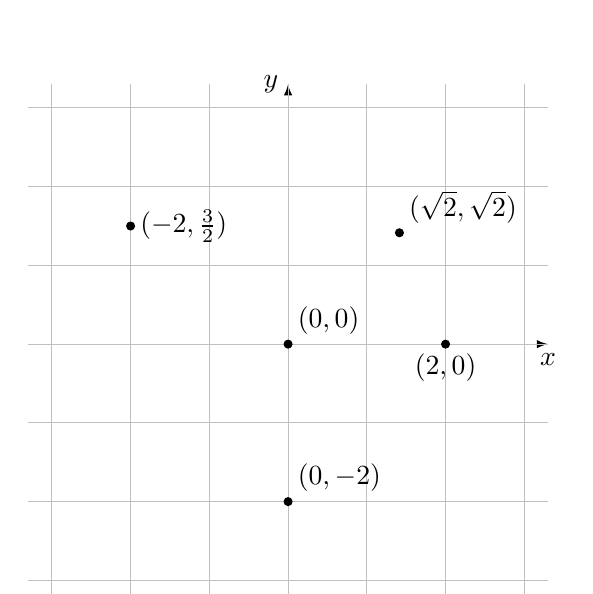
\begin{tikzpicture}
\draw[-latex] (-3.3, 0) -- (3.3, 0) node[below] {$x$} ;
\draw[-latex] (0, -3.3) -- (0, 3.3) node[left] {$y$} ;
\foreach \x in {-3,-2,-1,0,1,2,3} \draw[lightgray] (\x, -3.3) -- (\x, 3.3) ;
\foreach \y in {-3,-2,-1,0,1,2,3} \draw[lightgray] (-3.3, \y) -- (3.3, \y) ;
\draw[fill] (0,0) circle[radius=0.05] node[above right] {$(0,0)$} ;
\draw[fill] ({sqrt(2)},{sqrt(2)}) circle[radius=0.05] node[above right] {$(\sqrt{2},\sqrt{2})$} ;
\draw[fill] (0,-2) circle[radius=0.05] node[above right] {$(0,-2)$} ;
\draw[fill] (2,0) circle[radius=0.05] node[below] {$(2,0)$} ;
\draw[fill] (-2,1.5) circle[radius=0.05] node[right] {$(-2, \frac{3}{2})$} ;
\end{tikzpicture}
\caption{Some points in $\mathbb{R}^2$}
\label{figPointsInR2}
\end{figure}

With this intuition in mind, we set up the following notation.

\begin{notation}
\label{ntnVectorsInRn}
\index{origin}
\index{component}
Let $n \in \mathbb{N}$. Elements of $\mathbb{R}^n$ will be denoted $\vec x, \vec y, \vec z, \dots$\nindex{xvec}{$\vec x$}{vector} \inlatex{vec}\lindexmmc{vec}{$\vec a, \vec b, \dots$} and called ($n$-\textbf{dimensional}) \textbf{vectors}. Given a vector $\vec x \in \mathbb{R}^n$, we write $x_i$ for the $i^{\text{th}}$ \textbf{component} of $\vec x$, so that
\[ \vec x = (x_1,x_2,\dots,x_n) \]
The element $(0,0,\dots,0) \in \mathbb{R}^n$ is called the \textbf{origin} or \textbf{zero vector} of $\mathbb{R}^n$, and is denoted by $\vec 0$.

Moreover, if $\vec x, \vec y \in \mathbb{R}^n$ and $a \in \mathbb{R}$ we write
\[ \vec x + \vec y = (x_1+y_1,x_2+y_2,\dots,x_n+y_n) \quad \text{and} \quad a \vec x = (ax_1,ax_2,\dots,ax_n) \]
\end{notation}

\begin{example}
For all $\vec x \in \mathbb{R}^n$, we have
\[ \vec x + \vec 0 = \vec x \quad \text{and} \quad 1 \vec x = \vec x \]
\end{example}

\begin{definition}
\label{defMagnitude}
\index{magnitude}
\index{distance}
Let $\vec x \in \mathbb{R}^n$. The \textbf{magnitude} of $\vec x$ is the real number $\lVert \vec x \rVert$\nindex{xmag}{$\lVert \vec x \rVert$}{magnitude} \inlatex{lVert\ \textbackslash{}vec\ x\ \textbackslash{}rVert}\lindexmmc{lVert\dots{}\textbackslash{}rVert}{$\lVert \dots{} \rVert$} defined by
\[ \lVert \vec x \rVert = \sqrt{\sum_{i=1}^n x_i^2} = \sqrt{x_1^2+x_2^2+\cdots+x_n^2} \]
Given vectors $\vec x, \vec y \in \mathbb{R}^n$, the \textbf{distance} from $\vec x$ to $\vec y$ is defined to be $\lVert \vec y - \vec x \rVert$. Thus the magnitude of a vector can be thought of as the distance from that vector to the origin.
\end{definition}

\begin{example}
\label{exMagnitudeInR2}
In $\mathbb{R}^2$, \Cref{defMagnitude} says that
\[ \lVert (x,y) \rVert = \sqrt{x^2+y^2} \]
This matches the intuition obtained from the Pythagorean theorem on the sides of right-hand triangles. For example, consider the triangle with vertices $(0,0)$, $(4,0)$ and $(4,3)$:
\begin{center}
\begin{tikzpicture}
\draw (0,0) node [below left] {$(0,0)$}
   -- (4,0) node [below right] {$(4,0)$}
   -- (4,3) node [above right] {$(4,3)$}
   -- (0,0) ;
\end{tikzpicture}
\end{center}
The hypotenuse of the triangle has magnitude
\[ \lVert (4,3) \rVert = \sqrt{4^2+3^2} = \sqrt{25} = 5 \]
\end{example}

\begin{exercise}
\label{exDistanceIsSymmetric}
Let $\vec x, \vec y \in \mathbb{R}^n$. Prove that $\lVert \vec x - \vec y \rVert = \lVert \vec y - \vec x \rVert$. That is, the distance from $\vec x$ to $\vec y$ is equal to the distance from $\vec y$ to $\vec x$.
\end{exercise}

\begin{exercise}
Prove that if $x \in \mathbb{R}$ then the magnitude $\lVert (x) \rVert$ is equal to the absolute value $|x|$.
\end{exercise}

\begin{exercise}
\label{exVectorZeroIffMagnitudeZero}
Let $\vec x \in \mathbb{R}^n$. Prove that $\lVert \vec x \rVert = 0$ if and only if $\vec x = \vec 0$.
\end{exercise}

\subsection*{The triangle inequality and the Cauchy--Schwarz inequality}

The first, and simplest, inequality that we investigate is the (one-dimensional version of the) \textit{triangle inequality} (\Cref{thmTriangleInequality1D}). It is so named because of a generalisation to higher dimensions (\Cref{thmTriangleInequality}), which can be interpreted geometrically as saying that the sum of two side lengths of a triangle is greater than or equal to the third side length.

The triangle inequality is used very frequently in mathematical proofs---you will encounter it repeatedly in this chapter---yet its proof is surprisingly simple.

Before we can prove the triangle inequality, we need the following fact about square roots of real numbers.

\begin{lemma}
\label{lemSquareRootIsOrderPreserving}
Let $x,y \in \mathbb{R}$. If $0 \le x \le y$, then $\sqrt{x} \le \sqrt{y}$.
\end{lemma}
\begin{cproof}
Suppose $0 \le x \le y$. Note that, by definition of the square root symbol, we have $\sqrt{x} \ge 0$ and $\sqrt{y} \ge 0$.

Suppose $\sqrt{x} > \sqrt{y}$. By two applications of \Cref{thmPropertiesOfOrderedFields}(d), we have
\[ y = \sqrt{y} \cdot \sqrt{y} < \sqrt{x} \cdot \sqrt{y} < \sqrt{x} \cdot \sqrt{x} = x \]
so that $y<x$. But this contradicts the assumption that $x \le y$. Hence $\sqrt{x} \le \sqrt{y}$, as required.
\end{cproof}

\begin{theorem}[Triangle inequality in one dimension]
\label{thmTriangleInequality1D}
\index{triangle inequality!in one dimension}
\index{inequality!triangle (one-dimensional)}
Let $x,y \in \mathbb{R}$. Then $|x+y| \le |x|+|y|$. Moreover, $|x+y|=|x|+|y|$ if and only if $x$ and $y$ have the same sign.
\end{theorem}
\begin{cproof}
Note first that $xy \le |xy|$; indeed, $xy$ and $|xy|$ are equal if $xy$ is non-negative, and otherwise we have $xy < 0 < |xy|$. Also $x^2=|x|^2$ and $y^2=|y|^2$. Hence
\[ (x+y)^2 = x^2+2xy+y^2 \le |x|^2+2|xy|+|y|^2 = (|x|+|y|)^2 \]
Taking (nonnegative) square roots yields
\[ |x+y| \le ||x|+|y|| \]
by \Cref{lemSquareRootIsOrderPreserving}. But $|x|+|y| \ge 0$, so $||x|+|y||=|x|+|y|$. This completes the first part of the proof.

Equality holds in the above if and only if $xy=|xy|$, which occurs if and only if $xy \ge 0$. But this is true if and only if $x$ and $y$ are both non-negative or both non-positive---that is, they have the same sign.
\end{cproof}

\begin{example}
Let $x,y \in \mathbb{R}$. We prove that
\[ \frac{|x+y|}{1+|x+y|} \le \frac{|x|}{1+|x|} + \frac{|y|}{1+|y|} \]
First note that, if $0 \le s \le t$, then
\[ \frac{s}{1+s} \le \frac{t}{1+t} \]
To see this, note that
\begin{align*}
s \le t &\Rightarrow 1+s \le 1+t && \text{rearranging} \\
&\Rightarrow \frac{1}{1+t} \le \frac{1}{1+s} && \text{since $1+s,1+t > 0$} \\
&\Rightarrow 1-\frac{1}{1+s} \le 1-\frac{1}{1+t} && \text{rearranging} \\
&\Rightarrow \frac{s}{1+s} \le \frac{t}{1+t} && \text{rearranging}
\end{align*}
Now letting $s=|x+y|$ and $t=|x|+|y|$, we have $s \le t$ by the triangle inequality, and hence
\[ \frac{|x+y|}{1+|x+y|} \le \frac{|x|}{{1+|x|+|y|}} + \frac{|y|}{1+|x|+|y|} \le \frac{|x|}{1+|x|} + \frac{|y|}{1+|y|} \]
as required.
\end{example}

\begin{exercise}
Let $n \in \mathbb{N}$ and let $x_i \in \mathbb{R}$ for each $i \in [n]$. Prove that
\[ \left| \sum_{i=1}^n x_i \right| \le \sum_{i=1}^n |x_i| \]
with equality if and only if the numbers $x_i$ are either all non-positive or all non-negative.
\end{exercise}

\begin{exercise}
Let $x,y \in \mathbb{R}$. Prove that
\[ ||x|-|y|| \le |x-y| \]
\end{exercise}

We will generalise the triangle inequality to arbitrary dimensions in \Cref{thmTriangleInequality}. Our proof will go via the \textit{Cauchy--Schwarz inequality} (\Cref{thmCauchySchwarzInequality}). To motivate the Cauchy--Schwarz inequality, we introduce another geometric notion called the \textit{scalar product} of two vectors.

\begin{definition}
\label{defScalarProduct}
\index{scalar product}
\index{dot product}
Let $\vec x,\vec y \in \mathbb{R}^n$. The \textbf{scalar product} (or \textbf{dot product}) of $\vec x$ with $\vec y$ is the real number $\vec x \cdot \vec y$\nindex{xdoty}{$\vec x \cdot \vec y$}{scalar product} \inlatex{cdot}\lindexmmc{cdot}{$\cdot$} defined by
\[ \vec x \cdot \vec y = \sum_{i=1}^n x_iy_i = x_1y_1+x_2y_2+\cdots+x_ny_n \]
\end{definition}

\begin{example}
\label{exVectorDotItself}
Let $\vec x \in \mathbb{R}^n$. Then $\vec x \cdot \vec x = \lVert \vec x \rVert^2$. Indeed
\[ \vec x \cdot \vec x = \sum_{i=1}^n x_i^2 = \lVert \vec x \rVert^2 \]
\end{example}

\begin{exercise}
\label{exScalarProductIsBilinear}
Let $\vec x, \vec y, \vec z, \vec w \in \mathbb{R}^n$ and let $a,b,c,d \in \mathbb{R}$. Prove that
\[ (a \vec x + b \vec y) \cdot (c \vec z + d \vec w) = ac (\vec x \cdot \vec z) + ad (\vec x \cdot \vec w) + bc( \vec y \cdot \vec z) + bd (\vec y \cdot \vec w) \]
\end{exercise}

Intuitively, the scalar product of two vectors $\vec x$ and $\vec y$ measures the extent to which $\vec x$ and $\vec y$ fail to be \textit{orthogonal}. In fact, if $\theta$ is the acute angle formed between the lines $\ell_1$ and $\ell_2$, where $\ell_1$ passes through $\vec 0$ and $\vec x$ and $\ell_2$ passes through $\vec 0$ and $\vec y$, then a formula for the scalar product of $\vec x$ and $\vec y$ is given by
\[ \vec x \cdot \vec y = \lVert \vec x \rVert \lVert \vec y \rVert \cos \theta \]

\begin{center}
\begin{tikzpicture}[scale=1.5]
\draw [->] (0,0) node [left] {$\vec 0$}
        -- (4,2) node [above right] {$\vec x$} ;
\draw [->] (0,0)
        -- (5,0) node [right] {$\vec y$} ;
\draw [dashed] (4,2) -- (4,0) ;
\draw (3.7,0) -- (3.7,0.3) -- (4,0.3) ;
\draw [<->] (0,-0.3) -- (4,-0.3) ;
\node [below] at (2,-0.3) {$\lVert x \rVert \cos \theta$} ;
\draw [->, domain=0:atan(0.5)] plot ({0.7*cos(\x)},{0.7*sin(\x)}) ;
\node at ({0.85*cos(atan(0.25))}, {0.85*sin(atan(0.25))}) {$\theta$} ;
\end{tikzpicture}
\end{center}

Evidently, $\vec x$ and $\vec y$ are orthogonal if and only if $\cos \theta = 0$, in which case $\vec x \cdot \vec y = 0$ as well. We cannot prove this yet, though, as we have not yet defined trigonometric functions or explored their properties, but hopefully this provides some useful intuition.

The Cauchy--Schwarz inequality provides a useful comparison of the size of a scalar product of two vectors with the magnitudes of the vectors.

\begin{theorem}[Cauchy--Schwarz inequality]
\label{thmCauchySchwarzInequality}
\index{Cauchy--Schwarz inequality}
\index{inequality!Cauchy--Schwarz}
Let $n \in \mathbb{N}$ and let $x_i,y_i \in \mathbb{R}$ for each $i \in [n]$. Then
\[ |\vec x \cdot \vec y| \le \lVert \vec x \rVert \lVert \vec y \rVert \]
with equality if and only if $a\vec x = b\vec y$ for some $a,b \in \mathbb{R}$ which are not both zero.
\end{theorem}
\begin{cproof}
If $\vec y = \vec 0$, then this is trivial: both sides of the equation are equal to zero! So assume that $\vec y \ne \vec 0$. In particular, by \Cref{exVectorZeroIffMagnitudeZero}, we have $\lVert \vec y \rVert > 0$.

Define $k = \dfrac{\vec x \cdot \vec y}{\lVert \vec y \rVert^2}$. Then
\begin{align*}
0 &\le \lVert \vec x - k \vec y \rVert^2 && \text{since squares are nonnegative} \\
&= (\vec x - k \vec y) \cdot (\vec x - k \vec y) && \text{by \Cref{exVectorDotItself}} \\
&= (\vec x \cdot \vec x) - 2k (\vec x \cdot \vec y) + k^2 (\vec y \cdot \vec y) && \text{by \Cref{exScalarProductIsBilinear}} \\
&= \lVert \vec x \rVert^2 - \frac{(\vec x \cdot \vec y)^2}{\lVert y \rVert^2} && \text{by definition of $k$}
\end{align*}
Multiplying through by $\lVert \vec y \rVert^2$, which is non-negative and therefore doesn't change the sign of the inequality, yields
\[ 0 \le \lVert \vec x \rVert^2 \lVert \vec y \rVert^2 - (\vec x \cdot \vec y)^2 \]
which is equivalent to what was to be proved.

Evidently, equality holds if and only if $\lVert \vec x - k \vec y \rVert = 0$, which by \Cref{exVectorZeroIffMagnitudeZero} occurs if and only if $\vec x - k \vec y = 0$. Now:
\begin{itemize}
\item If $\vec x - k\vec y = 0$, then we have
\begin{align*}
&\vec x - k \vec y = 0 && \\
&\Leftrightarrow \vec x - \frac{\vec x \cdot \vec y}{\lVert \vec y \rVert^2} \vec y = 0 && \text{by definition of $k$} \\
&\Leftrightarrow \lVert \vec y \rVert^2 \vec x = (\vec x \cdot \vec y) \vec y && \text{rearranging}
\end{align*}
%% BEGIN EXTRACT (xtrProvingExistsExampleTwo) %%
If $\vec y \ne \vec 0$ then let $a=\lVert \vec y \rVert^2$ and $b=\vec x \cdot \vec y$; otherwise, let $a=0$ and $b=1$. In both cases, we have $a \vec x = b \vec y$ and $a,b$ are not both zero.
%% END EXTRACT %%

If $a \vec x = b \vec y$ for some $a,b \in \mathbb{R}$ not both zero, then either:
\begin{itemize}
\item $a=0$ and $b \ne 0$, in which case $\vec y = 0$ and we have equality in the Cauchy--Schwarz inequality; or
\item $a \ne 0$, in which case $\vec y = \frac{b}{a} \vec x$. Write $c=\frac{b}{a}$. Then
\begin{align*}
|\vec x \cdot \vec y| &= | \vec x \cdot (c \vec x) | && \\
&= |c(\vec x \cdot \vec x)| && \text{by \Cref{exScalarProductIsBilinear}} \\
&= |c| \lVert \vec x \rVert^2 && \text{by \Cref{exVectorDotItself}} \\
&= \lVert \vec x \rVert \lVert c \vec x \rVert && \text{rearranging} \\
&= \lVert \vec x \rVert \lVert \vec y \rVert &&
\end{align*}
\end{itemize}
In either case, we have equality in the Cauchy--Schwarz inequality.
\end{itemize}

So equality holds if and only if $a \vec x = b \vec y$ for some $a,b \in \mathbb{R}$ not both zero.
\end{cproof}

\begin{example}
Let $a,b,c \in \mathbb{R}$. We'll prove that
\[ ab+bc+ca \le a^2+b^2+c^2 \]
and examine when equality holds.

Letting $\vec x = (a,b,c)$ and $\vec y = (b,c,a)$ yields
\[ \vec x \cdot \vec y = ab+bc+ca \]
and
\[ \lVert \vec x \rVert = \sqrt{a^2+b^2+c^2} = \sqrt{b^2+c^2+a^2} = \lVert \vec y \rVert \]
Hence $\lVert \vec x \rVert \lVert \vec y \rVert = a^2+b^2+c^2$. By the Cauchy--Schwarz inequality, it follows that
\[ \vec x \cdot \vec y = ab+bc+ca \le a^2+b^2+c^2 = \lVert \vec x \rVert \lVert \vec y \rVert \]
as required. Equality holds if and only if $k(a,b,c) = \ell(b,c,a)$ for some $k,\ell \in \mathbb{R}$ not both zero. We may assume $k \ne 0$---otherwise, swap the vectors $\vec x$ and $\vec y$ in what follows. Then, letting $t=\frac{\ell}{k}$, we have
\begin{align*}
&k(a,b,c) = \ell(b,c,a) && \\
&\Leftrightarrow (a,b,c) = (tb,tc,ta) && \text{by definition of $t$} \\
&\Leftrightarrow (a,b,c) = (t^2c,t^2a,t^2b) && \text{substituting $a=tb$ etc.} \\
&\Leftrightarrow (a,b,c) = (t^3a,t^3b,t^3c) && \text{substituting $a=tb$ etc.\ again} \\
&\Leftrightarrow \vec x = t^3 \vec x
\end{align*}
This occurs if and only if either $(a,b,c)=(0,0,0)$, or $t=1$, in which case
\[ (a,b,c) = (tb,tc,ta) = (b,c,a) \]
So equality holds if and only if $a=b=c$.
\end{example}

\begin{exercise}
Let $r \in \mathbb{N}$ and let $a_1,a_2,\dots,a_r \in \mathbb{R}$ be such that $a_1^2+a_2^2+\cdots+a_n^2=6$. Prove that
\[ (a_1+2a_2+\cdots+na_n)^2 \le n(n+1)(2n+1) \]
and determine when equality holds.
\end{exercise}

We now use the Cauchy--Schwarz inequality to generalise the one-dimensional version of the triangle inequality (\Cref{thmTriangleInequality1D}) to arbitrary (finite) dimensions.

\begin{theorem}[Triangle inequality]
\label{thmTriangleInequality}
\index{triangle inequality}
\index{inequality!triangle}
Let $\vec x, \vec y \in \mathbb{R}^n$. Then
\[ \lVert \vec x + \vec y \rVert \le \lVert \vec x \rVert + \lVert \vec y \rVert \]
with equality if and only if $a\vec x = b\vec y$ for some real numbers $a,b \ge 0$.
\end{theorem}

\begin{cproof}
We proceed by calculation:
\begin{align*}
\lVert \vec x + \vec y \rVert^2
&= (\vec x + \vec y) \cdot (\vec x + \vec y) && \text{by \Cref{exVectorDotItself}} \\
&= (\vec x \cdot \vec x) + 2(\vec x \cdot \vec y) + (\vec y \cdot \vec y) && \text{by \Cref{exScalarProductIsBilinear}} \\
&\le (\vec x \cdot \vec x) + 2|\vec x \cdot \vec y| + (\vec y \cdot \vec y) && \text{since $a \le |a|$ for all $a \in \mathbb{R}$} \\
&\le \lVert \vec x \rVert^2 + 2\lVert x \rVert \lVert y \rVert + \lVert \vec y \rVert^2 && \text{by \Cref{exVectorDotItself} and Cauchy--Schwarz} \\
&= (\lVert \vec x \rVert + \lVert \vec y \rVert)^2 && \text{rearranging}
\end{align*}

Taking (nonnegative) square roots of both sides yields
\[ \lVert \vec x + \vec y \rVert \le \lVert \vec x \rVert + \lVert \vec y \rVert \]
by \Cref{lemSquareRootIsOrderPreserving}, as required.

Equality holds if and only if the two `$\le$' symbols in the above derivation are in fact `$=$' symbols.
\begin{itemize}
\item The first inequality is equality if and only if $\vec x \cdot \vec y = |\vec x \cdot \vec y|$, which holds if and only if $\vec x \cdot \vec y \ge 0$.
\item The second inequality is equality if and only if equality holds in the Cauchy--Schwarz inequality. In turn, this occurs if and only if $a\vec x = b \vec y$ for some $a,b \in \mathbb{R}$. We may, moreover, assume that $a \ge 0$---if not, replace $a$ and $b$ by their negatives.
\end{itemize}
If $a=0$ then we can take $b=0$.
%% BEGIN EXTRACT {xtrSoExampleTwo} %%
If $a>0$, then by \Cref{exVectorDotItself} and \Cref{exScalarProductIsBilinear}, we have
\[ \vec x \cdot \left( \frac{b}{a} \vec x \right) = \frac{b}{a} \lVert \vec x \rVert^2 \]
which is non-negative if and only if $b \ge 0$, since we are assuming that $a \ge 0$.
%% END EXTRACT %%

Thus, equality holds in the triangle inequality if and only if $a\vec x = b\vec y$ for some $a,b \ge 0$.
\end{cproof}

This general version of the triangle inequality has a geometric interpretation in terms of---you guessed it---triangles. Any three points $\vec a, \vec b, \vec c \in \mathbb{R}^n$ form a (potentially flat) triangle:

\begin{center}
\begin{tikzpicture}
\draw (0,2) -- (7,0) node[pos=0, left] {$\vec a$}
                     node[midway, below left] {$u$}
            -- (3,4) node[pos=0, right] {$\vec b$}
                     node[midway, above right] {$v$}
            -- (0,2) node[pos=0, above] {$\vec c$}
                     node[midway, above left] {$w$};
\end{tikzpicture}
\end{center}

The side lengths $u,v,w$ are given by the following equations:
\[ u = \lVert \vec b - \vec a \rVert, \quad v = \lVert \vec c - \vec b \rVert, \quad w = \lVert \vec a - \vec c \rVert \]
The triangle inequality says tells us that $u \le v + w$. Indeed:
\begin{align*}
u &= \lVert \vec b - \vec a \rVert && \text{by definition of $u$} \\
&= \lVert (\vec b - \vec c) + (\vec c - \vec a) \rVert && \text{rearranging} \\
&\le \lVert \vec b - \vec c \rVert + \lVert \vec c - \vec a \rVert && \text{by the triangle inequality} \\
&= \lVert \vec c - \vec b \rVert + \lVert \vec a - \vec c \rVert && \text{by \Cref{exDistanceIsSymmetric}} \\
&= v + w && \text{by definition of $v$ and $w$}
\end{align*}

That is, the triangle inequality says that the sum of two side lengths of a triangle is greater than or equal to the third side length. Moreover, it tells us $u=v+w$ precisely when $k(\vec a - \vec c) = \ell(\vec c - \vec b)$ for some $k,\ell \ge 0$. If $k=0$ then
\[ \vec c \quad = \quad \vec b \quad = \quad 0 \vec a + (1-0) \vec b \]
if $k>0$, then $k+\ell>0$, so we have
\[ \vec c \quad = \quad \frac{k}{k+\ell} \vec a + \frac{\ell}{k+\ell} \vec b \quad = \quad \frac{k}{k+\ell} \vec a + \left( 1 - \frac{k}{k+\ell} \right)\vec b \]
Examining this a bit more closely yields that $u=v+w$ if and only if
\[ \vec c = t\vec a + (1-t) \vec b \]
for some $0 \le t \le 1$, which is to say precisely that $\vec c$ lies on the line segment between $\vec a$ and $\vec b$. In other words, equality holds in the triangle inequality only if the three vertices of the triangle are \textit{collinear}, which is to say that the triangle whose vertices are the points $\vec a$, $\vec b$ and $\vec c$, is flat.

\subsection*{Inequalities of means}

Our goal now is to explore different kinds of average---specifically, \textit{means}---of finite sets of non-negative real numbers. We will compare the relative sizes of these means with respect to one-another, with emphasis on three particular kinds of mean: the \textit{arithmetic mean} (\Cref{defArithmeticMean}), the \textit{geometric mean} (\Cref{defGeometricMean}) and the \textit{harmonic mean} (\Cref{defHarmonicMean}). These means in fact assemble into a continuum of means, called \textit{generalised means} (\Cref{defGeneralisedMean}), all of which can be compared with one another.

\begin{definition}
\label{defArithmeticMean}
\index{mean!arithmetic}
Let $n \ge 1$. The (\textbf{arithmetic}) \textbf{mean} of real numbers $x_1,\dots,x_n$ is
\[ \frac{1}{n} \sum_{i=1}^n x_i = \frac{x_1 + x_2 + \cdots + x_n}{n} \]
\end{definition}

\begin{definition}
\label{defGeometricMean}
\index{mean!geometric}
Let $n \ge 1$. The \textbf{geometric mean} of non-negative real numbers $x_1,\dots,x_n$ is
\[ \sqrt[n]{\prod_{i=1}^n x_i} = \sqrt[n]{x_1 \cdot x_2 \cdot \dots \cdot x_n} \]
\end{definition}

The following theorem is commonly known as the \textbf{AM--GM inequality}.

\begin{theorem}[Inequality of arithmetic and geometric means]
\label{thmAMGMInequality}
\index{AM--GM inequality}
\index{inequality!of arithmetic and harmonic means}
Let $n \in \mathbb{N}$ and $x_1,x_2,\dots,x_n \ge 0$. Then
\[ \underbrace{\sqrt[n]{x_1 \cdots x_n}}_{\text{geometric mean}} \le \underbrace{\frac{x_1 + \cdots + x_n}{n}}_{\text{arithmetic mean}} \]
with equality if and only if $x_1 = \cdots = x_n$.
\end{theorem}
\begin{cproof}[when $n=2$]
We need to show that, if $x,y \in \mathbb{R}$ with $x, y \ge 0$, then
\[ \sqrt{xy} \le \frac{x+y}{2} \]
with equality if and only if $x=y$.

First note that the square roots of $x$ and $y$ exist since they are non-negative. Now
\begin{align*}
0 &\le (\sqrt{x}-\sqrt{y})^2 && \text{since squares are nonnegative} \\
&= (\sqrt{x})^2 - 2\sqrt{x}\sqrt{y} + (\sqrt{y})^2 && \text{expanding} \\
&= x - 2\sqrt{xy} + y && \text{rearranging}
\end{align*}

Rearranging the inequality $0 \le x-2\sqrt{xy}+y$ yields the desired result.

If $\sqrt{xy} = \frac{x+y}{2}$, then we can rearrange the equation as follows:
\begin{align*}
\sqrt{xy} = \frac{x+y}{2} &\Rightarrow 2\sqrt{xy} = x+y && \text{multiplying by $2$} \\
&\Rightarrow 4xy = x^2+2xy+y^2 && \text{squaring both sides} \\
&\Rightarrow x^2-2xy+y^2 = 0 && \text{rearranging} \\
&\Rightarrow (x-y)^2 = 0 && \text{factorising} \\
&\Rightarrow x-y = 0 && \text{since $a^2=0 \Rightarrow a=0$ for $a \in \mathbb{R}$} \\
&\Rightarrow x=y && \text{rearranging}
\end{align*}
So we have proved both parts of the theorem.
\end{cproof}

\begin{example}
We use the AM--GM inequality to prove that the area of a rectangle with fixed perimeter is maximised when the rectangle is a square.

Indeed, fix a perimeter $p > 0$, and let $x,y > 0$ be side lengths of a rectangle with perimeter $p$---that is, $x$ and $y$ satisfy the equation $2x+2y=p$. The area $a$ of the rectangle satisfies $a=xy$. By the AM--GM inequality, we have
\[ a = xy \le \left( \frac{x+y}{2} \right)^2 = \frac{p^2}{16} \]
Equality holds if and only if $x=y$, in other words, if and only if the rectangle is a square.
\end{example}

\begin{exercise}
Let $a,b > 0$ be real numbers. Prove that $\displaystyle \frac{a^2+b^2}{2} \ge ab$.
\end{exercise}

\begin{example}
Let $x>0$. We find the minimum possible value of $x+\frac{9}{x}$. By the AM--GM inequality, we have
\[ x+\frac{9}{x} \ge 2\sqrt{x \cdot \frac{9}{x}} = 2 \sqrt{9} = 6 \]
with equality if and only if $x=\frac{9}{x}$, which occurs if and only if $x=3$. Hence the minimum value of $x+\frac{9}{x}$ when $x>0$ is $6$.
\end{example}

\begin{exercise}
Let $x>0$ and let $n \in \mathbb{N}$. Find the minimum possible value of $\displaystyle \sum_{k=-n}^n x^k$.
\end{exercise}

\Cref{exAMGMForPowersOf2,exAMGMForPredecessors} complete the proof of the AM--GM inequality (\Cref{thmAMGMInequality}). Before proceeding with the exercises, let's fix some notation: for each $n \in \mathbb{N}$, let $p_{\text{AM--GM}}(n)$ be the assertion that
the AM--GM inequality holds for collections of $n$ numbers; that is, $p_{\text{AM--GM}}(n)$ is the assertion:
\begin{quote}
For all $x_1,x_2,\dots,x_n \ge 0$, we have
\[ \sqrt[n]{\prod_{i=1}^n x_i} \le \frac{1}{n} \sum_{i=1}^n x_i \]
with equality if and only if $x_1=x_2=\cdots=x_n$.
\end{quote}
Note that we already proved $p_{\text{AM--GM}}(2)$.

\begin{exercise}
\label{exAMGMForPowersOf2}
Let $r \in \mathbb{N}$ and let $x_1,x_2,\dots,x_{2r} \in \mathbb{R}$. Write
\[ a = \frac{1}{r} \sum_{i=1}^r x_i \quad \text{and} \quad g = \sqrt[r]{\prod_{i=1}^r x_i} \]
for the arithmetic and geometric means, respectively, of the numbers $x_1,\dots,x_r$; write
\[ a' = \frac{1}{r} \sum_{i=r+1}^{2r} x_i \quad \text{and} \quad g' = \sqrt[r]{\prod_{i=r+1}^{2r} x_i} \]
for the arithmetic and geometric means, respectively, of the numbers $x_{r+1},\dots,x_{2r}$; and write
\[ A = \frac{1}{2r} \sum_{i=1}^{2r} x_i \quad \text{and} \quad G = \sqrt[2r]{\prod_{i=1}^{2r} x_i} \]
for the arithmetic and geometric means, respectively, of all the numbers $x_1,\dots,x_{2r}$.

Prove that
\[ A = \frac{a+a'}{2} \quad \text{and} \quad G=\sqrt{gg'} \]
Deduce that, for each $r \in \mathbb{N}$, if $p_{\text{AM--GM}}(r)$ is true then $p_{\text{AM--GM}}(2r)$ is true. Deduce further than $p_{\text{AM--GM}}(2^m)$ is true for all $m \in \mathbb{N}$.
\end{exercise}

\begin{exercise}
\label{exAMGMForPredecessors}
Let $r \ge 2$ and let $x_1,\dots,x_{r-1} \in \mathbb{N}$. Define
\[ x_r = \frac{1}{r-1} \sum_{i=1}^{r-1} x_i \]
Prove that
\[ \frac{1}{r}\sum_{i=1}^r x_i = x_r \]
Assuming $p_{\text{AM--GM}}(r)$, deduce that
\[ x_r^r \ge \prod_{i=1}^r x_i = \left(\prod_{i=1}^{r-1} x_i\right) \cdot x_r \]
with equality if and only if $x_1=x_2=\cdots=x_r$. Deduce that $p_{\text{AM--GM}}(r)$ implies $p_{\text{AM--GM}}(r-1)$. Use \Cref{exAMGMForPowersOf2} to deduce further that $p_{\text{AM--GM}}(n)$ is true for all $n \ge 1$.
\end{exercise}

We now introduce another kind of mean, called the \textit{harmonic mean}.

\begin{definition}
\label{defHarmonicMean}
\index{mean!harmonic}
Let $n \in \mathbb{N}$. The \textbf{harmonic mean} of nonzero real numbers $x_1,x_2,\dots,x_n$ is
\[ \left( \frac{1}{n} \sum_{i=1}^n x_i^{-1} \right)^{-1} = \cfrac{n}{\frac{1}{x_1} + \frac{1}{x_2} + \cdots + \frac{1}{x_n}} \]
\end{definition}

The harmonic mean of two nonzero real numbers $x$ and $y$ has a simpler expression:
\[ \left( \frac{x^{-1}+y^{-1}}{2} \right)^{-1} = \frac{2xy}{x+y} \]

The harmonic mean arises naturally when considering rates of change of quantities over fixed amounts of time.

\begin{example}
The cities of York and Leeds are located $d>0$ miles apart. Two cars drive from York to Leeds, then immediately turn around and drive back. The two cars depart from York at the same time and arrive back in York at the same time.
\begin{itemize}
\item The first car drives from York to Leeds at a constant speed of $u$ miles per hour, and drives back to York at a constant speed of $v$ miles per hour.
\item The second car drives from York to Leeds and back again at the same constant speed of $w$ miles per hour.
\end{itemize}
According to the following formula from physics:
\[ \text{speed} \times \text{time} = \text{distance} \]
the time spent driving by the first car is $\frac{d}{u} + \frac{d}{v}$, and the time spent driving by the second car is $\frac{2d}{w}$.

Since the cars spend the same amount of time driving, it follows that
\[ \frac{2d}{w} = \frac{d}{u} + \frac{d}{v} \qquad \Rightarrow \qquad w = \frac{2uv}{u+v} \]
That is, the second car's speed is the harmonic mean of the two speeds driven by the first car.
\end{example}

As might be expected, we now prove a theorem relating the harmonic means with the other means we have established so far---this theorem is known as the \textbf{GM--HM inequality}.

\begin{theorem}[Inequality of geometric and harmonic means]
\label{thmGMHMInequality}
\index{GM--HM inequality}
\index{inequality!of geometric and harmonic means}
Let $n \in \mathbb{N}$ and $x_1,x_2,\dots,x_n > 0$. Then
\[ \underbrace{\cfrac{n}{\frac{1}{x_1} + \frac{1}{x_2} + \cdots + \frac{1}{x_n}}}_{\text{harmonic mean}} \le \underbrace{\sqrt[n]{x_1x_2 \cdots x_n}}_{\text{geometric mean}} \]
with equality if and only if $x_1 = \cdots = x_n$.
\end{theorem}
\begin{cproof}[when $n=2$]
We need to prove that if $x,y > 0$, then
\[ \frac{2}{\frac{1}{x} + \frac{1}{y}} \le \sqrt{xy} \]
This is almost immediate from the AM--GM inequality (\Cref{thmAMGMInequality}). Indeed, since all numbers in sight are positive, we can take reciprocals to see that this inequality is equivalent to the assertion that
\[ \frac{1}{\sqrt{xy}} \le \frac{x^{-1} + y^{-1}}{2} \]
But $\frac{1}{\sqrt{xy}} = \sqrt{x^{-1}y^{-1}}$, so this is immediate from the AM--GM inequality.
\end{cproof}

\begin{exercise}
Prove the GM--HM inequality for general values of $n \in \mathbb{N}$.
\end{exercise}

Another example of a mean that has applications in probability theory and statistics is that of the \textit{quadratic mean}.

\begin{definition}
\label{defQuadraticMean}
\index{mean!quadratic}
\index{root-mean-square}
Let $n \in \mathbb{N}$. The \textbf{quadratic mean} (or \textbf{root-mean-square}) of real numbers $x_1,x_2,\dots,x_n$ is
\[ \left( \frac{1}{n} \sum_{i=1}^n x_i^2 \right)^{\frac{1}{2}} = \sqrt{\frac{x_1^2+x_2^2+\cdots+x_n^2}{n}} \]
\end{definition}

The following theorem is, predictably, known as the \textbf{QM--AM inequality} (or \textbf{RMS--AM inequality}); it is a nice application of the Cauchy--Schwarz inequality.

\begin{theorem}[Inequality of quadratic and arithmetic means]
\label{thmQMAMInequality}
\index{QM--AM inequality}
\index{inequality!of quadratic and arithmetic means}
Let $n > 0$ and $x_1,x_2,\dots,x_n \ge 0$. Then
\[ \underbrace{\frac{x_1 + \cdots + x_n}{n}}_{\text{arithmetic mean}} \le \underbrace{\sqrt{\frac{x_1^2+x_2^2+\cdots+x_n^2}{n}}}_{\text{quadratic mean}} \]
with equality if and only if $x_1 = \cdots = x_n$.
\end{theorem}

\begin{cproof}
Define
\[ \vec x = (x_1,x_2,\dots,x_n) \quad \text{and} \quad \vec y = (1,1,\dots,1) \]
Then
\begin{align*}
x_1+x_2+\cdots+x_n
&= \vec x \cdot \vec y && \text{by definition of scalar product} \\
&\le \lVert \vec x \rVert \lVert \vec y \rVert && \text{by Cauchy--Schwarz} \\
&= \sqrt{x_1^2+x_2^2+\cdots+x_n^2} \cdot \sqrt{n} && \text{evaluating the magnitudes}
\end{align*}
Dividing through by $n$ yields
\[ \frac{x_1+x_2+\cdots+x_n}{n} \le \sqrt{\frac{x_1^2+x_2^2+\cdots+x_n^2}{n}} \]
as required. Equality holds if and only if equality holds in the Cauchy--Schwarz inequality, which occurs if and only if
\[ (ax_1,ax_2,\dots,ax_n)=(b,b,\dots,b) \]
for some $a,b \in \mathbb{R}$ not both zero. If $a=0$ then $b=0$, so we must have $a \ne 0$. Hence equality holds if and only if $x_i=\frac{b}{a}$ for all $i \in [n]$---in particular, if and only if $x_1=x_2=\cdots=x_n$.
\end{cproof}

To summarise, what we have proved so far is
\[ \begin{matrix} \text{harmonic} \\ \text{mean} \end{matrix} \quad \overset{(\ref{thmGMHMInequality})}{\le} \quad \begin{matrix} \text{geometric} \\ \text{mean} \end{matrix} \quad \overset{(\ref{thmAMGMInequality})}{\le} \quad \begin{matrix} \text{arithmetic} \\ \text{mean} \end{matrix} \quad \overset{(\ref{thmQMAMInequality})}{\le} \quad \begin{matrix} \text{quadratic} \\ \text{mean} \end{matrix} \]
with equality in each case if and only if the real numbers whose means we are taking are all equal.

The following exercise allows us to bookend our chain of inequalities with the minimum and maximum of the collections of numbers.

\begin{exercise}
\label{exMinMeanMaxInequalities}
Let $n > 0$ and let $x_1,x_2,\dots,x_n$ be positive real numbers. Prove that
\[ \mathrm{min} \{ x_1,x_2,\dots,x_n \} \le \left( \frac{1}{n} \sum_{i=1}^n x_i^{-1} \right)^{-1} \quad \text{and} \quad \mathrm{max} \{ x_1,x_2,\dots,x_n \} \ge \left( \frac{1}{n} \sum_{i=1}^n x_i^2 \right)^{\frac{1}{2}} \]
with equality in each case if and only if $x_1=x_2=\cdots=x_n$.
\end{exercise}

\subsection*{\optmark{Generalised means}}

We conclude this section by mentioning a generalisation of the results we have proved about means. We are not yet ready to prove the results that we mention; they are only here for the sake of interest.

\begin{definition}
\label{defExtendedRealLine}
\index{extended real number line}
The \textbf{extended real number line} is the (ordered) set $[-\infty, \infty]$, defined by
\[ [-\infty,\infty] = \mathbb{R} \cup \{ -\infty, \infty \} \]
where $\mathbb{R}$ is the set of real numbers with its usual ordering, and $-\infty,\infty$ are new elements ordered in such a way that $-\infty < x < \infty$ for all $x \in \mathbb{R}$.
\end{definition}

Note that the extended real line does \textit{not} form a field---the arithmetic operations are not defined on $-\infty$ or $\infty$, and we will at no point treat $-\infty$ and $\infty$ as real numbers; they are merely elements which extend the reals to add a least element and a greatest element.

\begin{definition}
\label{defGeneralisedMean}
\index{mean!generalised}
Let $p \in [-\infty,\infty]$, let $n \in \mathbb{N}$, and let $x_1,x_2,\dots,x_n$ be positive real numbers. The \textbf{generalised mean with exponent $p$} (or simply $p$-\textbf{mean}) $x_1,x_2,\dots,x_n$ is the real number $M_p(x_1,x_2,\dots,x_n)$ defined by
\[ M_p(x_1,x_2,\dots,x_n) = \left( \frac{1}{n} \sum_{i=1}^n x_i^p \right)^{\frac{1}{p}} \]
if $p \not \in \{ -\infty, 0, \infty \}$, and by
\[ M_p(x_1,x_2,\dots,x_n) = \lim_{q \to p} M_q(x_1,x_2,\dots,x_n) \]
if $p \in \{ -\infty, 0, \infty \}$, where the notation $\lim\limits_{q \to p}$ refers to the \textit{limit} as $q$ tends to $p$, as discussed in \Cref{secLimitsOfFunctions}.
\end{definition}

We can see immediately that the harmonic, arithmetic and quadratic means of a finite set of positive real numbers are the $p$-means for a suitable value of $p$: the harmonic mean is the $(-1)$-mean, the arithmetic mean is the $1$-mean, and the quadratic mean is the $2$-mean. Furthermore, \Cref{propZeroAndInfinityMeans} exhibits the \textit{minimum} as the $(-\infty)$-mean, the \textit{geometric mean} as the $0$-mean, and the \textit{maximum} as the $\infty$-mean.

\begin{proposition}
\label{propZeroAndInfinityMeans}
Let $n > 0$ and let $x_1,x_2,\dots,x_n \ge 0$. Then
\begin{itemize}
\item $M_{-\infty}(x_1,x_2,\dots,x_n) = \mathrm{min}\{ x_1,x_2,\dots,x_n \}$;
\item $M_0(x_1,x_2,\dots,x_n) = \sqrt[n]{x_1x_2\cdots x_n}$; and
\item $M_{\infty}(x_1,x_2,\dots,x_n) = \mathrm{max}\{ x_1,x_2,\dots,x_n \}$. \qed
\end{itemize}
\end{proposition}

All of the inequalities of means we have seen so far will be subsumed by \Cref{thmGeneralisedMeanInequality}, which compares the $p$-mean and $q$-mean of a set of numbers for all values of $p,q \in [-\infty,\infty]$.

\begin{theorem}
\label{thmGeneralisedMeanInequality}
\index{inequality!of generalised means}
Let $n > 0$, let $x_1,x_2,\dots,x_n \ge 0$ and let $p,q \in [-\infty,\infty]$ with $p<q$. Then
\[ M_p(x_1,x_2,\dots,x_n) \le M_q(x_1,x_2,\dots,x_n) \]
with equality if and only if $x_1=x_2=\cdots=x_n$. \qed
\end{theorem}

\Cref{thmGeneralisedMeanInequality} implies each of the following:
\begin{itemize}
\item \textbf{HM--min inequality} (\Cref{exMinMeanMaxInequalities}): take $p=-\infty$ and $q=-1$;
\item \textbf{GM--HM inequality} (\Cref{thmGMHMInequality}): take $p=-1$ and $q=0$;
\item \textbf{AM--GM inequality} (\Cref{thmAMGMInequality}): take $p=0$ and $q=1$;
\item \textbf{QM--AM inequality} (\Cref{thmQMAMInequality}): take $p=1$ and $q=2$;
\item \textbf{max--QM inequality} (\Cref{exMinMeanMaxInequalities}): take $p=2$ and $q=\infty$.
\end{itemize}

\newpage
% !TeX root = ../../infdesc.tex
\section{Completeness and convergence}
\secbegin{secCompletenessConvergence}

For most of the results that we proved in \Cref{secInequalitiesMeans}, it did not matter that we were talking about real numbers. We could just as well have been working with any other ordered field, such as the rational numbers---that is, most of the results in \Cref{secInequalitiesMeans} remain true by replacing $\mathbb{R}$ by $\mathbb{Q}$ (or any other ordered field) throughout.

From here onwards, we isolate the property of $\mathbb{R}$ that separates it from $\mathbb{Q}$---namely, \textit{completeness}. It is completeness that will allow us to define and explore the fundamental concepts of mathematical analysis: sequences, functions, convergence, limits, continuity, differentiability, and so on.

The property of completeness concerns least upper bounds for certain sets of real numbers.

\begin{definition}
\label{defSupremumOfSubsetOfR}
\index{upper bound!of subset of $\mathbb{R}$}
\index{supremum!of subset of $\mathbb{R}$}
Let $A \subseteq \mathbb{R}$. A real number $m$ is an \textbf{upper bound} for $A$ if $a \le m$ for all $a \in A$. A \textbf{supremum} of $A$ is a \textit{least} upper bound of $A$; that is, a real number $m$ such that:
\begin{enumerate}[(i)]
\item $m$ is an upper bound of $A$---that is, $a \le m$ for all $a \in A$; and
\item $m$ is least amongst all upper bounds for $A$---that is, for all $x \in \mathbb{R}$, if $a \le x$ for all $a \in A$, then $x \le m$.
\end{enumerate}
\end{definition}

\begin{example}
We prove that $1$ is a supremum of the open interval $(0,1)$.
\begin{enumerate}[(i)]
\item Let $a \in (0,1)$. Then $a < 1$, so that $1$ is an upper bound of $(0,1)$.
\item Let $x \in \mathbb{R}$ be another upper bound of $(0,1)$. If $x < 1$, then we have
\[ x = \dfrac{x+x}{2} < \dfrac{x+1}{2} < \dfrac{1+1}{2} = 1 \]
and so $x < \dfrac{x+1}{2} \in (0,1)$. This contradicts the assumption that $x$ is an upper bound of $(0,1)$. It follows that $x \ge 1$, as required.
\end{enumerate}
Hence $1$ is indeed a supremum of $(0,1)$.
\end{example}

\begin{exercise}
\label{exDefineLowerBoundInfimum}
\index{lower bound!of subset of $\mathbb{R}$}
\index{infimum!of subset of $\mathbb{R}$}
Define the notions of \textbf{lower bound} and \textbf{infimum}, and find the infimum of the open interval $(0,1)$.
\end{exercise}

The following proposition provides a convenient way of testing whether a real number is a supremum of a subset.

\begin{proposition}
\label{propSupremumEpsilon}
Let $A \subseteq \mathbb{R}$ and suppose $m \in \mathbb{R}$ is an upper bound of $A$. Then $m$ is a supremum of $A$ if and only if, for all $\varepsilon > 0$, there exists $a \in A$ such that $a > m-\varepsilon$.
\end{proposition}

\begin{cproof}
\fixlistskip
\begin{itemize}
\item ($\Rightarrow$). Suppose $m$ is a supremum of $A$, and let $\varepsilon > 0$. If there is no $a \in A$ such that $a > m - \varepsilon$, then $a \le m-\varepsilon$ for all $a \in A$. But this contradicts the assumption that $m$ is a supremum of $a$, since $m-\varepsilon$ is an upper bound of $A$ that is less than $m$. So there exists $a \in A$ with $a > m - \varepsilon$, as required.

\item ($\Leftarrow$). Suppose that, for all $\varepsilon > 0$, there exists $a \in A$ with $a > m-\varepsilon$, and let $x \in \mathbb{R}$ be an upper bound of $A$. In order to prove that $m$ is a supremum of $A$, we must prove that $m \le x$.

Suppose $x < m$, and define $\varepsilon = m-x$. Then $\varepsilon > 0$, so there exists $a \in A$ such that
\[ a > m - \varepsilon = m - (m-x) = x \]
But this contradicts the assumption that $x$ is an upper bound of $A$. So we must have $m \le x$, as required.
\end{itemize}
\end{cproof}

\begin{theorem}[Uniqueness of suprema]
Let $A$ be a subset of $\mathbb{R}$. If $m_1$ and $m_2$ are suprema of $A$, then $m_1 = m_2$.
\end{theorem}

\begin{cproof}
Since $m_1$ is an upper bound of $A$ and $m_2$ is a supremum of $A$, we have $m_2 \le m_1$ by \Cref{defSupremumOfSubsetOfR}(ii). Likewise, since $m_2$ is an upper bound of $A$ and $m_1$ is a supremum of $A$, we have $m_1 \le m_2$ by \Cref{defSupremumOfSubsetOfR}(ii) again. But this implies that $m_1 = m_2$.
\end{cproof}

An analogous result proves that a subset of $\mathbb{R}$ may have at most one infimum. This allows us to introduce the following notation.

\begin{definition}
\nindex{supremum}{$\mathrm{sup}(A)$}{supremum}
\nindex{infimum}{$\mathrm{inf}(A)$}{infimum}
Let $A \subseteq \mathbb{R}$. The supremum of $A$, if it exists is denoted by $\mathrm{sup}(A)$ \inlatex{mathrm\{sup\}}\lindexmmc{mathrm}{$\mathrm{Aa}, \mathrm{Bb}, \dots$}; the infimum of $A$, if it exists, is denoted by $\mathrm{inf}(A)$ \inlatex{mathrm\{inf\}}.
\end{definition}

Now that we are more familiar with suprema, here is the completeness axiom in its full glory.

\begin{axiom}[Completeness axiom]
\label{axCompletenessOfR}
Let $A \subseteq \mathbb{R}$ be inhabited. If $A$ has an upper bound, then $A$ has a supremum.
\end{axiom}

The true power of the completeness axiom will become apparent later in the section when we discuss the existence of limits of sequences of real numbers.

Before we embark on that adventure, we first prove that the rational numbers are \textit{not} complete, by exhibiting a subset of $\mathbb{Q}$ that has no rational supremum.

\begin{proposition}
\label{propIrrationalsNotComplete}
Let $A = \{ x \in \mathbb{Q} \mid x^2 < 2 \}$. Then $A$ does not have a rational supremum.
\end{proposition}

A quick proof of \Cref{propIrrationalsNotComplete} would be to verify that $\sqrt{2}$, which is irrational, is a supremum of $A$, and use uniqueness of suprema to deduce that there can be no rational supremum. However, this is cheating. Failure of completeness is an \textit{intrinsic} property---we should be able to prove \Cref{propIrrationalsNotComplete} without venturing outside of the realm of rational numbers at all. That is, we cannot use irrational numbers in our proof. This makes the proof significantly longer, but significantly more satisfying.

\begin{cproof}[of \Cref{propIrrationalsNotComplete}]
Towards a contradiction, suppose that $A$ has a supremum $q$.

First note that $q>0$. Indeed, $1^2 < 2$, so that $1 \in A$, and so $q \ge 1 > 0$.

Next, we prove that $q^2 = 2$. Indeed:
\begin{itemize}
\item Assume $q^2 < 2$, so that $2-q^2 > 0$. For each $n \ge 1$, we have
\[ \left( q + \frac{1}{n} \right)^2 ~=~ q^2 + \frac{2q}{n} + \frac{1}{n^2} \]
Choose $n$ sufficiently large that $\dfrac{2q}{n} < \dfrac{2-q^2}{2}$ and $\dfrac{1}{n^2} < \dfrac{2-q^2}{2}$. Then by the above, we observe that
\[ \left( q + \frac{1}{n} \right)^2 ~<~ q^2 + \dfrac{2-q^2}{2} + \dfrac{2-q^2}{2} ~=~ q^2 + (2-q^2) ~=~ 2 \]
and so $q+\frac{1}{n} \in A$. But $q + \frac{1}{n} > q$, so this contradicts the assumption that $q$ is an upper bound of $A$.

\item Assume $q^2 > 2$, so that $q^2-2 > 0$. For each $n \ge 1$, we have
\[ \left( q - \frac{1}{n} \right)^2 = q^2 - \frac{1}{n} \left( 2q - \frac{1}{n} \right) \]

Choose $n$ sufficiently large that $\frac{1}{n} < q$ ($< 2q$) and $\frac{2q}{n} < q^2-2$. Then by the above work, we observe that
\[ \left( q - \frac{1}{n} \right)^2 > q^2 - \frac{2q}{n} > q^2 - (q^2-2) = 2 \]
Moreover $q-\frac{1}{n} > 0$ since $\frac{1}{n} < q$.

Suppose that $q-\frac{1}{n}$ is \textit{not} an upper bound for $A$. Then there is some $x \in A$ with $x > q-\frac{1}{n} > 0$. But then $(q-\frac{1}{n})^2 < x^2 < 2$, contradicting the fact that $\left( q-\frac{1}{n} \right)^2 > 2$.

So $q-\frac{1}{n}$ is an upper bound for $A$, contradicting the fact that $q$ is a supremum of $A$.
\end{itemize}

So we must have $q^2 = 2$. But this is impossible---the proof is identical to that of \Cref{propSqrt2Irrational}, but with all instances of `$\sqrt{2}$' replaced by `$q$' in the proof.

So $\{ x \in \mathbb{Q} \mid x^2 < 2 \}$ has no rational supremum.
\end{cproof}

\subsection*{Sequences of real numbers}

The rest of this chapter is dedicated to studying \textit{convergence} of sequences of real numbers. We will use the completeness axiom to find sufficient conditions for a sequence to converge.

\begin{definition}
\label{defSequence}
\index{sequence}
\index{term!of a sequence}
\nindex{xn}{$(x_n)_{n \ge 0}$}{sequence}
A \textbf{sequence of real numbers} is a function $x : \mathbb{N} \to \mathbb{R}$. Given a sequence $x$, we write $x_n$ instead of $x(n)$ and write $(x_n)_{n \ge 0}$, or even just $(x_n)$, instead of $x : \mathbb{N} \to \mathbb{R}$. The values $x_n$ are called the \textbf{terms} of the sequence, and the variable $n$ is called the \textbf{index} of the term $x_n$.
\end{definition}

\begin{example}
\label{exConstantSequence}
\index{sequence!constant}
Some very basic but very boring examples of sequences are \textit{constant sequences}. For example, the constant sequence with value $0$ is
\[ (0,0,0,0,0,0,\dots) \]
More generally, for fixed $a \in \mathbb{R}$, the constant sequence with value $a$ is defined by $x_n=a$ for all $n \in \mathbb{N}$.
\end{example}

\begin{example}
\label{exSequencePowersOfTwo}
Sequences can be defined just like functions. For example, there is a sequence defined by $x_n = 2^n$ for all $n \in \mathbb{N}$. Writing out the first few terms, this sequence is
\[ (1,2,4,8,16,\dots) \]
\end{example}

Sometimes it will be convenient to start the indexing of our sequence from numbers other than $0$, particularly when an expression involving a variable $n$ isn't defined when $n=0$. We'll denote such sequences by $(x_n)_{n \ge 1}$ or $(x_n)_{n \ge 2}$, and so on.

\begin{example}
Let $(z_n)_{n \ge 2}$ be the sequence defined by $z_n = \frac{(n+1)(n+2)}{(n-1)n}$ for all $n \ge 2$:
\[ \left(6, \frac{10}{3}, \frac{5}{2}, \frac{21}{10}, \dots \right) \]
The indexing of this sequence begins at $2$, rather than $0$, since when $n=0$ or $n=1$, the expression $\frac{(n+1)(n+2)}{(n-1)n}$ is undefined. We could \textit{reindex} the sequence: by letting $z'_n = z_{n+2}$ for all $n \ge 0$, we obtain a new sequence $(z'_n)_{n \ge 0}$ defined by $z'_n = \frac{(n+3)(n+4)}{(n+1)(n+2)}$ whose indexing starts from $0$. Fortunately for us, such matters won't cause any problems---it's just important to make sure that whenever we define a sequence, we make sure the terms make sense for all of the indices.
\end{example}

\subsection*{Convergence of sequences}

Of particular interest to us will be sequences whose terms get closer and closer to a fixed real number. This phenomenon is called \textit{convergence}.

\begin{example}
\label{exOneOverN}
Consider the sequence $(y_n)_{n \ge 1}$ defined by $y_n = \frac{1}{n}$ for all $n \ge 1$:
\[ \left( 1, \frac{1}{2}, \frac{1}{3}, \frac{1}{4}, \frac{1}{5}, \dots\right) \]
The terms $y_n$ become closer and closer to $0$ as $n$ grows.
\end{example}

\begin{example}
\label{exTwoNOverNPlusOne}
Define a sequence $(r_n)_{n \ge 0}$ by $r_n = \frac{2n}{n+1}$ for all $n \in \mathbb{N}$. Some of the values of this sequence are illustrated in the following table:
\begin{center}
\begin{tabular}{c|c|l}
$n$ & $r_n$ & decimal expansion \\ \hline
$0$ & $0$ & $0$ \\
$1$ & $1$ & $1$ \\
$2$ & $\frac{4}{3}$ & $1.333\dots$ \\
$3$ & $\frac{3}{2}$ & $1.5$ \\
$10$ & $\frac{20}{11}$ & $1.818\dots$ \\
$100$ & $\frac{200}{101}$ & $1.980\dots$ \\
$1000$ & $\frac{2000}{1001}$ & $1.998\dots$ \\
$\vdots$ & $\vdots$ & $\ \ \vdots$
\end{tabular}
\end{center}
As $n$ increases, the values of $r_n$ become closer and closer to $2$.
\end{example}

The precise sense in which the terms of the sequences in \Cref{exOneOverN,exTwoNOverNPlusOne} `get closer' to $0$ and $2$, respectively, is called \textit{convergence}, which we will define momentarily in \Cref{defConvergenceOfSequence}.

First, let's try to work out what the definition \textit{should be} for a sequence $(x_n)$ to converge to a real number $a$.

A na\"{i}ve answer might be to say that the sequence is `eventually equal to $a$'---that is, after some point in the sequence, all terms are equal to $a$. Unfortunately, this isn't quite good enough: if it were, then the values $r_n = \frac{2n}{n+1}$ from \Cref{exTwoNOverNPlusOne} would be equal to $2$ for sufficiently large $n$. However, if for some $n \in \mathbb{N}$ we have $\frac{2n}{n+1}=2$, then it follows that $2n=2(n+1)$; rearranging this gives $1=0$, which is a contradiction.

However, this answer isn't too far from giving us what we need. Instead of saying that the terms $x_n$ are eventually \textit{equal} to $a$, we might want to say that they become \textit{infinitely close} to $a$, whatever that means.

We can't really make sense of an `infinitely small positive distance' (e.g.\ \Cref{exNoLeastPositiveReal}), so we might instead make sense of `infinitely close' by saying that the terms $x_n$ eventually become as close to $a$ as we could possibly want them to be. Spelling this out, this means that for any positive distance $\varepsilon$ \inlatex{varepsilon}\lindexmmc{varepsilon}{$\varepsilon$}\nindex{epsilon}{$\varepsilon$}{epsilon} (read: `epsilon')\footnote{The lower case Greek letter \textit{epsilon} ($\varepsilon$) is traditionally used in analysis to denote a positive quantity whose value can be made arbitrarily small. We will encounter this letter frequently in this section and the next when discussing convergence.} no matter how small, the terms $x_n$ are eventually within distance $\varepsilon$ of $a$. In summary:

\begin{definition}
\label{defConvergenceOfSequence}
\label{defLimitOfSequence}
\index{convergence!of a sequence}
\index{limit!of a sequence}
\index{divergence}
\nindex{convergence}{$(x_n) \to a$}{convergence of a sequence}
Let $(x_n)$ be a sequence and let $a \in \mathbb{R}$. We say that $(x_n)$ \textbf{converges} to $a$, and write $(x_n) \to a$ \inlatex{to}\lindexmmc{to}{$\to$}, if the following condition holds:
\[ \forall \varepsilon > 0,\, \exists N \in \mathbb{N},\, \forall n \ge N,\, |x_n-a| < \varepsilon \]
The value $a$ is called a \textbf{limit} of $(x_n)$. Moreover, we say that a sequence $(x_n)$ \textbf{converges} if it has a limit, and diverges otherwise.
\end{definition}

Sometimes, we may write `$x_n \to a$ as $n \to \infty$' to mean $(x_n) \to a$; this indicates that the terms $x_n$ approach $a$ as $n$ increases without bound. Take heed of the fact that the symbol `$\infty$' in here does not have meaning on its own---it is simply a means of suggesting that as the index $n$ gets greater, the values $x_n$ of the terms in the sequence get closer to the limit.

Before we move onto some examples, let's quickly digest the definition of the expression $(x_n) \to a$. The following table presents a suggestion of how you might read the expression `$\forall \varepsilon > 0,\, \exists N \in \mathbb{N},\, \forall n \ge N,\, |x_n-a| < \varepsilon$' in English.
\begin{center}
\begin{tabular}{ll}
Symbols & English \\
\hline
$\forall \varepsilon > 0$\dots{} & For any positive distance $\varepsilon$ (no matter how small)\dots{} \\
\dots{}$\exists N \in \mathbb{N}$ \dots{} & \dots{}there is a stage in the sequence\dots{} \\
\dots{}$\forall n \ge N$\dots{} & \dots{}after which all terms in the sequence\dots{} \\
\dots{}$|x_n-a| < \varepsilon$. & \dots{}are within distance $\varepsilon$ of $a$.
\end{tabular}
\end{center}

Thus, a sequence $(x_n)$ converges to $a$ if `\textit{for any positive distance $\varepsilon$ (no matter how small), there is a stage in the sequence after which all terms in the sequence are within $\varepsilon$ of $a$}'. After reading this a few times, you should hopefully be content that this definition captures what is meant by saying that the terms in the sequence are eventually as close to $a$ as we could possibly want them to be.

We are now ready to see some examples of convergent (and divergent) sequences. When reading the following proofs, keep in mind the logical structure---that is, the alternating quantifiers $\forall \varepsilon \dots \exists N \dots \forall n \dots$---in the definition of $(x_n) \to a$.

\begin{proposition}
\label{propOneOverNConvergence}
The sequence $(y_n)$ defined by $y_n=\frac{1}{n}$ for all $n \ge 1$ converges to $0$.
\end{proposition}

\begin{cproof}
By \Cref{defConvergenceOfSequence}, we need to prove
\[ \forall \varepsilon > 0,\, \exists N \in \mathbb{N},\, \forall n \ge N,\, \left|\frac{1}{n}-0\right| < \varepsilon \]
So fix $\varepsilon > 0$. Our goal is to find $N \in \mathbb{N}$ such that $\left|\frac{1}{n}\right| < \varepsilon$ for all $n \ge N$.

Let $N$ be any natural number which is greater than $\frac{1}{\varepsilon}$. Then for all $n \ge N$, we have
\begin{align*}
\left| \frac{1}{n} \right| &= \frac{1}{n} && \text{since $\frac{1}{n}>0$ for all $n \ge 1$} \\
&\le \frac{1}{N} && \text{since $n \ge N$} \\
&< \frac{1}{1/\varepsilon} && \text{since $N > \frac{1}{\varepsilon}$} \\
&=\varepsilon &&
\end{align*}
Hence $|y_n| < \varepsilon$ for all $n \ge N$. Thus we have proved that $(y_n) \to 0$.
\end{cproof}

\begin{remark}
The value of $N$ you need to find in the proof of convergence will usually depend on the parameter $\varepsilon$. (For instance, in \Cref{propOneOverNConvergence}, we defined $N$ to be some natural number greater than $\frac{1}{\varepsilon}$.) This is to be expected---remember that $\varepsilon$ is the distance away from the limit that the terms are allowed to vary after the $N^{\text{th}}$ term. If you make this distance smaller, you'll probably have to go further into the sequence before your terms are all close enough to $a$. In particular, the value of $N$ will usually grow as the value of $\varepsilon$ gets smaller. This was the case in \Cref{propOneOverNConvergence}: note that $\frac{1}{\varepsilon}$ increases as $\varepsilon$ decreases.
\end{remark}

\begin{example}
\label{exTwoNOverNPlusOneConvergence}
Let $(r_n)$ be the sequence from \Cref{exTwoNOverNPlusOne} defined by $r_n = \dfrac{2n}{n+1}$ for all $n \in \mathbb{N}$. We'll prove that $(r_n) \to 2$. So fix $\varepsilon > 0$. We need to find $N \in \mathbb{N}$ such that
\[ \left| \frac{2n}{n+1} - 2 \right| < \varepsilon \text{ for all } n \ge N \]
To find such a value of $n$, we'll first do some algebra. Note first that for all $n \in \mathbb{N}$ we have
\[ \left| \frac{2n}{n+1} - 2 \right| = \left| \frac{2n-2(n+1)}{n+1} \right| = \left| \frac{-2}{n+1} \right| = \frac{2}{n+1} \]
Rearranging the inequality $\frac{2}{n+1} < \varepsilon$ gives $\frac{n+1}{2} > \frac{1}{\varepsilon}$, and hence $n > \frac{2}{\varepsilon} - 1$.

To be clear, what we've shown so far is that a \textit{necessary} condition for $|r_n-2|<\varepsilon$ to hold is that $n>\frac{2}{\varepsilon}-1$. This informs us what the desired value of $N$ might look like---we will then verify that the desired inequality holds.

So define $N=\frac{2}{\varepsilon}-1$. For all $n \ge N$, we have
\begin{align*}
\left| \frac{2n}{n+1} - 2 \right|
&= \frac{2}{n+1} && \text{by the above work} \\
&\le \frac{2}{N+1} && \text{since $n \ge N$} \\
&< \frac{2}{\left(\frac{2}{\varepsilon}-1\right) + 1} && \text{since $N>\frac{2}{\varepsilon}-1$} \\
&= \frac{2}{2/\varepsilon} && \text{rearranging} \\
&= \varepsilon && \text{rearranging}
\end{align*}
Thus, as claimed, we have $|r_n-2|<\varepsilon$ for all $n \ge N$. It follows that $(r_n) \to 2$, as required.
\end{example}

\begin{exercise}
Let $(x_n)$ be the constant sequence with value $a \in \mathbb{R}$. Prove that $(x_n) \to a$.
\end{exercise}

\begin{exercise}
Prove that the sequence $(z_n)$ defined by $z_n=\frac{n+1}{n+2}$ converges to $1$.
\end{exercise}

Here's a slightly more involved example.

\begin{proposition}
\label{propPowerOfRTendsToZero}
Let $r \in (-1, 1)$. Then $(r^n) \to 0$.
\end{proposition}

\begin{cproof}
If $r=0$, then $r^n = 0$ for all $n \ge 1$, and so for any $\varepsilon > 0$ and $n \ge 1$ we have
\[ |r^n - 0| = |0| = 0 < \varepsilon \]
so that $(r^n) \to 0$ as required.

So assume $r \ne 0$ and let $a = \dfrac{1}{|r|} > 1$. Then $a = 1 + \delta$ for some $\delta > 0$, so that by the binomial theorem we have
\[ a^n ~=~ (1+\delta)^n ~=~ 1+n\delta + \sum_{k=2}^n \binom{n}{k} \delta^{n-k} ~\ge~ 1+n\delta \]
for all $n \ge 1$.

Now let $\varepsilon > 0$, and let $N \ge 2$ be such that $1+N\delta > \dfrac{1}{\varepsilon}$; any $N > \dfrac{1-\varepsilon}{\delta \varepsilon}$ will do.

Then for all $n \ge N$, we have
\[ |r^n| ~=~ \frac{1}{a^n} ~\le~ \frac{1}{a^N} ~\le~ \frac{1}{1+N\delta} ~<~ \frac{1}{1/\varepsilon} ~=~ \varepsilon \]
and so $(r^n) \to 0$, as required.
\end{cproof}

\subsection*{Divergence}

Before we go too much further, let's see some examples of sequences which \textit{diverge}. Recall (\Cref{defLimitOfSequence}) that a sequence $(x_n)$ converges if $(x_n) \to a$ for some $a \in \mathbb{R}$. Spelling this out symbolically, to say `$(x_n)$ converges' is to say the following:
\[ \exists a \in \mathbb{R},\, \forall \varepsilon > 0,\, \exists N \in \mathbb{N},\, \forall n \ge N,\, |x_n-a|<\varepsilon \]
We can negate this using the tools of \Cref{secLogicalEquivalence}: to say that a sequence $(x_n)$ diverges is to say the following:
\[ \forall a \in \mathbb{R},\, \exists \varepsilon > 0,\, \forall N \in \mathbb{N},\, \exists n \ge N,\, |x_n-a| \ge \varepsilon \]
In more intuitive terms: for all possible candidates for a limit $a \in \mathbb{R}$, there is a positive distance $\varepsilon$ such that, no matter how far down the sequence you go (say $x_N$), you can find a term $x_n$ beyond that point which is at distance $\ge \varepsilon$ away from $a$.

\begin{example}
\label{exSequencePlusMinusOneDiverges}
Let $(x_n)$ be the sequence defined by $x_n=(-1)^n$ for all $n \in \mathbb{N}$:
\[ (1,-1,1,-1,1,-1,\dots) \]
We'll prove that $(x_n)$ diverges. Fix $a \in \mathbb{R}$. Intuitively, if $a$ is non-negative, then it must be at distance $\ge 1$ away from $-1$, and if $a$ is negative, then it must be at distance $\ge 1$ away from $1$. We'll now make this precise.

So let $\varepsilon = 1$, and fix $N \in \mathbb{N}$. We need to find $n \ge N$ such that $|({-1})^n-a| \ge 1$. We'll split into cases based on whether $a$ is non-negative or negative.
\begin{itemize}
\item Suppose $a \ge 0$. Then ${-1}-a \le -1 < 0$, so that we have
\[ |{-1}-a| = a-(-1) = a+1 \ge 1 \]
So let $n=2N+1$. Then $n \ge N$ and $n$ is odd, so that
\[ |x_n-a|=|({-1})^n-a|=|{-1}-a| \ge 1 \]
\item Suppose $a<0$. Then $1-a > 1 > 0$, so that we have
\[ |1-a| = 1-a > 1 \]
So let $n=2N$. Then $n \ge N$ and $n$ is even, so that
\[ |x_n-a| = |({-1})^n-a|=|1-a| \ge 1 \]
\end{itemize}
In both cases, we've found $n \ge N$ such that $|x_n-a| \ge 1$. It follows that $(x_n)$ diverges.
\end{example}

\Cref{exSequencePlusMinusOneDiverges} is an example of a \textit{periodic} sequence---that is, it's a sequence that repeats itself. It is difficult for such sequences to converge since, intuitively speaking, they jump up and down a lot. (In fact, the only way that a period sequence \textit{can} converge is if it is a constant sequence!)

\begin{exercise}
Let $(y_n)$ be the sequence defined by $y_n=n$ for all $n \in \mathbb{N}$:
\[ (0,1,2,3,\dots) \]
Prove that $(y_n)$ diverges.
\end{exercise}

\begin{exercise}
Let $r \in \mathbb{R}$. Recall that $(r^n) \to 0$ if $|r|<1$ (this was \Cref{propPowerOfRTendsToZero}) and that $(r^n)$ diverges if $r=-1$ (this was \Cref{exSequencePlusMinusOneDiverges}). Prove that $(r^n)$ diverges if $|r|>1$.
\end{exercise}

\subsection*{`Eventually'}

Consider the following sequence:
\[ \left( 1,~ 2,~ -10,~ 7,~ \frac{1}{\sqrt{2}},~ 0,~ 0,~ 0,~ 0,~ 0,~ 0,~ \dots \right) \]
It takes some nonzero values initially, but after the $5^{\text{th}}$ term in the sequence, it remains constant with the value $0$. For most intents and purposes, we can treat it as a constant sequence: after a certain point, it is constant, and so any properties involving \textit{limits} of constant sequences will also be true of this sequence.

Situations like this arise frequently. For example, we might not need a sequence to be \textit{increasing} (\Cref{defMonotoneSequence})---we might just need it to be increasing after some finite stage.

We use the word `eventually' to refer to this phenomenon. (In fact, the word `eventually' is a new kind of quantifier!)

\begin{definition}
\label{defEventually}
\index{eventually}
Let $p(x)$ be a logical formula with free variable $x$ ranging over sequences of real numbers. We say $p((x_n)_{n \ge 0})$ is \textbf{eventually} true if $p((x_n)_{n \ge k})$ is true for some $k \in \mathbb{N}$.
\end{definition}

\begin{example}
Some examples of the word `eventually' include:
\begin{itemize}
\item A sequence $(x_n)$ is \textit{eventually constant} if $(x_n)_{n \ge k}$ is constant for some $k \in \mathbb{N}$---that is, if there is some $k \in \mathbb{N}$ such that $x_m = x_n$ for all $m,n \ge k$.

\item A sequence $(x_n)$ is \textit{eventually nonzero} if there is some $k \in \mathbb{N}$ such that $x_n \ne 0$ for all $n \ge k$.

\item Two sequences $(x_n)$ and $(y_n)$ are \textit{eventually equal} if there is some $k \in \mathbb{N}$ such that $x_n = y_n$ for all $n \ge k$.
\end{itemize}
\end{example}

\begin{example}
\label{exConvergenceEssentially}
The definition of $(x_n) \to a$ can be equivalently phrased as:
\begin{center}
For all $\varepsilon > 0$, the sequence $(x_n)$ eventually satisfies $|x_n - a| < \varepsilon$.
\end{center}
This is because `$\exists N \in \mathbb{N},\, \forall n \ge N,\, |x_n - a| < \varepsilon$' means precisely that $|x_n - a|$ is eventually less than $\varepsilon$.
\end{example}

\begin{exercise}
Prove that if a sequence $(x_n)$ converges to a nonzero limit, then $(x_n)$ is eventually nonzero. Find a sequence $(x_n)$ that converges to zero, but is not eventually nonzero.
\hintlabel{exEventuallyZeroNonzero}{%
If $(x_n) \to a \ne 0$, show that $|x_n-a|$ is eventually small enough that no $x_n$ can be equal to zero after a certain point in the sequence. On the other hand, there are plenty of sequences, \textit{all} of whose terms are nonzero, which converge to zero---find one!
}
\end{exercise}

\begin{exercise}
Let $(x_n)$ be a sequence and let $p(x)$ be a logical formula. What does it mean to say that $p(x_n)$ is \textit{not} eventually true? Find a sentence involving the phrase `not eventually' that is equivalent to the assertion that $(x_n)$ diverges.
\end{exercise}

The next theorem will allow us to use the word `eventually' in our proofs, without worrying about whether we're being precise.

\begin{theorem}[`Eventually' preserves conjunction and disjunction]
Let $(x_n)$ be a sequence, and let $p(x)$ and $q(x)$ be logical formula with free variable $x$ ranging over sequences of real numbers.
\begin{enumerate}[(a)]
\item If $p(x_n)$ is eventually true and $q(x_n)$ is eventually true, then $p(x_n) \wedge q(x_n)$ is eventually true.
\item If $p(x_n)$ is eventually true or $q(x_n)$ is eventually true, then $p(x_n) \vee q(x_n)$ is eventually true.
\end{enumerate}
\end{theorem}

\begin{cproof}
\fixlistskip
\begin{enumerate}[(a)]
\item Let $k,\ell \in \mathbb{N}$ be such that $p(x_n)$ is true for all $n \ge k$ and $q(x_n)$ is true for all $n \ge \ell$. Define $N = \mathrm{max} \{ k, \ell \}$. Then for all $n \ge N$, we have $p(x_n)$ is true since $n \ge N \ge k$, and $q(x_n)$ is true since $n \ge N \ge \ell$, so that $p(x_n) \wedge q(x_n)$ is true for all $n \ge N$. Hence $p(x_n) \wedge q(x_n)$ is eventually true.

\item Assume that $p(x_n)$ is eventually true. Then there is some $k \in \mathbb{N}$ such that $p(x_n)$ is true for all $n \ge k$. But then $p(x_n) \vee q(x_n)$ is true for all $n \ge k$, so that $p(x_n) \vee q(x_n)$ is eventually true. Likewise, if $q(x_n)$ is eventually true, then $p(x_n) \vee q(x_n)$ is eventually true.
\end{enumerate}
\end{cproof}

The next exercise urges you not to become too complacent with your use of the word `eventually'.

\begin{exercise}[`Eventually' does not preserve negation]
Find a sequence $(x_n)$ and a logical formula $p(x)$ such that $p(x_n)$ is neither eventually true nor eventually false. (Thus `$p(x_n)$ is eventually false' does not imply `$\neg p(x_n)$ is eventually true'.)
\end{exercise}

The following proposition justifies our use of `eventually' in proofs regarding limits---it implies that limiting behaviour of a sequence is not affected by changing (or completely disregarding) the finitely many terms at the beginning of the sequence.

\begin{theorem}
Let $(x_n)$ and $(y_n)$ be sequences. If $(x_n)$ and $(y_n)$ are eventually equal, then $(x_n)$ converges if and only if $(y_n)$ converges and, if $(x_n) \to a \in \mathbb{R}$, then $(y_n) \to a$ as well.
\end{theorem}

\begin{cproof}
\fixlistskip
\begin{itemize}
\item First assume that $(x_n)$ converges to $a \in \mathbb{R}$. We prove that $(y_n) \to a$.

So fix $\varepsilon > 0$. Since $(x_n) \to a$, eventually we have $|x_n - a| < \varepsilon$ by \Cref{exConvergenceEssentially}. But eventually $x_n = y_n$, and so we eventually have
\[ |y_n - a| = |x_n - a| < \varepsilon \]
as required.

\item Now assume that $(x_n)$ diverges. We prove that $(y_n)$ diverges. So let $a \in \mathbb{R}$, and fix $\varepsilon > 0$ such that, for all $N \in \mathbb{N}$, we have $|x_n - a| \ge \varepsilon$ for some $n \ge N$.

Let $M \in \mathbb{N}$ and define $N = \mathrm{max} \{ k, N \}$, where $k \in \mathbb{N}$ is such that $x_n=y_n$ for all $n \ge k$.

Since $(x_n)$ diverges, there is some $n \ge N$ such that $|x_n - a| \ge \varepsilon$. But then $n \ge N \ge M$ and
\[ |y_n - a| = |x_n - a| \ge \varepsilon \]
so that $(y_n)$ diverges.
\end{itemize}
\end{cproof}

\subsection*{Computing limits}

Finding limits of sequences can be tricky. \Cref{thmLimitsPreserveArithmeticOperations} makes it slightly easier by saying that if a sequence is built up using arithmetic operations---addition, subtraction, multiplication and division---from sequences whose limits you know, then you can simply apply those arithmetic operations to the limits.

In order to prove part of \Cref{thmLimitsPreserveArithmeticOperations}, however, the following lemma will be useful.

\begin{lemma}
\label{lemConvergentSequencesAreBounded}
Let $(x_n)$ be a sequence of real numbers. If $(x_n)$ converges, then $(x_n)$ is bounded---that is, there is some real number $k$ such that $|x_n| \le k$ for all $n \in \mathbb{N}$.
\end{lemma}

\begin{cproof}
Let $a \in \mathbb{R}$ be such that $(x_n) \to a$. Letting $\varepsilon = 1$ in the definition of convergence, it follows that there exists some $N \in \mathbb{N}$ such that $|x_n-a| < 1$ for all $n \ge N$. It follows that $-1 < x_n-a < 1$ for all $n \ge N$, and hence $-(1-a) < x_n < 1+a$ for all $n \ge N$.

Now define
\[ k = \max \{ |x_0|, |x_1|, \dots, |x_{N-1}|, |1-a|, |1+a| \} + 1 \]
For all $n < N$, we have
\[ -k < -|x_n| \le x_n \le |x_n| < k \]
so that $|x_n| < k$. For all $n \ge N$, we have
\[ -k < -|1-a| \le -(1-a) < x_n < 1+a \le |1+a| < k \]
so that $|x_n| < k$.

Hence $|x_n| < k$ for all $n \in \mathbb{N}$, as required.
\end{cproof}

\begin{theorem}
\label{thmLimitsPreserveArithmeticOperations}
Let $(x_n)$ and $(y_n)$ be sequences of real numbers, let $a,b \in \mathbb{R}$, and suppose that $(x_n) \to a$ and $(y_n) \to b$. Then
\begin{enumerate}[(a)]
\item $(x_n+y_n) \to a+b$;
\item $(x_n-y_n) \to a-b$;
\item $(x_ny_n) \to ab$; and
\item $(\frac{x_n}{y_n}) \to \frac{a}{b}$, so long as $b \ne 0$.
\end{enumerate}
\end{theorem}

\begin{cproof}[of {(a)} and {(c)}]
(a). Fix $\varepsilon > 0$. We need to prove that eventually $|(x_n+y_n)-(a+b)| < \varepsilon$.
\begin{itemize}
\item Since $(x_n) \to a$, we eventually have $|x_n-a| < \frac{\varepsilon}{2}$;
\item Since $(y_n) \to b$, we eventually have $|x_n-b| < \frac{\varepsilon}{2}$.
\end{itemize}
It follows from the triangle inequality (\Cref{thmTriangleInequality1D}) that we eventually have
\[ |(x_n+y_n) - (a+b)| = |(x_n-a) + (y_n-b)| \le |x_n-a| + |y_n-b| < \frac{\varepsilon}{2} + \frac{\varepsilon}{2} \]
as required.

(c). This one is a little harder. Fix $\varepsilon > 0$. Since $(x_n)$ converges, it follows from \Cref{lemConvergentSequencesAreBounded} that there is some real number $k$ with $|x_n| < k$ for all $n \in \mathbb{N}$.
\begin{itemize}
\item Since $(x_n) \to a$, we eventually have $|x_n-a| < \frac{\varepsilon}{2|b|}$;
\item Since $(y_n) \to b$, we eventually have $|x_n-b| < \frac{\varepsilon}{2k}$.
\end{itemize}
Then using the triangle inequality again, eventually we have:
\begin{align*}
|x_ny_n - ab| &= |x_n(y_n-b) + b(x_n-a)| && \text{rearranging} \\
&\le |x_n(y_n-b)| + |b(x_n-a)| && \text{by the triangle inequality} \\
&= |x_n| |y_n-b| + |b| |x_n-a| && \text{rearranging} \\
&< k|y_n-b| + |b| |x_n-a| && \text{since $|x_n| < k$ for all $n$} \\
&< k\frac{\varepsilon}{2k} + |b|\frac{\varepsilon}{2|b|} && \text{(eventually)} \\
&= \varepsilon && \text{rearranging}
\end{align*}
Hence $(x_ny_n) \to ab$, as required.
\end{cproof}

\begin{exercise}
Prove parts (b) and (d) of \Cref{thmLimitsPreserveArithmeticOperations}.
\end{exercise}

\Cref{thmLimitsPreserveArithmeticOperations} \textit{appears} obvious, but as you can see in the proof, it is more complicated than perhaps expected. It was worth the hard work, though, because we can now compute more complicated limits formed in terms of arithmetic operations by taking the limits of the individual components.

The following example uses \Cref{thmLimitsPreserveArithmeticOperations} to prove that $\left( \frac{2n}{n+1} \right) \to 2$ in a much simpler way than we saw in \Cref{exTwoNOverNPlusOneConvergence}.

\begin{example}
\label{exTwoNOverNPlusOneConvergenceAgain}
We provide another proof that the sequence $(r_n)$ of \Cref{exTwoNOverNPlusOne}, defined by $r_n=\frac{2n}{n+1}$ for all $n \in \mathbb{N}$, converges to $2$.

For all $n \ge 1$, dividing by the top and bottom gives
\[ r_n=\frac{2}{1+\frac{1}{n}} \]
The constant sequences $(2)$ and $(1)$ converge to $2$ and $1$, respectively; and by \Cref{propOneOverNConvergence}, we know that $(\frac{1}{n}) \to 0$. It follows that
\[ (r_n) \to \frac{2}{1+0} = 2 \]
as required.
\end{example}

\begin{exercise}
\label{exPolynomialsAreContinuousUsingSequences}
Let $(x_n)$ be a sequence of real numbers converging to a real number $a$, and let $p(x) = a_0 + a_1x + \cdots + a_d x^d$ be a polynomial function. Prove that $(p(x_n)) \to p(a)$, and that $\left( \frac{1}{p(x_n)} \right) \to \frac{1}{p(a)}$ if $p(a) \ne 0$.
\end{exercise}

The so-called \textit{squeeze theorem} provides another means of computing limits. It says that if we can eventually `squeeze' the terms of a sequence $(y_n)$ between terms of two other sequences that converge to the same limit, then we can deduce that $(y_n)$ converges to the same limit.

\begin{theorem}[Squeeze theorem]
\label{thmSqueeze}
\index{squeeze theorem}
Let $(x_n)$, $(y_n)$ and $(z_n)$ be sequences of real numbers such that:
\begin{enumerate}[(i)]
\item $(x_n) \to a$ and $(z_n) \to a$; and
\item Eventually $x_n \le y_n \le z_n$.
\end{enumerate}
Then $(y_n) \to a$.
\end{theorem}

\begin{cproof}
Fix $\varepsilon > 0$. We need to prove that, eventually, $|y_n - a| < \varepsilon$.

Since $(x_n) \to a$ and $(z_n) \to a$, we eventually have $|x_n - a| < \varepsilon$ and $|z_n - a| < \varepsilon$.

Fix $N \in \mathbb{N}$ such that for all $n \ge N$ we have $|y_n - a| < \varepsilon$, $|z_n - a| < \varepsilon$ and $x_n < y_n < z_n$. Given $n \ge N$:
\begin{itemize}
\item If $y_n \ge a$, then we have $a \le y_n \le z_n$, and so
\[ |y_n-a| = y_n-a \le z_n-a = |z_n-a| < \varepsilon \]
\item If $y_n < a$, then we have $x_n \le y_n \le a$, and so
\[ |y_n-a| = a-y_n \le a-x_n = |x_n-a| < \varepsilon \]
\end{itemize}
In both cases we have proved $|y_n-a| < \varepsilon$. It follows that $(y_n) \to a$.
\end{cproof}

\begin{example}
\label{exOneOverNPowerK}
Fix $k \ge 1$. We prove that the sequence $\left( \dfrac{1}{n^k} \right)_{n \ge 1}$ converges to zero.

Note that $n^k > n$, so that we have $0 < \frac{1}{n^k} \le \frac{1}{n}$ for all $n \in \mathbb{N}$. We know that $(\frac{1}{n}) \to 0$ by \Cref{exOneOverN}, and $(0) \to 0$ since it is a constant sequence, so the squeeze theorem implies that $(\frac{1}{n^k}) \to 0$.
\end{example}

\begin{exercise}
Fix $r \in \mathbb{N}$, and let $p(x) = a_0 + a_1 x + \cdots + a_r x^r$ and $q(x) = b_0 + b_1 x + \cdots + b_r x^r$ be polynomials with real coefficients. Prove that if $b_r \ne 0$, then $\left( \dfrac{p(n)}{q(n)} \right) \to \dfrac{a_r}{b_r}$.
\hintlabel{exLimitOfQuotientOfPolynomials}{%
Divide the numerator and denominator by $n^r$ and apply \Cref{thmLimitsPreserveArithmeticOperations} and \Cref{exOneOverNPowerK}.
}
\end{exercise}

\subsection*{Uniqueness of limits}

We now prove that a sequence can have at most one limit. This will allow us to talk about `the' limit of a sequence, and introduce notation for the limit of a sequence.

\begin{theorem}[Uniqueness of limits]
\label{thmUniquenessofLimits}
Let $(x_n)$ be a sequence and let $a,b \in \mathbb{R}$. If $(x_n) \to a$ and $(x_n) \to b$, then $a=b$.
\end{theorem}

\begin{cproof}
We'll prove that $|a-b|=0$, which will imply that $a=b$. To do this, we'll prove that $|a-b|$ is not positive: we already know it's non-negative, so this will imply that it is equal to zero. To prove that $|a-b|$ is not positive, we'll prove that it is less than every positive number.

So fix $\varepsilon > 0$. Then also $\frac{\varepsilon}{2}>0$. The definition of convergence (\Cref{defConvergenceOfSequence}) tells us that eventually $|x_n-a|<\frac{\varepsilon}{2}$ and $|x_n-b|<\frac{\varepsilon}{2}$.

By the triangle inequality (\Cref{thmTriangleInequality1D}), it follows that eventually
\begin{align*}
|a-b| &= |(a-x_n) + (x_n-b)| && \text{by cancelling the $x_n$ terms} \\
&\le |a-x_n| + |x_n-b| && \text{by the triangle inequality} \\
&= |x_n-a| + |x_n-b| && \text{by \Cref{exDistanceIsSymmetric}} \\
&< \frac{\varepsilon}{2} + \frac{\varepsilon}{2} = \varepsilon && \text{(eventually)}
\end{align*}
Since $|a-b|<\varepsilon$ for all $\varepsilon > 0$, it follows that $|a-b|$ is a non-negative real number that is less than every positive real number, so that it is equal to zero.

Since $|a-b|=0$, we have $a-b=0$, and so $a=b$.
\end{cproof}

\Cref{thmUniquenessofLimits} justifies the following notation.

\begin{definition}
\label{defLimitOfSequenceNotation}
Let $(x_n)$ be a convergent sequence. The limit of $(x_n)$ is denoted by $\lim\limits_{n \to \infty} (x_n)$ \inlatex{lim\_\{n \textbackslash{}to \textbackslash{}infty\}}.
\end{definition}

[The usual warnings about the symbol $\infty$ apply.]

\begin{example}
\Cref{propOneOverNConvergence,exTwoNOverNPlusOneConvergence} tell us that
\[ \lim_{n \to \infty} \left( \frac{1}{n} \right) = 0 \quad \text{and} \quad \lim_{n \to \infty} \left( \frac{2n}{n+1} \right) = 2 \]
\end{example}

\subsection*{Existence of limits}

It is often useful to know \textit{that} a sequence converges, but not necessary to go to the arduous lengths of computing its limit. However, as it currently stands, we don't really have any tools for proving that a sequence converges other than finding a limit for it! The remainder of this section is dedicated to deriving tools for finding out when a sequence does or does not converge, without needing to know exactly what the limit is.

Perhaps the most fundamental result is the \textit{monotone convergence theorem} (\Cref{thmMonotoneConvergence}), since it underlies the proofs of all the other results that we will prove. What it says is that if the terms in a sequence always increase, or always decrease, and the set of terms in the sequence is bounded, then the sequence converges to a limit.

The sequence $(r_n)$ from \Cref{exTwoNOverNPlusOne}, defined by $r_n=\frac{2n}{n+1}$ for all $n \in \mathbb{N}$, is an example of such a sequence. We proved that it converged by computing its limit in \Cref{exTwoNOverNPlusOneConvergence} and again in \Cref{exTwoNOverNPlusOneConvergenceAgain}. We will soon (\Cref{exTwoNOverNPlusOneConvergenceYetAgain}) use the monotone convergence theorem to give \textit{yet another proof} that it converges, but this time without going to the trouble of first finding its limit.

Before we can state the monotone convergence theorem, we must first define what we mean by a \textit{monotonic sequence}.

\begin{definition}
\label{defMonotoneSequence}
\index{sequence!monotone}\index{monotone sequence}
\index{sequence!increasing}\index{increasing sequence}
\index{sequence!decreasing}\index{decreasing sequence}
A sequence of real numbers $(x_n)$ is\dots{}
\begin{itemize}
\item \dots{}\textbf{increasing} if $m \le n$ implies $x_m \le x_n$ for all $m,n \in \mathbb{N}$;
\item \dots{}\textbf{decreasing} if $m \le n$ implies $x_m \ge x_n$ for all $m,n \in \mathbb{N}$.
\end{itemize}
If a sequence is either increasing or decreasing, we say it is \textbf{monotonic}.
\end{definition}

\begin{example}
The sequence $(x_n)$ defined by $x_n=n^2$ for all $n \in \mathbb{N}$ is increasing, since for all $m,n \in \mathbb{N}$, if $m \le n$, then $m^2 \le n^2$. To see this, note that if $m \le n$, then $n-m \ge 0$ and $n+m \ge 0$, so that
\[ n^2-m^2 = (n-m)(n+m) \ge 0 \cdot 0 = 0 \]
and hence $n^2 \ge m^2$, as required.
\end{example}

\begin{example}
\label{exTwoNOverNPlusOneIncreasing}
The sequence $(r_n)$ from \Cref{exTwoNOverNPlusOne,exTwoNOverNPlusOneConvergenceAgain}, defined by $r_n=\frac{2n}{n+1}$ for all $n \in \mathbb{N}$, is increasing. To see this, suppose $m \le n$. Then $n=m+k$ for some $k \ge 0$. Now
\begin{align*}
&\phantom{\Rightarrow} 0 \le k && \text{by assumption} \\
&\Leftrightarrow m^2+km+m \le m^2+km+m+k && \text{adding $m^2+km+m$ to both sides} \\
&\Leftrightarrow m(m+k+1) \le (m+1)(m+k) && \text{factorising} \\
&\Leftrightarrow m(n+1) \le (m+1)n && \text{since $n=m+k$} \\
&\Leftrightarrow \frac{m}{m+1} \le \frac{n}{n+1} && \text{dividing both sides by $(m+1)(n+1)$} \\
&\Leftrightarrow r_m \le r_n && \text{by definition of $(r_n)$}
\end{align*}
Note that the step where we divided through by $(m+1)(n+1)$ is justified since this quantity is positive.

It is perhaps useful to add that to \textit{come up with} this proof, it is more likely that you would start with the assumption $r_m \le r_n$ and derive that $k \ge 0$---noting that all steps are reversible then allows us to write it in the `correct' order.
\end{example}

\begin{exercise}
Prove that the sequence $(5^n-n^5)_{n \ge 0}$ is \textit{eventually} increasing---that is, there is some $k \in \mathbb{N}$ such that $(5^n-n^5)_{n \ge k}$ is an increasing sequence.
\hintlabel{ex5PowerNMinusNPowerFiveIncreasing}{%
You might want to begin by solving \Cref{exNPowerFiveLessThanFivePowerN}.
}
\end{exercise}

The monotone convergence theorem underlies all of the other tools for proving convergence of sequences that are to follow. It makes essential use of the completeness axiom.

\begin{theorem}[Monotone convergence theorem]
\label{thmMonotoneConvergence}
\index{monotone convergence theorem}
Let $(x_n)$ be a sequence of real numbers.
\begin{enumerate}[(a)]
\item If $(x_n)$ is increasing and has an upper bound, then it converges;
\item If $(x_n)$ is decreasing and has a lower bound, then it converges.
\end{enumerate}
\end{theorem}

\begin{cproof}[of (a)]
We prove (a) here---part (b) is \Cref{exMonotoneConvergenceForDecreasingSequences}.

So suppose $(x_n)$ is increasing and has an upper bound. Then:
\begin{enumerate}[(i)]
\item $x_m \le x_n$ for all $m \le n$; and
\item There is some real number $u$ such that $u \ge x_n$ for all $n \in \mathbb{N}$.
\end{enumerate}

Condition (ii) tells us that the set $\{ x_n \mid n \in \mathbb{N} \} \subseteq \mathbb{R}$ has an upper bound. By the completeness axiom, it has a supremum $a$. We prove that $(x_n) \to a$.

So let $\varepsilon > 0$. We need to find $N \in \mathbb{N}$ such that $|x_n - a| < \varepsilon$ for all $n \ge N$.

Since $a$ is a supremum of $\{ x_n \mid n \in \mathbb{N} \}$, there is some $N \in \mathbb{N}$ such that $x_N > a-\varepsilon$.

Since $(x_n)$ is increasing, by (i) we have $x_N \le x_n$ for all $n \ge N$. Moreover, since $a$ is an upper bound of the sequence, we actually have $x_N \le x_n \le a$ for all $n \ge N$.

Putting this together, for all $n \ge N$, we have
\begin{align*}
|x_n - a|
& = a-x_n && \text{since $x_n-a \le 0$} \\
& \le a-x_N && \text{since $x_N \le x_n$ for all $n \ge N$} \\
& < \varepsilon && \text{since $x_N > a-\varepsilon$}
\end{align*}
It follows that $(x_n) \to a$, as required.
\end{cproof}

\begin{exercise}
\label{exMonotoneConvergenceForDecreasingSequences}
Prove part (b) of the monotone convergence theorem (\Cref{thmMonotoneConvergence}). That is, prove that if a sequence $(x_n)$ is decreasing and has a lower bound, then it converges.
\end{exercise}

\begin{example}
The monotone convergence theorem can be used to show that many of the sequences that we have already seen converge, although it doesn't tell us what their limit is. For example, $\left( \frac{1}{n} \right)$ converges since it is a decreasing sequence that is bounded below by $0$.
\end{example}

\begin{example}
\label{exTwoNOverNPlusOneConvergenceYetAgain}
Let $(r_n)$ be our recurring example sequence from \Cref{exTwoNOverNPlusOne,exTwoNOverNPlusOneConvergenceAgain,exTwoNOverNPlusOneIncreasing}, defined by $r_n = \frac{2n}{n+1}$ for all $n \in \mathbb{N}$. We proved in \Cref{exTwoNOverNPlusOneIncreasing} that $(r_n)$ is increasing. Moreover, for all $n \in \mathbb{N}$ we have
\[ r_n = \frac{2n}{n+1} < \frac{2(n+1)}{n+1} = 2 \]
and so $(r_n)$ is bounded above by $2$. By the monotone convergence theorem, the sequence $(r_n)$ converges. Unfortunately, the monotone convergence theorem does not tell us what the limit of $(r_n)$ is, but we have already computed it twice!
\end{example}

\begin{exercise}
Use the monotone convergence theorem to prove that the sequence $\left( \frac{n!}{n^n} \right)$ converges.
\end{exercise}

\begin{exercise}
A sequence $(x_n)$ is defined recursively by $x_0 = 0$ and $x_{n+1} = \sqrt{2+x_n}$ for all $n \ge 0$. That is,
\[ x_n = \underbrace{\sqrt{2 + \sqrt{2 + \sqrt{ \cdots + \sqrt{2}}}}}_{n \text{ `2's}} \]
Prove that $(x_n)$ converges.
\end{exercise}

We now define the notion of a \textit{subsequence} of a sequence. A subsequence of a sequence is just like a subset of a set, except we can only pick out terms in a sequence in the order they appear.

\begin{definition}
\label{defSubsequence}
\index{subsequence}
Let $(x_n)$ be a sequence of real numbers. A \textbf{subsequence} of $(x_n)$ is a sequence of the form $(x_{n_i})_{i \ge 0}$, where $n_i < n_j$ for all $0 \le i < j$.
\end{definition}

In \Cref{defSubsequence} we were careful to write $(x_{n_i})_{i \ge 0}$ rather than just $(x_{n_i})$, because we wanted to emphasise that the indexing variable is $i$, rather than $n$. This is good practice in any situation where confusion might arise over which variable is the indexing variable.

\begin{example}
Define a sequence $(x_n)$ by $x_n = (-1)^n$ for all $n \ge 0$.
\[ (x_n)_{n \ge 0} = (1, {-1}, 1, {-1}, 1, {-1}, \dots) \]
The subsequence $(x_{2i})$ is the constant sequence with value $1$, since for each $i \ge 0$ we have $x_{2i} = (-1)^{2i} = 1$, and the subsequence $(x_{2i+1})$ is the constant sequence with value $-1$, since for each $i \ge 0$ we have $x_{2i+1} = (-1)^{2i+1} = -1$.
\end{example}

\begin{theorem}
Let $(x_n)$ be a sequence, let $a \in \mathbb{R}$, and suppose $(x_n) \to a$. Then every subsequence of $(x_n)$ converges to $a$.
\end{theorem}

\begin{cproof}
Let $(x_{n_i})_{i \ge 0}$ be a subsequence of $(x_n)$. We need to prove that $(x_{n_i}) \to a$ as $i \to \infty$. To this end, fix $\varepsilon > 0$. We need to find $I \ge 0$ such that $|x_{n_i} - a| < \varepsilon$ for all $i \ge I$.

Since $(x_n) \to a$ as $n \to \infty$, there exists some $N \ge 0$ such that $|x_n-a| < \varepsilon$ for all $n \ge N$. Let $I \ge 0$ be least such that $n_I \ge N$. We know that $I$ exists since we have $0 \le n_0 < n_1 < n_2 < \dots$.

But then for all $i \ge I$, we have $n_i \ge n_I \ge N$, and hence $|x_{n_i} - a| < \varepsilon$ by definition of $N$.

Hence the subsequence $(x_{n_i})$ converges to $a$, as required.
\end{cproof}

\begin{exercise}
Prove that a subsequence of an increasing sequence is increasing, that a subsequence of a decreasing sequence is decreasing, and that a subsequence of a constant sequence is constant.
\end{exercise}

We can use the monotone convergence theorem and the squeeze theorem to prove the following very powerful result, which is related to a notion in the field of topology known as \textit{sequential compactness}.

\begin{theorem}[Bolzano--Weierstrass theorem]
\label{thmBolzanoWeierstrass}
Every bounded sequence of real numbers has a convergent subsequence.
\end{theorem}

\begin{cproof}
%% BEGIN EXTRACT (xtrIntroducingVariablesExistentialExampleTwo) %%
Let $(x_n)$ be a sequence of real numbers and let $a,b \in \mathbb{R}$ be such that $a < x_n < b$ for each $n \ge 0$---the numbers $a$ and $b$ exist since the sequence $(x_n)$ is bounded.
%% END EXTRACT %%

Our strategy is as follows. The sequence $(x_n)$ is entirely contained inside the interval $[a, b]$, which has length $\ell = b-a$. Letting $c = \frac{a+b}{2}$ be the (arithmetic) mean of $a$ and $b$, we see that one of the intervals $[a,c]$ or $[c,b]$, or possibly both, must contain infinitely many terms of the sequence $(x_n)$---but then this defines a subsequence of $(x_n)$ which is entirely contained inside a sub-interval of $[a,b]$ whose length is $\frac{\ell}{2}$. We iterate this process inductively, obtaining smaller and smaller intervals that contain infinitely many terms in the sequence $(x_n)$. The end-points of these intervals are then bounded monotone sequences---the sequence of lower end-points is increasing, and the sequence of upper end-points is decreasing. The monotone convergence theorem implies that both sequences converge. We will prove that they converge to the same limit, thereby `trapping' a subsequence of $(x_n)$, which will converge by the squeeze theorem.

Now let's put our strategy into action. We will define the terms $n_i$, $a_i$ and $b_i$ by induction on $i$, and then verify that the resulting subsequence $(x_{n_i})_{i \ge 0}$ converges.

First, define $n_0=0$, $a_0=a$ and $b_0=b$.

Now fix $i \ge 0$ and suppose that the numbers $n_i$, $a_i$ and $b_i$ have been defined in such a way that:
\begin{enumerate}[(i)]
\item $x_{n_i} \in [a_i, b_i]$;
\item $x_n \in [a_i, b_i]$ for infinitely many $n > n_i$;
\item $a_j \le a_i < b_i \le b_j$ for all $j \le i$; and
\item $b_i-a_i = \frac{\ell}{2^i}$.
\end{enumerate}
Write $c_i = \frac{a_i+b_i}{2}$. By condition (ii), it must be case that infinitely many of the terms $x_n$, for $n > n_i$, are contained in either $[a_i, c_i]$ or in $[c_i, b_i]$. In the former case, define $a_{i+1}=a_i$ and $b_{i+1}=c_i$; and in the latter case define $a_{i+1}=c_i$ and $b_{i+1}=b_i$; and then define $n_{i+1} > n_i$ such that $x_{n_{i+1}} \in [a_{i+1}, b_{i+1}]$.

Note that conditions (i)--(iv) are satisfied, with $i$ now replaced by $i+1$. Indeed, (i) and (ii) are satisfied by definition of $a_{i+1}, b_{i+1}$ and $n_{i+1}$. Condition (iii) is satisfied since either $a_{i+1}=a_i$ or $a_{i+1} = \frac{a_i + c_i}{2} \ge a_i$, and likewise for $b_{i+1}$. Condition (iv) is satisfied since
\[ c_i-a_i = \frac{a_i+b_i}{2} - a_i = \frac{b_i-a_i}{2} = \frac{\ell/2^i}{2} = \frac{\ell}{2^{i+1}} \]
and likewise $b_i-c_i = \frac{\ell}{2^{i+1}}$.

Since by construction we have $n_i<n_{i+1}$ for each $i \ge 0$, we have defined a subsequence $(x_{n_i})_{i \ge 0}$ of $(x_n)$.

Now the sequence $(a_i)$ is increasing and is bounded above by $b$, and the sequence $(b_i)$ is decreasing and is bounded below by $a$. By the monotone convergence theorem $(a_i) \to a^{\star}$ and $(b_i) \to b^{\star}$ for some $a^{\star}, b^{\star} \in \mathbb{R}$. But moreover we have
\[ \frac{\ell}{2^i} = b_i - a_i \to b^{\star} - a^{\star} \]
Since $\frac{\ell}{2^i} \to 0$, we have $b^{\star} - a^{\star} = 0$ by uniqueness of limits, and so $a^{\star} = b^{\star}$. Write $x^{\star}$ for the common value of $a^{\star}$ and $b^{\star}$.

Finally, we have $a_i \le x_{n_i} \le b_i$ for all $i \ge 0$, so that $x_{n_i} \to x^{\star}$ by the squeeze theorem.
\end{cproof}

The Bolzano--Weierstrass theorem can be used to prove that a sequence converges by verifying that its terms get arbitrarily close together. Such sequences are called \textit{Cauchy} sequences, and the fact that all Cauchy sequences converge is proved in \Cref{thmCauchyImpliesConvergent}.

\begin{definition}
\label{defCauchySequence}
\index{Cauchy sequence}
\index{sequence!Cauchy}
A \textbf{Cauchy sequence} is a sequence $(x_n)$ of real numbers such that, for all $\varepsilon > 0$, there exists $N \in \mathbb{N}$ such that $|x_m-x_n| < \varepsilon$ for all $m,n \ge N$.
\end{definition}

\begin{example}
\label{exTwoNOverNPlusOneConvergenceYetYetAgain}
Let $(r_n)$ be our favourite recurring example sequence from \Cref{exTwoNOverNPlusOne,exTwoNOverNPlusOneConvergenceAgain,exTwoNOverNPlusOneIncreasing,exTwoNOverNPlusOneConvergenceYetAgain}, defined by $r_n = \dfrac{2n}{n+1}$ for all $n \in \mathbb{N}$. We prove that $(r_n)$ is Cauchy.

First note that, given $m,n \ge 1$, we have
\[ |r_m - r_n| = \left| \frac{2m}{m+1} - \frac{2n}{n+1} \right| = \frac{2 |m-n|}{(m+1)(n+1)} = \frac{2 |\frac{1}{n} - \frac{1}{m}|}{(1+\frac{1}{m})(1+\frac{1}{n})} \]

Now fix $\varepsilon > 0$, and let $N \in \mathbb{N}$ be such that $\frac{1}{m} < \frac{\varepsilon}{2}$ and $\frac{1}{n} < \frac{\varepsilon}{2}$ for all $m,n > N$. Note that such a value of $N$ exists by \Cref{exOneOverN}.

Now let $m,n \ge N$. Then $|\frac{1}{n} - \frac{1}{m}| < \frac{\varepsilon}{2}$ since both $\frac{1}{m}$ and $\frac{1}{n}$ are elements of $(0,\frac{\varepsilon}{2})$. Moreover $1 + \frac{1}{m} > 1$ and $1 + \frac{1}{n} > 1$. It follows that, for all $m,n \ge N$, we have
\[ |r_m - r_n| < \frac{2 \cdot \frac{\varepsilon}{2}}{1 \cdot 1} = \varepsilon \]

Hence $(r_n)$ is Cauchy, as claimed.
\end{example}

The following exercise generalises the previous example.

\begin{exercise}
Prove that every convergent sequence is a Cauchy sequence.
\hintlabel{exConvergentImpliesCauchy}{%
In the definition of a Cauchy sequence, observe that $x_m-x_n = (x_m-a) - (x_n-a)$, and apply the triangle inequality (\Cref{thmTriangleInequality1D}).
}
\end{exercise}

\begin{theorem}[Cauchy criterion]
\label{thmCauchyImpliesConvergent}
Every Cauchy sequence of real numbers converges.
\end{theorem}

\begin{cproof}
Let $(x_n)$ be a Cauchy sequence of real numbers.

First note that $(x_n)$ is bounded. To see this, note that by definition of Cauchy sequences, there is some $N \in \mathbb{N}$ such that $|x_m - x_n| < 1$ for all $m,n \ge N$. In particular, $|x_m - x_N| < 1$ for all $m \ge N$. This means that the sequence $(x_n)$ is bounded below by
\[ a = \mathrm{min} \{ x_0, x_1, \dots, x_{N-1}, x_N - 1 \} \]
and is bounded above by
\[ b = \mathrm{max} \{ x_0, x_1, \dots, x_{N-1}, x_N + 1 \} \]

By the Bolzano--Weierstrass theorem (\Cref{thmBolzanoWeierstrass}), the sequence $(x_n)$ has a convergent subsequence $(x_{n_i})$. Let $x^{\star} = \lim_{i \to \infty} (x_{n_i})$. We prove that $(x_n) \to x^{\star}$.

So let $\varepsilon > 0$. Fix $M$ sufficiently large that:
\begin{itemize}
\item $|x_{n_i} - x^{\star}| < \frac{\varepsilon}{3}$ for all $n_i \ge M$; and
\item $|x_n - x_m| < \frac{\varepsilon}{3}$ for all $m,n \ge M$.
\end{itemize}
Such a value of $M$ exists by convergence of $(x_{n_i})$ and the Cauchy property of $(x_n)$.

Fix $n \ge M$, and let $i \in \mathbb{N}$ be arbitrary such that $n_i \ge M$. Then we have
\begin{align*}
& |x_n - x^{\star}| \\
&= |(x_n - x_M) + (x_M - x_{n_i}) + (x_{n_i} - x^{\star})| && \text{rearranging} \\
&\le |x_n - x_M| + |x_M - x_{n_i}| + |x_{n_i} - x^{\star}| && \text{by the triangle inequality} \\
&< \frac{\varepsilon}{3} + \frac{\varepsilon}{3} + \frac{\varepsilon}{3} && \text{by the above properties} \\
&= \varepsilon
\end{align*}
Hence $(x_n) \to x^{\star}$, as required.
\end{cproof}

\newpage
% !TeX root = ../../infdesc.tex
\section{Series and sums}
\secbegin{secSeriesSums}

A \textit{series} can be thought of as the result of adding up all of the terms in a sequence. The uses of series inside and outside of mathematics is widespread, particularly in analysis and statistics. In fact, we will use series repeatedly when we study probability theory in \Cref{chProbabilityTheory}!

Unfortunately the definition of a series is not quite as simple as `the result of adding up all of the terms in a sequence'. For a start, we haven't defined what means to add up infinitely many numbers, and sometimes this might not even be possible---for example, you might encounter problems if you try adding up all of the terms in the constant sequence $(1,1,1,\dots)$.

The definition of a series, then, is that of a \textit{formal} sum (see \Cref{defSeries}). The word `formal' here means that it is an expression that \textit{represents} a sum, but is not actually evaluated. So for example
\[ 1 + 1 + 1 + \cdots \]
is a series.

We will then separately define what it means for it to be possible to evaluate an infinite sum represented by a series (\Cref{defSumPartialSum}); this definition implies that the series $1+1+1+\cdots$ is not summable, for example.

\begin{definition}
\label{defSeries}
\index{series}
A (\textbf{real}) \textbf{series} is a formal sum of a sequence $(a_n)_{n \ge 0}$, denoted by
\[ \sum_{n \ge 0} a_n \quad \text{\inlatex{sum\_\{n \textbackslash{}ge 0\}}} \]
or by $\displaystyle \sum_{n=0}^{\infty} a_n$ \inlatex{sum\_\{n=0\}\^{}\{\textbackslash{}infty\}}, or even by $a_0 + a_1 + a_2 + \cdots$.
\end{definition}

As with sequences, it is possible for a series to be indexed from a different starting number, like in the next example.

\begin{example}
The sequence $(\frac{1}{k})_{k \ge 1}$ defines the series
\[ \sum_{k \ge 1} \dfrac{1}{k} = \dfrac{1}{1} + \dfrac{1}{2} + \dfrac{1}{3} + \dfrac{1}{4} + \cdots \]
We will soon see that this series \textit{diverges} (\Cref{thmHarmonicSeriesDiverges}), since adding these terms together one by one yields unboundedly larger and larger real numbers.
\end{example}

Series in isolation are not particularly useful or interesting. They become so by defining what it means to evaluate them---at least, when it is possible to do so.

\begin{definition}
\label{defSumPartialSum}
\index{sum!of a series}
\index{partial sum}
Let $N \in \mathbb{N}$. The $N^{\text{th}}$ \textbf{partial sum} of a series $\displaystyle \sum_{n \ge 0} a_n$ is the real number $s_N = \displaystyle \sum_{n=0}^N a_n$.

We say that the series \textbf{converges} if the sequence of partial sums $(s_N)_{N \ge 0}$ converges; in this case, the \textbf{sum} of the series is the real number $\lim\limits_{N \to \infty} (s_N)$, also written $\displaystyle \sum_{n \ge 0} a_n$.

If the sequence of partial sums $(s_N)_{N \ge 0}$ diverges, then we say the series \textbf{diverges}.
\end{definition}

\begin{example}
Consider the series
\[ S = \sum_{n \ge 2} \dbinom{n}{2}^{-1} \]
We prove that $S$ converges and its sum is $2$.

To see this, note that for all $n \ge 2$, we have by \Cref{thmBinomAsFactorialByInduction} that
\[ \dbinom{n}{2}^{-1} = \left( \dfrac{n(n-1)}{2} \right)^{-1} = \dfrac{2}{n(n-1)} = \dfrac{2}{n-1} - \dfrac{2}{n} \]
Therefore, for all $N \ge 2$, the $N^{\text{th}}$ partial sum of $S$ is given by
\[ s_N = \sum_{n=2}^N \dbinom{n}{2}^{-1} = \left( \dfrac{2}{1} - \dfrac{2}{2} \right) + \left( \dfrac{2}{2} - \dfrac{2}{3} \right) + \cdots + \left( \dfrac{2}{N-1} - \dfrac{2}{N} \right) = 2 - \dfrac{2}{N} \]
It follows that $S = \displaystyle \lim_{N \to \infty} (s_N) = 2$, as required.
\end{example}

\begin{exercise}
Prove that the series $\displaystyle \sum_{n \ge 3} \dbinom{n}{3}^{-1}$ converges, and find its sum.
\hintlabel{exSumOfReciprocalsOfNChoose3}{%
Begin by observing that $\displaystyle \dbinom{n}{3}^{-1} = \dfrac{3}{n-2} - \dfrac{6}{n-1} + \dfrac{3}{n}$.
}
\end{exercise}

\begin{example}
\label{exConstantSeriesOfOneDiverges}
We prove that the series $\displaystyle \sum_{n \ge 0} 1$ diverges. Indeed, for all $N \in \mathbb{N}$, we have
\[ \sum_{n=0}^N ~=~ \underbrace{1 + 1 + \cdots + 1}_{N+1 \text{ times}} ~=~ N+1 \]
Thus the sequence of partial sums is unbounded, so does not converge to a real number.
\end{example}

\begin{exercise}
\label{exAlternatingSeriesOfOneDiverges}
Prove that the series $\sum_{n \ge 0} (-1)^n$ diverges.
\end{exercise}

The underlying reason why the series in \Cref{exConstantSeriesOfOneDiverges} and \Cref{exAlternatingSeriesOfOneDiverges} diverge is that their terms do not get smaller and smaller. We will prove in \Cref{thmIfSeriesConvergentThenTermsTendToZero} that in order for a series to converge, its terms must tend to zero.

\begin{theorem}[Sum of geometric series]
\label{thmGeometricSeries}
\index{geometric series}
\index{series!geometric}
Let $r \in (-1, 1)$. Then $\displaystyle\sum_{n \ge 0} r^n = \frac{1}{1-r}$.
\end{theorem}

\begin{cproof}
Given $N \in \mathbb{N}$, the $N^{\text{th}}$ partial sum $s_N$ of the series is given by by
\[ s_N = \sum_{n=0}^N r^n = 1 + r + r^2 + \cdots + r^N \]
Note that
\[ rs_N = \sum_{n=0}^n r^{n+1} = r+r^2+\cdots+r^{N+1} = s_{N+1}-1 \]
and hence
\[ (1-r)s_N = s_N-rs_N = s_N-(s_{N+1}-1) = 1-(s_{N+1}-s_N) = 1-r^{N+1} \]
and hence dividing by $1-r$, which is permissible since $r \ne 1$, yields
\[ s_N = \frac{1-r^{N+1}}{1-r} \]
Since $|r|<1$, we have $(r^{N+1}) \to 0$ by \Cref{propPowerOfRTendsToZero}, and so
\[ \sum_{n \ge 0} r^n ~=~ \lim_{N \to \infty} \frac{1-r^{N+1}}{1-r} ~=~ \frac{1-0}{1-r} ~=~ \frac{1}{1-r} \]
as claimed.
\end{cproof}

\begin{exercise}
Prove that the series $\displaystyle \sum_{n \ge 0} r^n$ diverges for all $r \in \mathbb{R} \setminus (-1,1)$.
\end{exercise}

The next result allows us to add two series together by adding their terms, and to multiply a series by a constant by multiplying their terms by the constant.

\begin{theorem}[Linearity of summation]
\label{thmLinearityOfSummation}
Let $\displaystyle \sum_{n \ge 0} a_n$ and $\displaystyle \sum_{n \ge 0} b_n$ be convergent series. Then
\begin{enumerate}[(a)]
\item The series $\displaystyle \sum_{n \ge 0} (a_n+b_n)$ is convergent, and its sum is $\displaystyle \sum_{n \ge 0} a_n + \sum_{n \ge 0} b_n$;
\item For all $c \in \mathbb{R}$, the series $\displaystyle \sum_{n \ge 0} c a_n$ is convergent, and its sum is $\displaystyle c \sum_{n \ge 0} a_n$.
\end{enumerate}
\end{theorem}

\begin{cproof}[of {(a)}]
For (a), note that the partial sums of $\displaystyle \sum_{n \ge 0} (a_n+b_n)$ are given by
\[ \sum_{n=0}^N (a_n + b_n) = \sum_{n=0}^N a_n + \sum_{n=0}^N b_n \]
so we may apply \Cref{thmLimitsPreserveArithmeticOperations}(a) to obtain
\begin{align*}
& \sum_{n \ge 0} (a_n + b_n) && \\
&= \lim_{N \to \infty} \left( \sum_{n=0}^N (a_n + b_n) \right) && \\
&= \lim_{N \to \infty} \left( \sum_{n=0}^N a_n + \sum_{n=0}^N b_n \right) \\
&= \lim_{N \to \infty} \left( \sum_{n=0}^N a_n \right) + \lim_{N \to \infty} \left( \sum_{n=0}^N b_n \right) && \\
&= \sum_{n \ge 0} a_n + \sum_{n \ge 0} b_n
\end{align*}
as required.
\end{cproof}

\begin{exercise}
Prove part (b) of \Cref{thmLinearityOfSummation}, and deduce that if $\displaystyle \sum_{n \ge 0} a_n$ and $\displaystyle \sum_{n \ge 0} b_n$ are convergent series, then $\displaystyle \sum_{n \ge 0} (a_n - b_n)$ converges, and its sum is equal to $\displaystyle \sum_{n \ge 0} a_n - \sum_{n \ge 0} b_n$.
\end{exercise}

\subsection*{Expansions of real numbers in number bases}

We now take a brief detour away from the general theory of series to discuss an application, namely expansions of real numbers in number bases.

You are likely familiar with decimal expansions of real numbers, for example
\[ \frac{1}{2} = 0.5, \quad \dfrac{1}{7} = 0.142857142857\dots{}, \quad \sqrt{2} = 1.414213562373\dots{} \]

A decimal expansion is really a series in disguise. For example
\[ 0.142857\dots{} = 1 \cdot \frac{1}{10} + 4 \cdot \frac{1}{10^2} + 2 \cdot \frac{1}{10^3} + 8 \cdot \frac{1}{10^4} + 5 \cdot \frac{1}{10^5} + 7 \cdot \frac{1}{10^6} + \cdots \]

Thus when we write out a decimal expansion of a (non-negative, say) real number $x$ as $x=x_0.x_1x_2x_3\dots{}$, what we are really saying is that
\[ x = x_0 + \sum_{i \ge 1} x_i \cdot 10^{-i} \]
where $x_0 \in \mathbb{N}$ and $x_i \in \{ 0,1,2,3,4,5,6,7,8,9 \}$ for all $i \ge 1$.

We can apply this to other number bases. For example, the binary (base-$2$) expansion of $\frac{1}{2}$ is $0.1$ since $\frac{1}{2} = 1 \cdot 2^{-1}$, and the binary expansion of $\frac{1}{3}$ is $0.010101\dots{}$ since
\[ 0.010101\dots{}_{(2)} ~=~ \sum_{n \ge 1} \frac{1}{2^{2n}} ~=~ \frac{1}{4} \sum_{k \ge 0} \frac{1}{4^k} ~=~ \frac{1}{4} \cdot \frac{1}{1-\frac{1}{4}} ~=~ \frac{1}{3} \]

Our goal is to give a precise definition of the base-$b$ expansion of a real number for an arbitrary number base $b > 1$.

In order to do this, we must prove that they are well-defined---that is, every real number has a unique base-$b$ expansion. But wait! It's not true! Expansions are not \textit{quite} unique---for example, we have
\[ 0.999\dots{} ~=~ \sum_{i \ge 1} 9 \cdot 10^{-i} = \dfrac{9}{10} \sum_{k \ge 0} \dfrac{1}{10^k} ~=~ \dfrac{9}{10} \cdot \dfrac{1}{1-\frac{1}{10}} ~=~ 1 ~=~ 1.000\dots{} \]

Conveniently, the only problem with uniqueness occurs with recurring $0$s and recurring $9$s: every number that has a decimal expansion with recurring $9$s also has one with recurring $0$s. More generally, in a base $b>0$, recurring `$b-1$'s may be replaced by recurring $0$s.

We are now ready to proceed.

\begin{theorem}
\label{thmBaseBExpansionsOfReals}
Let $b \in \mathbb{N}$ with $b > 1$. For all $x \in [0,\infty)$, there is a unique series $\displaystyle \sum_{i \ge 0} \dfrac{x_i}{b^i}$, such that:
\begin{enumerate}[(i)]
\item $x_0 \in \mathbb{N}$, and $x_i \in \{ 0, 1, \dots, b-1 \}$ for all $i \ge 1$;
\item The series $\displaystyle \sum_{i \ge 0} \dfrac{x_i}{b^i}$ converges, and its sum is equal to $x$; and
\item The sequence $(x_i)$ is not eventually equal to $b-1$.
\end{enumerate}
\end{theorem}

\begin{cproof}[of existence]
Fix $x \ge 0$. Define integers $x_i$ and real numbers $y_i \in [0,1)$ for $i \in \mathbb{N}$ recursively as follows:
\begin{itemize}
\item Let $x_0 \in \mathbb{N}$ be such that $x_0 \le x < x_0+1$, and let $y_0 = x-x_0$---note that $0 \le y_0 < 1$, as required.
\item Given $i \in \mathbb{N}$, let $x_{i+1} \in \mathbb{Z}$ such that $x_{i+1} \le by_i < x_{i+1}+1$, and let $y_{i+1} = by_i-x_{i+1}$---note $0 \le y_{i+1} < 1$ as required.
\end{itemize}

For all $n \in \mathbb{N}$ we have
\[ x - \sum_{i=0}^n \dfrac{x_i}{b^i} ~=~ \dfrac{y_n}{b^n} \]
We can prove this by induction:
\begin{itemize}
\item (\textbf{Base case}) We have $x - \dfrac{x_0}{b^0} = x-x_0 = y_0 = \dfrac{y_0}{b^0}$ by construction.
\item (\textbf{Induction step}) Fix $n \ge 0$ and suppose that $x - \displaystyle\sum_{i=0}^n \dfrac{x_i}{b^i} = \dfrac{y_n}{b^n}$. Then
\[ x - \sum_{i=0}^{n+1} \dfrac{x_i}{b^i} = \dfrac{y_n}{b^n} - \dfrac{x_{n+1}}{b^{n+1}} = \dfrac{by_n - x_{n+1}}{b^{n+1}} = \dfrac{y_{n+1}}{b^{n+1}} \]
as required.
\end{itemize}

We now verify the conditions in the statement of the theorem.
\begin{itemize}
\item Condition (i) is satisfied by construction of the sequence $(x_i)$: indeed, we defined $x_i$ to be integers for all $i \in \mathbb{N}$, and if $i \ge 1$ then the fact that $x_i \in \{ 0,1,\dots,b-1 \}$ follows from the facts that $x_i \le by_{i-1} < x_i+1$ and $y_i \in [0,1)$.
\item To see that (ii) holds, note that for all $n \in \mathbb{N}$ we have
\[ 0 \le x - \sum_{i=0}^n \dfrac{x_i}{b^i} = \dfrac{y_n}{b^n} < \dfrac{1}{b^n} \]
But $(\frac{1}{b^n}) \to 0$ by \Cref{propPowerOfRTendsToZero}, and so $\sum_{i=0}^n \dfrac{x_i}{b^i}$ converges to $x$.

\item To prove (iii), suppose there is some $n \in \mathbb{N}$ such that $x_i = b-1$ for all $i > n$. Then
\begin{align*}
y_n &= b^n\left( x-\sum_{i=0}^n \dfrac{x_i}{b^i} \right) && \text{as we proved above} \\
&= b^n \left( \sum_{i \ge 0} \frac{x_i}{b^i} - \sum_{i=0}^n \frac{x_i}{b^i} \right) && \text{by condition (ii)} \\
&= b^n \sum_{i \ge n+1} \frac{x_i}{b^i} && \text{simplifying} \\
&= b^n \sum_{i \ge n+1} \frac{b-1}{b^i} && \text{since $x_i = b-1$ for all $i > n$} \\
&= b^n \sum_{j \ge 0} \frac{b-1}{b^{j+n+1}} && \text{substituting $j=i-n-1$} \\
&= b^n \cdot \dfrac{b-1}{b^{n+1}} \sum_{j \ge 0} \frac{1}{b^j} && \text{rearranging} \\
&= b^n \cdot \frac{b-1}{b^{n+1}} \cdot \frac{1}{1-\frac{1}{b}} && \text{by \Cref{thmGeometricSeries}} \\
&= 1 && \text{simplifying}
\end{align*}
But this contradicts the fact that $y_n \in [0,1)$. So we do indeed have that $(x_i)$ is not eventually equal to $b-1$.
\end{itemize}

This completes the proof of existence.
\end{cproof}

\begin{exercise}
Prove the `uniqueness' part of \Cref{thmBaseBExpansionsOfReals}---that is, prove that for all $x \in [0,\infty)$, if
\[ \sum_{i \ge 0} \dfrac{u_i}{b^i} \quad \text{and} \quad \sum_{i \ge 0} \dfrac{v_i}{b^i} \]
are two series satisfying conditions (i)--(iii) of \Cref{thmBaseBExpansionsOfReals}, then $u_i=v_i$ for all $i \in \mathbb{N}$.
\hintlabel{exUniquenessOfBaseBExpansion}{%
Proceed by contraposition: suppose $j \in \mathbb{N}$ is least such that $u_j \ne v_j$---without loss of generality $u_j < v_j$---then
\[ 0 ~=~ \sum_{i \ge 0} \dfrac{v_i}{b^i} - \sum_{i \ge 0} \dfrac{u_i}{b^i} ~=~ \dfrac{v_j-u_j}{b^j} + \sum_{i > j} \dfrac{v_i-u_i}{b^i} \]
Prove that this is nonsense. You will use condition (iii) in \Cref{thmBaseBExpansionsOfReals} somewhere in your proof.
}
\end{exercise}

\Cref{thmBaseBExpansionsOfReals} justifies the following definition.

\begin{definition}
\label{defBaseBExpansionOfRealNumber}
\index{base-$b$ expansion!of a real number}
Let $b > 1$. The \textbf{base-$b$ expansion} of a real number $x$ is the unique signed series $\displaystyle \pm \sum_{i \ge 0} \dfrac{x_i}{b^i}$ such that:
\begin{enumerate}[(i)]
\item $x_0 \in \mathbb{N}$, and $x_i \in \{ 0, 1, \dots, b-1 \}$ for all $i \ge 1$;
\item The series $\displaystyle \sum_{i \ge 0} \dfrac{x_i}{b^i}$ converges, and its sum is equal to $|x|$; and
\item The sequence $(x_i)$ is not eventually equal to $b-1$.
\end{enumerate}
To denote the fact that this is the base-$b$ expansion of $x$, we may also write
\[ x = \pm x_0\,.\,x_1x_2x_3\dots{}_{(b)} \quad \text{or} \quad x = \pm d_rd_{r-1} \dots d_1d_0\,.\,x_1x_2\dots_{(b)} \]
where $d_rd_{r-1} \dots d_1d_0$ is the base-$b$ expansion of $|x_0|$ (as in \Cref{defBaseBExpansionPreliminary}), and $\pm$ is the sign of $x$ (positive or negative).
\end{definition}

The recursive definition of the sequence $(x_i)$ in the proof of \Cref{thmBaseBExpansionsOfReals} yields an algorithm for computing base-$b$ expansions.

\begin{strategy}[Finding base-$b$ expansions of real numbers]
\label{strFindingBaseBExpansions}
In order to find the base-$b$ expansion of a real number $x$:
\begin{itemize}
\item Let $x_0 \in \mathbb{N}$ be such that $x_0 \le |x| < x_0+1$, and define $y_0 = |x|-x_0$.
\item For $n \in \mathbb{N}$, given $x_n$ and $y_n$, let $x_{n+1} \in \mathbb{N}$ be such that $x_{n+1} \le by_n < x_{n+1}+1$, and let $y_{n+1} = by_n - x_{n+1}$. [Note that the value of $x_{n+1}$ depends only on the value of $y_n$, not on $x_n$.]
\end{itemize}
Then $x = \pm x_0.x_1x_2x_3\dots{}_{(b)}$, where $\pm$ is `$+$' if $x \ge 0$, and $-$ if $x<0$.
\end{strategy}

\begin{example}
Let's find the decimal expansion of $\frac{1}{3}$.
\begin{itemize}
\item $0 \le \frac{1}{3} < 1$, so $x_0 = 0$ and $y_0 = \frac{1}{3} - 0 = \frac{1}{3}$.
\item $3 \le 10 \cdot \frac{1}{3} < 4$, so $x_1 = 3$ and $y_1 = \frac{10}{3} - 3 = \frac{1}{3}$.
\item $3 \le 10 \cdot \frac{1}{3} < 4$, so $x_2 = 3$ and $y_2 = \frac{10}{3} - 3 = \frac{1}{3}$.
\item \dots{}evidently, this pattern repeats. (In fact, this can be proved by induction!)
\end{itemize}
So $\frac{1}{3} = 0.33333\dots{}$ .
\end{example}

\begin{example}
Now let's find the decimal expansion of $\frac{1}{7}$.
\begin{itemize}
\item $0 \le \frac{1}{7} < 1$, so $x_0 = 0$ and $y_0 = \frac{1}{7} - 0 = \frac{1}{7}$.
\item $1 \le 10 \cdot \frac{1}{7} < 2$, so $x_1 = 1$ and $y_1 = \frac{10}{7}-1 = \frac{3}{7}$.
\item $4 \le 10 \cdot \frac{3}{7} < 5$, so $x_2 = 4$ and $y_2 = \frac{30}{7}-4 = \frac{2}{7}$.
\item $2 \le 10 \cdot \frac{2}{7} < 3$, so $x_3 = 2$ and $y_3 = \frac{20}{7}-2 = \frac{6}{7}$.
\item $8 \le 10 \cdot \frac{6}{7} < 9$, so $x_4 = 8$ and $y_4 = \frac{60}{7}-8 = \frac{4}{7}$.
\item $5 \le 10 \cdot \frac{4}{7} < 6$, so $x_5 = 5$ and $y_5 = \frac{40}{7}-5 = \frac{5}{7}$.
\item $7 \le 10 \cdot \frac{5}{7} < 8$, so $x_6 = 7$ and $y_6 = \frac{50}{7}-7 = \frac{1}{7}$.
\item \dots{}and now it repeats with the same pattern, since $y_6 = y_0$.
\end{itemize}
So $\frac{1}{7} = 0.142857142857\dots{}$ .
\end{example}

\begin{exercise}
Use \Cref{strFindingBaseBExpansions} to find the decimal expansion of $\frac{1}{6}$.
\end{exercise}

\begin{exercise}
Use \Cref{strFindingBaseBExpansions} to find the \textit{binary} expansion of $\frac{1}{7}$.
\end{exercise}

\begin{exercise}
Prove that between any two distinct real numbers, there is a rational number.
\end{exercise}

We will use expansions of real numbers in \Cref{chInfinity} to prove that the set of real numbers is \textit{uncountably infinite}---that is, even though the sets $\mathbb{N}$ of natural numbers and $\mathbb{R}$ of real numbers are both infinite, the size of the infinitude of $\mathbb{R}$ is greater than that of $\mathbb{N}$.

Now let's return to learning about series in the abstract.

\subsection*{Tests for convergence and divergence}

Sometimes all we need to know about a series is whether it converges or diverges. In such cases, it can be very tricky to find an exact value for the sum of the series. We now develop some techniques for determining whether or not a series converges.

\begin{theorem}[Cauchy's convergence test]
\label{thmCauchyConvergenceTest}
A series $\displaystyle \sum_{n \ge 0} a_n$ converges if and only if, for all $\varepsilon > 0$, there is some $K \in \mathbb{N}$ such that
\[ \left| \sum_{n=n_0}^{n_1} a_n \right| < \varepsilon \text{ for all } n_1 \ge n_0 \ge K \]
\end{theorem}

\begin{cproof}
Let $(s_N)_{N \ge 0}$ be the sequence of partial sums of the series. By \Cref{thmCauchyImpliesConvergent}, we know that $\displaystyle \sum_{n \ge 0} a_n$ is convergent if and only if $(s_N)_{N \ge 0}$ is a Cauchy sequence.

But the assertion that $(s_N)_{N \ge 0}$ is Cauchy is equivalent to the condition in the statement of this theorem: note that we may replace $K$ by any larger value (in particular, we may assume $K \ge 1$), and so
\[ \sum_{n=n_0}^{n_1} a_n = s_{n_1} - s_{n_0-1} \]
as required.
\end{cproof}

We will use Cauchy's convergence test frequently in our proofs. One example of how Cauchy's convergence test can be put to work is the \textit{term test}, which is very useful for proving that a series \textit{diverges}---in fact, it instantly implies that the series in \Cref{exConstantSeriesOfOneDiverges} and \Cref{exAlternatingSeriesOfOneDiverges} diverge.

\begin{theorem}[Term test]
\label{thmIfSeriesConvergentThenTermsTendToZero}
Let $\displaystyle S = \sum_{n \ge 0} a_n$ be a series. If $S$ converges, then $(a_n) \to 0$.
\end{theorem}

\begin{cproof}
Fix $\varepsilon > 0$. Since $S$ converges, by Cauchy's convergence test (\Cref{thmCauchyConvergenceTest}) there exists $K \in \mathbb{N}$ such that $\displaystyle \left| \sum_{n=n_0}^{n_1} a_n \right| < \varepsilon$ for all $n_1 \ge n_0 \ge K$.

But then for all $k \ge N$ we have $k+1 \ge k \ge K$, and so
\[ |a_k| ~=~ \left| \sum_{n=k}^{k+1} a_n \right| ~<~ \varepsilon \]
so that $(a_k) \to 0$, as required.
\end{cproof}

\begin{example}
The series $\displaystyle \sum_{n \ge 0} n$ diverges since the sequence $(n)$ does not tend to zero.
\end{example}

\begin{exercise}
Let $a \in \mathbb{R}$. Prove that the series $\sum_{n \ge 0} a$ converges if and only if $a=0$.
\end{exercise}

\begin{theorem}[Comparison test]
\label{thmComparisonTest}
\index{comparison test}
Let $\sum_{n \ge 0} a_n$ and $\sum_{n \ge 0} b_n$ be series.
\begin{enumerate}[(a)]
\item If $\sum_{n \ge 0} a_n$ converges and eventually $0 \le b_n \le a_n$, then $\sum_{n \ge 0} b_n$ converges; and
\item If $\sum_{n \ge 0} a_n$ diverges and eventually $0 \le a_n \le b_n$, then $\sum_{n \ge 0} b_n$ diverges.
\end{enumerate}
\end{theorem}

\begin{cproof}[of {(a)}]
Suppose $\sum_{n \ge 0} a_n$ converges and its sum is equal to $A$. Let $N \in \mathbb{N}$ be sufficiently large that $0 \le b_n \le a_n$ for all $n \ge N$.

For all $L \ge K \ge N$ we have
\[ \sum_{n=0}^L b_n = \sum_{n=0}^K b_n + \underbrace{\sum_{n=K+1}^L b_n}_{\ge 0} ~ \ge \sum_{n=0}^K b_n \]
and so the sequence of partial sums of $\sum_{n \ge 0} b_n$ is eventually increasing.

Also for all $M \ge N$ we have
\[ \sum_{n=0}^M b_n ~=~ \sum_{n=0}^N b_n + \sum_{n = N+1}^M b_n ~\le~ \sum_{n=0}^N b_n + \sum_{n=N+1}^M a_n ~=~ \sum_{n=0}^N (b_n-a_n) + \sum_{n=0}^M a_n \]

Moreover $a_n \ge 0$ for all $n > M$, and so we have
\[ \sum_{n=0}^M b_n ~\le~ \sum_{n=0}^N (b_n-a_n) + \sum_{n \ge 0} a_n \]
Thus the sequence of partial sums of $\sum_{n \ge 0} b_n$ is eventually bounded above.

By the monotone convergence theorem (\Cref{thmMonotoneConvergence}), the sequence of partial sums of $\sum_{n \ge 0} b_n$ converges, hence so does the series.
\end{cproof}

\begin{exercise}
Prove part (b) of \Cref{thmComparisonTest}.
\end{exercise}

The next result is a nice example of an \textit{indirect} use of the term test (\Cref{thmIfSeriesConvergentThenTermsTendToZero}): although the terms in the series $\displaystyle \sum_{n \ge 1} \dfrac{1}{n}$ converge to zero, we can manipulate it to bound it below by a series whose terms are unbounded.

\begin{theorem}[Divergence of the harmonic series]
\label{thmHarmonicSeriesDiverges}
\index{harmonic series}
\index{series!harmonic}
The series $\displaystyle \sum_{n \ge 1} \dfrac{1}{n}$ diverges.
\end{theorem}

\begin{cproof}
By rounding up denominators to the next power of $2$, we get
\[ \frac{1}{1} + \frac{1}{2} + \frac{1}{3} + \frac{1}{4} + \frac{1}{5} + \frac{1}{6} + \frac{1}{7} + \frac{1}{8} + \cdots \ge \frac{1}{1} + \frac{1}{2} + \underbrace{\frac{1}{4} + \frac{1}{4}}_{=1/2} + 
\underbrace{\frac{1}{8} + \frac{1}{8} + \frac{1}{8} + \frac{1}{8}}_{=1/2} + \cdots \]
This diverges since we're adding $\frac{1}{2}$ infinitely many times.

More precisely, define a sequence $(a_n)_{n \ge 1}$ by letting $a_n = \dfrac{1}{2^k}$ for the least $k \in \mathbb{N}$ with $\dfrac{1}{2^k} \le \dfrac{1}{n}$. Then $0 \le a_n \le \dfrac{1}{n}$ for each $n \in \mathbb{N}$.

Now note that
\[ \sum_{n \ge 1} a_n ~=~ 1 + \sum_{k \ge 0} \sum_{n=2^k+1}^{2^{k+1}} \dfrac{1}{2^{k+1}} ~=~ 1 + \sum_{k \ge 0} (2^{k+1}-2^k) \cdot \dfrac{1}{2^{k+1}} ~=~ 1 + \sum_{k \ge 0} \frac{1}{2} \]
which diverges by the term test since $(\frac{1}{2}) \nrightarrow 0$.

Thus $\sum_{r \ge 0} \dfrac{1}{r}$ diverges by the comparison test.
\end{cproof}

\begin{exercise}
Prove that $\displaystyle \sum_{n \ge 1} n^{-r}$ diverges for all real $r \ge 1$.
\end{exercise}

\begin{theorem}[Alternating series test]
\label{thmAlternatingSeriesTest}
\index{alternating series test}
Let $(a_n)$ be a sequence such that $(a_n) \to 0$ and $a_n \ge 0$ for all $n \in \mathbb{N}$. If $(a_n)$ is decreasing---that is, if $a_m \ge a_n$ for all $m,n \in \mathbb{N}$ with $m \le n$---then the series $\displaystyle \sum_{n \ge 0} (-1)^n a_n$ converges.
\end{theorem}

\begin{cproof}
Define sequences $(e_N)$ and $(o_N)$ by $e_N = s_{2N}$ and $o_N = s_{2N+1}$ for all $n \in \mathbb{N}$. That is, $(e_N)$ is the sequence of \textit{even} partial sums, and $(o_N)$ is the sequence of \textit{odd} partial sums.

Then for all $N \in \mathbb{N}$, we have
\[ e_{N+1} ~=~ s_{2N+2} ~=~ s_{2N} - a_{2N+1} + a_{2N+2} ~=~ e_N - (\underbrace{a_{2N+1}-a_{2N+2}}_{\ge 0}) ~\le~ e_N \]
so that $(e_N)$ is a decreasing sequence, and
\[ e_N ~=~ a_0 - a_1 + \sum_{k=1}^{N-1} (\underbrace{a_{2k} - a_{2k+1}}_{\ge 0}) + \underbrace{a_{2N}}_{\ge 0} ~\ge~ a_0-a_1 \]
so that $(e_N)$ is bounded below. By the monotone convergence theorem (\Cref{thmMonotoneConvergence}), the sequence $(e_N)$ converges.

Likewise, for all $N \in \mathbb{N}$, we have
\[ o_{N+1} ~=~ s_{2N+3} ~=~ s_{2N+1} + a_{2N+2} - a_{2N+1} ~=~ o_N + (\underbrace{a_{2N+2} - a_{2N+1}}_{\ge 0}) ~\ge~ o_N \]
so that $(o_N)$ is an increasing sequence, and
\[ o_N ~=~ a_0 + \sum_{k=0}^N (\underbrace{a_{2k+2} - a_{2k+1}}_{\le 0}) - \underbrace{a_{2N+2}}_{\ge 0} ~\le~ a_0 \]
so that $(o_N)$ is bounded above. By the monotone convergence theorem again, the sequence $(o_N)$ converges.

Moreover for all $N \in \mathbb{N}$ we have
\[ o_N - e_N = a_{2N+1} \ge 0 \quad \text{and} \quad e_{N+1} - o_N = a_{2N+2} \ge 0 \]
so that $e_N \le o_N \le e_{N+1}$ for all $N \in \mathbb{N}$.

But then by the squeeze theorem (\Cref{thmSqueeze}), $(e_N)$ and $(o_N)$ converge to the same limit $A \in \mathbb{R}$.

Finally, let $\varepsilon > 0$ and let $K \in \mathbb{N}$ be sufficiently large that $|e_M - A| < \varepsilon$ and $|o_M - A| < \varepsilon$ for all $M \ge K$. Then given $N \ge 2K$, if $N$ is even then
\[ |s_N - A| = |e_{\frac{N}{2}} - A| < \varepsilon \]
and if $N$ is odd then
\[ |s_N - A| = |o_{\frac{N-1}{2}} - A| < \varepsilon \]
as required. So $(s_N) \to A$, and so the series converges.
\end{cproof}

\begin{example}
\label{exAlternatingHarmonicSeries}
The sequence $(\frac{1}{n})$ is positive and decreasing, so the series
\[ \sum_{n \ge 1} \dfrac{(-1)^n}{n} = -1 + \dfrac{1}{2} - \dfrac{1}{3} + \dfrac{1}{4} - \dfrac{1}{5} + \cdots \]
converges.
\end{example}

\begin{exercise}
Prove that if $(a_n)$ is a sequence such that $(a_n) \to 0$ and $a_n \le 0$ for all $n \in \mathbb{N}$. Prove that if $(a_n)$ is an increasing sequence, then the series $\displaystyle \sum_{n \ge 0} (-1)^n a_n$ converges.
\end{exercise}

\begin{exercise}
Find a decreasing sequence $(a_n)$ of non-negative real numbers such that $\displaystyle \sum_{n \ge 0} (-1)^n a_n$ diverges.
\hintlabel{exAlmostContradictionToAlternatingSeriesTest}{%
Read the hypotheses of \Cref{thmAlternatingSeriesTest} very carefully.
}
\end{exercise}

\subsection*{Absolute convergence}

\begin{definition}
\label{defAbsoluteConvergence}
\index{absolute convergence}
\index{convergence!absolute}
A series $\displaystyle \sum_{n \ge 0} a_n$ \textbf{converges absolutely} if the series $\displaystyle \sum_{n \ge 0} |a_n|$ converges.
\end{definition}

\begin{example}
\label{exGeometricSeriesConvergesAbsolutely}
For all $r \in (-1,1)$, the geometric series $\displaystyle \sum_{n \ge 0} r^n$ converges absolutely. Indeed, for all $r \in (-1,1)$ we have $|r| \in (-1,1)$ as well, and so $\displaystyle \sum_{n \ge 0} |r|^n$ converges by \Cref{thmGeometricSeries}. 
\end{example}

\begin{example}
Let $\displaystyle \sum_{n \ge 0} a_n$ be a convergent series.

If $a_n \ge 0$ for all $n \in \mathbb{N}$, then the series absolutely, since $|a_n| = a_n$ for all $n \in \mathbb{N}$.

Likewise, if $a_n \le 0$ for all $n \in \mathbb{N}$, then
\[ \sum_{n \ge 0} |a_n| ~=~ \sum_{n \ge 0} (-a_n) ~=~ -\sum_{n \ge 0} a_n \]
by linearity of summation, and so again the series converges absolutely.
\end{example}

\begin{exercise}
Find a series that converges, but does not converge absolutely.
\hintlabel{exConvergentNotAbsolutelyConvergentSeries}{%
We've already proved that such a series exists---go find it!
}
\end{exercise}

\begin{exercise}
Prove \Cref{thmLinearityOfSummation} with `convergent' replaced by `absolutely convergent' throughout.
\end{exercise}

Absolutely convergent series enjoy some properties that are not enjoyed by series that converge but not absolutely---for example, they do not depend on what order you choose to add up their terms. We will prove this in \Cref{thmIndependenceOfOrdering}.

The \textit{ratio test} is useful for proving that a series converges absolutely.

\begin{theorem}[Ratio test]
\label{thmRatioTest}
\index{ratio test}
Let $(a_n)$ be a sequence of real numbers, and suppose that $\left( \left| \dfrac{a_{n+1}}{a_n} \right| \right) \to \ell \ge 0$.
\begin{enumerate}[(a)]
\item If $\ell < 1$, then $\displaystyle \sum_{n \ge 0} a_n$ converges absolutely.
\item If $\ell > 1$, then $\displaystyle \sum_{n \ge 0} a_n$ diverges.
\end{enumerate}
\end{theorem}

\begin{cproof}[of {(a)}]
Assume $\ell < 1$, and pick $\varepsilon$ with $0 < \varepsilon < 1-\ell$. Define $r = \ell + \varepsilon$ and note that $0 < r < 1$.

Since $\left( \left| \dfrac{a_{n+1}}{a_n} \right| \right) \to \ell$, there exists $N \in \mathbb{N}$ such that $\left| \dfrac{a_{n+1}}{a_n} - \ell \right| < \varepsilon$ for all $n \ge N$. But then
\[ 0 \le \left| \dfrac{a_{n+1}}{a_n} \right| < \ell + \varepsilon = r \]

Note that for all $n \ge N$ we have
\[ |a_n| = |a_N| \times \left| \dfrac{a_{N+1}}{a_N} \right| \times \cdots \times \dfrac{a_n}{a_{n-1}} < |a_N| r^{n-N} \]

The series $\sum_{n=N}^{\infty} r^{n-N}$ converges by \Cref{thmGeometricSeries} since $r \in (-1,1)$, and so the series $\sum_{n=0}^M |a_n|$ converges by the comparison test, as required.
\end{cproof}

\begin{exercise}
Prove part (b) of \Cref{thmRatioTest}.
\end{exercise}

\begin{example}
Let $r \in \mathbb{R}$ and consider the series $\sum_{n \ge 1} \dfrac{r^n}{n}$. Then
\[ \left| \dfrac{~~\frac{r^{n+1}}{n+1}~~}{\frac{r^n}{n}} \right| ~=~ \dfrac{n}{n+1} |r| ~\to~ |r| \]
By the ratio test, if $|r| < 1$ then the series converges absolutely, and if $|r| > 1$ then the series diverges.

The ratio test tells us notihng about what happens when $|r| = 1$. However, we already know: we proved in \Cref{thmHarmonicSeriesDiverges} that this series diverges when $r=1$, and in \Cref{exAlternatingHarmonicSeries} that it converges when $r=-1$.
\end{example}

\begin{exercise}
\label{exExponentialFunctionCoverges}
Use the ratio test to prove that the series $\sum_{n \ge 0} \dfrac{x^n}{n!}$ converges for all $x \in \mathbb{R}$.
\end{exercise}

\begin{theorem}[Absolutely convergent series can be reordered]
\label{thmIndependenceOfOrdering}
Let $\displaystyle \sum_{n \ge 0} a_n$ be an absolutely convergent series and let $\sigma : \mathbb{N} \to \mathbb{N}$ be a bijection. Then the series $\displaystyle \sum_{n \ge 0} a_{\sigma(n)}$ converges absolutely, and $\displaystyle \sum_{n \ge 0} a_{\sigma(n)} = \sum_{n \ge 0} a_n$.
\end{theorem}

\begin{cproof}
Write $A = \displaystyle \sum_{n \ge 0} a_n$. In order to prove $\displaystyle \sum_{n \ge 0} a_{\sigma(n)} = A$, we need to prove that for all $\varepsilon > 0$, there is some $N \in \mathbb{N}$ such that $\left| \displaystyle\sum_{n=0}^K a_{\sigma(n)} - A \right| < \varepsilon$ for all $K \ge N$.

So let $\varepsilon > 0$. Then:
\begin{enumerate}[(1)]
\item Since $\displaystyle \sum_{n \ge 0} a_n = A$, there is some $M_1 \in \mathbb{N}$ such that
\[ \left| \sum_{n=0}^L a_n - A \right| < \dfrac{\varepsilon}{2} \]
for all $L \ge M_1$.
\item Since $\displaystyle \sum_{n \ge 0} a_n$ converges absolutely, it follows from Cauchy's convergence test (\Cref{thmCauchyConvergenceTest}) there is some $M_2 \in \mathbb{N}$ such that
\[ \sum_{n=n_0}^{n_1} |a_n| < \dfrac{\varepsilon}{2} \]
for all $n_1 \ge n_0 \ge M_2$.
\end{enumerate}

Let $M$ be the greater of $M_1$ and $M_2$.

Now let $N \in \mathbb{N}$ be such that $\{ 0, 1, \dots, M \} \subseteq \{ \sigma(0), \sigma(1), \dots, \sigma(N) \}$. This ensures that the terms $a_0, a_1, \dots, a_M$ appear amongst the terms $a_{\sigma(0)}, a_{\sigma(1)}, \dots, a_{\sigma(N)}$. Such a value exists since $\sigma$ is a bijection; for example, we can take $N$ to be the greatest value of $\sigma^{-1}(i)$ for $i \le M$. 
%% BEGIN EXTRACT (xtrStatingGoalsExample) %%
Note that $N \ge M$.

It remains to prove that $\left| \displaystyle\sum_{n=0}^K a_{\sigma(n)} - A \right| < \varepsilon$ for all $K \ge N$.

So let $K \ge N$,
%% END EXTRACT %%
let $L = \mathrm{max} \{ \sigma(0), \sigma(1), \dots, \sigma(K) \}$, and let $m_0, m_1, \dots, m_r \in \mathbb{N}$ be such that the terms in the list $a_0, a_1, \dots, a_L$ that remain after the terms $a_{\sigma(0)}, \dots, a_{\sigma(K)}$ have been deleted are precisely the terms $a_{m_0}$, $a_{m_1}$, \dots, $a_{m_r}$. Thus
\[ \sum_{n=0}^K a_{\sigma(n)} ~=~ \sum_{n=0}^L a_n ~-~ \sum_{i=0}^r a_{m_i} \]

Note in particular that $L \ge K$. Additionally, $m_i \ge N$ for all $i \le r$, since we ensured that the terms $a_0, a_1, \dots, a_M$ appear amongst the terms $a_{\sigma(0)}, a_{\sigma(1)}, \dots, a_{\sigma(N)}$.

By the triangle inequality (\Cref{thmTriangleInequality1D}) we have
\[ \left| \sum_{n=0}^K a_{\sigma(n)} - A \right| ~=~ \left| \sum_{n=0}^L a_n - A - \sum_{i=0}^r a_{m_i} \right| ~\le~ \left| \sum_{n=0}^L a_n - A \right| + \left| \sum_{i=0}^r a_{m_i} \right|  \]

Now conditions (1) and (2) above give the following:
\begin{enumerate}[(1)]
\item $L \ge K \ge N \ge M \ge M_1$, and so $\left| \displaystyle \sum_{n=0}^L a_n - A \right| < \dfrac{\varepsilon}{2}$.
\item By the triangle inequality again, we have
\[ \left| \sum_{i=0}^r a_{m_i} \right| ~\le~ \sum_{i=0}^r |a_{m_i}| ~\le~ \sum_{n=N}^L |a_{m_i}| ~<~ \dfrac{\varepsilon}{2} \]
since $L \ge N \ge M \ge M_2$.
\end{enumerate}

Putting all of this together, we have
\[ \left| \sum_{n=0}^K a_{\sigma(n)} - A \right| ~\le~ \left| \sum_{n=0}^L a_n - A \right| + \left| \sum_{i=0}^r a_{m_i} \right| ~<~ \dfrac{\varepsilon}{2} + \dfrac{\varepsilon}{2} ~=~ \varepsilon\] 
as required.

By replacing $a_n$ with $|a_n|$ in the above proof, it follows that $\displaystyle \sum_{n \ge 0} |a_{\sigma(n)}|$ converges to the same limit as $\displaystyle \sum_{n \ge 0} |a_n|$. In particular, it converges, and so the series $\displaystyle \sum_{n \ge 0} a_{\sigma(n)}$ converges absolutely.
\end{cproof}

\begin{example}
Consider the following geometric series
\[ \sum_{n \ge 0} \dfrac{(-1)^n}{2^n} ~=~ 1 - \dfrac{1}{2} + \dfrac{1}{4} - \dfrac{1}{8} + \dfrac{1}{16} - \dfrac{1}{32} + \cdots ~=~ \dfrac{1}{1-(-\frac{1}{2})} = \frac{2}{3} \]
As noted in \Cref{exGeometricSeriesConvergesAbsolutely}, this series converges absolutely. So if we were to add the terms in any other way, then we'd obtain the same result. For example
\[ 1 + \frac{1}{4} - \frac{1}{2} - \frac{1}{8} + \frac{1}{16} + \frac{1}{64} - \frac{1}{32} - \dfrac{1}{128} + \cdots = \dfrac{2}{3} \]
Absolute convergence is what allows us to do this.
\end{example}

\Cref{thmIndependenceOfOrdering} allows us to index absolutely convergent series over sets other than $\mathbb{N}$. This will be useful in \Cref{chProbabilityTheory}, when the numbers we add are probabilities that are more naturally indexed by the outcomes of a random process than by natural numbers.

\begin{definition}
\label{defSumOverCountablyInfiniteSet}
\index{series!indexed by a countably infinite set}
Let $I = \{ i_n \mid n \in \mathbb{N} \}$ be a set with $i_m \ne i_n$ for all $m,n \in \mathbb{N}$ with $m \ne n$, and let $(a_i)_{i \in I}$ be an $I$-indexed sequence of real numbers---formally $(a_i)_{i \in I}$ is a function $a : I \to \mathbb{R}$, like in \Cref{defSequence}. The \textbf{$I$-indexed series} $\displaystyle \sum_{i \in I} a_i$ is defined by
\[ \sum_{i \in I} a_i ~=~ \sum_{n \ge 0} a_{i_n} \]
\end{definition}

Note that, for general sums, the value of $\sum_{i \in I} a_i$ might depend on how the set $I$ is enumerated. However, in practice, we will only use the notation $\sum_{i \in I} a_i$ when either (i) the series $\sum_{n \ge 0} a_{i_n}$ converges absolutely, in which case the terms can be reordered however we like; or (ii) the terms $a_{i_n}$ are all non-negative, in which case the series either converges absolutely, or diverges no matter how the elements of $I$ are ordered.

\begin{example}
Suppose $(a_k)_{k \in \mathbb{Z}}$ is a sequence of non-negative real numbers. Given $n \in \mathbb{N}$, define
\[ i_n = \begin{cases} \frac{n}{2} & \text{if $n$ is even} \\ -\frac{n+1}{2} & \text{if $n$ is odd} \end{cases} \]
Then $\mathbb{Z} = \{ i_n \mid n \in \mathbb{N} \} = \{ 0,{-1},1,{-2},2,\dots{} \}$, and so
\[ \sum_{k \in \mathbb{Z}} a_k ~=~ a_0 + a_{-1} + a_1 + a_{-2} + a_3 + a_{-3} + \cdots ~\overset{\star}{=}~ \sum_{i \ge 0} a_i + \sum_{i \ge 1} a_{-i} \]
as expected. The step ($\star$) implicitly used non-negativity of the terms in the sequence: either the sequence diverges, or it converges absolutely, in which case we can shuffle the order of the terms.
\end{example}

\begin{exercise}
Let $J = \{ j_n \mid n \in \mathbb{N} \}$ be a set such that, for all $m,n \in \mathbb{N}$, we have $j_m \ne j_n$. Let $(a_j)_{j \in J}$ be a $J$-indexed sequence such that either (i) $\sum_{j \in J} a_j$ is absolutely convergent, or (ii) $a_j \ge 0$ for all $j \in J$. Prove that if there is a bijection $\sigma : I \to J$, then $\sum_{i \in I} a_{\sigma(i)} = \sum_{j \in J} a_j$.
\hintlabel{exIndexedSumIndependentOfEnumeration}{%
This exercise looks harder than it is. Write out the definitions of $\sum_{i \in I} a_{f(i)}$ and $\sum_{j \in J} a_j$ and apply \Cref{thmIndependenceOfOrdering}.
}
\end{exercise}

Absolutely convergent series can be multiplied using the so-called \textit{Cauchy product}, which is a kind of convolution operation on series.

\begin{theorem}[The Cauchy product]
\label{thmCauchyProduct}
Let $\displaystyle \sum_{n \ge 0} a_n$ and $\displaystyle \sum_{n \ge 0} b_n$ be absolutely convergent series. Then the series
\[ \sum_{n \ge 0} \left( \sum_{k=0}^n a_k b_{n-k} \right) = \left( \sum_{i \ge 0} a_i \right) \left( \displaystyle \sum_{j \ge 0} b_j \right) \]
\end{theorem}

\begin{cproof}
By linearity of summation we have
\[ \left( \sum_{n \ge 0} a_n \right) \left( \sum_{n \ge 0} b_n \right) ~=~ \sum_{i \ge 0} \left(\sum_{j \ge 0} a_i b_j \right) ~=~ \sum_{(i,j) \in \mathbb{N} \times \mathbb{N}} a_i b_j \]

Note that this series converges absolutely. Indeed, given $\varepsilon > 0$, since $\sum_{n \ge 0} a_n$ converges absolutely, there is some $N \in \mathbb{N}$ such that $\sum_{i > N} |a_n| < \dfrac{\varepsilon}{\sum_{j \in \mathbb{N}} |b_j|}$, and then
\[ \sum_{i > N} \sum_{j=0}^{\infty} |a_i b_j| ~=~ \sum_{i>N} \left( |a_i| \sum_{j=0}^{\infty} |b_j| \right) ~<~ \varepsilon \]
as required.

Now define $P = \{ (n,k) \in \mathbb{N} \times \mathbb{N} \mid k \le n \}$, and note that
\[ \sum_{n \ge 0} \left( \sum_{k=0}^n a_k b_{n-k} \right) = \sum_{(n,k) \in P} a_k b_{n-k} \]

The function $\sigma : \mathbb{N} \times \mathbb{N} \to P$ defined by $\sigma(i,j) = (i+j, i)$ is a bijection. Since the series converges absolutely, we may apply \Cref{exIndexedSumIndependentOfEnumeration} to obtain
\[ \sum_{(n,k) \in P} a_k b_{n-k} ~=~ \sum_{(i,j) \in \mathbb{N} \times \mathbb{N}} a_i b_{(i+j) - i} ~=~ \sum_{(i,j) \in \mathbb{N} \times \mathbb{N}} a_i b_j \]
as required.
\end{cproof}

An example of how the Cauchy product can come in handy is to prove the multiplicativity of the \textit{exponential function}, defined in \Cref{defExponentialFunction}.

\begin{definition}
\label{defExponentialFunction}
\index{exponential function}
\index{function!exponential}
\nindex{exp}{$\mathrm{exp}$}{exponential function}
The \textbf{exponential function} is the function $\mathrm{exp} : \mathbb{R} \to \mathbb{R}$ defined by
\[ \mathrm{exp}(x) = \sum_{n \ge 0} \frac{x^n}{n!} \]
for all $x \in \mathbb{R}$.
\end{definition}

Note that the exponential function is well-defined by \Cref{exExponentialFunctionCoverges}.

\begin{theorem}[Multiplicativity of the exponential function]
\label{thmExpIsMultiplicative}
Let $x,y \in \mathbb{R}$. Then $\mathrm{exp}(x+y) = \mathrm{exp}(x) \mathrm{exp}(y)$.
\end{theorem}

\begin{cproof}
First note that the function
\[ R : \{ (n,k) \in \mathbb{N} \times \mathbb{N} \mid k \le n \} \to \mathbb{N} \times \mathbb{N} \]
defined by $R(n,k) = (k,n-k)$ is a bijection. Indeed:
\begin{itemize}
\item Let $(n,k), (m,\ell) \in \mathbb{N} \times \mathbb{N}$ with $k \le n$ and $\ell \le m$. If $(k,n-k) = (\ell,m-\ell)$ then $k=\ell$, and so $n-k = m-\ell$, so that $m=n$. So $R$ is injective.
\item Let $(a,b) \in \mathbb{N} \times \mathbb{N}$. Then $b \le a+b$ and $b = (a+b) - b$, and so $(a,b) = R(a+b,a)$. So $R$ is surjective.
\end{itemize}

Now we proceed by computation:
\begin{align*}
& \mathrm{exp}(x+y) \\
&= \sum_{n \ge 0} \dfrac{(x+y)^n}{n!} && \text{by definition of $\mathrm{exp}$} \\
&= \sum_{n \ge 0} ~ \sum_{k=0}^n ~ \dfrac{1}{n!} \binom{n}{k} x^k y^{n-k} && \text{by the binomial theorem (\Cref{thmBinomialTheorem})} \\
&= \sum_{n \ge 0} ~ \sum_{k=0}^n ~ \dfrac{1}{k! (n-k)!} x^k y^{n-k} && \text{by \Cref{thmBinomAsFactorialByInduction}} \\
&= \sum_{a \ge 0} ~ \sum_{b \ge 0} ~ \dfrac{1}{a! b!} x^a y^b && \text{using the reindexing bijection $R$} \\
&= \left( \sum_{a \ge 0} \dfrac{x^a}{a!} \right) \left( \sum_{b \ge 0} \dfrac{y^b}{b!} \right) && \text{by linearity of summation} \\
&= \mathrm{exp}(x) \mathrm{exp}(y) && \text{by definition of $\mathrm{exp}$}
\end{align*}
This is as required.
\end{cproof}

\begin{exercise}
Let $x \in (-1,1)$. Prove that $\displaystyle \sum_{n \ge 1} nx^{n-1} = \frac{1}{(1-x)^2}$.
\hintlabel{exDerivativeOfGeometricSeries}{%
We know that $\dfrac{1}{(1-x)^2} = \left( \dfrac{1}{1-x} \right)^2 = \left( \displaystyle\sum_{n \ge 0} x^n \right)^2$ by \Cref{thmGeometricSeries}. Multiply out this sum and see what happens.
}
\end{exercise}

\subsection*{The constant $e$}

We conclude this section by defining $e$, a mathematical constant used heavily in calculus and analysis. We will prove that $e$ is irrational.

\begin{lemma}
The series $\displaystyle \sum_{n \ge 0} \dfrac{1}{n!}$ converges.
\end{lemma}

\begin{cproof}
This follows from the ratio test. Indeed
\[ \dfrac{1/(n+1)!}{1/n!} = \dfrac{n!}{(n+1)!} = \dfrac{1}{n+1} \to 0 \]
so by the ratio test (\Cref{thmRatioTest}), the series converges.
\end{cproof}

\begin{definition}
\label{defE}
\index{e@$e$}
\index{Euler's constant}
\nindex{e}{$e$}{Euler's constant}
The real number $e$, also known as \textbf{Euler's constant}, is defined by $e = \mathrm{exp}(1) = \sum_{n \ge 0} \dfrac{1}{n!}$.
\end{definition}

The number $e$, like its more famous cousin $\pi$, is one of the fundamental constants of mathematics. It might seem arbitrary now, but it has remarkable analytic properties that are beyond the scope of this book.

\begin{example}
We can prove that $2<e<3$. Indeed $e>2$ since
\[ e > \frac{1}{0!} + \dfrac{1}{1!} = 1 + 1 = 2 \]
To see that $e < 3$, note that $n! \ge 2^{n-1}$ for all $n \ge 1$, with strict inequality for $n \ge 2$, and so
\[ e < \frac{1}{0!} + \sum_{n \ge 1} \dfrac{1}{2^{n-1}} = 1 + \dfrac{1}{1-\frac{1}{2}} = 3 \]
\end{example}

\begin{exercise}
Prove that $\mathrm{exp}(x) = e^x$ for all $x \in \mathbb{Q}$.
\end{exercise}

\begin{theorem}
\label{thmEIsIrrational}
$e$ is irrational.
\end{theorem}

\begin{cproof}
%% BEGIN EXTRACT (xtrContradictionExampleTwo) %%
Towards a contradiction, suppose that $e \in \mathbb{Q}$.

Then $k!e \in \mathbb{Z}$ for some natural number $k \ge 2$. Indeed, letting $e = \dfrac{a}{b}$ for some $a,b \in \mathbb{Z}$ with $b \ne 0$, we obtain $|b|e = \pm a \in \mathbb{N}$, and so we can take $k$ to be the greatest of $2$ and $|b|$.

Now observe that
\[ k!e ~=~ \sum_{n \ge 0} \dfrac{k!}{n!} ~=~ \sum_{n=0}^k \dfrac{k!}{n!} ~+~ \sum_{n \ge k+1} \dfrac{k!}{n!} \]

Define $c = \displaystyle \sum_{n \ge k+1} \dfrac{k!}{n!}$. We will prove that $c \in \mathbb{Z}$ and $0<c<1$, which is a contradiction.

Note that for all $n \le k$ we have $n!$ divides $k!$, and so $\displaystyle \sum_{n=0}^k \dfrac{k!}{n!} \in \mathbb{Z}$. Therefore
\[ c ~=~ k!e - \sum_{n=0}^k \dfrac{k!}{n!} ~\in \mathbb{Z} \]
since this is the difference of two integers.

Now all the terms in the sum $\displaystyle \sum_{n \ge k+1} \dfrac{k!}{n!}$ are positive, and so 
\[ c ~=~ \sum_{n=k+1} \dfrac{k!}{n!} ~>~ \dfrac{k!}{(k+1)!} ~=~ \dfrac{1}{k+1} ~>~ 0 \]

Furthermore, for all $n \ge k+1$, we have
\[ \dfrac{k!}{n!} ~=~ \dfrac{1 \times 2 \times \cdots \times k \phantom{{} \times (k+1) \times \cdots \times n}}{1 \times 2 \times \cdots \times k \times (k+1) \times \cdots \times n} ~=~ \dfrac{1}{(k+1) \times \cdots \times n} ~\le~ \dfrac{1}{(k+1)^{n-k}} \]

It follows that
\begin{align*}
c = \sum_{n \ge k+1} \dfrac{k!}{n!} &\le \sum_{n \ge k+1} \dfrac{1}{(k+1)^{n-k}} && \text{as we just observed} \\
&= \sum_{r \ge 0} \dfrac{1}{(k+1)^{r+1}} && \text{substituting $r=n-k-1$} \\
&= \dfrac{1}{k+1} \sum_{r \ge 0} \dfrac{1}{(k+1)^r} && \text{by linearity} \\
&= \dfrac{1}{k+1} \cdot \dfrac{1}{1-\frac{1}{k+1}} && \text{by \Cref{thmGeometricSeries}} \\
&= \dfrac{1}{k} && \text{rearranging} \\
&< 1 && \text{since $k \ge 2$}
\end{align*}

But this implies that $0 < c < 1$, which is nonsense since $c \in \mathbb{Z}$.

We have arrived at a contradiction, so it follows that $e$ is irrational.
%% END EXTRACT %%
\end{cproof}

% \newpage
% \input{book/real-numbers/continuity.tex}

% Chapter exercises
\chexbegin{chRealNumbers}
% !TeX root = ../../infdesc.tex
\subsection*{Inequalities and means}

\begin{chapex}
Compute $\lVert 2({-1},{-5},1,5,1) - (2,{-1},1,{-2},8) \rVert$.
\end{chapex}

\begin{chapex}
Let $a,b \in \mathbb{R}$ and let $a_0,a_1,a_2,\dots,a_n \in \mathbb{R}$ with $a_0=a$ and $a_n=b$. Prove that $|a-b| \le \sum_{k=1}^n |a_{k-1} - a_k|$.
\end{chapex}

\begin{chapex}
Let $n \in \mathbb{N}$. Prove that $\vec x \cdot \vec y = \vec y \cdot \vec x$ for all $\vec x, \vec y \in \mathbb{R}^n$.
\end{chapex}

\begin{chapex}
Let $n \in \mathbb{N}$, let $\vec x, \vec y \in \mathbb{R}^n$ and let $a,b,c,d \in \mathbb{R}$. Prove that $(a \vec x + b \vec y) \cdot (c \vec x + d \vec y) = ac \lVert \vec x \rVert^2 + bd \lVert \vec y \rVert^2 + (ad+bc) (\vec x \cdot \vec y)$.
\end{chapex}

\begin{chapex}
Let $a,b,c,d \in \mathbb{R}$. Assume that $a^2+b^2 = 9$, $c^2+d^2=25$ and $ac+bd = 15$. Find the value of $\dfrac{a+2b}{c+2d}$.
\hintlabel{cqCauchySchwarzGivenMagnitudeAndDotProduct}{%
Consider what the Cauchy--Schwarz inequality has to say about the vectors $(a,b)$ and $(c,d)$. Note also that $a+2b = (a,b) \dot (1,2)$ and $c+2d = (c,d) \cdot (1,2)$.
}
\end{chapex}

\begin{chapex}
Let $\vec a \in \mathbb{R}^3$ and $r > 0$, and define
\[ B(\vec a; r) = \{ \vec x \in \mathbb{R}^3 \mid \lVert \vec x - \vec a \rVert < r \} \]
Prove that $\lVert \vec x - \vec y \rVert < 2r$ for all $\vec x, \vec y \in B(\vec a; r)$.
\end{chapex}

\begin{chapex}
Prove that $a^3+b^3+c^3 \ge abc$ for all positive real numbers $a,b,c$. When does equality occur?
\end{chapex}

\begin{chapex}
Let $a,b,c > 0$. Prove that $\dfrac{b+c}{a} + \dfrac{c+a}{b} + \dfrac{a+b}{c} \ge 6$, with equality if and only if $a=b=c$.
\hintlabel{cqHarmonicAndArithmeticMeans}{%
Begin by comparing the harmonic and arithmetic means of the numbers $a$, $b$ and $c$.
}
\end{chapex}

\begin{chapex}
Let $a,b,c \in \mathbb{R}$. Prove that $a^4 + b^4 + c^4 \ge \dfrac{(ab+bc+ca)^2}{3}$. When does equality occur?
\hintlabel{cqQMAMWithCauchySchwarz}{%
Begin by seeing what the QM--AM inequality says about the numbers $a^2$, $b^2$ and $c^2$. Then apply the Cauchy--Schwarz inequality, noting that $ab+bc+ca$ is the scalar product of two vectors.
}
\end{chapex}

\begin{chapex}
\textit{Unit cost averaging} is an investment strategy in which an investor purchases asset in equal instalments over a fixed period of time.

Let $a,b \in \mathbb{R}$ with $a<b$, let $n \ge 1$, and let $f : [a,b] \to (0,\infty)$ be such that at time $t \in [a,b]$, a stock is trading at £$f(t)$ per share. Assume that you purchase a total of £$M$ of the stock in equal instalments of £$\dfrac{M}{n}$ at times $t_0, t_1, \dots, t_{n-1}$, where $M \in [0,\infty)$, $n \ge 1$, and $t_i = a + i \cdot \dfrac{b-a}{n}$ for all $0 \le i < n$.

\begin{enumerate}[(a)]
\item Prove that the value of the shares that you hold at time $b$ is equal to
\[ \text{£}~\dfrac{f(b)}{\mathrm{HM} \big ( f(t_0),~ f(t_1),~ \dots,~ f(t_{n-1}) \big)} \cdot M \]
where $\mathrm{HM}(a_1,a_2,\dots,a_n)$ denotes the harmonic mean of $a_1,a_2,\dots,a_n \in \mathbb{R}$.

\item Under what condition have you made a profit?
\end{enumerate}
\end{chapex}

\subsection*{Sequences}

\begin{chapex}
Does there exist a sequence $(x_n)$ such that $(x_{n+1} - x_n) \to 0$ but $(x_n)$ diverges?
\end{chapex}

\subsection*{True--False questions}

\tfquestiontext{cqRealNumbersTFBegin}{cqRealNumbersTFEnd}

\begin{chapex} % False
\label{cqRealNumbersTFBegin}
For all $x,y \in \mathbb{R}$ we have $|x-y| \le |x| - |y|$.
\end{chapex}

\begin{chapex} % False
The function $f : \mathbb{R}^n \to \mathbb{R}$ defined by $f(\vec x) = \lVert \vec x \rVert$ for all $\vec x \in \mathbb{R}^n$ is injective.
\end{chapex}

\begin{chapex} % False
The function $f : \mathbb{R}^n \to \mathbb{R}$ defined by $f(\vec x) = \lVert \vec x \rVert$ for all $\vec x \in \mathbb{R}^n$ is surjective.
\end{chapex}

\begin{chapex} % True
For all $\vec x, \vec y \in \mathbb{R}^n$ we have $\lVert 2\vec x - 3\vec y \rVert \le 2\lVert \vec x \rVert + 3\lVert \vec y \rVert$.
\end{chapex}

\begin{chapex} % True
Every convergent sequence is bounded.
\end{chapex}

\begin{chapex} % False
Every convergent sequence is eventually monotone.
\end{chapex}

\begin{chapex} % False
\label{cqRealNumbersTFEnd}
Every subsequence of a divergent sequence diverges.
\end{chapex}

\subsection*{Always--Sometimes--Never questions}

\asnquestiontext{cqRealNumbersASNBegin}{cqRealNumbersASNEnd}

\begin{chapex} % Always
\label{cqRealNumbersASNBegin}
Let $\vec x, \vec y \in \mathbb{R}^n$ and suppose that $\lVert \vec x - \vec y \rVert = 0$. Then $\vec x = \vec y$.
\end{chapex}

\begin{chapex} % Never
Let $x_1, x_2, \dots, x_n \ge 0$. Then the harmonic mean of the $x_i$s is greater than their quadratic mean.
\end{chapex}

\begin{chapex} % Always
Let $y_1, y_2, \dots, y_m \ge 0$. Then the geometric mean of the $y_j$s is less than or equal to their quadratic mean.
\end{chapex}

\begin{chapex} % Sometimes
Let $(x_n)$ be a sequence of real numbers and suppose that the subsequences $(x_{2n})$ and $(x_{2n+1})$ both converge. Then $(x_n)$ converges.
\end{chapex}

\begin{chapex} % Always
Let $(x_n)$ be a sequence of real numbers and suppose that the subsequences $(x_{2n})$, $(x_{2n+1})$ and $(x_{3n})$ all converge. Then $(x_n)$ converges.
\end{chapex}

\begin{chapex} % Always
Let $f : \mathbb{R} \to \mathbb{R}$, let $(x_n)$ be a sequence of real numbers, and suppose that $(x_n) \to a \in \mathbb{R}$. Then $(x_n^2) \to a^2$.
\end{chapex}

\begin{chapex} % Sometimes
Let $f : \mathbb{R} \to \mathbb{R}$, let $(x_n)$ be a sequence of real numbers, and suppose that $(x_n) \to a \in \mathbb{R}$. Then $(f(x_n)) \to f(a)$.
\end{chapex}

\begin{chapex} % Sometimes
\label{cqRealNumbersASNEnd}
Let $(a_n)$ be a sequence of real numbers and suppose that $(a_n) \to 0$. Then $\sum_{n \ge 0} a_n$ converges.
\end{chapex}
\chexend
% !TeX root = ../../infdesc.tex
\chapter{Infinity}
\label{chInfinity}


% !TeX root = ../../infdesc.tex
\section{Cardinality}
\secbegin{secCardinality}

\Cref{secFiniteSets} was all about defining a notion of \textit{size} for finite sets, and using this definition to compare and contrast the sizes of finite sets by constructing injections, surjections and bijections between them.

We made some progress in comparing the sizes of infinite sets in \Cref{secCountableUncountableSets}, but only to a certain extent: at this point, we can only distinguish between two sizes of infinity, namely `countable' and `uncountable'. While this is interesting, we can do much better---that is where this section comes in.

The \textit{cardinality} (defined in \Cref{defCardinality}) of a set can be understood as a measure of its size, generalising the notion of size for finite sets. In particular:
\begin{itemize}
\item Whereas the size of a \textit{finite} set $X$ is a natural number $|X| \in \mathbb{N}$, the cardinality of an arbitrary set is a \textit{cardinal number}---but if the set happens to be finite, then this cardinal number is equal to the natural number given by its size.
\item We proved in \Cref{thmFiniteSetsAndJections} that two finite sets $X$ and $Y$ have equal size if and only if there is a bijection $X \to Y$. We generalise this fact to arbitrary sets by building it into the definition of cardinality: that is, two sets $X$ and $Y$ will have equal cardinality if and only if there is a bijection $X \to Y$.
\end{itemize}

Without further ado, behold the definition of cardinality.

\begin{definition}
\label{defCardinality}
\index{cardinality}
\index{number!cardinal}
\index{cardinal number}
\nindex{card}{$\mathsf{Card}$}{set of cardinal numbers}
\nindex{size}{$"|X"|$}{size, cardinality}
The \textbf{cardinality} of a set $X$ is an element $|X|$ of the collection $\mathsf{Card}$ \inlatex{mathsf\{Card\}}\lindexmmc{mathsf}{$\mathsf{Aa}, \mathsf{Bb}, \dots$} of all \textbf{cardinal numbers}, defined so that the following properties hold:
\begin{enumerate}[(i)]
\item For every set $X$, there is a unique cardinal number $\kappa \in \mathsf{Card}$ such that $|X| = \kappa$;
\item For all sets $X$ and $Y$, we have $|X| = |Y|$ if and only if there exists a bijection $X \to Y$;
\item $\mathbb{N} \subseteq \mathsf{Card}$, and if $X$ is finite, then its cardinality $|X|$ is equal to its size; and
\item For each cardinal number $\kappa$, there exists a set $[\kappa]$ with $|[\kappa]| = \kappa$, with $[n]$ defined as in \Cref{defBracketN} for all $n \in \mathbb{N} \subseteq \mathsf{Card}$.
\end{enumerate}
A cardinal number $\kappa \in \mathsf{Card} \setminus \mathbb{N}$ is called an \textbf{infinite cardinal number}.
\end{definition}

Condition (iii) ensures that cardinality generalises the notion of size: whereas size is defined only for finite sets, cardinality is defined for both finite and infinite sets.

\Cref{defCardinality} tells us only what properties cardinal numbers satisfy; it doesn't tell us what they actually \textit{are}, how they are defined, or even whether they exist. This is on purpose: the construction of the cardinal numbers is very intricate, and far beyond the scope of this introductory textbook.

One cardinal number of interest to us is the cardinality of the natural numbers. In a sense that we will make precise later (\Cref{thmAlephNaughtIsSupremumOfNaturalNumbers}), we can think of this cardinal number as being the \textit{smallest} infinite cardinal number.

\begin{definition}
\label{defAlephNaught}
\nindex{alephnaught}{$\aleph_0$}{aleph naught}
The cardinal number $\aleph_0$ \inlatex{aleph\_0}\lindexmmc{aleph}{$\aleph$}, called \textbf{aleph naught} (or \textbf{aleph null}), is defined by $\aleph_0 = |\mathbb{N}|$.
\end{definition}

The symbol $\aleph$ is the Hebrew letter \textit{aleph}. The cardinal number $\aleph_0$ is the first infinite cardinal number in a hierarchy of so-called \textit{well-orderable cardinals}.

\begin{example}
\label{exCountablyInfiniteIfAndOnlyIfCardinalityAlephNought}
A set $X$ is countably infinite if and only if $|X| = \aleph_0$. Indeed, to say that $X$ is countably infinite is to say that there is a bijection $\mathbb{N} \to X$, which by \Cref{defCardinality}(ii) is equivalent to saying that $\aleph_0 = |\mathbb{N}| = |X|$.
\end{example}

In light of \Cref{exCountablyInfiniteIfAndOnlyIfCardinalityAlephNought}, we have
\[ |\mathbb{N}| = |\mathbb{Z}| = |\mathbb{Q}| = \aleph_0 \]

So what about $\mathbb{R}$? We know that $|\mathbb{R}| \ne \aleph_0$ by \Cref{thmRIsUncountable}. The cardinality of the real numbers has its own notation, given next.

\begin{definition}
\label{defCardinalityOfContinuum}
\nindex{continuum}{$\mathfrak{c}$}{cardinality of the continuum}
The \textbf{cardinality of the continuum} is the cardinal number $\mathfrak{c}$ \inlatex{mathfrak\{c\}}\lindexmmc{mathfrak}{$\mathfrak{Aa}, \mathfrak{Bb}, \dots$} defined by $\mathfrak{c} = |\mathbb{R}|$.
\end{definition}

\begin{exercise}
\label{exIntervalFromMinusOneToOneHasCardinalityOfContinuum}
Consider the function $f : \mathbb{R} \to (-1,1)$ defined by
\[ f(x) = \dfrac{x}{1+|x|} \]
for all $x \in \mathbb{R}$. Prove that $f$ is a bijection, and deduce that $|(-1,1)| = \mathfrak{c}$.
\end{exercise}

\begin{exercise}
\label{exRealsHaveSameCardinalityAsIntervals}
Let $a,b \in \mathbb{R}$ with $a<b$. Prove that each of the sets $(a,b)$, $[a,b)$, $(a,b]$ and $[a,b]$ has cardinality $\mathfrak{c}$.
\hintlabel{exAllOpenInvervalsHaveCardinalityOfContinuum}{%
Start by finding a bijection $(-1,1) \to (a,b)$ and apply \Cref{exIntervalFromMinusOneToOneHasCardinalityOfContinuum}.
}
\end{exercise}

\subsection*{Ordering the cardinal numbers}

In \Cref{thmFiniteSetsAndJections} we proved that, given finite sets $X$ and $Y$, we can prove that $|X| \le |Y|$ by constructing an injection $X \to Y$. This made intuitive sense: for an injection $X \to Y$ to exist, there must be sufficiently many elements in $Y$ to be able to spread out all of the elements of $X$.

The intuition bestowed upon us by the finite case yields the following definition.

\begin{definition}
\label{defOrderingOfCardinals}
Given cardinal numbers $\kappa$ and $\lambda$, we say that $\kappa$ is \textbf{less than or equal to} $\lambda$, and write $\kappa \le \lambda$, if there exists an injection $[\kappa] \to [\lambda]$. We say $\kappa$ is \textbf{less than} $\lambda$, and write $\kappa < \lambda$, if $\kappa \le \lambda$ and $\kappa \ne \lambda$.
\end{definition}

A word of warning is pertinent at this point. Given $m,n \in \mathbb{N}$, but regarding $m$ and $n$ as cardinal numbers, \Cref{defOrderingOfCardinals} defines the expression `$m \le n$' to mean that there exists an injection $[m] \to [n]$. This is not how `$m \le n$' is typically defined for natural numbers $m$ and $n$. Fortunately for us, we proved in \Cref{thmJectionsAndSizeOfNaturalNumbers} that $m \le n$ (in the usual sense) if and only if there is an injection $[m] \to [n]$. This ensures that these two notions of `$\le$'---for cardinal numbers and for natural numbers---are consistent with one another.

This is typical for the definitions we will make involving cardinal numbers, particularly in \Cref{secCardinalArithmetic}: results that we \textit{proved} for natural numbers in \Cref{chCombinatorics} will be generalised to form \textit{definitions} for cardinal numbers, but then these generalised definitions are consistent with the usual definitions for natural numbers. While it is not worth losing sleep over these matters, it is good practice to check that the definitions we make are not mutually contradictory!

We may at times write $\lambda \ge \kappa$ to mean $\kappa \le \lambda$, and $\lambda > \kappa$ to mean $\kappa < \lambda$. Note that $\lambda \ge \kappa$ should \textit{not} be interpreted to mean `there exists a surjection $[\lambda] \to [\kappa]$'---for example, that would imply that $1 \ge 0$ is false, which is nonsense.

In any case \Cref{defOrderingOfCardinals} provides the following proof strategy.

\begin{strategy}
Let $X$ and $Y$ be sets.
\begin{itemize}
\item In order to prove $|X| \le |Y|$, it suffices to find an injection $X \to Y$.
\item In order to prove $|X| < |Y|$, it suffices to find an injection $X \to Y$, and prove that there does not exist a surjection $X \to Y$.
\end{itemize}
\end{strategy}

\begin{example}
$\aleph_0 \le \mathfrak{c}$. To see this, note that the function $i : \mathbb{N} \to \mathbb{R}$ given by $i(n)=n$ for all $n \in \mathbb{N}$ is an injection.
\end{example}

\begin{exercise}
Prove that $n < \aleph_0$ for all $n \in \mathbb{N}$.
\end{exercise}

\begin{exercise}
Prove that $\le$ is a reflexive, transitive relation on $\mathsf{Card}$. That is, prove that:
\begin{enumerate}[(a)]
\item $\kappa \le \kappa$ for all cardinal numbers $\kappa$; and
\item For all cardinal numbers $\kappa, \lambda, \mu$, if $\kappa \le \lambda$ and $\lambda \le \mu$, then $\kappa \le \mu$.
\end{enumerate}
\end{exercise}

\begin{theorem}[Cantor's theorem]
\label{thmCantor}
Let $X$ be a set. Then $|X| < |\mathcal{P}(X)|$.
\end{theorem}

\begin{cproof}
The function $x \mapsto \{ x \}$ evidently defines an injection $X \to \mathcal{P}(X)$, so $|X| \le |\mathcal{P}(X)|$. The fact that $|X| \ne |\mathcal{P}(X)|$ is then immediate from \Cref{exRussellSubset}, which proves that no function $X \to \mathcal{P}(X)$ is surjective.
\end{cproof}

Cantor's theorem implies that there is no bound on how large a cardinal number can be. Indeed, if $\kappa$ is any cardinal number, then Cantor's theorem implies that
\[ \kappa = |[\kappa]| < |\mathcal{P}([\kappa])| \]
and so $|\mathcal{P}([\kappa])|$ is a larger cardinal number yet.

Earlier in the section we claimed that $\aleph_0$ is, in a suitable sense, the \textit{smallest} infinite cardinal number. \Cref{thmAlephNaughtIsSupremumOfNaturalNumbers} makes it clear what we mean by this.

\begin{theorem}
\label{thmAlephNaughtIsSupremumOfNaturalNumbers}
The cardinal number $\aleph_0$ is the smallest infinite cardinal in the following sense:
\begin{enumerate}[(a)]
\item $n \le \aleph_0$ for all $n \in \mathbb{N}$; and
\item For all cardinal numbers $\kappa$, if $n \le \kappa$ for all $n \in \mathbb{N}$, then $\aleph_0 \le \kappa$.
\end{enumerate}
Thus $\aleph_0$ can be thought of as the cardinal supremum of $\mathbb{N} \subseteq \mathsf{Card}$.
\end{theorem}

\begin{cproof}
For part (a), note that for each $n \in \mathbb{N}$, we have $[n] \subseteq \mathbb{N}$, and so the function $i : [n] \to \mathbb{N}$ given by $i(k) = k$ for all $k \in [n]$ is an injection. It follows that
\[ n = |[n]| \le |\mathbb{N}| = \aleph_0 \]
as required.

For part (b), fix a cardinal number $\kappa$ and assume that $n \le \kappa$ for all $n \in \mathbb{N}$. Then there exist injections $j_n : \{0, 1, \dots, n-1 \} \to [\kappa]$ for each $n \in \mathbb{N}$.

We will use these injections to construct an injection $f : \mathbb{N} \to [\kappa]$ in the following way: each function $j_n : \{ 0,1,\dots,n \} \to [\kappa]$ takes exactly $n+1$ values. This means that for all $n \in \mathbb{N}$, the function $j_{n+1}$ takes at least one value in $[\kappa]$ that the function $j_n$ does not take---we will define $f(n+1)$ to be one of these values.

Now let's define $f$ properly: define $f(n) \in [\kappa]$ for $n \in \mathbb{N}$ recursively as follows:
\begin{itemize}
\item $f(0) = j_0(0) \in [\kappa]$.
\item Fix $n \in \mathbb{N}$ and suppose $f(k)$ has been defined for all $k \le n$, such that $f(k) \ne f(\ell)$ for $\ell < k$. Let
\[ A = \{ a \le n+1 \mid j_{n+1}(a) \ne f(k) \text{ for all } k \le n \} \]
Note that $A$ is inhabited: the set $\{ j_{n+1}(a) \mid 0 \le a \le n+1 \}$ has size $n+2$ since $j_{n+1}$ is injective, and the set $\{ f(k) \mid 0 \le k \le n \}$ has size $n+1$ by construction, so at least one $a \le n+1$ must satisfy the requirement that $j_{n+1}(a) \ne f(k)$ for all $k \le n$.

Let $a$ be the least element of $A$, and define $f(n+1) = j_{n+1}(a)$. Then by construction we have $j_{n+1}(a) \ne f(k)$ for any $k < n+1$, as required.
\end{itemize}

By construction, the function $f$ is injective, since for all $n \in \mathbb{N}$, the value $f(n) \in [\kappa]$ was defined so that $f(n) \ne f(k)$ for any $k < n$.

Hence $\aleph_0 = |\mathbb{N}| \le |[\kappa]| = \kappa$, as required.
\end{cproof}

\subsection*{The Cantor--Schr\"{o}der--Bernstein theorem}

Even if two sets $X$ and $Y$ have the same cardinality, it is not always easy to find a bijection $X \to Y$. This is problematic if we want to prove that they \textit{do} have the same cardinality! The Cantor--Schr\"{o}der--Bernstein theorem greatly simplifies this process, allowing us to deduce that $|X| = |Y|$ from the existence of injections $X \to Y$ and $Y \to X$.

\begin{theorem}[Cantor--Schr\"{o}der--Bernstein theorem]
\label{thmCantorSchroederBernstein}
\index{Cantor--Schr\"{o}der--Bernstein theorem}
The relation $\le$ on $\mathsf{Card}$ is antisymmetric. That is, for all cardinal numbers $\kappa$ and $\lambda$, if $\kappa \le \lambda$ and $\lambda \le \kappa$, then $\kappa = \lambda$.
\end{theorem}

\begin{cproof}
This is one of the most involved proofs that we will see in this book, and so we break it into steps. Some details are left as exercises, in part because the details cloud the bigger picture of the proof, and in part because they provide good practice with working with all the definitions.

Let $\kappa$ and $\lambda$ be cardinal numbers and assume that $\kappa \le \lambda$ and $\lambda \le \kappa$. Then there exist injections $f : [\kappa] \to [\lambda]$ and $g : [\lambda] \to [\kappa]$.

The steps we will follow are these:
\begin{itemize}
\item \textbf{Step 1.} We will use the injections $f$ and $g$ to partition $[\kappa]$ and $[\lambda]$ into equivalence classes. Intuitively, two elements of $[\kappa]$ will be `equivalent' if one can be obtained from the other by successively applying $g \circ f$, and likewise for $[\lambda]$ with $f \circ g$.
\item \textbf{Step 2.} We will prove that $f$ and $g$ induce a bijection $[\kappa]/{\sim} \to [\lambda]/{\approx}$---that is, they pair up the $\sim$-equivalence classes with the $\approx$-equivalence classes.
\item \textbf{Step 3.} We will prove that there is a bijection between each pair of the paired-up equivalence classes.
\item \textbf{Step 4.} We will piece together the bijections between equivalence classes to obtain a bijection $[\kappa] \to [\lambda]$.
\end{itemize}

So here we go.

\textbf{Step 1.} Define a relation $\sim$ on $[\kappa]$ by letting
\[ a \sim b \quad \Leftrightarrow \quad (g \circ f)^n(a) = b \text{ or } (g \circ f)^n(b) = a \text{ for some } n \in \mathbb{N} \]
for all $a,b \in [\kappa]$. Here $(g \circ f)^n$ refers to the $n$-fold composite of $g \circ f$, that is
\[ (g \circ f)^n(x) = (\underbrace{(g \circ f) \circ (g \circ f) \circ \cdots \circ (g \circ f)}_{\text{$n$ copies of $(g \circ f)$}}) (x) \]
In other words, $a \sim b$ means that we can get from $a$ to $b$, or from $b$ to $a$, by applying the function $g \circ f$ some number of times.

\begin{exercise}
Prove that $\sim$ is an equivalence relation on $[\kappa]$.
\end{exercise}

% We prove that $\sim$ is an equivalence relation:
% \begin{itemize}
% \item (\textbf{Reflexivity}) For all $a \in [\kappa]$, we have $a = (g \circ f)^0(a)$, and so $a \sim a$.
% \item (\textbf{Symmetry}) Let $a, b \in [\kappa]$ and suppose that $a \sim b$. Then for some $n \in \mathbb{N}$ we have either $(g \circ f)^n(a) = b$ or $(g \circ f)^n(b) = a$. But this is also what it means for $b \sim a$ to be true!
% \item (\textbf{Transitivity}) Let $a,b,c \in [\kappa]$ and suppose that $a \sim b$ and $b \sim c$. Then there exist $m,n \in \mathbb{N}$ such that one of the following cases holds:
% \begin{itemize}
% \item $(g \circ f)^m(a) = b$ and $(g \circ f)^n(b) = c$. In this case, we have
% \[ (g \circ f)^{m+n}(a) ~=~ (g \circ f)^n( (g \circ f)^m (a) ) ~=~ (g \circ f)^n(b) ~=~ c \]
% and so $a \sim c$.
% \item $(g \circ f)^m(a) = b$ and $(g \circ f)^n(c) = b$. Then $(g \circ f)^m(a) = (g \circ f)^n(c)$. Since $g \circ f$ is an injection, we may cancel it from both sides of the equation as many times as we can, meaning that either
% \[ (g \circ f)^{m-n}(a) = c \quad \text{or} \quad (g \circ f)^{n-m}(c) = a \]
% But both of these imply that $a \sim c$.
% \item $(g \circ f)^m(b) = a$ and $(g \circ f)^n(b) = c$. In this case we either have
% \[ (g \circ f)^{n-m}(a) = (g \circ f)^n(b) = c \quad \text{or} \quad (g \circ f)^{m-n}(c) = (g \circ f)^m(b) = a \]
% But both of these imply that $a \sim c$.
% \item $(g \circ f)^m(b)=a$ and $(g \circ f)^n(c) = b$. In this case, we have
% \[ (g \circ f)^{m+n}(c) = (g \circ f)^m( (g \circ f)^n(c) ) = (g \circ f)^m(b) = a \]
% and so $a \sim c$.
% \end{itemize}
% In all four cases, we have $a \sim c$, as required.
% \end{itemize}

Likewise the relation $\approx$ on $[\lambda]$, defined by letting
\[ c \approx d \quad \Leftrightarrow \quad (f \circ g)^n(c) = d \text{ or } (f \circ g)^n(d) = c \text{ for some } n \in \mathbb{N} \]
for all $c,d \in [\lambda]$, is an equivalence relation.

\textbf{Step 2.} Define functions $p : [\kappa]/{\sim} \to [\lambda]/{\approx}$ and $q : [\lambda]/{\approx} \to [\kappa]/{\sim}$ by
\[ p([a]_{\sim}) = [f(a)]_{\approx} \quad \text{and} \quad q([b]_{\approx}) = [g(b)]_{\sim} \]
for all $[a]_{\sim} \in [\kappa]/{\sim}$ and $[b]_{\approx} \in [\lambda]$.

\begin{exercise}
Prove that $p$ and $q$ are well-defined, and that $q$ is an inverse for $p$.
\end{exercise}

% Then $p$ is well-defined. To see this, let $[a]_{\sim}, [b]_{\sim} \in [\kappa]/{\sim}$ and suppose that $[a]_{\sim} = [b]_{\sim}$. Then there is some $n \in \mathbb{N}$ such that either:
% \begin{itemize}
% \item $(g \circ f)^n(a) = b$, in which case we have
% \[ (f \circ g)^n(f(a)) = f( (g \circ f)^n(a) ) = f(b) \]
% and so $f(a) \approx f(b)$; or
% \item $(g \circ f)^n(b) = a$, in which case we have
% \[ (f \circ g)^n(f(a)) = f( (g \circ f)^n(a) ) = f(b) \]
% and so $f(a) \approx f(b)$; or
% \end{itemize}
% In both cases we have $f(a) \approx f(b)$, so that $p([a]_{\sim}) = [f(a)]_{\approx} = [f(b)]_{\approx} = p([b]_{\sim})$, as required.

% Now define $q : [\lambda]/{\approx} \to [\kappa]/{\sim}$ by
% \[ q([c]_{\approx}) = [g(c)]_{\sim} \]
% for all $[c]_{\approx} \in [\lambda]/{\approx}$. Then $q$ is well-defined---the proof is identical to the one for $p$.

% Moreover $q$ is an inverse for $p$. Indeed, given $[a]_{\sim} \in [\kappa]/{\sim}$, we have
% \[ q(p([a]_{\sim}) = q([f(a)]_{\approx}) = [g(f(a))]_{\sim} = [a]_{\sim} \]
% The last equation holds because $a \sim (g \circ f)(a)$. Likewise $p(q([b]_{\approx})) = [b]_{\approx}$ for all $[b]_{\approx} \in [\lambda]/{\approx}$. Hence $q$ is an inverse for $p$, so that $p$ is a bijection from $[\kappa]/{\sim}$ to $[\lambda]/{\approx}$.

In particular, $p$ defines a bijection $[\kappa]/{\sim} \to [\lambda]/{\approx}$.

\textbf{Step 3.} Fix $a \in [\kappa]$ and let $b=f(a) \in [\lambda]$. We prove that there is a bijection $[a]_{\sim} \to [b]_{\approx}$. There are three possible cases:

\begin{itemize}
\item \textbf{Case 1.} Suppose $[a]_{\sim}$ contains an element $a_0$ such that $a_0 \ne g(y)$ for any $y \in [\lambda]$. Define a function $h_a : [a]_{\sim} \to [b]_{\approx}$ by letting $h_a(x) = f(x)$ for all $x \in [a]_{\sim}$.
\item \textbf{Case 2.} Suppose $[b]_{\approx}$ contains an element $b_0$ such that $b_0 \ne f(x)$ for any $x \in [\kappa]$. Define a function $k_b : [b]_{\approx} \to [a]_{\sim}$ by letting $k_b(y) = g(x)$ for all $y \in [b]_{\approx}$.
\item \textbf{Case 3.} Otherwise, define $h_a : [a]_{\sim} \to [b]_{\approx}$ by $h_a(x) = f(x)$ for all $x \in [a]_{\sim}$.
\end{itemize}

\begin{exercise}
Prove that each of the functions defined in the above three cases is a bijection.
\end{exercise}

\textbf{Step 4.} By taking $h_a = k_b^{-1} : [a]_{\sim} \to [b]_{\approx}$ in Case 2 above, we have proved that:
\begin{itemize}
\item There is a bijection $p : [\kappa]/{\sim} \to [\lambda]/{\approx}$; and
\item For each $E = [a]_{\sim} \in [\kappa]/{\sim}$, there is a bijection $h_a : E \to p(E)$.
\end{itemize}
By \Cref{exBijectionOfQuotientsAndClassesInducesBijectionOfSets}, it follows that there is a bijection $[\kappa] \to [\lambda]$, as required. This completes the proof.
\end{cproof}

The Cantor--Schr\"{o}der--Bernstein theorem is not just an interesting fact: it is useful for proving that two sets have the same cardinality without having to explicitly construct a bijection between them.

\begin{strategy}[Proving that two sets have equal cardinality]
\label{strCantorSchroederBernstein}
Let $X$ and $Y$ be sets. In order to prove that $|X| = |Y|$, it suffices to show that there exists an injection $X \to Y$ and an injection $Y \to X$.
\end{strategy}

\begin{example}
Let $a,b \in \mathbb{R}$ with $a<b$, and consider the chain of functions
\[ (0,1) \xrightarrow{f_1} (a,b) \xrightarrow{f_2} [a,b] \xrightarrow{f_3} [0,1] \xrightarrow{f_4} (0,1) \]
defined by:

\begin{itemize}
\item $f_1(t) = a + t(b-a)$ for all $t \in (0,1)$.
\item $f_2(t) = t$ for all $t \in (a,b)$.
\item $f_3(t) = \dfrac{t-a}{b-a}$ for all $t \in [a,b]$.
\item $f_4(t) = \frac{1}{4} + \frac{1}{2}t$ for all $t \in [0,1]$.
\end{itemize}

Each of these functions is injective by \Cref{exLinearPolynomialIsInjective}. Hence we can compose these functions to obtain injections from any of these sets to any other---for example, $f_1 \circ f_4 \circ f_3 : [0,1] \to (a,b)$ is an injection.

By the Cantor--Schr\"{o}der--Bernstein theorem, it follows that
\[ |(0,1)| = |(a,b)| = |[a,b]| = |[0,1]| \]
\end{example}

\begin{example}
\label{exCardinalityOfNCrossN}
Here is a proof that $\mathbb{N} \times \mathbb{N}$ is countably infinite using the Cantor--Schr\"{o}der--Bernstein theorem.

Define $f : \mathbb{N} \to \mathbb{N} \times \mathbb{N}$ by $f(n) = (n, 0)$ for all $n \in \mathbb{N}$. Given $m,n \in \mathbb{N}$ we have
\[ f(m) = f(n) \quad \Rightarrow \quad (m,0) = (n,0) \quad \Rightarrow \quad m=n \]
So $f$ is injective.

Next, define $g : \mathbb{N} \times \mathbb{N} \to \mathbb{N}$ by $g(m,n) = 2^m \cdot 3^n$ for all $m,n \in \mathbb{N}$. Then given $(m,n), (p,q) \in \mathbb{N} \times \mathbb{N}$, if $g(m,n) = g(p,q)$, then $2^m \cdot 3^n = 2^p \cdot 3^q$. It follows from the fundamental theorem of arithmetic (\Cref{thmFTA}) that $m=n$ and $p=q$, so that $g$ is injective.

Since $f : \mathbb{N} \to \mathbb{N} \times \mathbb{N}$ and $g : \mathbb{N} \times \mathbb{N} \to \mathbb{N}$ are injective, it follows from the Cantor--Schr\"{o}der--Bernstein theorem that
\[ |\mathbb{N} \times \mathbb{N}| = |\mathbb{N}| = \aleph_0 \]
so that $\mathbb{N} \times \mathbb{N}$ is countably infinite.
\end{example}

We can use the Cantor--Schr\"{o}der--Bernstein theorem to prove that $\mathcal{P}(\mathbb{N})$ has the cardinality of the coninuum.

\begin{theorem}
\label{thmPowerSetOfNHasCardinalityC}
$|\mathcal{P}(\mathbb{N})| = \mathfrak{c}$
\end{theorem}

\begin{cproof}
Define a function $f : \mathcal{P}(\mathbb{N}) \to \mathbb{R}$ as follows. Given $U \subseteq \mathbb{N}$, define
\[ U_n = \begin{cases} 1 & \text{if $n \in U$} \\ 0 & \text{if $n \not\in U$} \end{cases} \]
Let $f(U)$ be the real number whose decimal expansion is $U_0.U_1U_2\dots$ . Then $f$ is an injection: given $U, V \subseteq \mathbb{N}$, if $f(U) = f(V)$, then $f(U)$ and $f(V)$ have the same decimal expansion, so that $U_n = V_n$ for all $n \in \mathbb{N}$. But that says precisely that $n \in U$ if and only if $n \in V$ for all $n \in \mathbb{N}$, so that $U=V$.

Next, define a function $g : [0,1) \to \mathcal{P}(\mathbb{N})$ as follows: given $x \in \mathbb{R}$, let the binary expansion of $x$ be
\[ x = 0.x_1x_2x_3x_4\dots{}_{(2)} \]
Define $g(x) = \{ i \in \mathbb{N} \mid x_i = 1 \}$. Then $g$ is injective by uniqueness of binary expansions again.

Then:
\begin{itemize}
\item Since $f$ is injective we have $|\mathcal{P}(\mathbb{N})| \le |\mathbb{R}| = \mathfrak{c}$.
\item Since $g$ is injective we have $\mathfrak{c} = |[0,1)| \le |\mathcal{P}(\mathbb{N})|$.
\end{itemize}

By the Cantor--Schr\"{o}der--Bernstein theorem (\Cref{thmCantorSchroederBernstein}), it follows that $|\mathcal{P}(\mathbb{N})| = \mathfrak{c}$.
\end{cproof}

\begin{exercise}
Let $\mathcal{F}(\mathbb{N})$ be the set of all finite subsets of $\mathbb{N}$, and define $f : \mathcal{F}(\mathbb{N}) \to \mathbb{N}$ by
\[ f(U) ~=~ \sum_{a \in U} 10^a ~=~ \sum_{k = 1}^n 10^{a_k} \]
for all $U = \{ a_1, a_2, \dots, a_n \} \in \mathcal{F}(\mathbb{N})$. Put another way, $f(U)$ is the natural number whose decimal expansion has a $1$ in the $r^{\text{th}}$ position (counting from $r=0$) if $r \in U$, and a $0$ otherwise. For example
\[ f(\{ 0, 1, 3, 4, 8 \}) = 100011011 \quad \text{and} \quad f(\varnothing) = 0 \]
Prove that $f$ is injective, and use the Cantor--Schr\"{o}der--Bernstein theorem to deduce that $\mathcal{F}(\mathbb{N})$ is countably infinite.
\end{exercise}

\begin{exercise}
Let $X$, $Y$ and $Z$ be sets. Prove that if $|X| = |Z|$ and $X \subseteq Y \subseteq Z$, then $|X| = |Y| = |Z|$.
\end{exercise}

\newpage
% !TeX root = ../../infdesc.tex
\section{Cardinal arithmetic}
\secbegin{secCardinalArithmetic}

In this section we will define arithmetic operations for cardinal numbers, and then derive \textit{infintary} counting principles by analogy with \Cref{secCountingPrinciples}. It is surprising how little additional work needs to be done for the results proved there to carry over.

We begin by defining the sum $\kappa + \lambda$, product $\kappa \cdot \lambda$ and power $\lambda^{\kappa}$, for cardinal numbers $\kappa$ and $\lambda$.

\subsection*{Cardinal addition}

\begin{definition}
\label{defCardinalSum}
\index{cardinal sum}
\index{sum!of cardinal numbers}
The (\textbf{cardinal}) \textbf{sum} of cardinal numbers $\kappa$ and $\lambda$ is the cardinal number $\kappa + \lambda$ defined by
\[ \kappa + \lambda = |[\kappa] \sqcup [\lambda]| \]
where for sets $A$ and $B$, the notation $A \sqcup B$ denotes the \textbf{disjoint union}
\[ A \sqcup B = (A \times \{ 0 \}) \cup (B \times \{ 1 \}) \]
as discussed in \Cref{exSizeOfUnion}.
\end{definition}

Note that \Cref{defCardinalSum} is compatible with addition for natural numbers by \Cref{exSizeOfUnion}(b), which implies that $|[m] \sqcup [n]| = m+n$ for all $m,n \in \mathbb{N}$.

The following lemma makes cardinal addition easier to work with.

\begin{lemma}
\label{lemCardinalityOfUnionOfDisjointSets}
Let $X$ and $Y$ be sets. If $X \cap Y = \varnothing$, then $|X \cup Y| = |X| + |Y|$.
\end{lemma}

\begin{cproof}
Let $\kappa = |X|$ and $\lambda = |Y|$. Note that $|[\kappa] \times \{ 0 \}| = \kappa = |X|$ and $|[\lambda] \times \{ 1 \}| = \lambda = |Y|$, so there are bijections $f : [\kappa] \times \{ 0 \} \to X$ and $g : [\lambda] \times \{ 1 \} \to Y$.

Define a function $h : [\kappa] \sqcup [\lambda] \to X \cup Y$ by
\[ h(a,i) = \begin{cases} f(a) & \text{if } i=0 \\ g(b) & \text{if } i=1 \end{cases} \]
for all $(a,i) \in [\kappa] \sqcup [\lambda]$.

Then $h$ is a bijection; to see this, define $k : X \cup Y \to [\kappa] \sqcup [\lambda]$ by
\[ k(a) = \begin{cases} (f^{-1}(a), 0) & \text{if } a \in X \\ (g^{-1}(a), 1) & \text{if } a \in Y \end{cases} \]
for all $a \in X \cup Y$. Then $k$ is well-defined since $X \cap Y = \varnothing$ and $f$ and $g$ are bijections. And $k$ can readily be seen to be an inverse for $h$.

Since $h : [\kappa] \sqcup [\lambda] \to X \cup Y$ is a bijection, we have
\[ |X \cup Y| = |[\kappa] \sqcup [\lambda]| = \kappa + \lambda \]
as required.
\end{cproof}

\begin{example}
\label{exAlephNaughtPlusAlephNaughtEqualsAlephNaught}
We show that $\aleph_0 + \aleph_0 = \aleph_0$. To see this, note that $\mathbb{N} = E \cup O$, where $E$ is the set of all even natural numbers and $O$ is the set of all odd natural numbers. But $E$ and $O$ are disjoint, so that by \Cref{lemCardinalityOfUnionOfDisjointSets} we have
\[ \aleph_0 + \aleph_0 ~=~ |E| + |O| ~=~ |E \cup O| ~=~ |\mathbb{N}| ~=~ \aleph_0 \]
as claimed.
\end{example}

Many of the basic properties enjoyed by addition of natural numbers carry over to cardinal numbers.

\begin{theorem}[Properties of cardinal addition]
\label{thmPropertiesOfCardinalAddition}
\fixlistskip
\begin{enumerate}[(a)]
\item $\kappa + (\lambda + \mu) = (\kappa + \lambda) + \mu$ for all cardinal numbers $\kappa, \lambda, \mu$;
\item $\kappa + \lambda = \lambda + \kappa$ for all cardinal numbers $\kappa, \lambda$;
\item $0 + \kappa = \kappa = \kappa + 0$ for all cardinal numbers $\kappa$.
\end{enumerate}
\end{theorem}

\begin{cproof}[of {(a)}]
Let $\kappa$, $\lambda$ and $\mu$ be cardinal numbers, and define
\[ X = [\kappa] \times \{ 0 \}, \quad Y = [\lambda] \times \{ 1 \}, \quad Z = [\mu] \times \{ 2 \} \]
Note that $|X| = \kappa$, $|Y| = \lambda$ and $|Z| = \mu$, and that $X$, $Y$ and $Z$ are pairwise disjoint. Therefore $X$ and $Y \cup Z$ are disjoint, and $X \cup Y$ and $Z$ are disjoint, so that
\[ \kappa + (\lambda + \mu) = |X| + (|Y| + |Z|) = |X| + |Y \cup Z| = |X \cup (Y \cup Z) | \]
and likewise
\[ (\kappa + \lambda) + \mu = (|X| + |Y|) + |Z| = |X \cup Y| + |Z| = |(X \cup Y) \cup Z | \]
But $X \cup (Y \cup Z) = (X \cup Y) \cup Z$, so that $\kappa + (\lambda + \mu) = (\kappa + \lambda) + \mu$, as required.
\end{cproof}

\begin{exercise}
Prove parts (b) and (c) of \Cref{thmPropertiesOfCardinalAddition}.
\end{exercise}

We can generalise the argument in \Cref{exAlephNaughtPlusAlephNaughtEqualsAlephNaught} to prove the following proposition.

\begin{proposition}
\label{propKappaPlusAlephNaughtEqualsKappa}
$\kappa + \aleph_0 = \kappa$ for all cardinal numbers $\kappa \ge \aleph_0$.
\end{proposition}

\begin{cproof}
Let $\kappa \ge \aleph_0$ and let $A = [\kappa]$. Note that by \Cref{defOrderingOfCardinals} there is an injection $i : \mathbb{N} \to A$. Write $a_n = i(n)$ for all $n \in \mathbb{N}$, so that $i[\mathbb{N}] = \{ a_0, a_1, a_2, \dots \} \subseteq A$.

Partition $A$ as $A = B \cup U \cup V$, where:
\begin{itemize}
\item $B = A \setminus i[\mathbb{N}] = A \setminus \{ a_0, a_1, a_2, a_3, \dots \}$;
\item $U = i[E] = \{ a_0, a_2, a_4, \dots \}$; and
\item $V = i[O] = \{ a_1, a_3, a_5, \dots \}$.
\end{itemize}
Here $E$ and $O$ are the sets of even and odd natural numbers, respectfully.

The sets $U$, $V$ and $i[\mathbb{N}]$ are all countably infinite, since $E$, $O$ and $\mathbb{N}$ are countably infinite and $i$ is an injection.

Since $U$ and $i[\mathbb{N}]$ are countably infinite, there is a bijection $f : U \to i[\mathbb{N}]$, which in turn yields a bijection $g : B \cup U \to B \cup i[\mathbb{N}]$ defined by
\[ g(a) = \begin{cases} a & \text{if } a \in B \\ f(a) & \text{if } a \in U \end{cases} \]
Note that $g$ is well-defined since $A \cap U = \varnothing$ and $B \cap i[\mathbb{N}] = \varnothing$. And $g$ is bijective: it has an inverse function, defined similarly but with $f$ replaced by $f^{-1}$.

Thus
\[ |A| ~=~ |B \cup i[\mathbb{N}]| ~=~ |B \cup U| \]

Since $U$ and $V$ are countably infinite, we have $|U| = |V| = \aleph_0$. It follows that
\[ \kappa + \aleph_0 ~=~ |A| + |V| ~=~ |B \cup U| + |V| ~=~ |B \cup U \cup V| ~=~ |A| ~=~ \kappa \]
as required.
\end{cproof}

\subsection*{Cardinal multiplication}

Products of cardinal numbers are defined by analogy with the result of \Cref{exSizeOfCartesianProduct}, which says that $|[m] \times [n]| = mn$ for all $m,n \in \mathbb{N}$.

\begin{definition}
\label{defCardinalProduct}
The (\textbf{cardinal}) \textbf{product} of cardinal numbers $\kappa$ and $\lambda$ is the cardinal number $\kappa \cdot \lambda$ defined by
\[ \kappa \cdot \lambda = |[\kappa] \times [\lambda]| \]
That is, the cardinal product is the cardinality of the cartesian product.
\end{definition}

Like \Cref{lemCardinalityOfUnionOfDisjointSets}, the following lemma allows us to replace $[\kappa]$ and $[\lambda]$ in \Cref{defCardinalProduct} by arbitrary sets of size $\kappa$ and $\lambda$, respectively.

\begin{lemma}
\label{lemCardinalityOfProductOfSets}
Let $X$ and $Y$ be sets. Then $|X \times Y| = |X| \times |Y|$.
\end{lemma}

\begin{cproof}
Let $\kappa = |X|$ and $\lambda = |Y|$, and fix bijections $f : [\kappa] \to X$ and $g : [\lambda] \to Y$. By \Cref{exCartesianProductOfBijections}, there is a bijection $[\kappa] \times [\lambda] \to X \times Y$, and so
\[ |X \times Y| = |[\kappa] \times [\lambda]| = \kappa \cdot \lambda \]
as required.
\end{cproof}

\begin{example}
\label{exAlephNaughtTimesAlephNaughtEqualsAlephNaught}
We will prove that $\aleph_0 \cdot \aleph_0 = \aleph_0$. Indeed, we proved in \Cref{exCardinalityOfNCrossN} that $|\mathbb{N} \times \mathbb{N}| = \aleph_0$, and so by \Cref{lemCardinalityOfProductOfSets} we have
\[ \aleph_0 \cdot \aleph_0 ~=~ |\mathbb{N} \times \mathbb{N}| ~=~ \aleph_0 \]
as required.
\end{example}

\begin{example}
We will prove that $\aleph_0 \cdot \mathfrak{c} = \mathfrak{c}$.

Define $f : \mathbb{Z} \times [0,1) \to \mathbb{R}$ by $f(n,r) = n+r$ for all $n \in \mathbb{Z}$ and all $0 \le r < 1$. Then:
\begin{itemize}
\item \textbf{$f$ is injective.} To see this, let $(n,r), (m,s) \in \mathbb{Z} \times [0,1)$ and assume that $n+r=m+s$. Then $n-m=s-r$. Since $s,r \in [0,1)$, we have $s-r \in (-1,1)$, and so $n-m \in (-1,1)$. Since $n-m \in \mathbb{Z}$, we must have $n-m = 0$, and so $m=n$. But then $n+r=n+s$, and so $r=s$. Thus $(n,r) = (m,s)$, as required.
\item \textbf{$f$ is surjective.} To see this, let $x \in \mathbb{R}$. Let $n \in \mathbb{Z}$ be such that $n \le x < n+1$, and let $r = x-n$. Note that $0 \le r < 1$, so that $(n,r) \in \mathbb{Z} \times [0,1)$, and then $x = n+r = f(n,r)$, as required.
\end{itemize}

Since $f$ is a bijection, we have
\[ \aleph_0 \cdot \mathfrak{c} ~=~ |\mathbb{Z}| \times |[0,1)| ~=~ |\mathbb{Z} \times [0,1)| ~=~ |\mathbb{R}| ~=~ \mathfrak{c} \]
as required.
\end{example}

\begin{exercise}
Prove that $\mathfrak{c} \cdot \mathfrak{c} = \mathfrak{c}$.
\hintlabel{exCTimesCEqualsC}{%
A nice trick is to construct an injection $[0,1) \times [0,1) \to [0,1)$ using decimal expansions, and then invoke the Cantor--Schr\"{o}der--Bernstein theorem.
}
\end{exercise}

\begin{exercise}
\label{exCardinalityOfQuotient}
Let $X$ be a set and let $\sim$ be an equivalence relation on $X$. Prove that if $\kappa$ is a cardinal number such that $|[a]_{\sim}| = \kappa$ for all $a \in X$, then $|X| = |X/{\sim}| \cdot \kappa$.
\end{exercise}

\begin{theorem}[Properties of cardinal multiplication]
\label{thmPropertiesOfCardinalMultiplication}
\fixlistskip
\begin{enumerate}[(a)]
\item $\kappa \cdot (\lambda \cdot \mu) = (\kappa \cdot \lambda) \cdot \mu$ for all cardinal numbers $\kappa, \lambda, \mu$;
\item $\kappa \cdot \lambda = \lambda \cdot \kappa$ for all cardinal numbers $\kappa, \lambda$;
\item $1 \cdot \kappa = \kappa = \kappa \cdot 1$ for all cardinal numbers $\kappa$;
\item $\kappa \cdot (\lambda + \mu) = (\kappa \cdot \lambda) + (\kappa \cdot \mu)$ for all cardinal numbers $\kappa, \lambda, \mu$.
\end{enumerate}
\end{theorem}

\begin{cproof}[of {(a)}]
Define $f : [\kappa] \times ([\lambda] \times [\mu]) \to ([\kappa] \times [\lambda]) \times [\mu]$ by $f(a,(b,c)) = ((a,b), c)$ for all $a \in [\kappa]$, $b \in [\lambda]$ and $c \in [\mu]$. Then $f$ is a bijection, since it has an inverse $g : ([\kappa] \times [\lambda]) \times [\mu] \to [\kappa] \times ([\lambda] \times [\mu])$ defined by $g((a,b),c) = (a,(b,c))$ for all $a \in [\kappa]$, $b \in [\lambda]$ and $c \in [\mu]$.

But then by \Cref{lemCardinalityOfProductOfSets} we have
\[ \kappa \cdot (\lambda \cdot \mu) ~=~ |[\kappa] \times ([\lambda] \times [\mu])| ~=~ |([\kappa] \times [\lambda]) \times [\mu]| ~=~ (\kappa \cdot \lambda) \cdot \mu\]
as required.
\end{cproof}

\begin{exercise}
Prove parts (b), (c) and (d) of \Cref{thmPropertiesOfCardinalMultiplication}.
\end{exercise}

\subsection*{Cardinal exponentiation}

\begin{definition}
\label{defCardinalExponential}
Let $\kappa$ and $\lambda$ be cardinal numbers. The $\kappa$\supth{} (\textbf{cardinal}) \textbf{power} of $\lambda$ is the cardinal number $\lambda^{\kappa}$ defined by
\[ \lambda^{\kappa} = |[\lambda]^{[\kappa]}|\]
where for sets $A$ and $B$, the notation $B^A$ refers to the set of functions $A \to B$.
\end{definition}

Again, exponentiation of cardinal numbers agrees with that of natural numbers, since we proved in \Cref{exSizeOfFunctionSet} that $|[n]^{[m]}| = n^m$ for all $m,n \in \mathbb{N}$.

Like with cardinal multiplication, the next lemma proves that we can replace the sets $[\kappa]$ and $[\lambda]$ in \Cref{defCardinalExponential} with arbitrary sets of cardinality $\kappa$ and $\lambda$, respectively.

\begin{lemma}
\label{lemCardinalityOfFunctionSet}
Let $X$ and $Y$ be sets. Then $|Y^X| = |Y|^{|X|}$.
\end{lemma}

\begin{cproof}
Let $\kappa = |X|$ and $\lambda = |Y|$, and fix bijections $f : [\kappa] \to X$ and $g : [\lambda] \to Y$.

Define $H : [\lambda]^{[\kappa]} \to Y^X$ as follows. Given $\theta \in [\lambda]^{\kappa}$, that is $\theta : [\kappa] \to [\lambda]$, define $h_{\theta} = g \circ \theta \circ f^{-1} : X \to Y$, and let $H(\theta) = h_{\theta} \in Y^X$.

%% BEGIN EXTRACT (xtrStatingGoalsExampleTwo) %%
To see that $H$ is a bijection, note that the function $K : Y^X \to [\lambda]^{[\kappa]}$ defined by $K(\varphi) = k_{\varphi} = g^{-1} \circ \varphi \circ f$ is a bijection%
%% END EXTRACT%%
, since for all $\theta : [\kappa] \to [\lambda]$ we have
\[ K(H(\theta)) = K(g \circ \theta \circ f^{-1} = g^{-1} \circ g \circ \theta \circ f^{-1} \circ f = \theta \]
and for all $\varphi : X \to Y$, we have
\[ H(K(\varphi)) = H(g^{-1} \circ \varphi \circ f) = g \circ g^{-1} \circ \varphi \circ f \circ f^{-1} = \varphi \]

Since $H : [\lambda]^{[\kappa]} \to Y^X$ is a bijection, we have
\[ |Y^X| ~=~ |[\lambda]^{[\kappa]}| ~=~ \lambda^{\kappa}\]
as required.
\end{cproof}

\begin{example}
We prove that $\kappa^2 = \kappa \cdot \kappa$ for all cardinal numbers $\kappa$.

To see this, define $f : [\kappa]^{\{0,1\}} \to [\kappa] \times [\kappa]$ by letting $f(\theta) = (\theta(0), \theta(1))$ for all $\theta : \{0,1\} \to [\kappa]$. Then
\begin{itemize}
\item $f$ is injective. To see this, let $\theta, \varphi : \{0,1\} \to [\kappa]$ and assume $f(\theta) = f(\varphi)$. Then $(\theta(0), \theta(1)) = (\varphi(0), \varphi(1))$, so that $\theta(0) = \varphi(0)$ and $\theta(1) = \varphi(1)$. But then $\theta = \varphi$ by function extensionality, as required.
\item $f$ is surjective. To see this, let $(a,b) \in [\kappa] \times [\kappa]$, and define $\theta : \{ 0,1 \} \to [\kappa]$ by letting $\theta(0)=a$ and $\theta(1)=b$. Then we have $f(\theta) = (\theta(0), \theta(1)) = (a,b)$, as required.
\end{itemize}
Since $f$ is a bijection, it follows that
\[ \kappa^2 ~=~ |[\kappa]|^{|\{0,1\}|} ~=~ |[\kappa]^{\{0,1\}}| ~=~ |[\kappa] \times [\kappa]| ~=~ \kappa \cdot \kappa \]
as required.
\end{example}

Cardinal exponentiation gives us a convenient way of expressing the cardinalities of power sets.

\begin{theorem}
\label{thmCardinalityOfPowerSet}
Let $X$ be a set. Then $|\mathcal{P}(X)| = 2^{|X|}$.
\end{theorem}

\begin{cproof}
There is a bijection $i : \mathcal{P}(X) \to \{ 0,1 \}^{X}$ defined for all $U \subseteq X$ by letting $i(U) = \chi_U \in \{ 0,1 \}^X$, where $\chi_U : X \to \{ 0,1 \}$ is the characteristic function of $U$ (see \Cref{defCharacteristicFunction}). Note that $i$ is a bijection by \Cref{thmCharacteristicFunctionsCharacteriseSubsets}.

It follows by \Cref{lemCardinalityOfFunctionSet} that
\[ |\mathcal{P}(X)| ~=~ |\{ 0,1 \}^X| ~=~ |\{0,1\}|^{|X|} ~=~ 2^{|X|} \]
as required.
\end{cproof}

In light of \Cref{thmCardinalityOfPowerSet}, we can interpret Cantor's theorem (\Cref{thmCantor}) as saying that $\kappa < 2^{\kappa}$ for all cardinal numbers $\kappa$. Thus the cardinal numbers are unbounded.

Furthermore, \Cref{thmCardinalityOfPowerSet} allows us to express the cardinality of the continuum $\mathfrak{c}$ in terms of $\aleph_0$.

\begin{corollary}
$\mathfrak{c} = 2^{\aleph_0}$
\end{corollary}

\begin{cproof}
We proved in \Cref{thmPowerSetOfNHasCardinalityC} that $|\mathcal{P}(\mathbb{N})| = \mathfrak{c}$, and so by \Cref{thmCardinalityOfPowerSet} we have
\[ \mathfrak{c} ~=~ |\mathcal{P}(\mathbb{N})| ~=~ 2^{|\mathbb{N}|} ~=~ 2^{\aleph_0} \]
as claimed.
\end{cproof}

\begin{exercise}
\label{exCardinalExponentiationIsMonotone}
Prove that for all cardinal numbers $\kappa, \lambda, \mu$, if $\lambda \le \mu$, then $\lambda^{\kappa} \le \mu^{\kappa}$.
\end{exercise}

Many of the properties satisfied by exponentiation of natural numbers generalise to cardinal numbers.

\begin{theorem}[Properties of cardinal exponentiation]
\label{thmPropertiesOfCardinalExponentiation}
\fixlistskip
\begin{enumerate}[(a)]
\item $\mu^{\kappa + \lambda} = \mu^{\kappa} \cdot \mu^{\lambda}$ for all cardinal numbers $\kappa, \lambda, \mu$;
\item $(\mu \cdot \lambda)^{\kappa} = \mu^{\kappa} \cdot \lambda^{\kappa}$ for all cardinal numbers $\kappa, \lambda, \mu$;
\item $(\mu^{\lambda})^{\kappa} = \mu^{\kappa \cdot \lambda}$ for all cardinal numbers $\kappa, \lambda, \mu$.
\end{enumerate}
\end{theorem}

\begin{cproof}[of {(a)}]
Let $\kappa, \lambda, \mu$ be cardinal numbers and let $X$, $Y$ and $Z$ be sets with $|X| = \kappa$, $|Y| = \lambda$ and $|Z| = \mu$. Assume furthermore that $Y$ and $Z$ are disjoint.

Given a function $f : X \cup Y \to Z$, define $f_X : X \to Z$ and $f_Y : Y \to Z$ by $f_X(a) = f(a)$ for all $a \in X$, and $f_Y(a) = f(a)$ for all $y \in X$.

Define $H : Z^{X \cup Y} \to Z^X \times Z^Y$ by $H(f) = (f_X, f_Y)$. Then:
\begin{itemize}
\item $H$ is injective. To see this, let $f,g : X \cup Y \to Z$ and suppose that $H(f) = H(g)$. Then $f_X = g_X$ and $f_Y = g_Y$. Now let $a \in X \cup Y$. Then:
\begin{itemize}
\item If $a \in X$, then $f(a) = f_X(a) = g_X(a) = g(a)$;
\item If $a \in Y$, then $f(a) = f_Y(a) = g_Y(a) = g(a)$.
\end{itemize}
In both cases we have $f(a)=g(a)$, so that $f=g$ by function extensionality.
\item $H$ is surjective. To see this, let $(p,q) \in Z^X \times Z^Y$, so that we have $p : X \to Z$ and $q : Y \to Z$. Define $f : X \cup Y \to Z$ by
\[ f(a) = \begin{cases} p(a) & \text{if } a \in X \\ q(a) & \text{if } a \in Y \end{cases} \]
Then $f$ is well-defined since $X$ and $Y$ are disjoint. Moreover for all $a \in X$ we have $f_X(a) = p(a)$ and for all $a \in Y$ we have $f_Y(a) = q(a)$, so that $(p,q) = (f_X,f_Y) = H(f)$, as required.
\end{itemize}

Since $H$ is a bijection, it follows that
\[ \mu^{\kappa+\lambda} ~=~ |Z|^{|X|+|Y|} ~=~ |Z|^{|X \cup Y|} ~=~ |Z^{X \cup Y}| ~=~ |Z^X \times Z^Y| ~=~ |Z^X| \cdot |Z^Y| ~=~ \mu^{\kappa} \cdot \mu^{\lambda} \]
as required.
\end{cproof}

\begin{exercise}
Prove parts (b) and (c) of \Cref{thmPropertiesOfCardinalExponentiation}.
\end{exercise}

\begin{example}
We prove that $\aleph_0^{\aleph_0} = 2^{\aleph_0}$. Indeed:
\begin{itemize}
\item We know that $\aleph_0 < 2^{\aleph_0}$ by Cantor's theorem (\Cref{thmCantor}), so that:
\begin{align*}
\aleph_0^{\aleph_0} &\le (2^{\aleph_0})^{\aleph_0} && \text{by \Cref{exCardinalExponentiationIsMonotone}} \\
&= 2^{\aleph_0 \cdot \aleph_0} && \text{by \Cref{thmPropertiesOfCardinalExponentiation}(c)} \\
&= 2^{\aleph_0} && \text{by \Cref{exAlephNaughtTimesAlephNaughtEqualsAlephNaught}}
\end{align*}
\item Since $\aleph_0 > 2$, we have $2^{\aleph_0} \le \aleph_0^{\aleph_0}$ by \Cref{exCardinalExponentiationIsMonotone}.
\end{itemize}
It follows from the Cantor--Schr\"{o}der--Bernstein theorem (\Cref{thmCantorSchroederBernstein}) that $\aleph_0^{\aleph_0} = 2^{\aleph_0}$.
\end{example}

\begin{exercise}
Prove that $\mathfrak{c}^{\mathfrak{c}} = 2^{\mathfrak{c}}$.
\end{exercise}

\begin{exercise}
Prove that $\aleph_0^{\aleph_0^{\aleph_0}} = 2^{\mathfrak{c}}$.
\end{exercise}

\subsection*{Indexed cardinal sums and products}

\begin{definition}
\label{defIndexedDisjointUnion}
Let $\{ A_i \mid i \in I \}$ be a family of sets indexed by a set $I$. The (\textbf{indexed}) \textbf{disjoint union} of $\{ A_i \mid i \in I \}$ is the set $\displaystyle \bigsqcup_{i \in I} A_i$ \inlatex{bigsqcup\_\{i \textbackslash{}in I\}} defined by
\[ \bigsqcup_{i \in I} A_i ~=~ \bigcup_{i \in I} (\{ i \} \times A_i) ~=~ \{ (i, a) \mid i \in I,~ a \in A_i \} \]
\end{definition}

Note that for all $i,j \in I$ with $i \ne j$, the sets $\{ i \} \times A_i$ and $\{ j \} \times A_j$ are disjoint even if the sets $A_i$ and $A_j$ are not---hence the term \textit{disjoint} union!

An element $(i,a) \in \displaystyle \bigsqcup_{i \in I} A_i$ can be thought of as simply being an element $a \in A_i$, but keeping track of the label $i$ of the set $A_i$.

\begin{example}
\label{exDisjointUnionOfConstantFamily}
Given a set $I$ and a set $A$, we have
\[ \bigsqcup_{i \in I} A ~=~ \bigcup_{i \in I} (\{ i \} \times A) ~=~ I \times A \]
Thus the disjoint union of `$I$-many' copies of a set $A$ is simply $I \times A$.
\end{example}

\begin{exercise}
\label{exFunctionFromDisjointUnionToUnionIsBijectionIfPairwiseDisjoint}
Let $\{ X_i \mid i \in I \}$ be a family of sets indexed by a set $I$, and define a function
\[ q : \bigsqcup_{i \in I} X_i \to \bigcup_{i \in I} X_i \]
by $q(i,a) = a$ for all $i \in I$ and $a \in X_i$. Prove that if the sets $X_i$ for $i \in I$ are pairwise disjoint, then $q$ is a bijection.
\end{exercise}

\begin{definition}
\label{defIndexedCardinalSum}
Let $\{ \kappa_i \mid i \in I \}$ be an indexed family of cardinal numbers. The (\textbf{indexed}) \textbf{cardinal sum} of $\kappa_i$ for $i \in I$ is defined by
\[ \sum_{i \in I} \kappa_i = \left| \bigsqcup_{i \in I} [\kappa_i] \right| \]
That is, the indexed cardinal sum is the cardinality of the indexed disjoint union.
\end{definition}

As with the finitary operations, we should check that this agrees with the definition of addition for natural numbers. And indeed it does---given a finite set $I$ and natural numbers $n_i$ for each $i \in I$, the fact that $\left| \displaystyle \bigsqcup_{i \in I} [n_i] \right| = \sum_{i \in I} n_i$ is an immediate consequence of the addition principle (\Cref{thmAdditionPrinciple}).

\begin{example}
By \Cref{exDisjointUnionOfConstantFamily} we have
\[ \sum_{i \in I} \kappa = |I \times [\kappa]| = |I| \cdot \kappa \]
for all sets $I$ and all cardinal numbers $\kappa$.
\end{example}

\begin{example}
We prove that $\displaystyle \sum_{n \in \mathbb{N}} n = \aleph_0$.

Define a function $f : \displaystyle \bigsqcup_{n \in \mathbb{N}} [n] \to \mathbb{N} \times \mathbb{N}$ by $f(n,k) = (n,k)$ for all $n \in \mathbb{N}$ and $k \in [n]$. Evidently $f$ is injective, since it is the inclusion function of a subset. Therefore
\[ \sum_{n \in \mathbb{N}} n ~\le~ |\mathbb{N} \times \mathbb{N}| ~=~ \aleph_0 \cdot \aleph_0 ~=~ \aleph_0 \]

Define a function $g : \mathbb{N} \to \displaystyle \bigsqcup_{n \in \mathbb{N}} [n]$ by $g(n) = (n+1, 1)$ for all $n \in \mathbb{N}$. Then $g$ is an injection, since given $m,n \in \mathbb{N}$, if $g(m)=g(n)$, then $(m+1,1) = (n+1,1)$, and so $m+1=n+1$. Thus $m=n$, as required. So we have
\[ \aleph_0 ~=~ |\mathbb{N}| ~\le~ \left| \bigsqcup_{n \in \mathbb{N}} [n] \right| ~=~ \sum_{n \in \mathbb{N}} n \]

By the Cantor--Schr\"{o}der--Bernstein theorem, we have $\sum_{n \in \mathbb{N}} n = \aleph_0$.
\end{example}

\begin{exercise}
Let $(a_n)_{n \in \mathbb{N}}$ be a sequence of natural numbers, and let $I = \{ n \in \mathbb{N} \mid a_n > 0 \}$. Prove that
\[ \sum_{n \in \mathbb{N}} a_n = \begin{cases} \aleph_0 & \text{if $I$ is infinite} \\ \sum_{k=1}^n a_{n_k} & \text{if $I = \{ n_k \mid k \in [n] \}$ is finite} \end{cases} \]
\end{exercise}

\begin{lemma}
Let $\{ X_i \mid i \in I \}$ be a family of pairwise disjoint sets, indexed by a set $I$. Then
\[ \left| \bigcup_{i \in I} X_i \right| ~=~ \sum_{i \in I} |X_i| \]
\end{lemma}

\begin{cproof}
For each $i \in I$ let $\kappa_i = |X_i|$, and let $f_i : [\kappa_i] \to X_i$ be a bijection. Then the function
\[ f : \bigsqcup_{i \in I} [\kappa_i] \to \bigsqcup_{i \in I} X_i \]
defined by $f(i,a) = f_i(a)$ for all $i \in I$ and $a \in [\kappa_i]$ is a bijection, since it has an inverse $g$ given by $g(i,a) = f_i^{-1}(a)$ for all $i \in I$ and $a \in X_i$.

Since the sets $X_i$ are pairwise disjoint, we have by \Cref{exFunctionFromDisjointUnionToUnionIsBijectionIfPairwiseDisjoint} that there is a bijection $\displaystyle \bigsqcup_{i \in I} X_i \to \bigcup_{i \in I} X_i$. Hence
\[ \left| \bigcup_{i \in I} X_i \right| ~=~ \left| \bigsqcup_{i \in I} X_i \right| ~=~ \left| \bigsqcup_{i \in I} [\kappa_i] \right| ~=~ \sum_{i \in I} \kappa_i ~=~ \sum_{i \in I} |X_i| \]
as required.
\end{cproof}

\begin{definition}
\label{defIndexedCartesianProduct}
Let $\{ X_i \mid i \in I \}$ be family of sets indexed by a set $I$. The (\textbf{indexed}) \textbf{cartesian product} of the sets $X_i$ for $i \in I$ is defined by
\[ \prod_{i \in I} X_i ~=~ \left\{ f : I \to \bigcup_{i \in I} X_i \middlemid f(i) \in X_i \text{ for all } i \in I \right\} \]
An element $f \in \prod_{i \in I} X_i$ is called a \textbf{choice function} for the family $\{ X_i \mid i \in I \}$.
\end{definition}

It is worth pointing out that the axiom of choice (\Cref{axChoice}) says precisely that the cartesian product of every family of inhabited sets is inhabited.

\begin{example}
\label{exCartesianProductOfConstantFamily}
Given a set $I$ and a set $X$, a choice function for $\{ X \mid i \in I \}$ is a function $\displaystyle f : I \to \bigcup_{i \in I} X = X$ such that $f(i) \in X$ for all $i \in I$. But then every function $f : I \to X$ is a choice function, and so
\[ \prod_{i \in I} X ~=~ X^I \]
which is the set of functions $I \to X$.
\end{example}

\begin{definition}
\label{defIndexedCardinalProduct}
Let $\{ \kappa_i \mid i \in I \}$ be an indexed family of cardinal numbers. The (\textbf{indexed}) \textbf{cardinal product} of $\kappa_i$ for $i \in I$ is defined by
\[ \prod_{i \in I} \kappa_i = \left| \prod_{i \in I} [\kappa_i] \right| \]
That is, the indexed cardinal product is the cardinality of the indexed cartesian product.
\end{definition}

\begin{example}
By \Cref{exCartesianProductOfConstantFamily}, we have
\[ \prod_{i \in I} \kappa ~=~ |[\kappa]|^{|I|} = \kappa^{|I|} \]
for all sets $I$ and all cardinal numbers $\kappa$.
\end{example}

\begin{exercise}
Prove that $1 \times 2 \times 3 \times 4 \times \cdots = 2^{\aleph_0}$.
\end{exercise}

\begin{exercise}
Prove that there do not exist cardinal numbers $\{ \kappa_n \mid n \in \mathbb{N} \}$ such that $\kappa_n \ne 1$ for all $n \in \mathbb{N}$ and $\displaystyle \prod_{n \in \mathbb{N}} \kappa_n = \aleph_0$.
\end{exercise}

% Chapter exercises
\chexbegin{chInfinity}
% !TeX root = ../../infdesc.tex
\subsection*{Countability}

In \Crefrange{cqProveCountableBegin}{cqProveCountableEnd}, prove that the set is countable.

\begin{chapex}
\label{cqProveCountableBegin}
The set $D = \left\{ \dfrac{a}{2^n} \mid a \in \mathbb{Z}, n \in \mathbb{N} \right\}$ of \textit{dyadic} rational numbers.
\end{chapex}

\begin{chapex}
The set of all functions $[n] \to \mathbb{Z}$, where $n \in \mathbb{N}$.
\end{chapex}

\begin{chapex}
The set of all real numbers whose square is rational.
\end{chapex}

\begin{chapex}
\label{cqProveCountableEnd}
The following set:
\[
[(\mathbb{Z} \times \mathbb{Q}) \setminus (\mathbb{N} \times \mathbb{Z})] \cup \{ n \in \mathbb{N} \mid \exists u,v \in \mathbb{N},\, n=5u+6v \} \cup \{ x \in \mathbb{R} \mid x-\sqrt{2} \in \mathbb{Q} \}
\]
\end{chapex}

In \Crefrange{cqProveUncountableBegin}{cqProveUncountableEnd}, prove that the set is uncountable.

\begin{chapex}
\label{cqProveUncountableBegin}
The set of all functions $\mathbb{Z} \to \{ 0,1 \}$.
\end{chapex}

\begin{chapex}
The set of all subsets $U \subseteq \mathbb{N}$ such that neither $U$ nor $\mathbb{N} \setminus U$ is finite.
\end{chapex}

\begin{chapex}
\label{cqProveUncountableEnd}
The set of all sequences of rational numbers that converge to $0$.
\end{chapex}

In \Crefrange{cqDetermineIfCountableBegin}{cqDetermineIfCountableEnd}, determine whether the set is countable or uncountable, and then prove it.

\begin{chapex}
\label{cqDetermineIfCountableBegin}
The set of all functions $f : \mathbb{N} \to \mathbb{N}$ that are weakly decreasing---that is, such that for all $m,n \in \mathbb{N}$, if $m \le n$, then $f(m) \ge f(n)$.
\end{chapex}

\begin{chapex}
The set of all functions $f : \mathbb{N} \to \mathbb{Z}$ that are weakly decreasing.
\end{chapex}

% \begin{definition}
% \label{defPeriodicFunction}
% \index{function!periodic}
% \index{periodic function}
% Given a set $X$ and a subset $U \subseteq \mathbb{R}$ that is closed under addition (that is, $a+b \in U$ for all $a,b \in U$), a function $f : U \to X$ is \textbf{periodic} if there exists some positive $p \in U$ such that $f(x+p)=f(x)$ for all $x \in U$.
% \end{definition}

\begin{chapex}
The set of all periodic functions $f : \mathbb{Z} \to \mathbb{Q}$---that is, such that there is some integer $p > 0$ such that $f(x+p) = f(x)$ for all $x \in \mathbb{Z}$.
\end{chapex}

\begin{chapex}
The set of all periodic functions $f : \mathbb{Q} \to \mathbb{Z}$---that is, such that there is some rational number $p > 0$ such that $f(x+p) = f(x)$ for all $x \in \mathbb{Q}$.
\end{chapex}

\begin{chapex}
\label{cqDetermineIfCountableEnd}
The set of all real numbers $x$ such that $a_0 + a_1x + \cdots + a_dx^d = 0$ for some rational numbers $a_0,a_1,\dots,a_d$ with $a_d \ne 0$.
\end{chapex}

\begin{chapex}
A subset $D \subseteq \mathbb{R}$ is \textit{dense} if $(a-\varepsilon, a+\varepsilon) \cap U$ is inhabited for all $a \in \mathbb{R}$ and all $\varepsilon > 0$---intuitively, this means that there are elements of $U$ arbitrarily close to any real number. Must a dense subset of $\mathbb{R}$ be uncountable?
\end{chapex}

\subsection*{Cardinality}

In \Crefrange{cqFindCardinalityBegin}{cqFindCardinalityEnd}, determine whether the cardinality of the set is equal to $\aleph_0$, equal to $\mathfrak{c}$, or greater than $\mathfrak{c}$.

\begin{chapex}
\label{cqFindCardinalityBegin}
$\mathcal{P}(\mathbb{R})$.
\end{chapex}

\begin{chapex}
The set of all finite subsets of $\mathbb{R}$.
\end{chapex}

\begin{chapex}
The set of all countably infinite subsets of $\mathbb{R}$.
\end{chapex}

\begin{chapex}
$\mathbb{R} \times \mathbb{R}$.
\end{chapex}

\begin{chapex}
The set of all functions $f : \mathbb{N} \to \mathbb{R}$ such that $f(n) = 0$ for all but finitely many $n \in \mathbb{N}$.
\end{chapex}

\begin{chapex}
The set of all functions $\mathbb{Q} \to \mathbb{R}$.
\end{chapex}

\begin{chapex}
\label{cqFindCardinalityEnd}
The set of all functions $\mathbb{R} \to \mathbb{R}$.
\end{chapex}

\begin{chapex}
Prove that there is a set $\mathcal{C}$ of pairwise disjoint circles in $\mathbb{R}^2$ such that $|\mathcal{C}| = \mathfrak{c}$; formally, a circle is a subset $C \subseteq \mathbb{R}^2$ of the form
\[ C = \{ (x,y) \mid (x-a)^2 + (y-b)^2 = r^2 \} \]
for some $a,b \in \mathbb{R}$ and some $r > 0$.
\end{chapex}

\begin{chapex}
Prove that there does not exist a set $\mathcal{D}$ of pairwise disjoint discs in $\mathbb{R}^2$ such that $|\mathcal{D}| = \mathfrak{c}$; formally, a disc is a subset $D \subseteq \mathbb{R}^2$ of the form
\[ D = \{ (x,y) \mid (x-a)^2 + (y-b)^2 \le r^2 \} \]
for some $a,b \in \mathbb{R}$ and some $r>0$.
\hintlabel{cqDiscsInPlane}{%
Start by proving that any disc $D \subseteq \mathbb{R}^2$ contains a point whose coordinates are both rational.
}
\end{chapex}

\subsection*{Cardinal arithmetic}

\begin{chapex}
Prove that $\kappa + 0 = \kappa \cdot 1 = \kappa^1 = \kappa$ for all cardinal numbers $\kappa$.
\end{chapex}

\begin{chapex}
Prove that $\kappa^0 = 1^{\kappa} = 1$ for all cardinal numbers $\kappa$.
\end{chapex}

\begin{chapex}
Let $\kappa$ be an infinite cardinal number such that $\kappa \cdot \kappa = \kappa$. Prove that $\kappa^{\kappa} = 2^{\kappa}$.
\end{chapex}

\begin{chapex}
Prove that $\mathfrak{c}^{\mathfrak{c}} = 2^{2^{\aleph_0}}$.
\end{chapex}

\begin{chapex}
Let $\kappa$, $\lambda$ and $\mu$ be cardinal numbers.
\begin{enumerate}[(a)]
\item Prove that if $\kappa \le \lambda$, then $\kappa + \mu \le \lambda + \mu$.
\item Suppose that $\kappa + \mu \le \lambda + \mu$. Must it be the case that $\kappa \le \lambda$?
\end{enumerate}
\end{chapex}

\begin{chapex}
Let $\kappa$, $\lambda$ and $\mu$ be cardinal numbers.
\begin{enumerate}[(a)]
\item Prove that if $\kappa \le \lambda$, then $\kappa \cdot \mu \le \lambda \cdot \mu$.
\item Suppose that $\kappa \cdot \mu \le \lambda \cdot \mu$ and $\mu > 0$. Must it be the case that $\kappa \le \lambda$?
\end{enumerate}
\end{chapex}

\begin{chapex}
Let $\kappa$, $\lambda$ and $\mu$ be cardinal numbers.
\begin{enumerate}[(a)]
\item Prove that if $\kappa \le \lambda$, then $\kappa^{\mu} \le \lambda^{\mu}$.
\item Suppose that $\kappa^{\mu} \le \lambda^{\mu}$ and $\mu > 0$. Must it be the case that $\kappa \le \lambda$?
\end{enumerate}
\end{chapex}

\begin{chapex}
Let $\kappa$, $\lambda$ and $\mu$ be cardinal numbers.
\begin{enumerate}[(a)]
\item Prove that if $\kappa \le \lambda$, then $\mu^{\kappa} \le \mu^{\lambda}$.
\item Suppose that $\mu^{\kappa} \le \mu^{\lambda}$ and $\mu > 1$. Must it be the case that $\kappa \le \lambda$?
\end{enumerate}
\end{chapex}

\begin{definition}
Given cardinal numbers $\kappa$ and $\lambda$, define the \textbf{binomial coefficient} $\dbinom{\kappa}{\lambda}$ by
\[ \dbinom{\kappa}{\lambda} = |\{ U \subseteq [\kappa] \mid |U| = \lambda \}| \]
\end{definition}

\begin{chapex}
Let $\kappa$ be a cardinal number. Prove that
\[ \dbinom{\aleph_0}{\kappa} = \begin{cases} 1 & \text{if } \kappa = 0 \\ \aleph_0 & \text{if } \kappa \in \mathbb{N} \text{ and } \kappa > 0 \\ 2^{\aleph_0} & \text{if } \kappa = \aleph_0 \\ 0 & \text{if } \kappa \not\in \mathbb{N} \cup \{ \aleph_0 \} \end{cases} \]
\end{chapex}

\begin{chapex}
Find the values of $\dbinom{\mathfrak{c}}{\kappa}$ for $\kappa \in \mathbb{N} \cup \{ \aleph_0, \mathfrak{c} \}$.
\end{chapex}

\begin{chapex}
Prove that $\displaystyle \sum_{\lambda \le \kappa} \dbinom{\kappa}{\lambda} = 2^{\kappa}$ for all cardinal numbers $\kappa$.
\end{chapex}

\begin{chapex}
Define the factorial $\kappa !$ of a cardinal number $\kappa$ in a way that generalises the notion of factorial $n!$ for a natural number $n$. Find expressions for $\aleph_0!$ and $\mathfrak{c}!$.
\hintlabel{cqFactorialOfCardinalNumber}{%
Think combinatorially. You should not try to generalise the recursive definition of factorials (\Cref{defFactorialRecursive}); and you \textit{very much should not} try to generalise the informal definition `$n! = 1 \times 2 \times \cdots \times n$'.
}
\end{chapex}

\subsection*{True--False questions}

\tfquestiontext{cqInfinityTFBegin}{cqInfinityTFEnd}

\begin{chapex} % True
\label{cqInfinityTFBegin}
For any two countably infinite sets $X$ and $Y$, there exists a bijection $X \to Y$.
\end{chapex}

\begin{chapex} % False
For any two uncountable sets $X$ and $Y$, there exists a bijection $X \to Y$.
\end{chapex}

\begin{chapex} % False
The product of countably many countable sets is countable.
\end{chapex}

\begin{chapex} % True
Every countably infinite set can be partitioned into infinitely many infinite subsets.
\end{chapex}

\begin{chapex} % False
There are countably many infinite subsets of $\mathbb{N}$.
\end{chapex}

\begin{chapex} % True
The set $\mathbb{N} \times \mathbb{Z} \times \mathbb{Q}$ is countably infinite.
\end{chapex}

\begin{chapex} % False
$\aleph_0$ is the smallest cardinal number.
\end{chapex}

\begin{chapex} % False
There exist sets $X$ and $Y$ of different cardinalities that have the same number of finite subsets.
\end{chapex}

\begin{chapex} % True
There exist sets $X$ and $Y$ of different cardinalities that have the same number of countably infinite subsets.
\end{chapex}

\begin{chapex} % False
For all sets $X$, if $U \subsetneqq X$, then $|U| < |X|$.
\end{chapex}

\begin{chapex} % False
\label{cqInfinityTFEnd}
$2^{\kappa} < 3^{\kappa}$ for all cardinal numbers $\kappa > 0$.
\end{chapex}

\subsection*{Always--Sometimes--Never questions}

\asnquestiontext{cqInfinityASNBegin}{cqInfinityASNEnd}

\begin{chapex} % Always
\label{cqInfinityASNBegin}
Let $X$ be a set and suppose that there exists an injection $\mathbb{N} \to X$. Then there exists an injection $\mathbb{Q} \to X$.
\end{chapex}

\begin{chapex} % Never
Let $X$ be a set. Then $\mathcal{P}(X)$ is countably infinite.
\end{chapex}

\begin{chapex} % Always
Let $X$ be a set, let $\kappa$ and $\lambda$ be cardinal numbers, and suppose that $\lambda \le \kappa = |X|$. Then $X$ has a subset of size $\lambda$.
\end{chapex}

\begin{chapex} % Always
Let $X$ and $Y$ be sets with $|X| \le |Y|$. Then $|\mathcal{P}(X)| \le |\mathcal{P}(Y)|$.
\end{chapex}

\begin{chapex} % Never
Let $n \in \mathbb{N}$ with $n \ge 2$. Then $\aleph_0^n > \aleph_0$.
\end{chapex}

\begin{chapex} % Always
\label{cqInfinityASNEnd}
Let $\kappa$ be a cardinal number with $\kappa \ge \aleph_0$. Then $\aleph_0^{\kappa} > \aleph_0$.
\end{chapex}

\subsection*{Trick question}

\begin{chapex}
Does there exist a cardinal number $\kappa$ such that $\aleph_0 < \kappa < 2^{\aleph_0}$?
\hintlabel{cqContinuumHypothesis}{%
Don't waste too much time on this question---it has been proved to be independent of the usual axioms of mathematics (see \Cref{secZFC}), meaning that neither an answer of `true' nor an answer of `false' can be proved (so neither answer leads to a contradiction). An answer of `false' is known as the \textit{continuum hypothesis}.
}
\end{chapex}
\chexend
% !TeX root = ../../infdesc.tex
\chapter{Discrete probability theory}
\label{chProbabilityTheory}


% !TeX root = ../../infdesc.tex
\section{Discrete probability spaces}
\secbegin{secDiscreteProbabilitySpaces}

Probability theory is a field of mathematics which attempts to model randomness and uncertainty in the `real world'. The mathematical machinery it develops allows us to understand how this randomness behaves and to extract information which is useful for making predictions.

\textit{Discrete} probability theory, in particular, concerns situations in which the possible outcomes form a \textit{countable} set. This simplifies matters considerably: if there are only countably many outcomes, then the probability that any event occurs is determined entirely by the probabilities that the individual outcomes comprised by the event occur.

For example, the number $N$ of words spoken by a child over the course of a year takes values in $\mathbb{N}$, so is discrete. To each $n \in \mathbb{N}$, we may assign a probability that $N=n$, which can take positive values in a meaningful way, and from these probabilities we can compute the probabilities of more general events occurring (e.g.\ the probability that the child says under a million words). However, the height $H$ grown by the child over the same period takes values in $[0,\infty)$, which is uncountable; for each $h \in [0,\infty)$, the probability that $H=h$ is zero, so these probabilities give us no information. We must study the behaviour of $H$ through some other means.

In this chapter, we will concern ourselves only with the discrete setting.

It is important to understand from the outset that, although we use language like \textit{outcome}, \textit{event}, \textit{probability} and \textit{random}, and although we use real-world examples, everything we do concerns mathematical objects: sets, elements of sets, and functions. If we say, for example, ``the probability that a roll of a fair six-sided die shows $3$ or $4$ is $\frac{1}{3}$,'' we are actually interpreting the situation mathematically---the \textit{outcomes} of the die rolls are interpreted as the elements of the set $[6]$; the \textit{event} that the die shows $3$ or $4$ is interpreted as the subset $\{ 3, 4 \} \subseteq [6]$; and the \textit{probability} that this event occurs is the value of a particular function $\mathbb{P} : \mathcal{P}([6]) \to [0,1]$ on input $\{ 3, 4 \}$. The mathematical interpretation is called a \textbf{model}\index{model!probablistic} of the real-world situation.

\begin{definition}
\label{defDiscreteProbabilitySpace}
\index{probability space!discrete}
\index{probability}
\index{probability measure!discrete}
\index{sample space}
\index{outcome}
\index{event}
\index{countable additivity}
A \textbf{discrete probability space} is a pair $(\Omega, \mathbb{P})$\nindex{OmegaP}{$(\Omega,\mathbb{P})$}{probability space} \inlatexnb{(\textbackslash{}Omega,\ \textbackslash{}mathbb\{P\})}\lindexmmc{mathbb}{$\mathbb{A}, \mathbb{B}, \dots$}, consisting of a countable set $\Omega$ and a function $\mathbb{P} : \mathcal{P}(\Omega) \to [0,1]$,\nindex{Pr}{$\mathbb{P}$}{probability} such that
\begin{enumerate}[(i)]
\item $\mathbb{P}(\Omega) = 1$; and
\item (\textbf{Countable additivity}) If $\{ A_i \mid i \in I \}$ is any family of pairwise disjoint subsets of $\Omega$, indexed by a countable set $I$, then
\[ \displaystyle \mathbb{P} \left( \bigcup_{i \in I} A_i \right) = \sum_{i \in I} \mathbb{P}(A_i) \]
\end{enumerate}
The set $\Omega$ is called the \textbf{sample space}; the elements $\omega \in \Omega$ are called \textbf{outcomes};\footnote{The symbols $\Omega,\omega$ \inlatex{Omega,\textbackslash{}omega} are the upper- and lower-case forms, respectively, of the Greek letter \textit{omega}.} the subsets $A \subseteq \Omega$ are called \textbf{events}; and the function $\mathbb{P}$ is called the \textbf{probability measure}. Given an event $A$, the value $\mathbb{P}(A)$ is called the \textbf{probability of $A$}.
\end{definition}

There is a general notion of a probability space, which does not require the sample space $\Omega$ to be countable. This definition is significantly more technical%
%(\Cref{defProbabilitySpace})
, so we restrict our attention in this section to \textit{discrete} probability spaces. Thus, whenever we say `probability space' in this section, the probability space can be assumed to be discrete. However, when our proofs do not specifically use countability of $\Omega$, they typically are true of arbitrary probability spaces. As such, we will specify discreteness in the statement of results only when countability of the sample space is required.

\begin{example}
\label{exProbabilitySpaceSixSidedDie}
We model the roll of a fair six-sided die.

The possible \textbf{outcomes} of the roll are $1$, $2$, $3$, $4$, $5$ and $6$, so we can take $\Omega = [6]$ to be the sample space.

The \textbf{events} correspond with subsets of $[6]$. For example:
\begin{itemize}
\item $\{ 4 \}$ is the event that the die roll shows $4$. This event occurs with probability $\frac{1}{6}$.
\item $\{ 1, 3, 5 \}$ is the event that the die roll is odd. This event occurs with probability $\frac{1}{2}$
\item $\{ 1, 4, 6 \}$ is the event that the die roll is not prime. This event occurs with probability $\frac{1}{2}$.
\item $\{ 3, 4, 5, 6 \}$ is the event that the die roll shows a number greater than $2$. This event occurs with probability $\frac{2}{3}$.
\item $\{ 1, 2, 3, 4, 5, 6 \}$ is the event that anything happens. This event occurs with probability $1$.
\item $\varnothing$ is the event that nothing happens. This event occurs with probability $0$.
\end{itemize}

More generally, since each outcome occurs with equal probability $\frac{1}{6}$, we can define
\[ \mathbb{P}(A) = \frac{|A|}{6} \text{ for all events } A \]
We will verify that $\mathbb{P}$ defines a probability measure on $[6]$ in \Cref{exProbabilitySpaceSixSidedDieVerifyMeasure}.
\end{example}

\begin{example}
\label{exProbabilityOfEmptySet}
Let $(\Omega,\mathbb{P})$ be a probability space. We prove that $\mathbb{P}(\varnothing)=0$.

Note that $\Omega$ and $\varnothing$ are disjoint, so by countable additivity, we have
\[ 1 = \mathbb{P}(\Omega) = \mathbb{P}(\Omega \cup \varnothing) = \mathbb{P}(\Omega) + \mathbb{P}(\varnothing) = 1 + \mathbb{P}(\varnothing) \]
Subtracting $1$ throughout yields $\mathbb{P}(\varnothing) = 0$, as required.
\end{example}

\begin{exercise}
Let $(\Omega,\mathbb{P})$ be a probability space. Prove that
\[ \mathbb{P}(\Omega \setminus A) = 1-\mathbb{P}(A) \]
for all events $A$.
\end{exercise}

Countable additivity of probability measures---that is, condition (ii) in \Cref{defDiscreteProbabilitySpace}---implies that probabilities of events are determined by probabilities of individual outcomes. This is made precise in \Cref{propEquivalentSecondAxiomsForDiscreteProbabilitySpace}.

\begin{proposition}
\label{propEquivalentSecondAxiomsForDiscreteProbabilitySpace}
Let $\Omega$ be a countable set and let $\mathbb{P} : \mathcal{P}(\Omega) \to [0,1]$ be a function such that $\mathbb{P}(\Omega)=1$. The following are equivalent:
\begin{enumerate}[(i)]
\item $\mathbb{P}$ is a probability measure on $\Omega$;
\item $\sum_{\omega \in A} \mathbb{P}(\{\omega\}) = \mathbb{P}(A)$ for all $A \subseteq \Omega$.
\end{enumerate}
\end{proposition}

\begin{cproof}
Since $\mathbb{P}(\Omega)=1$, it suffices to prove that condition (ii) of \Cref{propEquivalentSecondAxiomsForDiscreteProbabilitySpace} is equivalent to countable additivity of $\mathbb{P}$.

\begin{itemize}
\item (i)$\Rightarrow$(ii). Suppose $\mathbb{P}$ is a probability measure on $\Omega$. Let $A \subseteq \Omega$.

Note that since $A \subseteq \Omega$ and $\Omega$ is countably infinite, it follows that $\{ \{ \omega \} \mid \omega \in A \}$ is a countable family of pairwise disjoint sets. By countable additivity, we have
\[ \mathbb{P}(A) = \mathbb{P}\left( \bigcup_{\omega \in A} \{ \omega \} \right) = \sum_{\omega \in A} \mathbb{P}(\{\omega\}) \]
as required. Hence condition (ii) of the proposition is satisfied.

\item (ii)$\Rightarrow$(i). Suppose that $\sum_{\omega \in A} \mathbb{P}(\{\omega\}) = \mathbb{P}(A)$ for all $A \subseteq \Omega$. We prove that $\mathbb{P}$ is a probability measure on $\Omega$.

So let $\{ A_i \mid i \in I \}$ be a family of pairwise disjoint events, indexed by a countable set $I$. Define $A = \bigcup_{i \in I} A_i$. Since the sets $A_i$ partition $A$, summing over elements of $A$ is the same as summing over each of the sets $A_i$ individually, and then adding those results together; specifically, for each $A$-tuple $(p_{\omega})_{\omega \in A}$, we have
\[ \sum_{\omega \in A} p_{\omega} = \sum_{i \in I} \sum_{\omega \in A_i} p_{\omega} \]
Hence
\begin{align*}
\mathbb{P}(A) &= \sum_{\omega \in A} \mathbb{P}(\{\omega\}) && \text{by condition (ii) of the proposition} \\
&= \sum_{i \in I} \sum_{\omega \in A_i} \mathbb{P}(\{\omega\}) && \text{by the above observation} \\
&= \sum_{i \in I} \mathbb{P}(A_i) && \text{by condition (ii) of the proposition}
\end{align*}
So $\mathbb{P}$ satisfies the countable additivity condition. Thus $\mathbb{P}$ is a probability measure on $\Omega$.
\end{itemize}
Hence the two conditions are equivalent.
\end{cproof}

\begin{example}
\label{exProbabilitySpaceSixSidedDieVerifyMeasure}
We prove that the function $\mathbb{P}$ from \Cref{exProbabilitySpaceSixSidedDie} truly does define a probability measure. Indeed, let $\Omega=[6]$ and let $\mathbb{P} : \mathcal{P}(\Omega) \to [0,1]$ be defined by
\[ \mathbb{P}(A) = \frac{|A|}{6} \text{ for all events } A \]
Then $\mathbb{P}(\Omega) = \frac{6}{6} = 1$, so condition (i) in \Cref{defDiscreteProbabilitySpace} is satisfied. Moreover, for each $A \subseteq [6]$ we have
\[ \sum_{\omega \in A} \mathbb{P}(\{\omega\}) = \sum_{\omega \in A} \frac{1}{6} = \frac{|A|}{6} = \mathbb{P}(A) \]
so, by \Cref{propEquivalentSecondAxiomsForDiscreteProbabilitySpace}, $\mathbb{P}$ defines a probability measure on $[6]$.
\end{example}

\Cref{propEquivalentSecondAxiomsForDiscreteProbabilitySpace} makes defining probability measures much easier, since it implies that probability measures are determined entirely by their values on individual outcomes. This means that, in order to define a probability measure, we only need to specify its values on individual outcomes and check that the sum of these probabilities is equal to $1$. This is significantly easier than defining $\mathbb{P}(A)$ on \textit{all} events $A \subseteq \Omega$ and checking the two conditions of \Cref{defDiscreteProbabilitySpace}.

This is made precise in \Cref{propProbabilityMeasureDeterminedByIndividualOutcomes} below.

\begin{proposition}
\label{propProbabilityMeasureDeterminedByIndividualOutcomes}
Let $\Omega$ be a countable set and, for each $\omega \in \Omega$, let $p_{\omega} \in [0,1]$. If $\sum_{\omega \in \Omega} p_{\omega} = 1$, then there is a unique probability measure $\mathbb{P}$ on $\Omega$ such that $\mathbb{P}(\{ \omega \}) = p_{\omega}$ for each $\omega \in \Omega$.
\end{proposition}

\begin{cproof}
We prove existence and uniqueness of $\mathbb{P}$ separately.
\begin{itemize}
\item \textbf{Existence.} Define $\mathbb{P} : \mathcal{P}(\Omega) \to [0,1]$ be defined by
\[ \mathbb{P}(A) = \sum_{\omega \in A} p_{\omega} \]
for all events $A \subseteq \Omega$. Then condition (ii) of \Cref{propEquivalentSecondAxiomsForDiscreteProbabilitySpace} is automatically satisfied, and indeed $\mathbb{P}(\{\omega\}) = p_{\omega}$ for each $\omega \in \Omega$. Moreover
\[ \mathbb{P}(\Omega) = \sum_{\omega \in \Omega} \mathbb{P}(\{\omega\}) = \sum_{\omega \in \Omega} p_{\omega} = 1 \]
and so condition (i) of \Cref{defDiscreteProbabilitySpace} is satisfied. Hence $\mathbb{P}$ defines a probability measure on $\Omega$.
\item \textbf{Uniqueness.} Suppose that $\mathbb{P}' : \mathcal{P}(\Omega) \to [0,1]$ is another probability measure such that $\mathbb{P}'(\{\omega\})=p_{\omega}$ for all $\omega \in \Omega$. For each event $A \subseteq \Omega$, condition (ii) of \Cref{propEquivalentSecondAxiomsForDiscreteProbabilitySpace} implies that
\[ \mathbb{P}'(A) = \sum_{\omega \in A} \mathbb{P}'(\{\omega\}) = \sum_{\omega \in A} p_{\omega} = \mathbb{P}(A) \]
hence $\mathbb{P}'=\mathbb{P}$.
\end{itemize}
So $\mathbb{P}$ is uniquely determined by the values $p_{\omega}$.
\end{cproof}

The assignments of $p_{\omega} \in [0,1]$ to each $\omega \in \Omega$ in fact defines something that we will later defined to be a \textit{probability mass function} (\Cref{defPMF}).

With \Cref{propProbabilityMeasureDeterminedByIndividualOutcomes} proved, we will henceforth specify probability measures $\mathbb{P}$ on sample spaces $\Omega$ by specifying only the values of $\mathbb{P}(\{\omega\})$ for $\omega \in \Omega$.

\begin{example}
Let $p \in [0,1]$. A coin, which shows heads with probability $p$, is repeatedly flipped until heads shows.

The outcomes of such a sequence of coin flips all take the form
\[ (\underbrace{\text{tails}, \text{tails}, \cdots,\text{tails}}_{n \text{ `tails'}}, \text{heads}) \]
for some $n \in \mathbb{N}$. Identifying such a sequence with the number $n$ of flips before heads shows, we can take $\Omega = \mathbb{N}$ to be the sample space.

For each $n \in \mathbb{N}$, we can define
\[ \mathbb{P}(\{n\}) = (1-p)^np \]
This will define a probability measure on $\mathbb{N}$, provided these probabilities all sum to $1$; and indeed by \Cref{thmGeometricSeries}, we have
\[ \sum_{n \in \mathbb{N}} \mathbb{P}(\{n\}) = \sum_{n \in \mathbb{N}} (1-p)^np = p \cdot \frac{1}{1-(1-p)} = p \cdot \frac{1}{p} = 1 \]
By \Cref{propProbabilityMeasureDeterminedByIndividualOutcomes}, it follows that $(\Omega,\mathbb{P})$ is a probability space.
\end{example}

\begin{exercise}
A fair six-sided die is rolled twice. Define a probability space $(\Omega, \mathbb{P})$ that models this situation.
\end{exercise}

\begin{exercise}
\label{exProbabilityOfSubset}
Let $(\Omega,\mathbb{P})$ be a probability space and let $A,B$ be events with $A \subseteq B$. Prove that $\mathbb{P}(A) \le \mathbb{P}(B)$.
\end{exercise}

\subsection*{Set operations on events}

In the real world, we might want to talk about the probability that two events both happen, or the probability that an event doesn't happen, or the probability that at least one of some collection of events happens. This is interpreted mathematically in terms of set operations.

\begin{example}
\label{exInformalOrAndNot}
Let $(\Omega,\mathbb{P})$ be the probability space modelling two rolls of a fair six-sided die---that is, the sample space $\Omega=[6] \times [6]$ with probability measure $\mathbb{P}$ defined by $\mathbb{P}(\{(a,b)\}) = \frac{1}{36}$ for each $(a,b) \in \Omega$.

Let $A$ be the event that the sum of the die rolls is even, that is
\[ A = \begin{Bmatrix}(1,1), & (1,3), & (1,5), & (2,2), & (2,4), & (2,6),\\
(3,1), & (3,3), & (3,5), & (4,2), & (4,4), & (4,6),\\
(5,1), & (5,3), & (5,5), & (6,2), & (6,4), & (6,6)\phantom{,}
\end{Bmatrix} \]
and let $B$ be the event that the sum of the die rolls is greater than or equal to $9$, that is
\[ B = \{ (3,6), (4,5), (4,6), (5,4), (5,5), (5,6), (6,3), (6,4), (6,5), (6,6) \} \]
Then
\begin{itemize}
\item Consider the event that the sum of the die rolls is even \textbf{or} greater than or equal to $9$. An outcome $\omega$ gives rise to this event precisely when either $\omega \in A$ or $\omega \in B$; so the event in question is $A \cup B$;
\item Consider the event that the sum of the die rolls is even \textbf{and} greater than or equal to $9$. An outcome $\omega$ gives rise to this event precisely when both $\omega \in A$ and $\omega \in B$; so the event in question is $A \cap B$;
\item Consider the event that the sum of the die rolls is \textbf{not} even. An outcome $\omega$ gives rise to this event precisely when $\omega \not \in A$; so the event in question is is $([6] \times [6]) \setminus A$.
\end{itemize}
Thus we can interpret `or' as union, `and' as intersection, and `not' as relative complement in the sample space.
\end{example}

The intuition provided by \Cref{exInformalOrAndNot} is formalised in \Cref{exFormalOrAndNot}. Before we do this, we adopt a convention that simplifies notation when discussing events in probability spaces.

\begin{definition}
\label{defComplementOfEvent}
\index{complement!of event}
\nindex{complement}{$A^c$}{complement of event}
Let $(\Omega,\mathbb{P})$ be a probability space. The \textbf{complement} of an event $A \subseteq \Omega$ is the event $\Omega \setminus A \subseteq \Omega$. We write $A^c$ \inlatexnb{A\^{}c} for $\Omega \setminus A$.
\end{definition}

That is, when we talk about the complement \textit{of an event}, we really mean their relative complement inside the sample space.

\begin{exercise}
\label{exFormalOrAndNot}
Let $(\Omega, \mathbb{P})$ be a probability space, and let $p(\omega),q(\omega)$ be logical formulae with free variable $\omega$ ranging over $\Omega$. Let
\[ A = \{ \omega \in \Omega \mid p(\omega) \} \quad \text{and} \quad B = \{ \omega \in \Omega \mid q(\omega) \} \]
Prove that
\begin{itemize}
\item $\{ \omega \in \Omega \mid p(\omega) \wedge q(\omega) \} = A \cap B$;
\item $\{ \omega \in \Omega \mid p(\omega) \vee q(\omega) \} = A \cup B$;
\item $\{ \omega \in \Omega \mid \neg p(\omega) \} = A^c$.
\end{itemize}
For reference, in \Cref{exInformalOrAndNot}, we had $\Omega = [6] \times [6]$ and we defined $p(a,b)$ to be `$a+b$ is even' and $q(a,b)$ to be `$a+b \ge 7$'.
\end{exercise}

With this in mind, it will be useful to know how set operations on events interact with probabilities. A useful tool in this investigation is that of an \textit{indicator function}.

\begin{definition}
\label{defIndicatorFunction}
\index{indicator function}
Let $\Omega$ be a set and let $A \subseteq \Omega$. The \textbf{indicator function} of $A$ in $\Omega$ is the function $i_A : \Omega \to \{ 0,1 \}$\nindex{iA}{$i_A$}{indicator function} defined by
\[ i_A(\omega) = \begin{cases} 1 & \text{if } \omega \in A \\ 0 & \text{if } \omega \not \in A \end{cases} \]
\end{definition}

\begin{proposition}
\label{propIndicatorFunctionSetOperations}
Let $\Omega$ be a set and let $A,B \subseteq \Omega$. Then for all $\omega \in \Omega$ we have
\begin{enumerate}[(i)]
\item $i_{A \cap B}(\omega) = i_A(\omega)i_B(\omega)$;
\item $i_{A \cup B}(\omega) = i_A(\omega) + i_B(\omega) - i_{A \cap B}(\omega)$; and
\item $i_{A^c}(\omega) = 1 - i_A(\omega)$.
\end{enumerate}
\end{proposition}

\begin{cproof}[of (i)]
Let $\omega \in \Omega$. If $\omega \in A \cap B$ then $\omega \in A$ and $\omega \in B$, so that $i_{A \cap B}(\omega) = i_A(\omega) = i_B(\omega) = 1$. Hence
\[ i_A(\omega)i_B(\omega) = 1 = i_{A \cap B}(\omega) \]
If $\omega \not \in A \cap B$ then either $\omega \not \in A$ or $\omega \not \in B$. Hence $i_{A \cap B}(\omega) = 0$, and either $i_A(\omega) = 0$ or $i_B(\omega) = 0$. Thus
\[ i_A(\omega) i_B(\omega) = 0 = i_{A \cap B}(\omega) \]
In both cases, we have $i_{A \cap B}(\omega) = i_A(\omega)i_B(\omega)$, as required.
\end{cproof}

\begin{exercise}
Prove parts (ii) and (iii) of \Cref{propIndicatorFunctionSetOperations}.
\end{exercise}

\begin{exercise}
\label{exProbabilityWithIndicatorFunction}
Let $(\Omega, \mathbb{P})$ be a discrete probability space, and for each $\omega \in \Omega$ let $p_{\omega} = \mathbb{P}(\{\omega\})$. Prove that, for each event $A$, we have
\[ \mathbb{P}(A) = \sum_{\omega \in \Omega} p_{\omega}i_A(\omega) \]
\end{exercise}

\begin{theorem}
\label{thmProbabilityOfUnion}
Let $(\Omega,\mathbb{P})$ be a probability space and let $A,B \subseteq \Omega$. Then
\[ \mathbb{P}(A \cup B) = \mathbb{P}(A) + \mathbb{P}(B) - \mathbb{P}(A \cap B) \]
\end{theorem}

\begin{cproof}
For each $\omega \in \Omega$, let $p_{\omega} = \mathbb{P}(\{\omega\})$. Then
\begin{align*}
\mathbb{P}(A \cup B) &= \sum_{\omega \in \Omega} p_{\omega}i_{A \cup B}(\omega) && \text{by \Cref{exProbabilityWithIndicatorFunction}} \\
&= \sum_{\omega \in \Omega} p_{\omega}(i_A(\omega)+i_B(\omega)-i_{A \cap B}(\omega)) && \text{by \Cref{propIndicatorFunctionSetOperations}(ii)} \\
&= \sum_{\omega \in \Omega} p_{\omega}i_A(\omega) + \sum_{\omega \in \Omega} p_{\omega}i_B(\omega) + \sum_{\omega \in \Omega} p_{\omega}i_{A \cap B}(\omega) && \text{rearranging} \\
&= \mathbb{P}(A) + \mathbb{P}(B) - \mathbb{P}(A \cap B) && \text{by \Cref{exProbabilityWithIndicatorFunction}}
\end{align*}
as required.
\end{cproof}

Although there are nice expressions for unions and complements of events, it is not always the case that intersection of events corresponds with multiplication of probabilities.

\begin{example}
Let $\Omega = [3]$ and define a probability measure $\mathbb{P}$ on $\Omega$ by letting
\[ \mathbb{P}(\{1\}) = \frac{1}{4}, \qquad \mathbb{P}(\{2\}) = \frac{1}{2} \qquad \text{and} \qquad \mathbb{P}(\{3\}) = \frac{1}{4} \]
Then we have
\[ \mathbb{P}(\{1,2\} \cap \{2,3\}) = \mathbb{P}(\{2\}) = \frac{1}{2} \ne \frac{9}{16} = \frac{3}{4} \cdot \frac{3}{4} = \mathbb{P}(\{1,2\}) \cdot \mathbb{P}(\{2,3\}) \]
\end{example}

This demonstrates that it is not always the case that $\mathbb{P}(A \cap B) = \mathbb{P}(A) \mathbb{P}(B)$ for events $A,B$ in a given probability space. Pairs of events $A,B$ for which this equation \textit{is} true are said to be \textit{independent}.

\begin{definition}
\label{defIndependentEvents}
\index{independent!events}
\index{pairwise independent!events}
Let $(\Omega,\mathbb{P})$ be a probability space and let $A,B$ be events. We say $A$ and $B$ are \textbf{independent} if $\mathbb{P}(A \cap B) = \mathbb{P}(A)\mathbb{P}(B)$; otherwise, we say they are \textbf{dependent}. More generally, events $A_1,A_2,\dots,A_n$ are \textbf{pairwise independent} if $\mathbb{P}(A_i \cap A_j)$ for all $i \ne j$.
\end{definition}

\begin{example}
A fair six-sided die is rolled twice. Let $A$ be the event that the first roll shows $4$, and let $B$ be the event that the second roll is even. Then
\[ A = \{ (4,1), (4,2), (4,3), (4,4), (4,5), (4,6) \} \]
so $\mathbb{P}(A) = \frac{6}{36} = \frac{1}{6}$; and
\[ B = \{ (a,2), (a,4), (a,6) \mid a \in [6] \} \]
so $\mathbb{P}(B) = \frac{18}{36} = \frac{1}{2}$. Moreover $A \cap B = \{ (4,2), (4,4), (4,6) \}$, so it follows that
\[ \mathbb{P}(A \cap B) = \frac{3}{36} = \frac{1}{12} = \frac{1}{6} \cdot \frac{1}{2} = \mathbb{P}(A)\mathbb{P}(B) \]
so the events $A$ and $B$ are independent.

Let $C$ be the event that the sum of the two dice rolls is equal to $5$. Then
\[ C = \{ (1,4), (2,3), (3,2), (4,1) \} \]
so $\mathbb{P}(C) = \frac{4}{36} = \frac{1}{9}$. Moreover $A \cap C = \{ (4, 1) \}$, so it follows that
\[ \mathbb{P}(A \cap C) = \frac{1}{36} \ne \frac{1}{54} = \frac{1}{6} \cdot \frac{1}{9} = \mathbb{P}(A)\mathbb{P}(C) \]
so the events $A$ and $C$ are dependent.
\end{example}

\begin{exercise}
Let $(\Omega,\mathbb{P})$ be a probability space. Under what conditions is an event $A$ independent from itself?
\end{exercise}

\subsection*{Conditional probability}

Suppose we model a random process, such as the roll of a die or the flip of a coin, using a probability space $(\Omega,\mathbb{P})$. When we receive new information, the situation might change, and we might want to model this new situation by updating our probabilities to reflect the fact that we know that $B$ has occurred. This is done by defining a new probability measure $\widetilde{\mathbb{P}}$ on $\Omega$. What follows is an example of this.

\begin{example}
\label{exConditionalProbabilityWithCards}
Two cards are drawn at random, in order, without replacement, from a $52$-card deck. We can model this situation by letting the sample space $\Omega$ be the set of ordered pairs of distinct cards, and letting $\mathbb{P}$ assign an equal probability (of $\frac{1}{|\Omega|}$) to each outcome. Note that $|\Omega| = 52 \cdot 51$, and so
\[ \mathbb{P}(\{\omega\}) = \frac{1}{52 \cdot 51} \]
for each outcome $\omega$.

We will compute two probabilities:
\begin{itemize}
\item The probability that the second card drawn is a heart.
\item The probability that the second card drawn is a heart \textit{given that} the first card drawn is a diamond.
\end{itemize}

Let $A \subseteq \Omega$ be the event that the second card drawn is a heart, and let $B \subseteq \Omega$ be the event that the first card drawn is a diamond.

To compute $\mathbb{P}(A)$, note first that $A = A' \cup A''$, where
\begin{itemize}
\item $A'$ is the event that both cards are hearts, so that $|A'| = 13 \cdot 12$; and
\item $A''$ is the event that only the second card is a heart, so that $|A''| = 39 \cdot 13$.
\end{itemize}
Since $A' \cap A'' = \varnothing$, it follows from countable additivity that
\[ \mathbb{P}(A) = \mathbb{P}(A') + \mathbb{P}(A'') = \frac{13 \cdot 12 + 39 \cdot 13}{52 \cdot 51} = \frac{13 \cdot (12 + 39)}{52 \cdot 51} = \frac{1}{4} \]

Now suppose we know that first card drawn is a diamond---that is, event $B$ has occurred---and we wish to update our probability that $A$ occurs. We do this by defining a new probability measure
\[ \widetilde{\mathbb{P}} : \mathcal{P}(\Omega) \to [0,1] \]
such that:
\begin{enumerate}[(a)]
\item The outcomes that do not give rise to the event $B$ are assigned probability zero; that is, $\widetilde{\mathbb{P}}(\{\omega\}) = 0$ for all $\omega \not \in B$; and
\item The outcomes that give rise to the event $B$ are assigned probabilities proportional to their old probability; that is, there is some $k \in \mathbb{R}$ such that $\widetilde{\mathbb{P}}(\omega) = k\mathbb{P}(\omega)$ for all $\omega \in B$.
\end{enumerate}

In order for $\widetilde{\mathbb{P}}$ to be a probability measure on $\Omega$, we need condition (i) of \Cref{defDiscreteProbabilitySpace} to occur. 
\begin{align*}
\widetilde{\mathbb{P}}(\Omega) &= \sum_{\omega \in \Omega} \widetilde{\mathbb{P}}(\{\omega\}) && \text{by condition (ii) of \Cref{propEquivalentSecondAxiomsForDiscreteProbabilitySpace}} \\
&= \sum_{\omega \in B} \widetilde{\mathbb{P}}(\{\omega\}) && \text{since $\widetilde{\mathbb{P}}(\{\omega\})=0$ for $\omega \not \in B$} \\
&= \sum_{\omega \in B} k\mathbb{P}(\{\omega\}) && \text{since $\widetilde{\mathbb{P}}(\{\omega\})=k\mathbb{P}(\{\omega\}$ for $\omega \in B$} \\
&= k\mathbb{P}(B) && \text{by condition (ii) of \Cref{propEquivalentSecondAxiomsForDiscreteProbabilitySpace}}
\end{align*}
Since we need $\widetilde{\mathbb{P}}(\Omega)=1$, we must therefore take $k=\frac{1}{\mathbb{P}(B)}$. (In particular, we need $\mathbb{P}(B)>0$ for this notion to be well-defined.)

Recall that, before we knew that the first card was a diamond, the probability that the second card is a heart was $\frac{1}{4}$. We now calculate how this probability changes with the updated information that the first card was a diamond.

The event that the second card is a heart in the new probability space is precisely $A \cap B$, since it is the subset of $B$ consisting of all the outcomes $\omega$ giving rise to the event $A$. As such, the new probability that the second card is a heart is given by
\[ \widetilde{\mathbb{P}}(A) = \frac{\mathbb{P}(A \cap B)}{\mathbb{P}(B)} \]
Now:
\begin{itemize}
\item $A \cap B$ is the event that the first card is a diamond and the second is a heart. To specify such an event, we need only specify the ranks of the two cards, so $|A \cap B| = 13 \cdot 13$ and hence $\mathbb{P}(A \cap B) = \frac{13 \cdot 13}{52 \cdot 51}$.
\item $B$ is the event that the first card is a diamond. A similar procedure as with $A$ yields $\mathbb{P}(B) = \frac{1}{4}$. 
\end{itemize}
Hence
\[ \widetilde{\mathbb{P}}(A) = \frac{\mathbb{P}(A \cap B)}{\mathbb{P}(B)} = \frac{13 \cdot 13 \cdot 4}{52 \cdot 51} = \frac{13}{51} \]
Thus the knowledge that the first card drawn is a diamond very slightly increases the probability that the second card is a heart from $\frac{1}{4}=\frac{13}{52}$ to $\frac{13}{51}$.
\end{example}

\Cref{exConditionalProbabilityWithCards} suggests the following schema: upon discovering that an event $B$ occurs, the probability that event $A$ occurs should change from $\mathbb{P}(A)$ to $\frac{\mathbb{P}(A \cap B)}{\mathbb{P}(B)}$. This motivates the following definition of \textit{conditional probability}.

\begin{definition}
\label{defConditionalProbability}
\index{conditional probability}
\index{probability!conditional}
Let $(\Omega,\mathbb{P})$ be a probability space and let $A,B$ be events such that $\mathbb{P}(B)>0$. The \textbf{conditional probability of $A$ given $B$} is the number $\mathbb{P}(A \mid B)$\nindex{PrAB}{$\mathbb{P}(A \mid B)$}{conditional probability} \inlatex{mathbb\{P\}(A\ \textbackslash{}mid\ B)}\lindexmmc{mid}{$\mid$} defined by
\[ \mathbb{P}(A \mid B) = \frac{\mathbb{P}(A \cap B)}{\mathbb{P}(B)} \]
\end{definition}

\begin{example}
A fair six-sided die is rolled twice. We compute the probability that the first roll showed a $2$ given that the sum of the die rolls is less than $5$.

We can model this situation by taking the sample space to be $[6] \times [6]$, with each outcome having an equal probability of $\frac{1}{36}$.

Let $A$ be the event that the first die roll shows a $2$, that is
\[ A = \{ (2,1),(2,2),(2,3),(2,4),(2,5),(2,6) \} \]
and let $B$ be the event that the sum of the die rolls is less than $5$, that is
\[ B = \{ (1,1),(1,2),(1,3),(2,1),(2,2),(3,1) \} \]
We need to compute $\mathbb{P}(A \mid B)$. Well,
\[ A \cap B = \{ (2,1), (2,2) \} \]
so $\mathbb{P}(A \cap B) = \frac{2}{36}$; and $\mathbb{P}(B) = \frac{6}{36}$. Hence
\[ \mathbb{P}(A \mid B) = \frac{\frac{2}{36}}{\frac{6}{36}} = \frac{2}{6} = \frac{1}{3} \]
\end{example}

\begin{exercise}
A fair six-sided die is rolled three times. What is the probability that the sum of the die rolls is less than or equal to $12$, given that each die roll shows a power of $2$?
\end{exercise}

\begin{exercise}
\label{exConditionalProbabilityOfIntersection}
Let $(\Omega,\mathbb{P})$ be a probability space and let $A,B$ be events with $\mathbb{P}(B)>0$. Prove that
\[ \mathbb{P}(A \mid B) = \mathbb{P}(A \cap B \mid B) \]
\end{exercise}

\begin{exercise}
Let $(\Omega,\mathbb{P})$ be a probability space and let $A,B$ be events such that $\mathbb{P}(B)>0$. Prove that $\mathbb{P}(A \mid B) = \mathbb{P}(A)$ if and only if $A$ and $B$ are independent.
\end{exercise}

We will soon see some useful real-world applications of probability theory using \textit{Bayes's theorem} (\Cref{thmBayes}). Before we do so, some technical results will be useful in our proofs.

\begin{proposition}
\label{propConditionalProbabilityPartition}
Let $(\Omega,\mathbb{P})$ be a probability space and let $A,B$ be events with $0<\mathbb{P}(B)<1$. Then
\[ \mathbb{P}(A) = \mathbb{P}(A \mid B)\mathbb{P}(B) + \mathbb{P}(A \mid B^c)\mathbb{P}(B^c) \]
\end{proposition}

\begin{cproof}
Note first that we can write
\[ A = A \cap \Omega = A \cap (B \cup B^c) = (A \cap B) \cup (A \cap B^c) \]
and moreover the events $A \cap B$ and $A \cap B^c$ are mutually exclusive. Hence
\[ \mathbb{P}(A) = \mathbb{P}(A \cap B) + \mathbb{P}(A \cap B^c) \]
by countable additivity. The definition of conditional probability (\Cref{defConditionalProbability}) then gives
\[ \mathbb{P}(A) = \mathbb{P}(A \mid B)\mathbb{P}(B) + \mathbb{P}(A \mid B^c)\mathbb{P}(B^c) \]
as required.
\end{cproof}

\begin{example}
\label{exAnimalRescueCatsDogs}
An animal rescue centre houses a hundred animals, sixty of which are dogs and forty of which are cats. Ten of the dogs and ten of the cats hate humans. We compute the probability that a randomly selected animal hates humans.

Let $A$ be the event that a randomly selected animal hates humans, and let $B$ be the event that the animal is a dog. Note that $B^c$ is precisely the event that the animal is a cat. The information we are given says that:
\begin{itemize}
\item $\mathbb{P}(B) = \frac{60}{100}$, since $60$ of the $100$ animals are dogs;
\item $\mathbb{P}(B^c) = \frac{40}{100}$, since $40$ of the $100$ animals are cats;
\item $\mathbb{P}(A \mid B) = \frac{10}{60}$, since $10$ of the $60$ dogs hate humans;
\item $\mathbb{P}(A \mid B^c) = \frac{10}{40}$, since $10$ of the $40$ cats hate humans.
\end{itemize}
By \Cref{propConditionalProbabilityPartition}, it follows that the probability that a randomly selected animal hates humans is
\[ \mathbb{P}(A) = \mathbb{P}(A \mid B) \mathbb{P}(B) + \mathbb{P}(A \mid B^c) \mathbb{P}(B^c) = \frac{60}{100} \cdot \frac{10}{60} + \frac{40}{100} \cdot \frac{10}{40} = \frac{20}{100} = \frac{1}{5} \]
\end{example}

The following example generalises \Cref{propConditionalProbabilityPartition} to arbitrary partitions of a sample space into events with positive probabilities.

\begin{example}
\label{exAnimalRescueCatsDogsRabbits}
The animal rescue centre from \Cref{exAnimalRescueCatsDogs} acquires twenty additional rabbits, of whom sixteen hate humans. We compute the probability that a randomly selected animal hates humans, given the new arrivals.

A randomly selected animal must be either a dog, a cat or a rabbit, and each of these occurs with positive probability. Thus, letting $D$ be the event that the selected animal is a dog, $C$ be the event that the animal is a cat, and $R$ be the event that the animal is a rabbit, we see that the sets $D,C,R$ form a partition of the sample space.

Letting $A$ be the event that the selected animal hates humans. Then
\begin{align*}
\mathbb{P}(A) &= \mathbb{P}(A \mid D) \mathbb{P}(D) + \mathbb{P}(A \mid C) \mathbb{P}(C) + \mathbb{P}(A \mid R) \mathbb{P}(R) \\
&= \frac{10}{60} \cdot \frac{60}{120} + \frac{10}{40} \cdot \frac{40}{120} + \frac{16}{20} \cdot \frac{20}{120} \\
&= \frac{3}{10}
\end{align*}
\end{example}

\Cref{propConditionalProbabilityIsProbabilityMeasure} below is a technical result which proves that conditional probability truly does yield a new probability measure on a given sample space.

\begin{proposition}
\label{propConditionalProbabilityIsProbabilityMeasure}
Let $(\Omega,\mathbb{P})$ be a probability space and let $B$ be an event such that $\mathbb{P}(B)>0$. The function $\widetilde{\mathbb{P}} : \mathcal{P}(\Omega) \to [0,1]$ defined by
\[ \widetilde{\mathbb{P}}(A) = \mathbb{P}(A \mid B) \text{ for all } A \subseteq \Omega \]
defines a probability measure on $\Omega$.
\end{proposition}
\begin{cproof}
First note that
\[ \widetilde{\mathbb{P}}(\Omega) = \mathbb{P}(\Omega \mid B) = \frac{\mathbb{P}(\Omega \cap B)}{\mathbb{P}(B)} = \frac{\mathbb{P}(B)}{\mathbb{P}(B)} = 1 \]
so condition (i) of \Cref{defDiscreteProbabilitySpace} is satisfied.

Moreover, for each $A \subseteq \Omega$ we have
\begin{align*}
\widetilde{\mathbb{P}}(A) &= \mathbb{P}(A \mid B) && \text{by definition of $\widetilde{\mathbb{P}}$} \\
&= \frac{\mathbb{P}(A \cap B)}{\mathbb{P}(B)} && \text{by \Cref{defConditionalProbability}} \\
&= \frac{1}{\mathbb{P}(B)} \sum_{\omega \in A \cap B} \mathbb{P}(\{\omega\}) && \text{by \Cref{propEquivalentSecondAxiomsForDiscreteProbabilitySpace}} \\
&= \sum_{\omega \in A \cap B} \mathbb{P}(\{\omega\} \mid B) && \text{by \Cref{defConditionalProbability}} \\
&= \sum_{\omega \in A} \mathbb{P}(\{\omega\} \mid B) && \text{since $\mathbb{P}(\{\omega\} \mid B) = 0$ for $\omega \in A \setminus B$} \\
&= \sum_{\omega \in A} \widetilde{\mathbb{P}}(\{\omega\}) && \text{by definition of $\widetilde{\mathbb{P}}$}
\end{align*}
so condition (ii) of \Cref{propEquivalentSecondAxiomsForDiscreteProbabilitySpace} is satisfied. Hence $\widetilde{\mathbb{P}}$ defines a probability measure on $\Omega$.
\end{cproof}

\Cref{propConditionalProbabilityIsProbabilityMeasure} implies that we can use all the results we've proved about probability measures to conditional probability given a fixed event $B$. For example, \Cref{thmProbabilityOfUnion} implies that
\[ \mathbb{P}(A \cup A' \mid B) = \mathbb{P}(A \mid B) + \mathbb{P}(A' \mid B) - \mathbb{P}(A \cap A' \mid B) \]
for all events $A,A',B$ in a probability space $(\Omega,\mathbb{P})$ such that $\mathbb{P}(B)>0$.

The next theorem we prove has a very short proof, but is extremely important in applied probability theory.

\begin{theorem}[Bayes's theorem]
\label{thmBayes}
\index{Bayes's theorem}
Let $(\Omega,\mathbb{P})$ be a probability space and let $A,B$ be events with positive probabilities. Then
\[ \mathbb{P}(B \mid A) = \frac{\mathbb{P}(A \mid B) \mathbb{P}(B)}{\mathbb{P}(A)} \]
\end{theorem}

\begin{cproof}
\Cref{defConditionalProbability} gives
\[ \mathbb{P}(A \mid B)\mathbb{P}(B) = \mathbb{P}(A \cap B) = \mathbb{P}(B \cap A) = \mathbb{P}(B \mid A)\mathbb{P}(A) \]
Dividing through by $\mathbb{P}(A)$ yields the desired equation.
\end{cproof}

As stated, Bayes's theorem is not necessarily particularly enlightening, but its usefulness increases sharply when combined with \Cref{propConditionalProbabilityPartition} to express the denominator of the fraction in another way.

\begin{corollary}
\label{corBayes}
Let $(\Omega,\mathbb{P})$ be a probability space and let $A,B$ be events such that $\mathbb{P}(A)>0$ and $0<\mathbb{P}(B)<1$. Then
\[ \mathbb{P}(B \mid A) = \frac{\mathbb{P}(A \mid B)\mathbb{P}(B)}{\mathbb{P}(A \mid B)\mathbb{P}(B) + \mathbb{P}(A \mid B^c)\mathbb{P}(B^c)} \]
\end{corollary}

\begin{cproof}
Bayes's theorem tells us that
\[ \mathbb{P}(B \mid A) = \frac{\mathbb{P}(A \mid B) \mathbb{P}(B)}{\mathbb{P}(A)} \]
By \Cref{propConditionalProbabilityPartition} we have
\[ \mathbb{P}(A) = \mathbb{P}(A \mid B)\mathbb{P}(B) + \mathbb{P}(A \mid B^c)\mathbb{P}(B^c) \]
Substituting for $\mathbb{P}(A)$ therefore yields
\[ \mathbb{P}(B \mid A) = \frac{\mathbb{P}(A \mid B) \mathbb{P}(B)}{\mathbb{P}(A \mid B)\mathbb{P}(B) + \mathbb{P}(A \mid B^c)\mathbb{P}(B^c)} \]
as required.
\end{cproof}

The following example is particularly counterintuitive.

\begin{example}
A town has $10000$ people, $30$ of whom are infected with Disease X. Medical scientists develop a test for Disease X, which is accurate $99\%$ of the time. A person takes the test, which comes back positive. We compute the probability that the person truly is infected with Disease X.

Let $A$ be the event that the person tests positive for Disease X, and let $B$ be the event that the person is infected with Disease X. We need to compute $\mathbb{P}(B \mid A)$.

By \Cref{corBayes}, we have
\[ \mathbb{P}(B \mid A) = \frac{\mathbb{P}(A \mid B)\mathbb{P}(B)}{\mathbb{P}(A \mid B)\mathbb{P}(B) + \mathbb{P}(A \mid B^c)\mathbb{P}(B^c)} \]
It remains to compute the individual probabilities on the right-hand side of this equation. Well,
\begin{itemize}
\item $\mathbb{P}(A \mid B)$ is the probability that the person tests positive for Disease X, given that they are infected. This is equal to $\frac{99}{100}$, since the test is accurate with probability $99\%$.
\item $\mathbb{P}(A \mid B^c)$ is the probability that the person tests positive for Disease X, given that they are \textit{not} infected. This is equal to $\frac{1}{100}$, since the test is \textit{inaccurate} with probability $1\%$.
\item $\mathbb{P}(B) = \frac{30}{10000}$, since $30$ of the $10000$ inhabitants are infected with Disease X.
\item $\mathbb{P}(B^c) = \frac{9970}{10000}$, since $9970$ of the $10000$ inhabitants are \textit{not} infected with Disease X.
\end{itemize}
Piecing this together gives
\[ \mathbb{P}(B \mid A) = \frac{\frac{99}{100} \cdot \frac{30}{10000}}{\frac{99}{100} \cdot \frac{30}{10000} + \frac{1}{100} \cdot \frac{9970}{10000}} = \frac{297}{1294} \approx 0.23 \]
Remarkably, the probability that the person is infected with Disease X given that the test is positive is only $23\%$, even though the test is accurate $99\%$ of the time!
\end{example}

The following result generalises \Cref{corBayes} to arbitrary partitions of the sample space into sets with positive probabilities.

\begin{corollary}
\label{corBayesGeneral}
Let $(\Omega,\mathbb{P})$ be a probability space, let $A$ be an event with $\mathbb{P}(A)>0$, and let $\{ B_i \mid i \in I \}$ be a family of mutually exclusive events indexed by a countable set $I$ such that
\[ \mathbb{P}(B_i) > 0 \text{ for all } i \in I \qquad \text{and} \qquad \bigcup_{i \in I} B_i = \Omega \]
Then
\[ \mathbb{P}(B_i \mid A) = \frac{\mathbb{P}(A \mid B_i) \mathbb{P}(B_i)}{\sum_{i \in I} \mathbb{P}(A \mid B_i)\mathbb{P}(B_i)} \]
for each $i \in I$.
\end{corollary}
\begin{cproof}
Bayes's theorem tells us that
\[ \mathbb{P}(B_i \mid A) = \frac{\mathbb{P}(A \mid B_i) \mathbb{P}(B_i)}{\mathbb{P}(A)} \]
By countable additivity, we have
\[ \mathbb{P}(A) = \mathbb{P}\left( \bigcup_{i \in I} A \cap B_i \right) = \sum_{i \in I} \mathbb{P}(A \cap B_i) = \sum_{i \in I} \mathbb{P}(A \mid B_i)\mathbb{P}(B_i) \]
Substituting for $\mathbb{P}(A)$ therefore yields
\[ \mathbb{P}(B_i \mid A) = \frac{\mathbb{P}(A \mid B_i) \mathbb{P}(B_i)}{\sum_{i \in I} \mathbb{P}(A \mid B_i)\mathbb{P}(B_i)} \]
as required.
\end{cproof}

\begin{example}
\label{exBayesCarCompany}
A small car manufacturer, \textit{Cars N'At}, makes three models of car: the \textit{Allegheny}, the \textit{Monongahela} and the \textit{Ohio}. It made $3000$ Alleghenys, $6500$ Monongahelas and $500$ Ohios. In a given day, an Allegheny breaks down with probability $\frac{1}{100}$, a Monongahela breaks down with probability $\frac{1}{200}$, and the notoriously unreliable Ohio breaks down with probability $\frac{1}{20}$. An angry driver calls Cars N'At to complain that their car has broken down. We compute the probability that the driver was driving an Ohio.

Let $A$ be the event that the car is an Allegheny, let $B$ be the event that the car is a Monongahela, and let $C$ be the event that the car is an Ohio. Then
\[ \mathbb{P}(A) = \frac{3000}{10000}, \quad \mathbb{P}(B) = \frac{6500}{10000}, \quad \mathbb{P}(C) = \frac{500}{10000} \]
Let $D$ be the event that the car broke down. Then
\[ \mathbb{P}(D \mid A) = \frac{1}{100}, \quad \mathbb{P}(D \mid B) = \frac{1}{200}, \quad \mathbb{P}(D \mid C) = \frac{1}{20} \]
We need to compute $\mathbb{P}(C \mid D)$. Since the events $A,B,C$ partition the sample space and have positive probabilities, we can use \Cref{corBayesGeneral}, which tells us that
\[ \mathbb{P}(C \mid D) = \frac{\mathbb{P}(D \mid C)\mathbb{P}(C)}{\mathbb{P}(D \mid A)\mathbb{P}(A)+\mathbb{P}(D \mid B)\mathbb{P}(B)+\mathbb{P}(D \mid C)\mathbb{P}(C)} \]
Substituting the probabilities that we computed above, it follows that
\[ \mathbb{P}(C \mid D) = \frac{\frac{1}{20} \cdot \frac{500}{10000}}{\frac{1}{100} \cdot \frac{3000}{10000} + \frac{1}{200} \cdot \frac{6500}{10000} + \frac{1}{20} \cdot \frac{500}{10000}} = \frac{2}{7} \approx 0.29 \]
\end{example}

\begin{exercise}
In \Cref{exBayesCarCompany}, find the probabilities that the car was an Allegheny and that the car was a Monongahela.
\end{exercise}

\newpage
% !TeX root = ../../infdesc.tex
\section{Discrete random variables}
\secbegin{secDiscreteRandomVariables}

Events in a probability space are sometimes unenlightening when looked at in isolation. For example, suppose we roll a fair six-sided die twice. The outcomes are elements of the set $[6] \times [6]$, each occurring with equal probability $\frac{1}{36}$. The event that the die rolls sum to $7$ is precisely the subset
\[ \{ (1,6), (2,5), (3,4), (4,3), (5,2), (6,1) \} \subseteq [6] \times [6] \]
and so we can say that the probability that the two rolls sum to $7$ is
\[ \mathbb{P}( \{ (1,6), (2,5), (3,4), (4,3), (5,2), (6,1) \}) = \frac{1}{6} \]
However, it is not at all clear from the expression $\{ (1,6), (2,5), (3,4), (4,3), (5,2), (6,1) \}$ that, when we wrote it down, what we had in mind was the event that the sum of the die rolls is $7$. Moreover, the expression of the event in this way does not make it clear how to generalise to other possible sums of die rolls.

Note that the sum of the die rolls defines a function $S : [6] \times [6] \to [12]$, defined by
\[ S(a,b) = a+b \text{ for all } (a,b) \in [6] \times [6] \]
The function $S$ allows us to express our event in a more enlightening way: indeed,
\[ \{ (1,6), (2,5), (3,4), (4,3), (5,2), (6,1) \} = \{ (a,b) \in [6] \times [6] \mid a+b=7 \} = S^{-1}[\{7\}] \]
(Recall the definition of \textit{preimage} in \Cref{defPreimage}.) Thus the probability that the sum of the two die rolls is $7$ is equal to $\mathbb{P}(S^{-1}[\{7\}])$.

If we think of $S$ not as a function $[6] \times [6] \to [12]$, but as a $[12]$-valued \textit{random variable}, which varies according to a random outcome in $[6] \times [6]$, then we can informally say
\[ \mathbb{P}\{S = 7\} = \frac{1}{6} \quad \text{which formally means} \quad \mathbb{P}(S^{-1}[\{7\}]) = \frac{1}{6} \]
This affords us much more generality. Indeed, we could ask what the probability is that the die rolls sum to a value greater than or equal to $7$. In this case, note that the die rolls $(a,b)$ sum to a number greater than or equal to $7$ if and only if $a+b \in \{7,8,9,10,11,12\}$, which occurs if and only if $(a,b) \in S^{-1}[\{7,8,9,10,11,12\}]$. Thus, we might informally say
\[ \mathbb{P}\{S \ge 7\} = \frac{7}{12} \quad \text{which formally means} \quad \mathbb{P}(S^{-1}[\{7,8,9,10,11,12\}]) = \frac{7}{12} \]
We might also ask what the probability is that the sum of the die rolls is prime. In this case, we might informally say
\[ \mathbb{P}\{S \text{ is prime}\} = \frac{5}{12} \quad \text{which formally means} \quad \mathbb{P}(S^{-1}[\{2,3,5,7,11\}])  = \frac{5}{12} \]
and so on. In each of these cases, we're defining events---which are subsets of the sample space---in terms of conditions on the values of a random variable (which is, formally, a function).

We make the above intuition formal in \Cref{defRandomVariable}.

\begin{definition}
\label{defRandomVariable}
\index{random variable}
\index{event!that $X=e$}
\index{event!that $p(X)$}
Let $(\Omega,\mathbb{P})$ be a probability space and let $E$ be a set. An \textbf{$E$-valued random variable on $(\Omega,\mathbb{P})$} is a function $X : \Omega \to E$ such that the image
\[ X[\Omega] = \{ X(\omega) \mid \omega \in \Omega \} \]
is countable. The set $E$ is called the \textbf{state space} of $X$. A random variable with countable state space is called a \textbf{discrete random variable}.
\end{definition}

Before we proceed with examples, some notation for events regarding values of random variables will be particularly useful.

\begin{notation}
\label{ntnRandomVariableEvents}
\nindex{Xxe}{$\{X=e\}$}{event that $X=e$}
Let $(\Omega,\mathbb{P})$ be a probability space, let $E$ be a set and let $X$ be an $E$-valued random variable on $(\Omega,\mathbb{P})$. For each $e \in E$, write
\[ \{ X = e \} = \{ \omega \in \Omega \mid X(\omega) = e \} = X^{-1}[\{ e \}] \]
to denote the event that $X$ takes the value $e$. More generally, for each logical formula $p(x)$ with free variable $x$ ranging over $E$, we write
\[ \{ p(X) \} = \{ \omega \in \Omega \mid p(X(\omega)) \} = X^{-1}[ \{ e \in E \mid p(e) \}] \]
for the event that the value of $X$ satisfies $p(x)$.
\end{notation}

We will usually write $\mathbb{P}\{X=e\}$ instead of $\mathbb{P}(\{X=e\})$ for the probability that a random variable $X$ takes a value $e$, and so on.

\begin{example}
\label{exThreeCoinFlips}
We can model a sequence of three coin flips using the probability space $(\Omega,\mathbb{P})$, where $\Omega = \{ \text{H}, \text{T} \}^3$ and $\mathbb{P}(\{\omega\}) = \frac{1}{8}$ for all $\omega \in \Omega$.

Let $N$ be the real-valued random variable representing number of heads that show. This is formalised as a function
\[ N : \Omega \to \mathbb{R} \quad \text{where} \quad N(i_1,i_2,i_3) = \text{the number of heads amongst } i_1,i_2,i_3 \]
for example, $N(\text{H},\text{T},\text{H}) = 2$. Now
\begin{itemize}
\item The probability that exactly two heads show is
\begin{align*}
\mathbb{P}\{N=2\} &= \mathbb{P}(N^{-1}[ \{ 2 \} ]) && \text{by \Cref{ntnRandomVariableEvents}} \\
&= \mathbb{P}(\{ (\text{H},\text{H},\text{T}), (\text{H},\text{T},\text{H}), (\text{T},\text{H},\text{H}) \}) && \text{evaluating event $N^{-1}[ \{ 2 \} ]$} \\
&= \frac{3}{2^3} = \frac{3}{8} &&
\end{align*}
\item The probability that at least two heads show is
\begin{align*}
\mathbb{P}\{N \ge 2\} &= \mathbb{P}(\{ \omega \in \Omega \mid N(\omega) \ge 2 \}) && \text{by \Cref{ntnRandomVariableEvents}} \\
&= \mathbb{P}\left( \begin{Bmatrix} (\text{H},\text{H},\text{T}), & (\text{H},\text{T},\text{H}), \\ (\text{T},\text{H},\text{H}), & (\text{H},\text{H},\text{H})\phantom{,} \end{Bmatrix} \right) && \text{evaluating event} \\
&= \frac{4}{2^3} = \frac{1}{2} && 
\end{align*}
\end{itemize}
\end{example}

\begin{exercise}
With probability space $(\Omega,\mathbb{P})$ and random variable $N$ defined as in \Cref{exThreeCoinFlips}, compute $\mathbb{P}\{N \text{ is odd}\}$ and $\mathbb{P}\{N = 4\}$.
\end{exercise}

Each random variable comes with an associated \textit{probability mass function}, which allows us to `forget' the underlying probability space for the purposes of studying only the random variable.

\begin{definition}
\label{defPMF}
\index{probability mass function}
Let $(\Omega, \mathbb{P})$ be a probability space, let $X : \Omega \to E$ be an $E$-valued random variable. The \textbf{probability mass function} of $X$ is the function $f_X : E \to [0,1]$ defined by
\[ f_X(e) = \mathbb{P}\{X=e\} \text{ for all } e \in E \]
\end{definition}

\begin{example}
\label{exThreeCoinFlipsPMF}
The probability mass function of the random variable $N$ from \Cref{exThreeCoinFlips} is the function $f_N : \mathbb{R} \to [0,1]$ defined by
\[ f_N(e) = \mathbb{P}\{N=e\} = \frac{1}{8} \binom{3}{e} \]
for all $e \in \{ 0,1,2,3 \}$, and $f_N(e)=0$ otherwise. Indeed, there are $2^3=8$ possible outcomes, each equally likely, and $\binom{3}{e}$ of those outcomes show exactly $e$ heads for $e \in \{0,1,2,3\}$.
\end{example}

\begin{exercise}
Let $(\Omega, \mathbb{P})$ be a probability space, let $E$ be a set, let $X$ be an $E$-valued random variable and let $U \subseteq E$. Prove that the event $\{X \in U\}$ is equal to the preimage $X^{-1}[U]$. Deduce that
\[ \mathbb{P}\{X \in U\} = \sum_{e \in U} f_X(e) \]
\end{exercise}

In \Cref{exThreeCoinFlipsPMF}, we could have just specified the value of $f_N$ on $\{0,1,2,3\}$, with the understanding that $N$ does not take values outside of this set and hence that $\mathbb{P}\{N=e\}=0$ for all $e \not \in \{0,1,2,3\}$. This issue arises frequently when dealing with real-valued discrete random variables, and it will be useful to ignore most (or all) of those real numbers which are not values of the random variable.

As such, for $E \subseteq \mathbb{R}$, we will from now on blur the distinction between the following concepts:
\begin{enumerate}[(i)]
\item $E$-valued random variables;
\item Real-valued random variables $X$ such that $\mathbb{P}\{X=x\}=0$ for all $x \not \in E$.
\end{enumerate}

\begin{example}
The probability mass function of the random variable $N$ from \Cref{exThreeCoinFlips} can be taken to be the function $f_X : \{0,1,2,3\} \to [0,1]$ defined by
\[ f_X(k) = \frac{1}{8} \binom{3}{k} \text{ for all } k \in \{ 0,1,2,3\} \]
\end{example}

\begin{lemma}
\label{lemRVEventsAreMutuallyExclusive}
Let $(\Omega,\mathbb{P})$ be a probability space, let $E$ be a set and let $X$ be an $E$-valued random variable. The events $\{ X=e \}$ for $e \in E$ are mutually exclusive, and their union is $\Omega$.
\end{lemma}
\begin{cproof}
If $e,e' \in E$, then for all $\omega \in \Omega$ we have
\begin{align*}
\omega \in \{ X=e \} \cap \{ X=e' \} &\Leftrightarrow \omega \in X^{-1}[\{e\}] \cap X^{-1}[\{e'\}] && \text{by \Cref{ntnRandomVariableEvents}} \\
&\Leftrightarrow X(\omega)=e \text{ and } X(\omega) = e' && \text{by definition of preimage} \\
&\Rightarrow e=e' &&
\end{align*}
so if $e \ne e'$ then $\{ X=e \} \cap \{ X=e' \} = \varnothing$. So the events are mutually exclusive.

Moreover, if $\omega \in \Omega$, then $\omega \in \{ X = X(\omega) \}$. Hence
\[ \Omega = \bigcup_{e \in E} \{ X=e \} \]
as required.
\end{cproof}

\begin{theorem}
\label{thmPMFSumsTo1}
Let $(\Omega,\mathbb{P})$ be a probability space, let $E$ be a countable set, and let $X$ be an $E$-valued random variable. Then
\[ \sum_{e \in E} f_X(e) = 1 \]
\end{theorem}

\begin{cproof}
Since $f_X(e) = \mathbb{P}\{X=e\}$ for all $e \in E$, we need to check that
\[ \sum_{e \in E} \mathbb{P}\{X=e\} = 1 \]
By \Cref{lemRVEventsAreMutuallyExclusive}, we have
\[ \sum_{e \in E} \mathbb{P}\{ X = e \} = \mathbb{P}\left( \bigcup_{e \in E} \{ X = e \} \right) = \mathbb{P}(\Omega) = 1 \]
as required.
\end{cproof}

The following corollary follows immediately.

\begin{corollary}
\label{corPushforwardMeasure}
\index{pushforward probability measure}
Let $(\Omega,\mathbb{P})$ be a probability space, let $E$ be a countable set, and let $X$ be an $E$-valued random variable. The function $X_*\mathbb{P} : \mathcal{P}(E) \to [0,1]$ defined by
\[ (X_*\mathbb{P})(A) = \sum_{e \in A} f_X(e) = \mathbb{P}\{X \in A\} \]
for all $A \subseteq E$ defines a probability measure on $E$. The space $(E,X_*\mathbb{P})$ is called the \textbf{pushforward probability measure}\index{probability measure!pushforward}\index{pushforward measure} of $X$. \qed
\end{corollary}

\Cref{corPushforwardMeasure} implies that any statement about probability measures can be applied to the pushforward measure. For example,
\[ \mathbb{P}\{X \in A \cup B\} = \mathbb{P}\{X \in A\} + \mathbb{P}\{X \in B\} - \mathbb{P}\{X \in A \cap B\} \]
for all subsets $A,B \subseteq E$.

As with events, there is a notion of independence for random variables.

\begin{definition}
\label{defIndependentRandomVariables}
\index{independent!random variables}
\index{pairwise independent!random variables}
Let $(\Omega,\mathbb{P})$ be a discrete probability space and let $X,Y : \Omega \to E$ be discrete random variables on $(\Omega,\mathbb{P})$. We say $X$ and $Y$ are \textbf{independent} if, for all $e,e' \in E$, the events $\{ X=e \}$ and $\{ Y=e' \}$ are independent. More generally, random variables $X_1,X_2,\dots,X_n$ are \textbf{pairwise independent} if, for all $e_1,e_2,\dots,e_n \in E$, the events $\{ X_i = e_i \}$ are pairwise independent.
\end{definition}

\begin{example}
A fair six-sided die is rolled twice. Let $X$ be the value shown on the first roll and $Y$ be the value shown on the second roll.

We can model this situation by letting $\Omega = [6] \times [6]$ with $\mathbb{P}(\{(a,b)\})=\frac{1}{36}$ for all $(a,b) \in \Omega$. The random variables $X,Y$ can thus be taken to be functions $\Omega \to [6]$ defined by
\[ X(a,b)=a \text{ and } Y(a,b)=b \text{ for all } (a,b) \in \Omega \]
So let $e,e' \in [6]$. Note first that
\begin{align*}
& \{ X = e \} \cap \{ Y = e' \} && \\
&= \{ (a,b) \in \Omega \mid a=e \} \cap \{ (a,b) \in \Omega \mid b=e' \} && \text{by \Cref{ntnRandomVariableEvents}} \\
&= \{ (a,b) \in \Omega \mid a=e \text{ and } b=e' \} && \\
&= \{ (e,e') \} &&
\end{align*}
Hence
\[ \mathbb{P}(\{ X = e \} \cap \{ Y = e' \}) = \mathbb{P}(\{(e,e')\}) = \frac{1}{36} = \frac{1}{6} \cdot \frac{1}{6} = \mathbb{P}\{X=e\}\mathbb{P}\{Y=e'\} \]
The events $\{ X = e \}$ and $\{ Y = e' \}$ are independent, and so $X$ and $Y$ are independent.
\end{example}

\begin{exercise}
A coin which shows heads with probability $p \in [0,1]$, and tails otherwise, is flipped five times. For each $i \in [5]$, let
\[ X_i = \begin{cases} 0 & \text{if the } i^{\text{th}} \text{ flip shows tails} \\
1 & \text{if the } i^{\text{th}} \text{ flip shows heads} \end{cases} \]
Prove that the random variables $X_1,X_2,X_3,X_4,X_5$ are pairwise independent.
\end{exercise}

One final technicality that we mention before continuing concerns performing arithmetic with random variables which assume real values.

\begin{notation}
\label{ntnRandomVariableArithmetic}
Let $(\Omega,\mathbb{P})$ be a probability space, and let $X,Y$ be real-valued random variables on $(\Omega,\mathbb{P})$. Then we can define a new real-valued random variable $X+Y$ by
\[ (X+Y)(\omega) = X(\omega) + Y(\omega) \text{ for all } \omega \in \Omega \]
Likewise for multipication, scalar multiplication and constants: for each $\omega \in \Omega$, define
\[ (XY)(\omega) = X(\omega)Y(\omega), \quad (aX)(\omega) = a \cdot X(\omega), \quad a(\omega)=a \]
where $a \in \mathbb{R}$. Note that the random variables $X+Y, XY, aX, a$ are all supported on a countable set.
\end{notation}

\begin{example}
A coin which shows heads with probability $p \in [0,1]$, and tails otherwise, is flipped $n$ times. For each $i \in [n]$, let
\[ X_i = \begin{cases} 0 & \text{if the } i^{\text{th}} \text{ flip shows tails} \\
1 & \text{if the } i^{\text{th}} \text{ flip shows heads} \end{cases} \]
Then each $X_i$ is a $\{ 0,1 \}$-valued random variable.

Define $X = X_1 + X_2 + \cdots + X_n$. Then $X$ is a $\{ 0,1,\dots,n \}$-valued random variable representing the number of heads that show in total after the coin is flipped $n$ times.
\end{example}

\subsection*{Probability distributions}
\index{probability distribution}

Most of the random variables we are interested in are characterised by one of a few \textit{probability distributions}. We won't define the term `probability distribution' precisely---indeed, its use in the mathematical literature is often ambiguous and informal---instead, we will take it to mean any description of the random behaviour of a probability space or random variable.

The \textit{uniform distribution} models the real-world situation in which any of a fixed number of outcomes occurs with equal probability.

\begin{definition}[Uniform distribution]
\label{defUniformDistribution}
\index{probability distribution!uniform}
\index{uniform distribution}
Let $(\Omega,\mathbb{P})$ be a probability space, let $E$ be a finite set, and let $X : \Omega \to E$ be a random variable. We say $X$ follows the \textbf{uniform distribution on $E$}, or $X$ is \textbf{uniformly distributed on $E$}, if $f_X$ is constant---that is, if
\[ f_X(e)=\frac{1}{|E|} \text{ for all } e \in E \]
If $X$ is uniformly distributed on $E$, we write $X \sim \mathrm{Unif}(E)$ \inlatex{sim}\lindexmmc{sim}{$\sim$}.
\end{definition}

\begin{example}
Let $(\Omega,\mathbb{P})$ be the probability space modelling the roll of a fair six-sided die, and let $X$ be the $[6]$-valued random variable representing the number shown. Then for each $k \in [6]$ we have
\[ f_X(k) = \mathbb{P}\{X=k\} = \mathbb{P}(\{k\}) = \frac{1}{6} \]
so $X$ is uniformly distributed on $[6]$.
\end{example}

\begin{exercise}
Let $(\Omega,\mathbb{P})$ be the probability space modelling the roll of a fair six-sided die, and let $X$ be the $\{0,1\}$-valued random variable which is equal to $0$ if the die shows an even number and $1$ if the die shows an odd number. Prove that $X \sim \mathrm{Unif}(\{0,1\})$.
\end{exercise}

Before we continue, we prove that the notion of `uniform distribution' does not make sense for countably infinite sets. 

\begin{theorem}
Let $(\Omega,\mathbb{P})$ be a probability space and let $E$ be a countably infinite set. There is no notion of a uniformly $E$-valued random variable $X$---that is, there is no $p \in [0,1]$ such that $f_X(e)=p$ for all $e \in E$.
\end{theorem}

\begin{cproof}
We may assume $E=\mathbb{N}$; otherwise, re-index the sums accordingly.

Let $p \in [0,1]$. Note that
\[ \sum_{n \in \mathbb{N}} f_X(n) = \sum_{n \in \mathbb{N}} p = \lim_{N \to \infty} \sum_{n=0}^N p = \lim_{N \to \infty} (N+1)p \]
If $p=0$ then
\[ \lim_{N \to \infty} (N+1)p = \lim_{N \to \infty} 0 = 0 \]
If $p>0$ then, for all $K>0$, letting $N = \frac{K}{p}$ yields $(N+1)p = K+p > K$, and hence
\[ \lim_{N \to \infty} (N+1)p = \infty \]
Thus $\sum_{n \in \mathbb{N}} p \ne 1$ for all $p \in [0,1]$.

In both cases, we have contradicted \Cref{thmPMFSumsTo1}. As such, there can be no random variable $X : \Omega \to \mathbb{N}$ such that $f_X$ is constant.
\end{cproof}

The \textit{Bernoulli distribution} models real-world situations in which one of two outcomes occurs, but not necessarily with the same probability.

\begin{definition}[Bernoulli distribution]
\label{defBernoulliDistribution}
\index{probability distribtion!Bernoulli}
\index{Bernoulli distribution}
Let $(\Omega,\mathbb{P})$ be a probability space. A $\{0,1\}$-valued random variable $X$ follows the \textbf{Bernoulli distribution with parameter} $p$ if its probability mass function $f_X : \{0,1\} \to [0,1]$ satisfies
\[ f_X(0)=1-p \quad \text{and} \quad f_X(1)=p \]
If $X$ follows the Bernoulli distribution with parameter $p$, we write $X \sim \mathrm{B}(1,p)$.
\end{definition}

The reason behind the notation $\mathrm{B}(1,p)$ will become clear soon---the Bernoulli distribution is a specific instance of a more general distribution, which we will see in \Cref{defBinomialDistribution}.

\begin{example}
\label{exBernoulliCoinFlip}
A coin shows `heads' with probability $p$ and `tails' with probability $1-p$. Let $X$ be the random variable which takes the value $0$ if the coin shows tails and $1$ if the coin shows heads. Then $X \sim \mathrm{B}(1,p)$.
\end{example}

\begin{exercise}
Let $X$ be a $\{0,1\}$-valued random variable. Prove that $X \sim \mathrm{U}(\{0,1\})$ if and only if $X \sim \mathrm{B}(1,\frac{1}{2})$.
\end{exercise}

Suppose that, instead of flipping a coin just once, as in \Cref{exBernoulliCoinFlip}, you flip it $n$ times. The total number of heads that show must be an element of $\{0,1,\dots,n\}$, and each such element occurs with some positive probability. The resulting probability distribution is called the \textit{binomial distribution}.

\begin{definition}[Binomial distribution]
\label{defBinomialDistribution}
\index{binomial distribution}
\index{probability distribution!binomial}
Let $(\Omega,\mathbb{P})$ be a probability space. A $\{0,1,\dots,n\}$-valued random variable $X$ follows the \textbf{binomial distribution with parameters} $n,p$ if its probability mass function $f_X : \{0,1,\dots,n\} \to [0,1]$ satisfies
\[ f_X(k) = \binom{n}{k} p^k (1-p)^{n-k} \]
for all $k \in \{ 0,1,\dots,n \}$. If $X$ follows the binomial distribution with parameters $n,p$, we write $X \sim \mathrm{B}(n,p)$.
\end{definition}

\begin{example}
\label{exBinomialCoinFlip}
A coin which shows heads with probability $p \in [0,1]$, and tails otherwise, is flipped $n$ times. We will prove that the number of heads that show is binomially distributed.

We can model this situation with probability space $(\Omega,\mathbb{P})$ defined by taking $\Omega = \{\text{H},\text{T}\}^n$, and letting $\mathbb{P}(\{\omega\})=p^h(1-p)^t$ for all $\omega \in \Omega$, where $h$ is the number of heads that show and $t$ is the number of tails that show in outcome $\omega$. For example, if $n=5$ then
\[ \mathbb{P}(\{ \text{HTHHT} \}) = p^3(1-p)^2 \quad \text{and} \quad \mathbb{P}(\{ \text{TTTTT} \}) = (1-p)^5 \]
Note in particular that $h+t=n$.

Let $X$ be the random variable which counts the number of heads that show. Formally, we can define $X : \{\text{H},\text{T}\}^n \to \{0,1,\dots,n\}$ by letting $X(\omega)$ be the number of heads that show in outcome $\omega$. For example if $n=5$ then
\[ X(\text{HTHHT})=3 \quad \text{and} \quad X(\text{TTTTT})=0 \]
The event $\{ X = k \}$ is the set of $n$-tuples of `H's and `T's which contain exactly $k$ `H'. Hence $|\{X=k\}| = \binom{n}{k}$, since such an $n$-tuple can be specified by choosing the $k$ positions of the `H's, and putting `T's in the remaining positions. Since each outcome in this event occurs with equal probability $p^k(1-p)^{n-k}$, it follows that
\[ f_X(k) = \binom{n}{k} p^k (1-p)^{n-k} \]
for all $k \in \{ 0,1,\dots,n \}$. Hence $X \sim \mathrm{B}(n,p)$.
\end{example}

The following theorem proves that the sum of Bernoulli random variables follows the binomial distribution.

\begin{theorem}
\label{thmSumOfBernoulliIsBinomial}
Let $(\Omega,\mathbb{P})$ be a probability space, let $p \in [0,1]$ and let $X_1,X_2,\dots,X_n : \Omega \to \{ 0,1 \}$ be independent random variables such that $X_i \sim \mathrm{B}(1,p)$. Then
\[ X_1+X_2+\cdots+X_n \sim \mathrm{B}(n,p) \]
\end{theorem}

\begin{cproof}
Let $X=X_1+X_2+\cdots+X_n$. For each outcome $\omega$ and each $k \in \{0,1,\dots,n\}$, we have $X(\omega)=k$ if and only if exactly $k$ of the values $X_1(\omega),X_2(\omega),\dots,X_n(\omega)$ are equal to $1$.

For each specification $S$ of \textit{which} of the random variables $X_i$ is equal to $1$, let $A_S \subseteq \Omega$ be the event that this occurs. Formally, this is to say that, for each $S \subseteq [n]$, we define
\[ A_S = \{ \omega \in \Omega \mid X_i(\omega) = 0 \text{ for all } i \not \in S \text{ and } X_i(\omega) = 1 \text{ for all } i \in S \} \]
Then $\mathbb{P}(A_S) = p^k(1-p)^{n-k}$, since the random variables $X_1,X_2,\dots,X_n$ are mutually independent.

As argued above sets $\{ A_S \mid U \subseteq [n],\ |S|=k \}$ form a partition of $\{ X = k \}$, and hence
\[ f_X(k) = \sum_{S \in \binom{[n]}{k}} \mathbb{P}(A_S) = \sum_{S \in \binom{[n]}{k}} p^k(1-p)^{n-k} = \binom{n}{k}p^k(1-p)^{n-k} \]
which is to say that $X \sim \mathrm{B}(n,p)$.
\end{cproof}

We will make heavy use of \Cref{thmSumOfBernoulliIsBinomial} when we will study the \textit{expectation} of binomially distributed random variables (\Cref{defExpectation}). First, let's will look at a couple of scenarios in which a binomially distributed random variable is expressed as a sum of independent Bernoulli random variables.

\begin{example}
In \Cref{exBinomialCoinFlip}, we could have defined
$\{0,1\}$-valued random variables $X_1,X_2,\dots,X_n$ by letting
\[ X_i(\omega) = \begin{cases} 0 & \text{if the } i^{\text{th}} \text{ coin flip shows tails} \\ 1 & \text{if the } i^{\text{th}} \text{ coin flip shows heads} \end{cases} \]
Then the number of heads shown in total is the random variable $X = X_1+X_2+\cdots+X_n$. Note that each random variable $X_i$ follows the Bernoulli distribution with parameter $p$, and they are independent, so that $X \sim \mathrm{B}(n,p)$ by \Cref{thmSumOfBernoulliIsBinomial}.
\end{example}

In \Cref{exBinomialCoinFlip}, we flipped a coin a fixed number of times and counted how many heads showed. Now suppose that we flip a coin repeatedly until heads show, and then stop. The number of times the coin was flipped before heads shows could, theoretically, be any natural number. This situation is modelled by the \textit{geometric distribution}.

\begin{definition}[Geometric distribution on $\mathbb{N}$]
\label{defGeometricDistribution}
\index{geometric distribution!on $\mathbb{N}$}
\index{probability distribution!geometric (on $\mathbb{N}$)}
Let $(\Omega,\mathbb{P})$ be a probability space. An $\mathbb{N}$-valued random variable $X$ follows the \textbf{geometric distribution with parameter} $p$ if its probability mass function $f_X : \mathbb{N} \to [0,1]$ satisfies
\[ f_X(k) = (1-p)^kp \text{ for all } k \in \mathbb{N} \]
If $X$ follows the geometric distribution with parameter $p$, we write $X \sim \mathrm{Geom}(p)$.
\end{definition}

\begin{example}
A coin which shows heads with probability $p \in [0,1]$, and tails otherwise, is flipped repeatedly until heads shows. 
\end{example}

\begin{exercise}
Let $p \in [0,1]$ and let $X \sim \mathrm{Geom}(p)$. Prove that
\[ \mathbb{P}\{X \text{ is even}\} = \frac{1}{2-p} \]
What is the probability that $X$ is odd?
\end{exercise}

Occasionally, it will be useful to consider geometrically distributed random variables which are valued in the set
\[ \mathbb{N}^+ = \{ 1,2,3,\dots \} \]
of all \textit{positive} natural numbers. The probability mass function of such a random variable is slightly different.

\begin{definition}[Geometric distribution on $\mathbb{N}^+$]
\label{defGeometricDistributionPositive}
\index{geometric distribution!on $\mathbb{N}^+$}
\index{probability distribution!geometric (on $\mathbb{N}^+$)}
Let $(\Omega,\mathbb{P})$ be a probability space. An $\mathbb{N}^+$-valued random variable $X$ follows the \textbf{geometric distribution with parameter} $p$ if its probability mass function $f_X : \mathbb{N}^+ \to [0,1]$ satisfies
\[ f_X(k) = (1-p)^{k-1}p \text{ for all } k \in \mathbb{N}^+ \]
If $X$ follows the geometric distribution with parameter $p$, we write $X \sim \mathrm{Geom}(p)$.
\end{definition}

It is to be understood from context whether a given geometric random variable is $\mathbb{N}$-valued or $\mathbb{N}^+$-valued.

\begin{example}
\label{exCoinCollectorSetUp}
An urn contains $n \ge 1$ distinct coupons. Each time you draw a coupon that you have not drawn before, you get a stamp. When you get all $n$ stamps, you win. Let $X$ be the number of coupons drawn up to, and including, a winning draw.

For each $k \in [n]$, let $X_k$ be the random variable representing the number of draws required to draw the $k^{\text{th}}$ new coupon, after $k-1$ coupons have been collected. Then the total number of times a coupon must be drawn is $X = X_1+X_2+\cdots+X_n$.

After $k-1$ coupons have been collected, there are $n-k+1$ uncollected coupons remaining in the urn, and hence on any given draw, an uncollected coupon is drawn with probability $\frac{n-k+1}{n}$, and a coupon that has already been collected is drawn with probability $\frac{k-1}{n}$. Hence for each $r \in \mathbb{N}^+$ we have
\[ \mathbb{P} \{ X_k=r \} = \left( \frac{k-1}{n} \right)^{r-1} \left( \frac{n-k+1}{n} \right) \]
That is to say, $X_k$ is geometrically distributed on $\mathbb{N}^+$ with parameter $\frac{n-k+1}{n}$.

We will use this in \Cref{exCoinCollectorExpectation} to compute the number of times a person should expect to have to draw coupons from the urn until they win.
\end{example}

\subsection*{Expectation}

We motivate the definition of \textit{expectation} (\Cref{defExpectation}) with the following example.

\begin{example}
\label{exAverageDieRoll}
For each $n \ge 1$, let $X_n$ be the average value shown when a fair six-sided die is rolled $n$ times.

When $n$ is small, the value of $X_n$ is somewhat unpredictable. For example, $X_1$ is uniformly distributed, since it takes each of the values $1,2,3,4,5,6$ with equal probability. This is summarised in the following table:
\begin{center}
\begin{tabular}{c||c|c|c|c|c|c}
$e$ & $1$ & $2$ & $3$ & $4$ & $5$ & $6$ \\ \hline
$\mathbb{P}\{X_1=e\}$ & $\frac{1}{6}$ & $\frac{1}{6}$ & $\frac{1}{6}$ & $\frac{1}{6}$ & $\frac{1}{6}$ & $\frac{1}{6}$
\end{tabular}
\end{center}
The distribution of $X_2$ is shown in the following table:
\begin{center}
\begin{tabular}{c||c|c|c|c|c|c|c|c|c|c|c}
$e$ & $1$ & $1.5$ & $2$ & $2.5$ & $3$ & $3.5$ & $4$ & $4.5$ & $5$ & $5.5$ & $6$ \\ \hline
$\mathbb{P}\{X_2=e\}$ & $\frac{1}{36}$ & $\frac{2}{36}$ & $\frac{3}{36}$ & $\frac{4}{36}$ & $\frac{5}{36}$ & $\frac{6}{36}$ & $\frac{5}{36}$ & $\frac{4}{36}$ & $\frac{3}{36}$ & $\frac{2}{36}$ & $\frac{1}{36}$
\end{tabular}
\end{center}

As can be seen, the probabilities increase towards the middle of the table; the extreme values occur with low probability. This effect is exaggerated as $n$ increases. Indeed,
\[ \mathbb{P}\{X_n=1\} = \mathbb{P}\{ X_n=6 \} = \frac{1}{6^n} \]
so that $\mathbb{P} \{ X_n = 1 \} \to 0$ and $\mathbb{P} \{ X_n = 6 \} \to 0$ as $n \to \infty$; however, it can be shown that for all $\varepsilon > 0$, we have
\[ \mathbb{P} \{ 3.5 - \varepsilon < X_n < 3.5 + \varepsilon \} \]
so that $\mathbb{P} \{ |X_n - 3.5| < \varepsilon \} \to 1$ as $n \to \infty$.

Thus when we roll a die repeatedly, we can expect its value to eventually be as close to $3.5$ as we like. This is an instance of a theorem called the \textit{law of large numbers}
\end{example}

The value $3.5$ in \Cref{exAverageDieRoll} is special because it is the average of the numbers $1,2,3,4,5,6$. More generally, assignments of different probabilities to different values of a random variable $X$ yields a \textit{weighted average} of the possible values. This weighted average, known as the \textit{expectation} of the random variable, behaves in the same way as the number $3.5$ did in \Cref{exAverageDieRoll}.

\begin{definition}
\label{defExpectation}
\index{expectation}
\index{expected value}
Let $(\Omega,\mathbb{P})$ be a probability space, let $E \subseteq \mathbb{R}$ be countable, and let $X$ be an $E$-valued random variable on $(\Omega,\mathbb{P})$. The \textbf{expectation} (or \textbf{expected value}) of $X$, if it exists, is the real number $\mathbb{E}[X]$\nindex{EX}{$\mathbb{E}[X]$}{expectation} \inlatex{mathbb\{E\}}\lindexmmc{mathbb}{$\mathbb{A}, \mathbb{B}, \dots$} defined by
\[ \mathbb{E}[X] = \sum_{e \in E} e f_X(e) \]
\end{definition}

\begin{example}
\label{exExpectationFairDieRoll}
Let $X$ be a random variable representing the value shown when a fair six-sided die is rolled. Then $X \sim \mathrm{U}([6])$, so that $f_X(k)=\frac{1}{6}$ for all $k \in [6]$, and hence
\[ \mathbb{E}[X] = 1 \cdot \frac{1}{6} + 2 \cdot \frac{1}{6} + 3 \cdot \frac{1}{6} + 4 \cdot \frac{1}{6} + 5 \cdot \frac{1}{6} + 6 \cdot \frac{1}{6} = \frac{21}{6} = 3.5 \]
so the expected value of the die roll is $3.5$.
\end{example}

\begin{example}
\label{exExpectationOfBernoulli}
Let $p \in [0,1]$ and let $X \sim \mathrm{B}(1,p)$. Then
\[ \mathbb{E}[X] = 0 \cdot (1-p) + 1 \cdot p = p \]
So the expected value of a Bernoulli random variable is equal to the parameter.
\end{example}

\begin{exercise}
Let $(\Omega,\mathbb{P})$ be a probability space and let $c \in \mathbb{R}$. Thinking of $c$ as a \textit{constant} real-valued random variable,\footnote{Formally, we should define $X : \Omega \to \mathbb{R}$ by letting $X(\omega)=c$ for all $\omega \in \Omega$; then compute $\mathbb{E}[X]$.} prove that $\mathbb{E}[c]=c$.
\end{exercise}

The following lemma provides an alternative method for computing the expectation of a random variable. It will be useful for proving that expectation is \textit{linear} in \Cref{thmLinearityOfExpectation}.

\begin{lemma}
\label{lemAlternativeDefinitionExpectation}
Let $(\Omega,\mathbb{P})$ be a probability space, let $E$ be a countable set and let $X$ be an $E$-valued random variable on $(\Omega,\mathbb{P})$. Then
\[ \mathbb{E}[X] = \sum_{\omega \in \Omega} X(\omega)\mathbb{P}(\{\omega\}) \]
\end{lemma}
\begin{cproof}
Recall from \Cref{lemRVEventsAreMutuallyExclusive} that
\[ \Omega = \bigcup_{e \in E} \{ X=e \} \]
and the events $\{ X=e \}$ are mutually exclusive. Hence
\begin{align*}
\sum_{\omega \in \Omega} X(\omega)\mathbb{P}(\{\omega\})
&= \sum_{e \in E} \sum_{\omega \in \{ X=e \}} X(\omega)\mathbb{P}(\{\omega\}) && \text{by \Cref{lemRVEventsAreMutuallyExclusive}} \\
&= \sum_{e \in E} e \mathbb{P}\{X=e\} && \text{by (ii) in \Cref{propEquivalentSecondAxiomsForDiscreteProbabilitySpace}} \\
&= \sum_{e \in E} e f_X(e) && \text{by \Cref{defPMF}}
\end{align*}
as required.
\end{cproof}

\begin{proposition}
\label{propExpectationOfBinomial}
Let $n \in \mathbb{N}$ and $p \in [0,1]$, and suppose that $X$ is a random variable such that $X \sim \mathrm{B}(n,p)$. Then $\mathbb{E}[X] = np$.
\end{proposition}

\begin{cproof}
Since $X \sim \mathrm{B}(n,p)$, we have $f_X(k) = \binom{n}{k}p^k(1-p)^{n-k}$ for all $0 \le k \le n$. Hence
\begin{align*}
\mathbb{E}[X] &= \sum_{k=0}^n k \cdot \binom{n}{k} p^k(1-p)^{n-k} && \text{by definition of expectation} \\
&= \sum_{k=1}^n k \cdot \binom{n}{k} p^k(1-p)^{n-k} && \text{since the $k=0$ term is zero} \\
&= \sum_{k=1}^n n \binom{n-1}{k-1} p^k(1-p)^{n-k} && \text{by \Cref{propBinomCoeffTwoColourBalls}} \\
&= \sum_{\ell=0}^{n-1} n \binom{n-1}{\ell} p^{\ell+1}(1-p)^{(n-1)-\ell} && \text{writing $\ell=k+1$} \\
&= np \cdot \sum_{\ell=0}^{n-1} \binom{n-1}{\ell} p^{\ell}(1-p)^{(n-1)-\ell} && \text{pulling out constant factors} \\
&= np(p+(1-p))^{n-1} && \text{by the binomial theorem} \\
&= np && \text{since $p+(1-p)=1$}
\end{align*}
as required.
\end{cproof}

\begin{example}
A coin which shows heads with probability $\frac{1}{3}$, and tails otherwise, is tossed $12$ times. Letting $X$ be the random variable represent the number of heads that show, we see that $X \sim \mathrm{B}(12,\frac{1}{3})$, and hence the expected number of heads that show is equal to
\[ \mathbb{E}[X] = 12 \cdot \frac{1}{3} = 4 \]
\end{example}

\begin{exercise}
\label{exExpectationOfGeometric}
Use \Cref{exDerivativeOfGeometricSeries} to prove that the expectation of a $\mathbb{N}$-valued random variable which is geometrically distributed with parameter $p \in [0,1]$ is equal to $\frac{1-p}{p}$. Use this to compute the expected number of times a coin must be flipped before the first time heads shows, given that heads shows with probability $\frac{2}{7}$.
\end{exercise}

\begin{exercise}
\label{exExpectationOfGeometricPositive}
Prove that the expectation of a $\mathbb{N}^+$-valued random variable which is geometrically distributed with parameter $p \in [0,1]$ is equal to $\frac{1}{p}$.
\end{exercise}

\begin{theorem}[Linearity of expectation]
\label{thmLinearityOfExpectation}
Let $(\Omega,\mathbb{P})$ be a probability space, let $E \subseteq \mathbb{R}$ be countable, let $X$ and $Y$ be $E$-valued random variables on $(\Omega,\mathbb{P})$, and let $a,b \in \mathbb{R}$. Then
\[ \mathbb{E}[aX+bY] = a\mathbb{E}[X] + b\mathbb{E}[Y] \]
\end{theorem}

\begin{cproof}
This follows directly from the fact that summation is linear. Indeed,
\begin{align*}
\mathbb{E}[aX+bY] &= \sum_{\omega \in \Omega} (aX+bY)(\omega) \mathbb{P}(\{\omega\}) && \text{by \Cref{lemAlternativeDefinitionExpectation}} \\
&= \sum_{\omega \in \Omega} \Big( aX(\omega)\mathbb{P}(\{\omega\}) + bY(\omega)\mathbb{P}(\{\omega\}) \Big) && \text{expanding} \\
&= a \sum_{\omega \in \Omega} X(\omega)\mathbb{P}(\{\omega\}) + b \sum_{\omega \in \Omega} Y(\omega)\mathbb{P}(\{\omega\}) && \text{by linearity of summation} \\
&= a\mathbb{E}[X] + b\mathbb{E}[Y] && \text{by \Cref{lemAlternativeDefinitionExpectation}}
\end{align*}
as required.
\end{cproof}

\begin{example}
Let $X$ be a random variable representing the sum of the numbers shown when a fair six-sided die is rolled twice. We can write $X=Y+Z$, where $Y$ is the value of the first die roll and $Z$ is the value of the second die roll. By \Cref{exExpectationFairDieRoll}, we have $\mathbb{E}[Y]=\mathbb{E}[Z]=3.5$. Linearity of expectation then yields
\[ \mathbb{E}[X] = \mathbb{E}[Y]+\mathbb{E}[Z] = 3.5+3.5 = 7 \]
so the expected value of the sum of the two die rolls is $7$.
\end{example}

\begin{example}
A coin, when flipped, shows heads with probability $p \in [0,1]$. The coin is flipped. If it shows heads, I gain \$10; if it shows tails, I lose \$20. We compute the least value of $p$ that ensures that I do not expect to lose money.

Let $X$ be the random variable which is equal to $0$ if tails shows, and $1$ if heads shows. then $X \sim \mathrm{B}(1,p)$, so that $\mathbb{E}[X]=p$ by \Cref{exExpectationOfBernoulli}. Let $Y$ be the amount of money I gain. Then
\[ Y = 10X - 20(1-X) = 30X-20 \]
Hence my expected winnings are
\[ \mathbb{E}[Y] = 30\mathbb{E}[X] - 20 = 30p-20 \]
In order for this number to be non-negative, we require $p \ge \frac{2}{3}$.
\end{example}

\Cref{thmLinearityOfExpectation} generalises by induction to linear combinations of countably many random variables; this is proved in the following exercise

\begin{exercise}
Let $(\Omega,\mathbb{P})$ be a probability space, let $E \subseteq \mathbb{R}$ be countable, let $\{ X_i \mid i \in I \}$ be a family of $E$-valued random variables on $(\Omega,\mathbb{P})$, indexed by some countable set $I$, and let $\{ a_n \mid n \in \mathbb{N} \}$ be an $I$-indexed family of real numbers. Prove that
\[ \mathbb{E} \left[ \sum_{i \in I} a_i X_i \right] = \sum_{i \in I} a_i\mathbb{E}[X_i] \]
\end{exercise}

\begin{example}
\label{exCoinCollectorExpectation}
Recall \Cref{exCoinCollectorSetUp}: an urn contains $n \ge 1$ distinct coupons. Each time you draw a coupon that you have not drawn before, you get a stamp. When you get all $n$ stamps, you win. We find the expected number of times you need to draw a coupon from the urn in order to win.

For each $k \in [n]$, let $X_k$ be the random variable representing the number of draws required to draw the $k^{\text{th}}$ new coupon, after $k-1$ coupons have been collected. Then the total number of times a coupon must be drawn is $X = X_1+X_2+\cdots+X_n$.

We already saw that $X_k \sim \mathrm{Geom}\left( \frac{n-k+1}{n} \right)$ for each $k \in [n]$. By \Cref{exExpectationOfGeometricPositive}, we have $\mathbb{E}[X_k] = \frac{n}{n-k+1}$ for all $k \in [n]$. By linearity of expectation, it follows that
\[ \mathbb{E}[X] = \sum_{k=1}^n \mathbb{E}[X_k] = \sum_{k=1}^n \frac{n}{n-k+1} = n \sum_{i=1}^n \frac{1}{i} \]
\end{example}

% \newpage
% \input{book/probability-theory/theory-spaces.tex}

% Chapter exercises
\chexbegin{chProbabilityTheory}
% !TeX root = ../../infdesc.tex

\subsection*{True--False questions}

\tfquestiontext{cqProbabilityTFBegin}{cqProbabilityTFEnd}

\begin{chapex} % True
\label{cqProbabilityTFBegin}
In a probability space $(\Omega, \mathbb{P})$, we have $\mathbb{P}(A \mid \Omega) = \mathbb{P}(A)$ for all events $A$.
\end{chapex}

\begin{chapex} % True
The function $\mathbb{P} : \mathcal{P}(\mathbb{N}) \to [0,1]$ defined by $\mathbb{P}(A) = \sum_{n \in A} 2^{-n}$ is a probability measure on $\mathbb{N}$.
\end{chapex}

\begin{chapex} % False
The function $\mathbb{P} : \mathcal{P}(\mathbb{Z}) \to [0,1]$ defined by $\mathbb{P}(A) = \sum_{n \in A} 2^{-n}$ is a probability measure on $\mathbb{Z}$.
\end{chapex}

\begin{chapex} % False
The function $\mathbb{P} : \mathcal{P}(\mathbb{N}) \to [0,1]$, defined by letting $\mathbb{P}(\varnothing) = \varnothing$ and $\mathbb{P}(A) = 2^{-\mathrm{min}(A)}$ for all $A \ne \varnothing$, is a probability measure on $\mathbb{N}$.
\end{chapex}

\begin{chapex} % True
\label{cqProbabilityTFEnd}
A random variable can have infinite expectation.
\end{chapex}

\subsection*{Always--Sometimes--Never questions}

\asnquestiontext{cqProbabilityASNBegin}{cqProbabilityASNEnd}

\begin{chapex} % Sometimes
\label{cqProbabilityASNBegin}
Let $(\Omega, \mathbb{P})$ be a probability space. The only event whose probability is zero is the empty event $\varnothing \subseteq \Omega$.
\end{chapex}

\begin{chapex} % Never
Let $(\Omega, \mathbb{P})$ be a probability space and let $A$ be an event. Then $\mathbb{P}(A)^2 - \mathbb{P}(A) = 2$.
\end{chapex}

\begin{chapex} % Sometimes
Let $(\Omega, \mathbb{P})$ be a probability space and let $A$ and $B$ be events with $\mathbb{P}(B)>0$. Then $\mathbb{P}(A \mid B) \ge \mathbb{P}(A)$.
\end{chapex}

\begin{chapex} % Always
Let $(\Omega, \mathbb{P})$ be a probability space and let $A$ and $B$ be mutually exclusive events with $\mathbb{P}(B) > 0$. Then $\mathbb{P}(A \mid B) = 0$.
\end{chapex}

\begin{chapex} % Sometimes
\label{cqProbabilityASNEnd}
Let $(\Omega, \mathbb{P})$ be a probability space and let $A$, $B$ and $C$ be events with $\mathbb{P}(B) > 0$ and $\mathbb{P}(C) > 0$. Then $\mathbb{P}(A \mid B) \mathbb{P}(B \mid C) = \mathbb{P}(A \mid C)$.
\end{chapex}
\chexend
% !TeX root = ../../infdesc.tex
\chapter{Additional topics}
\label{chAdditionalTopics}


% !TeX root = ../../infdesc.tex
\section{Orders and lattices}


\begin{exercise}
Let $X$ be a set. The poset $(\mathcal{P}(X), \subseteq)$ has a least element and a greatest element; find both.
\end{exercise}

\begin{exercise}
Prove that the least element of $\mathbb{N}$ with respect to divisibility is $1$, and the greatest element is $0$.
\end{exercise}


\begin{exercise}
Let $X$ be a set, and let $U,V \in \mathcal{P}(X)$. Prove that the $\subseteq$-supremum of $\{ U, V \}$ is $U \cup V$, and the $\subseteq$-infimum of $\{ U, V \}$ is $U \cap V$.
\end{exercise}

\begin{exercise}
Let $a,b \in \mathbb{N}$. Show that $\mathrm{gcd}(a,b)$ is an infimum of $\{ a, b \}$ and that $\mathrm{lcm}(a,b)$ is a supremum of $\{ a, b \}$ with respect to divisibility.
\end{exercise}


\begin{exercise}[Properties of suprema and infima]
Let $(X, \preceq)$ be a lattice. Prove that, for all $x,y \in X$, we have:
\begin{enumerate}[(a)]
\item (\textbf{Idempotence}) $x \wedge x = x$ and $x \vee x = x$;
\item (\textbf{Commutativity}) $x \wedge y = y \wedge x$ and $x \vee y = y \vee x$;
\item (\textbf{Absorption}) $x \vee (x \wedge y) = x$ and $x \wedge (x \vee y) = x$.
\end{enumerate}
\end{exercise}


\begin{exercise}
\label{exNIsDistributiveLatticeUnderDivisibility}
Prove that $(\mathbb{N}, {\mid})$ is a distributive lattice.
\begin{backhint}
\hintref{exNIsDistributiveLatticeUnderDivisibility}
Use the characterisation of gcd and lcm in terms of prime factorisation.
\end{backhint}
\end{exercise}


\begin{exercise}
Let $(X, \preceq)$ be a distributive lattice with a greatest element and a least element, and let $x \in X$. Prove that, if a complement for $x$ exists, then it is unique; that is, prove that if $y,z \in X$ are complements for $X$, then $y=z$.
\hintlabel{exComplementIsUnique}{%
Use distributivity, together with the fact that $y = y \vee \bot$ and $y = y \wedge \top$.
}
\end{exercise}



\begin{exercise}
Prove part (b) of \Cref{thmDeMorgan}.
\hintlabel{exSecondPartOfDeMorgan}{%
This can be proved by swapping $\wedge$ with $\vee$ and $\top$ with $\bot$ in the proof of (a). But there is a shorter proof which uses the result of part (a) together with \Cref{propDoubleNegation}.
}
\end{exercise}

\newpage
% !TeX root = ../../infdesc.tex
\section{Inductively defined sets}


\begin{exercise}
\label{exRulesForInductiveDefinitionOfWords}
Fix an alphabet $\Sigma$. Following \Cref{exWordsAsInductivelyDefinedSetPreliminary}, define rules that describe the set $\Sigma^*$ of words over $\Sigma$. How would your rules need to be changed if the empty word $\varepsilon$ were not allowed?
\end{exercise}



\begin{exercise}
Let $\Sigma = \{ a,b,c,d \}$. Draw a diagram to represent how the word $cbadbd \in \Sigma^*$ can be obtained by applying the rules you defined in \Cref{exRulesForInductiveDefinitionOfWords}.
\end{exercise}


\begin{exercise}
Let $\Sigma$ be an alphabet. Prove that $\Sigma^*$ is inductively defined by the rules $(~ \mid \varepsilon)$ and $\sigma_a = (w \mid wa)$ for $a \in \Sigma$.
\end{exercise}

\begin{exercise}
Prove that $\mathbb{N}$ is inductively defined by the rules $(~ \mid 0)$, $(~ \mid 1)$ and $(n \mid n+2)$.
\end{exercise}



\begin{exercise}
Let $R$ be a set of rules for an inductive definition and let $A$ be the set generated by $R$. Prove that if $R$ has no nullary rules, then $A$ is empty.
\end{exercise}

\begin{exercise}
Let $R$ be a set of rules for an inductive definition, and let $A$ be the set generated by $R$. Prove that if $R$ is countable, then $A$ is countable.
\end{exercise}

\begin{exercise}
\label{exSetGeneratedByRulesIsInductivelyDefined}
Let $R$ be a set of rules. Prove that the set $A$ generated by $R$ is inductively defined; for each rule $\sigma = (x_1,x_2,\dots,x_r \mid \sigma(x_1,x_2,\dots,x_r))$, the constructor $f_{\sigma} : A^r \to A$ is defined by
\[ f_{\sigma}(a_1,a_2,\dots,a_r) ~=~ \sigma(a_1,a_2,\dots,a_r) \]
where $\sigma(a_1,a_1,\dots,a_r)$ denotes the result of substituting $a_i$ for the variable $x_i$ for each $i \in [r]$.
\end{exercise}



\begin{exercise}
Let $\Sigma$ be an alphabet and let $\Sigma^*$ be the inductively defined set of words over $\Sigma$. Prove that for all $w \in \Sigma$, the rank $\mathrm{rk}(w)$ is equal to the length of $W$. [We regard the empty string $\varepsilon$ to have length $0$, despite the fact that the placeholder character $\varepsilon$ is used to denote it.]
\end{exercise}



\begin{exercise}
Let $P$ be a set of propositional variables. Prove by structural induction that the rank of a propositional formula $\varphi \in L(P)$ is equal to the number of logical operators in $\varphi$.
\end{exercise}



\begin{exercise}
Prove that the set $\mathbb{Z}^+$ of all positive integers is a quotient-inductive set given by the rules $(~ \mid 1)$ and $(x \mid x \cdot p)$ for each positive prime $p \in \mathbb{Z}$. Describe the corresponding inductively defined set $A$ and the quotient map $q : A \to \mathbb{Z}^+$ explicitly.
\end{exercise}



% Chapter exercises
\chexbegin{chAdditionalTopics}
% !TeX root = ../../infdesc.tex

\chexend

% Source: LaTeX Stack Exchange
% https://tex.stackexchange.com/q/6489 (Malabarba)
% https://tex.stackexchange.com/a/6494 (Stefan Kottwitz)
% https://tex.stackexchange.com/a/6494#comment971771_6494 (egreg)
\addtocontents{toc}{\protect\pagebreak}

\appendix

\begin{appendices}

\renewcommand{\sectionmark}[1]{\markboth{\leftmark}{Section \thesection.\ #1}}
\renewcommand{\chaptermark}[1]{\markboth{Appendix \thechapter.\ #1}{\rightmark}}

\part*{Appendices}
\addcontentsline{toc}{part}{Appendices}

% !TeX root = ../../infdesc.tex
\chapter{Proof-writing}
\label{apxWriting}

\renewcommand\chaptername{Proof-writing}

% !TeX root = ../../infdesc.tex
\section{Elements of proof-writing}
\label{secElementsOfProofWriting}


\begin{exercise}
Consider the following proof that the product of two odd integers is odd.
\begin{quote}
$a,b \in \mathbb{Z}$ both odd $\Rightarrow$ $a=2k+1$, $b=2\ell+1$, $k,\ell \in \mathbb{Z}$
\[ ab = (2k+1)(2\ell+1) = 4k\ell+2k+2\ell+1 = 2(2k\ell+k+\ell)+1\]
$2k\ell + k + \ell \in \mathbb{Z}$ $\therefore$ $ab$ odd
\end{quote}
Rewrite the proof so that it is easier to read it as prose. Read it aloud, and transcribe what you read.
\end{exercise}



\begin{exercise}
Consider the following notation-heavy proof that $X \cap (Y \cup Z) \subseteq (X \cap Y) \cup (X \cap Z)$ for all sets $X$, $Y$ and $Z$.
\begin{quote}
Let $X$, $Y$ and $Z$ be sets and let $a \in X \cap (Y \cup Z)$. Then
\[ a \in X \wedge a \in Y \cup Z ~ \Rightarrow ~ a \in X \wedge (a \in Y \vee a \in Z) \]
\begin{itemize}
\item \textbf{Case 1:} $a \in Y \Rightarrow (a \in X \wedge a \in Y) \Rightarrow a \in X \cap Y \Rightarrow a \in (X \cap Y) \cup (X \cap Z)$.
\item \textbf{Case 2:} $a \in Z \Rightarrow (a \in X \wedge a \in Z) \Rightarrow a \in X \cap Y \Rightarrow a \in (X \cap Y) \cup (X \cap Z)$.
\end{itemize}
$\therefore \forall a,~ a \in X \cap (Y \cup Z) \Rightarrow a \in (X \cap Y) \cup (X \cap Z)$

$\therefore$ $X \cap (Y \cup Z) \subseteq (X \cap Y) \cup (X \cap Z)$.
\end{quote}
Read the proof aloud and transcribe what you said. Then rewrite the proof with a more appropriate balance of notation and text.
\end{exercise}



\newpage
% !TeX root = ../../infdesc.tex
\section{Vocabulary for proofs}
\label{secVocabulary}


\begin{exercise}
In the following proof that every multiple of four is even, identify all instances where an assumption is stated or cited in order to justify a step in the proof.

\begin{snippet}
Let $n \in \mathbb{Z}$ and suppose that $n$ is divisible by $4$. Then by definition of divisibility we have $n=4k$ for some $k \in \mathbb{Z}$. But then $n$ is even, since $n = 4k = 2(2k)$ and $2k \in \mathbb{Z}$.
\end{snippet}
\end{exercise}

% !TeX root = ../../infdesc.tex
\chapter{Mathematical miscellany}    
\label{apxMiscellany}

\renewcommand\chaptername{Mathematical miscellany}


% !TeX root = ../../infdesc.tex
\section{Set theoretic foundations}
\secbegin{secZFC}


\begin{exercise}
\label{exStrictlyDecreasingSequenceOfSets}
Use the axiom of foundation to prove that there is no sequence of sets $X_0,X_1,X_2,\dots$ such that $X_{n+1} \in X_n$ for all $n \in \mathbb{N}$.
\end{exercise}


\begin{exercise}
\label{exEmptySetFromInfinityAndSeparation}
Prove that the axioms of infinity and separation imply the existence of an empty set.
\begin{backhint}
\hintref{exEmptySetFromInfinityAndSeparation}
Let $X$ be the set whose existence is asserted by the axiom of infinity, and take $p(x)$ to be the formula $x \ne x$ in the axiom of separation.
\end{backhint}
\end{exercise}


\newpage
% !TeX root = ../../infdesc.tex
\section{Constructions of the number sets}
\secbegin{secConstructions}


\begin{exercise}
Write out the elements of $3_{\mathsf{vN}}$ ($=\varnothing^{+++}$) and of $4_{\mathsf{vN}}$.
\end{exercise}

\begin{exercise}
\label{exSizeOfVonNeumannOrdinals}
Recall the definition of von Neumann natural numbers from \Cref{defVonNeumannNaturalNumbers}. Prove that $|n_{\mathsf{vN}}| = n$ for all $n \in \mathbb{N}$.
\end{exercise}


\begin{exercise}
Prove that the recursive definition of $\le$ is equivalent to the definition of `$m \le n$' as `$\exists k \in \mathbb{N},\, m+k=n$'.
\hintlabel{exTwoDefinitionsOfLeqOnN}{%
Define two relations $\le$ and $\le'$ on $\mathbb{N}$, one using the recursive definition and the other using the definition as a logical formula; then use induction to prove that $m \le n \Leftrightarrow m \le' n$ for all $m,n \in \mathbb{N}$.
}
\end{exercise}


\begin{exercise}
\label{exRepresentativesOfElementsOfZ}
Prove that every element of $\mathbb{Z}$, as defined in \Cref{cnsIntegersFromNaturalNumbers}, is equal to exactly one of the following: $[(0,0)]_{\sim}$, or $[(0,n)]_{\sim}$ for some $n>0$, or $[(n,0)]_{\sim}$ for some $n>0$.
\end{exercise}



\begin{exercise}
Prove that the function $i : \mathbb{Z} \to \mathbb{Q}$ defined by $i(a) = \dfrac{a}{1}$ is an injection, and for all $a,b \in \mathbb{Z}$ we have $i(a+b) = i(a)+i(b)$, $i(ab) = i(a)i(b)$, $i(-a) = -i(a)$ and $i(a-b) = i(a)-i(b)$.
\end{exercise}



\begin{exercise}
Let $n > 0$ be composite. Prove that $\mathbb{Z}/n\mathbb{Z}$ is not a field, where zero, unit, addition and multiplication are defined as in \Cref{exZpZIsField}.
\end{exercise}



\begin{exercise}
\label{exInverseIsInvolution}
Let $(X, 0, 1, +, {\cdot})$ be a field. Prove that $-(-x)=x$ for all $x \in X$, and that $(x^{-1})^{-1} = x$ for all nonzero $x \in X$.
\begin{backhint}
\hintref{exInverseIsInvolution}
Prove that $x$ is an additive inverse for $-x$ (in the sense of \Cref{axField}(F4)) and use uniqueness of additive inverses. Likewise for $x^{-1}$.
\end{backhint}
\end{exercise}


\begin{exercise}
\label{exMinusOneSquaredIsOne}
Let $(X,0,1,+,{\cdot})$ be a field. Prove that $(-1) \cdot x = -x$ for all $x \in X$, and that $(-x)^{-1} = -(x^{-1})$ for all nonzero $x \in X$.
\end{exercise}



\begin{exercise}
Let $(X,0,1,+,{\cdot})$ be a field. Prove that if $X$ is finite, then there is no relation $\le$ on $X$ such that $(X,0,1,+,{\cdot},{\le})$ is an ordered field.
\end{exercise}


\newpage
% !TeX root = ../../infdesc.tex
\section{Limits of functions}
\secbegin{secLimitsOfFunctions}



\begin{exercise}
Let $a,b \in \mathbb{R}$ with $a<b$. Prove that $\overline{(a,b)} = \overline{(a,b]} = \overline{[a,b)} = [a,b]$.
\end{exercise}


\begin{exercise}
Let $f : D \to \mathbb{R}$ be a function, let $a \in D$ and let $\ell \in \mathbb{R}$. Fix some sequence $(x_n)$ of elements of $D$, not eventually constant, such that $(x_n) \to a$. Prove that if $f(x) \to \ell$ as $x \to a$, then the sequence $(f(x_n))$ converges to $\ell$.
\end{exercise}


\begin{exercise}
\label{exLimitsOfFunctionsAreUnique}
Let $f : D \to \mathbb{R}$ be a function, let $a \in D$, and $\ell_1, \ell_2 \in \mathbb{R}$. Prove that if $f(x) \to \ell_1$ as $x \to a$, and $f(x) \to \ell_2$ as $x \to a$, then $\ell_1=\ell_2$.
\end{exercise}


\begin{exercise}
\label{exInfiniteLimitsOfFunctionsAreUnique}
Let $f : D \to \mathbb{R}$ be a function and $\ell_1, \ell_2 \in \mathbb{R}$. Prove that if $D$ is unbounded above, and if $f(x) \to \ell_1$ as $x \to \infty$ and $f(x) \to \ell_2$ as $x \to \infty$, then $\ell_1=\ell_2$. Prove the analogous result for limits as $x \to -\infty$ in the case when $D$ is unbounded below.
\end{exercise}



% \begin{exercise}
% Prove that a subset $U \subseteq \mathbb{R}$ is open if and only if $U^{\circ} = U$.
% \end{exercise}



% \begin{exercise}
% Prove that $\varnothing$ and $(0,\infty)$ are open subsets of $\mathbb{R}$, and that $[0,\infty)$ and $\mathbb{Q}$ are not open subsets of $\mathbb{R}$.
% \end{exercise}



% \begin{exercise}[Arbitrary unions of open sets are open]
% \label{exUnionOfOpenSetsIsOpen}
% Let $\{ U_i \mid i \in I \}$ be a family of open subsets of $\mathbb{R}$. Prove that $\bigcup_{i \in I} U_i$ is open.
% \end{exercise}


% \begin{exercise}
% Find a family $\{ U_n \mid n \in \mathbb{N} \}$ of open subsets of $\mathbb{R}$ whose intersection is not open.
% \hintlabel{exIntersectionOfInfinitelyManyOpenSetsMightNotBeOpen}{%
% Try taking $\{ U_n \mid n \in \mathbb{N} \}$ to be a nested sequence of open intervals---that is, each $U_n \subseteq \mathbb{R}$ is an open interval, and $U_1 \supseteq U_2 \supseteq U_3 \supseteq \cdots$.
% }
% \end{exercise}


% \begin{exercise}
% Prove that a function $f : D \to \mathbb{R}$ is continuous if and only if, for all sequences $(x_n)$ in $D$ such that $(x_n) \to a \in D$, we have $(f(x_n)) \to f(a)$.
% \end{exercise}




\end{appendices}

\backmatter

% !TeX root = ../../infdesc.tex
\chapter*{Licence}

\addcontentsline{toc}{part}{Licence}
\renewcommand\chaptername{Licence}

This book, in both physical and electronic form, is licensed under a Creative Commons Attribution-ShareAlike 4.0 International Public License. The licence is replicated below from the Creative Commons website:
\begin{center}
\url{https://creativecommons.org/licenses/by-sa/4.0/legalcode}
\end{center}
Please read the content of this licence carefully if you intend to share or adapt the material in this book.

If you have questions or would like to request permissions not granted by this licence, then contact the author (Clive Newstead, \url{\authoremail}).

\subsection*{Creative Commons Attribution-ShareAlike 4.0 International Public License}

{\small%
By exercising the Licensed Rights (defined below), You accept and agree to be bound by the terms and conditions of this Creative Commons Attribution-ShareAlike 4.0 International Public License (``Public License''). To the extent this Public License may be interpreted as a contract, You are granted the Licensed Rights in consideration of Your acceptance of these terms and conditions, and the Licensor grants You such rights in consideration of benefits the Licensor receives from making the Licensed Material available under these terms and conditions.

\subsection*{Section 1 --- Definitions.}

\begin{enumerate}[a.]
\item \textbf{Adapted Material} means material subject to Copyright and Similar Rights that is derived from or based upon the Licensed Material and in which the Licensed Material is translated, altered, arranged, transformed, or otherwise modified in a manner requiring permission under the Copyright and Similar Rights held by the Licensor. For purposes of this Public License, where the Licensed Material is a musical work, performance, or sound recording, Adapted Material is always produced where the Licensed Material is synched in timed relation with a moving image.
\item \textbf{Adapter's License} means the license You apply to Your Copyright and Similar Rights in Your contributions to Adapted Material in accordance with the terms and conditions of this Public License.
\item \textbf{BY-SA Compatible License} means a license listed at\\ \href{https://creativecommons.org/compatiblelicenses}{creativecommons.org/compatiblelicenses}, approved by Creative Commons as essentially the equivalent of this Public License.
\item \textbf{Copyright and Similar Rights} means copyright and/or similar rights closely related to copyright including, without limitation, performance, broadcast, sound recording, and Sui Generis Database Rights, without regard to how the rights are labeled or categorized. For purposes of this Public License, the rights specified in Section 2(b)(1)-(2) are not Copyright and Similar Rights.
\item \textbf{Effective Technological Measures} means those measures that, in the absence of proper authority, may not be circumvented under laws fulfilling obligations under Article 11 of the WIPO Copyright Treaty adopted on December 20, 1996, and/or similar international agreements.
\item \textbf{Exceptions and Limitations} means fair use, fair dealing, and/or any other exception or limitation to Copyright and Similar Rights that applies to Your use of the Licensed Material.
\item \textbf{License Elements} means the license attributes listed in the name of a Creative Commons Public License. The License Elements of this Public License are Attribution and ShareAlike.
\item \textbf{Licensed Material} means the artistic or literary work, database, or other material to which the Licensor applied this Public License.
\item \textbf{Licensed Rights} means the rights granted to You subject to the terms and conditions of this Public License, which are limited to all Copyright and Similar Rights that apply to Your use of the Licensed Material and that the Licensor has authority to license.
\item \textbf{Licensor} means the individual(s) or entity(ies) granting rights under this Public License.
\item \textbf{Share} means to provide material to the public by any means or process that requires permission under the Licensed Rights, such as reproduction, public display, public performance, distribution, dissemination, communication, or importation, and to make material available to the public including in ways that members of the public may access the material from a place and at a time individually chosen by them.
\item \textbf{Sui Generis Database Rights} means rights other than copyright resulting from Directive 96/9/EC of the European Parliament and of the Council of 11 March 1996 on the legal protection of databases, as amended and/or succeeded, as well as other essentially equivalent rights anywhere in the world.
\item \textbf{You} means the individual or entity exercising the Licensed Rights under this Public License. \textbf{Your} has a corresponding meaning.
\end{enumerate}

\subsection*{Section 2 -- Scope.}

\begin{enumerate}[a.]
\item \textbf{License grant.}

\begin{enumerate}[1.]
\item Subject to the terms and conditions of this Public License, the Licensor hereby grants You a worldwide, royalty-free, non-sublicensable, non-exclusive, irrevocable license to exercise the Licensed Rights in the Licensed Material to:
\begin{enumerate}[A.]
\item reproduce and Share the Licensed Material, in whole or in part; and
\item produce, reproduce, and Share Adapted Material.
\end{enumerate}
\item \underline{Exceptions and Limitations}. For the avoidance of doubt, where Exceptions and Limitations apply to Your use, this Public License does not apply, and You do not need to comply with its terms and conditions.
\item \underline{Term}. The term of this Public License is specified in Section 6(a).
\item \underline{Media and formats; technical modifications allowed}. The Licensor authorizes You to exercise the Licensed Rights in all media and formats whether now known or hereafter created, and to make technical modifications necessary to do so. The Licensor waives and/or agrees not to assert any right or authority to forbid You from making technical modifications necessary to exercise the Licensed Rights, including technical modifications necessary to circumvent Effective Technological Measures. For purposes of this Public License, simply making modifications authorized by this Section 2(a)(4) never produces Adapted Material.
\item \underline{Downstream recipients}.
\begin{enumerate}[A.]
\item \textit{\underline{Offer from the Licensor -- Licensed Material}. Every recipient of the Licensed Material automatically receives an offer from the Licensor to exercise the Licensed Rights under the terms and conditions of this Public License.}
\item \textit{\underline{Additional offer from the Licensor -- Adapted Material}. Every recipient of Adapted Material from You automatically receives an offer from the Licensor to exercise the Licensed Rights in the Adapted Material under the conditions of the Adapter’s License You apply.}
\item \textit{\underline{No downstream restrictions}. You may not offer or impose any additional or different terms or conditions on, or apply any Effective Technological Measures to, the Licensed Material if doing so restricts exercise of the Licensed Rights by any recipient of the Licensed Material.}
\end{enumerate}
\item \underline{No endorsement}. Nothing in this Public License constitutes or may be construed as permission to assert or imply that You are, or that Your use of the Licensed Material is, connected with, or sponsored, endorsed, or granted official status by, the Licensor or others designated to receive attribution as provided in Section 3(a)(1)(A)(i).
\end{enumerate}

\item \textbf{Other rights.}

\begin{enumerate}[1.]
\item Moral rights, such as the right of integrity, are not licensed under this Public License, nor are publicity, privacy, and/or other similar personality rights; however, to the extent possible, the Licensor waives and/or agrees not to assert any such rights held by the Licensor to the limited extent necessary to allow You to exercise the Licensed Rights, but not otherwise.
\item Patent and trademark rights are not licensed under this Public License.
\item To the extent possible, the Licensor waives any right to collect royalties from You for the exercise of the Licensed Rights, whether directly or through a collecting society under any voluntary or waivable statutory or compulsory licensing scheme. In all other cases the Licensor expressly reserves any right to collect such royalties.
\end{enumerate}
\end{enumerate}

\subsection*{Section 3 -- License Conditions.}

Your exercise of the Licensed Rights is expressly made subject to the following conditions.

\begin{enumerate}[a.]
\item \textbf{Attribution.}

\begin{enumerate}[1.]
\item If You Share the Licensed Material (including in modified form), You must:

\begin{enumerate}[A.]
\item retain the following if it is supplied by the Licensor with the Licensed Material:
identification of the creator(s) of the Licensed Material and any others designated to receive attribution, in any reasonable manner requested by the Licensor (including by pseudonym if designated);
a copyright notice;
\begin{enumerate}[i.]
\item a notice that refers to this Public License;
\item a notice that refers to the disclaimer of warranties;
\item a URI or hyperlink to the Licensed Material to the extent reasonably practicable;
\end{enumerate}

\item indicate if You modified the Licensed Material and retain an indication of any previous modifications; and
\item indicate the Licensed Material is licensed under this Public License, and include the text of, or the URI or hyperlink to, this Public License.
\end{enumerate}

\item You may satisfy the conditions in Section 3(a)(1) in any reasonable manner based on the medium, means, and context in which You Share the Licensed Material. For example, it may be reasonable to satisfy the conditions by providing a URI or hyperlink to a resource that includes the required information.

\item If requested by the Licensor, You must remove any of the information required by Section 3(a)(1)(A) to the extent reasonably practicable.
\end{enumerate}

\item \textbf{ShareAlike.}

In addition to the conditions in Section 3(a), if You Share Adapted Material You produce, the following conditions also apply.

\begin{enumerate}[1.]
\item The Adapter’s License You apply must be a Creative Commons license with the same License Elements, this version or later, or a BY-SA Compatible License.
\item You must include the text of, or the URI or hyperlink to, the Adapter's License You apply. You may satisfy this condition in any reasonable manner based on the medium, means, and context in which You Share Adapted Material.
\item You may not offer or impose any additional or different terms or conditions on, or apply any Effective Technological Measures to, Adapted Material that restrict exercise of the rights granted under the Adapter's License You apply.
\end{enumerate}
\end{enumerate}

\subsection*{Section 4 -- Sui Generis Database Rights.}

Where the Licensed Rights include Sui Generis Database Rights that apply to Your use of the Licensed Material:

\begin{enumerate}[a.]
\item for the avoidance of doubt, Section 2(a)(1) grants You the right to extract, reuse, reproduce, and Share all or a substantial portion of the contents of the database;
\item if You include all or a substantial portion of the database contents in a database in which You have Sui Generis Database Rights, then the database in which You have Sui Generis Database Rights (but not its individual contents) is Adapted Material, including for purposes of Section 3(b); and
\item You must comply with the conditions in Section 3(a) if You Share all or a substantial portion of the contents of the database.
\end{enumerate}

For the avoidance of doubt, this Section 4 supplements and does not replace Your obligations under this Public License where the Licensed Rights include other Copyright and Similar Rights.

\subsection*{Section 5 -- Disclaimer of Warranties and Limitation of Liability.}

\begin{enumerate}[a.]
{\bfseries
\item Unless otherwise separately undertaken by the Licensor, to the extent possible, the Licensor offers the Licensed Material as-is and as-available, and makes no representations or warranties of any kind concerning the Licensed Material, whether express, implied, statutory, or other. This includes, without limitation, warranties of title, merchantability, fitness for a particular purpose, non-infringement, absence of latent or other defects, accuracy, or the presence or absence of errors, whether or not known or discoverable. Where disclaimers of warranties are not allowed in full or in part, this disclaimer may not apply to You.
\item To the extent possible, in no event will the Licensor be liable to You on any legal theory (including, without limitation, negligence) or otherwise for any direct, special, indirect, incidental, consequential, punitive, exemplary, or other losses, costs, expenses, or damages arising out of this Public License or use of the Licensed Material, even if the Licensor has been advised of the possibility of such losses, costs, expenses, or damages. Where a limitation of liability is not allowed in full or in part, this limitation may not apply to You.%
}
\item The disclaimer of warranties and limitation of liability provided above shall be interpreted in a manner that, to the extent possible, most closely approximates an absolute disclaimer and waiver of all liability.
\end{enumerate}

\subsection*{Section 6 -- Term and Termination.}

\begin{enumerate}[a.]
\item This Public License applies for the term of the Copyright and Similar Rights licensed here. However, if You fail to comply with this Public License, then Your rights under this Public License terminate automatically.

\item Where Your right to use the Licensed Material has terminated under Section 6(a), it reinstates:

\begin{enumerate}[1.]
\item automatically as of the date the violation is cured, provided it is cured within 30 days of Your discovery of the violation; or
\item upon express reinstatement by the Licensor.
\end{enumerate}

For the avoidance of doubt, this Section 6(b) does not affect any right the Licensor may have to seek remedies for Your violations of this Public License.

\item For the avoidance of doubt, the Licensor may also offer the Licensed Material under separate terms or conditions or stop distributing the Licensed Material at any time; however, doing so will not terminate this Public License.

\item Sections 1, 5, 6, 7, and 8 survive termination of this Public License.
\end{enumerate}

\subsection*{Section 7 -- Other Terms and Conditions.}

\begin{enumerate}[a.]
\item The Licensor shall not be bound by any additional or different terms or conditions communicated by You unless expressly agreed.
\item Any arrangements, understandings, or agreements regarding the Licensed Material not stated herein are separate from and independent of the terms and conditions of this Public License.
\end{enumerate}

\subsection*{Section 8 -- Interpretation.}

\begin{enumerate}[a.]
\item For the avoidance of doubt, this Public License does not, and shall not be interpreted to, reduce, limit, restrict, or impose conditions on any use of the Licensed Material that could lawfully be made without permission under this Public License.
\item To the extent possible, if any provision of this Public License is deemed unenforceable, it shall be automatically reformed to the minimum extent necessary to make it enforceable. If the provision cannot be reformed, it shall be severed from this Public License without affecting the enforceability of the remaining terms and conditions.
\item No term or condition of this Public License will be waived and no failure to comply consented to unless expressly agreed to by the Licensor.
\item Nothing in this Public License constitutes or may be interpreted as a limitation upon, or waiver of, any privileges and immunities that apply to the Licensor or You, including from the legal processes of any jurisdiction or authority.
\end{enumerate}
}

\cleardoublepage

\end{document}